\documentclass[11pt]{article}

\usepackage[T1]{fontenc}
\usepackage[margin=0.85in]{geometry}
\usepackage{amsmath,amssymb,bm,mathtools}
\usepackage{array}
\usepackage{booktabs,longtable,tabularx}
\usepackage{enumitem}
\usepackage{listings}
\usepackage{tikz}
\usepackage{xcolor}
\usepackage{xurl}
\usepackage[colorlinks=true,linkcolor=blue,urlcolor=blue,citecolor=blue]{hyperref}
\usetikzlibrary{arrows.meta,positioning}

\setlength{\emergencystretch}{3em}
\raggedbottom
\renewcommand{\topfraction}{0.85}
\renewcommand{\bottomfraction}{0.7}
\renewcommand{\textfraction}{0.1}
\renewcommand{\floatpagefraction}{0.7}
\setlist[itemize]{leftmargin=*}
\setlist[enumerate]{leftmargin=*}
\setcounter{tocdepth}{3}

\newcommand{\dd}{\mathrm d}
\newcommand{\ee}{\mathrm e}
\newcommand{\Ph}{\Phi}
\newcommand{\sigT}{\sigma_{\rm T}}
\newcommand{\CB}{\mathcal C_{\rm B}}
\newcommand{\CFP}{\mathcal C_{\rm FP}}
\newcommand{\code}[1]{\texttt{\detokenize{#1}}}
\newcommand{\codesource}[3]{%
  \par\smallskip\noindent
  \textbf{Listing ownership.}\space
  \textbf{Task or tool:} #1.\space
  \textbf{Implementation:} #2.\space
  \textbf{Role:} #3.
  \par\nopagebreak\smallskip
}
\newif\ifvenusfullcpu
% Select the complete CPU grid/canonical branch; the WPIC and SphDSMC chapters
% are included separately below.
\venusfullcputrue

\definecolor{codebg}{gray}{0.965}
\definecolor{coderule}{gray}{0.70}
\definecolor{flowborder}{RGB}{42,92,128}
\definecolor{flowfill}{RGB}{239,247,252}
\tikzset{
  physicsflow/.style={
    draw=flowborder,
    fill=flowfill,
    rounded corners=2pt,
    line width=0.6pt,
    text width=0.84\linewidth,
    align=center,
    inner xsep=7pt,
    inner ysep=5pt,
    font=\small
  },
  physicsarrow/.style={
    -{Latex[length=2.2mm,width=1.5mm]},
    draw=flowborder,
    line width=0.8pt
  }
}
\lstset{
  basicstyle=\ttfamily\footnotesize,
  columns=fullflexible,
  keepspaces=true,
  breaklines=true,
  frame=single,
  rulecolor=\color{coderule},
  backgroundcolor=\color{codebg},
  xleftmargin=0.5em,
  xrightmargin=0.5em,
  aboveskip=0.6em,
  belowskip=0.6em
}

\title{Vlasov--Einstein NUmerical Solver (VENUS) 1.0\\
\large Physics, Algorithms, and Computing Manual}
\author{Developed by Uddipan Banik, Frank van den Bosch, and Sachiet Kapur}
\date{November 12, 2026}
\hypersetup{
  pdftitle={VENUS 1.0: Physics, Algorithms, and Computing Manual},
  pdfauthor={Uddipan Banik, Frank van den Bosch, and Sachiet Kapur},
  pdfsubject={Einstein--Boltzmann, Einstein--Vlasov, Vlasov--Poisson, Boltzmann--Poisson, WPIC, SphDSMC, CUDA and MPI},
  pdfkeywords={VENUS, Einstein--Boltzmann, kinetic gravity, Einstein--Vlasov, Vlasov--Poisson, Boltzmann--Poisson, WPIC, SphDSMC, CUDA, MPI}
}

\begin{document}
\maketitle

\begin{center}\small
The code was developed with assistance from the AI models GPT-Sol and Astra.
\end{center}

\begin{abstract}
VENUS follows the distribution of matter over position and velocity as it
moves under its own gravity. This manual explains the physical equations,
how they are represented by numerical particles or grid cells, and how to
build, run and analyze a calculation. Newtonian methods describe weak
 gravitational fields and speeds small compared with the speed of light.
Relativistic methods couple matter to the geometry of spacetime and allow
black hole formation to be studied. Encounter models add the redistribution
of matter through scattering or capture.

The particle methods begin with weighted particle-in-cell (WPIC), in which
numerical particles carry mass weights and supply gravity on a radial grid,
and spherical direct simulation Monte Carlo (SphDSMC), which follows
persistent particles and samples local encounters. The grid chapters store
the distribution in position and velocity cells. Each method introduces its
assumptions, equations, numerical steps, inputs, saved results and accuracy
checks. Later chapters explain CPU and NVIDIA GPU builds, parallel computing,
restarts, plotting and movies. Begin with the short examples in the repository
README and CPU or GPU guide, then use the relevant method chapter to prepare
a scientific calculation.
\end{abstract}

\tableofcontents

\section{How to Read This Manual}

This manual follows a calculation from its physical assumptions to its
numerical result. Each method begins with the physical picture and continuum
equations, then explains how the numerical representation gives a sequence
of updates. Initial and boundary data complete the problem. Source files,
diagnostics, and limitations connect that calculation to its implementation.
The later computing chapters explain files, restarts, parallel execution,
graphics-processor acceleration, plotting, and animation. Read the method
chapter first, then use the operating chapters to build and run it.

The first chapters describe the most exercised persistent-marker methods:
weighted particle-in-cell and spherical direct simulation Monte Carlo.  The
relativistic chapters then develop Einstein--Vlasov evolution in Schwarzschild
and ingoing Eddington--Finkelstein coordinates.  Vlasov--Poisson and
Boltzmann--Poisson follow.  Exact finite-angle collision physics is introduced
before small-angle approximations.  Semi-Lagrangian, discontinuous-Galerkin,
canonical-orbit, and other methods whose validation is still developing are
placed after the production modules.

\subsection{Physical and numerical conventions}

Collisionless relaxation redistributes orbits through the self-consistent
mean field while preserving the distribution along characteristics.
Collisional relaxation additionally redistributes momentum and energy through
the selected encounter law. Vlasov--Poisson, Boltzmann--Poisson and
Einstein--Vlasov denote the Newtonian collisionless, Newtonian collisional
and relativistic collisionless systems, respectively. Material
self-interacting dark matter (SIDM) and extended-subhalo encounters use
distinct cross sections and conservation budgets.

In a Newtonian module, \(\rho\) is represented mass density and
\(\rho_{\rm src}\) is the source density in Poisson's equation.
An isolated static halo uses total density. An expanding module uses its
stated density contrast or subtracts the prescribed homogeneous density
\(\bar\rho\). The expansion rate is \(H=\dot a_{\rm H}/a_{\rm H}\), where
\(a_{\rm H}\) is the cosmological scale factor and the dot is a physical-time
derivative. Physical radial velocity is \(u=Hr+w\), with peculiar radial
velocity \(w\) and radius \(r\). The gravitational potential is \(\Phi\).
Marker mass \(m_p\) and invariant rest weight \(W_p\) follow the convention
specified by the selected method.

Relativistic chapters specify the distribution normalization and momentum
measure on each time slice. Schwarzschild (SC) and ingoing
Eddington--Finkelstein (EF) coordinates use different momentum variables
and source measures. Their solved coordinate map identifies the same
physical events. A coordinate comparison therefore checks both the metric
and the transformed matter sources. The chapter notation distinguishes
rest mass, enclosed gravitational mass and the conserved outer
Arnowitt--Deser--Misner (ADM) mass.

Each method chapter defines its additional coefficients and integration
weights before their equations. The repository's \path{docs/TERMS.md}
collects the numerical and physical conventions used across the guides.

\subsection{Meaning of the maturity labels}

The labels below describe the calculations and checks available for each
method. A new physical problem requires its own convergence study, using the
observables and numerical controls relevant to that problem.

\begin{description}
\item[Production, strength-tested.] The task has a maintained executable,
      saved-state and diagnostic interface, representative successful-run
      material, and problem-specific checks.  Scientific use still requires
      resolution, timestep, domain, conservation, and stochastic-realization
      tests appropriate to that task.
\item[Validated reference.] The implementation is maintained as a comparison
      or baseline, but its coordinate patch, cost, dimensionality, or physical
      assumptions restrict the questions it can answer.
\item[Small-grid accuracy reference.] The method is intentionally expensive and is
      most useful on small grids for checking a faster approximation.
\item[Research or developing.] The algorithm is implemented and tested, but
      its production validation is incomplete or problem dependent.  A
      successful run is evidence of execution, not of mature predictive
      accuracy.
\item[Compatibility interface.] The entry point exists to interpret older
      inputs.  New work should use the task-specific executable named in the
      module catalogue.
\item[Not implemented.] The release has no such numerical path.  A similarly
      named option in another module must not be interpreted as support.
\end{description}

\begin{center}
\small
\begin{tabularx}{\linewidth}{@{}p{0.32\linewidth}p{0.25\linewidth}X@{}}
\toprule
Method family & Current label & What the label permits \\
\midrule
CPU Newtonian WPIC: collisionless, subhalo, and constant-cross-section
material SIDM tasks & Production, strength-tested within the evidence stated
in each module & Quantitative use still requires task-specific marker, mesh,
event-clock, locality, conservation, and realization tests. \\
Velocity-dependent material-SIDM WPIC & Research path & The collision law and
event scheduler are implemented, but the manual does not claim a completed
long-time gravothermal validation. \\
Constant-cross-section persistent-marker SphDSMC & Production benchmark path
with finite-time benchmark comparison & The documented comparison tests the stated
finite interval; it is not evidence for every cross-section law or for an
unresolved long-time core collapse. \\
Velocity-dependent persistent-marker SphDSMC & Research path & The source and
diagnostics are maintained, but a long-time core-validation claim is not made. \\
Schwarzschild Einstein--Vlasov WPIC & Validated exterior reference & Reliable
only while the polar coordinate gap remains positive; it does not evolve
through an apparent horizon. \\
Ingoing-EF Einstein--Vlasov WPIC & Research path with required
accuracy checks & Post-horizon interpretation requires the complete accepted-
step, provenance, causal-excision, and sensitivity evidence stated in its
chapter. \\
Nodal grid EV/VP and explicit finite-volume VP & Validated reference & Useful
for controlled grid studies within their documented transport and boundary
limits. \\
Dense exact finite-angle Boltzmann operator & Small-grid accuracy reference & Enumerates
the retained discrete collision channels; ``exact'' does not remove angular,
velocity-grid, remap, boundary, or time-discretization error. \\
Reversible, sampled, streamed, canonical-orbit, and SLDG methods & Research or
developing & Require the method-specific omission, projection, entropy,
sampling, carrier, and geometry checks before scientific interpretation. \\
Fokker--Planck/Landau operator & Maintained approximation & Represents a
small-angle approximation and must be checked against its locality and
coefficient-resolution assumptions. \\
GPU WPIC paths & Implemented acceleration with stated parity scope & Use only
for the tasks listed in the GPU chapter. Material-collision MPI runs
require checking how the result changes with the number of processes. \\
\bottomrule
\end{tabularx}
\end{center}

\subsection{Coordinates, phase space, and recurring symbols}

VENUS assumes spherical symmetry.  The areal radius \(r\) is defined so that
a sphere at that coordinate has area \(4\pi r^2\).  The coordinate \(t\)
denotes the time variable of the active module; the relativistic chapters use
\(\tau\) for Schwarzschild time and \(v\) for ingoing advanced time so that the
two cannot be confused.  In particular, \(\tau\) is not used for an orbital
phase in this manual.  The canonical-orbit chapter writes its normalized
radial phase as \(\zeta_{\rm orb}\in[0,1)\), while the Hamiltonian SLDG
chapter uses \(s_{\rm orb}\) for a local, time-like coordinate along an
orbit.  Angles on the unit sphere are \(\theta\) and \(\phi\), and
\(\dd\Omega^2=\dd\theta^2+\sin^2\theta\,\dd\phi^2\).

The distribution function \(f\) is phase space density.  Its arguments depend
on the module, but \(w\) normally denotes radial momentum or peculiar radial
velocity, \(L=|\bm r\times\bm v|\) is angular momentum magnitude, and
\(\eta=L^2/2\) is the angular coordinate stored by many solvers.  A marker
index is \(p\); radial, radial-momentum, and angular-grid indices are
\(i,j,k\); and \(n\) labels a time level.  A half index such as \(i+1/2\)
denotes a cell face.  Every chapter restates the precise physical meaning and
units of these quantities before using its equations.

Unless a chapter says otherwise, VENUS uses geometrized relativistic units
\(G=c=1\), or the explicit Newtonian gravitational constant \(G\) in a
Newtonian module.  Here \(c\) is the speed of light.  The symbol \(m(r)\)
denotes enclosed gravitational mass. The symbols \(m_p\) or \(W_p\) denote
the positive mass or invariant rest-number weight carried by marker \(p\),
with the convention specified in its module. Enclosed gravitational mass
includes the energy and binding contributions appropriate to the field
equations; marker weights specify the represented matter.

\subsection{Indices, derivatives, and operators}

An ordinary derivative along a characteristic is written \(\dot x=\dd x/\dd t\) or with the time coordinate
named explicitly.  A prime denotes the radial derivative only where that
convention is stated.  The symbol \(\nabla_a\) is the spacetime covariant
derivative: it differentiates tensors while accounting for the changing
coordinate basis.  Lower-case Latin spacetime indices such as \(a,b\) run
over four coordinates; repeated tensor indices are summed.  Module-specific
two-dimensional indices are defined where introduced.

The collision operator is written \(\mathcal C[f]\): it is the rate at which
collisions change \(f\).  The symbol \(\Delta\) denotes a finite grid width or
finite change. A norm measures the size of a quantity, and a residual measures
how closely a numerical result satisfies a stated relation. Each diagnostic
chapter gives its normalization and acceptance threshold. The threshold sets
the required numerical accuracy for that calculation.

\subsection{Acronyms and numerical vocabulary}

\begin{description}
\item[EV, VP, and BP] Einstein--Vlasov, Vlasov--Poisson, and
      Boltzmann--Poisson.
\item[SC and EF] Schwarzschild coordinates and ingoing
      Eddington--Finkelstein coordinates.  In the Schwarzschild description,
      the spherical metric is diagonal and a sphere at radius \(r\) has
      area \(4\pi r^2\).  The metric functions evolve with the matter.
\item[PIC and WPIC] particle-in-cell and weighted particle-in-cell.  Markers
      move continuously, while their positive represented weights are
      deposited on a field mesh.
\item[CIC and TSC] cloud-in-cell and triangular-shaped-cloud deposition.  They
      are respectively two-point linear and three-point quadratic marker
      shapes on the selected mesh coordinate.
\item[DSMC and SphDSMC] direct simulation Monte Carlo and its persistent-
      marker spherical implementation.  ``Monte Carlo'' means that controlled
      random sampling estimates collision events.
\item[CDM and SIDM] collisionless cold dark matter and self-interacting dark
      matter.
\item[FP] Fokker--Planck, the small-angle drift--diffusion approximation to a
      collision operator.
\item[SLDG and DG] semi-Lagrangian discontinuous Galerkin and discontinuous
      Galerkin.  A discontinuous Galerkin method represents the solution by a
      polynomial in each cell without forcing adjacent cell polynomials to
      share the same boundary value.
\item[CFL] Courant--Friedrichs--Lewy safety factor, which limits a timestep by
      the fastest resolved motion or source timescale.
\item[RK4, KDK, RKL2, and NTC] classical fourth-order Runge--Kutta;
      kick--drift--kick; second-order Runge--Kutta--Legendre super-time-
      stepping; and no-time-counter collision sampling.
\item[RK, AB, SSPRK2, and STS] Runge--Kutta; Adams--Bashforth;
      two-stage strong-stability-preserving Runge--Kutta; and super-time-
      stepping.  These are time-integration methods, not new physical models.
\item[COM, RNG, MFP, and CDF] center-of-mass frame; random-number generator;
      mean free path; and cumulative distribution function.
\item[RHS, RMS, and DF] right-hand side of an equation; root-mean-square;
      and distribution function.
\item[LC] Levi--Civita regularization, used to retry a numerically stiff close
      passage in a transformed radial coordinate.
\item[ADM and GR] Arnowitt--Deser--Misner mass measured at spatial infinity,
      and general relativity.
\item[FLRW and TOV] Friedmann--Lema\^itre--Robertson--Walker cosmological
      geometry, and the Tolman--Oppenheimer--Volkoff stellar-structure
      equations.
\item[IC and I/O] initial condition, and input/output.
\item[CUDA, OpenMP, and MPI] NVIDIA's GPU programming platform; the OpenMP
      shared-memory model; and the Message Passing Interface used by
      distributed solver tasks.
\item[API and CLI] application programming interface and command-line
      interface.
\item[CSV, JSON, SHA-256, PNG, and GIF] comma-separated-value table;
      JavaScript Object Notation record; the SHA-256 cryptographic content
      fingerprint; Portable Network Graphics image; and Graphics Interchange
      Format animation.
\item[ODE and PDE] ordinary and partial differential equation.
\item[NFW and EdS] Navarro--Frenk--White halo profile and Einstein--de Sitter
      cosmological background.
\item[DAG and RAM] directed acyclic graph, a dependency graph with no closed
      loop; and random-access memory, the working memory available to a CPU or
      GPU process.
\item[IEEE 754] the standard representation and arithmetic rules used for the
      floating-point numbers stored by the supported binaries.
\item[IAS and IIT] Institute for Advanced Study, and Indian Institute of
      Technology.  Their names identify documented computing sites; this
      manual does not assume that a particular queue or software module is
      currently available.
\item[INI and QA] the conventional name for a plain key--value configuration
      file, and quality assurance.
\end{description}

\subsection{Plain-language numerical vocabulary}

\begin{description}
\item[Characteristic.] A trajectory in phase space along which the
      collisionless distribution is carried.  It is the path of one ideal
      phase space point under the current gravitational field.
\item[Grid, mesh, node, cell, and face.] A grid or mesh is a finite set of
      locations used to represent a continuous problem.  A node is a stored
      point, a cell is the interval or volume between neighboring faces, and a
      face is a cell boundary.  A nodal value and a cell average are different
      numerical objects even when they use the same coordinates.
\item[Deposit and interpolate.] Deposition spreads marker-carried matter to
      nearby mesh locations.  Interpolation performs the complementary task
      of estimating a field or distribution between stored locations.  The
      chosen weights determine conservation, smoothness, and boundary behavior.
\item[Quadrature.] A weighted finite sum that approximates an integral.  Its
      nodes and weights are part of the numerical resolution.
\item[Finite volume and flux.] A finite-volume method evolves the amount
      stored in each cell.  A flux is the amount crossing a cell face per unit
      time; neighboring cells exchange the same face flux with opposite signs.
\item[Remap, reconstruction, pullback, and stencil.] A reconstruction builds a
      within-cell approximation from stored data.  A remap transfers that
      approximation to another grid or coordinate.  A pullback evaluates the
      earlier solution at a traced departure point.  A stencil is the local set
      of stored values used by one such calculation.
\item[Majorant and accept--reject sampling.] A majorant is a proved upper
      bound on an event rate.  A trial drawn from that upper rate is accepted
      with the ratio of the true rate to the bound.  The upper bound guarantees a valid acceptance probability. A violation
      therefore stops the sampler and requires the rate bound to be corrected.
\item[Kernel, backend, and frontend.] A kernel is a focused numerical
      operation.  A backend is one selectable implementation of an operation.
      A frontend is the task-specific executable and parser that validates a
      request before calling shared kernels.
\item[Cadence.] The time or step interval between repeated events such as
      field reconstruction, collision application, output, or restart writing.
\item[Resolution and convergence.] Resolution states how finely a continuum
      is represented.  A convergence study repeats the calculation with finer
      representations or smaller timesteps and measures whether the answer
      approaches a stable limit.
\item[Locality.] A collision approximation is local only when paired objects
      occupy a region small compared with the physical variation or mean-free-
      path scale required by that method.
\item[Atomic write.] Data are first written to a temporary object and made
      visible under the final name only after the complete write succeeds.
      This prevents a partial final file from looking complete.
\end{description}

\subsection{Data objects and evidence words}

An \emph{initial-condition file} contains the state from which a fresh run
starts.  A \emph{checkpoint} or \emph{restart} contains enough evolved state
to continue a run.  A \emph{profile} is a saved radial field table; a
\emph{history} is a time-indexed diagnostic table; and a \emph{ledger} records
conserved or transferred quantities before and after an operation.  A
\emph{summary} is the machine-readable final status.  A \emph{manifest}
records identity, parameters, relationships, and content fingerprints for one
or more files.  A \emph{sidecar} is a companion file whose state is checked
against the primary checkpoint or output.  A \emph{certificate} is a
fail-closed record assembled only after its stated evidence gates pass; it is
not created from a visual judgement.

``Fail closed'' means that missing, stale, inconsistent, or unauthenticated
evidence produces failure or ``inconclusive,'' never a pass.  ``Provenance''
means the recorded chain from source, executable, parameters, initial data,
and parent artifacts to a result.  ``Deterministic'' means that the stated
inputs and execution contract reproduce the same discrete choices; it does
not mean that truncation or sampling error is absent.

\subsection{How code listings are identified}

Every displayed code or command listing is preceded by a \textbf{Listing
ownership} line.  Its \textbf{Task or tool} field names the executable,
library consumer, or analysis utility to which the listing belongs.  Its
\textbf{Implementation} field gives the repository path that owns the shown
behavior.  Its \textbf{Role} field says whether the listing is an invocation,
configuration fragment, data schema, or shortened implementation excerpt.
A shortened excerpt explains logic; the source file, not the excerpt, remains
authoritative.

Equation prefixes identify the numerical method: for example, EWP denotes
Einstein--Vlasov weighted particles and IEF denotes ingoing
Eddington--Finkelstein evolution. Section titles and cross-references connect
the governing equations to their discretization and implementation.


\part{Physics and Numerical Methods}

\section{Production Marker Methods}

The manual begins with the two mature persistent-marker families.  Weighted
particle-in-cell (WPIC) alternates marker motion with mesh-based gravity;
persistent-marker spherical direct simulation Monte Carlo (SphDSMC) instead
computes spherical gravity from the sorted markers themselves.  Their chapters derive the gravitational and collision updates, then explain
the initial data, source implementation, diagnostics, and accuracy checks.
The computing chapters use that foundation to introduce build and launch
commands.

\subsection{Weighted Particle--Mesh Boltzmann--Poisson Module}
\label{sec:weighted-vlasov-pic}

\noindent\textbf{Maturity and validation.}
The task-specific weighted particle-in-cell (WPIC) runners are supported
production implementations, but that status is not a blanket validation of a
new physical regime.  Every scientific run still needs marker-count, radial-
mesh, timestep, collision-cadence, collision-locality, and random-realization
convergence.  Constant-cross-section material self-interacting dark matter
(SIDM) runs have the strongest benchmark path.  Velocity-dependent SIDM,
unequal-weight adaptation, and subhalo capture remain research
extensions until the problem-specific long-time and population-control tests
described below have passed.

\begin{figure}[htbp]
\centering
\textbf{Physics flow: weighted particle--mesh module}
\par\smallskip
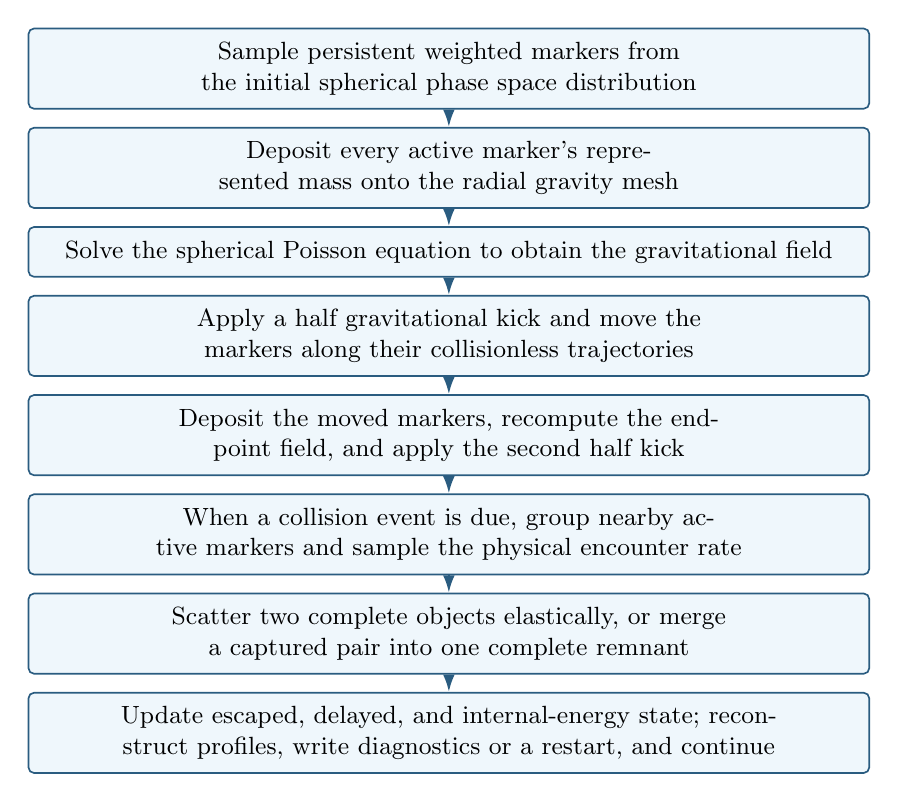
\begin{tikzpicture}[node distance=0.22cm]
\node[physicsflow] (wp1) {Sample persistent weighted markers from the initial spherical phase space distribution};
\node[physicsflow,below=of wp1] (wp2) {Deposit every active marker's represented mass onto the radial gravity mesh};
\node[physicsflow,below=of wp2] (wp3) {Solve the spherical Poisson equation to obtain the gravitational field};
\node[physicsflow,below=of wp3] (wp4) {Apply a half gravitational kick and move the markers along their collisionless trajectories};
\node[physicsflow,below=of wp4] (wp5) {Deposit the moved markers, recompute the endpoint field, and apply the second half kick};
\node[physicsflow,below=of wp5] (wp6) {When a collision event is due, group nearby active markers and sample the physical encounter rate};
\node[physicsflow,below=of wp6] (wp7) {Scatter two complete objects elastically, or merge a captured pair into one complete remnant};
\node[physicsflow,below=of wp7] (wp8) {Update escaped, delayed, and internal-energy state; reconstruct profiles, write diagnostics or a restart, and continue};
\draw[physicsarrow] (wp1) -- (wp2);
\draw[physicsarrow] (wp2) -- (wp3);
\draw[physicsarrow] (wp3) -- (wp4);
\draw[physicsarrow] (wp4) -- (wp5);
\draw[physicsarrow] (wp5) -- (wp6);
\draw[physicsarrow] (wp6) -- (wp7);
\draw[physicsarrow] (wp7) -- (wp8);
\end{tikzpicture}
\end{figure}

\subsubsection{Purpose and state variables}
\label{sec:wpic-continuum}

The weighted particle--mesh module represents Vlasov--Poisson and
Boltzmann--Poisson evolution with moving phase space markers.  Let
\(f(t,r,w,\eta)\) be the mass distribution function, \(r\) physical radius,
\(w\) radial peculiar velocity, and \(\eta=L^2/2\), where \(L\) is the
magnitude of specific angular momentum.  Integrating over the spatial angles
and the tangential velocity azimuth gives
\[
 \dd M=8\pi^2 f\,\dd r\,\dd w\,\dd\eta,
 \qquad \rho(t,r)=\frac{2\pi}{r^2}\int f\,\dd w\,\dd\eta .
                                                               \tag{PIC0a}
\]
Thus \(f\) has units of mass per spatial volume per velocity volume.  With
Hubble rate \(H(t)\), the Boltzmann--Poisson equations are
\[
 \partial_t f+(Hr+w)\partial_r f+
 \left(\frac{2\eta}{r^3}-\Phi_r-Hw\right)\partial_w f=C[f],
                                                               \tag{PIC0b}
\]
Here \(\rho_{\rm src}\) is the gravitational source density: total density
for an isolated static halo, or the prescribed background-subtracted source
for the expanding module. The enclosed source mass and force follow from
Poisson's equation.

\[
 \frac1{r^2}\partial_r(r^2\Phi_r)=4\pi G\rho_{\rm src},
 \qquad \Phi_r=\frac{\partial\Phi}{\partial r}.          \tag{PIC0c}
\]
Here \(G\) is Newton's constant and \(\Phi\) is the peculiar gravitational
potential.  Static isolated calculations set \(H=0\) and use the full halo
density as \(\rho_{\rm src}\).  In an expanding total-density calculation,
\(\rho_{\rm src}=\rho-\bar\rho\), where \(\bar\rho\) is the homogeneous
background density; an already background-subtracted input enters directly.
An imposed central mass and the unresolved interior mass enter through the
inner enclosed-mass boundary condition.  The expanding background and its
exact orbital update are derived in Section~\ref{sec:wpic-expanding-kdk}.

The Vlasov--Poisson equations follow by setting \(C[f]=0\).  In that limit
\(f\) remains constant along the characteristics of (PIC0b).  The particle
method follows those trajectories and deposits their positive masses to
solve (PIC0c).  Local collision sampling supplies \(C[f]\) when encounters
are enabled.  The subhalo operator also evolves each object's mass
and internal energy, so its state includes those additional properties.

The code samples each occupied part of the distribution with many markers.
In the source, \code{WeightedPICMarker} is the record that stores one marker's
complete persistent physical and bookkeeping state:
\[
 (m_p,r_p,w_p,\eta_p,E_{{\rm int},p},
   \sigma_{{\rm int},p},I_p,s_p),
 \qquad \eta_p=\frac{L_p^2}{2},
\]
where \(m_p\) is represented mass, \(r_p\) is areal radius, \(w_p\) is radial
velocity, \(L_p\) is angular momentum magnitude, and
\(\eta_p=L_p^2/2\) is the angular momentum coordinate used by the solver.
Furthermore, \(E_{{\rm int},p}\) is unresolved internal energy,
\(\sigma_{{\rm int},p}\) is its one-dimensional internal velocity dispersion,
\(I_p\) is a persistent integer identifier, and \(s_p\) records whether the
marker is active, delayed inside the unresolved central region, or escaped.
A collisionless orbit update changes \(r_p\) and \(w_p\) while
keeping \(m_p\), \(\eta_p\), \(E_{{\rm int},p}\), and
\(\sigma_{{\rm int},p}\) fixed.  Elastic collisions change \(w_p\) and
\(\eta_p\), but leave both complete marker masses unchanged.  In the Plummer
subhalo operator, capture replaces two whole objects by one remnant of mass
\(m_i+m_j\) and increases its \(E_{\rm int}\).  Both the material SIDM
operator and the Plummer encounter operator accept unequal positive marker
masses.  The field solve uses those same masses on the radial mesh, so the
calculation alternates between continuous marker orbits and mesh-based
gravity without reverting to an equal-mass approximation.

This chapter is restricted to the Newtonian Vlasov--Poisson and
Boltzmann--Poisson WPIC code.  The separate Einstein--Vlasov WPIC
implementation is documented in
Section~\ref{sec:weighted-einstein-vlasov-pic}; it is collisionless and is not
a substitute for the Newtonian collision paths described here.

This representation is useful when a phase space cell contains a sharp orbit
boundary.  Several markers can occupy different positions inside that cell
and follow their individual characteristics.  Orbit integration and field
deposition are implemented in \path{cpu/include/ev/weighted_vlasov_pic.hpp}.
Local elastic scattering is in
\path{cpu/include/ev/weighted_vlasov_pic_collisions.hpp}.  The conservative bridge
back to cell-average \(f(r,w,\eta)\) is in
\path{cpu/include/ev/weighted_vlasov_pic_phase_remap.hpp}.  The two-clock event
controller is in
\path{cpu/include/ev/weighted_vlasov_pic_event_scheduler.hpp}.  The complete
transport--collision--reconstruction event is assembled in
\path{cpu/include/ev/weighted_pic_boltzmann_event.hpp}.
Unequal-mass elastic scattering and inelastic capture for resolved Plummer
subhalo encounters are in
\path{cpu/include/ev/weighted_vlasov_pic_subhalo_collisions.hpp}.

\subsubsection{Step 1: turn cell mass into marker mass}

The spherical phase space measure is
\[
 \dd\Gamma=8\pi^2\,\dd r\,\dd w\,\dd\eta.
\]
Therefore a cell average \(f_{ijk}\) contains the physical mass
\[
 M_{ijk}=8\pi^2f_{ijk}\Delta r_i\Delta w_j\Delta\eta_k. \tag{PIC1}
\]
VENUS first constructs every \(M_{ijk}\) and its cumulative sum.  A set of
evenly spaced mass strata selects source cells from that cumulative sum.  This
gives approximately equal marker masses while retaining the exact total:
\[
 \sum_p m_p=\sum_{ijk}M_{ijk}.                            \tag{PIC2}
\]
The phase-grid initializer chooses a common marker mass from the nearest floating-point values
around the exact quotient.  The same selected mass is assigned to every
marker.  Equation (PIC2) is then satisfied to floating-point accuracy while
an initially quiet equal-mass sample is obtained.  Equality is an initializer
choice, not a collision restriction: restart or adaptive marker populations
may contain unequal positive masses.

Let \(N_{\rm occupied}\) be the number of source phase space cells with
positive represented mass, \(N_{\rm per\ cell}\) the requested nominal number
of markers for each such cell, and \(N_{\rm budget}\) the global upper limit on
the total marker count.  The nominal marker count is
\[
 N_p=\min(N_{\rm occupied}N_{\rm per\ cell},N_{\rm budget}). \tag{PIC3}
\]
The defaults are 32 markers per occupied cell and a global limit of one
million.  Selecting cells through mass strata lets a very small tail remain in
the represented total without assigning one compulsory marker to every tiny
tail cell.

The central source code is:
\codesource{WPIC marker initializer}
{\path{cpu/include/ev/weighted_vlasov_pic.hpp}}
{Converts positive phase space cell masses into a deterministic weighted-marker
 realization with the same represented total mass}
\begin{lstlisting}[language=C++]
cell_mass = 8.0 * PI * PI * f[q]
          * dr[i] * dw[j] * deta[k];

selected = systematic_sources(cells, marker_count,
                              total_mass, offset);
marker.mass = total_mass / marker_count;
\end{lstlisting}


\paragraph{Analytic radial halo initialization.}
The power-law halo task constructs its particles directly in
\code{initialize_markers} in \path{cpu/src/drivers/expanding_wpic.cpp}.
It assigns a specified number of quiet velocity pairs to each occupied
radial source cell. If cell $j$ contains mass $\Delta M_j$ and is sampled
by $N_j$ markers, each marker in that cell has mass
\begin{equation}
 m_p=\frac{\Delta M_j}{N_j}.
 \label{eq:analytic-radial-marker-mass}
\end{equation}
The uniform central source is sampled by the same rule. A common final
normalization factor makes the represented resolved mass equal to its
specified total. The radial cell masses differ, so a fixed marker count
per radial cell produces unequal masses across the halo. Optional angular importance strata divide
each source mass among the selected angular intervals before assigning
its quiet pairs. The literal assignment is
\codesource{Masses in the analytic radial halo sampler}
{\path{cpu/src/drivers/expanding_wpic.cpp}, \code{initialize_markers}, lines 1027--1032}
{Divides the source-shell mass in an angular stratum among its two markers per quiet pair}
\begin{lstlisting}[language=C++]
                const double marker_mass =
                    shell_mass * represented_mass_fraction
                    / static_cast<double>(2 * stratum_pairs);
\end{lstlisting}
Here \code{represented_mass_fraction} is the fraction of the source-shell
mass assigned to the stratum, and \code{stratum_pairs} is its number of
quiet pairs. The ordinary sampler has one angular stratum with fraction
one. In collisionless relaxation, these masses are quadrature weights
for the gravitational source. In the subhalo encounter model,
each is also the physical mass of one subhalo and enters its pair cross
section. Increasing the number of such markers at fixed source mass
therefore changes the physical subhalo population. Its mass distribution
must be specified along with the halo density and velocity distribution.

\subsubsection{Step 2: choose positions inside each source cell}

For a piecewise-constant cell, VENUS uses shifted low-discrepancy coordinates
in \(r,w,\eta\).  They spread the markers across the cell more evenly than
independent random draws.  The shift is generated from the marker identifier,
source-cell identifier, seed, and coordinate number.  Repeating a run with the
same seed therefore produces the same markers.

An analytic equilibrium supplies more information than a cell average.  In
that case the density-aware initializer proposes continuous points inside the
cell and accepts them with probability
\[
 P_{\rm accept}=\frac{f(r,w,\eta)}{f_{\rm bound}},        \tag{PIC4}
\]
where \(f_{\rm bound}\) is a verified upper bound for that cell.  A uniform
number \(z\) in \((0,1)\) is drawn from the counter-based sequence, and the
point is accepted when
\[
 z f_{\rm bound}\leq f(r,w,\eta).                        \tag{PIC5}
\]
Equations (PIC4)--(PIC5) sample the continuous distribution inside a cell.
They are especially important when the energy support cuts through an
\(\eta\) cell.

For a distribution symmetric in radial velocity, markers are emitted in
adjacent pairs with
\[
 (m,r,w,\eta),\qquad(m,r,-w,\eta).                       \tag{PIC6}
\]
Their initial radial momentum cancels exactly.  The code checks the cell
masses and velocity faces before enabling this quiet pairing.

\subsubsection{Step 3: deposit marker mass on the spherical mesh}

Gravity needs a radial density.  Define the volume coordinate
\[
 q=\frac{r^3}{3},\qquad
 \Delta V_i=4\pi(q_{i+1/2}-q_{i-1/2}).                  \tag{PIC7}
\]
Between neighboring shell centers \(q_i\leq q_p\leq q_{i+1}\), cloud-in-cell
deposition uses
\[
 a_{pi}=\frac{q_{i+1}-q_p}{q_{i+1}-q_i},\qquad
 a_{p,i+1}=1-a_{pi}.                                    \tag{PIC8}
\]
The two weights are nonnegative and add to one.  Near a physical boundary,
the in-domain weights are normalized again so that their sum remains one.

The expanding origin-parity path needs one additional construction.  Its
markers remain active while crossing the unresolved physical region
\(0\leq r_p<r_{\min}\), rather than reflecting at the innermost field face
\(r_{\min}\).  Define
\[
 q_f=\frac{r_{\min}^3}{3},\qquad
 \Delta q_0=2(q_0-q_f),\qquad
 W_q=\min(\Delta q_0,q_f),                               \tag{PIC8a}
\]
where \(q_f\) is the volume coordinate of the inner face, \(q_0\) is the
center of the first resolved shell, \(\Delta q_0\) is that shell's width in
\(q\), and \(W_q\) is the inner handoff width.  The minimum with \(q_f\)
keeps the handoff inside the physical range \(q\geq0\).  For a marker with
\(q_p=r_p^3/3<q_f\), VENUS forms
\[
 s_p=\operatorname{clip}\!\left[
       \frac{q_p-(q_f-W_q)}{W_q},0,1\right],
 \qquad f_p=s_p^2(3-2s_p),                               \tag{PIC8b}
\]
where \(\operatorname{clip}(x,0,1)\) limits \(x\) to the closed interval
\([0,1]\), \(s_p\) is the dimensionless position through the handoff, and
\(f_p\) is the fraction of marker \(p\)'s cloud assigned to the resolved
mesh.  The ordinary normalized CIC or TSC face stencil
\(a^{\rm face}_{pi}\), evaluated at \(r_{\min}\), is frozen below the face
and partitioned as
\[
 \widetilde a_{pi}=f_p a^{\rm face}_{pi},\qquad
 h_p=1-f_p,\qquad
 \sum_i\widetilde a_{pi}+h_p=1.                          \tag{PIC8c}
\]
Here \(\widetilde a_{pi}\) is the weight delivered to resolved shell \(i\)
and \(h_p\) is the complementary weight delivered to the unresolved inner
gravity carrier.  For \(q_p\geq q_f\), the ordinary position-dependent
stencil is used and \(h_p=0\); for \(q_p\leq q_f-W_q\), \(f_p=0\) and the
whole marker is carried inside.  Because \(f_p\) and its first derivative
match continuously at both ends, a marker crossing \(r_{\min}\) changes the
resolved and central source smoothly.

VENUS deposits extensive quantities first:
\[
 \begin{aligned}
 M_i&=\sum_p \widetilde a_{pi}m_p,&
 P_{r,i}&=\sum_p \widetilde a_{pi}m_pw_p,\\
 R_{2,i}&=\sum_p \widetilde a_{pi}m_pw_p^2,&
 T_{2,i}&=\sum_p \widetilde a_{pi}m_p\frac{2\eta_p}{r_p^2}.
 \end{aligned}                                           \tag{PIC9}
\]
Here \(i\) labels a resolved radial shell and the sum over \(p\) runs over
active markers.  Thus \(M_i\) is deposited represented mass,
\(P_{r,i}\) is deposited radial momentum, \(R_{2,i}\) is the mass-weighted
radial second moment (the deposited sum of \(w_p^2\)), and \(T_{2,i}\) is the
mass-weighted tangential second moment (the deposited sum of the squared
tangential speed \(2\eta_p/r_p^2\)).
In an ordinary reflecting calculation,
\(\widetilde a_{pi}=a_{pi}\).  In the origin-parity handoff it has the
meaning in equation (PIC8c).
It then divides by \(\Delta V_i\) to form physical shell averages.  Since
\(\sum_i\widetilde a_{pi}+h_p=1\), summing the deposited shell masses and
the unresolved carrier mass gives
\[
 \sum_i M_i+M_{\rm hid}
 =\sum_p m_p,\qquad M_{\rm hid}=\sum_p h_pm_p.           \tag{PIC10}
\]
Thus each marker contributes exactly \(f_pm_p\) to the boundary cloud and
\((1-f_p)m_p\) to the inner carrier: no represented mass is created or
lost.  The carrier is a mass-only unresolved source for gravity; for markers
that are wholly resolved, the usual partition-of-unity proof also applies to
every raw moment in equation (PIC9).  The Poisson solve includes
\(M_{\rm hid}\) as central enclosed mass. Equations (PIC8a)--(PIC8c)
transfer the represented mass continuously between the boundary cloud and
the unresolved central source as the marker crosses \(r_{\min}\).
The marker retains its physical mass and phase space coordinates.

The current Poisson routine represents shell mass as
\(4\pi r_i^2\rho_i\Delta r_i\).  The adapter therefore passes
\[
 \rho_i^{\rm field}=\frac{M_i}{4\pi r_i^2\Delta r_i}.   \tag{PIC11}
\]
Equation (PIC11) makes the mass seen by the Poisson solver exactly equal to
the shell mass \(M_i\); the same field solve adds \(M_{\rm hid}\) separately
as the unresolved central source, so its total represented source remains the
right-hand side of equation (PIC10).

Below the first physical mesh face, \(r_f=r_{\min}\), the Poisson solver
continues the unresolved source as a uniform sphere. Let \(M_f\) be the
enclosed source mass at that face, \(M_c\) a prescribed central point mass,
and \(\Phi_f=\Phi(r_f)\). For expanding \code{total_density} input,
\(M_f=M_c+M_{\rm hid}-4\pi\bar\rho r_f^3/3\), where
\(\bar\rho\) is the homogeneous background density. With
\code{density_contrast} input, the represented mass is already the
source contrast and \(M_f=M_c+M_{\rm hid}\). The continuation is
\[
 \Phi_r(r)=\frac{GM_c}{r^2}
          +\frac{G(M_f-M_c)}{r_f^3}r,\qquad 0<r<r_f,       \tag{PIC11a}
\]
\[
 \Phi(r)=\Phi_f+GM_c\left(\frac{1}{r_f}-\frac{1}{r}\right)
       +\frac{G(M_f-M_c)}{2r_f^3}(r^2-r_f^2).             \tag{PIC11b}
\]
Integrating the uniform density gives an enclosed mass proportional to
\(r^3\), which produces the linear force in (PIC11a). Integrating that
force from \(r_f\) gives (PIC11b). Both quantities join the resolved field
continuously at the face. An empty central cavity with \(M_f=M_c=0\)
therefore has zero force even when the first resolved shell contains matter.
The code samples the face mass and potential before applying this continuation:
\codesource{Gravitational field inside the first mesh face}
{\path{cpu/include/ev/vlasov_poisson.hpp}; \path{gpu/src/wpic_vlasov_poisson.cu}}
{Continue the enclosed source as a uniform central sphere, separating a prescribed point mass}
\begin{lstlisting}[language=C++]
const double r0 = face_resolved ? field.radial_edge.front() : r.front();
const double phi0 = face_resolved ? field.phi_edge.front() : field.phi.front();
const double face_force = face_resolved
    ? p.vp_gravity * field.source_mass_edge.front() / (r0 * r0)
    : field.phi_r.front();
\end{lstlisting}
The unresolved sphere supplies a force approximation inside \(r_f\).
Scientific profiles at nearby radii require comparison with a smaller
\(r_f\) and sufficient radial and particle resolution.

\subsubsection{Step 4: solve gravity and move the markers}

The deposited mass is sent through the ordinary spherical Poisson solver.
Write
\[
 g(t,r)=-\partial_r\Phi(t,r),
\]
where \(\Phi\) is the Newtonian gravitational potential and \(g\) is the
signed radial gravitational acceleration.  For positive enclosed mass,
\(g<0\), so gravity points inward.  Each active marker then follows
\[
 \dot r_p=w_p,\qquad
 \dot w_p=\frac{2\eta_p}{r_p^3}+g(t,r_p)
          =\frac{2\eta_p}{r_p^3}-\Phi_r(t,r_p).          \tag{PIC12}
\]
The library exposes both a generic frozen-field orbit adapter and a
self-consistent endpoint-field KDK update.  The generic adapter calls the same
VENUS characteristic machinery used by the grid solver, including ordinary
integration and selective Levi--Civita retry.  It is used by the frozen-field
event module.

The current static/expanding production runner uses a self-consistent KDK
step:
\begin{enumerate}
\item deposit markers at \(t^n\) and solve \(\Phi^n\);
\item apply one half gravitational kick and an exact central-force drift;
\item deposit the drifted markers at \(t^{n+1}\) and solve \(\Phi^{n+1}\);
\item apply the endpoint half kick.
\end{enumerate}
The drift formula and expanding variables are derived in
Section~\ref{sec:wpic-expanding-kdk}.

Marker states distinguish active, delayed-inner, and escaped mass.  A restart
stores every marker, its state, weight, \(\eta\), persistent identifier,
unresolved internal energy, delayed-boundary data, both random samplers, both
elapsed event-clock ages, time, and step. The self-consistent KDK path
reconstructs its radial field from the stored markers. The static Boltzmann
event path also stores the field held between potential updates.

\subsubsection{Step 5: form local collision shells}

Elastic SIDM scattering is local in position.  At the start of a collision
interval, VENUS sorts the active markers by radius and divides the sorted list
into shells.  The nominal shell contains 4096 markers, following the SphDSMC
construction used for the Frank benchmark.  The two shell faces are placed
halfway in the volume coordinate \(q=r^3/3\) between the last marker on one
side and the first marker on the other side.  This gives
\[
 V_s=\frac{4\pi}{3}\left(r_{s,+}^3-r_{s,-}^3\right),
 \qquad
 n_s=\frac{N_s}{V_s},\qquad
 n_{{\rm partner},s}=\frac{N_s-1}{V_s},\qquad
 \rho_s=\frac{\sum_{i\in s}m_i}{V_s}.                   \tag{PIC13}
\]
Here \(N_s\) is the number of complete markers in shell \(s\), \(m_i\) is the
represented mass of marker \(i\), \(n_s\) is the marker number density, and
\(\rho_s\) is mass density.  A chosen marker cannot collide with itself, so
its finite-shell density of available partners is
\(n_{{\rm partner},s}=(N_s-1)/V_s\).  The familiar continuum replacement
\(n_{{\rm partner},s}\simeq n_s\) has relative error \(1/N_s\).  Define the
shell's mass-weighted mean radial velocity and one-dimensional orbital
velocity dispersion by
\[
 M_s=\sum_{i\in s}m_i,\qquad
 \overline w_s=\frac{1}{M_s}\sum_{i\in s}m_iw_i,        \tag{PIC14a}
\]
\[
 \sigma_{v,s}^{\,2}=\frac{1}{3M_s}
 \sum_{i\in s}m_i\left[
   (w_i-\overline w_s)^2+\frac{2\eta_i}{r_i^2}
 \right].                                               \tag{PIC14b}
\]
The symbols \(r_i,w_i,\eta_i\) are marker radius, radial velocity, and half
the squared angular momentum.  Therefore \(2\eta_i/r_i^2\) is the squared
tangential speed.  The factor \(1/3\) converts the total three-dimensional
random kinetic variance into a one-dimensional dispersion.

For a sampled unordered pair \(i,j\), let
\(u_{ij}=|\bm v_i-\bm v_j|\) be relative speed and
\(\Sigma_{ij}(u_{ij})\) its physical pair area.  The tangential directions
are not stored in spherical phase space, so VENUS samples their relative
azimuth deterministically.  It then evaluates the collision-rate-weighted
mean free path directly from the evolving distribution:
\[
 \boxed{\displaystyle
 \lambda_s=
 \frac{\langle u_{ij}\rangle_s}
 {n_{{\rm partner},s}\left\langle
 u_{ij}\Sigma_{ij}(u_{ij})\right\rangle_s}}.             \tag{PIC14c}
\]
Angle brackets denote an average over unordered marker pairs and relative
tangential azimuth.  All pairs are used when the shell contains at most 512
unordered pairs; otherwise 512 deterministic pair samples are used.  For a material cross section per
mass \(s(u)=\sigma(u)/m\),
\[
 \Sigma_{ij}(u)=\frac{m_i+m_j}{2}s(u).
\]
For \(N_s\) equal masses and constant \(s\), equation (PIC14c) gives
\[
 \lambda_s=\frac{N_s}{N_s-1}\frac{1}{\rho_s s}.
\]
It approaches Frank and Tokayer's continuum result
\(\lambda_s=1/(\rho_s s)\) as \(N_s\) grows.  Retaining the finite-\(N_s\)
factor makes the locality diagnostic exactly consistent with the
unordered-pair trial law in equation (PIC17), including in a sparse shell.
For a velocity-dependent interaction, \(\sigma_{v,s}\) describes how broad
the evolving velocity distribution is, while equation (PIC14c) uses the full
sampled distribution rather than replacing it by one guessed RMS speed.  This
distinction matters when a low-speed tail has a much larger cross section.

If the shell width exceeds \(\lambda_s\), the shell is divided into two
equal-population children.  The criterion is applied recursively to each child.  Refinement
continues down to the configured minimum population.  The history output
records
\[
 \max_s \frac{r_{s,+}-r_{s,-}}{\lambda_s}.               \tag{PIC15}
\]
A value below one verifies that an accepted event joins markers within one
mean free path.  A production run can request a hard stop when equation
(PIC15) reaches one.

The source code implements this construction directly:
\codesource{WPIC adaptive collision-shell builder}
{\path{cpu/include/ev/weighted_vlasov_pic_collisions.hpp}}
{Measures the velocity-averaged mean free path and recursively divides a
 radial shell when its width is not local}
\begin{lstlisting}[language=C++]
const auto mfp = velocity_averaged_mean_free_path(
    markers, radius_order, begin, end, shell.volume,
    parameters, collision_options);
shell.mean_free_path = mfp.mean_free_path;
shell.orbital_velocity_dispersion =
    mfp.orbital_velocity_dispersion;

if (shell_width > shell.mean_free_path
    && shell_count >= 2 * minimum_shell_markers) {
    build_shell(left_half);
    build_shell(right_half);
}
\end{lstlisting}

\subsubsection{Step 6: choose the collision pairs}

Every pair of markers in one shell is physically eligible.  VENUS samples the
realized events with Bird's no-time-counter method.  Define
\[
 {\cal K}_{ij}(u)=u\Sigma_{ij}(u),
 \qquad {\cal K}_{\max}\geq
 \max_{a,b\in s}{\cal K}_{ab}(|\bm v_a-\bm v_b|).       \tag{PIC16}
\]
The symbol \({\cal K}_{ij}\) is the pair collision kernel: relative speed
times physical pair area.  It has dimensions of volume per time.
A Poisson process is a random event-counting model with independent waiting
intervals: for a constant rate \(\nu\), the chance of no event during
\(\Delta t\) is \(e^{-\nu\Delta t}\), and the waiting time to the next event
has an exponential distribution.  This statistical use of ``Poisson'' is
different from the Poisson field equation used for gravity.  The trial-event
clock is such a process with rate
\[
 \nu_{\rm trial}=\frac{N_s-1}{2}\,n_s{\cal K}_{\max}.    \tag{PIC17}
\]
If \(z_1\) is uniform on \((0,1)\), the time to the next trial is
\[
 \delta t_{\rm trial}=-\frac{\ln z_1}{\nu_{\rm trial}}. \tag{PIC18}
\]
For that trial, two distinct marker indices are drawn uniformly from the
shell.  With \(u=|\bm v_a-\bm v_b|\), a second uniform number \(z_2\) accepts
the pair when
\[
 z_2 < \frac{{\cal K}_{ab}(u)}{{\cal K}_{\max}}.         \tag{PIC19}
\]
Equations (PIC17)--(PIC19) make the accepted-pair rate proportional to
\(f(\bm v_a)f(\bm v_b)u\Sigma_{ab}(u)\).  The calculation visits the realized
trials and scales as \(N_p\log N_p+N_{\rm trial}\), including the radial sort.

The corresponding code is:
\codesource{WPIC no-time-counter collision sampler}
{\path{cpu/include/ev/weighted_vlasov_pic_collisions.hpp}}
{Draws trial times and distinct local marker pairs, then accepts each pair
 against the verified relative-speed--cross-section majorant}
\begin{lstlisting}[language=C++]
clock += -std::log(rng.uniform_open()) / trial_rate;
ia = rng.uniform_index(shell_count);
ib = distinct_uniform_index(shell_count, ia);

u_sigma = relative_speed * pair_total_cross_section(
    relative_speed, first_mass, second_mass, ...);
if (rng.uniform_open() * majorant_u_sigma < u_sigma) {
    scatter_pair(ia, ib);
}
\end{lstlisting}

Active markers may have unequal represented masses.  Each accepted elastic
event acts on the two complete masses in their mass-weighted centre-of-mass
frame.  Neither marker is split and both masses remain unchanged.

\subsubsection{Step 7: draw the outgoing direction}

A reduced spherical marker stores \(w=v_r\) and \(\eta=L^2/2\).  At its
current radius, its tangential speed is
\[
 v_t=\frac{\sqrt{2\eta}}{r}.                            \tag{PIC20}
\]
Spherical symmetry makes the tangential azimuth uniformly distributed.
VENUS draws an azimuth \(\alpha\) and lifts the marker to
\[
 \bm v=(w,v_t\cos\alpha,v_t\sin\alpha).                \tag{PIC21}
\]

At the exact coordinate origin, a finite spherical distribution has
\(\eta=0\). The stored \(|w|\) is the speed, and its Cartesian direction
is sampled isotropically. After scattering, the full outgoing speed is
stored with zero angular momentum, so the complete kinetic energy is
retained. The Cartesian pair update still conserves its vector momentum.
The mean projection along any reference axis is zero and its second moment
is \(w^2/3\). Shell dispersions, mean-free-path estimates, and collision
clocks use this same isotropic distribution. A positive radius whose square
underflows cannot represent a newly generated transverse energy in
\(\eta=r^2v_t^2/2\); the material operator rejects that state before any
collision is applied.
For an accepted pair, define
\[
 M_{12}=m_1+m_2,\qquad
 \bm V=\frac{m_1\bm v_1+m_2\bm v_2}{M_{12}},
 \qquad \bm u=\bm v_1-\bm v_2.                         \tag{PIC22}
\]
Here \(m_1,m_2\) are the complete marker masses, \(M_{12}\) is their sum,
\(\bm V\) is their centre-of-mass velocity, and \(u=|\bm u|\).

The differential cross section selects the direction of \(\bm u'\).  Write
\(\mu=\cos\theta\), where \(\theta\) is measured from \(\bm u\), and let
\(\psi\) be the azimuth around \(\bm u\).  For isotropic scattering, two
uniform numbers \(z_3,z_4\) give
\[
 \mu=2z_3-1,
 \qquad \psi=2\pi z_4.                                 \tag{PIC23}
\]

For the Yukawa--Born kernel, the numerical parameters \(m_\chi\) and
\(m_\phi\) set the speed scale \(m_\phi/m_\chi\), and
\(u=|\bm u|\) is the pair's relative speed defined in equation (PIC22).
Section~\ref{sec:yukawa-material-units} derives the amplitude and speed
conversion from physical particle masses and coupling to material-SIDM code
units.
With the abbreviations \(a=m_\phi^2\) and
\(b=m_\chi^2u^2/2\),
\[
 \frac{\dd\sigma}{\dd\Omega}\propto
 \frac{1}{[a+b(1-\mu)]^2},
 \quad a=m_\phi^2,
 \quad b=\frac{m_\chi^2u^2}{2}.                       \tag{PIC24}
\]
VENUS integrates this expression analytically.  A uniform \(z_3\) samples
the probability above the selected cosine.  With
\(y=(m_\chi u/m_\phi)^2\), the stable inverse is
\[
 \mu=1-\frac{2z_3}{1+y(1-z_3)}.                         \tag{PIC25}
\]
It approaches the uniform cosine \(1-2z_3\) as \(y\to0\).  At large
\(y\), the implementation divides numerator and denominator by \(y\),
keeping the arithmetic bounded.  The same inverse is used by material WPIC
and SphDSMC.
\codesource{Yukawa scattering angle}
{\path{cpu/include/ev/finite_angle_boltzmann.hpp}}
{Actual branches of \code{bp_fa_yukawa_born_mu_from_unit}; \code{z} is the
 sampled probability and \code{y} is the squared relative speed ratio}
\begin{lstlisting}[language=C++]
if (y <= 1.0) {
    one_minus_mu = 2.0 * z / (1.0 + y * (1.0 - z));
} else {
    const double inverse_y = 1.0 / y;
    one_minus_mu = 2.0 * z * inverse_y / (inverse_y + (1.0 - z));
}
\end{lstlisting}
Equation (PIC25) draws more small-angle events when the differential cross
section is forward peaked.  The azimuth remains \(\psi=2\pi z_4\).

An orthonormal basis \((\widehat{\bm u},\bm e_1,\bm e_2)\) then gives
\[
 \widehat{\bm u}'=
 \mu\widehat{\bm u}
 +\sqrt{1-\mu^2}\left(\cos\psi\,\bm e_1
 +\sin\psi\,\bm e_2\right).                           \tag{PIC26}
\]
The outgoing velocities are
\[
 \bm v_1'=\bm V+\frac{m_2}{M_{12}}u\widehat{\bm u}',
 \qquad
 \bm v_2'=\bm V-\frac{m_1}{M_{12}}u\widehat{\bm u}'.  \tag{PIC27}
\]
Thus each accepted event preserves all three components of pair momentum and
the pair kinetic energy.  The reduced marker variables are updated with
\[
 w_p'=v_{p,r}',
 \qquad
 \eta_p'=\frac{r_p^2}{2}\left[(v_{p,y}')^2+(v_{p,z}')^2\right]. \tag{PIC28}
\]
Equation (PIC28) is the angular momentum redistribution.  Each collision can
move both markers to new values of \(L=\sqrt{2\eta}\).

The main source lines are:
\codesource{WPIC finite-angle elastic scatter}
{\path{cpu/include/ev/weighted_vlasov_pic_collisions.hpp}}
{Samples the outgoing relative direction, applies the unequal-mass
 centre-of-mass map, and returns the updated spherical marker variables}
\begin{lstlisting}[language=C++]
const double total_mass = first_mass + second_mass;
const BPFAVec3 centre = bp_fa_scale(
    bp_fa_add(
        bp_fa_scale(v1, first_mass),
        bp_fa_scale(v2, second_mass)),
    1.0 / total_mass);
const double mu = sample_scatter_mu(u, p, options, rng);
const double psi = 2.0 * PI * rng.uniform_open();
const BPFAVec3 relative_after =
    bp_fa_scale(
        scattered_relative_direction(relative, mu, psi), u);

out1 = bp_fa_add(
    centre,
    bp_fa_scale(relative_after, second_mass / total_mass));
out2 = bp_fa_sub(
    centre,
    bp_fa_scale(relative_after, first_mass / total_mass));
marker.eta = 0.5 * r * r * (out.y * out.y + out.z * out.z);
\end{lstlisting}

\subsubsection{Step 8: schedule orbital motion, field refreshes, and collisions}

The frozen-field event library keeps separate gravitational field and
collision clocks.  The first clock measures the elapsed time since the field
was refreshed.  In \path{weighted_pic_boltzmann_potential_timescale}, its
deadline uses the represented-mass-weighted root-mean-square field and rate:
\[
 T_\Phi=\eta_\Phi\min\left[
 \left(\frac{\sum_i\omega_i\Phi_i^2}
             {\sum_i\omega_i\dot\Phi_i^2}\right)^{1/2},
 \left(\frac{\sum_i\omega_i g_i^2}
             {\sum_i\omega_i\dot g_i^2}\right)^{1/2}
 \right].                                             \tag{PIC29}
\]
Here \(M_i\geq0\) is deposited shell mass,
\(\omega_i=M_i/\sum_jM_j\), \(g=-\Phi_r\) is the radial acceleration defined
in (PIC12), and a dot denotes the physical-time derivative calculated from
the current moments by \code{vp_potential_time_derivative}.  The source is
\path{cpu/include/ev/weighted_pic_boltzmann_event.hpp}, lines 145--203.
Each channel contributes only when both of its mean squares exceed
\((4096\epsilon_{\rm mach})^2\); otherwise its time is infinite, where
\(\epsilon_{\rm mach}\) is double-precision machine roundoff.  Zero represented
mass and the helper's expanding-background branch also return infinity.
The standalone static/expanding KDK drivers instead use the successive-field
maximum-norm clock in (PIC39a)--(PIC39c).
The second clock measures the elapsed time since the last collision update.
Its deadline is
 \[
 T_{\rm coll}=\eta_{\rm coll}\min_r
 \left[n_{\rm partner}(r)\left\langle
 u\Sigma_{ij}(u)\right\rangle_r\right]^{-1}.          \tag{PIC30}
\]
Here \(\eta_\Phi\) and \(\eta_{\rm coll}\) are accuracy parameters no larger
than one, and \(n_{\rm partner}(r)=(N_s-1)/V_s\) is the finite-shell partner
density at the shell containing \(r\).  The averages in equation (PIC30) are
measured from the current markers in the local collision shells.  The default
pilot uses 128 uniformly chosen pairs per shell.  For each pair it draws the
unresolved tangential azimuths and evaluates \(u\Sigma_{ij}(u)\) with the
actual two masses.  If the sample mean is \(\overline{\cal K}_s\)
and its standard error is \(e_s\), the scheduling rate uses
\[
 {\cal K}_{s,\rm schedule}=
 \min({\cal K}_{s,\max},\overline{\cal K}_s+4e_s).      \tag{PIC30a}
\]
The four-error buffer makes an accidentally long collision interval unlikely.
The exact majorant \({\cal K}_{s,\max}\) from equation (PIC16) still controls every
internal NTC substep.  Thus the outer clock follows the physical mean rate,
while the event generator retains its strict upper bound.

Let \(A_\Phi\) and \(A_{\rm coll}\) be the two elapsed clock ages.  The next
frozen-field orbit interval is
\[
 \Delta t=\min\left(T_\Phi-A_\Phi,
                    T_{\rm coll}-A_{\rm coll},
                    \Delta t_{\rm orbit,max}\right).  \tag{PIC31}
\]
The orbit integrator may take many internal steps during \(\Delta t\).  These
internal steps only move the markers.  The endpoint distribution is
reconstructed after a scheduled event.  This arrangement permits accurate
pericentre integration, including Levi--Civita retries, while keeping the
number of phase space remaps small.

The finite cap \(\Delta t_{\rm orbit,max}\) is also a clock-probe interval.
If the cap arrives before either physical deadline, VENUS deposits only the
radial mass and velocity moments needed to remeasure \(T_\Phi\) and
\(T_{\rm coll}\).  It keeps the current gravitational field and does not
construct the full phase space array at this probe.  If a newly measured
deadline is already shorter than its accumulated age, the corresponding
event is carried out immediately.  This catches a rapid departure from an
initial equilibrium without introducing an extra remap at every orbit step.

At the end of the interval, VENUS carries out the event whose deadline has
arrived:
\begin{enumerate}
\item If the collision deadline arrives first, move the markers through the
frozen potential, apply the local NTC collisions from Steps 5--7, and then
reconstruct the endpoint distribution.
\item If the potential deadline arrives first, move the markers, reconstruct
the endpoint distribution, deposit its mass, and solve for the new potential.
The collision age is retained, so the pending collision deadline continues
to approach.
\item If both deadlines arrive together and \(T_{\rm coll}<T_\Phi\), use the
collision-first order in item 1.
\item If both deadlines arrive together and \(T_\Phi\leq T_{\rm coll}\),
reconstruct and refresh the field first, and then apply the collision update.
\end{enumerate}

Only the clock associated with a completed event is reset.  For example, a
field refresh leaves \(A_{\rm coll}\) unchanged.  Several field refreshes can
therefore occur during one collision interval, and several collision updates
can occur during one field-refresh interval.  After each reconstruction,
VENUS measures the current timescales again and plans the next event with the
remaining clock ages.

The integrated state keeps both continuous markers and a reconstructed
phase space snapshot.  The snapshot contains a cell-average grid and, when
needed, a short list of continuous carrier markers described in Step 9.  A
Boolean flag records whether this combined snapshot describes the current
markers.  A collision-first event ends with reconstruction, so the flag is
true.  At a coincident potential-first event, VENUS reconstructs the snapshot,
solves for the field, and then scatters the markers.  The local collision does
not change any marker radius or the radial mass profile, so the new field is
still valid.  The velocity space snapshot is marked stale and is rebuilt only
when phase space output or the next grid synchronization requires it.  This
uses one velocity reconstruction at that endpoint.

The source expresses this rule directly:
\codesource{WPIC two-clock event scheduler}
{\path{cpu/include/ev/weighted_vlasov_pic_event_scheduler.hpp}}
{Chooses the next orbit interval and orders coincident field-refresh and
 collision events without resetting the other physical clock}
\begin{lstlisting}[language=C++]
WeightedPICEventPlan event = plan_weighted_pic_event(
    clock, t_phi, t_collision,
    eta_phi, eta_collision, orbit_cap);

execute_weighted_pic_event(
    event,
    [&] { advance_markers_in_frozen_field(event.orbit_interval); },
    [&] { reconstruct_endpoint_distribution(); },
    [&] { apply_local_ntc_collisions(collision_age); });
commit_weighted_pic_event(clock, event);
\end{lstlisting}

The production wrapper calls the same operations through one function:
\codesource{WPIC Boltzmann event wrapper}
{\path{cpu/include/ev/weighted_pic_boltzmann_event.hpp}}
{Assembles transport, deposition, collision sampling, phase space
 reconstruction, and event diagnostics into one accepted update}
\begin{lstlisting}[language=C++]
WeightedPICBoltzmannEventDiagnostics diagnostic =
    advance_weighted_pic_boltzmann_event(
        state, field_grid, phase_geometry, parameters,
        orbit_plan, event_options, collision_options,
        remaining_run_time);
\end{lstlisting}
The returned diagnostic states the selected ordering, the number of NTC
trials and accepted pairs, whether reconstruction occurred before or after
collision, and the marker mass before and after the event.

The collision sampler state and both clock ages belong in a restart.  This
preserves the physical time remaining to each event after a continuation.

\subsubsection{\texorpdfstring{Step 9: reconstruct cell-average \(f(r,w,\eta)\)}
{Step 9: reconstruct cell-average f(r,w,eta)}}

The marker ensemble is itself a sampled distribution function.  Gravity needs
the radial deposition in equations (PIC7)--(PIC11).  A phase space snapshot is
reconstructed at a scheduled endpoint, an output, or a restart conversion.
The event order in Step 8 determines whether that endpoint reconstruction is
performed before or after the NTC collision update.

VENUS first places each active marker in one radial cell, then groups markers
with exactly the same stored mass.  ``Exactly'' here means literal equality
of the stored floating-point mass, not membership in a tolerance bin; the
remap never combines two unequal packet masses into one projection pair.
Within each numerical projection group it sorts by kinetic energy evaluated
at the cell center.  The lowest and highest remaining energies form a pair;
marker IDs break exact ties.  Pairing across the occupied energy range gives
the nonnegative projection a broad moment interval while each member still
uses velocity cells near its own continuous velocity.  This grouping is only
a reconstruction device: the physical NTC collision sampler remains free to
pair different masses.  For group mass \(m_g\), one continuous marker pair
has target radial momentum and kinetic energy
\[
 P_*=m_g(w_1+w_2),
 \qquad
 K_*=m_g\left[\frac{w_1^2+w_2^2}{2}
 +\frac{\eta_1+\eta_2}{r_i^2}\right].                 \tag{PIC32}
\]
The remap finds nonnegative weights \(a_\ell\) on nearby pairs of velocity
cells such that
\[
 \sum_\ell a_\ell=1,
 \quad
 \sum_\ell a_\ell(w_{\ell1}+w_{\ell2})=P_*/m_g,
 \quad
 \sum_\ell a_\ell(E_{\ell1}+E_{\ell2})=K_*/m_g.       \tag{PIC33}
\]
It deposits \(m_ga_\ell\) into each member of pair \(\ell\).  An odd marker,
including a marker whose mass is unique in that radial cell, is paired with
an identical copy and each copy receives half the ordinary pair weight.  This
does not split or add a persistent marker; it is only a two-point
representation used while depositing one unchanged mass \(m_i\).  Thus a
discrete unequal-weight hierarchy can form ordinary equal-mass projection
groups, whereas a realistic continuously varying mass spectrum may leave
almost every group as a singleton.  The latter case is algebraically valid
but can be expensive and noisy; record the duplicated-singleton fraction,
projection cost, and carrier fraction, and refine both the velocity grid and
marker population before interpreting it.  The reconstructed
cell average is
\[
 f_{ijk}=\frac{M_{ijk}}{
 8\pi^2\Delta r_i\Delta w_j\Delta\eta_k}.             \tag{PIC34}
\]
Equations (PIC33)--(PIC34) preserve active marker mass, radial momentum, and
kinetic energy while keeping every cell mass nonnegative.  Hidden-inner and
escaped marker masses remain separate ledger entries.  A marker pair outside
the velocity domain stops the remap and reports whether the \(w\) or \(L\)
extent must be enlarged.

A continuous velocity can also lie inside the grid faces while its exact
moments lie outside the set formed by the nearby cell centers.  For example,
consider a marker with \(w=0\) and \(\eta=0\) on a cell-average grid whose
first \(\eta\) center is positive.  The marker belongs to the grid domain, but
every nonnegative combination of cell-center packets has positive kinetic
energy.  Placing the marker in the first cell would therefore add kinetic
energy.

VENUS searches a bounded neighborhood of velocity cells for the nonnegative
weights in equation (PIC33).  The option
\code{maximum_candidate_radius} limits this neighborhood, so the cost of one
difficult pair stays local.  If an in-domain pair still has no solution, the
pair can remain in continuous form as a reconstruction carrier.  Its marker
indices are stored in \code{carrier_marker_indices}.  The reconstructed state
then obeys
\[
 M_{\rm active}=\sum_{ijk}M_{ijk}+M_{\rm carrier},       \tag{PIC34a}
\]
and the two other budgets obey
\[
 \begin{aligned}
 P_{r,\rm active}&=P_{r,\rm grid}+P_{r,\rm carrier},\\
 K_{\rm active}&=K_{\rm grid}+K_{\rm carrier}.
 \end{aligned}                                          \tag{PIC34b}
\]
The carrier markers remain in the main marker ensemble.  Orbit motion,
radial gravity deposition, and NTC pair selection continue to include them.
The carrier list records the small part of the endpoint distribution that the
current velocity-cell centers cannot represent with exact moments.

The option \code{maximum_carrier_mass_fraction} is a hard cumulative upper
bound on \(M_{\rm carrier}/M_{\rm active}\).  Before retaining any unresolved
pair, VENUS adds that pair's full represented mass to the carrier mass already
accepted in the same remap and checks the resulting fraction.  The remap stops
rather than silently crossing the cap.  Its default value is zero, so the
first unresolved projection is reported immediately.  A diagnostic run may
set a small positive bound and measure how this fraction changes as marker
count and velocity resolution increase.  A production convergence sequence
requires the fraction to decrease under refinement.  A velocity outside the
grid faces always stops the remap, regardless of the carrier bound.

The bridge is called with:
\codesource{WPIC conservative phase space remap}
{\path{cpu/include/ev/weighted_vlasov_pic_phase_remap.hpp}}
{Projects continuous weighted markers onto cell averages while reporting any
 unresolved carrier mass and moment-closure residuals}
\begin{lstlisting}[language=C++]
WeightedPICPhaseRemapOptions remap_options;
remap_options.maximum_candidate_radius = 8;
remap_options.maximum_carrier_mass_fraction = 0.01;

WeightedPICPhaseRemapResult remap =
    remap_weighted_vlasov_pic_to_phase_space(
        markers, geometry, parameters, remap_options);

double represented_mass = std::accumulate(
    remap.cell_mass.begin(), remap.cell_mass.end(), 0.0);
represented_mass += remap.diagnostics.carrier_mass;
\end{lstlisting}

The useful remap cadence follows the event intervals in equations
(PIC29)--(PIC31), which are usually longer than an orbit-integrator substep.
Characteristic motion accumulates continuously on the markers, and equation
(PIC34) is evaluated once at a scheduled endpoint.  Convergence studies vary
the marker count, both clock tolerances, \(r_{\min}\), and all three grid
resolutions.
An out-of-domain velocity is a hard domain error rather than an implicit
boundary remap.  Equations (PIC34a)--(PIC34b) provide the mass, momentum, and
kinetic-energy closure conditions for every reconstruction.

\subsubsection{Initial conditions, provenance, and task interfaces}

There are two fresh-data routes in this module, and they produce different
objects.

\noindent\textbf{Expanding Vlasov--Poisson and subhalo route.}
The consuming task is \code{venus_cpu_subhalo_wpic}.  Its fail-closed frontend
is \path{cpu/src/apps/subhalo/expanding_wpic.cpp}.  In the shared driver,
\code{PowerLawInitialCondition} is the source class that evaluates the
normalized, tapered power-law density selected by the cusp exponent
\(\gamma\), and precomputes the shell and enclosed masses from which markers
are sampled.  This class and the \code{initialize_markers} sampler in
\path{cpu/src/drivers/expanding_wpic.cpp} create an in-memory
\code{std::vector<WeightedPICMarker>}, meaning a resizable list of the marker
records defined at the start of this chapter.  The first accepted state is
persisted as \path{restart_state.bin} in the requested output directory.
Before using it, verify the supported cusp exponent and cosmological
convention, positive marker weights, represented mass, marker--mesh support,
the reported initial density error, and an otherwise identical zero-collision
control.  Then refine the marker loading and radial mesh.

\noindent\textbf{Static material-SIDM route.}
The consuming task is \code{venus_cpu_sidm_wpic_constant}, selected by
\path{cpu/src/apps/sidm/wpic_constant.cpp} and implemented by
\path{cpu/src/drivers/sidm_wpic.cpp}.  A compatible Frank marker population can
be generated by
\path{cpu/tools/generate_frank_core_spherical_dsmc_restart.py}; its output is a
versioned \code{VENUSSPHDSMC1} persistent-marker restart.  The importer
\code{import_weighted_pic_frank_restart} in
\path{cpu/include/ev/weighted_pic_frank_restart_import.hpp} converts
\((r,v_r,L,m,I)\) to WPIC markers \((r,w,\eta,m,I)\), after which the runner
writes its own \path{restart_state.bin}.  Validate the restart magic and
version, unique identifiers, positive individual masses, represented mass,
radial support, initial equilibrium drift, shell locality, and collision rate.
An unequal-mass input must be imported in full; a marker-limited import is only
an equal-mass diagnostic and is not a convergence datum.

\noindent\textbf{Runnable expanding WPIC example.}
The WPIC task executables use command-line controls rather than the generic
\path{params.ini}.  This self-contained example enables both elastic subhalo
scattering and inelastic capture:
\codesource{\code{venus_cpu_subhalo_wpic}}
{\path{cpu/src/apps/subhalo/expanding_wpic.cpp};
 \path{cpu/src/drivers/expanding_wpic.cpp}}
{Selects the expanding subhalo task and owns its command-line setup,
 marker initialization, evolution, and output}
\begin{lstlisting}[basicstyle=\ttfamily\scriptsize]
cd VENUS/cpu
make venus_cpu_subhalo_wpic
make venus_cpu_vlasov_poisson_wpic_expanding

./venus_cpu_subhalo_wpic \
  --gamma 0.5 \
  --end-time 0.2 \
  --maximum-timestep 0.01 \
  --particles-per-radial-cell 512 \
  --subhalo-collision-strength 0.1 \
  --subhalo-velocity-scale 0.1 \
  --subhalo-plummer-area-per-mass 1 \
  --subhalo-low-speed-regularization 0.05 \
  --subhalo-collision-interval 0.01 \
  --subhalo-collision-timescale-fraction 0.1 \
  --subhalo-collision-cfl 0.2 \
  --subhalo-collision-maximum-substeps 256 \
  --threads 8 \
  --output-directory output/wpic_subhalo_example
\end{lstlisting}
For every strength, cusp, mesh, and marker loading, inspect the evolving
locality diagnostic before interpreting the profiles.  Set
\code{--subhalo-collision-strength 0} only in the compatibility driver for an
otherwise identical collisionless Vlasov--Poisson control; the task-specific
\code{venus_cpu_subhalo_wpic} frontend requires positive collision strength.
The static elastic SIDM runner can start from a generated equal-mass Frank
marker sample, while its importer and collision core also preserve unequal
masses stored by version-4/5 SphDSMC restarts; the runnable import is in
Section~\ref{sec:wpic-material-sidm-run}.  The value 256 in this short example
is only the administrative internal-loop guard.  High-rate unequal-mass
production uses 16384; the collision CFL still selects every physical NTC
substep.

\subsubsection{Running the integrated material-SIDM core case}
\label{sec:wpic-material-sidm-run}

The task-specific executable is
\code{venus_cpu_sidm_wpic_constant}.  It keeps the
markers, field, two clocks, collision sampler, and reconstructed snapshot in
one integrated event state.  Every step calls the high-level event advance
function shown in Step 8, so transport, collision sampling, reconstruction,
and conservation accounting share one event order.

The following commands generate a compatible equal-mass Frank marker object,
import all of its markers, and advance a short constant-cross-section
interval.  A gridded \code{EVLOGRST1} file is not accepted by
\code{--frank-restart}; that option requires the persistent-marker
\code{VENUSSPHDSMC1} format.
\codesource{\path{generate_frank_core_spherical_dsmc_restart.py} and
 \code{venus_cpu_sidm_wpic_constant}}
{\path{cpu/tools/generate_frank_core_spherical_dsmc_restart.py};
 \path{cpu/src/apps/sidm/wpic_constant.cpp};
 \path{cpu/src/drivers/sidm_wpic.cpp}}
{Generates the versioned Frank marker population, imports it into the
 constant-cross-section material-SIDM WPIC task, and advances the coupled
 field--collision state}
\begin{lstlisting}
python tools/generate_frank_core_spherical_dsmc_restart.py \
  --output output/frank_sphdsmc_50000.restart.bin \
  --particles 50000 --seed 5489 --radial-sampling stratified

make venus_cpu_sidm_wpic_constant
./venus_cpu_sidm_wpic_constant \
  --frank-restart output/frank_sphdsmc_50000.restart.bin \
  --output-directory output/sidm_wpic_constant \
  --end-time 0.0033 \
  --maximum-timestep 0.001 \
  --potential-event-eta 1.0 \
  --collision-event-eta 0.01 \
  --radial-cells 64 \
  --radial-velocity-cells 32 \
  --eta-cells 96 \
  --eta-grid-power 8 \
  --radial-velocity-maximum 5 \
  --angular momentum-maximum 400 \
  --sidm-cross-section constant \
  --sidm-sigma0 20.106192982974676 \
  --collision-strength 1 \
  --collision-cfl 0.2 \
  --collision-maximum-substeps 65536 \
  --collision-adaptive-shell-timestep \
  --collision-adaptive-maximum-interval 0.02 \
  --remap-candidate-radius 8 \
  --maximum-carrier-mass-fraction 0.01 \
  --threads 32
\end{lstlisting}
The optional \code{--marker-limit} performs a deterministic radial subsample
of the supplied equal-mass realization, then rescales it to
the full input mass.  This option is intended only for inexpensive inspection;
omitting it imports every marker with its
stored mass unchanged.  A limited import of an unequal-mass restart is
rejected because number-ranked subsampling could bias its phase space mass
profile; import all such markers.  The limited run's core-density diagnostic
is not quantitatively comparable with the full import or with a different
marker limit.  The core is defined by the innermost
\(\max[250,\operatorname{round}(2.5\times10^{-4}N_{\rm selected})]\)
selected markers.  Changing \(N_{\rm selected}\), while rescaling each
selected marker to represent the full mass, changes the enclosed mass and
radius that define ``core.''  Consequently \code{core_density},
\code{core_sigma_r2}, and \code{core_radius} from a marker-limited history
cannot be used as a physical convergence comparison.

The radial profiles use the conservative deposition in equations
(PIC7)--(PIC11) directly.  Every scheduled phase space reconstruction is
recorded in
\path{operator_mass_budget.csv}.  Its columns include the event order, marker
mass before and after, gridded mass, carrier mass, radial-momentum error,
kinetic-energy error, and maximum pair-projection error.  A final output
synchronization has event order \(-1\).

The restart stores the continuous markers, collision random-number state,
both event-clock ages, the frozen Poisson field, and the two current timescale
estimates. A continuation starts with \code{--pic-restart}. Restoring the
saved field preserves the potential interval already in progress. The next
collision or potential event then occurs at the same time as in uninterrupted
evolution.
\codesource{Static SIDM event continuation}
{\path{cpu/src/drivers/sidm_wpic.cpp};
 \path{cpu/include/ev/weighted_pic_boltzmann_event.hpp}}
{Retain the frozen field and the current physical event deadlines}
\begin{lstlisting}[language=C++]
state.field = checkpoint.frozen_field;
state.potential_timescale = checkpoint.potential_timescale_estimate;
state.collision_timescale = checkpoint.collision_timescale_estimate;
\end{lstlisting}
The saved control record authenticates the mesh, force and collision laws,
orbit tolerances, event controls, and thread count. End time and output
cadence may change on continuation. For a deliberate mesh or numerical-control change,
\code{--refresh-restart-field} recomputes the field and its timescales and
starts a new potential interval. It retains the collision age accumulated
since the last collision, so the physical gravity and collision laws retain
their saved values. The driver records this choice in
\path{restart_import.txt}. Legacy versions 1--6 contain particle initial data;
their import reconstructs the field and timescales and reports that operation.

Continuing in an existing output directory checks every saved history and
profile time against the selected checkpoint before opening output files.
If a saved diagnostic is later than that checkpoint, use a separate output
directory for the continuation. This preserves the original trajectory and
keeps each recorded history in time order. The expanding WPIC driver applies
the same check to its energy, virial, and collision histories.

\paragraph{Particle export and numerical-sample refinement.}
The inspection tool has an explicit conversion command,
\par\noindent\begin{minipage}{\linewidth}
\codesource{Export particle initial data}
{\path{cpu/tools/inspect_weighted_pic_restart.cpp}}
{Preserve the particle state and initialize a fresh field schedule}
\begin{lstlisting}[language=bash]
inspect_weighted_pic_restart INPUT --export-particles OUTPUT
\end{lstlisting}
\end{minipage}\par
It preserves particle masses, coordinates, internal state, identifiers,
random counters, time, and step. Its version-6 output initializes a new field
and event schedule at that physical time, with zero event ages and fresh
timescale estimates. This supplies particle initial data for a receiving
CPU or GPU task. Export requires a completed collision interval,
\code{collision_event_age=0}, and a distinct output file.

The refinement command divides each numerical marker into equal-mass
samples at the same phase space point:
\codesource{Refine the numerical particle sampling}
{\path{cpu/tools/refine_weighted_pic_restart.cpp}}
{Split numerical weights while preserving the represented distribution}
\begin{lstlisting}[language=bash]
refine_weighted_pic_restart INPUT OUTPUT FACTOR --reinitialize-field
\end{lstlisting}
The factor is an integer from 2 through 16. Refinement preserves the
mass-weighted spatial and velocity moments and assigns distinct identifiers
to the additional samples. It requires zero internal energy, zero internal
velocity dispersion, and a completed collision interval. These conditions
support collisionless or material-SIDM sampling studies. A subhalo
marker represents a physical object whose mass enters its encounter law;
such an object's mass distribution must be specified physically. A
frozen-field input requires the explicit \code{--reinitialize-field} option.
The output is version-6 particle initialization with the frozen field and
timescale estimates cleared and the potential-event age reset.

\paragraph{CPU material-SIDM local shell clocks.}
Let
\[
 \nu_s=n_{{\rm partner},s}
       \max_{i,j\in s}[u\Sigma_{ij}(u)]
\]
be the conservative NTC exposure rate in collision shell (s).  Reference
mode uses the fastest shell for every shell,
\[
 \delta t_{\rm fixed}=\min\left(
 \Delta t_{\rm op}-t,
 \frac{C_{\rm coll}}{\max_s\nu_s}\right).             \tag{PIC34c}
\]
With \code{--collision-adaptive-shell-timestep}, every shell has an
independent elapsed time \(t_s\) and instead takes
\[
 \delta t_s=\min\left(
 \Delta t_{\rm op}-t_s,
 \frac{C_{\rm coll}}{\nu_s}\right).                    \tag{PIC34d}
\]
The shells are disjoint and marker radii do not move inside the split
collision operator.  Threads therefore advance different shells concurrently
without changing their event rates.  After each local elastic update VENUS
refreshes the shell velocity moments and safe \(u\Sigma\) majorant; shell
faces, volume, density, and radial membership are reused.  The implementation
is structurally
\codesource{WPIC adaptive local shell clocks}
{\path{cpu/include/ev/weighted_vlasov_pic_collisions.hpp};
 \path{cpu/src/drivers/sidm_wpic.cpp}}
{Advances disjoint constant-cross-section shells with their own conservative
 collision exposure while retaining one synchronized outer event}
\begin{lstlisting}[language=C++]
for (shell : collision_shells) {
  while (shell.elapsed < operator_interval) {
    rate = shell.partner_density * shell.majorant_u_sigma;
    dt_shell = min(operator_interval - shell.elapsed,
                   collision_cfl / rate);
    apply_shell_ntc(shell, dt_shell, shell.local_substep);
    refresh_shell_velocity_majorant(shell);
  }
}
\end{lstlisting}
\code{--collision-adaptive-maximum-interval} caps the synchronized outer
collision batch; it is not a second local CFL.  In this CPU release the
reusable-shell path is deliberately restricted to constant cross section,
equal marker masses within each shell, and \(0<C_{\rm coll}\le1\).  The
velocity-dependent and unequal-mass material paths retain equation (PIC34c).
The reported \code{substeps} is the largest local count and
\code{shell_visits} is the sum over shells.  Omitting the flag retains the
mesh-wide reference schedule.

\subsubsection{Static and expanding self-consistent KDK}
\label{sec:wpic-expanding-kdk}

The expanding runner stores physical radius \(r=a(t)x\) and physical peculiar
radial velocity \(u\), where \(a(t)\) is the cosmological scale factor and
\(x\) is comoving radius.  The canonical radial momentum is
\[
 p=a u.
\]
For a power-law background
\[
 a(t)=a_0\left(\frac{\tau}{\tau_0}\right)^\alpha,
 \qquad \tau=t+t_{\rm off},
\]
\(\alpha\) is the expansion exponent and \(t_{\rm off}\) is the configured
time offset.  During a force-free drift the useful interval is
\[
 s(t_0,t_1)=\int_{t_0}^{t_1}\frac{\dd t}{a(t)^2}.
\]
Let \(\tau_0=t_0+t_{\rm off}\), \(\tau_1=t_1+t_{\rm off}\), and
\(\beta=1-2\alpha\).  The exact integral is
\[
 s=\frac{\tau_0}{a(t_0)^2}
 \begin{cases}
  \displaystyle
  \frac{\exp\!\left[\beta\ln(\tau_1/\tau_0)\right]-1}{\beta},
  &\beta\ne0,\\[8pt]
  \ln(\tau_1/\tau_0),&\beta=0.
 \end{cases}
\]
The code evaluates the numerator with \code{expm1} to avoid cancellation when
\(|\beta\ln(\tau_1/\tau_0)|\ll1\).

At fixed specific angular momentum \(L\), the exact free central drift in
canonical comoving variables is
\[
 x_1^2=(x_0+s p_0)^2+
       \left(\frac{sL}{x_0}\right)^2,
\]
\[
 p_1=\frac{p_0(x_0+s p_0)
 +(L/x_0)(sL/x_0)}{x_1}.
\]
These equations are the radial projection of a straight Cartesian comoving
trajectory and therefore resolve the centrifugal turning point without
integrating the singular-looking term \(L^2/r^3\) explicitly.  The physical
endpoint variables are
\[
 r_1=a(t_1)x_1,\qquad u_1=\frac{p_1}{a(t_1)}.
\]

With peculiar potential \(\Phi\), the canonical force is
\[
 F_p=-a\Phi_r.
\]
The self-consistent KDK sequence is
\[
 p_{1/2}=a_0u_0+\frac{\Delta t}{2}F_p(t_0),
\]
followed by the exact drift above, endpoint deposition and Poisson solve, then
\[
 p_1\leftarrow p_1+\frac{\Delta t}{2}F_p(t_1),
 \qquad u_1=p_1/a_1.
\]
In a static universe \(a=1\) and \(s=\Delta t\), so the same formulas reduce
to an exact free central drift between ordinary gravitational half kicks.

The grid boundaries remain at fixed physical radii. A reflecting wall at
\(R\) reverses the physical radial velocity at its crossing time
\(t_{\rm hit}\). In this subsection's peculiar-velocity notation,
\(u_{\rm out}=-u_{\rm in}-2H(t_{\rm hit})R\). The tangential velocity
\(L/R\) remains unchanged, so the collision conserves kinetic energy at
the wall. The orbit then follows the free drift for the remaining interval.

To locate every crossing, introduce the dimensionless drift coordinate
\(h=a(t_0)^2s/\tau_0\). The radius during the free drift is
\[
 r(h)=\frac{a(t)}{a(t_0)}
 \left[(r_0+\tau_0u_0h)^2+
       \left(\frac{\tau_0Lh}{r_0}\right)^2\right]^{1/2}. \tag{PIC34h}
\]
The relation between \(h\) and time follows from the integral for \(s\)
above. Differentiating (PIC34h) shows that its radial turning points satisfy
\[
 \begin{split}
 0={}&(1-\alpha)\tau_0^2
       \left[u_0^2+(L/r_0)^2\right]h^2\\
 &+\left[\tau_0r_0u_0+
        \tau_0^2\left[u_0^2+(L/r_0)^2\right]\right]h
   +\alpha r_0^2+\tau_0r_0u_0 .
 \end{split}
 \tag{PIC34i}
\]
The at most two roots divide the drift into intervals over which radius
changes in one direction. Bisection on each interval finds the first
intersection with either wall. This also detects an inward crossing followed
by an outward crossing during one step. After reflection the search repeats
over the remaining time; exceeding 64 impacts raises an error.
\codesource{Specular reflection during the free angular drift}
{\path{cpu/include/ev/central_drift.hpp}}
{Locate each impact, reverse its physical normal velocity, and continue the unused interval}
\begin{lstlisting}[language=C++]
const State impact = at_h(r, w, L, tau, alpha, hit_h);
const double elapsed = tau * std::expm1(log_time_ratio(hit_h, alpha));
tau += elapsed;
r = wall;
w = -impact.w - 2.0 * alpha * wall / tau;
\end{lstlisting}
The shared CPU/CUDA helper accepts signed intervals, so the same collision
rule applies when tracing a characteristic backward. Static tests conserve
kinetic energy and recover the initial orbit under time reversal. Expanding
tests agree with an independent integration of the physical radial equations.
At the true origin, radial motion continues through the parity map, while
nonzero angular momentum is retained by the free central drift.


The public implementation is deliberately split:
\codesource{WPIC self-consistent kick--drift--kick step}
{\path{cpu/include/ev/weighted_vlasov_pic.hpp}}
{Uses the old field for the first half kick, solves gravity from the endpoint
 deposition, and uses that new field for the second half kick}
\begin{lstlisting}[language=C++]
begin_weighted_pic_self_consistent_kdk_parallel(
    markers, time, dt, q_grid, r_grid, field_n, p, threads);

endpoint = deposit_weighted_vlasov_pic_parallel(...);
field_np1 = solve_weighted_pic_poisson_field(...);

finish_weighted_pic_self_consistent_kdk_parallel(
    markers, time + dt, dt, q_grid, r_grid,
    field_np1, p, threads);
\end{lstlisting}
This makes the endpoint field solve visible and prevents an accidental use of
the old field in the second kick.  The current path requires KDK, active
markers, a reflecting outer boundary, and reflecting or origin-parity central
handling.  The generic delayed-return callback is available in the WPIC
library, but the public self-consistent adapter does not invent a first
crossing time for a delayed marker.

\subsubsection{Elastic material and gravitational kernels in WPIC}

The collision module accepts unequal positive marker masses and has two
physics selections:
\begin{itemize}
\item \code{venus_cross_section}: the constant, power-law, or Born-Yukawa
material cross sections also used by the VENUS Boltzmann and SphDSMC modules;
\item \code{gravitational_plummer}: a physical two-body deflection in a
Plummer-softened gravitational potential.
\end{itemize}
For the first selection, the configured law is
\[
 s(u)=\frac{\sigma(u)}{m},
\]
and the physical pair cross section and kernel are
\[
 \Sigma_{ij}(u)=\frac{m_i+m_j}{2}s(u),\qquad
 K_{ij}(u)=u\Sigma_{ij}(u).                               \tag{PIC26a}
\]
Here \(u\) is relative speed and \(m_i,m_j\) are the two complete partner
masses.  Constant and power-law kernels use isotropic
outgoing directions.  The Born-Yukawa kernel uses the forward-peaked inverse
cumulative distribution in equations (PIC24)--(PIC25).  The legacy scalar
\code{softened_gravity} transfer-cross-section fit is not accepted as a
differential scattering law in this module; a gravitational encounter must
use the explicit Plummer branch.

Shells are radius sorted with marker identifier as a stable tie breaker.
Their mass density is \(\sum_i m_i/V_s\), their number density is \(N_s/V_s\),
and their locality diagnostic uses the evolving pair-rate average in equation
(PIC14c), including both unequal partner masses and the actual
velocity-dependent cross section.  The larger NTC pair-kernel
\emph{majorant} is only a rejection-sampling bound: it controls how many trial
pairs are proposed and must not be substituted for a physical mean free path.
Distinct shells are processed independently, and thread results are reduced
in deterministic shell order.

\subsubsection{Elastic gravitational scattering by a softened Plummer pair}
\label{sec:wpic-plummer-scattering}

Let \(m_i,m_j\) be the two body masses, \(\epsilon_{ij}\) the pair softening
length, \(R\) their separation, \(b\) the
impact parameter at infinity, and \(u\) the relative speed at infinity.  The
relative potential per unit reduced mass is
\[
 \phi_{ij}(R)=-\frac{G(m_i+m_j)}
 {\sqrt{R^2+\epsilon_{ij}^2}}.
\]
The relative acceleration is
\[
 \ddot{\bm R}
 =-\frac{G(m_i+m_j)\bm R}
 {(R^2+\epsilon_{ij}^2)^{3/2}}.
\]
Conservation of relative energy and angular momentum gives the radial
function
\[
 F(R)=1-\frac{b^2}{R^2}
 +\frac{2G(m_i+m_j)}
 {u^2\sqrt{R^2+\epsilon_{ij}^2}}.
\]
The positive turning radius \(R_0\) satisfies \(F(R_0)=0\).  VENUS brackets
this root and finds it by bisection.  The deflection angle is
\[
 \Theta(b,u)
 =\left|2b\int_{R_0}^{\infty}
 \frac{\dd R}{R^2\sqrt{F(R)}}-\pi\right|.
\]
The change of variable \(R_0/R=1-z^2\) removes the square-root endpoint
singularity.  Adaptive Simpson quadrature in extended precision evaluates the
regularized integral to the configured deflection tolerance.  Recursion is
bounded by \path{gravitational_deflection_max_depth}; the corresponding
accuracy key in the collision options is
\path{gravitational_deflection_tolerance}.

Impact parameters are uniform in incident area:
\[
 b=\sqrt{b_{\min}^2+z(b_{\max}^2-b_{\min}^2)},
 \qquad 0<z<1.
\]
The configured \((b_{\min},b_{\max},\epsilon)\) refer to a body of reference
mass \(m_{\rm ref}\).  VENUS scales all encounter lengths by
\[
 \ell_{ij}=\sqrt{\frac{m_i+m_j}{2m_{\rm ref}}},
\]
so \(b_{ij}=\ell_{ij}b\), \(\epsilon_{ij}=\ell_{ij}\epsilon\), and the
physical pair aperture is
\[
 \Sigma_{{\rm area},ij}
 =A_{\rm grav}\frac{m_i+m_j}{2m_{\rm ref}}\,
 \pi(b_{\max}^2-b_{\min}^2).
\]
where \(A_{\rm grav}\) is the configured strength.  A finite \(b_{\max}\) is
required: gravity has a long-range weak-deflection tail, so the encounter
operator is undefined until the resolved impact-parameter interval is stated.
The sampled azimuth fixes the scattering plane and \(\Theta(b,u)\) rotates the
relative velocity inside that plane.

Two useful limits characterize the implementation.  As \(\epsilon/b\to0\), the
Rutherford point-mass angle is recovered.  In the weak-impulse limit,
\[
 \Theta\simeq
 \frac{2G(m_i+m_j)b}
 {u^2(b^2+\epsilon_{ij}^2)}.
\]
The exact quadrature is retained because a softened core can have a
non-monotone, or ``rainbow'', deflection function that is not represented by
the weak-angle formula.

\subsubsection{Resolved Plummer subhalo outcomes: scattering versus capture}
\label{sec:wpic-subhalo-capture}

The unequal-mass subhalo operator represents two mutually exclusive
outcomes of one resolved Plummer encounter:
\[
 {\cal C}={\cal C}_{\rm scatt}+{\cal C}_{\rm cap}.
\]
Here \({\cal C}_{\rm scatt}\) is elastic unbound scattering and
\({\cal C}_{\rm cap}\) is inelastic capture.  Let the two complete physical
subhalos have masses \(M_i,M_j\), Plummer radii \(a_i,a_j\), internal
velocity scales \(s_i,s_j\), relative velocity
\(\bm u=\bm v_i-\bm v_j\), and mass-weighted centre velocity
\[
 \bm V=\frac{M_i\bm v_i+M_j\bm v_j}{M_i+M_j}.
\]

For a resolved unequal-mass encounter with pericentre \(r_p\), compute the
internal response of the two objects separately and set
\[
 M_{\rm t}=M_i+M_j,\qquad
 \mu_{ij}=\frac{M_iM_j}{M_{\rm t}},\qquad
 \Delta E_{\rm int}=\Delta E_i+\Delta E_j.
\]
Capture occurs when this internal heating exceeds the
centre-of-mass-frame relative kinetic energy at infinity:
\[
 \Delta E_{\rm int}(u,r_p)\ge\frac12\mu_{ij}u^2.
\]
For \(M_i=M_j=M\), the right-hand side reduces to \(Mu^2/4\).
If \(b_\infty\) is the incident impact parameter, the focused capture area per
logarithmic pericentre interval is
\[
 \frac{\dd\Sigma_{\rm cap}}{\dd\ln r_p}
 =\pi r_p\frac{\dd b_\infty^2}{\dd r_p}
 H\!\left(\Delta E_{\rm int}-\frac12\mu_{ij}u^2\right),
\]
where \(H\) is the Heaviside step function, equal to one when its argument is
positive and zero when negative.  Gravitational focusing supplies
\[
 \frac{\dd b_\infty^2}{\dd r_p}
 =2r_p\left[
 1-\frac{2\phi_{12}(r_p)+r_p\phi'_{12}(r_p)}{u^2}
 \right].
\]
Here \(\phi_{12}\) is the relative two-subhalo potential per unit reduced mass
and a prime denotes differentiation with respect to \(r_p\).

The complementary unbound region contributes a momentum-transfer rather than
raw geometric cross section:
\[
 \Sigma_{{\rm T},{\rm unb}}
 =\int_0^{a_i+a_j}(1-\cos\Theta)
 \frac{\dd\Sigma_{\rm unb}}{\dd\ln r_p}\,\dd\ln r_p .
\]
The factor \(1-\cos\Theta\) weights a weak forward deflection less than a large
momentum-changing deflection.  Capture and scattering are therefore an
exclusive partition of the same focused calculation; they are not two
independently normalized fitting functions.

The table is calibrated by following a stationary harmonic-core ensemble in
the full spatial Plummer force of the other object; the two core responses
are evaluated separately.  Each independently sampled orbit geometry is
represented at four harmonic phases.  In addition, the exact first variation
of the discrete orbit map is propagated along the unperturbed trajectory.
Its energy contribution is reversible work, linear in the perturber force,
whose continuum phase average is zero.  Subtracting this finite-sample term
prevents it from overwhelming the physical quadratic heating at very small
mass ratio while retaining the nonlinear response.  The encounter table
stores the raw energy, the subtracted linear term, and
\(\max(\Delta E_{\rm raw}-\Delta E_{\rm linear},0)\) separately.  The maximum
with zero means that residual numerical cooling is treated as an unresolved
zero, not as negative irreversible heating.  The encounter-table loader
checks this identity in every speed--pericentre cell.  Nested particle-number
refinement is required so that this non-negative projection cannot create a
spurious capture channel.  The focused-orbit and first-variation construction
above is the derivation used by VENUS; the table definitions, identities,
and interpolation rules below form its complete release interface.

The equal-mass curve is only the \(q=1\) boundary of the physical kernel.
For two homologous Plummer objects define
\[
 q=\frac{\min(M_i,M_j)}{\max(M_i,M_j)},\qquad
 a_*=\frac{a_i+a_j}{2},\qquad
 x=\frac{u}{s_{ij}}.
\]
The calibrated source table contains 72 common speed nodes at every mass-ratio
node and stores
\[
 S_{\rm cap}(x;q)=\frac{\Sigma_{\rm cap}}{\pi a_*^2},
 \qquad
 S_{\rm scatt}(x;q)=
 \frac{\Sigma_{{\rm T},{\rm unb}}}{\pi a_*^2}.
\]
The accepted mass-ratio grid is
\[
 q=(10^{-6},10^{-5},10^{-4},10^{-3},3\times10^{-3},
 10^{-2},3\times10^{-2},0.1,0.2,0.5,1).
\]
The final nonzero capture node is \(x=0.796\) at equal mass,
\(0.502\) at \(q=10^{-2}\), \(0.240\) at \(q=10^{-3}\), and
\(0.087\) at \(q=10^{-4}\).  No capture occurs at any stored speed
\(x\ge0.05\) for \(q=10^{-5}\) or \(10^{-6}\).  These are calibrated
thresholds, not an assumption that formal zero-speed capture vanishes.
The equal-mass capture and transport curves recover the established
calculation to 0.74 per cent and 5.96 per cent in the accepted integrated
log-speed metric.  Nested 4096-versus-8192-particle comparisons pass at
\(q=10^{-2},3\times10^{-3},10^{-3},10^{-4}\); the largest accepted
integrated difference is 18.4 per cent and the largest capture-cutoff shift
is \(|\Delta\ln x|=0.0923\), both below the declared 0.25 limits.
Positive neighbouring values are interpolated logarithmically in speed and
mass ratio; an interval touching a physical zero uses a non-negative linear
transition.  The ordering with \(q\le1\) makes exchange symmetry explicit.
Define the geometric Plummer area per unit mass and the independent
dimensionless collision strength by
\[
 A_{\rm P}\equiv\frac{\pi a^2}{M},
 \qquad S\equiv\code{subhalo_collision_strength}.
\]
The equal-mass channel cross sections per unit mass are the special case
\[
 \frac{\Sigma_j}{M}
 =S A_{\rm P}S_j(x;1),
 \qquad j\in\{\mathrm{cap},\mathrm{scatt}\}.
\]
The runner sets \(A_{\rm P}\) with
\code{subhalo_plummer_area_per_mass}; changing \(S\) multiplies both outcome
channels without changing the homologous subhalo radii.

The analytic limiting behavior is
\[
 S_{\rm cap}(x;q)\simeq\frac{C_{\rm cap}(q)}{x^2}
 \quad\text{when all direct passages capture},
\qquad
 S_{\rm scatt}(x;q)\simeq\frac{C_{\rm T}(q)}{x^4}
 \quad\text{at high }x.
\]
For \(q=1\), \(C_{\rm cap}\simeq52.8\) and
\(C_{\rm T}\simeq168\).  Both coefficients are fixed by the encounter
calculation rather than tuned independently.  The capture cutoff is strongly
mass-ratio dependent: its impulsive small-\(q\) scale decreases as
\(x_{\rm cap,max}\propto q^{1/4}\).  Thus a low-mass object must not inherit
the equal-mass capture curve.

The calibrated domain begins at \(x=0.05\).  The value configured by
\path{subhalo_low_speed_regularization} must be at least this large.  Below
that floor VENUS holds both channel areas at their floor values; this prevents
an unresolved focusing divergence from controlling the Monte--Carlo rate.
At large speed capture is zero and transport scattering uses its asymptotic
\(x^{-4}\) continuation.  Ratios below the smallest calibrated \(q\) use the
verified extreme-mass-ratio row, where fixed nonzero \(x\) capture has
approached zero.

\subsubsection{Unequal masses: physical pair area and whole-object outcomes}

Every marker in this encounter operator is one complete unresolved subhalo.
It is not divided into a colliding packet and an uncollided remainder.  Let
the two masses be \(M_i\) and \(M_j\).  The configured Plummer
area-per-mass \(A_{\rm P}\) implies homologous individual radii
\[
 a_i=\sqrt{\frac{A_{\rm P}M_i}{\pi}},\qquad
 a_j=\sqrt{\frac{A_{\rm P}M_j}{\pi}}.
\]
The physical area scale used by both outcome channels is
\[
 A_{ij}=\frac{A_{\rm P}}{4}
        \left(\sqrt{M_i}+\sqrt{M_j}\right)^2.              \tag{PIC31a}
\]
It is symmetric under \(i\leftrightarrow j\) and becomes \(A_{\rm P}M\)
for two equal masses \(M\).  The pair velocity scale is
\[
 s_{ij}^2=
 \frac{\sqrt{M_i}\,s_i^2+\sqrt{M_j}\,s_j^2}
      {\sqrt{M_i}+\sqrt{M_j}},                            \tag{PIC31b}
\]
where \(s_i\) and \(s_j\) are the stored internal dispersions.  Hence
\[
 \Sigma_{{\rm scatt},ij}=S A_{ij}S_{\rm scatt}(u/s_{ij};q_{ij}),
 \qquad
 \Sigma_{{\rm cap},ij}=S A_{ij}S_{\rm cap}(u/s_{ij};q_{ij}),     \tag{PIC31c}
\]
This recovers the equal-mass boundary at \(q_{ij}=1\), but retains the
separately derived unequal-mass response.
For arbitrary evolved internal dispersions, its unregularized asymptotes are
\[
 \Sigma_{\rm scatt}\simeq
 C_{\rm T}(q_{ij})\,S A_{ij}s_{ij}^{4}u^{-4},
 \qquad
 \Sigma_{\rm cap}\simeq
 C_{\rm cap}(q_{ij})\,S A_{ij}s_{ij}^{2}u^{-2}.          \tag{PIC31ca}
\]
The mass-only statements
\(\Sigma_{\rm scatt}\propto(M_i+M_j)^2u^{-4}\) and
\(\Sigma_{\rm cap}\propto(M_i+M_j)(a_i+a_j)u^{-2}\) follow only while the
objects remain a homologous virial family with
\(s_i^2=C_{\rm vir}\sqrt{M_i}\), where the common constant \(C_{\rm vir}\)
sets the mass--dispersion relation.  Capture heating evolves \(s_i\)
independently, so equation (PIC31ca), not the conditional mass-only scaling,
is the general law used after mergers.

There is an important structural qualification.  The calibrated
\(S_X(x;q)\) rows describe unheated equilibrium Plummer objects with
\(a\propto\sqrt M\).  After capture, VENUS inserts the evolved \(s_i\) in
equation (PIC31b) but retains the homologous radius law.  This is a stated
post-merger closure.  A completely first-principles heated-remnant table would
also require the two dimensionless virial-state parameters
\(\chi_i=s_i^2a_i/(GM_i)\), or an explicit radius-expansion/disruption model.

For collision-cell volume \(V_c\), define
\[
 K_{ij}=u\left(\Sigma_{{\rm scatt},ij}
                    +\Sigma_{{\rm cap},ij}\right).
\]
VENUS does not apply one worst-case cell bound to every pair.  First define
the two generated dimensionless table bounds
\[
 D=D_{\rm scatt}+D_{\rm cap},\qquad
 D_X\ge\max_{\substack{x\ge0\\0<q\le1}}xS_X(x;q).         \tag{PIC31d}
\]
The generator evaluates a conservative endpoint bound for every interpolation
interval, so \(D\) also covers values between stored nodes.
Because the positive weighted root-mean-square in equation (PIC31b) obeys
\(s_{ij}\le\max(s_i,s_j)\), every physical kernel has the rigorous
pair-specific upper bound
\[
 B_{ij}=
 \frac{S A_{\rm P}D}{4}\,
 \max(s_i,s_j)
 \left(\sqrt{M_i}+\sqrt{M_j}\right)^2
 \ge K_{ij},                                               \tag{PIC31e}
\]
where \(S\) is \code{subhalo_collision_strength}.  If
\(B_c=\sum_{i<j}B_{ij}\), the no-time-counter step draws an unordered pair
with probability \(q_{ij}=B_{ij}/B_c\), and proposes
\[
 \mathbb E[N_{\rm trial}]=\frac{B_c\,\delta t}{V_c},
 \qquad
 P_{{\rm accept},ij}=\frac{K_{ij}}{B_{ij}}.                \tag{PIC31f}
\]
Thus the expected accepted rate of that particular pair is exactly
\[
 \frac{B_c\delta t}{V_c}\,
 \frac{B_{ij}}{B_c}\,\frac{K_{ij}}{B_{ij}}
 =\frac{K_{ij}\delta t}{V_c}.
\]
The proposal therefore changes only efficiency, not collision physics.
It avoids making every small, cold pair inherit the largest mass and largest
internal dispersion in the cell.  The density implicit in this
physical-object rate is number density, not mass density.  After acceptance,
the capture probability is
\[
 P_{\rm cap}
 =\frac{\Sigma_{{\rm cap},ij}}
 {\Sigma_{{\rm scatt},ij}+\Sigma_{{\rm cap},ij}}.         \tag{PIC31g}
\]
Each input marker can participate in at most one accepted event per internal
substep.

\paragraph{Elastic scattering.}
Define
\[
 M_{ij}=M_i+M_j,\qquad
 \mu_{ij}=\frac{M_iM_j}{M_{ij}},\qquad
 \bm V=\frac{M_i\bm v_i+M_j\bm v_j}{M_{ij}}.              \tag{PIC32P}
\]
For sampled outgoing relative direction \(\widehat{\bm n}\),
\[
 \bm v_i'=\bm V+\frac{M_j}{M_{ij}}u\widehat{\bm n},
 \qquad
 \bm v_j'=\bm V-\frac{M_i}{M_{ij}}u\widehat{\bm n}.       \tag{PIC33P}
\]
Both complete masses and both internal energies are unchanged.  This map
conserves \(M_i\bm v_i+M_j\bm v_j\) and mass-weighted kinetic energy.  It
creates neither a child marker nor a heavy remainder.

\paragraph{Inelastic capture.}
Capture creates exactly one remnant:
\[
 M'=M_i+M_j,\qquad \bm v'=\bm V,\qquad
 r'=\frac{M_ir_i+M_jr_j}{M_i+M_j}.                        \tag{PIC34P}
\]
The kinetic energy of the relative motion in the pair centre-of-mass frame is
\[
 \Delta K_{\rm rel}=\frac12\mu_{ij}u^2,                   \tag{PIC35P}
\]
and becomes internal energy,
\[
 E_{\rm int}'=E_{{\rm int},i}+E_{{\rm int},j}
              +\frac12\mu_{ij}u^2,\qquad
 s'^2=\frac{2E_{\rm int}'}{3M_{ij}}
 =\frac{M_i s_i^2+M_j s_j^2}{M_{ij}}
  +\frac{\mu_{ij}u^2}{3M_{ij}}.                          \tag{PIC36}
\]
The last positive term is the increase relative to the mass-weighted
progenitor variance.  Therefore capture always heats the remnant relative to
the no-relative-motion mixture, but \(s'\) need not exceed the hotter of
\(s_i\) and \(s_j\).
The second marker is removed during deterministic compaction.  There is no
remainder and therefore no repeated remnant splitting.  Mass, vector
momentum, and centre-of-mass kinetic plus internal energy close to roundoff.
The pair residual does not include gravitational potential energy: replacing
two nearby radii by the mass-weighted radius in equation (PIC34P) can change
the self-consistent potential after redeposition.  That change appears in the
full-system energy history and must converge away with collision-cell
locality and radial resolution.

The source-level structure is:
\codesource{WPIC subhalo collision operator}
{\path{cpu/include/ev/weighted_vlasov_pic_subhalo_collisions.hpp}}
{Applies the pair-specific majorant and then either scatters two complete
 Plummer objects or replaces a captured pair by one energy-carrying remnant}
\begin{lstlisting}[language=C++,basicstyle=\ttfamily\scriptsize]
const double M = first.mass + second.mass;
const double mu = first.mass * second.mass / M;
const Vec3 V = (first.mass * v1 + second.mass * v2) / M;
const double kernel = u * (sigma_scatt + sigma_capture);
const double pair_bound =
    pair_u_sigma_majorant(first, second, options);

if (uniform() < kernel / pair_bound) {
  if (uniform() < sigma_capture / (sigma_scatt + sigma_capture)) {
    first.mass = M;
    first.velocity = V;
    first.internal_energy =
        Eint_first + Eint_second + 0.5 * mu * u * u;
    first.internal_velocity_dispersion =
        sqrt(2 * first.internal_energy / (3 * first.mass));
    remove(second);
  } else {
    first.velocity  = V + (second.mass / M) * u_after;
    second.velocity = V - (first.mass  / M) * u_after;
  }
}
\end{lstlisting}
Cells are independent.  Counter-based random numbers are indexed by epoch,
cell, substep, trial, and random dimension, so thread scheduling cannot
change the physical random stream.

\paragraph{Encounters at the coordinate origin.}
Rotational symmetry makes the velocity distribution at \(r=0\) isotropic.
Every finite velocity there has zero angular momentum.  The reduced marker
therefore stores the full speed as \(w\), with \(\eta=0\).  This convention
also gives the outgoing radial speed when the orbit leaves the origin.
For an encounter, VENUS samples an isotropic Cartesian direction at that
speed.  The pair rate and its accepted outcome use the same sampled vectors.
Scattering and capture conserve momentum in this temporary Cartesian frame.
The outgoing speed is then stored in the marker, preserving its full kinetic
energy:
\codesource{Storing a subhalo velocity at the origin}
{\path{cpu/include/ev/weighted_vlasov_pic_subhalo_collisions.hpp}}
{Stores the magnitude of the Cartesian velocity and zero angular momentum
 at the coordinate origin}
\begin{lstlisting}[language=C++,basicstyle=\ttfamily\scriptsize]
marker.w = std::hypot(velocity[0],
                      std::hypot(velocity[1], velocity[2]));
marker.eta = 0.0;
\end{lstlisting}
The collision-cell dispersion diagnostic uses the isotropic moments relative
to any chosen reference axis at the origin:
\[
 \langle v_r\rangle=0,\qquad
 \langle v_r^2\rangle=\frac{w^2}{3},\qquad
 \langle v_t^2\rangle=\frac{2w^2}{3}. \tag{PIC36a}
\]
Here \(v_r\) is the component along that axis and \(v_t\) is the magnitude
of the two perpendicular components.  The stored \(w\) at the origin is the
speed of radial departure.  Positive-radius encounters retain the usual
radial and tangential velocity components.  A marker at \(r=0\) with
nonzero \(\eta\) is rejected because it has no finite Cartesian velocity.
The CPU and GPU subhalo operators use this same origin convention.

\subsubsection{Collision lanes, pair-majorant proposals, and adaptive time}

A physical radial collision cell can be divided into
\code{subhalo_collision_lanes} deterministic lanes.  Lane membership is an
epoch-hashed stratification of the markers, not an additional radial
coordinate.  Each lane is assigned volume \(V_c/n_{\rm lane}\); therefore
summing its no-time-counter rates gives the original cell rate.  Lanes expose
independent work and reduce the number of candidates in one very populous
cell while preserving the physical collision volume.

The option names \code{maximum_weight_rejection} and
\code{maximum_weight_importance} remain readable for command-line and restart
compatibility.  Both select the same exact pair-majorant proposal in
equations (PIC31e)--(PIC31f).  The runner defaults to
\code{maximum_weight_importance}.  The word ``importance'' means that pairs with a larger rigorous rate bound
are proposed more frequently.  The physical marker masses retain their
stored values throughout this proposal step.

The proposal is constructed without storing all \(N_c(N_c-1)/2\) pairs.
VENUS stably sorts an index array by increasing internal dispersion \(s_i\),
using marker identifier to break ties.  The marker array itself is not
reordered.  For a sorted pair \(i<j\), \(\max(s_i,s_j)=s_j\), and the total
bound carried by upper partner \(j\) is
\[
 G_j=C s_j\sum_{i<j}
 \left(M_i+2\sqrt{M_iM_j}+M_j\right),\qquad
 C=\frac{S A_{\rm P}D}{4}.                                \tag{PIC31h}
\]
Prefix sums of \(M_i\) and \(\sqrt{M_i}\) evaluate every \(G_j\) in one pass.
A cumulative sum of the \(G_j\) first selects \(j\).  Conditional on \(j\),
the lower partner is drawn from three positive pieces proportional to
\(M_i\), \(2\sqrt{M_j}\sqrt{M_i}\), and \(M_j\).  Prefix sums select the first
two pieces; the last is uniform over \(i<j\).  Consequently the exact
probability of selecting \((i,j)\) is \(B_{ij}/B_c\), while setup costs
\(O(N_c\log N_c)\) for sorting and \(O(N_c)\) storage rather than
\(O(N_c^2)\).

The pair proposal and its majorant depend on marker mass and internal
dispersion.  Elastic scattering changes neither quantity, so its exact
proposal is reusable.  Capture changes both and marks only that radial cell
dirty; VENUS removes the consumed object and rebuilds that cell before its
next local substep.  Reusing a pre-capture bound could give an acceptance
probability above one and bias the event rate.  The substep is controlled by
the largest bound on the trial frequency
of any one marker,
\[
 \nu_{B,k}=\frac{1}{V_c}\sum_{j\ne k}B_{kj},\qquad
 \delta t\le
 \frac{\code{subhalo_collision_cfl}}{\max_k\nu_{B,k}}.   \tag{PIC31i}
\]
This is the relevant clock because one marker is allowed at most one accepted
event in a substep.  Prefix and suffix sums evaluate all \(\nu_{B,k}\) in
linear time after sorting.  It is much tighter than multiplying a cell-wide
worst-pair bound by the full population, while remaining conservative.

Reference mode uses one collision clock for the entire radial mesh,
\[
 \delta t_{\rm fixed}=\min\left(
 \Delta t_{\rm op}-t,
 \frac{C_{\rm coll}}{\max_c\nu_{B,c}}\right).           \tag{PIC31i-a}
\]
With \code{--subhalo-adaptive-cell-timestep}, cell \(c\) owns \(t_c\) and
uses
\[
 \delta t_c=\min\left(
 \Delta t_{\rm op}-t_c,
 \frac{C_{\rm coll}}{\nu_{B,c}}\right).                 \tag{PIC31i-b}
\]
Orbital drift is paused during the collision operator.  A captured remnant
is placed at the mass-weighted average of the parent radii, so it remains in
their radial cell.  Every cell therefore advances through the complete
interval independently.  One worker carries out its successive local steps,
rebuilding the proposal after a capture.  OpenMP or the portable thread
backend distributes these cell tasks among workers.  The random key contains
the interval epoch, cell index, local substep, and trial index, so scheduling
preserves every draw.  Diagnostics accumulate in each cell and are then
summed in increasing cell order.  \code{cell_visits} records the sum of local
work; \code{substeps} records the maximum local count.

The collision operator updates the in-memory state as it works.  If a call
fails partway through, continuation must restore an accepted checkpoint.
The driver propagates that failure before resetting event clocks or writing
a checkpoint, preserving the accepted event ordering.

\paragraph{What a low proposal acceptance means.}
For a proposed pair, the physical rate kernel \(K_{ij}\) is accepted with
\[
 P_{{\rm acc},ij}=\frac{K_{ij}}{B_{ij}},\qquad
 0\leq P_{{\rm acc},ij}\leq 1 .                         \tag{PIC31j}
\]
Here \(B_{ij}\) is the rigorous pair majorant used to draw the proposal.  The
accepted fraction of all proposals is therefore an efficiency diagnostic,
not a new physical probability that must exceed an arbitrary percentage.  A
broad unequal-mass or unequal-dispersion population can make \(B_{ij}\)
deliberately conservative for many pairs and drive the aggregate acceptance
below two percent without biasing the accepted event distribution.  Such a
run is expensive, but it is physically valid provided the bound is never
violated, both requested event channels are sampled, the pair invariants and
capture-heating ledger close, the cadence comparison converges, and
\(\Delta r/\lambda_{\rm mfp}<1\).  The runtime diagnostics consequently
report low acceptance as a performance warning rather than rejecting an
otherwise resolved calculation.

\subsubsection{Unresolved origin cell and positive marker compression}

Let \(r_{\min}\) be the first resolved radial mesh face.  The analytic
power-law initializer does not continue its cusp to \(r=0\); it fills
\(0\leq r<r_{\min}\) with a uniform origin core at
\[
 \rho_{\rm core}=\rho(r_{\min}),
\]
where \(\rho(r_{\min})\) is the density at that first resolved face.  Active
markers in this interval contribute to the hidden-core Poisson mass ledger and
remain physical collision partners.

For collisions, let
\[
 I=\code{subhalo_inner_collision_cells}.
\]
VENUS divides the origin-core volume into \(I\) equal-volume physical shells.
Their faces are
\[
 r_a=r_{\min}\left(\frac{a}{I}\right)^{1/3},
 \qquad a=0,\ldots,I,                                    \tag{PIC31k}
\]
so every shell has volume \(4\pi r_{\min}^3/(3I)\).  The central shell is also
the widest:
\[
 \Delta r_{\rm core,max}=r_1-r_0
 =r_{\min}I^{-1/3}.                                     \tag{PIC31l}
\]
Equation (PIC31l) is a statement about the \emph{geometric width only}.
Eight times as many physical inner cells halve that width, but they do not
hold the mean free path fixed.  For the velocity-dependent capture kernel,
each shell must recompute
\(\lambda_{\rm mfp}=\langle u\rangle/
[n_{\rm partner}\langle u\Sigma(u)\rangle]\) from its own marker
distribution.  Resolving a colder central population can strengthen
gravitational focusing and shorten \(\lambda_{\rm mfp}\) faster than
\(\Delta r\) shrinks.  Increasing \(I\) therefore does \emph{not} guarantee a
smaller \(\Delta r/\lambda_{\rm mfp}\).  In contrast, increasing
\code{subhalo_collision_lanes} only supplies independent Monte--Carlo work
inside each physical shell and does not change equation (PIC31l).

The default \(I=1\) reproduces the Poisson solver's single uniform hidden-core
control volume.  Choosing \(I>1\) changes the physical collision
coarse-graining, so it requires a direct per-cell comparison of both
\(\Delta r\) and the newly evaluated \(\lambda_{\rm mfp}\).  The accepted
value must be frozen with \(r_{\min}\), the radial mesh, and the lane count in
the immutable run contract.  It does not place a reflecting wall at
\(r_{\min}\).

\paragraph{Measured origin-core counterexample.}
For the registered \(t=0\), \(\gamma_i=2\) diagnostic with
\(N_r=256\), \(r_{\min}=0.1\), and 8192 initial markers per radial cell, the
maximum locality ratios were
\[
\begin{array}{c|rrrr}
 I & 1 & 2 & 8 & 64\\ \hline
 \max_c(\Delta r_c/\lambda_{{\rm mfp},c}),\ S=1
   &1.20889&1.42762&1.85613&1.96592\\
 \max_c(\Delta r_c/\lambda_{{\rm mfp},c}),\ S=3
   &3.62667&4.28286&5.56839&5.89776
\end{array}                                               \tag{PIC31m}
\]
where \(S\) is the multiplicative encounter-strength parameter.  The
strength-three values are exactly three times the strength-one values for
this kernel and fixed initial state.  Physical cell zero is worst in every
case.  Its lower resolved orbital speed increases the focused capture area,
so its recomputed mean free path decreases more rapidly than the
\(I^{-1/3}\) width.  None of these cases satisfies a unit locality bound.
The lesson is general: select \(I\) from the measured
\(\Delta r/\lambda_{\rm mfp}\), not from geometric width alone, and repeat
that measurement as the distribution evolves.

\paragraph{Why moving the origin inward is not a cure for a singular cusp.}
A second registered \(t=0\) diagnostic held the exterior logarithmic spacing
approximately fixed while moving \(r_{\min}\) inward.  For the same
\(\gamma_i=2\) distribution and \(I=1\), it measured
\[
\begin{array}{c|rrr}
r_{\min} & 0.05 & 0.02 & 0.01\\ \hline
\max_c(\Delta r_c/\lambda_{{\rm mfp},c}),\ S=1
  &2.4082&6.14296&12.4339\\
\max_c(\Delta r_c/\lambda_{{\rm mfp},c}),\ S=3
  &7.22458&18.4289&37.3018
\end{array}                                               \tag{PIC31n}
\]
The strength-three row is again three times the strength-one row.  Over this
range the hidden-cell mean free path falls approximately as
\(\lambda_{\rm mfp}\propto r_{\min}^{\,2}\), whereas its width falls only as
\(\Delta r\propto r_{\min}\).  Consequently
\(\Delta r/\lambda_{\rm mfp}\propto r_{\min}^{-1}\): moving the numerical
origin inward makes the locality error larger.  Increasing only \(N_r\) does
not change the hidden-cell width, and increasing \(I\) already failed in
equation (PIC31m).  Thus a collisional \(r^{-2}\) cusp continued formally to
the origin has no converged hidden-cell limit for this focused encounter law.
It requires a physically specified finite-density core, an inner boundary or
sink, or another short-mean-free-path treatment.  VENUS therefore stops such
a case instead of disguising the unresolved centre with more markers or a
weaker locality threshold.

Whole-object capture reduces the marker count by one; elastic scattering
leaves it unchanged.  Optional
population control calls the positive local quadrature reduction in
\path{canonical_open_carrier_compression.hpp}.  Within local phase subcells it
retains a subset of original phase space points and solves for nonnegative
weights that preserve the selected deposited moments.  For a marker in the
origin handoff, the hidden-carrier contribution \(h_p\) and every resolved
face-cloud contribution \(\widetilde a_{pi}\) in equation (PIC8c) are separate
compression constraints.  Compression therefore cannot undo the smooth
gravity-source handoff by changing the retained markers' distribution within
that interval.  A reduction is rejected
if its relative moment residual exceeds
\code{subhalo_compression_tolerance} or if the fractional reduction is below
\code{subhalo_compression_minimum_reduction_fraction}.  Each retained packet
also preserves its specific internal energy \(E_{\rm int}/m\).

Compression begins only when the total count reaches
\code{subhalo_compression_trigger_markers}; the run may retain at least
\code{subhalo_compression_minimum_markers}.  The source-cell preservation flag
forbids a replacement packet from crossing its original phase space source
cell.  Compression is a controlled approximation to the sampled distribution,
so its counts, residuals, timings, and compressed/uncompressed profile
differences must be included in the physical convergence study.

\subsubsection{Using unequal weights to overcome the SIDM marker barrier}
\label{sec:wpic-unequal-sidm-path}

Section~\ref{sec:sphdsmc-marker-scaling} shows why a globally equal marker
mass becomes prohibitive during SIDM core collapse:
\[
 N_{\rm req}\propto
 \frac{(k-1)^3}{k^2}
 \left(\frac{\sigma}{m}\right)^3\rho_{\rm target}^2
 \ \longrightarrow\
 k\left(\frac{\sigma}{m}\right)^3\rho_{\rm target}^2
 \quad(k\gg1).
\]
The WPIC state has the representation needed to avoid this global cost.
Collisionless characteristics carry an individual numerical weight \(m_i\),
and mass deposition sums those weights before solving the Poisson equation.
The outer halo can therefore be represented by relatively heavy markers while
the collapsing core is represented by much lighter markers.

For a local core marker mass \(m_{\rm core}\), the central locality estimate is
\[
 \frac{\Delta r}{\lambda_{\rm mfp}}
 \simeq
 \frac{k-1}{k}\,
 \frac{\sigma}{m}
 \left(\frac{3k m_{\rm core}}{4\pi}\right)^{1/3}
 \rho_{\rm core}^{2/3}.                                  \tag{PIC34cW}
\]
Here \(k\) is the local collision-cell population, so \((k-1)/k\) excludes
the selected marker itself from its partner density.  It tends to unity in
the continuum limit.
To enforce a requested maximum ratio \(\chi_{\rm target}\), the core weight
must satisfy
\[
 m_{\rm core}\lesssim
 \frac{4\pi}{3k}\,
 \left(\frac{k}{k-1}\right)^3
 \frac{\chi_{\rm target}^3}
 {(\sigma/m)^3\rho_{\rm target}^2}.                       \tag{PIC34dW}
\]
This is the unequal-weight form of the equal-mass requirement: it constrains
the marker mass only where the density is high, rather than forcing every
marker in the outer halo to have the same very small mass.

Let a baseline calculation have \(N_0\) equal markers of mass \(m_0=M/N_0\).
If the refined core needs \(m_{\rm core}=m_0/F\) and contains a fraction
\(f_c=M_c/M\) of the represented mass, retaining the original outer
resolution gives approximately
\[
 N_{\rm adaptive}
 \simeq N_0\left[1+f_c(F-1)\right],                       \tag{PIC34e}
\]
whereas uniform refinement would require \(N_{\rm uniform}=FN_0\).
Equation (PIC34e) quantifies the computational advantage: when only a small
mass fraction requires the finest weight, adaptive marker counts can be far
below the uniformly refined count \(FN_0\).  The refined region must include
the transition zone through which collisions conduct heat, not only the
instantaneous density core.  Use equations (S14c) and (PIC34dW) with the
selected shell population \(k\), then recompute the locality ratio from the
evolving velocity distribution throughout the calculation.

\paragraph{Implemented unequal-mass operations.}
The general \code{WeightedPICMarker} stores an independent represented mass,
and the collisionless transport, field deposition, restart, and diagnostics
preserve it.  The ordinary material-SIDM and gravitational WPIC kernels, the
Frank/SphDSMC restart importer, and the invariant-preserving phase remap
accept arbitrary positive unequal masses.  For a configured material law
\(s(u)=\sigma(u)/m\), the physical symmetric pair area is
\[
 \boxed{\Sigma_{ij}(u)=\frac{m_i+m_j}{2}\,s(u)}.          \tag{PIC34f}
\]
For \(m_i=m_j=m_p\), number density
\(n=\rho/m_p\) gives
\(n\Sigma_{ij}=\rho s\) in the continuum limit, exactly the original
resolution-independent collision frequency.  A finite \(N_s\)-object cell
uses \(n_{\rm partner}=n(N_s-1)/N_s\), as in equation (PIC14c).  For unequal
partners, the collision map uses
\[
 \bm V=\frac{m_i\bm v_i+m_j\bm v_j}{m_i+m_j},\qquad
 \bm v_i'=\bm V+\frac{m_j}{m_i+m_j}\bm u',\qquad
 \bm v_j'=\bm V-\frac{m_i}{m_i+m_j}\bm u'.                \tag{PIC34g}
\]
Both full masses remain unchanged.  The Plummer subhalo operator uses the
whole-object scattering and capture rules in equations
(PIC31a)--(PIC36).  Every collision path accepts positive unequal masses, and
no accepted event creates a split remainder.

\paragraph{Interpretation and adaptive-resolution requirements.}
Equation (PIC34f) treats a marker mass as the mass of one complete
coarse-grained collision partner.  This is the intended closure for the
present unequal-mass code.  Arbitrarily changing marker weights is therefore
not a neutral Monte-Carlo refinement: it changes the represented mass
spectrum unless the initialization or resampling prescription is constructed
to preserve the desired physical mixture.  A production adaptive SIDM
calculation still requires:
\begin{enumerate}
\item monitor \(\Delta r/\lambda_{\rm mfp}\) and generate a lighter,
      well-sampled core population before a collision region becomes nonlocal;
\item place newly sampled core representatives at distinct local phase space
      points; exact duplicates conserve moments but do not improve spatial
      sampling;
\item build collision regions from their number density, pair cross sections,
      represented mass, and geometry, and
      require a sufficient weighted effective population
      \[
       N_{\rm eff}=
       \frac{(\sum_i m_i)^2}{\sum_i m_i^2};
      \]
\item use conservative paired resampling to construct the intended mass
      spectrum while preserving mass, momentum, and kinetic-energy moments;
\item refine the radial gravity mesh with the marker distribution, because
      light core markers cannot recover a core smaller than the Poisson-grid
      resolution;
\item compare adaptive-resampling sequences through the desired core-collapse
      interval, including Maxwellian null behavior, event/remap conservation,
      collision rates, locality, and gravothermal heat transport.
\end{enumerate}
Unequal weights remove the need to refine the entire halo uniformly.  They do
not change the physical mean free path, prevent the core from entering the
short-mean-free-path regime, or remove the shrinking collision and orbital
timesteps at late collapse.

\subsubsection{Subhalo collision diagnostics and locality}

For this operator the fixed radial WPIC mesh cells are collision volumes.
Before computing locality, VENUS reunites the parallel Monte-Carlo lanes that
belong to one physical radial cell.  Lanes accelerate independent pair trials;
they are not separate pieces of matter and therefore cannot alter a physical
mean free path.  With
\(\Sigma_{ij}=\Sigma_{{\rm scatt},ij}+\Sigma_{{\rm cap},ij}\), the code uses
\[
 \lambda_{{\rm mfp},c}=
 \frac{\langle u_{ij}\rangle_c}
 {n_{{\rm partner},c}
  \langle u_{ij}\Sigma_{ij}(u_{ij})\rangle_c},\qquad
 \sigma_{v,c}^{\,2}=\frac{1}{3M_c}\sum_{i\in c}m_i
 \left[(w_i-\overline w_c)^2+\frac{2\eta_i}{r_i^2}\right].
\]
Here \(c\) labels a physical radial cell, \(N_c\) is its marker count,
\(V_c\) is its volume,
\(n_c=N_c/V_c\) is its object-density estimate,
\(n_{{\rm partner},c}=(N_c-1)/V_c\) is the density of other objects available
to one selected marker, \(M_c=\sum_i m_i\), and every other symbol has the
same meaning as in equations (PIC14a)--(PIC14c).  Inner cells use 4096
deterministic pair samples and other cells use 256, or all pairs if fewer
exist.  The code reports
\[
 \frac{\Delta r_c}{\lambda_{{\rm mfp},c}}
\]
and compares it with \code{--subhalo-locality-maximum-ratio}.  A zero
threshold leaves the quantity diagnostic-only.  A positive threshold causes
an atomic checkpoint and status 98 at the first violation; production uses
one, so that no accepted output silently enters
\(\Delta r_c>\lambda_{{\rm mfp},c}\).  The violation is a resolution failure:
the collision cell is wider than the estimated local mean free path.
Decreasing a physical cell width, reducing the unresolved \(r_{\min}\)
region, or changing the physical coarse-graining may help, but every candidate
must be re-evaluated with the evolving velocity distribution.  More markers
improve the statistical estimate but do not by themselves lengthen the
physical mean free path; increasing \(I\) is not guaranteed to reduce the
ratio, as equation (PIC31m) demonstrates.  A numerical cell face must never
be treated as a physical boundary merely to bypass the stop.

\paragraph{Does repeated capture itself cause the locality loss?}
Capture can accelerate central contraction because relative orbital kinetic
energy is transferred into the remnant's internal degrees of freedom rather
than returned to the centre-of-mass orbit.  A denser centre then tends to
increase \(n_{{\rm partner},c}\langle u\Sigma\rangle_c\) and shorten
\(\lambda_{{\rm mfp},c}\).  It is not correct, however, to infer the mean free
path from central mass density alone.  Each capture reduces the marker number
\(N_c\) by one, increases a remnant mass and its pair area, changes the local
relative-speed distribution, and adds the positive heating term in equation
(PIC36) relative to the mass-weighted progenitor variance.  The remnant
dispersion need not exceed that of the hotter progenitor.  These effects enter
the numerator and denominator of the measured expression above with different
signs.  VENUS therefore recomputes the pair average and the mass-weighted
velocity dispersion from the evolving distribution after every collision
application.  A rising central density is a physical explanation for why
locality may become difficult; the actual failure is established only by the
measured \(\Delta r_c/\lambda_{{\rm mfp},c}\), not by capture count or density
alone.

\path{collision_history.csv} records the summed number of substeps and trials
since the preceding history write,
accepted scattering and capture events, represented mass in each channel,
removed markers (the spawned-marker column is zero), orbital and internal-energy changes, total
internal energy, marker count, maximum marker-weight ratio, locality counts,
the number of mean-free-path pair samples, the minimum collision,
dynamical, and potential-change times, the minimum/maximum applied collision
interval, the maximum interval divided by the physical clock measured just
before application, the maximum interval divided by the clock reconstructed
after the application, and the
minimum/maximum evolving orbital velocity dispersion,
minimum/maximum marker and pair internal dispersions, maximum pair momentum
and total-energy residuals, and the compression counts, before/after marker
populations, retained groups, maximum moment residual, and wall time.  These
columns separate a physical transfer of orbital energy into internal energy
from numerical nonconservation and expose every population-control event.
The CSV convention uses \code{min_potential_change_time=0} to record
\(t_\Phi=\infty\): the measured field change stayed below the finite-marker
noise floor.  This stored zero therefore denotes an unresolved change rate
and an infinite potential-change time.
The two interval ratios are respectively
\code{max_interval_over_selection_timescale} and
\code{max_interval_over_retrospective_timescale}.  They are diagnostics,
not conservation laws, but they have different acceptance meanings.  For a
positive \code{--subhalo-collision-timescale-fraction}, the selection ratio is
a hard pre-collision bound: the runner rolls back a provisional orbit step
rather than apply a batch whose complete accumulated age exceeds the
currently measured deadline.  The collision itself can nevertheless shorten
the post-event clock by changing marker masses, pair areas, the velocity
distribution, and the potential.  Consequently the retrospective ratio can
transiently exceed the configured fraction.  That post-event excess requests
a cadence-convergence check; it does not retroactively invalidate an
otherwise time-ordered collision batch.

The substep count is a history-window sum, not the maximum used by one
application of the collision operator.  The per-application
\code{subhalo_collision_maximum_substeps} guard is enforced inside the
operator; reaching the next history record proves that none of the completed
applications hit that guard.

\subsubsection{Four separate timing controls}

Four controls govern the calculation: the orbit step resolves trajectories,
the interval between collision applications resolves transport--collision
coupling, the internal collision substeps resolve event sampling, and a
maximum-substep guard bounds the computational work.  The following
definitions explain the physical timescales and how each control uses them.

\paragraph{Physical collision time.}
In physical radial cell \(c\), let
\[
 {\cal K}_c=\left\langle
 u_{ij}\Sigma_{ij}(u_{ij})\right\rangle_c,
 \qquad
 \nu_{{\rm coll},c}=n_{{\rm partner},c}{\cal K}_c .
\]
Here \(u_{ij}=|\boldsymbol v_i-\boldsymbol v_j|\) is pair relative speed,
\(\Sigma_{ij}=\Sigma_{{\rm scatt},ij}+\Sigma_{{\rm cap},ij}\) is the total
unequal-mass pair area,
\(n_{{\rm partner},c}=(N_c-1)/V_c\) is finite-cell partner density, and the
angle brackets denote the evolving pair sample in that cell.  The mean
waiting time for one selected object to encounter another and the mean free
path are
\[
 t_{{\rm coll},c}=\frac{1}{\nu_{{\rm coll},c}}
 =\frac{1}{n_{{\rm partner},c}\langle u\Sigma\rangle_c},
 \qquad
 \lambda_{{\rm mfp},c}
 =t_{{\rm coll},c}\langle u\rangle_c .                 \tag{PIC37}
\]
Equation (PIC37) shows why the velocity dispersion cannot be omitted for a
velocity-dependent cross section: the evolving distribution changes both
\(\langle u\rangle\) and \(\langle u\Sigma(u)\rangle\).

\paragraph{Dynamical time.}
The physical enclosed marker mass is
\[
 M(<r_i)=M_{\rm hidden}+M_\bullet
          +\sum_{j\leq i}M_{{\rm cell},j}.
\]
Here \(M_{\rm hidden}\) is active marker mass currently inside the first
resolved radial face, \(M_\bullet\) is the configured central point mass, and
\(M_{{\rm cell},j}\) is the deposited physical mass in radial cell \(j\).
The expanding runner normally has \(M_\bullet=0\), but the shared field
routine retains the term.
The corresponding spherical gravitational frequency and time are
\[
 \Omega_{{\rm dyn},i}^2=\frac{G M(<r_i)}{r_i^3},
 \qquad
 t_{{\rm dyn},i}=\Omega_{{\rm dyn},i}^{-1}.             \tag{PIC38}
\]
VENUS uses the minimum positive \(t_{{\rm dyn},i}\) over represented cells.
It uses total enclosed matter in equation (PIC38), not the density contrast
used as the cosmological Poisson source.

\paragraph{Potential-change time.}
Let \(g=-\partial\Phi/\partial r\).  Successive self-consistent Poisson fields
first give the dimensionless finite changes
\[
 \delta_\Phi=
 \frac{\|\Phi^{n+1}-\Phi^n\|_\infty}
      {\|\Phi\|_{\infty,*}},
 \qquad
 \delta_g=
 \frac{\|g^{n+1}-g^n\|_\infty}
      {\|g\|_{\infty,*}},                              \tag{PIC39a}
\]
where
\[
 \|\Phi\|_{\infty,*}=\max_i\max(|\Phi_i^n|,|\Phi_i^{n+1}|),
 \qquad
 \|g\|_{\infty,*}=\max_i\max(|g_i^n|,|g_i^{n+1}|),
\]
so the normalization does not vanish merely because one grid point crosses
zero.

A finite marker representation also produces a small deposition residual
between nearly identical fields.  Let \(a_{pc}\) be the fraction of marker
\(p\)'s mass deposited in mesh cell \(c\), \(m_p\) its represented mass, and
\(M_c=\sum_p a_{pc}m_p\).  The global deposited effective marker number used
by the clock is
\[
 N_{\rm eff}^{\rm glob}
 =\frac{\left(\sum_c M_c\right)^2}
        {\sum_c\sum_p(a_{pc}m_p)^2}.                   \tag{PIC39b}
\]
It decreases when a few unequal-mass markers dominate the field even if the
raw marker count is large.  VENUS defines the resolved-change threshold
\[
 \delta_N=\max\left(4096\,\epsilon_{\rm mach},
                    \frac{0.25}{\sqrt{N_{\rm eff}^{\rm glob}}}\right),
\]
where \(\epsilon_{\rm mach}\) is double-precision machine roundoff.  For
\(X\in\{\Phi,g\}\), the measured change time is
\[
 t_X=
 \begin{cases}
 \displaystyle
 \frac{\Delta t_{\rm evo}}
      {\sqrt{\delta_X^2-\delta_N^2}},&
             \delta_X>\delta_N,\\[6pt]
 \infty,& \delta_X\leq\delta_N ,
 \end{cases}
 \qquad t_\Phi=\min(t_\Phi^{(\Phi)},t_\Phi^{(g)}).      \tag{PIC39c}
\]
The factor \(0.25\) is deliberately permissive: it is one quarter of the
nominal \(N_{\rm eff}^{-1/2}\) sampling scale, so a marginally resolved change
is more likely to shorten the cadence than to be hidden.  Sub-threshold
changes are not converted into a derivative because dividing a deposition
residual by a tiny output-cleanup step would manufacture
\(t_\Phi\rightarrow0\).  This threshold distinguishes resolved field evolution from deposition noise.
Its statistical calibration requires independent realizations.  Marker-number and quiet-start convergence should assess
it; a future refinement may propagate cellwise deposited-mass variance
through the Poisson solve.  Thus \(t_\Phi\) is measured from resolved evolution
of the self-consistent field rather than assumed equal to \(t_{\rm dyn}\).

\paragraph{How often the collision generator is applied.}
Define
\[
 t_{\rm fast}=\begin{cases}
 \min_c\left(t_{{\rm dyn},c},t_\Phi\right),
 &\text{CPU adaptive collision cells},\\
 \min_c\left(t_{{\rm coll},c},t_{{\rm dyn},c},t_\Phi\right),
 &\text{mesh-wide reference and CUDA paths}.
 \end{cases}
\]
The outer collision-operator interval is
\[
 \Delta t_{\rm op}=
 \min\left(\Delta t_{\rm op,max},
            \epsilon_{\rm op}t_{\rm fast}\right).       \tag{PIC40}
\]
\(\Delta t_{\rm op,max}\) is
\code{--subhalo-collision-interval}, and
\(\epsilon_{\rm op}\) is
\code{--subhalo-collision-timescale-fraction}.  The baseline production
template starts with \(\epsilon_{\rm op}=0.1\); a short run that fails the
registered interval-halving comparison must use a smaller value, commonly
0.05, and remains provisional until the next halving agrees within the
profile tolerances.  In the mesh-wide reference and CUDA paths,
\(t_{\rm coll}\) sets the outer deadline when it is shorter than both
\(t_{\rm dyn}\) and \(t_\Phi\).  The CPU
\code{--subhalo-adaptive-cell-timestep} path instead recomputes collision rates
inside each cell and enforces its local collision CFL there; the outer
operator interval is limited by the dynamical and potential-change clocks.
The CPU selection and endpoint checks pass an infinite collision time in this
mode (\path{cpu/src/drivers/expanding_wpic.cpp}, lines 2285--2313 and
2686--2701).  CUDA retains the sampled collision time in its outer minimum
(\path{gpu/src/wpic_production_driver.cu}, lines 1070--1083).
A diagnostic pair scan estimates \(t_{\rm coll}\)
before the first real event without changing markers or consuming the
production random stream.  Version-6 restarts preserve the latest clock
estimates.

Where \(t_{\rm coll}\) enters equation (PIC40), its latest measured value is
held between collision applications.  The evolving pair diagnostic refreshes
it at each application.  The dynamical and noise-resolved potential-change
clocks are re-evaluated at a provisional orbit endpoint, using the same
branch of \(t_{\rm fast}\).  Outer-cadence refinement remains necessary for
each path.

An adaptive KDK step is transactional.  Before the step, VENUS saves every
marker radius \(r_p\) and radial velocity \(w_p\).  It then performs the first
kick and drift, deposits the provisional endpoint distribution, solves
Poisson, and recomputes \(t_{\rm dyn}\) and \(t_\Phi\).  If
\[
 t_{\rm age}+\Delta t_{\rm evo}>
 \min\!\left(\Delta t_{\rm op,max},
             \epsilon_{\rm op}t_{\rm fast,end}\right), \tag{PIC40a}
\]
the endpoint is rejected: \(r_p,w_p\) are restored and a shorter orbit step
is tried.  Here \(t_{\rm age}\) is physical time accumulated since the last
collision-operator application.  A rejected probe advances neither physical
time, accepted step number, collision age, nor the counter-based collision
random stream.  Only after a probe satisfies equation (PIC40a) is the endpoint
kick completed and the state committed.  A second hard check is made
immediately before the collision generator is called.  Therefore
\code{max_interval_over_selection_timescale} cannot exceed
\(\epsilon_{\rm op}\), apart from the stated roundoff tolerance, in an
adaptive accepted run.

The endpoint comparison includes only a few units in the last represented
place.  Let
\[
 D_{\rm end}=
 \min\!\left(\Delta t_{\rm op,max},
             \epsilon_{\rm op}t_{\rm fast,end}\right),
 \qquad
 \delta_D=64\epsilon_{\rm mach}
 \max(1,|t_{\rm age}|,|D_{\rm end}|),                    \tag{PIC40b}
\]
where \(D_{\rm end}\) is the newly measured collision deadline and
\(\epsilon_{\rm mach}\) is the machine relative spacing for the stored
double-precision numbers.  A pre-step collision age is still timely only
when
\[
 t_{\rm age}\leq D_{\rm end}+\delta_D.                   \tag{PIC40c}
\]
The smallest useful retry at coordinate time \(t\) is estimated as
\[
 \delta t_{\rm coord}=128\epsilon_{\rm mach}
                       \max(1,|t|),                      \tag{PIC40d}
\]
where \(\delta t_{\rm coord}\) is the local resolution of the floating-point
time coordinate.  If the provisional endpoint violates equation (PIC40a),
VENUS first restores the saved pre-step marker coordinates.  It normally
retries a shorter interval that remains inside \(D_{\rm end}\).  In the
exceptional case
\[
 D_{\rm end}-t_{\rm age}\leq\delta t_{\rm coord}
 \quad\hbox{and}\quad
 t_{\rm age}\leq D_{\rm end}+\delta_D,                   \tag{PIC40e}
\]
no positive representable KDK step can reach the still-timely event
reliably.  VENUS then applies the collision batch at the rolled-back pre-step
state.  This is a coordinate-resolution-limited, infinitesimally early
application, not permission to apply an overdue operator.

The field or pair distribution produced by the collision itself can shorten
the newly measured clock.  Hence
\code{max_interval_over_retrospective_timescale} may exceed
\(\epsilon_{\rm op}\); it records post-event physics rather than the deadline
known before the batch.  If instead
\(t_{\rm age}>D_{\rm end}+\delta_D\), the pre-step state is genuinely overdue:
safe-early application is forbidden.  When rollback refinement reaches
\(\delta t_{\rm coord}\) in that state, VENUS fails closed, checkpoints the
pre-collision state without sampling the batch, and exits with status 97.
The same fail-closed result is used if the finite rollback-probe guard is
exhausted before any admissible ordering is established.  Such a checkpoint
can already contain a
collision-event age longer than the newly discovered deadline.  Merely
restarting that same state with a smaller cadence fraction cannot restore the
missing earlier operator application.  A valid recovery must begin from an
earlier checkpoint whose saved age satisfies the new deadline (normally a
collision boundary), or from a fresh run with the refined cadence.

\paragraph{Ordinary evolution timestep.}
Between collision deadlines, KDK Vlasov evolution has its own timestep.  In
mesh cell \(i\), the implemented frequency estimate is
\[
 \Omega_{{\rm evo},i}^2=
 \frac{|\Phi_r(r_i)|}{r_i}
 +\frac{\langle v_t^2\rangle_i}{r_i^2}+H^2 ,
\]
where \(\langle v_t^2\rangle_i\) is the deposited tangential second moment
and \(H\) is the expansion rate.  The minimum is taken only over represented
cells satisfying
\[
 M_{{\rm cell},i}>10^{-12}M_{\rm mesh},
\]
where \(M_{\rm mesh}\) is the total mass deposited on the resolved mesh.
This prevents an almost empty outer cell from setting the global orbit step.
For a collisional run, therefore,
\[
 \Delta t_{\rm evo}=
 \min\left[\Delta t_{\rm evo,max},
 \min_i\frac{\epsilon_{\rm dyn}}{\Omega_{{\rm evo},i}},
 \Delta t_{\rm next\ output},
 \Delta t_{\rm next\ collision}\right].                \tag{PIC41}
\]
\code{--maximum-timestep} supplies \(\Delta t_{\rm evo,max}\), while
\code{--dynamical-fraction} supplies \(\epsilon_{\rm dyn}\).  The last Vlasov
step is shortened to land exactly on an output or collision deadline.  In an
adaptive collisional run this is still only the proposed KDK interval; the
endpoint audit in equation (PIC40a) may roll it back and shorten it again.
For a collisionless WPIC run VENUS deliberately does not apply the cellwise
dynamical limiter: it uses the fixed
\(\Delta t_{\rm evo,max}\), shortened only to land on an output or the final
time.  Fixed-step time-symmetric KDK gives bounded energy error in a static
potential; a varying step would destroy that symmetry even when the force is
constant in time.

\paragraph{Internal collision CFL.}
One application covering \(\Delta t_{\rm op}\) is further divided.  In
reference mode, if \(\nu_{B,k}\) is the safe pair-majorant trial-frequency
bound for marker \(k\), VENUS takes
\[
 \delta t_{\rm coll}=
 \min\left(\Delta t_{\rm op}-t_{\rm elapsed},
 \frac{\epsilon_{\rm coll}}{\max_k\nu_{B,k}}\right),    \tag{PIC42}
\]
where \(\epsilon_{\rm coll}\) is
\code{--subhalo-collision-cfl}.  The majorant is rebuilt after capture changes
the local population.  Adaptive-cell mode replaces the mesh maximum by the
local equation (PIC31i-b).  The maximum-substep option is a safety guard, not a
replacement for equations (PIC40)--(PIC42).

\paragraph{Administrative maximum-substep guard.}
\code{--subhalo-collision-maximum-substeps} limits only how many
equation-(PIC42) substeps one operator application may execute before the
runner deliberately aborts.  It neither chooses \(\delta t_{\rm coll}\) nor
changes an NTC probability.  The executable default of 256 catches accidental
runaway work in small runs.  Resolved high-rate unequal-mass evolution can
legitimately require many more CFL-selected substeps; a practical initial
guard is 16384.  An especially steep or strongly collisional interval can
still exhaust 16384; retrying that same case with a larger guard, for example
32768 or 65536, is legitimate
when the collision CFL, locality, and invariants remain unchanged.  Raising
the guard does not change physical accuracy or the collision sequence
provided the lower value would otherwise only have stopped the same
application.  It merely permits the CFL-controlled interval to finish.
Conversely, hitting the guard produces an error rather than accepting a
partially integrated collision interval.

These intervals need not have a permanent ordering: a very dense cell can
have \(\delta t_{\rm coll}<\Delta t_{\rm evo}\), while a weakly collisional
halo can take many Vlasov steps before one outer application.  The outer
frequency also requires empirical refinement.  If \({\cal V}\) denotes Vlasov
flow and \({\cal C}\) the collision generator, sequential splitting obeys
\[
 e^{\Delta t{\cal C}}e^{\Delta t{\cal V}}
 =e^{\Delta t({\cal V}+{\cal C})
   +\frac12\Delta t^2[{\cal C},{\cal V}]
   +O(\Delta t^3)} .                                   \tag{PIC43}
\]
The commutator \([{\cal C},{\cal V}]\) expresses that collision rates change
as gravity moves the distribution.  The cadence test therefore repeats short runs with the same random seed and \(\Delta t_{\rm op,max}\) halved and compares density,
logarithmic slope, capture and scattering counts, conservation, and
\(\Delta r/\lambda_{\rm mfp}\).  Independent-seed ensembles must also be
compared: the mean density and slope profiles from the two cadences should
agree within their measured Monte--Carlo scatter.  Agreement indicates that
the splitting term in equation (PIC43) is small; merely staying below the
internal collision CFL is not sufficient.  Irrespective of either timing
ratio, collision-cell locality and mass, momentum, and total-energy
conservation remain hard acceptance gates.

\paragraph{Cadence convergence requirements.}
No outer collision cadence is a universal property of the physical model.
For every marker loading, cusp, cross section, and radial mesh, perform a
refinement with the same random seed of the pair
\((\Delta t_{\rm op,max},\epsilon_{\rm op})\) before examining its result.
Halving both is a conservative joint refinement; halving only one is
informative only after the runtime diagnostics show that control is active.
Require the intended bounds to be reached in practice, then compare density,
logarithmic slope,
scattering and capture counts, conservation ledgers, and
\(\Delta r/\lambda_{\rm mfp}\).  Repeat the comparison over independent paired
collision seeds so that a cadence effect can be distinguished from ordinary
Monte--Carlo scatter.  Do not interpret a profile until the chosen differences
are smaller than the scientific error budget.  The time ordering is invalid
if any accepted pre-event interval violates
\[
  \code{max_interval_over_selection_timescale}
  \leq \epsilon_{\rm op}(1+2\times10^{-12}).
\]

\subsubsection{Running expanding WPIC with scattering and capture}

Build the dedicated expanding task frontend with:
\codesource{\code{venus_cpu_subhalo_wpic}}
{\path{cpu/src/apps/subhalo/expanding_wpic.cpp};
 \path{cpu/Makefile}}
{Builds the fail-closed expanding subhalo WPIC frontend}
\begin{lstlisting}
cd VENUS/cpu
make venus_cpu_subhalo_wpic
\end{lstlisting}
A collisionless control uses the Vlasov--Poisson frontend with zero strength:
\codesource{\code{venus_cpu_vlasov_poisson_wpic_expanding}}
{\path{cpu/src/apps/vlasov_poisson/expanding_wpic.cpp};
 \path{cpu/src/drivers/expanding_wpic.cpp}}
{Runs the same expanding marker and gravity problem with the subhalo collision
 strength set exactly to zero}
\begin{lstlisting}
./venus_cpu_vlasov_poisson_wpic_expanding \
  --gamma 1.5 --end-time 2 \
  --particles-per-radial-cell 2048 \
  --subhalo-collision-strength 0 \
  --threads 32 \
  --output-directory output/wpic_gamma15_collisionless
\end{lstlisting}
The corresponding scattering/capture run uses the subhalo frontend with the same
initial data and gravity settings, and enables the collision block:
\codesource{\code{venus_cpu_subhalo_wpic}}
{\path{cpu/src/apps/subhalo/expanding_wpic.cpp};
 \path{cpu/src/drivers/expanding_wpic.cpp}}
{Runs the paired collisional case with whole-object Plummer scattering and
 capture enabled}
\begin{lstlisting}
./venus_cpu_subhalo_wpic \
  --gamma 1.5 --end-time 2 \
  --particles-per-radial-cell 2048 \
  --subhalo-collision-strength 1 \
  --subhalo-velocity-scale 0.1 \
  --subhalo-plummer-area-per-mass 1 \
  --subhalo-low-speed-regularization 0.05 \
  --subhalo-collision-interval 1 \
  --subhalo-collision-timescale-fraction 0.1 \
  --subhalo-collision-cfl 0.2 \
  --subhalo-collision-maximum-substeps 16384 \
  --threads 32 \
  --output-directory output/wpic_gamma15_subhalo
\end{lstlisting}
\code{--subhalo-collision-interval} is a ceiling on the physical time between
operator applications.  With
\code{--subhalo-collision-timescale-fraction 0.1}, the actual interval is
normally shorter and is selected from the evolving physical clocks derived
below.  It must still be refined until profiles, logarithmic slopes, and
channel histories are insensitive to halving either the ceiling or the
timescale fraction.  The NTC substeps control event probability inside one
application; they do not remove the need to converge the outer interval.
The value 16384 is an administrative production guard, not a timestep or an
accuracy target.

A restart continuation uses:
\codesource{\code{venus_cpu_subhalo_wpic}}
{\path{cpu/src/drivers/expanding_wpic.cpp}}
{Restores the complete marker, collision-sampler, physical-clock, and radial-
 mesh contract before continuing the expanding run}
\begin{lstlisting}
./venus_cpu_subhalo_wpic \
  --gamma 1.5 --end-time 4 \
  --restart output/wpic_gamma15_subhalo/restart_state.bin \
  --subhalo-collision-strength 1 \
  --subhalo-velocity-scale 0.1 \
  --subhalo-plummer-area-per-mass 1 \
  --subhalo-low-speed-regularization 0.05 \
  --subhalo-collision-interval 1 \
  --subhalo-collision-timescale-fraction 0.1 \
  --subhalo-collision-cfl 0.2 \
  --subhalo-collision-maximum-substeps 16384 \
  --threads 32 \
  --output-directory output/wpic_gamma15_subhalo
\end{lstlisting}
The current runner publishes \path{restart_state.bin} atomically.
Collision settings must be kept physically consistent with the original run.

\subsubsection{Weighted-PIC restart format and present limitations}

Weighted-PIC checkpoints use magic \code{VENUSWVPIC1}. Format version 6
stores marker mass and phase coordinates, state,
boundary data, identifier, internal energy, internal velocity dispersion,
initialization sampler, collision sampler, potential and collision ages,
the most recent collision and potential-change timescale estimates, physical
time, and step.  The writer uses a temporary file plus atomic rename and
checks identifier uniqueness. The static Boltzmann event driver writes
version 7, which adds the frozen Poisson field and its evolution-control
record after the marker records. CPU readers accept versions 1--7; older
versions initialize fields that did not exist to their documented defaults.
Trailing bytes, short reads, invalid states, and duplicate identifiers are
errors.

Implementation boundaries of the WPIC modules are:
\begin{itemize}
\item adaptive core refinement and a physics-preserving resampling rule for a
chosen unequal-mass spectrum remain to be implemented; although the phase
remap accepts every positive marker mass, a nearly continuous mass spectrum
usually takes the duplicated-singleton path and still requires the
carrier/cost/refinement preflight described above before science use;
\item the subhalo module uses complete unequal-mass objects and fixed radial
mesh cells rather than adaptive mean-free-path shells;
\item subhalo scattering uses the tabulated momentum-transfer area with an
isotropic unresolved outgoing direction;
\item capture heating is conserved, checkpointed, and changes the later
internal velocity scale, but no Plummer-radius expansion/disruption law is
implemented;
\item collision lanes and the pair-majorant proposal require
full-resolution equivalence comparisons before final science use; the two
pair-proposal option names both select the same strict pair-bound
importance sampler;
\item optional positive compression preserves monitored moments but still
requires compressed/uncompressed population-control convergence;
\item the static event-coupled WPIC wrapper and the expanding subhalo runner
are separate integration paths;
\item locality, marker-weight ratio, collision-interval, radial resolution,
and marker count all require convergence checks.
\end{itemize}

\subsubsection{Equilibrium properties and convergence criteria}

For equal represented masses, a drifting Maxwellian with mean velocity
\(\bm U\) and one-component velocity variance \(\sigma^2\) obeys
\[
 f_M(\bm v_1)f_M(\bm v_2)\propto
 \exp\left[-\frac{|\bm v_1-\bm U|^2+|\bm v_2-\bm U|^2}
 {2\sigma^2}\right]. \tag{PIC35M}
\]
Conservation of pair momentum and kinetic energy in equation (PIC27)
preserves this exponent, so forward and reverse events balance.  For unequal
object masses \(m_1,m_2\), the corresponding equilibrium product contains
\[
 \exp\left[-\frac{m_1|\bm v_1-\bm U|^2+
                       m_2|\bm v_2-\bm U|^2}{2k_{\rm B}T}\right],
\]
where \(T\) is their common thermodynamic temperature and \(k_{\rm B}\) is
Boltzmann's constant.  Each velocity variance is then \(k_{\rm B}T/m_i\).
This equilibrium applies when the masses are those of the colliding objects.
Using unequal marker weights to represent identical microscopic particles
requires a separately justified sampling and collision rule.

In the equal-mass test, the velocity-
histogram residual should decrease as \(N_p^{-1/2}\), while a two-stream state
should relax toward isotropy without violating pair momentum or kinetic
energy.  For a constant cross section, compare the sampled event rate with
the analytic Maxwellian rate and compare the sampled clock in equations
(PIC30)--(PIC30a) with the collision time inferred from the same distribution.
The NTC routine continues to subcycle with its strict pair majorant after an
outer collision event begins.

Particle deposition has sampling noise.  VENUS splits markers into two
independent identifier batches, deposits each batch with the correct mass
normalization, and records their differences in density, radial current,
kinetic energy, and radial energy flux.  These differences provide a measured
noise scale for the current marker set.

Increase the marker count by factors of two and
check density, radial current, velocity dispersion, energy drift, and radial
energy flux.  Also refine the radial mesh, phase space reconstruction mesh,
ordinary timestep, potential and collision clocks, collision-shell
population, and any population-control threshold.  Repeat stochastic
comparisons with independent seeds and require deterministic resolution
differences to be smaller than the measured Monte--Carlo envelope.  The
heat-flux comparison is particularly important for gravothermal evolution
because it is more sensitive to marker noise than density.  A
zero-cross-section evolution with the same initial markers isolates
collisionless deposition and force noise from physical collisional change.


\subsection{Persistent-Marker Spherical Direct Simulation Monte Carlo
 (SphDSMC)}
\label{sec:spherical-dsmc}

\noindent\textbf{Maturity and validation.}
The constant-cross-section self-interacting dark matter (SIDM) configuration
implements the persistent-marker, sorting, collision-shell, and event-count
conventions of the finite-time benchmark described below.  Following a halo
through gravothermal core collapse additionally requires convergence in marker
count, timestep, shell population, collision locality, and random seed, with
conservation and restart checks throughout the evolution.  Velocity-dependent
cross sections require their own finite-time and long-time comparisons.

\begin{figure}[htbp]
\centering
\textbf{Physics flow: persistent-marker spherical DSMC module}
\par\smallskip
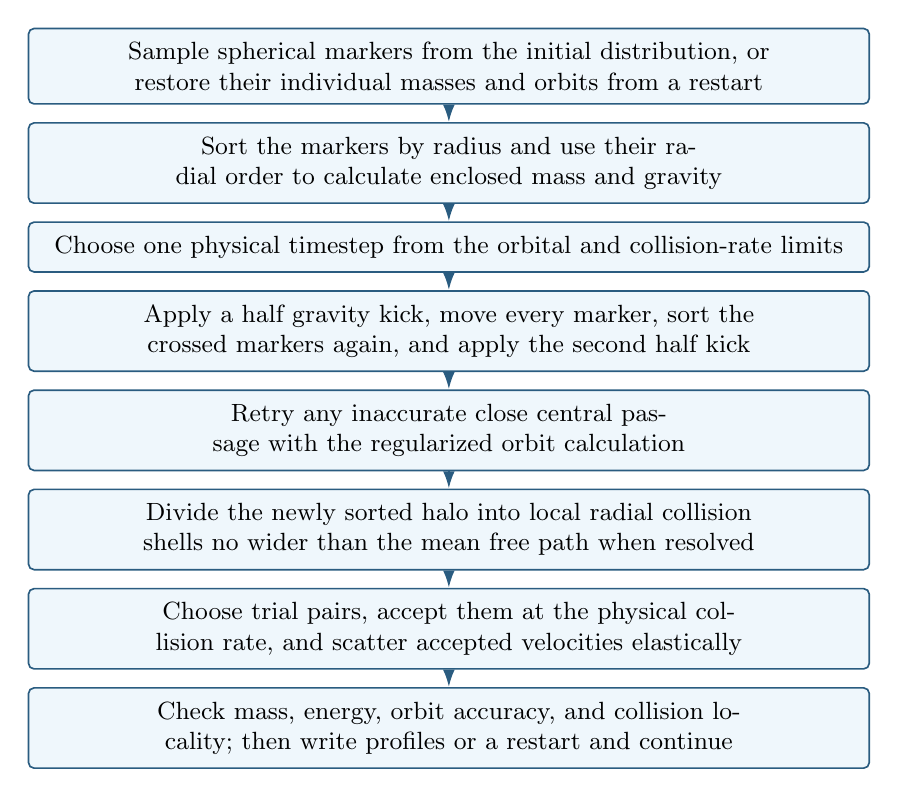
\begin{tikzpicture}[node distance=0.22cm]
\node[physicsflow] (sd1) {Sample spherical markers from the initial distribution, or restore their individual masses and orbits from a restart};
\node[physicsflow,below=of sd1] (sd2) {Sort the markers by radius and use their radial order to calculate enclosed mass and gravity};
\node[physicsflow,below=of sd2] (sd3) {Choose one physical timestep from the orbital and collision-rate limits};
\node[physicsflow,below=of sd3] (sd4) {Apply a half gravity kick, move every marker, sort the crossed markers again, and apply the second half kick};
\node[physicsflow,below=of sd4] (sd5) {Retry any inaccurate close central passage with the regularized orbit calculation};
\node[physicsflow,below=of sd5] (sd6) {Divide the newly sorted halo into local radial collision shells no wider than the mean free path when resolved};
\node[physicsflow,below=of sd6] (sd7) {Choose trial pairs, accept them at the physical collision rate, and scatter accepted velocities elastically};
\node[physicsflow,below=of sd7] (sd8) {Check mass, energy, orbit accuracy, and collision locality; then write profiles or a restart and continue};
\draw[physicsarrow] (sd1) -- (sd2);
\draw[physicsarrow] (sd2) -- (sd3);
\draw[physicsarrow] (sd3) -- (sd4);
\draw[physicsarrow] (sd4) -- (sd5);
\draw[physicsarrow] (sd5) -- (sd6);
\draw[physicsarrow] (sd6) -- (sd7);
\draw[physicsarrow] (sd7) -- (sd8);
\end{tikzpicture}
\end{figure}

\subsubsection{Purpose and physical picture}

SphDSMC solves the static Boltzmann--Poisson equations (PIC0b)--(PIC0c), with
\(H=0\), the full halo density as the Poisson source, and elastic binary
scattering in \(C[f]\).  It uses the same spherical phase space measure
(PIC0a).  The marker ordering supplies the enclosed mass directly, so the
force calculation implements the spherical Poisson equation without a
separate gravity mesh.  The orbital update and local collision sampling then
advance the two terms in the kinetic equation.

This solver represents the halo by a large set of computational
particles, called \emph{markers}.  Each marker keeps its radius, radial
velocity, angular momentum, and positive mass throughout the run.  A fresh
standard sample is equal mass, but the gravity, shell, collision, diagnostic,
and restart paths accept unequal masses.  Gravity moves the markers along
spherical orbits.  Collisions select nearby whole-object pairs and scatter
their continuous three-dimensional velocities.
An origin crossing is always reflected as
\(r\mapsto|r|\), \(v_r\mapsto-v_r\).  There is no outer wall: \code{r_max}
is the outer edge of the reported profile bins, not a reflecting boundary,
and a marker outside it remains part of the gravitational state.

It follows the SphDSMC construction of
\href{https://doi.org/10.1093/mnras/stag2015}{van den Bosch and Tokayer (2026)}.
The input \(f(r,w,L)\) supplies the probability distribution from which the
initial markers are drawn.  After this sampling step, the markers themselves
are the dynamical state.  The task selector and runnable interface are given
only after the state, gravity, timestep, and collision laws below.

One timestep proceeds as follows:
\begin{enumerate}
\item Sort the markers by radius and compute the spherical gravitational
      force from their radial order.
\item Apply half of the gravitational velocity kick.
\item Move every marker to its new radius.
\item Sort again, because markers may have crossed one another.
\item Apply the second half of the gravitational kick using the new radial
      order.
\item Divide the sorted markers into radial collision shells.
\item Draw the physical number of collision trials in each shell, accept
      pairs with the Boltzmann probability, and scatter every accepted pair.
\item Write profiles, conservation budgets, and restart data at their
      requested intervals.
\end{enumerate}

The orbit and output logic lives in
\path{cpu/include/ev/spherical_dsmc_solver.hpp}.  The pair-selection and
finite-angle scattering logic lives in
\path{cpu/include/ev/spherical_dsmc_collision.hpp}.

\subsubsection{How SphDSMC differs physically and numerically from WPIC}

The two modules approximate the same collisionless Vlasov--Poisson equation
between encounters, but their Vlasov updates are not identical numerical
algorithms.  In WPIC, unequal-weight markers deposit their mass onto a fixed
radial mesh; the spherical Poisson equation is solved on that mesh, and the
interpolated mesh force moves each marker.  In SphDSMC, the persistent markers
are sorted by their instantaneous radius, the actual marker masses are
prefix-summed in that order to obtain \(M(<r)\), and each marker receives the
corresponding spherical force directly.  SphDSMC therefore needs a stable
radius sort after every drift.  WPIC needs no radial sort for its gravity
solve, although its material-collision path may sort markers when constructing
adaptive collision shells.  Both use a time-centred kick--drift--kick orbit
update, so they solve the same physics while having different force noise,
spatial smoothing, and convergence errors.

Their elastic SIDM collision cores share the same physical ingredients:
local no-time-counter pair trials, the relative speed \(u\), a possibly
velocity-dependent pair area \(\Sigma_{ij}(u)\), and exact unequal-mass
centre-of-mass scattering.  ``No-time-counter'' means that trial pairs are
drawn from a safe rate bound rather than by advancing a separate clock for
every possible pair.  The complete SphDSMC pair remains two markers and the
present SphDSMC module has no inelastic capture channel.  Its collision
timestep is part of the one global physical timestep and elastic scattering
is applied once per accepted global step.

WPIC additionally has the Plummer-subhalo encounter operator.  It can either
scatter two complete unequal-mass subhalos or capture them into one remnant of
mass \(m_i+m_j\), placing the lost relative orbital kinetic energy into the
remnant's internal energy and velocity dispersion.  WPIC also separates the
ordinary Vlasov CFL timestep from the outer collision-operator deadline and
from the collision sampler's internal probability-limiting substeps.  Thus
the SphDSMC and WPIC collision laws can use the same elastic SIDM cross section,
but the calling cadence, collision-region construction, gravitational force
estimator, and available inelastic physics are not the same.

\subsubsection{Marker mass and initial sampling}

One marker stores
\codesource{SphDSMC marker state}
{\path{cpu/include/ev/spherical_dsmc_solver.hpp}}
{Defines the persistent radius, radial velocity, angular momentum, identifier,
 and represented mass carried by each spherical marker}
\begin{lstlisting}[language=C++,basicstyle=\ttfamily\scriptsize]
struct SphericalDSMCParticle {
    double r;
    double vr;
    double L;
    std::uint64_t id;
    double mass;
};
\end{lstlisting}
\code{SphericalDSMCParticle} is the C++ data record for one persistent
marker: it holds the marker's current phase space coordinates, immutable
integer identifier, and represented mass.  Here \(v_r\equiv w\), and
\[
 L=r v_t,\qquad v_t^2=v_\theta^2+v_\phi^2.
\]
The standard initializer gives every marker the same mass
\[
 m_p=\frac{M_{\rm represented}}{N_p}.
\]
Normally \(M_{\rm represented}\) is the integral of the carrier grid.  If the
source particle model supplies an independently known total mass,
\code{bp_dsmc_total_mass} sets that mass explicitly.  It changes only \(m_p\):
the normalized cumulative mass distribution, and therefore the sampled
phase space shape, stays fixed.

For a spherical distribution \(f(r,v_r,L)\), integration over position and
velocity angles gives
\[
 \dd M=8\pi^2 Lf(r,v_r,L)\,\dd r\,\dd v_r\,\dd L.
\]
Consequently, the piecewise-constant mass represented by one input cell is
\[
 \Delta M_{ijk}
 =8\pi^2L_k f_{ijk}\,
   \Delta r_i\,\Delta v_{r,j}\,\Delta L_k.                 \tag{S1}
\]
In equation (S1), \(i\), \(j\), and \(k\) index the radial,
radial-velocity, and angular momentum cells, respectively.  Elsewhere \(p\)
denotes an arbitrary marker, \(q=0,\ldots,N_p-1\) denotes its position in the
stratified initial sample, \(i\) denotes zero-based radial rank after sorting,
and \(s\) denotes a collision shell; each local use is stated explicitly.
The radial control-volume array has its innermost face at exactly \(r=0\).
The velocity and angular momentum widths are the same trapezoidal
control-volume widths used by the grid solver.

The code forms a cumulative table of the positive cell masses in (S1).
It then places \(N_p\) evenly spaced target masses along that table, using one
random offset \(\xi\in(0,1)\).  Marker \(q\) selects the cell containing
\[
 M_q=M_{\rm represented}\frac{q+\xi}{N_p},
 \qquad q=0,\ldots,N_p-1.
\]
This gives exactly \(N_p\) initially equal-mass markers and spreads the
selected cells evenly across the cumulative mass distribution.  The mass is
then stored on each marker.  Restart versions 4--7 preserve it individually;
collision code never infers equality from the initializer.

Within the selected cell, \(r\) and \(v_r\) are uniform.  Since the measure in
\(L\) is \(L\,\dd L=\tfrac12\dd(L^2)\), the sampler is uniform in \(L^2\):
\codesource{SphDSMC grid-to-marker sampler}
{\path{cpu/include/ev/spherical_dsmc_solver.hpp}}
{Samples continuous spherical phase coordinates from a selected positive-mass
 carrier cell, including the correct angular momentum measure}
\begin{lstlisting}[language=C++]
particle.r = r0 + (r1 - r0) * rng.uniform_open();
particle.vr = w0 + (w1 - w0) * rng.uniform_open();
particle.L = std::sqrt(
    L_lo * L_lo
    + (L_hi * L_hi - L_lo * L_lo) * rng.uniform_open());
\end{lstlisting}
The transformation from \(\dd^3x\,\dd^3v\) to
\(\dd r\,\dd v_r\,L\,\dd L\) cancels the radial \(r^2\) factor, yielding
uniform sampling in \(r\) inside the selected cell.

\subsubsection{Radius ordering, spherical force, and total energy}

The marker array is maintained in nondecreasing radius order.  For zero-based
radial rank \(i\), let \(m_i\) be that marker's mass, and let \(j<i\) denote
all strictly interior ranks.  The fixed central point mass is
\(M_\bullet=\code{central_mass}\); it is zero when no central object is
present.  The shell-centered enclosed force mass is
\[
 M_i^{\rm enc}=M_\bullet+\sum_{j<i}m_j+\frac12m_i.         \tag{S2}
\]
The characteristic equations are
\[
 \dot r_i=v_{r,i},\qquad
 \dot v_{r,i}=\frac{L_i^2}{r_i^3}
              -\frac{GM_i^{\rm enc}}{r_i^2},
 \qquad \dot L_i=0                                         \tag{S3}
\]
between collisions.

Equation (S2) is the spherical-shell analogue of centering a finite-volume
force in a mass cell.  The corresponding diagnostic kinetic and potential
energies are
\[
 K=\sum_i\frac{m_i}{2}
 \left(v_{r,i}^2+\frac{L_i^2}{r_i^2}\right),               \tag{S4}
\]
\[
 W=-G\sum_i\frac{m_iM_i^{\rm enc}}{r_i}.                  \tag{S5}
\]
The half-self contribution in (S5) is
\(-Gm_i^2/(2r_i)\) for the represented thin spherical shell and is consistent
with the centered force (S2).  The reported Newtonian virial ratio is
\(Q_{\rm vir}=2K/|W|\); values near one indicate global virial balance, but
this single scalar does not prove local equilibrium.

The ordinary update is kick--drift--sort--kick:
\codesource{SphDSMC gravity step}
{\path{cpu/include/ev/spherical_dsmc_solver.hpp}}
{Applies time-centred spherical gravity and rebuilds enclosed mass after marker
 crossings before the endpoint kick}
\begin{lstlisting}[language=C++]
particles[i].vr += 0.5 * dt
    * spherical_dsmc_acceleration(
          particles[i], enclosed_force_mass[i], p);
particles[i].r += dt * particles[i].vr;
spherical_dsmc_sort_particles(particles);
rebuild_enclosed_force_mass_from_sorted_marker_masses();
particles[i].vr += 0.5 * dt
    * spherical_dsmc_acceleration(
          particles[i], enclosed_force_mass[i], p);
\end{lstlisting}
The intermediate sort is physical: after shell crossings, the second kick
must use the new enclosed rank.  A one-thread paper-exact run uses Frank and
Tokayer's literal insertion pass after every evolved step.  A threaded
paper-exact run produces the same stable radial ordering with either that
literal pass or the stable block-and-merge decomposition described below.
Only the one-time initial ordering uses a general stable ordering method.
The generic VENUS path may use insertion, block-and-merge, or radix sorting
according to the measured disorder.

\paragraph{Insertion sort: repairing the order left by a small step.}
Insertion sort walks from the second marker to the end of the array.  At
position \(i\), it temporarily saves the marker as a \emph{key}, shifts every
preceding marker with radius larger than the key one place to the right, and
inserts the key into the empty position.  Equal radii are not shifted past one
another, so the ordering is \emph{stable}: markers with equal sort keys retain
their previous relative order.  In source form the essential operation is
\codesource{SphDSMC stable insertion sorter}
{\path{cpu/include/ev/spherical_dsmc_solver.hpp}}
{Repairs a nearly ordered radial marker range without changing the relative
 order of equal-radius markers}
\begin{lstlisting}[language=C++]
for (std::size_t i = begin + 1; i < end; ++i) {
    if (!(particles[i].r < particles[i - 1].r)) continue;
    SphericalDSMCParticle key = particles[i];
    std::size_t j = i;
    while (j > begin && key.r < particles[j - 1].r) {
        particles[j] = particles[j - 1];
        --j;
    }
    particles[j] = key;
}
\end{lstlisting}
For example, let the radius order after the drift be
\[
 [0.11_A,\;0.15_B,\;0.13_C,\;0.18_D].
\]
When \(C\) is the key, \(B\) moves one place to the right and \(C\) is
inserted before it:
\[
 [0.11_A,\;0.13_C,\;0.15_B,\;0.18_D].
\]
One \emph{inversion} is one out-of-order pair, such as \(B,C\) in this
example.  If the array has \(I\) inversions, insertion sort costs
\(O(N_p+I)\) operations and \(O(1)\) extra marker storage.  After a sufficiently
small physical timestep, most markers remain close to their former radial
rank, \(I\) is small, and insertion sort is almost linear.  Its worst case is
\(O(N_p^2)\), so it is inappropriate after broad radial disorder.

\paragraph{Threaded stable insertion-and-merge path.}
Paper-exact execution must reproduce the stable radial ordering generated by
Frank's insertion sort.  VENUS first counts adjacent inversions in parallel
and counts the 32-separated predicates
\[
 r_i<r_{i-32}\qquad (i\ge32).
\]
This second count is a probe for broad disorder; it is not a stored
measurement of how many ranks a particular marker moved.  With no adjacent
inversion, no sort is needed.  If at most \(N_p/4\) of the 32-separated
predicates are inverted, the paper-exact path applies the literal stable
insertion pass.  Above that threshold, the marker array is divided into
contiguous blocks.  Different threads insertion-sort different blocks, after
which successive stable merge levels combine blocks of width one, two, four,
and so on.  A scratch array holding \(N_p\) complete marker records is used
during the merge.  Choosing a marker from the left block when two radii are
equal preserves the same tie order as the serial stable sort.

For an evolved generic run, VENUS instead counts adjacent inversions.  At
most \(N_p/64\) adjacent inversions select insertion sort; a larger count
selects per-thread stable sorting of contiguous blocks followed by the same
stable merge tree.  A multi-thread initial sort uses radix sorting, while a
one-thread initial sort uses the standard stable general sort.  These
thresholds choose work, not physics: every branch returns the same
nondecreasing stable radius order needed by the force calculation.

\paragraph{Radix sort for a broadly disordered general run.}
A radix is the number of possible digits processed in one pass.  VENUS uses
radix 256, so one digit is one byte and there are 256 buckets.  A
\emph{bucket} is the consecutive output region assigned to one byte value.
All valid radii are finite and nonnegative; for such IEEE-754 double-precision
numbers, the unsigned 64-bit bit pattern has the same order as the numerical
radius.  The code therefore processes the eight bytes of the radius from
least significant to most significant.  Each byte pass is stable, so after
eight passes the complete 64-bit keys are in numerical order.

The parallel byte pass has four steps:
\begin{enumerate}
\item Divide the input into \(T\) consecutive thread chunks.  Thread \(t\)
      counts its byte values in a private histogram \(H_{td}\), where
      \(d=0,\ldots,255\).  A histogram is simply a table of counts.
\item Sum the thread histograms to obtain the total size of each bucket and
      its global starting position \(B_d\).
\item Give thread \(t\) its private starting offset
      \[
       O_{td}=B_d+\sum_{q<t}H_{qd}.
      \]
\item Each thread scans its own input chunk from left to right and writes a
      marker into its current \(O_{td}\), then increments that offset.
\end{enumerate}
The offsets assign disjoint output positions, so scattering requires no
atomic updates or locks.  Earlier input chunks receive earlier positions
inside every bucket, and each thread scans in input order; these two facts
make the parallel pass stable.

As a one-byte example, suppose two threads receive
\[
\begin{split}
 t=0 &: [13_A,2_B,13_C,5_D],\\
 t=1 &: [2_E,9_F,5_G,13_H].
\end{split}
\]
The nonzero local counts are
\[
\begin{array}{c|rrrr}
 &d=2&d=5&d=9&d=13\\ \hline
H_{0d}&1&1&0&2\\
H_{1d}&1&1&1&1
\end{array}
\]
and the global bucket starts are \(B_2=0\), \(B_5=2\), \(B_9=4\), and
\(B_{13}=5\).  Thread 0 therefore starts at positions
\((0,2,4,5)\); thread 1 starts at \((1,3,4,7)\).  Parallel scattering produces
\[
 [2_B,2_E,\;5_D,5_G,\;9_F,\;13_A,13_C,13_H],
\]
including the original order of equal keys.  The actual radius sorter repeats
this operation for all eight bytes:
\codesource{SphDSMC stable radix sorter}
{\path{cpu/include/ev/spherical_dsmc_solver.hpp}}
{Performs the general parallel stable radius ordering used for a broadly
 disordered or explicitly forced sort}
\begin{lstlisting}[language=C++]
for (int pass = 0; pass < 8; ++pass) {
    build_thread_private_histograms(pass);
    build_global_bucket_and_thread_offsets();
    parallel_stable_scatter(source, scratch, pass);
    std::swap(source, scratch);
}
\end{lstlisting}
Radix sorting costs \(O(8N_p)\) marker visits and one \(N_p\)-marker scratch
array.  Because it reads and writes the full 40-byte marker record eight
times, it is usually limited by memory bandwidth and is wasteful when only a
few crossings need repair.  The generic sorter therefore keeps insertion
sort for nearly ordered data.  Radix sorting can be forced for a benchmark
with \code{EV_SPHERICAL_DSMC_RADIX_SORT=1}; it is separate from the
paper-exact post-drift insertion rule.

\subsubsection{Physical global timestep}

The gravity timestep follows the SphDSMC dynamical criterion
\[
 \Delta t_{\rm grav}
 =\left[
 2\eta_{\rm grav}
 \min_i\left(\frac{r_i}{|a_{r,i}|}\right)
 \right]^{1/2},                                            \tag{S6}
\]
where \(\eta_{\rm grav}=\code{bp_dsmc_gravity_eta}\).  This supplies the orbit
accuracy criterion.

For collision shell \(s\), the code finds an upper bound
\({\cal K}_s\) on the physical pair kernel
\(u\Sigma_{ij}(u)\) for every possible marker pair in
that shell.  Collision-sampling literature calls such an upper bound a
\emph{majorant}.  Let
\[
 n_{{\rm partner},s}=\frac{N_s-1}{V_s}
\]
be the finite-shell density of possible partners for one selected marker.
The implemented collision limit is
\[
 \Delta t_{\rm coll}
 =\epsilon_{\rm coll}\min_s
 \begin{cases}
 \displaystyle
 \frac{4}{n_{{\rm partner},s}{\cal K}_s},
     &\text{paper-exact path},\\[1.1ex]
 \displaystyle
 \frac{1}{n_{{\rm partner},s}{\cal K}_s},
     &\text{generic path},
 \end{cases}                                               \tag{S7}
\]
Here
\(\epsilon_{\rm coll}=\code{bp_dsmc_collision_epsilon}\); its default is one.
For equal masses \(m_p\), a constant cross section per unit mass
\(s_\chi\), and the paper majorant, this becomes
\({\cal K}_s=4v_{\max,s}m_ps_\chi\), so the factor four cancels and
\[
 \Delta t_{\rm coll}
 =\epsilon_{\rm coll}
  \min_s\frac{1}{n_{{\rm partner},s}m_ps_\chi v_{\max,s}}.
\]
This is Frank and Tokayer's equation~(12), with the finite-\(N_s\) partner
density retained.  The \(4v_{\max}\) factor belongs to their trial-pair
majorant and must not shorten the paper collision timestep by another factor
of four.  The selected step is
\[
 \Delta t=\min\left(
 \Delta t_{\max},\Delta t_{\rm grav},\Delta t_{\rm coll},
 t_{\rm end}-t\right).                                     \tag{S8}
\]
Scattering is called once per physical global step.  The SphDSMC cadence is
therefore fixed by equations (S7)--(S8).

\subsubsection{Selective Levi--Civita orbit retry}

Very radial trajectories can have a pericentre timescale much shorter than
the global orbital time.  Near pericentre, the terms \(L^2/r^3\) and
\(GM/r^2\) can change rapidly during one ordinary step.

VENUS handles these markers through the following sequence:
\begin{enumerate}
\item Advance every marker with the ordinary kick--drift--kick step.
\item For each marker, compare the orbital energy before and after that step.
\item Accept the ordinary result when the relative energy change satisfies
      \code{vp_orbit_energy_tolerance}.
\item Return a failed marker to its original state and integrate the same
      interval in the regularized coordinate \(\varrho=\sqrt r\).
\item Accept the regularized result after its adaptive integrator converges
      and the energy check passes.
\end{enumerate}

The paper-exact energy criterion is Frank and Tokayer's full equation~(5).
For equal marker mass \(m_p\) and zero-based radial rank \(i\), it is
\[
 {\cal E}_i
 =\frac12v_{r,i}^2+\frac{L_i^2}{2r_i^2}
  -G\left[\frac{M_\bullet}{r_i}
  +m_p\left(\frac{i+1}{r_i}
  +\sum_{j=i+1}^{N_p-1}\frac1{r_j}\right)\right]. \tag{S9}
\]
The \(i+1\) term includes this marker's full spherical self contribution;
\(M_\bullet\) adds the configured central point mass.  The implementation
sums individual masses in both terms when the markers have unequal masses.
The full self-consistent energy of all markers is also tracked as a global
gravity diagnostic.

When the relative defect in (S9) exceeds
\code{vp_orbit_energy_tolerance}, the original marker is retraced using
\[
 \varrho=\sqrt r,\qquad \frac{\dd t}{\dd\tau}=r=\varrho^2. \tag{S10}
\]
For physical orbit equations
\((\dot r,\dot v_r)=F(r,v_r)\), the transformed system is
\[
 \frac{\dd\varrho}{\dd\tau}
   =\frac{\varrho}{2}\dot r,\qquad
 \frac{\dd v_r}{\dd\tau}=r\dot v_r,\qquad
 \frac{\dd t}{\dd\tau}=r.                                 \tag{S11}
\]
The paper-exact path integrates the transformed equations with
kick--drift--kick leapfrog steps in fictitious time, accumulates physical time
with the midpoint value of \(\varrho^2\), and linearly interpolates the final
overshooting step.  A failed equation~(S9) check repeats the original orbit
with the fictitious step halved.  The generic VENUS path retains its adaptive
Dormand--Prince integrator.

The retry is accepted only when the adaptive integrator converges and the
final defect in (S9) meets the requested tolerance.  The history reports the
numbers attempted, accepted,
unresolved, and failed inside the adaptive integrator, as well as the largest
ordinary and final energy defects.  A production result requires zero
unresolved retries.
\code{EV_SPHERICAL_DSMC_FORCE_CONSISTENT_ORBIT_AUDIT=1} is an opt-in
finite-\(N\) diagnostic: it subtracts the half-self term that is present in
the published equation-(5) audit potential but absent from the force used to
advance a marker.  It does not change that force, the published diagnostic,
the total energy, or any collision.  The resolved choice is recorded in
\path{metadata.json}.

\subsubsection{Adaptive radial collision shells and locality}

Collisions should pair markers that occupy the same local region.  The
generic execution path builds radial collision shells after the gravity update:
\begin{enumerate}
\item Start from the radius-sorted marker list.
\item Divide it into blocks containing approximately
      \code{bp_dsmc_shell_particles} markers.
\item Compute each block's radial width, density, evolving orbital velocity
      dispersion, and pair-rate-averaged mean free path.
\item Split a block in half when its width exceeds its mean free path and both
      children contain at least \code{bp_dsmc_min_shell_particles} markers.
\item Apply the same criterion recursively to the children.
\end{enumerate}

Paper-exact mode follows Frank and Tokayer's sequential shell construction.
At the first unused marker, it proposes the next target number of markers,
halves that candidate until its width is local or the population floor is
reached, accepts the shell, and advances to the next unused marker.  The next
candidate starts again at the target population.  The final candidate contains
the remaining consecutive markers, and the faces are their radial extrema,
as in their equation~(6).  Rebuilding either shell construction after gravity
uses the current marker positions.

\codesource{Paper-exact SphDSMC collision shells}
{\path{cpu/include/ev/spherical_dsmc_solver.hpp}}
{Shortened moving-cursor update; \code{describe} abbreviates the source's
 shell-description call, while \code{target} and \code{minimum} are the
 configured populations}
\begin{lstlisting}[language=C++]
while (begin < particles.size()) {
    std::size_t end = std::min(particles.size(), begin + target);
    auto shell = describe(begin, end);
    while (shell.outer_edge - shell.inner_edge > shell.mean_free_path
           && end - begin >= 2 * minimum) {
        end = begin + (end - begin) / 2;
        shell = describe(begin, end);
    }
    shells.push_back(shell);
    begin = end;
}
\end{lstlisting}

For shell edges \(r_{s,-},r_{s,+}\), marker count \(N_s\), and individual
marker masses \(m_i\),
\[
 V_s=\frac{4\pi}{3}(r_{s,+}^3-r_{s,-}^3),\qquad
 \rho_s=\frac{\sum_{i\in s}m_i}{V_s},\qquad
 n_s=\frac{N_s}{V_s},\qquad
 n_{{\rm partner},s}=\frac{N_s-1}{V_s},                    \tag{S12}
\]
\[
 \overline v_{r,s}=\frac{\sum_i m_i v_{r,i}}{\sum_i m_i},
 \qquad
 \sigma_{v,s}^{\,2}=
 \frac{\sum_i m_i[(v_{r,i}-\overline v_{r,s})^2+v_{t,i}^2]}
 {3\sum_i m_i},                                           \tag{S13a}
\]
\[
 \boxed{\displaystyle
 \lambda_s=
 \frac{\langle u_{ij}\rangle_s}
 {n_{{\rm partner},s}
  \langle u_{ij}\Sigma_{ij}(u_{ij})\rangle_s}}.             \tag{S13b}
\]
Here \(v_{r,i}\) and \(v_{t,i}=L_i/r_i\) are radial and tangential speed,
\(\overline v_{r,s}\) is the shell's mass-weighted radial drift,
\(\sigma_{v,s}\) is its one-dimensional orbital velocity dispersion,
\(u_{ij}\) is pair relative speed, and \(\Sigma_{ij}\) is the complete
unequal-mass physical pair area.  The density \(n_s\) estimates all objects,
whereas \(n_{{\rm partner},s}\) excludes the selected object itself; replacing
the latter by \(n_s\) is the large-\(N_s\) continuum approximation.  Angle
brackets average over unordered pairs and their unresolved relative
tangential azimuth.  VENUS uses all pairs when the shell contains at most 512
unordered pairs and otherwise uses 512 deterministic samples.  This
lets the evolving distribution function determine both the velocity scale
and a velocity-dependent cross section.  A single RMS-speed substitution is
not made.

For equal masses \(m_p\) and constant \(s_\chi=\sigma/m\),
\(\Sigma_{ij}=m_p s_\chi\), so equation (S13b) gives
\[
 \lambda_s=\frac{N_s}{N_s-1}\frac{1}{\rho_s s_\chi}.
\]
It approaches Frank and Tokayer's continuum expression
\(1/(\rho_s s_\chi)\) as \(N_s\) grows.  For an equal-mass,
constant-cross-section paper run, the code evaluates this finite-\(N_s\)
form directly.  The published Frank benchmark starts with equal masses, but
\code{EV_SPHERICAL_DSMC_PAPER_EXACT=1} does not reject an unequal-mass
restart.  In that case VENUS uses the unequal pair area and the sampled
velocity-dependent average in equation (S13b).  The shell, cadence,
remainder, and orbit conventions remain paper-exact; unequal masses are a
VENUS extension rather than a claim about the original benchmark.
The recursive decision in the source is
\codesource{SphDSMC adaptive collision-shell builder}
{\path{cpu/include/ev/spherical_dsmc_solver.hpp}}
{Bisects a radial collision region when its width exceeds the sampled physical
 mean free path and both child shells retain the minimum population}
\begin{lstlisting}[language=C++]
if (outer_edge - inner_edge > mean_free_path
    && size >= 2 * minimum) {
    split(begin, middle);
    split(middle, end);
}
\end{lstlisting}

After subdivision, VENUS targets
\[
 \Delta r_s\leq\lambda_s.                                  \tag{S14}
\]
Following Frank's SphDSMC algorithm, if the minimum marker population
prevents (S14), shell refinement stops at that population and the run
continues.  This is a spatial-resolution limit: collisions in such a shell
can transport heat too far.  The maximum \(\Delta r_s/\lambda_s\) and number
of violating shells are therefore written to \path{history.csv} and must be
compared with the resolved core size before late collapse is trusted.
Reduce the minimum population in a convergence sequence until the resolved
density and heat-flow profiles are insensitive to that choice.

\subsubsection{Equal-mass initial resolution at a target central density}
\label{sec:sphdsmc-marker-scaling}

Two length comparisons answer different physical questions.  The numerical
locality requirement is
\[
 \Delta r_{\rm coll}<\lambda_{\rm mfp},
\]
where \(\Delta r_{\rm coll}\) is the width of a collision shell.  Increasing
the marker resolution can improve this inequality.  The core Knudsen
condition is
\[
 r_{\rm core}<\lambda_{\rm mfp}.
\]
It states that the physical core is in the long-mean-free-path regime.
Changing the numerical marker count cannot change this second inequality.
SphDSMC can in principle describe a short-mean-free-path core,
\(\lambda_{\rm mfp}<r_{\rm core}\), but only if its collision shells remain
smaller than \(\lambda_{\rm mfp}\).  A conducting-fluid or kinetic--fluid
description becomes more economical when the core contains many mean free
paths.

The equal-mass resolution scaling follows from the innermost nearly uniform
core.  Let \(M\) be the total represented mass, \(N_p\) the global number of
equal-mass markers, and \(k\) the minimum population of the innermost
collision shell.  One marker represents
\[
 m_p=\frac{M}{N_p}.
\]
If the central shell has density \(\rho\) and characteristic radius
\(\Delta r\), its represented mass gives
\[
 k m_p\simeq \frac{4\pi}{3}\rho\,\Delta r^3,
 \qquad
 \Delta r\simeq
 \left(\frac{3kM}{4\pi N_p\rho}\right)^{1/3}.              \tag{S14a}
\]
Define the physical cross section per unit mass
\[
 s\equiv\frac{\sigma}{m},
 \qquad
 \lambda_{\rm mfp}=\frac{k}{k-1}\frac{1}{\rho s}.
\]
The second equality is the finite-\(k\) mean free path in the innermost
collision shell; \(1/(\rho s)\) is its continuum limit.
The locality ratio is therefore
\[
 \chi\equiv\frac{\Delta r}{\lambda_{\rm mfp}}
 \simeq
 \frac{k-1}{k}\,
 s\left(\frac{3kM}{4\pi N_p}\right)^{1/3}\rho^{2/3}.
                                                               \tag{S14b}
\]
Solving for the required global marker count gives
\[
 \boxed{
 N_{\rm req}\simeq
 \frac{3kM}{4\pi}\,
 \left(\frac{k-1}{k}\right)^3
 s^3\rho_{\rm target}^2\chi_{\rm target}^{-3}}
                                                               \tag{S14c}
\]
and hence the central result
\[
 N_{\rm req}\propto
 \frac{(k-1)^3}{k^2}
 \left(\frac{\sigma}{m}\right)^3\rho_{\rm target}^2
 \ \longrightarrow\
 k\left(\frac{\sigma}{m}\right)^3\rho_{\rm target}^2
 \quad(k\gg1).
                                                               \tag{S14d}
\]
Thus one additional decade in target density costs two decades in equal-mass
markers.  Doubling \(\sigma/m\) costs a factor \(2^3=8\).  In the continuum
approximation, lowering the minimum shell population from \(k=32\) to \(k=8\)
saves a factor of four in marker count and extends the density reach by a
factor of two.  Retaining the finite-\(k\) correction changes those factors
to about \(5.43\) and \(2.33\), respectively; this modest difference is
smaller than the need to demonstrate distribution-function convergence in a
shell containing only eight markers.
Demanding the safer margin \(\chi_{\rm target}=0.5\), rather than marginal
locality at \(\chi_{\rm target}=1\), costs another factor of eight.

\paragraph{Marker-count and memory planning.}
Equation (S14c) should be evaluated in the run's consistent unit system using
the target density, selected minimum shell population, and desired locality
margin.  For an equal-mass velocity-dependent model, the local effective
cross section per mass is
\[
 s_{\rm eff}=
 \frac{\langle u\,s(u)\rangle}{\langle u\rangle}.
\]
Using the largest locally relevant \(s(u)\) gives a conservative upper bound
for initial resource planning, while the evolving pair average in equation
(S13b) supplies the actual locality diagnostic.

The SphDSMC work arrays require approximately 180--210 bytes per marker: the
40-byte particle record is accompanied by energy, potential, rank,
shell-speed, collision-remainder, and sorting workspaces.  A useful estimate
is therefore
\[
 M_{\rm RAM}\simeq190N_p\ {
m bytes}.                    \tag{S14e}
\]
A version-6 restart has a 100-byte header and stores 40 bytes per marker;
paper-exact version 7 adds an 8-byte count and an 8-byte collision-remainder
record per marker.  The marker-count parameter is a 32-bit
integer and cannot exceed \(2.147\times10^9\).  SphDSMC uses one shared-memory
process rather than distributing markers over MPI ranks, so the complete
state and sorting workspace must fit on one node.  Runtime grows at least
linearly with marker count for transport and sorting, and the number of steps
also rises during collapse as the collision and orbital times shorten.

\subsubsection{Reconstructing local three-dimensional velocities}

At a radius, spherical symmetry stores only \(v_r\) and the tangential speed
\(v_t=L/r\); the tangential azimuth is uniformly distributed.  In the
paper-exact path a fresh azimuth \(\phi_i\) is sampled whenever a trial pair
is evaluated:
\[
 \bm v_i=(v_{r,i},v_{t,i}\cos\phi_i,v_{t,i}\sin\phi_i).
                                                               \tag{S15}
\]
In code,
\codesource{SphDSMC local velocity reconstruction}
{\path{cpu/include/ev/spherical_dsmc_solver.hpp}}
{Combines stored radial motion with a sampled tangential azimuth to recover a
 local three-dimensional velocity for a collision trial}
\begin{lstlisting}[language=C++]
velocities[local] = {
    particle.vr,
    vt * std::cos(angle),
    vt * std::sin(angle),
};
\end{lstlisting}
This is a continuous-velocity reconstruction, followed by direct assignment
of the post-collision marker velocity.

At \(r=0\), finite velocity requires \(L=0\) and the distribution is
isotropic. The stored radial departure speed is then the full speed.
Both collision samplers reconstruct an isotropic Cartesian direction there
and retain the outgoing magnitude after scattering. Their stored kinetic
energy therefore equals the conserved Cartesian kinetic energy. The
assignment is
\codesource{SphDSMC stored velocity after an elastic encounter}
{\path{cpu/include/ev/spherical_dsmc_solver.hpp}}
{Preserves the complete outgoing speed at the origin and the radial and
 angular components at positive radius}
\begin{lstlisting}[language=C++]
particle.vr = particle.r == 0.0
    ? std::hypot(velocity.x, std::hypot(velocity.y, velocity.z)) : velocity.x;
particle.L = particle.r * std::hypot(velocity.y, velocity.z);
\end{lstlisting}
The local dispersion gives zero mean projection and one-third of the squared
speed along any chosen axis at the origin. The positive-radius construction
in equation (S15) retains its radial and tangential meanings.

\subsubsection{Sampling the Boltzmann collision rate}

Consider one radial shell with \(N_s\) markers, volume \(V_s\), number
density \(n_s=N_s/V_s\), and possibly unequal marker masses.  The configured
material cross section per unit mass is
\[
 s_\chi(u)\equiv\frac{\sigma(u)}{m}.
\]
This notation applies to the \code{constant}, \code{powerlaw}, and
\code{yukawa_born} laws. The \path{softened_gravity} fit is a
physical-area model with a different unequal-mass scaling, given below.
A value of \(\sigma/m\) fixes the physical pair area only for the
single-species equal-mass problem.  It does not, by itself, derive a mixed
cross section for two different physical species.  The maintained
whole-object extension uses the explicit symmetric closure
\[
 \Sigma_{ij}(u)=\frac{m_i+m_j}{2}s_\chi(u),\qquad
 K_{ij}=u_{ij}\Sigma_{ij}(u_{ij}).                         \tag{S16a}
\]
This law is homogeneous under common refinement and recovers the configured
equal-mass area exactly.  Those two properties do not make it a
first-principles mixed-species interaction.  Production material-SIDM
benchmarks initialize equal masses and elastic scattering leaves them equal.
If \(m_i,m_j\) are distinct physical species, their microphysical
\(\Sigma_{ij}(u)\) must be supplied as additional physics.  If they are merely
unequal numerical sampling weights for one SIDM species, updating both whole
markers cannot simultaneously reproduce both weighted Boltzmann loss rates
and conserve represented pair momentum event by event; a dedicated weighted
DSMC construction is required.  VENUS does not silently claim otherwise.

Under the stated whole-object closure, neither partner is divided into
equal-mass packets.  The paper-exact pair-sampling algorithm is:
\begin{enumerate}
\item Bound every possible \(K_{ij}\) in the shell by \({\cal K}_s\).
      For a constant \(s_\chi\), the code uses
      \({\cal K}_s=4v_{\max,s}m_{\max,s}s_\chi\).
\item Compute the equation-(7) expected trial count and convert it to an
      integer using the persistent equation-(8) remainders.
\item Choose two distinct markers uniformly from the shell.
\item Give both markers fresh random tangential azimuths and compute their
      relative speed \(u_{ij}\).
\item Accept the pair with probability \(K_{ij}/{\cal K}_s\).
\item Scatter each accepted pair elastically in an isotropic outgoing
      direction.
\end{enumerate}

The upper bound is
\[
 {\cal K}_s\geq\max_{i,j}K_{ij},
 \qquad u_{ij}=|\bm v_i-\bm v_j|.                          \tag{S16b}
\]
The equation-(7) expected count is
\[
 \widehat N_{{\rm coll},s}
 =\binom{N_s}{2}\frac{{\cal K}_s\Delta t}{V_s}
 =\frac12(N_s-1)n_s{\cal K}_s\Delta t.                     \tag{S17}
\]
This is the physical unordered-pair count; self-pairs are excluded.  It
uses number density because each selected marker is a complete collision
partner.  Its mass enters through \(\Sigma_{ij}\), not through the pair
proposal probability.

Paper-exact execution uses \(\lfloor\widehat N_{{\rm coll},s}\rfloor\)
trials immediately.  Its fractional part is divided equally among the
shell's persistent particle accumulators \(A_i\).  When
\(\sum_{i\in s}A_i>1\), one extra trial is taken and \(1/N_s\) is subtracted
from every \(A_i\) in the shell.  The accumulators remain attached to
immutable particle IDs as particles change shells and are stored in
paper-exact restart format version 7.  A selected pair is accepted with
probability
\[
 P_{ij}=
 \frac{K_{ij}}{{\cal K}_s}.                                \tag{S18}
\]
For \(m_i=m_j\) and constant \(s_\chi\), this reduces exactly to
\(u_{ij}/(4v_{\max,s})\).
The generic non-paper VENUS path retains the exponential null-collision
clock and velocity-dependent analytic majorants described below.  It is not
used for the Frank benchmark.

Analytic majorants are used for every supported law.  For example,
\[
 s_\chi(u)=A s_0(u^2+u_0^2)^{-n/2}
\]
where \(A=\code{bp_collision_strength}\), \(s_0=\code{bp_sigma0}\),
\(u_0=\code{bp_sigma_u0}\), and \(n=\code{bp_sigma_n}\),
has the interior maximum of \(u s_\chi(u)\) at
\[
 u_*=\frac{u_0}{\sqrt{n-1}}\quad(n>1),                     \tag{S19}
\]
The Born-Yukawa cross section per mass is
\[
 s_{\chi,{\rm Y}}(u)=
 A\frac{4\pi\alpha_\chi^2m_\chi^2}
 {m_\phi^4[1+(m_\chi u/m_\phi)^2]}.                        \tag{S20}
\]
Here \(\alpha_\chi=\code{bp_yukawa_alpha}\),
\(m_\chi=\code{bp_yukawa_mchi}\), and
\(m_\phi=\code{bp_yukawa_mphi}\) are numerical input parameters.  Their
ratio sets a speed scale \(u_{\rm Y}=m_\phi/m_\chi\), and their amplitude
sets the zero-speed cross section per mass
\(s_0=4\pi\alpha_\chi^2m_\chi^2/m_\phi^4\).  Thus (S20) is
\(A s_0/[1+(u/u_{\rm Y})^2]\).  The material collision law interprets
this output in units of cross section per mass; \code{bp_sigma0} is unused
for this selection.  The conversion from a microscopic model is given below.
The product \(u s_{\chi,{\rm Y}}(u)\) has its maximum at
\(u_*=m_\phi/m_\chi\).
The constant, softened-gravity, and endpoint values are treated similarly.
If a sampled kernel exceeds its analytic majorant, the operator raises an
explicit error before applying collisions.

\paragraph{Converting a microscopic Yukawa model to material-SIDM inputs.}
\label{sec:yukawa-material-units}
In natural units \(\hbar=c=1\), let \(m_{\chi,{\rm phys}}\) and
\(m_{\phi,{\rm phys}}\) be the physical particle and mediator masses, and
let \(\alpha_{\rm phys}\) be their dimensionless coupling.  The Born
differential cross section is
\[
 \frac{\dd\sigma_{\rm phys}}{\dd\Omega}
 =\frac{\alpha_{\rm phys}^2m_{\chi,{\rm phys}}^2}
 {\left[m_{\phi,{\rm phys}}^2+
 \tfrac12m_{\chi,{\rm phys}}^2u^2(1-\mu)\right]^2},
 \qquad \mu=\cos\theta.                                  \tag{S20Y1}
\]
Here \(u\) is the relative speed in units of \(c\), and
\(y=(m_{\chi,{\rm phys}}u/m_{\phi,{\rm phys}})^2\) measures the angular
dependence of the scattering.  The zero-speed total cross section is
\(\sigma_0=4\pi\alpha_{\rm phys}^2m_{\chi,{\rm phys}}^2/
m_{\phi,{\rm phys}}^4\).  Integration over solid angle gives the total
cross section; weighting the same integral by \(1-\mu\) gives the
momentum-transfer cross section:
\[
 \sigma_{\rm tot}=\frac{\sigma_0}{1+y},\qquad
 \sigma_{\rm T}=\frac{2\sigma_0}{y^2}
       \left[\ln(1+y)-\frac{y}{1+y}\right].              \tag{S20Y2}
\]
Both approach \(\sigma_0\) as \(y\to0\).  The cross section per mass is
\(s_0=\sigma_0/m_{\chi,{\rm phys}}\), converted to the chosen physical
area and mass units before supplying a simulation input.

Let \(M_{\rm u}\), \(R_{\rm u}\), and \(V_{\rm u}\) be the simulation's
mass, length, and speed units.  The required numerical amplitude and speed are
\[
 s_{0,{\rm code}}=\frac{M_{\rm u}}{R_{\rm u}^2}s_{0,{\rm phys}},
 \qquad
 u_{{\rm Y},{\rm code}}=
 \frac{c}{V_{\rm u}}\frac{m_{\phi,{\rm phys}}}{m_{\chi,{\rm phys}}}.
                                                               \tag{S20Y3}
\]
Choose any positive numerical \(m_{\chi,{\rm code}}\), set
\(m_{\phi,{\rm code}}=u_{{\rm Y},{\rm code}}m_{\chi,{\rm code}}\),
and calibrate the input amplitude by
\[
 \alpha_{{\rm code}}=
 \left(\frac{s_{0,{\rm code}}m_{\phi,{\rm code}}^4}
 {4\pi m_{\chi,{\rm code}}^2}\right)^{1/2}.               \tag{S20Y4}
\]
Using these three numerical values in (S20) gives the intended physical
cross section per mass in native units.  The scattering angle uses the same
speed ratio.  The strength \(A\) then multiplies that calibrated law.
The Eulerian grid collision modules interpret their kernel output as an
area and require their own area normalization.

\codesource{Material-SIDM Yukawa parameter conversion}
{\path{cpu/include/ev/common.hpp};
 \path{cpu/include/ev/finite_angle_boltzmann.hpp}}
{Constructs the input amplitude and speed scale for equations (S20) and
 (S20Y3)--(S20Y4); \code{s0_code} and \code{u_y_code} are the converted
 physical inputs}
\begin{lstlisting}[language=C++]
p.bp_yukawa_mchi = 1.0;
p.bp_yukawa_mphi = u_y_code * p.bp_yukawa_mchi;
p.bp_yukawa_alpha = std::sqrt(
    s0_code * std::pow(p.bp_yukawa_mphi, 4)
    / (4.0 * PI * p.bp_yukawa_mchi * p.bp_yukawa_mchi));
p.bp_collision_strength = 1.0;
\end{lstlisting}

\paragraph{Unequal-mass softened-gravity area.}
The \code{softened_gravity} option is a saturated gravitational
momentum-transfer fit, not a material cross section per unit mass.  Let
\[
 m_{\rm ref}=\code{bp_subhalo_mass},\qquad
 a_{\rm ref}=\code{bp_subhalo_radius},\qquad
 \ln\Lambda=\code{bp_coulomb_log}.
\]
Here \(m_{\rm ref}\) and \(a_{\rm ref}\) are the reference subhalo mass and
radius, and \(\ln\Lambda\) is the Coulomb logarithm that represents the
resolved range of gravitational impact parameters.  Homologous constant-
density radii are
\[
 a_i=a_{\rm ref}\left(\frac{m_i}{m_{\rm ref}}\right)^{1/3},
 \qquad
 a_j=a_{\rm ref}\left(\frac{m_j}{m_{\rm ref}}\right)^{1/3},
 \qquad
 a_{ij}=\frac{a_i+a_j}{2}.                                \tag{S20a}
\]
The reference saturation area is
\[
 \Sigma_{{\rm sat},{\rm ref}}=
 \begin{cases}
 \code{bp_sigma0},&\code{bp_sigma0}>0,\\
 2\pi a_{\rm ref}^2,&\code{bp_sigma0}=0,
 \end{cases}
\]
and the unequal-pair saturation area is
\[
 \Sigma_{{\rm sat},ij}
 =\Sigma_{{\rm sat},{\rm ref}}
  \left(\frac{a_{ij}}{a_{\rm ref}}\right)^2.              \tag{S20b}
\]
Thus, only in this softened-gravity branch, a positive
\code{bp_sigma0} has dimensions of physical area rather than area per mass.
The high-speed gravitational amplitude and area are
\[
 C_{ij}=4\pi G^2m_{\rm ref}^2\ln\Lambda
 \left(\frac{m_i+m_j}{2m_{\rm ref}}\right)^2,\qquad
 \Sigma_{{\rm high},ij}(u)=\frac{C_{ij}}{u^4},            \tag{S20c}
\]
where \(G=\code{vp_gravity}\).  The final physical pair area is the harmonic
interpolation
\[
 \boxed{\displaystyle
 \Sigma_{ij}(u)=
 \frac{A}{
  \Sigma_{{\rm sat},ij}^{-1}
  +\Sigma_{{\rm high},ij}^{-1}(u)}} ,                    \tag{S20d}
\]
with \(A=\code{bp_collision_strength}\).  It approaches
\(A\Sigma_{{\rm sat},ij}\) at low speed and
\(A C_{ij}u^{-4}\) at high speed.  The associated outgoing direction is
sampled isotropically; this maintained option is a scalar transfer fit, not a
resolved gravitational deflection calculation.

\subsubsection{Elastic finite-angle scattering}

For an accepted incoming pair, define
\[
 M=m_1+m_2,\qquad
 \mu_{\rm red}=\frac{m_1m_2}{M},\qquad
 \bm V=\frac{m_1\bm v_1+m_2\bm v_2}{M},\qquad
 \bm u=\bm v_1-\bm v_2,\qquad u=|\bm u|.                   \tag{S21}
\]
After sampling an outgoing unit relative direction \(\hat{\bm n}\),
\[
 \bm v_1'=\bm V+\frac{m_2}{M}u\hat{\bm n},\qquad
 \bm v_2'=\bm V-\frac{m_1}{M}u\hat{\bm n}.                 \tag{S22}
\]
Equation (S22) conserves pair momentum and kinetic energy algebraically:
\[
 m_1\bm v_1'+m_2\bm v_2'
 =m_1\bm v_1+m_2\bm v_2,
\]
\[
 \frac12m_1v_1'^2+\frac12m_2v_2'^2
 =\frac12m_1v_1^2+\frac12m_2v_2^2.                        \tag{S23}
\]
The updated spherical variables are assigned directly:
\codesource{SphDSMC finite-angle collision update}
{\path{cpu/include/ev/spherical_dsmc_solver.hpp};
 \path{cpu/include/ev/spherical_dsmc_collision.hpp}}
{Maps the momentum- and energy-conserving outgoing three-dimensional velocity
 back to persistent radial velocity and angular momentum}
\begin{lstlisting}[language=C++]
particle.vr = velocities[local].x;
particle.L = particle.r * std::hypot(
    velocities[local].y,
    velocities[local].z);
\end{lstlisting}
Equation (S22) supplies the complete direct continuous-velocity update.

For constant, softened power-law, and softened-gravity total cross sections,
the outgoing relative direction is isotropic.  For Born-Yukawa scattering,
\[
 \frac{\dd\sigma}{\dd\Omega}
 =A\frac{\alpha_\chi^2m_\chi^2}
 {\left[
 m_\phi^2+\tfrac12m_\chi^2u^2(1-\mu)
 \right]^2},\qquad \mu=\cos\theta.                         \tag{S24}
\]
The code analytically inverts the cumulative probability in \(\mu\) and
samples the scattering azimuth uniformly.  Integrating (S24) over
\(2\pi\,\dd\mu\) gives (S20), fixing the differential-to-total normalization
used by the sampler.

\subsubsection{Maxwellian equilibrium}

At equilibrium, every collision channel has the same probability as its
reverse channel.  This equality of forward and reverse rates is called
detailed balance.  It follows directly from elastic pair conservation.

For equal masses with common mean velocity \(\bm U\) and one-component
velocity variance \(T\),
\[
 f_M(\bm v)\propto
 \exp\left[-\frac{|\bm v-\bm U|^2}{2T}\right],
\]
pair momentum and kinetic-energy conservation imply
\[
 f_M(\bm v_1)f_M(\bm v_2)
 =f_M(\bm v_1')f_M(\bm v_2').                              \tag{S25}
\]
Reversing the outgoing relative direction in (S22) recovers the incoming
pair, and equations (S17)--(S18) sample the physical factor
\(u\,\dd\sigma/\dd\Omega\).  Detailed balance therefore makes the
equal-mass Maxwellian an exact stationary distribution of the underlying
continuous collision process.  For unequal physical object masses, the
equilibrium product instead uses the mass-weighted exponent derived after
(PIC35M), with a common thermodynamic temperature.
The finite-marker realization fluctuates statistically, but its ensemble
residual decreases with \(N_p\).

For a quantitative equilibrium reference, consider \(N\) equal-mass markers
of mass \(m_p\) in volume \(V\).  Define
\[
 n=\frac{N}{V},\qquad
 n_{\rm partner}=\frac{N-1}{V},\qquad
 \rho=nm_p,\qquad
 \Sigma_0=m_ps_0 ,
\]
where \(s_0=\sigma/m\) is the constant cross section per unit mass and
\(\Sigma_0\) is the physical pair area.  The analytic accepted-event rate per
volume is
\[
 {\cal R}_{\rm event}
 =\frac12 n\,n_{\rm partner}\Sigma_0\langle u\rangle
 =\frac12\frac{\rho^2s_0}{m_p}
  \left(1-\frac1N\right)\langle u\rangle,\qquad
 \left\langle u\right\rangle=4\sqrt{\frac{T}{\pi}}.         \tag{S26}
\]
Here \(T\) is the variance of each Cartesian velocity component in equation
(S25).  The factor \(1-1/N\) is the exact finite-ensemble exclusion of
self-pairs.  The sampled rate should approach equation (S26) within its
Monte--Carlo uncertainty, and independent realizations at successively larger
\(N_p\) should show the expected \(N_p^{-1/2}\) decrease of the velocity-
histogram fluctuation.  A fixed numerical value from one random ensemble is
not a physical calibration.

\subsubsection{Conservation ledgers}

Each persistent marker carries its own fixed represented mass throughout the
elastic SphDSMC run.  Every operator step writes explicit before/after
mass-weighted budgets to
\path{operator_mass_budget.csv}.  The fields include
\begin{itemize}[itemsep=0.25em]
\item transport mass and full energy before and after gravity;

\item collision mass before and after scattering;

\item collision radial momentum before and after scattering;

\item collision kinetic energy before and after scattering;

\item maximum pair-level momentum and kinetic-energy residuals.
\end{itemize}
The stored global spherical observables are radial momentum and full pair
kinetic energy.  The tangential azimuth in (S15) supplies an auxiliary local
realization.

The collision step must preserve marker mass exactly, and its mass-weighted
pair momentum and kinetic energy must close to floating-point roundoff.
Transport energy is an integration diagnostic rather than an exact
kick--drift--kick invariant; it must converge as the gravity timestep is
reduced.  A physically interpreted run additionally requires
\(\max_s\Delta r_s/\lambda_s<1\) and zero unresolved LC retries.  These
requirements belong to every run and are not replaced by one stored benchmark
number.

\subsubsection{Initial-condition provenance and acceptance checks}

The consuming constant-law task is
\code{venus_cpu_sidm_sphdsmc_constant}, selected by
\path{cpu/src/apps/sidm/sphdsmc_constant.cpp}.  In the grid-backed route,
\code{read_initial_data_rwl} in \path{cpu/include/ev/initial_data.hpp} imports
an \code{EVICRWL1} object such as
\path{cpu/examples/initial_data/frank_core_eq2_r1e3_model1e6_originlinear_Nr64_Nw32_NL40.bin}.
\code{EVICRWL1} is the bounded magic identifier at the start of a versioned
binary carrier containing the \((r,w,L)\) coordinate grids and the sampled
distribution array \(f(r,w,L)\); it is a file format, not an evolution
variable.  Then \code{spherical_dsmc_sample_initial_particles} in
\path{cpu/include/ev/spherical_dsmc_solver.hpp} samples the in-memory
\code{std::vector<SphericalDSMCParticle>} that becomes the dynamical state.
This C++ object is a contiguous variable-length list of the marker records
defined above.

The solver writes \code{VENUSSPHDSMC1} restart objects beneath the configured
\path{restart_dir}.  \code{VENUSSPHDSMC1} is the bounded magic identifier for
the versioned SphDSMC checkpoint format; the checkpoint contains evolution
time and step metadata together with the persistent marker state and the
version-specific deterministic collision remainder data.
A direct marker route is provided by
\path{cpu/tools/generate_frank_core_spherical_dsmc_restart.py}.  That generator
writes the same \code{VENUSSPHDSMC1} object consumed through
\code{--restart-from}, bypassing carrier-grid sampling.

Whichever route is used, validate the file identifier and version, finite
positive individual masses, unique identifiers, total represented mass,
radial support, the virial ratio \(Q_{\rm vir}=2K/|W|\), energy diagnostics,
initial equilibrium drift, collision-shell occupancy, and mean-free-path
locality.  Repeat the calculation under marker, seed, and timestep refinement;
agreement of one generated state is not a convergence test.

\subsubsection{Restart format and determinism}

SphDSMC restart formats 6 and 7 store each marker's radius, radial velocity,
angular momentum, ID, and individual mass as fixed-width native binary values.
Their header also stores the next collision timestep and a fingerprint of
the collision settings that generated it.  Version 7 includes the per-particle
integer+remainder state used by paper-exact collisions.

The next collision limit is part of the evolving numerical state.  After a
collision stage, the solver computes this limit from that stage's shell
geometry and retained pair-kernel majorants.  A fresh shell reconstruction
from the scattered particles can give a different limit, particularly when
paper-exact scattering changes the largest speed.  Restoring the stored
limit therefore preserves the next accepted timestep.  The implementation
selects the stored value before it enters the timestep loop:
\codesource{SphDSMC collision-clock restoration}
{\path{cpu/include/ev/spherical_dsmc_solver.hpp}}
{Restores the carried collision timestep and reconstructs an initial limit
 for a fresh ensemble or a legacy checkpoint}
\begin{lstlisting}[language=C++]
if (restored_collision_dt.has_value()) {
    next_collision_dt = restored_collision_dt.value();
} else {
    const std::vector<SphericalDSMCShell> initial_shells =
        spherical_dsmc_build_shells(
            particles, particle_mass, state.global_p,
            timestep_shell_workspace);
    next_collision_dt = spherical_dsmc_collision_timestep(
        initial_shells, state.global_p);
    if (restart_input_version != 0) {
        std::cout << "spherical_dsmc legacy restart version="
                  << restart_input_version
                  << " has no persisted collision clock; "
                     "reconstructing the first collision limit\n";
    }
}
\end{lstlisting}
The fingerprint checks the cross-section law and its parameters, angular
kernel, collision strength, shell target and floor, collision timestep
fraction, random seed, and collision mode.  It also includes the gravitational
constant used by the softened-gravity pair law.  Changing these settings
requires a separately initialized physical case; an exact continuation
rejects a mismatched clock.  An infinite positive limit represents an
inactive collision constraint.

Legacy versions 2--5 remain readable.  Versions 2 and 3 copy their common
header mass onto every restored marker; versions 4 and 5 already store
individual masses.  These legacy files initialize the first collision limit
from the restored ensemble, and metadata records this reconstruction.  Their
subsequent checkpoints use the complete current state.  This import preserves
the stored physical ensemble and the available fractional remainders; exact
reproduction of the missing historical collision clock requires a current
checkpoint.

The reader validates the bounded magic identifier, supported version,
nonnegative finite time and safely representable step, initial energy and
counters, positive finite masses, finite coordinates, nonnegative \(L\), and
the uniqueness and range of all stable marker IDs.  Before allocating the
particle vector, it proves that the count fits the version-specific payload.
The complete payload must end after its declared particle and remainder
records, and a stored collision limit must be positive and non-NaN.
Because the writer does not canonicalize byte order or floating-point
representation, move a checkpoint between machines only when their binary
representations are compatible; the CSV diagnostics are the portable
exchange format.

The checkpoint is first written to a temporary file and atomically renamed.
The random streams are deterministic functions of the base seed, global step,
and shell index.  With unchanged physical and numerical settings,
continuation at a natural step boundary preserves the stored stochastic
state, collision clock, and marker ordering.  The actual-solver regression
compares six uninterrupted steps with a three-step run followed by three
resumed steps in both collision modes, including accepted collisions and the
complete final checkpoint.

\subsubsection{Shared-memory organization and computational scaling}

The module requires one process:
\codesource{SphDSMC process-layout contract}
{\path{cpu/Makefile}; \path{cpu/include/ev/parallel.hpp};
 \path{cpu/include/ev/spherical_dsmc_solver.hpp}}
{Documents the enforced one-process execution model and assigns parallel work
 to portable C++ threads or OpenMP threads inside that process}
\begin{lstlisting}
#SBATCH --ntasks=1
#SBATCH --cpus-per-task=<OpenMP threads>
export OMP_NUM_THREADS=$SLURM_CPUS_PER_TASK
\end{lstlisting}
The unsuffixed executable uses the portable C++ \code{std::thread} backend;
the \code{_openmp} executable uses OpenMP.  Both run as one process.  Gravity
loops are parallel over markers.  Collision shells are disjoint and
dynamically scheduled over the selected thread backend, giving each marker
one thread owner during a shell update.

The stochastic work is proportional to the number of physically sampled NTC
trials.  Each accepted event realizes one continuous outgoing angle and
directly updates its two markers.  Marker drifts, force evaluations, profile
deposition, inversion counting, radix histograms, and independent collision
shells are parallel.  The stable radius merge, enclosed-mass prefix work,
suffix potential, and memory movement contain serial or memory-bandwidth
limits, so doubling the thread count need not halve the elapsed time.  For
\(N_p\) markers, state and sorting scratch require \(O(N_p)\) memory, while
one ordinary step costs \(O(N_p+N_{\rm trial})\) after sorting, where
\(N_{\rm trial}\) is the NTC trial count.  Measure a short fixed-work
strong-scaling run at 1, 2, 4, 8, 16, and 32 threads on the target machine and
choose the smallest allocation beyond which the elapsed time changes little.

\subsubsection{Configuration block}

A constant-cross-section SphDSMC run begins with the task selectors, physical
controls, initial-data source, time limits, input/output (I/O) paths, and
thread count below:
\codesource{\code{venus_cpu_sidm_sphdsmc_constant}}
{\path{cpu/src/apps/sidm/sphdsmc_constant.cpp};
 \path{cpu/include/ev/config.hpp}}
{Parses the explicit constant-law SphDSMC configuration and rejects task-
 incompatible physics selections}
\begin{lstlisting}
[physics]
physics_model = boltzmann_poisson
vp_universe = static
vp_gravity = 1
vp_poisson_source = total_density
vp_orbit_regularization = auto
vp_orbit_energy_tolerance = 0.01
vp_orbit_lc_relative_tolerance = 1e-9
vp_orbit_lc_absolute_tolerance = 1e-12
vp_orbit_lc_max_steps = 2048
vp_orbit_lc_max_refinements = 20

[collisions]
bp_collision_operator = spherical_dsmc
bp_cross_section = constant
bp_boltzmann_kernel = isotropic
bp_collision_strength = 1
bp_sigma0 = 1
bp_dsmc_particles = 1000000
bp_dsmc_total_mass = 1.1252580933331495
bp_dsmc_shell_particles = 4096
bp_dsmc_min_shell_particles = 32
bp_dsmc_collision_epsilon = 1
bp_dsmc_gravity_eta = 0.01
bp_dsmc_seed = 5489

[initial_data]
initial_data = binary_rwl
initial_data_file = examples/initial_data/frank_core_eq2_r1e3_model1e6_originlinear_Nr64_Nw32_NL40.bin
custom_ic_normalize_mass = false

[time_integration]
integrator = semi_lagrangian_kick_drift_kick
t_end = 0.05
dt_max = 0.01
max_steps = 1000000

[output]
output_dir = output/spherical_dsmc_example
restart_dir = output/spherical_dsmc_example/restarts
save_every = 1
phase_every = 0
restart_every = 5

[parallelism]
threads = 8
\end{lstlisting}
Because this example selects \code{bp_cross_section = constant},
\code{bp_sigma0} is interpreted as cross section per unit mass in the chosen
code units, so the continuum local rate is \(\rho u(\sigma/m)\).  The value
one above is a runnable dimensionless example.  For
\code{bp_cross_section = softened_gravity}, however, a positive
\code{bp_sigma0} is the physical reference saturation area in equation
(S20b), not a cross section per mass.  A literature benchmark must convert
its quoted cross section, density, velocity, length, and time into one
consistent unit system before replacing these values.

Build the constant-cross-section task frontend and run the parameter file from
the CPU source directory:
\codesource{\code{venus_cpu_sidm_sphdsmc_constant}}
{\path{cpu/src/apps/sidm/sphdsmc_constant.cpp};
 \path{cpu/Makefile}}
{Builds and runs the fail-closed constant-isotropic SphDSMC task frontend}
\begin{lstlisting}[basicstyle=\ttfamily\scriptsize]
cd VENUS/cpu
make venus_cpu_sidm_sphdsmc_constant
./venus_cpu_sidm_sphdsmc_constant --config params.ini
\end{lstlisting}
The executable's \code{--help} interface lists the collision, orbit, shell
and restart controls. A fresh calculation reads its initial distribution;
a continuation reads the complete persistent-marker restart. The physical
SIDM demonstrations and saved profiles are described in \path{analysis/README.md}.

\subsubsection{Convergence requirements}

A gravothermal-collapse calculation requires a joint refinement of the
marker, orbit, collision, and output scales:
\begin{enumerate}
\item increase the marker count by factors of two and compare density,
velocity dispersion, heat flux, collision rate, and core radius;
\item halve \(\epsilon_{\rm coll}\), the gravity parameter, and the target
shell population independently, then jointly;
\item require pair momentum and kinetic energy to close to floating-point
accuracy, transport energy error to decrease with timestep, all orbit retries
to resolve, and \(\Delta r_s/\lambda_s<1\) in every collision shell;
\item compare constant and velocity-dependent kernels with equation (S26),
detailed balance, the analytic majorants, and the Yukawa differential-to-total
normalization where applicable;
\item compare uninterrupted and restarted evolution at a natural step
boundary and repeat stochastic profile comparisons with independent seeds;
\item compare with the selected literature density profile through the
      full quoted dimensionless time;
\item follow a constant-cross-section Plummer core-formation and core-collapse
      sequence with the same unit conversion and boundary convention.
\end{enumerate}


\section{Einstein--Vlasov in Schwarzschild and Ingoing EF Coordinates}

The next two chapters describe the same relativistic collisionless matter in
two coordinate systems.  The Schwarzschild formulation provides the exterior
reference and the ingoing Eddington--Finkelstein (EF) formulation supplies the
horizon-penetrating evolution.  Coordinate comparison always identifies the
same spacetime event before comparing fields or markers.

\ifvenusfullcpu
\subsection{Weighted Einstein--Vlasov Particle--Mesh Module}
\label{sec:weighted-einstein-vlasov-pic}

This collisionless module evolves a spherical relativistic marker ensemble
and its self-consistent spacetime in Schwarzschild coordinates.  Separate task
executables select a low-compactness halo or high-compactness collapse, so a
parameter file cannot silently switch between those physical problems.  The
module contains no SIDM collision operator and does not evolve an expanding
cosmological background.  Schwarzschild coordinates approach a coordinate
singularity as \(2m/r\rightarrow1\); the module therefore diagnoses horizon
approach but is not a horizon-penetrating black-hole evolution scheme.

\noindent\textbf{Maturity and validation.}
The task-specific runners implement the Schwarzschild weighted
particle-in-cell (WPIC) method.  The low-compactness task compares
Einstein--Vlasov and Vlasov--Poisson evolution from the same sampled initial
positions and momenta.  Each module assigns the weights required by its own
phase-space measure.  Quantitative collapse results require joint refinement
of marker number, radial mesh, timestep, omitted-weight control, and sampling
realization, together with constraint, mass, binding, and outcome checks.
Horizon-penetrating evolution belongs to the EF module.

\begin{figure}[htbp]
\centering
\textbf{Physics flow: Einstein--Vlasov WPIC}
\par\smallskip
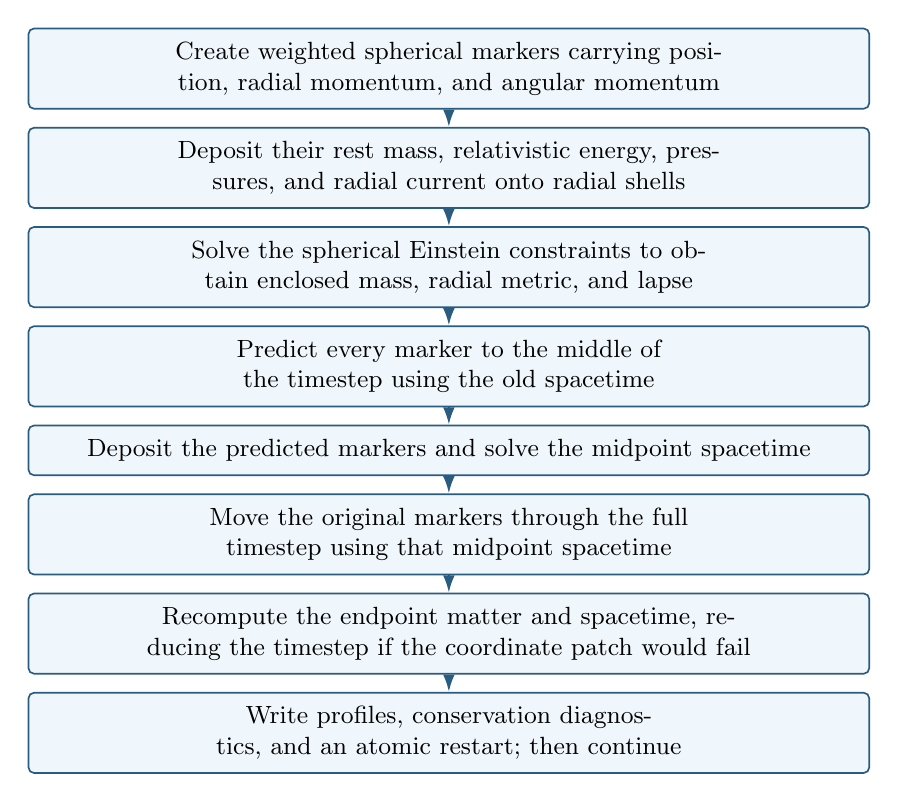
\begin{tikzpicture}[node distance=0.22cm]
\node[physicsflow] (ew1) {Create weighted spherical markers carrying position, radial momentum, and angular momentum};
\node[physicsflow,below=of ew1] (ew2) {Deposit their rest mass, relativistic energy, pressures, and radial current onto radial shells};
\node[physicsflow,below=of ew2] (ew3) {Solve the spherical Einstein constraints to obtain enclosed mass, radial metric, and lapse};
\node[physicsflow,below=of ew3] (ew4) {Predict every marker to the middle of the timestep using the old spacetime};
\node[physicsflow,below=of ew4] (ew5) {Deposit the predicted markers and solve the midpoint spacetime};
\node[physicsflow,below=of ew5] (ew6) {Move the original markers through the full timestep using that midpoint spacetime};
\node[physicsflow,below=of ew6] (ew7) {Recompute the endpoint matter and spacetime, reducing the timestep if the coordinate patch would fail};
\node[physicsflow,below=of ew7] (ew8) {Write profiles, conservation diagnostics, and an atomic restart; then continue};
\draw[physicsarrow] (ew1) -- (ew2);
\draw[physicsarrow] (ew2) -- (ew3);
\draw[physicsarrow] (ew3) -- (ew4);
\draw[physicsarrow] (ew4) -- (ew5);
\draw[physicsarrow] (ew5) -- (ew6);
\draw[physicsarrow] (ew6) -- (ew7);
\draw[physicsarrow] (ew7) -- (ew8);
\end{tikzpicture}
\end{figure}

\subsubsection{Physical variables and invariant marker weight}

The Schwarzschild line element is
\[
 \dd s^2=-e^{2\mu(\tau,r)}\dd\tau^2
          +e^{2\lambda(\tau,r)}\dd r^2+r^2\dd\Omega^2,    \tag{EWP1}
\]
where \(r\) is areal radius, \(\tau\) is Schwarzschild coordinate time,
\(\mu\) is the lapse
potential, \(\lambda\) is the radial metric potential, and
\(\dd\Omega^2\) is the unit-sphere metric.  In the source,
\code{WeightedPICMarker} is the record for one persistent numerical sample of
the distribution.  A marker stores
\[
 (m_p,r_p,w_p,\eta_p,I_p),\qquad
 \eta_p=\frac{L_p^2}{2},\qquad
 \epsilon_p=\sqrt{1+w_p^2+\frac{2\eta_p}{r_p^2}}.        \tag{EWP2}
\]
Here \(m_p\) is invariant rest-number weight, \(w_p\) is orthonormal radial
momentum measured by a local static observer, \(L_p\) is the conserved
angular-momentum magnitude, \(I_p\) is a persistent identifier, and
\(\epsilon_p\) is energy per unit rest mass in that local orthonormal frame.

Because \(w\) is orthonormal rather than canonical, the invariant reduced
phase measure is
\[
 \dd\Gamma_{\rm inv}
 =8\pi^2 e^\lambda\,\dd r\,\dd w\,\dd\eta.               \tag{EWP3}
\]
An initial sampler first constructs coordinate weights using
\(\dd r\,\dd w\,\dd\eta\), then iterates
\[
 m_p^{(n+1)}
 =m_{p,\rm coord}\exp[\lambda^{(n)}(r_p)]                \tag{EWP4}
\]
until the relative change is below \(2\times10^{-12}\).  This fixed-point
iteration makes \(m_p\) the invariant weight required by equation (EWP3).
This metric factor converts coordinate-volume sampling into invariant
particle number.  Omitting it changes the matter source and produces a false
growth of Arnowitt--Deser--Misner (ADM) mass, the total gravitating mass read
from the asymptotic exterior metric.

There is one explicit interface exception.  Markers returned by
\path{cpu/include/ev/weighted_einstein_vlasov_static_shell.hpp} already carry the
fully invariant quadrature weight.  For its continuum distribution
\(f=C(1-E/E_0)_+^k\delta(L-L_0)\), \(C\) is the distribution amplitude,
\(L_0>0\) is the single angular-momentum magnitude carried by the shell,
\((x)_+=\max(x,0)\) keeps only the positive part, and \(\delta\) is the Dirac
delta distribution that enforces \(L=L_0\).
The cutoff power satisfies \(1\le k\le8\), with default \(k=1\).
\(E_p=e^{\mu(r_p)}\epsilon_p\) is marker \(p\)'s conserved energy in the
static metric, and \(E_0\) is the upper energy cutoff.  The factors
\(\Delta r_p\) and \(\Delta w_p\) are the radial and positive-radial-momentum
quadrature measures assigned to that sample; each includes its numerical
quadrature weight rather than denoting a universal mesh spacing.  The returned
marker weight is
\[
 m_p=8\pi^2 CL_0 e^{\lambda(r_p)}
      \left(1-\frac{E_p}{E_0}\right)^k
      \Delta r_p\,\Delta w_p .
\]
The \code{energy_cutoff_shell} driver therefore passes those weights directly
to the Schwarzschild WPIC solver and must \emph{not} call
\code{canonicalize_weighted_einstein_vlasov_pic_initial_weights};
doing so would insert \(e^\lambda\) twice.  Its exact continuum equations,
delta-function normalization, sampling rules, fixed inward perturbation, and
threshold interface are documented in
Section~\ref{sec:ef-static-energy-cutoff-shell}.

\subsubsection{Relativistic deposition}

Markers deposit into shell centers placed uniformly in the volume coordinate
\[
 q=\frac{r^3}{3},\qquad \Delta V_i=4\pi\Delta q_i.       \tag{EWP5}
\]
CIC means cloud in cell, a two-center linear particle shape; TSC means
triangular shaped cloud, a smoother three-center quadratic shape.  TSC is the
default.  Let \(a_{pi}\) be the nonnegative shape weight of marker \(p\) in
shell \(i\), with \(\sum_i a_{pi}=1\).  The deposited shell-extensive
quantities are
\[
\begin{aligned}
 {\cal M}_{0,i}&=\sum_p a_{pi}m_p,\\
 {\cal E}_i&=\sum_p a_{pi}m_p\epsilon_p,\\
 {\cal P}_{r,i}&=\sum_p a_{pi}m_p\frac{w_p^2}{\epsilon_p},\\
 {\cal P}_{t,i}&=\sum_p a_{pi}m_p
                 \frac{2\eta_p/r_p^2}{\epsilon_p},\\
 {\cal J}_i&=\sum_p a_{pi}m_pw_p.
\end{aligned}                                           \tag{EWP6}
\]
\({\cal M}_0\) is rest mass, \({\cal E}\) is the invariant-weighted local
particle energy, the two
\({\cal P}\)'s generate radial and tangential pressure, and \({\cal J}\) is
radial current.  Unequal-weight sampling quality is reported by
\[
 N_{{\rm eff},i}
 =\frac{(\sum_p a_{pi}m_p)^2}{\sum_p(a_{pi}m_p)^2}.      \tag{EWP7}
\]

\subsubsection{Einstein constraint solve}

Define the metric gap
\[
 g(r)=1-\frac{2m(r)}{r}=e^{-2\lambda(r)},                \tag{EWP8}
\]
where \(m(r)\) is the Misner--Sharp enclosed mass.  Inside one shell, the
source \({\cal E}_i/\Delta q_i\) is held constant and the radial mass
constraint is integrated directly:
\[
 \frac{\dd m}{\dd q}
 =\frac{{\cal E}_i}{\Delta q_i}
  \sqrt{1-\frac{2m}{r(q)}}.                              \tag{EWP9}
\]
The square root is the \(e^{-\lambda}\) conversion from invariant canonical
marker measure to physical stress energy.  VENUS uses an implicit-midpoint
step with step doubling.  A radial segment is never accepted if its outer
face has \(2m/r\ge1\); this is a coordinate-patch condition, not an artificial
density cap.

For a radial segment \([q_L,q_R]\), write \(m_L=m(q_L)\),
\(r_m=[3(q_L+q_R)/2]^{1/3}\), and
\(Q=({\cal E}_i/\Delta q_i)(q_R-q_L)\).  The implicit-midpoint equation
for the mass increment \(\delta m=m_R-m_L\) is
\[
 \delta m=Q\sqrt{g_L-\delta m/r_m},\qquad
 g_L=1-2m_L/r_m.
\]
Squaring gives \((\delta m)^2+(Q^2/r_m)\delta m-Q^2g_L=0\).
The nonnegative root is evaluated in the cancellation-resistant form
\[
 \delta m=\frac{2Q^2g_L}
 {\sqrt{(Q^2/r_m)^2+4Q^2g_L}+Q^2/r_m}.       \tag{EWP9a}
\]
For zero source the mass stays \(m_L\).  The source implements this root
in \code{radial_mass_midpoint_step}:
\codesource{Schwarzschild WPIC implicit mass increment}
{\path{cpu/include/ev/weighted_einstein_vlasov_pic_schwarzschild.hpp}}
{Evaluates the positive quadratic root of the radial midpoint constraint}
\begin{lstlisting}[language=C++]
const long double physical_energy =
    denominator > 0.0L
    ? 2.0L * canonical_energy_squared * gap_before_step
        / denominator
    : 0.0L;
result.mass = mass_left + physical_energy;
\end{lstlisting}
Here \code{canonical_energy_squared} is \(Q^2\),
\code{gap_before_step} is \(g_L\), and \code{denominator} is the
denominator in (EWP9a).  One full segment and two half segments estimate the
radial integration error.  Refinement continues until that error and the
positive outer-face gap satisfy the solver's acceptance conditions.

At a shell center the physical moments are
\[
 \rho_i=\frac{{\cal E}_i\sqrt{g_i}}{\Delta V_i},\quad
 p_i=\frac{{\cal P}_{r,i}\sqrt{g_i}}{\Delta V_i},\quad
 p_{t,i}=\frac{{\cal P}_{t,i}\sqrt{g_i}}{\Delta V_i},\quad
 j_i=\frac{{\cal J}_i\sqrt{g_i}}{\Delta V_i}.            \tag{EWP10}
\]
The remaining radial constraints are
\[
\lambda=-\frac12\ln g,\qquad
\lambda_r=\frac{4\pi r\rho-m/r^2}{g},\qquad
\mu_r=\frac{m/r^2+4\pi rp}{g}.                           \tag{EWP11}
\]
The outer lapse equals the exterior Schwarzschild value,
\[
 \mu(R)=\frac12\ln g(R),                                 \tag{EWP12}
\]
and \(\mu_r\) is integrated inward.  This matching assumes vacuum beyond
the outer field face \(R\), with Schwarzschild time normalized at infinity.
Matter outside \(R\) contributes to that lapse normalization even when its
mass lies outside an interior particle's enclosed-mass force.  The production
low- and high-compactness calculations therefore require all positive-weight
matter to remain inside the vacuum boundary.  The Schwarzschild donor uses
the same condition when constructing null initial data.

The self-consistent update checks the initial, predicted midpoint, and trial
endpoint marker states before committing the particle array.  A trial that
escapes with positive rest weight leaves the accepted state unchanged.
Production enables this condition explicitly:
\par\noindent\begin{minipage}{\linewidth}
\codesource{Schwarzschild isolated outer-boundary guard}
{\path{cpu/src/drivers/einstein_vlasov_wpic.cpp};
 \path{cpu/include/ev/weighted_einstein_vlasov_pic_schwarzschild.hpp}}
{Enforces the vacuum exterior before production evolution and rejects a trial
 that would remove matter through the outer field face}
\begin{lstlisting}[language=C++]
step_options.require_vacuum_outer_boundary = true;
ev::check_weighted_einstein_vlasov_pic_vacuum_outer_boundary(markers);
\end{lstlisting}
\end{minipage}\par
The driver then saves the last accepted checkpoint and its history/profile
endpoint.  The high-compactness outcome is
\code{sc_outer_boundary_evolution_limit}; its summary records accepted time,
rejected trial duration, and the reason under
\code{schwarzschild_evolution_status}.  This limited interval remains an
incomplete physical evolution.  A larger vacuum domain supplies the
corresponding continuation problem.  The library default retains finite-domain
outflow bookkeeping for callers that provide the exterior matter and lapse
model; these escaped markers keep their invariant weights.

The time derivative needed by the
characteristics follows from the radial current:
\[
 \lambda_\tau=-4\pi r e^\mu\,j_{\rm canonical},\qquad
 j_{\rm canonical}=\frac{{\cal J}}{\Delta V}.            \tag{EWP13}
\]
The implementation reconstructs the lapse and its derivative from cell
centers and faces.  Monotonic slope limiting keeps the interpolation
consistent with the attractive constraint force at those nodes, so sampling
noise cannot create an artificial repulsive interval between them.

\subsubsection{Relativistic marker characteristics}

With \(L=\sqrt{2\eta}\), a collisionless marker follows
\[
 \frac{\dd r}{\dd\tau}
 =e^{\mu-\lambda}\frac{w}{\epsilon},                    \tag{EWP14}
\]
\[
 \frac{\dd w}{\dd\tau}
 =-\lambda_\tau w
  -e^{\mu-\lambda}\mu_r\epsilon
  +e^{\mu-\lambda}\frac{L^2}{r^3\epsilon}.              \tag{EWP15}
\]
The three terms in equation (EWP15) are the time-dependent radial-metric
term, gravitational/lapse force, and angular-momentum barrier.  Rest weight
\(m_p\) and \(\eta_p\) remain invariant.

An ordinary fourth-order Runge--Kutta step advances most markers.  Near a true
origin, the code rewrites the motion using two Cartesian components, so the
apparently singular \(L^2/r^3\) term becomes ordinary smooth central-force
motion.  For a resolved nonzero inner boundary, rapidly turning low-pericentre
orbits can use the Levi--Civita regularized characteristic integrator.  Here
``regularized'' means that the independent variable and coordinates are
changed so a close passage is numerically smooth; the physical orbit is not
softened.

\subsubsection{Self-consistent midpoint time step}

One accepted interval \(\Delta\tau\) performs:
\begin{enumerate}
\item deposit markers at \(\tau^n\) and solve the old constraints;
\item push a copy by \(\Delta\tau/2\) in the old metric;
\item deposit the copy and solve the midpoint constraints;
\item push the original markers by \(\Delta\tau\) in the midpoint metric;
\item deposit the endpoint markers and solve the endpoint constraints.
\end{enumerate}
This is a second-order self-consistent midpoint coupling even though each
frozen-metric characteristic uses RK4 internally.  If the predictor or
endpoint leaves the Schwarzschild patch, the complete trial is discarded and
\(\Delta\tau\) is bisected, up to the configured bisection cap.  The
\code{gap_stop} value is a requested Schwarzschild coordinate-patch stopping
proxy; it is not substituted into the field equations and is neither an
apparent-horizon finder nor a certified black-hole event.

The predictor starts from a copy, while the full push starts again from the
original ensemble.  The following selected source lines show those time
levels; the intervening patch-validity checks are omitted:
\codesource{Schwarzschild WPIC midpoint predictor and full push}
{\path{cpu/include/ev/weighted_einstein_vlasov_pic_schwarzschild.hpp}}
{Uses the old metric for the half-step prediction and the redeposited midpoint metric for the full step}
\begin{lstlisting}[language=C++,basicstyle=\ttfamily\scriptsize]
std::vector<WeightedPICMarker> midpoint_markers = markers;
advance_weighted_einstein_vlasov_pic_frozen_metric_parallel(
    midpoint_markers, 0.5 * trial_dt, grid, old_field.metric,
    options.threads, options.characteristic_substeps);
// After depositing and solving midpoint_markers:
endpoint_markers = markers;
advance_weighted_einstein_vlasov_pic_frozen_metric_parallel(
    endpoint_markers, trial_dt, grid, midpoint_field.metric,
    options.threads, options.characteristic_substeps);
\end{lstlisting}

The timestep scans marker mesh-crossing and momentum-change times.  The
omitted-mass control listed below allows the fastest weighted tail, up to that
fraction of total rest mass, to be omitted from the global step estimate.
This is a weighted quantile, not a raw marker fraction.
It prevents a negligibly weighted importance-sampled marker from controlling
every step, but it must be reduced in the convergence study.

\subsubsection{Initial-condition provenance and acceptance checks}

There are two consuming tasks:
\begin{itemize}
\item \code{venus_cpu_einstein_vlasov_wpic_low_compactness}, selected by
\path{cpu/src/apps/einstein_vlasov/wpic_low_compactness.cpp};
\item \code{venus_cpu_einstein_vlasov_wpic_black_hole}, selected by
\path{cpu/src/apps/einstein_vlasov/wpic_black_hole.cpp}.
\end{itemize}
The shared generator, importer, and evolution driver is
\path{cpu/src/drivers/einstein_vlasov_wpic.cpp}.

The low task generates one deterministic Plummer marker vector and copies the
same phase points into the relativistic and Newtonian states.  The high task
either generates Plummer or Gaussian-shell markers, imports an immutable
physical-initial-condition file, or invokes the bound energy-cutoff continuum
and sampler in
\path{cpu/include/ev/weighted_einstein_vlasov_static_shell.hpp}.

The generated dynamical object is an in-memory
\code{std::vector<WeightedPICMarker>}, a resizable list of the marker records
defined above.  With \code{--physical-ic PATH}, the high task also writes or
authenticates a version-1 \code{VENUSEVPHYSIC1} binary object at that path.
This is an immutable physical initial condition, not a time-evolution
restart.  Its payload is, in order: a 16-byte format tag, a 32-bit version
number, a 64-bit marker count, a 64-bit fingerprint, then for every marker the
six fields
\[
 (m_p,r_p,w_p,\eta_p,I_p,S_p).
\]
The first four entries are the invariant weight and phase-space variables
defined in equation (EWP2), \(I_p\) is the 64-bit persistent marker identifier,
and \(S_p\) is the 64-bit source-cell identifier that records the sample's
origin.  On reading, the driver rejects an incorrect tag or version, an
impossible count, invalid marker values, trailing bytes, or a recomputed
fingerprint that differs from the stored fingerprint.  If the requested path
already holds a different valid object, the writer refuses to replace it.

Ordinary continuation instead consumes the coordinate-specific atomic restart
in the output directory.  Before evolving, check finite positive invariant
weights, unique identifiers, support within the radial domain and
particle-shape stencil, convergence of the invariant-weight fixed point,
initial constraint residuals, ADM mass, compactness, binding diagnostics, and
quiet-pair identities where applicable.  A fixed-ADM or angular-momentum
family must retain the same authenticated base realization and be repeated
under marker, mesh, and timestep refinement.

\subsubsection{Task-specific input interface}

The two frontends are
\codesource{Einstein--Vlasov WPIC task frontends}
{\path{cpu/src/apps/einstein_vlasov/wpic_low_compactness.cpp};
 \path{cpu/src/apps/einstein_vlasov/wpic_black_hole.cpp}}
{Locks each executable to one low- or high-compactness problem contract before
 entering the shared relativistic marker driver}
\begin{lstlisting}[basicstyle=\ttfamily\scriptsize]
venus_cpu_einstein_vlasov_wpic_low_compactness
venus_cpu_einstein_vlasov_wpic_black_hole
\end{lstlisting}
The first accepts only the \code{low} scenario, while the second accepts only
\code{high}.
The shared options below retain the scenario prefixes to keep restart and
output contracts unambiguous.

\codesource{Einstein--Vlasov WPIC command-line interface}
{\path{cpu/src/drivers/einstein_vlasov_wpic.cpp}}
{Parses and validates the scenario-specific marker, grid, initial-condition,
 timestep, and output controls used by both frontends}
\begin{lstlisting}[basicstyle=\ttfamily\scriptsize]
# Scenario and execution
--scenario low|high                     (locked by executable)
--coordinates schwarzschild             (polar--areal module)
--expected-outcome black_hole|halo|any  (black_hole)
--output-dir DIR
--threads N                             (hardware concurrency)
--physical-ic PATH                      (immutable version-1 base IC)
--initialize-only                       (write/authenticate IC, then stop)
--resume                                (atomic checkpoints and CSV append)
--quick                                 (small diagnostic defaults)

# Low-compactness EV-versus-VP comparison
--low-markers N                         (16000)
--low-radial-cells N                    (192)
--low-t-end T                           (45)
--low-dt-max DT                         (0.06)
--low-cfl C                             (0.3)
--low-total-mass M                      (0.002)
--low-velocity-factor F                 (0.6)
--low-radial-importance-exponent P      (1)
--low-output-steps N                    (20)

# High-compactness Einstein--Vlasov problem
--high-initial-condition plummer|shell|energy_cutoff_shell (plummer)
--high-inner-boundary reflecting|origin_parity (origin_parity)
--high-radial-grid log|linear           (linear)
--high-markers N                        (20000)
--high-radial-cells N                   (320)
--high-t-end T                          (8)
--high-dt-max DT                        (0.008)
--high-gap-stop G                       (0.03)
--high-r-min R                          (0.01 input; origin parity resolves 0)
--high-r-max R                          (8)
--high-total-mass M                     (0.42)
--high-scale-radius A                   (1)
--high-velocity-factor F                (0.2)
--high-radial-infall W                  (0)
--high-infall-core-radius R             (0)
--high-radial-importance-exponent P     (1)
--high-output-steps N                   (10)
--high-target-initial-adm-mass M        (-1: keep base weights)
--high-specific-angular-momentum L      (-1: keep sampled values)
--high-angular-momentum-scale S         (1)
--high-sampling-realization UINT64      (0)

# Additional infalling-shell controls
--high-shell-center R                   (1.8)
--high-shell-width SIGMA_R              (0.18)
--high-shell-radial-importance-factor F (1)
--high-shell-radial-momentum W          (-0.62)
--high-shell-radial-momentum-dispersion SIGMA_W (0.025)
--high-shell-tangential-velocity-dispersion SIGMA_T (0.012)

# Bound energy-cutoff-shell controls
--high-energy-cutoff-amplitude C        (0.50)
--high-energy-cutoff-ell0 ELL0          (1.0)
--high-energy-cutoff-central-y Y0       (0.13)

# Shared weighted timestep tail
--timestep-omitted-mass-fraction F      (1e-5)
\end{lstlisting}
The \code{low} scenario evolves the same deterministic marker realization
with Einstein--Vlasov and Vlasov--Poisson, so differences measure relativistic
physics and discretization rather than different Monte Carlo noise.  The
shared driver also parses the horizon-penetrating coordinate-map and excision
controls, but those controls are explained only in the EF chapter, after that
geometry and its variables have been defined.

\noindent\textbf{Runnable high-compactness Schwarzschild example.}
The WPIC executables use command-line options rather than \path{params.ini}.
Build the task-specific high-compactness frontend and run it as follows:
\codesource{\code{venus_cpu_einstein_vlasov_wpic_black_hole}}
{\path{cpu/src/apps/einstein_vlasov/wpic_black_hole.cpp};
 \path{cpu/src/drivers/einstein_vlasov_wpic.cpp}}
{Selects the high-compactness problem contract; the shared driver performs its
 marker sampling, Schwarzschild metric solve, transport, stopping proxy,
 restart, and diagnostics}
\begin{lstlisting}[basicstyle=\ttfamily\scriptsize]
cd VENUS/cpu
make venus_cpu_einstein_vlasov_wpic_black_hole

./venus_cpu_einstein_vlasov_wpic_black_hole \
  --scenario high \
  --coordinates schwarzschild \
  --high-initial-condition plummer \
  --high-inner-boundary origin_parity \
  --high-radial-grid linear \
  --high-markers 128000 \
  --high-radial-cells 1024 \
  --high-r-max 4 \
  --high-t-end 20 \
  --high-dt-max 0.008 \
  --high-gap-stop 0.01 \
  --high-total-mass 0.6 \
  --high-scale-radius 1 \
  --high-velocity-factor 0.2 \
  --high-radial-infall 0.45 \
  --high-infall-core-radius 0.1 \
  --high-radial-importance-exponent 2 \
  --timestep-omitted-mass-fraction 1e-4 \
  --threads 32 \
  --output-dir output/ev_wpic_high
\end{lstlisting}
The executable name identifies the high-compactness task profile; it does not
certify that a black hole formed.  In particular, \code{--high-gap-stop} is a
Schwarzschild coordinate-patch stopping proxy.

\subsubsection{Output schemas and plotting}

The low task writes \path{low_compactness_history.csv} with this exact schema:
\codesource{Low-compactness EV--VP comparison output}
{\path{cpu/src/drivers/einstein_vlasov_wpic.cpp}}
{Writes relativistic and Newtonian mass, size, virial, density, and
 marker-difference diagnostics from the same initial realization}
\begin{lstlisting}[basicstyle=\ttfamily\scriptsize]
step,time,dt,ev_rest_mass,ev_adm_mass,ev_max_compactness,
ev_min_gap,ev_r10,ev_r50,ev_r90,ev_virial_ratio,
vp_mass,vp_r10,vp_r50,vp_r90,vp_virial_ratio,
density_l1_difference,particle_rms_radius_difference,
particle_rms_momentum_difference
\end{lstlisting}
Here \code{step} is the number of accepted time steps, \code{time} is the
current coordinate time, and \code{dt} is the most recently accepted time
increment; the initial row uses \code{dt=0}.  Prefix \code{ev_} denotes the
Einstein--Vlasov state and \code{vp_} the Vlasov--Poisson control.
\code{rest_mass} or \code{mass} is the sum of active marker weights,
\code{adm_mass} is the relativistic total gravitating mass,
\code{max_compactness} is \(\max_i(2m_i/r_i)\), and \code{min_gap} is
\(\min_i(1-2m_i/r_i)\).  The quantities \code{r10}, \code{r50}, and
\code{r90} are the radii containing 10, 50, and 90 percent of active marker
weight.  A \code{virial_ratio} is the Newtonian diagnostic \(2K/|W|\), where
\(K\) and \(W\) are the marker kinetic and spherical potential-energy sums;
it is a comparison aid, not a relativistic virial theorem.

The density difference is the normalized shell-mass distance
\[
 D_1=\frac{\sum_i|M_i^{\rm EV}-M_i^{\rm VP}|}
 {\tfrac12\sum_i(M_i^{\rm EV}+M_i^{\rm VP})}.
\]
The two particle differences are unweighted root-mean-square differences in
\(r_p\) and \(w_p\), evaluated marker by marker from the same initial realization.
The companion \path{low_compactness_profiles.csv} contains
\codesource{Low-compactness EV--VP radial-profile schema}
{\path{cpu/src/drivers/einstein_vlasov_wpic.cpp}}
{Writes the relativistic and Newtonian radial profile columns}
\begin{lstlisting}[basicstyle=\ttfamily\scriptsize]
step,time,r,ev_rho,ev_compactness,vp_rho,vp_compactness
\end{lstlisting}
where \code{r} is a shell-center radius, each \code{rho} is deposited mass or
energy density, and each \code{compactness} is \(2m(r)/r\) for the named
model.

The Schwarzschild high task writes \path{high_compactness_history.csv}:
\codesource{High-compactness Schwarzschild output}
{\path{cpu/src/drivers/einstein_vlasov_wpic.cpp}}
{Writes the coordinate-patch, mass, compactness, lapse, size, and virial
 diagnostics for every saved high-compactness state}
\begin{lstlisting}[basicstyle=\ttfamily\scriptsize]
step,time,dt,rest_mass,adm_mass,max_compactness,min_gap,
min_lapse,max_log_redshift,r10,r50,r90,virial_ratio,
anisotropic_jeans_relative_l1
\end{lstlisting}
The shared time, mass, compactness, radius, and virial columns have the
definitions above.  \code{min_lapse} is the minimum of \(e^\mu\) over the
saved metric faces (or centers if face values are unavailable), and
\code{max_log_redshift} is \(-\min\mu\).  The last column is the
volume-weighted relative \(L^1\) residual of the static anisotropic Jeans
balance
\[
 p_r'+(\rho+p_r)\mu_r-\frac{p_t-2p_r}{r}=0,
\]
where \(p_t\) is the sum of the two tangential pressures.  It is a late-time
stationarity check.  The calculation excludes the two derivative-boundary
cells, nonfinite cells, and cells below \(10^{-6}\) of the peak density.  A
value of \(-1\) means that fewer than three supported cells, or no nonzero
normalization, made this diagnostic unavailable.

The exact \path{high_compactness_profiles.csv} schema is
\codesource{High-compactness Schwarzschild radial-profile schema}
{\path{cpu/src/drivers/einstein_vlasov_wpic.cpp}}
{Writes center and face-aware metric, matter, and coordinate-map profile
 columns}
\begin{lstlisting}[basicstyle=\ttfamily\scriptsize]
step,time,r,rho,compactness,m,a,lambda,mu,lambda_t,
p_radial,p_tangential_sum,j,metric_sample_kind,metric_cell,
face_left_r,face_right_r,face_left_lambda,face_right_lambda,
center_mu_r,face_left_mu,face_right_mu,face_left_mu_r,
face_right_mu_r
\end{lstlisting}
The first fields identify the saved state and sample radius.  Here \code{rho}
is energy density, \code{m} is enclosed Misner--Sharp mass, and
\code{compactness}=\(2m/r\).  In this Schwarzschild file the historical column
name \code{a} means the gap \(1-2m/r=e^{-2\lambda}\); it is not introducing an
EF variable.  The next metric columns are \(\lambda\), \(\mu\), and
\(\lambda_\tau\).  The source member and CSV column \code{lambda_t}
retain their legacy names for this derivative.  The matter columns are
radial pressure, the sum of both
tangential pressures, and radial current.  \code{metric_sample_kind} is
\code{cell_center} for an ordinary row or \code{outer_face} for the exact outer
metric face saved for coordinate-map work; \code{metric_cell} is its zero-based
cell index.  The remaining fields give the radii and metric values at the two
faces bracketing a center, together with the center and face values of
\(\mu_r\).  Matter fields in the extra outer-face row are zero because that row
stores a metric boundary sample rather than a matter cell.

Restarts are separate from these readable tables.  The low task alternates
paired checkpoints
\path{low_einstein_vlasov_A.restart}/\path{low_einstein_vlasov_B.restart} and
\path{low_vlasov_poisson_A.restart}/\path{low_vlasov_poisson_B.restart}; the
atomically replaced \path{low_restart_manifest.txt} names the common active
slot, time, and step.  The high Schwarzschild task atomically replaces
\path{high_einstein_vlasov.restart}.  A resume requires the checkpoint time and
step to agree with the existing CSV tails before it appends any row.

The high task also writes
\path{fixed_family_initial_bound_diagnostics.csv}.  Its rest weight is the
sum of invariant marker weights, its binding energy is rest weight minus ADM
mass, and its binding fraction is that difference divided by rest weight.  The
four energy-at-infinity fields give the minimum, maximum, rest-weighted mean,
and rest-weight fraction at or above one for the instantaneous initial proxy
\(E_{\rm proxy}=e^\mu\epsilon\); this proxy is not conserved in a dynamical
metric.

Finally, \path{summary.json} records configuration, extrema, final diagnostics,
classification checks, and provenance fingerprints.  In this union schema,
\(-1\) in an optional time, radius, mass, coordinate-map, or energy-cutoff
field means ``not available or not observed,'' not a physical negative value.
The associated availability Boolean must be checked before using such a field.
For this Schwarzschild task, nonnegative \code{horizon_time} and
\code{first_trapped_time} record the gap-stop threshold time only;
\code{apparent_horizon_radius} remains \(-1\) because this solver does not
locate an apparent horizon.  The EF-only summary fields are defined in the EF
chapter and remain unavailable here.

Render both scenarios with:
\codesource{\path{render_weighted_einstein_vlasov_pic_profile_gifs.py}}
{\path{cpu/tools/render_weighted_einstein_vlasov_pic_profile_gifs.py}}
{Reads the documented low- and high-profile schemas and renders their profile
 animations and preview products}
\begin{lstlisting}[basicstyle=\ttfamily\scriptsize]
python tools/render_weighted_einstein_vlasov_pic_profile_gifs.py \
  --low-profiles LOW_RUN/low_compactness_profiles.csv \
  --high-profiles HIGH_RUN/high_compactness_profiles.csv \
  --output-dir plots/ev_wpic
\end{lstlisting}
Here \code{LOW_RUN} and \code{HIGH_RUN} stand for the two output directories
chosen with \code{--output-dir}.  The plotting script validates the required
named columns, uses saved times without temporal interpolation, and writes
separate low- and high-profile GIF animations, up to three PNG previews for
each, and exact frame-time sidecars.

For a low-compactness comparison, use the low frontend and monitor the EV--VP
density and marker differences alongside ADM-mass conservation.  For collapse,
refine marker count, radial mesh, timestep controls, and the omitted-mass
fraction together.  The stopping gap and maximum compactness diagnose the
approach to \(2m/r=1\); they must not be interpreted as evolution through an
apparent horizon.

For a paired collapse, the maintained three-panel animation is
\path{cpu/tools/render_weighted_einstein_vlasov_coordinate_pair_gif.py}.  This
paragraph previews only the notation needed to explain that plot; the EF
chapter derives it.  Ingoing EF coordinates use
\[
 \dd s^2=-a(v,r)b(v,r)^2\dd v^2+2b(v,r)\dd v\dd r
          +r^2\dd\Omega^2,
\]
where \(v\) is advanced (ingoing-null) time, \(a=1-2m/r\) is the radial null
factor, and the positive function \(b\) fixes the normalization of \(v\).
Here and below SC abbreviates the Schwarzschild description.
Before the SC chart ends, the renderer does not pair curves merely because
their two coordinate clocks show the same number.  At every displayed radius
it solves the eikonal map---the equation that follows the same ingoing light
surface through the two coordinate systems---
\[
 \partial_r v=e^{\lambda-\mu}\partial_\tau v,
 \qquad v(\tau,R_B)=\tau+v_{\rm offset},
\]
where \(\tau\) is Schwarzschild time, \(R_B\) is the authenticated outer vacuum
boundary, and \(v_{\rm offset}\) aligns the two clocks there.  It checks the
raw \(n\)-versus-\(2n\) map-integration refinements, the inverse map, and their
composition, and compares SC at \((\tau,r)\) with EF at
\((v(\tau,r),r)\).  The panels show
\(\log_{10}\rho\) versus \(\log_{10}r\),
\(\dd\log\rho/\dd\log r\) versus \(\log_{10}r\), and \(2m/r\) versus the
linear radius \(r\).  Outside a trapped region the EF density shown in the
overlay is
\[
 \rho_{\rm EF}^{(\mathrm{SC\ observer})}=\frac{T_{vv}}{a b^2}.
\]
Here \(T_{vv}\) is the covariant stress--energy component with both indices in
the advanced-time direction; division by \(ab^2\) converts it to the energy
density measured by the corresponding static SC observer.
Where \(a\leq0\), that static observer no longer exists.  Density and its
slope are therefore masked there instead of being silently replaced by a
different quantity; compactness remains visible across the full saved EF
slice.  After the Schwarzschild chart ends, clearly labelled EF-only frames
show horizon and exterior evolution.  For example:
\codesource{\path{render_weighted_einstein_vlasov_coordinate_pair_gif.py}}
{\path{cpu/tools/render_weighted_einstein_vlasov_coordinate_pair_gif.py}}
{Authenticates the paired inputs, matches the same spacetime events through
 the solved eikonal map, and publishes the comparison animation and sidecars}
\begin{lstlisting}[basicstyle=\ttfamily\scriptsize]
python tools/render_weighted_einstein_vlasov_coordinate_pair_gif.py \
  --schwarzschild RUN/sc --ef RUN/ef \
  --manifest RUN/common_ingress_null.bin.manifest.json \
  --eikonal-substeps "$VENUS_EIKONAL_SUBSTEPS" \
  --output RUN/sc_ef_black_hole_profiles.gif
\end{lstlisting}
In this template, \code{RUN} is the parent directory containing the paired
\path{sc} and \path{ef} run directories.  The shell variable
\code{VENUS_EIKONAL_SUBSTEPS} is the positive map-integration refinement count
chosen for the authenticated comparison.
The GIF is published atomically with three PNG previews, an exact frame-clock
CSV, and a JSON record of input hashes, map checks, panel definitions, and
fixed axis limits.


\subsection{Ingoing Eddington--Finkelstein Einstein--Vlasov Weighted
Particle-in-Cell (WPIC) Module}
\label{sec:ingoing-eddington-finkelstein-wpic}

\[
 \boxed{\dd s^2=-a(v,r)b(v,r)^2\dd v^2
          +2b(v,r)\dd v\,\dd r+r^2\dd\Omega^2.}          \tag{IEF2}
\]
This is the ingoing Eddington--Finkelstein (EF) line element used by VENUS.
The symbol \(\dd s^2\) is the squared spacetime interval; the metric signature
is \((-+++)\).  The coordinate \(v\) is advanced, or ingoing-null, time.
The coordinate \(r\) is areal radius, so a sphere at \(r\) has area
\(4\pi r^2\).  The angles are \(\theta\) and \(\phi\), and
\(\dd\Omega^2=\dd\theta^2+\sin^2\theta\,\dd\phi^2\) is the unit-sphere line
element.  The dimensionless functions \(a(v,r)\) and \(b(v,r)\) determine the
geometry; VENUS uses the future-directed branch \(b>0\).  Geometrized units
\(G=c=1\) are used throughout.

The derivation first establishes the null geometry, then obtains the field
constraints and particle characteristics.  The implementation sections follow
the same order, from source deposition to the metric solve and particle
update.

\subsubsection{The geometry before the equations}
\label{sec:ef-geometry-first}

In the two coordinates \((v,r)\), the metric and its inverse are
\[
 (g_{AB})=
 \begin{pmatrix}-ab^2&b\\ b&0\end{pmatrix},\qquad
 (g^{AB})=
 \begin{pmatrix}0&b^{-1}\\ b^{-1}&a\end{pmatrix}.          \tag{IEF3}
\]
Upper-case indices \(A,B\) run over \(v,r\); lower-case indices \(a,b\) run
over all four spacetime coordinates.  The determinant and invariant
four-volume are
\[
 g:=\det(g_{ab})=-b^2r^4\sin^2\theta,\qquad
 \sqrt{-g}\,\dd v\,\dd r\,\dd\theta\,\dd\phi
 =br^2\sin\theta\,\dd v\,\dd r\,\dd\theta\,\dd\phi.       \tag{IEF4}
\]
The off-diagonal term \(2b\,\dd v\,\dd r\) keeps the \((v,r)\) block
nondegenerate even when \(a=0\).  This simple algebra is the local reason the
chart can remain regular at an apparent horizon.

The Hawking--Misner--Sharp mass \(m(v,r)\), meaning the gravitational mass
enclosed by a symmetry sphere, is defined by
\[
 a=g^{AB}\partial_A r\,\partial_B r
   =1-\frac{2m(v,r)}{r}.                                  \tag{IEF5}
\]
Here \(\partial_A\) is a coordinate partial derivative.  A subscript on a
field will mean the same operation, for example
\(b_r=(\partial b/\partial r)_v\) and
\(a_v=(\partial a/\partial v)_r\).

\paragraph{Immediate comparison with the Schwarzschild chart.}
The companion Schwarzschild-coordinate (SC) module uses the Schwarzschild
line element
\[
 \dd s^2=-e^{2\mu(\tau,r)}\dd\tau^2
          +e^{2\lambda(\tau,r)}\dd r^2+r^2\dd\Omega^2.    \tag{IEF38}
\]
The name Schwarzschild coordinates describes this diagonal spherical gauge;
it does not assume that the spacetime is the static vacuum Schwarzschild
solution.  The coordinate \(\tau\) labels spacelike Schwarzschild slices,
\(\mu(\tau,r)\) is the lapse potential, and \(\lambda(\tau,r)\) is the radial
metric potential.  The two descriptions keep the same areal radius and
angles but assign different time labels to the same event:
\[
       v=v(\tau,r),\qquad r_{\rm EF}=r_{\rm SC}.
\]
An SC surface \(\tau=\mathrm{constant}\) is a simultaneous spacelike slice.
An EF surface \(v=\mathrm{constant}\) is instead an inward-moving light
front.  Thus equal printed values of \(v\) and \(\tau\) do not identify the
same events.

\paragraph{What advanced time and radial null curves mean.}
Set \(\dd\Omega=0\) and \(\dd s^2=0\) in (IEF2).  The radial-null condition
factors as
\[
 \dd v\,(-ab^2\dd v+2b\,\dd r)=0.
\]
It has two future radial families:
\[
 \boxed{\dd v=0\quad\hbox{(ingoing)}},\qquad
 \boxed{\frac{\dd r}{\dd v}=\frac{ab}{2}
        \quad\hbox{(outgoing)}}.                          \tag{IEF6a}
\]
A constant-\(v\) surface is therefore built from ingoing radial light rays.
The word advanced means that this null label is normalized toward the future
at the outer boundary: later ingoing light fronts have larger \(v\).

For later geometric diagnostics choose future null vectors
\[
 k^a=(\partial_v)^a+\frac{ab}{2}(\partial_r)^a,\qquad
 n^a=-\frac1b(\partial_r)^a,\qquad k^a n_a=-1.            \tag{IEF6}
\]
The operator \(\partial_v\) differentiates while holding \(r,\theta,\phi\)
fixed, and similarly for \(\partial_r\).  Their spherical expansions, meaning
the fractional rates at which the areas of neighboring light fronts change,
are
\[
 \theta_+=\frac{2k(r)}r=\frac{ab}{r},\qquad
 \theta_-=\frac{2n(r)}r=-\frac{2}{br},\qquad
 \theta_+\theta_-=-\frac{2a}{r^2}.                        \tag{IEF7}
\]
Consequently an outer marginally trapped sphere satisfies
\[
 a=0\quad\Longleftrightarrow\quad 2m/r=1.                 \tag{IEF8}
\]
At this apparent horizon an outgoing radial light ray has
\(\dd r/\dd v=0\).  In a trapped region \(a<0\), both future radial-null
directions move toward smaller areal radius.  An apparent horizon is a
slice-local diagnostic; the event horizon is a global causal boundary and
need not coincide with it.

\subsubsection{Eikonal construction: from static Schwarzschild to a dynamical map}
\label{sec:ef-eikonal-construction}

Before specializing to any coordinate, let \(\Phi(x^a)\) be a scalar whose
level sets are proposed null hypersurfaces.  Its normal covector is
\(k_a=\nabla_a\Phi=\partial_a\Phi\), where \(\nabla_a\) is the spacetime
covariant derivative and the second equality holds because \(\Phi\) is a
scalar.  The general eikonal equation is
\[
 \boxed{g^{ab}\partial_a\Phi\,\partial_b\Phi=0.}           \tag{IEF-EIK}
\]
It says that the normal has zero squared length.  A null hypersurface is
special because its normal is also tangent to the light rays that generate
the surface.

\paragraph{Static Schwarzschild derivation.}
For a vacuum mass \(M>0\), define
\(f_{\rm S}(r):=1-2M/r\).  The exterior Schwarzschild metric is
\[
 \dd s^2=-f_{\rm S}\dd\tau^2+f_{\rm S}^{-1}\dd r^2
          +r^2\dd\Omega^2,\qquad r>2M.                    \tag{IEF-SCH}
\]
Radial light rays obey
\[
 0=-f_{\rm S}\dd\tau^2+f_{\rm S}^{-1}\dd r^2
 \quad\Longrightarrow\quad
 \frac{\dd r}{\dd\tau}=\pm f_{\rm S}.                     \tag{IEF-SCH-null}
\]
The minus sign is ingoing and the plus sign is outgoing.  Introduce the
tortoise radius \(r_\star\) by
\[
 \frac{\dd r_\star}{\dd r}=\frac1{f_{\rm S}},\qquad
 r_\star=r+2M\log\left|\frac{r}{2M}-1\right|+\mathrm{constant}. \tag{IEF40b-vac}
\]
The advanced and retarded null labels are
\[
       v=\tau+r_\star,\qquad u_{\rm ret}=\tau-r_\star.
\]
Along an ingoing ray \(\dd r/\dd\tau=-f_{\rm S}\), hence \(\dd v=0\);
along an outgoing ray \(\dd u_{\rm ret}=0\).  Substituting
\(\dd\tau=\dd v-\dd r/f_{\rm S}\) cancels the divergent diagonal
\(\dd r^2/f_{\rm S}\) term and gives
\[
 \dd s^2=-f_{\rm S}\dd v^2+2\dd v\,\dd r+r^2\dd\Omega^2.
\]
Thus the static vacuum case of (IEF2) has
\(a=f_{\rm S}\) and \(b=1\).  The mixed term records the change to a null time coordinate.  Particle
motion follows from the same spacetime metric expressed in these coordinates.

Schwarzschild time fails at \(r=2M\) because
\(g_{rr}=f_{\rm S}^{-1}\) and \(r_\star\) diverge there.  In EF variables
the determinant (IEF4), inverse (IEF3), null slopes (IEF6a), Einstein
constraints below, and massive-particle characteristics remain finite when
\(a=0\), provided \(0<b<\infty\) and the future momentum variable \(P\)
remains positive.  This permits numerical evolution through an apparent
horizon and into a trapped region.  It does not regularize a curvature
singularity, turn an apparent horizon into an event-horizon measurement,
supply data at the true origin, or justify arbitrary removal of the interior.
Post-horizon evolution still requires a causally placed excision surface,
fixed-mass bookkeeping, finite fields, and convergence under changes of
resolution and excision controls.

\paragraph{The dynamical eikonal equation.}
For the general SC metric (IEF38), an advanced label \(v(\tau,r)\) obeys
\[
 0=-e^{-2\mu}v_\tau^2+e^{-2\lambda}v_r^2,\qquad
 v_r=+e^{\lambda-\mu}v_\tau.                              \tag{IEF38a}
\]
The positive root is the ingoing family because a level set satisfies
\[
 \left.\frac{\dd r}{\dd\tau}\right|_v
 =-\frac{v_\tau}{v_r}=-e^{\mu-\lambda}<0.                 \tag{IEF38b}
\]
Define the positive map factor \(A:=v_\tau>0\), the inverse radial light speed
\(h:=e^{\lambda-\mu}>0\), and the radial light speed
\(c:=h^{-1}=e^{\mu-\lambda}>0\).  Then
\[
 \dd v=A(\dd\tau+h\,\dd r),\qquad
 \partial_r A=\partial_\tau(Ah).                          \tag{IEF38c}
\]
The second equation is the integrability condition
\(\partial_r v_\tau=\partial_\tau v_r\).  It is why a dynamical map requires
spacetime history rather than a single metric snapshot.

Equivalently, \(v\) solves the transport equation
\[
 v_\tau-cv_r=0,\qquad
 \frac{\dd r_-}{\dd\tau}=-c(\tau,r_-),\qquad
 \left.\frac{\dd v}{\dd\tau}\right|_{r_-}=0,              \tag{IEF38c-1}
\]
whose characteristics \(r_-(\tau)\) are ingoing radial light rays.  On an
initial SC slice \(\tau=\tau_0\) and a vacuum worldtube \(r=R_B\), a compatible
normalization is
\[
 v(\tau_0,r)=\tau_0+v_0-\int_r^{R_B}
 e^{\lambda(\tau_0,\rho)-\mu(\tau_0,\rho)}\,\dd\rho,
 \qquad
 v(\tau,R_B)=\tau+v_0.                                   \tag{IEF38c-2}
\]
Here \(R_B\) is the fixed map-boundary radius, \(\rho\) is only the dummy
integration radius, and \(v_0\) fixes the additive time origin.  The boundary
condition makes \(A=1\) on the worldtube.  A numerical construction must also
satisfy the usual corner compatibility where the initial slice meets the
worldtube.

The complete Jacobians are
\[
 \frac{\partial(v,r)}{\partial(\tau,r)}
 =\begin{pmatrix}A&Ah\\0&1\end{pmatrix},\qquad
 \frac{\partial(\tau,r)}{\partial(v,r)}
 =\begin{pmatrix}F&-h\\0&1\end{pmatrix},\qquad F:=A^{-1}>0, \tag{IEF38c-5}
\]
Consequently, the derivative operators at the same event satisfy
\[
 \left.\partial_v\right|_r=F\left.\partial_\tau\right|_r,
 \qquad
 \left.\partial_r\right|_v
 =\left.\partial_r\right|_\tau-h\left.\partial_\tau\right|_r. \tag{IEF38c-6}
\]
Substitution of \(\dd\tau=F\dd v-h\dd r\) into (IEF38) yields
\[
 \dd s^2=-F^2e^{2\mu}\dd v^2
       +2F e^{\lambda+\mu}\dd v\,\dd r+r^2\dd\Omega^2,
 \qquad
 a=e^{-2\lambda},\quad b=F e^{\lambda+\mu}.               \tag{IEF38d}
\]
Thus \(a\) is the same invariant radial-mass combination in both charts,
whereas \(b\) contains both SC metric potentials and the dynamical
normalization \(F\).  The upper-case \(A=v_\tau\) is a map Jacobian and must
not be confused with the lower-case EF field \(a=1-2m/r\).

In a static geometry \(A=F=1\), giving
\[
 v=\tau+\int^r e^{\lambda-\mu}\dd r'
   =\tau+\int^r\frac{\dd r'}{a(r')b(r')}.                 \tag{IEF39}
\]
The static metric functions are therefore
\[
 a=e^{-2\lambda},\qquad b=e^{\lambda+\mu}.               \tag{IEF40}
\]
Conversely, a local diagonal polar time can be reconstructed from EF data only
where \(a>0\):
\[
 \dd\tau=F(v,r)\left(\dd v-\frac{\dd r}{ab}\right),\qquad
 \partial_r F=-\partial_v\left(\frac{F}{ab}\right).       \tag{IEF40d}
\]
The factor \(1/(ab)\) makes this inverse construction singular at \(a=0\).
Therefore SC--EF comparison is an exterior overlap test; the EF evolution
itself does not use this inverse map after horizon formation.

\subsubsection{Neutral spherical matter and scope}
\label{sec:ef-neutral-scope}

The module evolves a collisionless, spherically symmetric ensemble of
uncharged unit-rest-mass particles.  Collisionless means that particles
interact through the self-consistent metric.  Material collisions are
introduced separately in the relativistic Boltzmann chapter.  Its implementation is
\path{cpu/include/ev/weighted_einstein_vlasov_pic_eddington_finkelstein.hpp}
in the namespace \code{ev::eddington_finkelstein}.  Its marker, metric, and
source data objects are distinct from those of the SC module, so an SC restart
cannot be reinterpreted as EF data.

This is the strict neutral limit of the cited Einstein--Maxwell--Vlasov
formulation:
\[
 \mathfrak e=0,\qquad q_0=0,\qquad Q_{\rm ext}=0,\qquad
 Q_{\rm encl}(v,r)=0,\qquad {\cal F}_{ab}=0.              \tag{IEF1}
\]
Here \(\mathfrak e\) is particle charge, \(q_0\) is charge per unit rest mass,
\(Q_{\rm ext}\) is total exterior charge, \(Q_{\rm encl}\) is enclosed charge,
and \({\cal F}_{ab}\) is the electromagnetic field tensor.  Consequently
there is no Maxwell current or stress, Coulomb mass term, or Lorentz force.
The letter \(F=A^{-1}\) used for the coordinate map is unrelated to the
electromagnetic tensor \({\cal F}_{ab}\).

Every spherical particle carries an angular momentum magnitude \(L\), but its
angular direction is populated isotropically.  The total angular momentum
vector \(\boldsymbol J\) and the component \(T_{v\phi}\) vanish.  A black hole
formed by this module therefore has zero spin; angular momentum threshold
below refers to the particle centrifugal barrier, not Kerr spin.

The continuum equations follow the neutral systems described by East and by
Andr\'easson--Rein.  Cloud shapes, finite-volume quadrature, face-aware
interpolation, fourth-order Runge--Kutta (RK4), midpoint field coupling,
timestep control, and excision thresholds are VENUS numerical choices.  They
must be tested for convergence and are not new continuum assumptions.

\paragraph{Equation and implementation provenance.}
The metric, radial equations, characteristics, and particle sources follow
Appendices A and B of William East,
\href{https://arxiv.org/abs/2511.20567}{arXiv:2511.20567}, in the strict
neutral limit.  The complete neutral characteristic Einstein--Vlasov system
is independently given by H.~Andr\'easson and G.~Rein,
\href{https://arxiv.org/abs/0910.1254}{arXiv:0910.1254}.  East's public \code{evolveEF.c} provides an independent implementation
of these equations. VENUS uses the radial mesh, quadrature and particle
updates derived in this chapter.

\subsubsection{Einstein equations on an ingoing-null slice}
\label{sec:ef-einstein-derivation}

Einstein's equation,
\[
                 G_{ab}=8\pi T_{ab},
\]
equates the Einstein curvature tensor \(G_{ab}\) to the matter stress-energy
tensor \(T_{ab}\).  The mixed \(dv\,dr\) metric term changes coordinate
components, not the underlying tensor.  A null slice also cuts across moving
matter differently from a spacelike SC slice, so its radial mass accumulation
contains both local energy and radial current.

A direct calculation from (IEF2) gives the independent covariant components
\begin{align}
 -\frac{b}{r^2}
 \left(ra_v+rab a_r+a^2b-ab\right)
 &=8\pi T_{vv},                                           \tag{IEF24}\\
 \frac{b}{r^2}\left(ra_r+a-1\right)
 &=8\pi T_{vr},                                           \tag{IEF25}\\
 \frac{2b_r}{rb}
 &=8\pi T_{rr},                                           \tag{IEF26}\\
 \frac{r^2}{2b^2}\left(
 2b_{rv}+b^2a_{rr}+2ab b_{rr}
 -\frac{2b_rb_v}{b}+3b a_rb_r
 +\frac{2b^2a_r}{r}+\frac{2ab b_r}{r}\right)
 &=8\pi T_{\theta\theta}.                                \tag{IEF27}
\end{align}
The \(\phi\phi\) equation is
\(T_{\phi\phi}=\sin^2\theta\,T_{\theta\theta}\).  The first two subscripts on
\(T_{ab}\) name covariant coordinate components, not derivatives.

Equation (IEF26) immediately gives the first radial constraint,
\[
 \boxed{\partial_r\ln b=4\pi rT_{rr}.}                    \tag{IEF28}
\]
Define the positive source combination
\[
 S:=-\frac{2}{b}T_{vr}-aT_{rr}.                           \tag{IEF23a}
\]
Insert this definition into (IEF25), use \(a=1-2m/r\), and combine the result
with (IEF28).  The second radial constraint becomes
\[
 \boxed{\frac1b\partial_r(mb)
       =2\pi r^2(T_{rr}+S).}                              \tag{IEF29}
\]
These two ordinary differential equations are the metric equations solved on
each \(v=\) constant light front.  The pusher needs
\[
 b_r=4\pi rbT_{rr},\qquad
 a_r=\frac{1-a}{r}-4\pi r(aT_{rr}+S).                    \tag{IEF30}
\]
The unused \(vv\) equation supplies the continuum time identity
\[
 a_v=-8\pi r\left(\frac{T_{vv}}b+aT_{vr}\right),\qquad
 m_v=4\pi r^2\left(\frac{T_{vv}}b+aT_{vr}\right).         \tag{IEF31}
\]
In vacuum outside all matter these constraints give the exact exterior
\[
 m=M_{\rm ADM},\qquad b=1,\qquad
 a=1-\frac{2M_{\rm ADM}}r.                               \tag{IEF32}
\]
When the Vlasov equation enforces \(\nabla_aT^{ab}=0\), the contracted Bianchi
identity \(\nabla_aG^{ab}=0\) propagates the remaining Einstein components.
Here \(\nabla_a\) is the metric-compatible covariant derivative.

\paragraph{Equation-by-equation bridge to SC variables.}
Let \(\rho\), \(p_{\rm rad}\), and \(j\) denote energy density, radial pressure,
and outward radial current measured in the local orthonormal frame of the SC
chart.  The SC constraints are
\[
 \left.m_r\right|_\tau=4\pi r^2\rho,\qquad
 \lambda_r=\frac{4\pi r\rho-m/r^2}{a},\qquad
 \mu_r=\frac{m/r^2+4\pi rp_{\rm rad}}{a},\qquad
 \lambda_\tau=-4\pi r e^{\lambda+\mu}j.                  \tag{IEF-SC-E}
\]
At the same event, tensor transformation with (IEF38c-5) gives
\[
 T_{vv}=F^2e^{2\mu}\rho,\qquad
 T_{vr}=-b(\rho+j),\qquad
 T_{rr}=e^{2\lambda}(\rho+2j+p_{\rm rad}),\qquad
 S=\rho-p_{\rm rad}.                                     \tag{IEF45i-2}
\]
The current appears twice in \(T_{rr}\) because the radial basis vector at
fixed \(v\) contains a time-directed part:
\[
 \left.\partial_r\right|_v
 =\left.\partial_r\right|_\tau-h\left.\partial_\tau\right|_r.
\]
Using this derivative and \(b=F e^{\lambda+\mu}\) makes the equivalence
transparent:
\begin{align}
 \left.(\ln b)_r\right|_v
 &=\lambda_r+\mu_r-2h\lambda_\tau
   =4\pi rT_{rr},                                        \tag{IEF-SC-E1}\\
 \left.a_r\right|_v
 &=\frac{1-a}{r}-8\pi r(\rho+j)
   =\frac{1-a}{r}-4\pi r(aT_{rr}+S),                     \tag{IEF-SC-E2}\\
 \left.m_r\right|_v
 &=4\pi r^2(\rho+j)
   =2\pi r^2(aT_{rr}+S),                                 \tag{IEF-SC-E3}\\
 m_v&=F m_\tau=-4\pi r^2F e^{\mu-\lambda}j
   =4\pi r^2\left(\frac{T_{vv}}b+aT_{vr}\right).         \tag{IEF-SC-E4}
\end{align}
Thus (IEF28) is the transformed sum of the SC radial lapse and metric
constraints, (IEF30) is the transformed SC mass constraint, (IEF29) is its
numerically convenient product form, and (IEF31) is the transformed SC flux
equation.  No extra matter source has been introduced by the EF chart.

\paragraph{Radial boundary formulations.}
Let
\[
 Y(r):=m(r)b(r),\qquad
 Y_r=2\pi b r^2(T_{rr}+S).                               \tag{IEF33}
\]
With the asymptotic normalization \(b(\infty)=1\),
\[
 b(r)=\exp\left[-4\pi\int_r^\infty r'T_{rr}(r')\,\dd r'\right]. \tag{IEF34}
\]
The reusable library supports a regular first slice with no point mass:
\[
 Y(0)=0,\qquad
 Y(r)=\int_0^r2\pi b(r')r'^2[T_{rr}(r')+S(r')]\,\dd r'. \tag{IEF35}
\]
This outward solve infers the Arnowitt--Deser--Misner (ADM) mass.  After that,
or whenever a black hole interior is represented, the correct formulation is
the fixed-mass inward solve
\[
 Y(r)=M_{\rm ADM}
 -\int_r^\infty2\pi b(r')r'^2[T_{rr}(r')+S(r')]\,\dd r'. \tag{IEF36}
\]
On a finite vacuum outer boundary \(R_E\),
\[
 b(R_E)=1,\qquad Y(R_E)=M_{\rm ADM}.                      \tag{IEF37}
\]
Production fresh EF runs do not use the regular-center inference path.  They
authenticate a solved null initial-data artifact, import its
\(M_{\rm null}\), and set \(M_{\rm ADM}=M_{\rm null}\) from the first EF field
solve onward.  Repeating the outward regular-center solve after excision would
erase the hole mass and is forbidden.

\subsubsection{Vlasov equation and particle characteristics}
\label{sec:ef-vlasov-derivation}

The distribution function
\[
                 f=f(v,r,P,L^2)
\]
is a scalar on the future unit-mass shell.  Its arguments are advanced time
\(v\), areal radius \(r\), the covariant canonical radial momentum
\(P:=p_r>0\), and the conserved squared angular momentum magnitude \(L^2\).
VENUS stores \(\eta:=L^2/2\) and uses
\[
 \chi(r,\eta):=1+\frac{2\eta}{r^2}.                       \tag{IEF9}
\]
The symbol \(p_a\) denotes the particle four-momentum covector; unit particle
rest mass is used, while a marker's invariant rest-number weight represents
many physical particles.

The mass-shell condition \(g^{ab}p_a p_b=-1\) is
\[
 -1=\frac{2}{b}p_v P+aP^2+\frac{2\eta}{r^2}.             \tag{IEF11}
\]
Because \(g^{vr}=1/b\),
\[
 p^v=\frac{P}{b}>0,                                      \tag{IEF10}
\]
so \(P>0\) selects the future branch; it does not mean outward motion.  Solving
the mass shell for the momentum conjugate to \(v\) gives the advanced-time
Hamiltonian
\[
 p_v=-\frac b2\left(aP+\frac{\chi}{P}\right),\qquad
 {\cal H}_{\rm EF}:=-p_v
 =\frac b2\left(aP+\frac{\chi}{P}\right).                \tag{IEF12}
\]
The contravariant radial momentum is
\[
 p^r=\frac12\left(aP-\frac{\chi}{P}\right).               \tag{IEF13}
\]

Collisionless transport means that \(f\) is constant along geodesic
characteristics:
\[
 \partial_v f+\dot r\,\partial_r f+\dot P\,\partial_P f=0,
 \qquad \dot\eta=0,                                      \tag{IEF14}
\]
where a dot now means \(\dd/\dd v\).  Hamilton's equations give every
characteristic:
\[
 \boxed{\dot r=\frac{\partial{\cal H}_{\rm EF}}{\partial P}
 =\frac b2\left(a-\frac{\chi}{P^2}\right),}              \tag{IEF15}
\]
\[
 \boxed{\dot P=-\frac{\partial{\cal H}_{\rm EF}}{\partial r}
 =-\frac P2(ab_r+ba_r)-\frac{b_r\chi}{2P}
   +\frac{2b\eta}{P r^3}.}                               \tag{IEF16}
\]
In the last derivative \(P\) and \(\eta\) are held fixed.  The first term
differentiates the metric factor \(ab\) multiplying the radial kinetic
momentum.  The second differentiates the factor \(b\) multiplying rest and
angular energy.  The last follows from
\(\partial_r\chi=-4\eta/r^3\) and is the spherical centrifugal term.  These
are coordinate forms of geodesic motion, not separate forces added to the
Einstein equations.

The sign of physical radial motion is
\[
 \dot r<0\Longleftrightarrow aP^2<\chi,\qquad
 \dot r=0\Longleftrightarrow aP^2=\chi,\qquad
 \dot r>0\Longleftrightarrow aP^2>\chi.                  \tag{IEF13a}
\]
At an apparent horizon,
\[
 \left.\dot r\right|_{a=0}=-\frac{b\chi}{2P^2}<0.         \tag{IEF17}
\]
A future massive particle therefore crosses inward at finite advanced time.
No \(1/a\) occurs in (IEF15)--(IEF16).  A step that loses \(P>0\) is invalid
and is rejected rather than repaired with a floor.

\paragraph{Term-by-term correspondence with the SC characteristics.}
Let \(w\) be SC orthonormal radial momentum and define the local energy per
unit rest mass
\[
 \epsilon:=\sqrt{1+w^2+\frac{2\eta}{r^2}}.                \tag{IEF41}
\]
The SC characteristic equations are
\[
 \frac{\dd r}{\dd\tau}=e^{\mu-\lambda}\frac{w}{\epsilon},
 \qquad
 \frac{\dd w}{\dd\tau}
 =-\lambda_\tau w-e^{\mu-\lambda}\mu_r\epsilon
  +e^{\mu-\lambda}\frac{L^2}{r^3\epsilon}.               \tag{IEF-SC-V}
\]
Their three momentum terms describe the changing radial metric, the lapse
gradient, and the centrifugal barrier.

A momentum is a covector, so equality of the canonical one-form at the same
event,
\[
 p_\tau\dd\tau+p_r^{({\rm SC})}\dd r=p_v\dd v+P\dd r,
\]
with \(p_\tau=-e^\mu\epsilon\) and
\(p_r^{({\rm SC})}=e^\lambda w\), gives
\[
 \boxed{P=e^\lambda(\epsilon+w)},\qquad
 \boxed{-p_v=F e^\mu\epsilon}.                            \tag{IEF42}
\]
The subtraction-free expression
\[
 P=\frac{1+2\eta/r^2}{\sqrt a\,(\epsilon-w)}              \tag{IEF43}
\]
is used for strongly infalling data.  Along a particle,
\[
 \frac{\dd v}{\dd\tau}
 =A\left(1+\frac{w}{\epsilon}\right)>0.                  \tag{IEF42a}
\]
Dividing the SC radial equation by this positive factor gives (IEF15)
directly.

For the momentum equation set
\(x:=\epsilon+w=\sqrt a\,P\) and \(c=e^{\mu-\lambda}\).
Differentiating \(P=e^\lambda x\) along the SC characteristic and dividing by
\(\dd v/\dd\tau\) yields
\[
 \frac{\dot P}{P}
 =F\left[
   \lambda_\tau\frac{\epsilon-w}{x}
  +c\lambda_r\frac{w}{x}
  -c\mu_r\frac{\epsilon}{x}
  +c\frac{L^2}{r^3x^2}\right].                           \tag{IEF-SC-V1}
\]
Substitution of the metric identities in
(IEF38d), (IEF-SC-E1), and (IEF-SC-E2) reduces this expression exactly to
(IEF16).  The four displayed pieces are respectively the SC time-dependent
radial metric term, spatial radial-metric term, lapse force, and angular
barrier.  Their regrouping into \(a_r\), \(b_r\), and \(\chi_r\) explains
every EF term.

\paragraph{Stress energy carried by the distribution.}
Using \(\eta=L^2/2\), the independent covariant components are
\begin{align}
 T_{vv}
 &=\frac{2\pi}{r^2}\int_0^\infty\!\int_0^\infty
   \frac{p_v^2}{P}f\,\dd\eta\,\dd P,                  \tag{IEF18}\\
 T_{vr}
 &=\frac{2\pi}{r^2}\int_0^\infty\!\int_0^\infty
   p_v f\,\dd\eta\,\dd P,                            \tag{IEF19}\\
 T_{rr}
 &=\frac{2\pi}{r^2}\int_0^\infty\!\int_0^\infty
   P f\,\dd\eta\,\dd P,                              \tag{IEF20}\\
 T_{\theta\theta}
 &=\frac{2\pi}{r^2}\int_0^\infty\!\int_0^\infty
   \frac{\eta}P f\,\dd\eta\,\dd P,                \tag{IEF21}\\
 T_{\phi\phi}&=\sin^2\theta\,T_{\theta\theta}.           \tag{IEF22}
\end{align}
Using (IEF12), the constraint source introduced in (IEF23a) is
\[
 S=\frac{2\pi}{r^2}\int_0^\infty\!\int_0^\infty
   \frac{1+2\eta/r^2}{P}f\,\dd\eta\,\dd P.         \tag{IEF23}
\]
Thus \(T_{rr}\) weights radial canonical momentum, while \(S\) weights rest
and angular energy divided by that momentum.  VENUS deposits precisely these
two combinations for the radial constraint solve; it reconstructs the other
components for profiles and coordinate-parity checks.

\subsubsection{What the production code solves}
\label{sec:ef-what-code-solves}

A production EF step does not freely evolve all four Einstein components.
At each advanced time it deposits the active marker ensemble, solves the two
radial constraints (IEF28)--(IEF29), and advances the Vlasov characteristics
(IEF15)--(IEF16).  The remaining Einstein equations are consistency
relations.  WPIC means weighted particle in cell: each numerical marker has
an invariant rest-number weight, and its cloud deposits a fraction of that
weight into neighboring radial cells.

Constructing an ingoing null initial slice requires the SC solution at the
different times where particle worldlines cross that slice.  The version-2
donor, abbreviated donor-v2, stores this dense SC history together with the
center and face data needed to reconstruct its metric.  The solved null
artifact is the binary initial-data file obtained from those crossings.  It
contains the mapped markers, metric and stress data, boundary mass, accuracy
record, and hashes that identify its inputs.
The ledger is the ordered list of every accepted donor step and its exact
timestep, used for deterministic replay.  A manifest is a JavaScript Object
Notation (JSON) metadata file that names the artifacts and their 256-bit
Secure Hash Algorithm (SHA-256) digests.  Provenance means this recorded chain
from physical initial condition and source version to each derived object.
A check is called fail-closed when complete, consistent evidence is required
to pass.  Missing or inconsistent data then produces a stop or an
inconclusive result.

The public data objects used below have distinct roles.  A \code{Marker}
stores invariant rest weight, \(r,P,\eta\), persistent and source identifiers,
and an active, excised, or escaped state.  \code{DepositedSources} stores cell
and shell source arrays.  \code{Metric} stores center and face values of
\(a,b,m,a_r,b_r\), while \code{Field} pairs that metric with its deposited
sources.  \code{ConstraintOptions} selects the radial mass boundary and
excision controls; \code{EvolutionOptions} adds the pusher, particle shape,
thread count, and timestep controls.  A \code{StepResult} reports the accepted
step, endpoint field, fixed mass, and excision outcome.  A map
\code{EikonalSurface} stores the solved null-surface event times, Jacobians,
and refinement evidence.

\begin{figure}[ht]
\centering
\textbf{Physics flow: ingoing-EF Einstein--Vlasov WPIC}
\par\smallskip
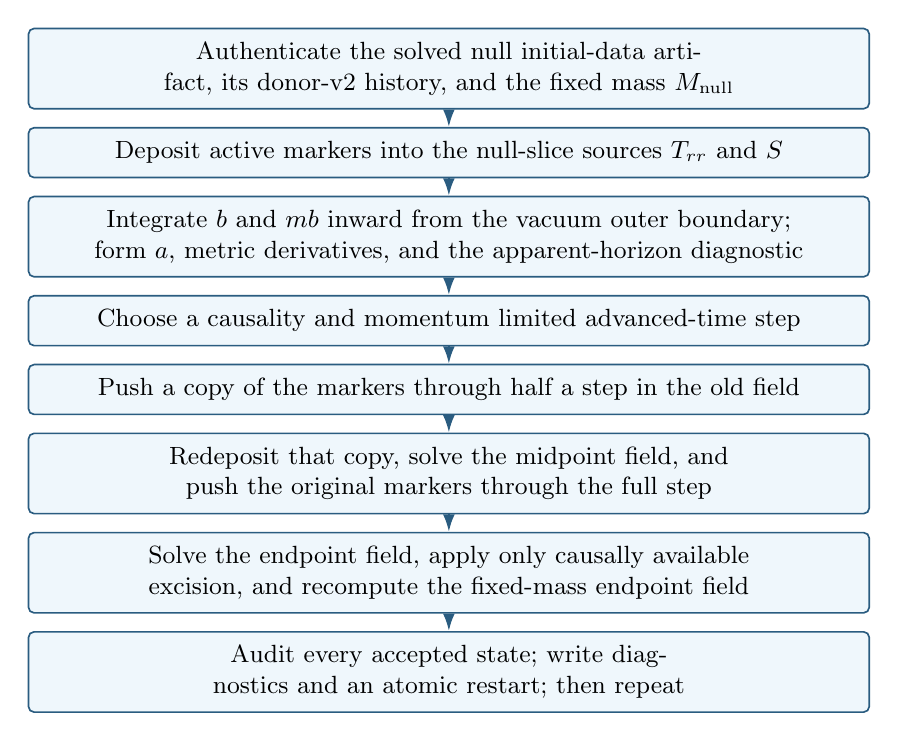
\begin{tikzpicture}[node distance=0.22cm]
\node[physicsflow] (ef1) {Authenticate the solved null initial-data artifact, its donor-v2 history, and the fixed mass \(M_{\rm null}\)};
\node[physicsflow,below=of ef1] (ef2) {Deposit active markers into the null-slice sources \(T_{rr}\) and \(S\)};
\node[physicsflow,below=of ef2] (ef3) {Integrate \(b\) and \(mb\) inward from the vacuum outer boundary; form \(a\), metric derivatives, and the apparent-horizon diagnostic};
\node[physicsflow,below=of ef3] (ef4) {Choose a causality and momentum limited advanced-time step};
\node[physicsflow,below=of ef4] (ef5) {Push a copy of the markers through half a step in the old field};
\node[physicsflow,below=of ef5] (ef6) {Redeposit that copy, solve the midpoint field, and push the original markers through the full step};
\node[physicsflow,below=of ef6] (ef7) {Solve the endpoint field, apply only causally available excision, and recompute the fixed-mass endpoint field};
\node[physicsflow,below=of ef7] (ef8) {Audit every accepted state; write diagnostics and an atomic restart; then repeat};
\draw[physicsarrow] (ef1) -- (ef2);
\draw[physicsarrow] (ef2) -- (ef3);
\draw[physicsarrow] (ef3) -- (ef4);
\draw[physicsarrow] (ef4) -- (ef5);
\draw[physicsarrow] (ef5) -- (ef6);
\draw[physicsarrow] (ef6) -- (ef7);
\draw[physicsarrow] (ef7) -- (ef8);
\end{tikzpicture}
\caption{Code-logic flow for one production ingoing-EF Einstein--Vlasov
WPIC update.  The fixed null-slice mass is retained when interior marker
sources are excised.}
\label{fig:ef-code-logic-flowchart}
\end{figure}

\paragraph{Initial data and first field solve.}
A fresh production EF run is allowed only in the high-compactness scenario,
on a linear radial grid with the configured origin-parity mesh convention.
It must receive both the authenticated coordinate-neutral physical initial
condition and a solved EF null artifact.  The artifact records the
worldline/null-surface intersections, EF marker momenta, reconstructed
center/face fields, map errors, donor ledger, hashes, and \(M_{\rm null}\).
Supplying only a spacelike SC marker file is a hard error.  The driver verifies
the physical-initial-condition hash, base and realized fingerprints, sampling
realization, marker count and grid, map-manifest hash, artifact hashes, and
initial metric/stress pullbacks before evolution.  Its first and all later
constraint solves use the inward boundary condition
\(Y(R_E)=M_{\rm null}\).  The regular-center mode (IEF35) remains available
only as a reusable library mode and unit-test target.

A restart is an atomic checkpoint containing the state needed to continue the
same evolution.  A resume reads the EF markers, advanced time, step number,
excision mode, and fixed boundary mass, then reconstructs the metric from
those markers. When physical or null initial data are supplied, it compares
each marker's invariant rest weight, angular momentum, identifier, and source
identifier with that authenticated realization before opening output files.
An accepted-step audit sidecar is trusted only when its exact
step number and advanced time match the restart.  A missing, stale, or
old-schema sidecar does not invent evidence: evolution may continue, but
black hole certification remains disabled until a complete new audit exists.
Here a sidecar is a separate atomic evidence file tied to the checkpoint; a
run summary is the machine-readable record of a completed run, and a
certificate is a separately authenticated record that promotes a scientific
claim only after all named checks pass.
Atomic means that the completed file replaces the old file as one operation,
so an interrupted write is not mistaken for a valid checkpoint.

\paragraph{Boundary, horizon, and excision conditions.}
The map worldtube \(R_B\) and the EF evolution boundary \(R_E\) are distinct.
The extraction requires \(R_B\le R_E\); the initial null surface between them
may use the audited analytic vacuum extension.  Evolution uses the full
domain through \(R_E\).  At the outer boundary,
\(b(R_E)=1\) and \(Y(R_E)=M_{\rm null}\).  This assumes the boundary stays in
vacuum; fixed total mass cannot reconstruct the finite-radius field of
dynamically important matter that has left the grid.
An escaped marker is an active marker that leaves the evolution domain; its
record and rest weight remain in accounting, but it no longer deposits on the
finite grid.

At the inner side, the origin-parity option creates a true \(r=0\) field face
but does not reflect EF characteristics.  Before an excision surface exists,
an active marker must remain at positive radius inside the field domain.
An attempted inner crossing rejects the trial step; the interior-evolution driver
retries with a smaller timestep as described below.
The characteristic equations are singular at \(r=0\) for \(\eta>0\).

The metric solver searches face intervals for the outermost
negative-to-positive zero of \(a\) and interpolates \(r^2a\) to obtain the
apparent-horizon radius \(r_H\), with \(m_H=r_H/2\).  Excision is enabled only
after a cell center satisfies \(a<a_{\rm ex}<0\); the particle boundary is
placed a configured number of cell centers farther inward and at most a fraction
\(F=0.1\) of the apparent-horizon radius.  The selected center, every center in the outward buffer, and the intervening
faces must satisfy \(a<a_{\rm ex}\), with finite positive \(b\).  A trapped outer
shell surrounding an untrapped central cavity therefore supplies a boundary
only when a qualifying trapped center lies within this radius cap.  Markers at or
inside it change from active to excised, keep their records and invariant
weights, stop depositing, and are no longer pushed.  The endpoint field is
then recomputed with fixed \(M_{\rm null}\).  No inner boundary data are
supplied inside this trapped, causally disconnected region.
An excision radius already present in the old field is enforced during every
frozen-metric push.  An endpoint-supported candidate boundary
is selected from the recomputed trapped region; it is applied before the step is
accepted and that endpoint field is recomputed. The retained boundary is
checked in this recomputed metric, including its buffer and radius cap.

The option \code{--ef-evolve-interior} retains all interior markers. Horizon
detection continues, while every metric stage sets the applied excision
radius to zero. The markers continue to move and deposit their stress.
Section~\ref{sec:ef-interior-evolution} gives the timestep, restart, and resolution
conditions for this mode.

\paragraph{Time integration, rejection, and accepted-state audit.}
The production driver uses two equal characteristic substeps and
\(C_{\rm CFL}=0.20\), where the Courant--Friedrichs--Lewy (CFL) number limits
radial travel and momentum change per step.  Internally the RK4 pusher evolves
\(u=\log P\), which preserves the mathematical \(P>0\) branch without imposing
a momentum floor.  A nonfinite characteristic stage, invalid logarithmic
state, or retryable right-hand-side (RHS) or RK4 failure rejects the whole
self-consistent step;
the driver halves \(\Delta v\) and retries, at most 24 times. In interior-evolution
mode, an attempted inner crossing or a nonfinite trial constraint solve also
allows this retry. The last accepted state is saved when the available
retries or floating-point time resolution are exhausted in interior-evolution mode.

Before output cadence is considered, every accepted state is audited for
finite markers, sources, center and face metric arrays, \(P>0\), \(b>0\),
fixed-\(M_{\rm null}\) agreement, causal excision, and positive excised weight
when excision is claimed.  Saved history then records marker-weight channels,
ADM mass, compactness, minimum \(a\) and \(b\), horizon and excision radii,
Lagrangian radii, virial and Jeans diagnostics.  Full stress profiles support
independent coordinate pullbacks.  General independent residuals of
(IEF28)--(IEF31) and a generic evolved-exterior vacuum norm are recommended
validation diagnostics, but are not currently emitted as ordinary
production-history columns; the implemented exact-vacuum residual belongs to
the authenticated null-map extension audit.
\subsubsection{Detailed coordinate map, donor-v2 history, and fail-closed provenance}
\label{sec:ef-detailed-map}

Section~\ref{sec:ef-eikonal-construction} established the geometry and the
forward dynamical map.  This section records the component identities and
numerical evidence used by the implementation.  It is deliberately placed
after the field and particle equations because the map initializes those
equations and identifies the physical events used to compare them.

At one mapped event the covariant and contravariant radial metric blocks are
\begin{align}
 g^{\rm EF}_{vv}&=-ab^2=-F^2e^{2\mu},&
 g^{\rm EF}_{vr}&=b=F e^{\lambda+\mu},&
 g^{\rm EF}_{rr}&=0,                                    \tag{IEF38d-1}\\
 g_{\rm EF}^{vv}&=0,&
 g_{\rm EF}^{vr}&=b^{-1}=A e^{-\lambda-\mu},&
 g_{\rm EF}^{rr}&=a=e^{-2\lambda}.                       \tag{IEF38d-2}
\end{align}
These are component transformations, not an identification of the raw arrays
\((\lambda,\mu)\) and \((a,b)\).  The retarded root reverses the mixed term
and has \(b_{\rm out}<0\); the EF evolution namespace implements only the
future advanced branch \(b>0\).

For a static exterior, both directions of the transformation are
\begin{align}
 \dd v&=\dd\tau+e^{\lambda-\mu}\dd r
       =\dd\tau+\frac{\dd r}{ab},
 &v(\tau,r)&=\tau+\int^r\frac{\dd r'}{a(r')b(r')},       \tag{IEF40a}\\
 \dd\tau&=\dd v-\frac{\dd r}{ab},
 &\tau(v,r)&=v-\int^r\frac{\dd r'}{a(r')b(r')}.          \tag{IEF40b}
\end{align}
The corresponding metric functions satisfy
\[
 e^{2\lambda}=\frac1a,\qquad e^{2\mu}=ab^2,\qquad
 \lambda=-\frac12\log a,\qquad
 \mu=\log b+\frac12\log a.                               \tag{IEF40c}
\]
For a dynamical inverse map, the integrating factor in (IEF40d) must satisfy
\[
 \partial_r F=-\partial_v\left(\frac{F}{ab}\right),       \tag{IEF40e}
\]
and substitution gives
\[
 \dd s^2=-\frac{ab^2}{F^2}\dd\tau^2
          +\frac1a\dd r^2+r^2\dd\Omega^2.                \tag{IEF40f}
\]
Setting \(F=1\) in a time-dependent field would impose the extra restriction
\(\partial_v[(ab)^{-1}]=0\); it is not a freely available gauge choice.
Neither \(F\) nor the event correspondence can be reconstructed from one
metric snapshot.

All SC-to-EF transformations and their inverse checks are restricted to the
connected overlap with \(a>0\).  As \(a\to0^+\), \(e^{2\lambda}=1/a\) and
\(1/(ab)\) diverge, so SC data and the public momentum-map helpers stop.
Finite positive \(b\) leaves the EF metric and EF characteristics regular;
the restriction belongs to the comparison chart, not the EF evolution.

\paragraph{Momentum components carried by the mapped artifact.}
If \(w\) is the existing VENUS orthonormal radial momentum and
\[
 \epsilon=\sqrt{1+w^2+\frac{2\eta}{r^2}},
\]
then the polar-coordinate covector components and inverse-coordinate
derivatives at the same event are
\[
 p_\tau=-e^\mu\epsilon,\qquad
 p_r^{({\rm pol})}=e^\lambda w,\qquad
 \left.\partial_v\tau\right|_r=F,\qquad
 \left.\partial_r\tau\right|_v=-\frac{F}{ab}
 =-e^{\lambda-\mu}.                                    \tag{IEF41a}
\]
A momentum is a one-form,
\[
 p=p_\tau\dd\tau+p_r^{({\rm pol})}\dd r
   =p_v\dd v+P\dd r.                                  \tag{IEF41b}
\]
Its components transform with derivatives of the old coordinates.  Using
(IEF40d), and equivalently \(ab=F e^{\mu-\lambda}\), gives
\[
 \boxed{
 P=p_r^{({\rm pol})}+p_\tau
       \left.\partial_r\tau\right|_v
  =e^\lambda(w+\epsilon)
  =\frac{w+\epsilon}{\sqrt a}},\qquad
 p_v=p_\tau\left.\partial_v\tau\right|_r
    =-F e^\mu\epsilon.
\]
The integrating factor cancels from \(P\).  Hence (IEF42) remains an exact
pointwise identity for a dynamical coordinate map when its SC and EF
arguments describe the same event.  The helper needs \(a\), but not \(F\);
it does not determine which events on two different slices correspond.
For strongly infalling data the subtraction-free evaluation is
\[
 P=\frac{1+2\eta/r^2}{\sqrt a\,(\epsilon-w)}.
\]
The inverse map, defined only for \(a>0\), is
\[
 x:=\sqrt a\,P,\qquad
 w=\frac12\left(x-\frac{\chi}{x}\right),\qquad
 \epsilon=\frac12\left(x+\frac{\chi}{x}\right).       \tag{IEF44}
\]
The same covector transformation gives
\[
 \frac b2\left(aP+\frac\chi P\right)
 =-p_v=F e^\mu\epsilon.                               \tag{IEF45}
\]
Thus the right-hand side is \(e^\mu\epsilon\) in the static normalization
\(F=1\).  The factor \(F\) is essential in a general dynamical
polar-to-advanced coordinate transformation; it is already encoded in the EF
metric function \(b=F e^{\lambda+\mu}\).

For reference, the retarded/outgoing coordinate and its future-directed
signed momentum are
\[
 u_{\rm ret}=\tau-\int^r e^{\lambda-\mu}\dd r',\qquad
 b_{\rm out}=-e^{\lambda+\mu},\qquad
 (p_r)_{\rm out}=e^\lambda(w-\epsilon)<0.              \tag{IEF45a}
\]
East's physical-data recipe first evolves an outward/dispersing solution and
then uses \(t\mapsto-t\) to obtain its incoming time reverse.  With
\(w_{\rm in}=-w_{\rm out}\), it acts as
\[
 b_{\rm in}=-b_{\rm out}>0,\qquad
 (p_r)_{\rm in}=-(p_r)_{\rm out}>0,\qquad
 r_{\rm in}=r_{\rm out},\qquad
 \eta_{\rm in}=\eta_{\rm out}.                        \tag{IEF45b}
\]
and therefore
\[
 -(p_r)_{\rm out}
 =e^\lambda(\epsilon-w_{\rm out})
 =e^\lambda(\epsilon+w_{\rm in})=(p_r)_{\rm in}.       \tag{IEF45c}
\]
Time reversal here means more than replacing the printed time coordinate by
its negative: every radial velocity or momentum is reversed as well, while
positions, angular momentum magnitudes, and invariant weights are retained.
Changing \(t\) without changing \(w\) would not construct the incoming
solution.
VENUS does not use that operation to relabel an outgoing production run as its
physical collapse.  Its physical neutral shell receives the controlled inward
kick (IEF-S26), so the physical Schwarzschild evolution is already ingoing and
is never time-reversed.  The null-slice extractor nevertheless needs the part
of that physical solution at negative Schwarzschild times because a single
ingoing null slice intersects different radii at different \(\tau\).  It
obtains that history without backward numerical integration by making an
\emph{independent} donor copy and using East's construction exactly once:
\[
 s=-\tau,\qquad w_{\rm reverse}(s=0)=-w_{\rm physical}(\tau=0).
                                                               \tag{IEF45c-1}
\]
The copy is evolved forward in \(s\).  At a marker--null-surface crossing the
physical momentum is restored as
\(w_{\rm physical}=-w_{\rm reverse}\), after which (IEF42) gives the
future-directed \(P>0\).  Thus ``using \(t\mapsto-t\)'' refers only to this
auxiliary donor/history construction.  The incoming Schwarzschild run is
unchanged, and the EF characteristic pusher never reverses its time or its
momentum.

The public conversion routines implement (IEF42)--(IEF44), including the
stable infalling branch:
\codesource{SC--EF marker-momentum conversion}{\path{cpu/include/ev/weighted_einstein_vlasov_pic_eddington_finkelstein.hpp}}{Public same-event momentum-map helpers and EF marker construction}
\begin{lstlisting}[language=C++,basicstyle=\ttfamily\scriptsize]
namespace ef = ev::eddington_finkelstein;

const double p_r = ef::canonical_p_r_from_schwarzschild_w(
    marker.w, marker.eta, marker.r, metric_gap);
ef::Marker ef_marker = ef::from_schwarzschild_marker(
    marker, metric_gap);

const double w = ef::schwarzschild_w_from_canonical_p_r(
    ef_marker.p_r, ef_marker.eta, ef_marker.r, metric_gap);

const double p_r_out =
    ef::outgoing_canonical_p_r_from_schwarzschild_w(
        outgoing_w, eta, radius, metric_gap);
const double p_r_in =
    ef::time_reverse_outgoing_canonical_p_r(p_r_out);
\end{lstlisting}
The marker rest weight and \(\eta\), its persistent identifier (ID), and its
source identifier are unchanged by this conversion.

The production extractor makes the separation between physical and reverse
states explicit (irrelevant checks are elided here):
\codesource{Solved-null initial-data extraction}{\path{cpu/src/drivers/einstein_vlasov_wpic.cpp}}{Production reverse-donor copy, eikonal solve, deterministic replay, and marker crossings}
\begin{lstlisting}[language=C++,basicstyle=\ttfamily\scriptsize]
std::vector<ev::WeightedPICMarker> reverse_initial = physical_markers;
for (auto& marker : reverse_initial) {
    marker.w = -marker.w;                 // s=-tau donor only
}
std::vector<ev::WeightedPICMarker> donor_markers = reverse_initial;
// Store every accepted donor field and the exact accepted-dt ledger.
map::EikonalSurface surface = map::solve_ingress_eikonal_surface(
    history, grid, reverse_time, 8);
// Replay the ledger bit-for-bit and require one crossing for every ID.
crossings.push_back(map::interpolate_marker_crossing(
    before[q], replay[q], replay_time, next_time,
    surface, history, grid, step + 1));
\end{lstlisting}
The integer passed to the surface solver is \(n\), the number of RK4
substeps used for the coarse solve on each radial cell.  Starting from the
same already accepted state \(Y_{i,\mathrm{in}}\) at the outer end of cell
\(i\), the extractor independently computes an \(n\)-substep result
\(Y_i^{(n)}\) and a \(2n\)-substep result \(Y_i^{(2n)}\), where

\[
        Y=(s_\sigma,\log A).
\]
It accepts \(Y_i^{(2n)}\) as the incoming state for the next cell; it does not
advance with the coarse result and does not Richardson-extrapolate the state.
For each component it estimates the local error of that accepted, refined
fourth-order result by
\begin{align}
 \epsilon_{s,i}
 &=\frac{\left|s_{\sigma,i}^{(2n)}-s_{\sigma,i}^{(n)}\right|}
 {\left(2^4-1\right)
  \max\!\left(1,
       \left|s_{\sigma,i,\mathrm{in}}\right|,
       \left|s_{\sigma,i}^{(2n)}\right|\right)},                 \tag{IEF45c-2}\\
 \epsilon_{\log A,i}
 &=\frac{\left|\left(\log A\right)_i^{(2n)}
                    -\left(\log A\right)_i^{(n)}\right|}
 {\left(2^4-1\right)
  \max\!\left(1,
       \left|\left(\log A\right)_{i,\mathrm{in}}\right|,
       \left|\left(\log A\right)_i^{(2n)}\right|\right)} .       \tag{IEF45c-3}
\end{align}
The unit term gives a dimensionless error that behaves as an absolute error
for small values and a relative error for large ones.  It uses one code-time
unit for \(s_\sigma\).  The factor \(2^4-1=15\) is the RK4
step-doubling Richardson divisor.  The surface records the two maxima
separately as
\texttt{maximum\_reverse\_time\_richardson\_error} and
\texttt{maximum\_log\_A\_richardson\_error}.  The authenticated manifest
serializes them unambiguously as
\path{maximum_eikonal_reverse_time_richardson_error} and
\path{maximum_eikonal_log_A_richardson_error}, together with the exact
normalization string in (IEF45c-2)--(IEF45c-3).  Its backward-compatible
aggregate is exactly
\[
 \texttt{maximum\_eikonal\_ode\_residual}
 =\max_i\left\{\epsilon_{s,i},\epsilon_{\log A,i}\right\}.       \tag{IEF45c-4}
\]
Despite its retained manifest name, (IEF45c-4) is an integration-error
estimate, not the finite-difference quantity

\[
 \left|\frac{\Delta s_\sigma}{\Delta r}
              -h(s_{\mathrm{mid}},r_{\mathrm{mid}})\right| .     \tag{IEF45c-5}
\]
The latter includes the midpoint quadrature defect produced by the curvature
of the physical null ray.  It can therefore remain larger than the RK4
integration error even when the ray is accurately integrated.  It is not used as an acceptance residual.
The null-map preflight applies the same, unchanged \(2\times10^{-5}\)
ceiling to each authenticated extraction component and to their aggregate.
This integration-error estimate separates RK4 error from the physical
curvature of the ray while preserving the acceptance tolerance.  The later same-event history comparator solves a
different initial-value problem for each sampled event.  It deliberately
uses the still more conservative raw \(n\)-versus-\(2n\) change described
below, rather than assuming that a ray crossing time-interpolation knots is
already in the smooth fourth-order Richardson regime.

The binary null slice and its manifest, crossing table, mapped field slice,
accepted-step ledger, and dense donor history are all recorded with the
256-bit Secure Hash Algorithm (SHA-256).  A
fresh EF run refuses to start without this solved-eikonal artifact and verifies
the base initial condition (IC), realized Schwarzschild IC, sampling
realization, grid, angular
controls, marker identities, and all nested artifact hashes.

\paragraph{Separated map worldtube and evolution boundary.}
The outer radius is part of the characteristic initial-data problem, not a
harmless output choice.  VENUS therefore distinguishes the exact mesh-face
worldtube \(R_B\), set by \code{--ef-map-worldtube-radius}, where the numerical
eikonal solve is normalized, from the full EF evolution boundary \(R_E\), set
by \code{--high-r-max}.  They obey
\[
 0<R_B\leq R_E,\qquad R_B>2M_{\rm null}.                \tag{IEF45c-6}
\]
The legacy case is \(R_B=R_E\).  When \(R_B<R_E\), every matter worldline has
already crossed the selected null surface strictly inside \(R_B\), so the
remainder of that \emph{initial null slice} is known analytically.  Define
\[
 \Delta r_\star(r;R_B,M)=
 \begin{cases}
 r-R_B, &M=0,\\[2pt]
 (r-R_B)+2M\log\!\left(\dfrac{r-2M}{R_B-2M}\right),&M>0,
 \end{cases}                                           \tag{IEF45c-7a}
\]
which is \(r_\star(r)-r_\star(R_B)\) without a logarithm of a dimensionful
quantity.  If \(s=-\tau\), and \(s_B\) is the reverse-donor time at the
worldtube, the exact extension for \(R_B<r\leq R_E\) is
\begin{align}
 s(r)&=s_B+\Delta r_\star(r;R_B,M_{\rm null}),&
 \tau(r)&=-s_B-\Delta r_\star(r;R_B,M_{\rm null}),
                                                               \tag{IEF45c-7b}\\
 m(r)&=M_{\rm null},&
 a(r)&=1-\frac{2M_{\rm null}}r,                       \tag{IEF45c-7c}\\
 A(r)&=F(r)=b(r)=1,&
 T_{ab}(r)&=S(r)=0.                                    \tag{IEF45c-7d}
\end{align}
In particular, \(F=1\), not \(1/a\).  The radial derivative of the inverse
time map at fixed \(v\) is instead
\[
 \left.\frac{\partial\tau}{\partial r}\right|_v
 =-\frac{F}{ab}=-\frac1a,                              \tag{IEF45c-7e}
\]
exactly as the vacuum tortoise relation requires.  The mass in this extension
is \(M_{\rm null}\), the ADM mass on the extracted null slice; using
\(M_{\rm family}\) or the independently deposited \(M_{\rm dep}\) would
introduce a boundary inconsistency.

The eikonal construction labels the extracted surface by \(v=-T_{\rm donor}\)
at the normalized worldtube.  Runtime output shifts only the additive time
origin:
\[
 \boxed{\ \widehat v:=v+T_{\rm donor}\ },
 \qquad \widehat v=0\quad\hbox{on the imported initial null slice}.          \tag{IEF45c-7f}
\]
The manifest names the same quantity
\(\code{v_bar=v+ef_v_offset}\), with
\(\code{ef_v_offset}=T_{\rm donor}\).  No metric or momentum component is
changed by this constant relabelling.

This split is accepted only after all of the following fail-closed gates:
\begin{enumerate}
\item \(R_B\) is an exact non-inner edge of the full \(R_E\) mesh, so the
      numerically mapped cells form one authenticated grid prefix;
\item the last four donor cells below \(R_B\) have vanishing matter sources,
      the discrete vacuum value \(e^{\lambda+\mu}=1\) satisfies its recorded
      \(O(\Delta r_B^2)\) tolerance, and every donor worldline remains at
      least four local cells inside \(R_B\);
\item every persistent marker ID has one and only one surface crossing, each
      crossing has four-cell clearance from \(R_B\), and no marker reaches
      the finite evolution boundary first;
\item the complete numerical surface lies inside the dense donor history,
      \(A>0\), \(F>0\), \(a>0\) throughout the overlap, and the two separate
      RK4 step-doubling errors in (IEF45c-2)--(IEF45c-4) pass;
\item the analytic part has zero source, constant \(m=M_{\rm null}\),
      \(A=F=b=1\), positive \(a\), and vanishing field and inverse-map
      residuals at their recorded tolerance.
\end{enumerate}
The version-2 binary and JavaScript Object Notation (JSON) manifest record
\(R_B\), \(R_E\), the analytic
extension start index, separate prefix and full-grid fingerprints, both
clearances, vacuum-source and \(b\)-normalization audits, and all analytic
extension residuals.  These metadata and the slice, crossing table,
accepted-step ledger, donor history, physical IC, and nested hashes are
authenticated again on EF import and resume.

The analytic continuation in (IEF45c-7a)--(IEF45c-7e) constructs only the
vacuum part of the \emph{initial} characteristic surface.  It does not freeze
the region \(R_B<r<R_E\) during evolution: after import the EF constraints and
characteristics are evolved on the complete \(R_E\) grid.  Nor do values of
\(R_B,R_E,T_{\rm donor}\), marker count, or grid resolution transfer from an
older Gaussian-shell experiment.  The bound static-shell family below must
derive all of them from its own local crossing/vacuum preflight before any
long job is submitted.

\paragraph{Slice caveat.}
Equations (IEF39)--(IEF44) are an algebraic/radial map only for a static
solution.  Dynamically, (IEF38a)--(IEF40e) must first determine which events
correspond.  The pointwise momentum identity (IEF42) remains exact at those
events, but the pointwise conversion helpers in the EF kernel neither solve
the eikonal PDE nor resample a hypersurface; the separate authenticated
coordinate-map pipeline described below performs those operations.  A
\(\tau={\rm const}\) surface is spacelike whereas a
\(v={\rm const}\) surface is null, and \(v=0\) generally samples different SC
times at different radii.  A rigorous cross-coordinate validation should
therefore use a transformed static state, an analytic worldline, or
the same physical events in a dynamical spacetime.  Merely copying the same radial arrays
into both modules does not create identical physical initial hypersurfaces.

\paragraph{What equality of the two coordinate descriptions means.}
This point is essential for interpreting any SC--EF comparison.  The
distribution function is a scalar on the future mass shell, not an array
whose entries may be compared at the same pair of numerical time and radial
indices.  At one and the same event, with the momenta related by
(IEF42)--(IEF44), scalar invariance is the statement
\[
 f_{\rm EF}\bigl(v(\tau,r),r,P,\eta\bigr)
 =f_{\rm SC}\bigl(\tau,r,w,\eta\bigr).             \tag{IEF45d}
\]
There is no multiplicative Jacobian in (IEF45d).  A histogram density per
coordinate momentum interval does carry one: if
\(n_w\,\dd w=n_P\,\dd P\), then
\[
 n_P=n_w\left|\frac{\partial w}{\partial P}\right|,
 \qquad
 \frac{\partial w}{\partial P}
 =\frac{\sqrt a}{2}\left(1+\frac{\chi}{aP^2}\right). \tag{IEF45e}
\]
WPIC marker rest weights are invariant particle-number weights and therefore
remain unchanged; (IEF45e) is relevant only when the empirical measure is
converted into a density in a chosen momentum coordinate.
The forward Jacobian and the reduced invariant mass-shell measure make this
distinction explicit:
\[
 \frac{\partial P}{\partial w}=\frac P\epsilon>0,
 \qquad
 \boxed{\;\frac{\dd P}{P}=\frac{\dd w}{\epsilon}\;},
 \qquad
 \dd\Pi_{\rm red}
 =\frac{2\pi}{r^2}\frac{\dd w\,\dd\eta}{\epsilon}
 =\frac{2\pi}{r^2}\frac{\dd P\,\dd\eta}{P}.      \tag{IEF45e-1}
\]
Thus substituting the scalar relation (IEF45d) and (IEF45e-1) into the
stress integrals reproduces the same tensor without an ad hoc rescaling of
\(f\).

A finite WPIC realization does not provide a pointwise value of the smooth
continuum function \(f\).  It represents an empirical mass-shell measure,
defined transparently by its action on any smooth test function \(\psi\).
Let \(\Sigma\) be the physical hypersurface being sampled, let the same symbol
also denote the set of marker worldlines intersecting it, and let \(W_p\) be
the invariant rest-number weight of marker \(p\).  Then
\[
 \widehat f_{\Sigma}[\psi]
 :=\sum_{p\in\Sigma}W_p\,
   \psi(r_p,\pi_p,\eta_p),                              \tag{IEF45e-1a}
\]
where \(\pi_p\) denotes the chosen radial momentum coordinate:
\(\pi_p=w_p\) on an SC slice and \(\pi_p=P_p\) on an EF slice.  Equality
of the sampled distribution means equality of this measure after each marker
worldline is intersected with the same physical hypersurface and its momentum
is transformed with (IEF42)--(IEF44).  The strict certificate therefore
authenticates unique persistent identifiers (IDs) and source IDs, invariant
\(W_p\) and
\(\eta_p\), mapped event positions, and transformed momenta.  Equality of all
of those atoms is equality of (IEF45e-1a) for every test function; the code
does not pretend to reconstruct arbitrary pointwise probes from a finite
marker set.  When a crossing or trajectory table supplies both
\code{f_schwarzschild} and \code{f_eddington_finkelstein}, their scalar
values are compared too, but explicit scalar-\(f\) columns are optional.
Thus two noisy coordinate histograms are never treated as pointwise samples
of \(f\).  A separately chosen smooth reconstruction may be compared using
(IEF45d)--(IEF45e), but that is an additional diagnostic, not a replacement
for empirical-measure identity.  Stress-tensor parity is checked independently
from the deposited moments below; agreement of finitely many moments alone
would not prove equality of the distribution.

There is also a spatial Jacobian because the two distributions live on
different hypersurfaces.  The reduced canonical phase measures are
\[
 \dd\Gamma_\tau=8\pi^2e^\lambda\,
       \dd r\,\dd w\,\dd\eta,
 \qquad
 \dd\Gamma_v=8\pi^2\,
       \dd r\,\dd P\,\dd\eta .                       \tag{IEF45e-2}
\]
Hamiltonian Liouville flow maps the first measure to the second when one
follows each worldline from its \(\tau\)-slice intersection to its
\(v\)-slice intersection.  The change in the intersection radius supplies
the spatial factor that complements \(\partial P/\partial w\).  This is why
a marker's represented particle number is copied unchanged; multiplying its
weight by either momentum Jacobian would count that factor twice.

The same distinction applies to moments.  Raw coordinate components of a
tensor are not expected to have the same numbers.  In SC variables the radial
stress-energy block reconstructed from the physical moments in (EWP10) is
\[
 T^{\rm SC}_{\tau\tau}=e^{2\mu}\rho,\qquad
 T^{\rm SC}_{\tau r}=-e^{\mu+\lambda}j,\qquad
 T^{\rm SC}_{rr}=e^{2\lambda}p_{\rm rad}.             \tag{IEF45f}
\]
The sign in the middle identity agrees with
\(\lambda_\tau=-4\pi r e^{\lambda+\mu}j\).
Let \(\zeta:=A h=v_r=(ab)^{-1}\), where \(\zeta\) is the forward null
slope and the last equality follows from
(IEF38d).  Pulling the EF tensor back with
\(v_\tau=A\), \(v_r=\zeta\), and \(r_\tau=0\) gives
\begin{align}
 T^{\rm SC}_{\tau\tau}
 &=A^2T^{\rm EF}_{vv},                                      \tag{IEF45g}\\
 T^{\rm SC}_{\tau r}
 &=A\bigl(\zeta T^{\rm EF}_{vv}+T^{\rm EF}_{vr}\bigr),   \tag{IEF45h}\\
 T^{\rm SC}_{rr}
 &=\zeta^2T^{\rm EF}_{vv}+2\zeta T^{\rm EF}_{vr}
   +T^{\rm EF}_{rr}.                                      \tag{IEF45i}
\end{align}
The angular components are unchanged because the angular coordinates are
unchanged.  Equivalently, the inverse formulas follow from
\(\tau_v=F\), \(\tau_r=-F/(ab)=-h\).  These identities require all of
\(T_{vv},T_{vr},T_{rr}\), not just the two source combinations used by the
EF radial constraints.  Equations (IEF18)--(IEF20) specify how the diagnostic
deposition must construct them.
Writing the inverse formulas in terms of the polar physical moments exposes
every sign and is useful for a direct code test.  The second line below
repeats the source identity (IEF45i-2):
\begin{align}
 T^{\rm EF}_{vv}&=F^2e^{2\mu}\rho,&
 T^{\rm EF}_{vr}&=-F e^{\lambda+\mu}(\rho+j)
                 =-b(\rho+j),                        \tag{IEF45i-1}\\
 T^{\rm EF}_{rr}&=e^{2\lambda}(\rho+2j+p_{\rm rad}),&
 S&=-\frac2bT^{\rm EF}_{vr}-aT^{\rm EF}_{rr}
   =\rho-p_{\rm rad}.                                    \notag
\end{align}
For one-direction tangential pressure
\[
 p_\perp=\frac{2\pi}{r^4}\int_0^\infty\!\!\int_0^\infty
       \frac{\eta}{\epsilon}f\,
       \dd\eta\,\dd w,
 \qquad T_{\theta\theta}=r^2p_\perp,\qquad
 T_{\phi\phi}=\sin^2\theta\,T_{\theta\theta}.       \tag{IEF45i-3}
\]
Equations (IEF45e-1) and (IEF42) turn (IEF18)--(IEF23) into
(IEF45i-1)--(IEF45i-3) term by term.

The coordinate Jacobian must likewise be applied to the metric.  The pullback
of (IEF2) to \((\tau,r)\) is
\begin{align}
 (g_{\tau\tau})_{\rm pullback}&=-ab^2A^2,                 \tag{IEF45j}\\
 (g_{\tau r})_{\rm pullback}&=-ab^2A\zeta+bA,            \tag{IEF45k}\\
 (g_{rr})_{\rm pullback}&=-ab^2\zeta^2+2b\zeta.          \tag{IEF45l}
\end{align}
For an exact map these are respectively
\(-e^{2\mu},0,e^{2\lambda}\).  Thus ``the metric is the same'' means that
(IEF45j)--(IEF45l), evaluated at mapped events, agree with the SC tensor; it
does not mean that the raw arrays \((a,b)\) equal \((\lambda,\mu)\).
The areal radius, Misner--Sharp mass
\(m=r(1-g^{ab}\partial_a r\partial_b r)/2=r(1-a)/2\), and scalar contractions
of \(T_{ab}\) provide additional coordinate-independent comparisons.

\paragraph{Solving the dynamical map numerically.}
For a complete SC spacetime history, define
\(h(\tau,r)=e^{\lambda-\mu}\), impose
\(v(\tau,R_B)=\tau\) on the common outer vacuum worldtube, and solve
the advanced eikonal equation (IEF38a), equivalently
\[
 \boxed{\ v_r-hv_\tau=0,\qquad v_\tau>0\ },            \tag{IEF45m}
\]
with the plus/ingoing root.  For one ingoing null slice labelled by its
boundary value \(v_{\cal B}\), its SC time \(\tau_{v_{\cal B}}(r)\) and the
inverse Jacobian factor \(F=\partial\tau/\partial v\) may be obtained without
finite-differencing two nearly equal null labels:
\begin{align}
 \frac{\dd\tau_{v_{\cal B}}}{\dd r}
 &=-h\bigl(\tau_{v_{\cal B}}(r),r\bigr),
 &\tau_{v_{\cal B}}(R_B)&=v_{\cal B},                  \tag{IEF45n}\\
 \frac{\dd F}{\dd r}
 &=-\partial_\tau h\bigl(\tau_{v_{\cal B}}(r),r\bigr)F,
 &F(R_B)&=1.                                             \tag{IEF45o}
\end{align}
Then \(A=F^{-1}\) and \(b=F e^{\lambda+\mu}\) on that slice.  Equations
(IEF45n)--(IEF45o) are the characteristic form of (IEF38c), not an additional
assumption.

Conversely, an EF history determines the SC label from the inverse eikonal
equation
\[
 \boxed{\ \tau_r+\frac{1}{ab}\tau_v=0,\qquad \tau_v>0\ },
 \qquad \tau(v,R_B)=v .                                 \tag{IEF45p}
\]
Along a surface of constant boundary SC label \(\tau_{\cal B}\), its EF
advanced time satisfies
\[
 \frac{\dd v_{\tau_{\cal B}}}{\dd r}
 =\frac{1}{a(v_{\tau_{\cal B}}(r),r)
             b(v_{\tau_{\cal B}}(r),r)},
 \qquad v_{\tau_{\cal B}}(R_B)=\tau_{\cal B}.         \tag{IEF45q}
\]
The same-event comparator also carries the coordinate Jacobians.  Directly
advancing a Jacobian sensitivity can give a negative number when an explicit
RK stage is stiff, although the exact, future-oriented map cannot change its
sign.  The comparator therefore advances logarithmic sensitivities.  Its
forward trace starts at the sampled SC event \((\tau_*,r_*)\), not at the
outer boundary:
\begin{align}
 \frac{\dd\tau_{\rm tr}}{\dd r}&=-h(\tau_{\rm tr},r),&
 \tau_{\rm tr}(r_*)&=\tau_*,\notag\\
 \frac{\dd\ell_A}{\dd r}&=-\partial_\tau h(\tau_{\rm tr},r),&
 \ell_A(r_*)&=0,\qquad
 A(\tau_*,r_*)=e^{\ell_A(R_B)}>0 .          \tag{IEF45q-1}
\end{align}
Here the subscript ``tr'' means the value being carried along the trace.
Because \(v=\tau\) at \(R_B\), the endpoint
\(\tau_{\rm tr}(R_B)\) is the advanced-time label \(v(\tau_*,r_*)\), up to
the recorded constant time-origin offset.  The tangent equation for
\(\ell_A\) is just the derivative of the ray endpoint with respect to its
starting time.  The inverse trace starts instead at the sampled EF event
\((v_*,r_*)\):
\begin{align}
 \frac{\dd v_{\rm tr}}{\dd r}&=\zeta_{\rm inv}(v_{\rm tr},r),&
 v_{\rm tr}(r_*)&=v_*,\notag\\
 \frac{\dd\ell_F}{\dd r}&=\partial_v\zeta_{\rm inv}(v_{\rm tr},r),&
 \ell_F(r_*)&=0,\qquad
 F(v_*,r_*)=e^{\ell_F(R_B)}>0,               \tag{IEF45q-2}\\
 h&=e^{\lambda-\mu},&\zeta_{\rm inv}&:=(ab)^{-1}.      \tag{IEF45q-3}
\end{align}
At the inverse endpoint, \(v_{\rm tr}(R_B)\) gives the reconstructed SC time
\(\tau(v_*,r_*)\), again after applying the recorded time-origin offset.
Define the two terminal log Jacobians
\(q_A:=\ell_A(R_B)=\log A(\tau_*,r_*)\) and
\(q_F:=\ell_F(R_B)=\log F(v_*,r_*)\).  These are the values serialized by the
comparator.  Advancing \(\ell_A\) and \(\ell_F\) is an exact change of
variables, not an approximation or a sign repair.  A finite terminal value
always gives a positive Jacobian; a value outside floating-point range makes
the audit inconclusive and is never clipped.

The signs look opposite if one writes differential equations for the
Jacobian \emph{fields} with the outer-boundary value fixed, because the code
instead propagates an identity sensitivity from the event outward.  Along
the corresponding constant-label rays, the field equations are
\[
 \boxed{\quad
 \left.\frac{\dd\ln A}{\dd r}\right|_{v}
     =+\partial_\tau e^{\lambda-\mu},
 \qquad
 \left.\frac{\dd\ln F}{\dd r}\right|_{\tau}
     =-\partial_v\!\left(\frac1{ab}\right)
 \quad} .                                             \tag{IEF45q-3a}
\]
Thus (IEF45q-1)--(IEF45q-2) and (IEF45q-3a) describe the same derivatives
with opposite integration orientations.  Each code trace initializes its
sensitivity to one at \(r_*\), so its logarithm starts at zero.

The comparator reconstructs the \emph{same spatial metric interpolant} used
by the particle and null-map pushers.  Its comparison must therefore include
both cell-center and face data, since together they determine the metric
between stored points.  In one half-cell let \(x_0<x_1\)
be the face and center radii (or the center and face radii), set
\(\xi=(r-x_0)/(x_1-x_0)\), and attach subscripts \(0,1\) to the corresponding
endpoint data.  The production SC sampler uses
\begin{align}
 \lambda(r)&=(1-\xi)\lambda_0+\xi\lambda_1,             \tag{IEF45q-3b}\\
 \mu(r)&=(2\xi^3-3\xi^2+1)\mu_0
 +(\xi^3-2\xi^2+\xi)\Delta r\,d_0 \notag\\
 &\quad+(-2\xi^3+3\xi^2)\mu_1
 +(\xi^3-\xi^2)\Delta r\,d_1,                         \tag{IEF45q-3c}
\end{align}
where \(\Delta r=x_1-x_0\) and \(d_0,d_1\) are the saved radial derivatives
of \(\mu\).  Equation (IEF45q-3c) is an ordinary cubic joining the saved
endpoint values and slopes.  Its slope limiter is also reproduced exactly:
with secant \(\delta=(\mu_1-\mu_0)/\Delta r\), both slopes are set to zero if
\(\delta\leq0\).  Otherwise negative slopes are replaced by zero; writing
\(\alpha=d_0/\delta\) and \(\beta=d_1/\delta\), both remaining slopes are
multiplied by \(3/\sqrt{\alpha^2+\beta^2}\) when
\(\alpha^2+\beta^2>9\).  This prevents an interpolated lapse overshoot
between two valid stored points.

The code then forms
\(h=\exp[\lambda(r)-\mu(r)]\) separately on the two saved time slices and
linearly interpolates those two values in time.  The order matters:
exponentiating node values first, or linearly joining center values across a
whole cell, defines a different discrete spacetime.  On the EF side, the
production sampler linearly joins face and center values of \(a\) and \(b\)
on each half-cell; the comparator does the same before interpolating those
values in \(v\) and differentiating the resulting piecewise-linear time
history in (IEF45q-2).

The SC profile therefore saves the left/right face radii, face values of
\(\lambda,\mu,\mu_r\), and the center value of \(\mu_r\) beside every center
row.  The EF profile saves the same face locations and the left/right face
values of \(a,b\).  The authenticated \code{VENUSSCHIST1} version-2 donor
history saves the full SC face reconstruction for every negative-\(\tau\)
snapshot as well.  This last point is essential because an early same-event
ray can enter the time-reversed donor segment.  A legacy center-only profile
or version-1 donor may still be inspected diagnostically, but it is marked as
using a different center-to-center interpolant and cannot issue a production
parity certificate.  This fail-closed rule prevents a substep-independent
interpolation floor from being mistaken for a failure of RK4 convergence.

Let subscripts \(n\) and \(2n\) denote otherwise identical per-cell RK4
traces.  The history-comparison gate uses
\begin{align}
 E_{\rm fwd}
 &=\max\!\left(
      |v_{2n}-v_n|,
      |q_{A,2n}-q_{A,n}|
    \right),                                           \tag{IEF45q-4}\\
 E_{\rm inv}
 &=\max\!\left(
      |\tau_{2n}-\tau_n|,
      |q_{F,2n}-q_{F,n}|
    \right).                                           \tag{IEF45q-5}
\end{align}
Both must be at most \(2\times10^{-5}\).  No factor of \(15\) and no division
by \(|q_A|\) or \(|q_F|\) is used here.  The absolute change in \(\log A\)
directly measures the multiplicative change in \(A\); dividing it by a large
\(|\log A|\) could hide a percent-level Jacobian error.  A Richardson factor
would additionally presume a demonstrated smooth fourth-order regime, which
piecewise-linear saved histories need not have when a ray crosses a time
knot.  Increasing the substeps must make (IEF45q-4)--(IEF45q-5) converge at
the unchanged ceiling before a coordinate certificate can pass.

The implementation follows the displayed definition literally:
\codesource{Dynamic SC--EF coordinate comparator}{\path{cpu/tools/compare_wpic_dynamic_coordinates.py}}{Forward and inverse eikonal step-refinement gate}
\begin{lstlisting}[language=Python,basicstyle=\ttfamily\scriptsize]
time_change = abs(time_2n - time_n)
log_jacobian_change = abs(log_jacobian_2n - log_jacobian_n)
step_refinement_error = max(time_change, log_jacobian_change)
if step_refinement_error > eikonal_convergence_tolerance:
    status = "forward_eikonal_not_converged"  # or inverse
\end{lstlisting}
The output records the two component changes, their maximum, the substep
count, and the event with the largest error.  These values reproduce the
acceptance decision directly from the saved comparison.

For a production parity campaign, the integer \(n\) is not an implicit code
default.  The submission helper requires one explicitly chosen positive value
through \code{VENUS_EIKONAL_SUBSTEPS}.  That same value is passed to all four
resolution--realization diagnostics, written into the convergence evidence,
and required again by the terminal certificate.  Each diagnostic evaluates
both \(n\) and \(2n\), tests their raw difference in
(IEF45q-4)--(IEF45q-5), and keeps the more refined \(2n\) solution for the
same-event comparison.  A missing, zero, or inconsistent value stops the
chain; it is never replaced silently by a local default.

The calculation records the source identities for its numerical evidence.  Its Slurm
scripts and scientific Python tools are fixed under the staged
\code{VENUS_SOURCE_ROOT}.  Their SHA-256 identities are measured at
submission, checked before and after each dependent job, and carried into the
convergence record and final certificate.  Environment variables cannot
replace these production tools or Slurm scripts.  The hash checks bind each result to the comparator and convergence code
that produced it.

The two independently reconstructed maps must close:
\(\tau_{\rm EF}(v_{\rm SC}(\tau,r),r)=\tau\).  Required numerical residuals
are
\begin{align}
 R_v&=-e^{-2\mu}v_\tau^2+e^{-2\lambda}v_r^2,           \tag{IEF45r}\\
 R_\tau&=\tau_r+(ab)^{-1}\tau_v,                       \tag{IEF45s}\\
 R_{\rm inv}&=\tau_{\rm EF}(v_{\rm SC}(\tau,r),r)-\tau.\tag{IEF45t}
\end{align}
They must be reported, rather than assuming the static tortoise formula in a
time-dependent region.
The Jacobian part of the closure test is evaluated without subtracting two
large products,
\[
R_{AF}=\left|\operatorname{expm1}(q_A+q_F)\right|
       =|AF-1|,                                        \tag{IEF45t-1}
\]
Here \(\operatorname{expm1}(x)\) is the floating-point operation that
evaluates \(e^x-1\) accurately when \(x\) is small.
Any exponential overflow fails closed.  The comparator's dimensionless
time-closure gate is exactly
\[
 E_{\rm comp}^{\tau}
 =\frac{|\tau_{\rm EF}(v_{\rm SC}(\tau,r),r)-\tau|}
        {\max(1,|\tau|,|\tau_{\rm EF}|)},
 \qquad
 \max(E_{\rm comp}^{\tau},R_{AF})\le5\times10^{-4}    \tag{IEF45t-2}
\]
by default.  Thus the raw eikonal step-refinement test
(IEF45q-4)--(IEF45q-5) and the normalized map-composition test are distinct
quantities and are reported separately.

\paragraph{Dynamical initial data on an ingoing null surface.}
The coordinate-neutral marker file currently used by the driver fixes the
same random realization, weights, \(r,w,\eta\), and IDs.  That is valuable
for controlling particle-in-cell (PIC) noise, but by itself it is
\emph{not} a transformed
dynamical initial data set: inserting it on both \(\tau=0\) and \(v=0\)
places the markers at different spacetime events.  A production comparison of the same physical evolution requires
characteristic extraction:
\begin{enumerate}
\item Evolve and densely checkpoint the SC metric and every marker worldline
      over the time interval crossed by a chosen ingoing null surface.
\item Solve (IEF45n)--(IEF45o) from the outer vacuum worldtube.  For every
      marker ID, find the unique intersection of its timelike worldline with
      \(\tau=\tau_{v_{\cal B}}(r)\).  A bracketed scalar root may be used:
      \(G_p(\tau)=v(\tau,r_p(\tau))-v_{\cal B}\).  Since the SC
      characteristic has
      \(\dd r_p/\dd\tau=e^{\mu-\lambda}w_p/\epsilon_p\),
      \[
       \frac{\dd G_p}{\dd\tau}
       =A\left(1+\frac{w_p}{\epsilon_p}\right)>0,     \tag{IEF45u}
      \]
      where \(\epsilon_p>|w_p|\) for a massive marker.  Hence a crossing,
      once bracketed, is unique and future oriented.
\item At each intersection retain its invariant rest weight, \(\eta\), and
      IDs, and transform its covector using (IEF42).  Interpolate the SC metric
      to the same null surface and construct \(a=e^{-2\lambda}\) and
      \(b=F e^{\lambda+\mu}\).
\item Deposit the extracted marker ensemble and require the EF constraint
      solution to converge to those transformed metric and stress-tensor
      data.  Only this extracted artifact is a valid EF initial state for the
      dynamical parity run.
\item In the common future, solve (IEF45m) and (IEF45p), intersect paired
      marker worldlines with common physical slices, and compare marker
      \((r,w,\eta)\), the scalar distribution via (IEF45d), all moments via
      (IEF45f)--(IEF45i), and the metric via (IEF45j)--(IEF45l).
\end{enumerate}
The SC history must extend far enough that the entire null slice, including
its innermost point, lies in the stored domain.  A surface truncated before
all marker intersections is not valid characteristic data.

\paragraph{Well-posedness and discretization domain.}
On a smooth polar exterior, \(c=e^{\mu-\lambda}\) is positive and locally
Lipschitz.  The ray equation in (IEF38c-1) then has unique solutions, so two
radial ingoing characteristics cannot cross at \(r>0\).  The spherical
congruence does focus at \(r=0\), which is its ordinary central caustic and
the endpoint of this one-sided areal-radius map.  The other endpoint is a
polar-coordinate horizon: the construction requires
\[
 a=e^{-2\lambda}>0,\qquad A=v_\tau>0,\qquad
 \det\frac{\partial(v,r)}{\partial(\tau,r)}=A,        \tag{IEF45v}
\]
and becomes singular in the polar variables as \(a\to0^+\).  These are
limitations of the overlap chart, not of the EF evolution.  Eventwise parity
is required everywhere that (IEF45v) holds; after the EF run crosses
\(a=0\), there is no SC chart against which to compare it.

For a stored SC history, VENUS may integrate (IEF45n) with an adaptive
ordinary differential equation (ODE)
scheme and spacetime interpolation of \(h\).  Integrating
\[
 \frac{\dd\log F}{\dd r}=-\partial_\tau h,\qquad
 \log F(R_B)=0                                           \tag{IEF45w}
\]
instead of \(F\) preserves \(F>0\) exactly.  An equivalent full-grid method
evolves \(s=v_r>0\) with the conservative equation
\[
 s_\tau-\partial_r(cs)=0,\qquad A=cs,               \tag{IEF45x}
\]
using a positivity-preserving upwind flux.  In either formulation, the
spacetime interpolation, marker dense output, and scalar root solve must be
at least as accurate as the SC and EF discretizations being compared.
Otherwise the coordinate mapper, rather than either Einstein--Vlasov solver,
sets the observed parity error.

No coverage percentage by itself establishes coordinate equivalence.  The
implemented minimum certificate is a \(2\times2\) matrix: two jointly refined
radial/time resolutions and two independent deterministic quiet-PIC
realizations at each resolution.  The resolution pair estimates truncation
change, while the realization pair exposes the sampled-measure floor; neither
pair alone substitutes for the other.  A third resolution or additional
realizations are strongly recommended near marginal tolerances, but are not
silently claimed by the current automated gate.  The raw eikonal
step-refinement changes and the inverse-closure errors must be smaller than
the field interpolation error;
the SC--EF differences in pulled-back metric, stress tensor,
Misner--Sharp mass, and every available marker audit must decrease under
refinement and become no larger
than the authenticated truncation envelope plus the measured PIC floor.
Cells with negligible matter are excluded from relative moment norms but
retained in absolute and metric norms.  Passing only fingerprints, ADM mass,
compactness milestones, one resolution, or one realization is a smoke test,
not proof of dynamical coordinate parity.

Here a PIC \emph{realization} means one deterministic choice of the
Cranley--Patterson shifts in (IEF-S23).  It samples the same continuum family
with different marker locations and weights; it is not a different physical
model.  A \emph{resolution level} means one joint choice of radial spacing,
maximum timestep, and marker count.  Coordinate convergence means that the
same-event map, metric, stress/moment, and available empirical-measure errors
decrease from the coarse level to the fine level until the change is no
larger than the difference between the two realizations.  This explains why
neither two grids with one realization nor two realizations on one grid are
sufficient.

\paragraph{Exact common-event domain.}
The coordinate comparison covers the connected exterior in which both
histories describe the same physical events.  Physical chart and data
boundaries determine this domain.  A numerical map failure within it remains
a failed comparison.  Let
\begin{align}
 r_-&=\max(r_{\min}^{\rm SC},r_{\min}^{\rm EF},r_{\min}^{\rm request}),&
 r_+&=\min(r_{\max}^{\rm SC},r_{\max}^{\rm EF},R_B,
           r_{\max}^{\rm request}).                    \tag{IEF45y}
\end{align}
The code samples ordered SC times \(\{\tau_i\}\) and ordered radii
\(\{r_j\}\subset[r_-,r_+]\).  At a fixed \(\tau_i\), it scans inward from the
largest sampled radius.  Only three physical or data boundaries may end the
candidate exterior: the complete forward ray has left the stored SC history,
the mapped event has left the stored EF history, or the overlap chart has
reached
\[
 a_{\rm SC}(\tau,r)>a_{\min},\qquad
 a_{\rm EF}(v(\tau,r),r)>a_{\min},\qquad
 a_{\min}=10^{-3}\ \hbox{by default}.                  \tag{IEF45z}
\]
These boundaries have the machine-readable statuses
\path{outside_sc_eikonal_domain}, \path{outside_ef_domain}, and
\path{at_or_beyond_horizon}.  The radial candidate set \(D_i\) extends inward from the common outer
worldtube to the first such boundary.  It therefore forms one unbroken
exterior interval, fixed before the numerical errors are assessed.

A failed integrator, failed inverse composition, or failed metric identity is
\emph{not} an allowed boundary.  Such a sample remains inside \(D_i\) as an
unexplained hole and fails the certificate.  In particular, an event whose
raw forward step-doubling change (IEF45q-4) is too large keeps the status
\path{forward_eikonal_not_converged}; it is never re-labelled as outside the
EF history by using the time returned by that nonconverged trace.  Likewise,
valid-looking samples that reappear inward of a non-horizon boundary are
reported as disconnected support rather than being silently admitted.

Let \(N_r\) be the number of sampled radii, and let \({\cal T}\) be the
longest contiguous block of sampled times for which each exterior suffix
covers at least 95 percent of those radii.  A tie is resolved in favour of
the earlier block.  With \(N_i=|D_i|\), \(N_i^{\rm map}\) the number of
successfully mapped events in that suffix, and \(N_{\rm full}\) the number
of time slices with every event in their suffix mapped, the reported
coverages are exactly
\begin{align}
 C_r&=\min_{i\in{\cal T}}\frac{N_i}{N_r},&
 C_{\rm event}&=
  \frac{\sum_{i\in{\cal T}}N_i^{\rm map}}
       {\sum_{i\in{\cal T}}N_i},&
 C_{\rm time}&=\frac{N_{\rm full}}{|{\cal T}|}.       \tag{IEF45y-1}
\end{align}
The strict defaults require
\[
 C_r\ge0.95,\qquad C_{\rm event}\ge0.95,\qquad
 C_{\rm time}\ge0.95,\qquad
 \sum_{i\in{\cal T}}N_i^{\rm map}\ge64,\qquad
 N_{\rm full}\ge3,                                   \tag{IEF45y-2}
\]
\emph{and} zero unexplained holes.  The apparently redundant coverage
fractions are retained in the certificate so that the sampled scope remains
explicit if the sampling policy is extended later.  A gap followed by a
later qualifying time slice, re-entry after a non-horizon radial boundary, or
loss of common support before a chart/horizon endpoint all fail closed.
Initial slices outside the overlap of the two outer clocks and terminal slices
after a genuine chart cutoff are counted and reported, but are not presented
as compared events.

Only after \(D_i\) and \({\cal T}\) have been fixed does the comparator rebuild
the metric, stress, moment, and marker accumulators.  Consequently every norm
contains exactly the selected common-domain events.  The maximum forward and
inverse eikonal changes and the inverse-composition errors used as gates are
also reduced only on this declared domain.  Separate
\path{all_attempted_maximum_*} fields and the \path{excluded} counters retain
failures outside it, including outer-clock mismatch, eikonal-domain exits,
forward or inverse nonconvergence, inverse-composition failure, the horizon
cutoff, an SC metric-identity failure, and successfully mapped events outside
the chosen maximal block.  This separation keeps errors within the declared comparison domain in its
norms and records all excluded attempts separately.

The final certified common time is therefore the end of \({\cal T}\), subject
to all of (IEF45y-2) and the no-hole/topology tests.  It is never extended by
copying the EF clock after the polar chart reaches its horizon barrier.
Events with \(a\le a_{\min}\), and all post-horizon EF events, are explicitly
outside the coordinate certificate.

\paragraph{Saved-output cadence.}
The eikonal map interpolates between saved times, so output cadence is part of
the numerical evidence.  The strict default requirement is
\[
 \frac{\max\Delta\tau_{\rm save}}{\min\Delta r_{\rm SC}}\le0.75,
 \qquad
 \frac{\max\Delta v_{\rm save}}{\min\Delta r_{\rm EF}}\le0.75. \tag{IEF45aa}
\]
If every \(k\)-th accepted step is saved, the conservative setup check
\(k\,\Delta t_{\max}/\min\Delta r\le0.75\) is sufficient.  A sparse
science-output cadence can resolve horizon/halo trends while still failing
(IEF45aa); such output must never be reused as a strict coordinate
certificate.

\paragraph{Paired-coordinate visualization and its provenance.}
The tool
\path{cpu/tools/render_weighted_einstein_vlasov_coordinate_pair_gif.py}
builds the standard paired Graphics Interchange Format (GIF) animation.  It
does not align equal printed clock values.  For every displayed overlap frame
it authenticates the solved-null manifest and donor-v2 history, solves and
checks both the forward and inverse event maps, and samples SC and EF curves
at the same spacetime events.  Its three panels show
\(\log_{10}\rho\) against \(\log_{10}r\), the logarithmic density slope
against \(\log_{10}r\), and compactness \(2m/r\) against linear \(r\), where
\(\log_{10}\) is the base-10 logarithm.

After the SC chart ends, the renderer may continue with saved EF slices, but
those frames are clearly labelled EF-only and are not presented as coordinate
comparisons.  It writes Portable Network Graphics (PNG) preview frames, an
exact frame-clock sidecar, and SHA-256 provenance sidecars for the inputs and
animation.  Therefore the GIF is a reproducible visualization of the
same-event audit and post-horizon continuation; it is not itself a substitute
for the strict coordinate certificate.

\paragraph{Output cadence for coordinate comparisons.}
The coordinate comparison requires output dense enough to resolve the null
map. For a linear field grid with \(R_E=24\), \(N_r=2048\), and
\(\Delta t_{\max}=0.004\), the cell width is
\(\Delta r=24/2048=0.01171875\). Equation (IEF45aa) then permits
at most \(\code{high-output-steps}=2\). Saving every step satisfies
this condition. A coarser pair with \(N_r=1024\) and
\(\Delta t_{\max}=0.008\) has the same ratio. An outcome history may
use a sparser cadence, while the coordinate comparison must satisfy its
own sampling criterion.

\paragraph{What is and is not proved about the evolving distribution.}
The required, hashed marker-crossing table proves empirical-measure equality
on the imported initial null surface.  Later same-event metric and all
stress/moment components are tested throughout the common domain.  The
certifier can additionally audit an authenticated
\path{sampled_marker_trajectories} artifact on later mapped null surfaces, but
the present production writer does not emit that optional artifact.  It
therefore records
\path{later_trajectory_evidence_present=false}; a passing current certificate
must not be described as marker-by-marker or pointwise-\(f\) equality at later
times.  Obtaining that stronger numerical statement requires implementing and
hashing the later trajectory table.  This limitation does not weaken the
later metric and moment comparisons that are actually performed.

\subsubsection{Finite-volume WPIC deposition}

The module stores a distinct marker record.  For example, an active marker is
constructed through the public type and exact field names as follows:
\codesource{EF marker data object}{\path{cpu/include/ev/weighted_einstein_vlasov_pic_eddington_finkelstein.hpp}}{Public marker fields, state, and validity convention}
\begin{lstlisting}[language=C++,basicstyle=\ttfamily\scriptsize]
namespace ef = ev::eddington_finkelstein;

ef::Marker marker;
marker.rest_weight = represented_rest_weight;
marker.r = initial_areal_radius;
marker.p_r = initial_canonical_p_r; // strictly positive
marker.eta = initial_L_squared / 2.0;
marker.id = persistent_id;
marker.source_id = source_cell_id;
marker.state = ef::MarkerState::active;
\end{lstlisting}
The conservative radial mesh uses the volume coordinate
\[
 \xi=\frac{r^3}{3},\qquad
 \Delta V_i=4\pi\Delta \xi_i
 =\frac{4\pi}{3}(r_{i+1}^3-r_i^3).                    \tag{IEF46}
\]
The corresponding public constructor is
\codesource{EF finite-volume field grid}{\path{cpu/include/ev/weighted_einstein_vlasov_pic_eddington_finkelstein.hpp}}{Public grid constructor and origin-parity mesh convention}
\begin{lstlisting}[language=C++,basicstyle=\ttfamily\scriptsize]
namespace ef = ev::eddington_finkelstein;
ev::WeightedPICFieldGrid grid =
    ef::make_field_grid(params, radial_cells);
\end{lstlisting}
Let \(\omega_{pi}\) be the CIC or TSC cloud fraction deposited by active
marker \(p\) into cell \(i\).  CIC (cloud in cell) is the two-cell linear
shape, and TSC (triangular shaped cloud) is the smoother three-cell quadratic
shape.  The fractions are nonnegative and sum to one over the receiving
cells for a marker whose stencil is wholly on the mesh:
\(\sum_i\omega_{pi}=1\).  Then the implemented shell-extensive sources
are
\begin{align}
 {\cal W}_i&=\sum_p\omega_{pi}W_p,                     \tag{IEF47}\\
 {\cal R}_i&=\sum_p\omega_{pi}W_pP_p,                  \tag{IEF48}\\
 {\cal S}_i&=\sum_p\omega_{pi}W_p
       \frac{1+2\eta_p/r_p^2}{P_p}.                    \tag{IEF49}
\end{align}
The cell sources are
\[
 (T_{rr})_i=\frac{{\cal R}_i}{\Delta V_i},\qquad
 S_i=\frac{{\cal S}_i}{\Delta V_i}.                   \tag{IEF50}
\]
Unequal-weight sampling quality is reported as
\[
 N_{{\rm eff},i}
 =\frac{(\sum_p\omega_{pi}W_p)^2}
        {\sum_p(\omega_{pi}W_p)^2}.                    \tag{IEF51}
\]
Excised and escaped records remain in rest-weight diagnostics but do not
deposit into \(T_{rr}\) or \(S\).  Parallel workers construct marker stencils,
then the code accumulates them in deterministic marker-array order using
long-double partial sums.  Consequently source arrays are independent of the
requested thread count for a fixed marker ordering.

The source application programming interface (API) is
\codesource{EF WPIC source deposition}{\path{cpu/include/ev/weighted_einstein_vlasov_pic_eddington_finkelstein.hpp}}{Deterministic CIC/TSC deposition into \(T_{rr}\) and \(S\)}
\begin{lstlisting}[language=C++,basicstyle=\ttfamily\scriptsize]
namespace ef = ev::eddington_finkelstein;

ef::DepositedSources sources = ef::deposit_sources_parallel(
    markers,
    grid.mesh,
    ev::WeightedPICParticleShape::tsc,
    threads);

// sources.t_rr[i] and sources.s[i] are the cell-volume densities.
// sources.shell_t_rr_numerator and shell_s_numerator are extensive.
\end{lstlisting}

\subsubsection{Finite-volume radial constraint integration}

Within cell \(i\), VENUS holds \(T_{rr,i}\) and \(S_i\) constant.  Equation
(IEF28) is then analytic:
\[
 b(r)=b(r_i)\exp\left[
 2\pi T_{rr,i}(r^2-r_i^2)\right],
 \qquad r_i\le r\le r_{i+1}.                           \tag{IEF52}
\]
Starting from \(b(r_{\max})=1\), face values are integrated inward as
\[
 b_i=b_{i+1}\exp\left[-2\pi T_{rr,i}
             (r_{i+1}^2-r_i^2)\right].                 \tag{IEF53}
\]
This exponential representation makes \(b>0\) manifest, including inside
\(a=0\).

The \(Y=mb\) source contains the exponential \(b(r)\).  VENUS integrates each
left and right center--face segment with deterministic three-point
Gauss--Legendre quadrature.  It first computes \(b\) from the outer boundary,
then either integrates \(Y\) outward from zero on the regular first slice or
inward from fixed \(M_{\rm ADM}\) thereafter.  Center and face values of
\(m=Y/b\), \(a=1-2m/r\), \(a_r\), and \(b_r\) are then formed from
(IEF5) and (IEF30).

For one segment \([r_L,r_R]\) inside cell \(i\), let
\(r_m=(r_L+r_R)/2\) and \(d=(r_R-r_L)/2\).  With nodes
\(z_q=\{-\sqrt{3/5},0,\sqrt{3/5}\}\) and weights
\(w_q=\{5/9,8/9,5/9\}\), the increment is
\[
 \Delta Y\simeq d\sum_{q=1}^3w_q\,
 2\pi(r_m+dz_q)^2 b(r_m+dz_q)(T_{rr,i}+S_i).
                                                        \tag{IEF53a}
\]
This quadrature integrates the exponential \(b\) from (IEF52), so it
uses the same within-cell source as the analytic \(b\) solve.
\codesource{EF radial mass-source quadrature}
{\path{cpu/include/ev/weighted_einstein_vlasov_pic_eddington_finkelstein.hpp}}
{Evaluates the three-point Gauss--Legendre contribution to \(Y=mb\) on one center--face segment}
\begin{lstlisting}[language=C++,basicstyle=\ttfamily\scriptsize]
const double r = midpoint + half_width * node[q];
const double b = b_inside_cell(
    r, cell_left, cell_left_b, t_rr);
integral += static_cast<long double>(weight[q])
    * (2.0L * static_cast<long double>(PI))
    * static_cast<long double>(t_rr + s)
    * static_cast<long double>(r) * r
    * static_cast<long double>(b);
\end{lstlisting}
The function returns \code{half_width * integral}; its variables
\code{t_rr} and \code{s} are the constant cell sources.

The public calls make the two boundary modes explicit:
\codesource{EF radial constraint solver}{\path{cpu/include/ev/weighted_einstein_vlasov_pic_eddington_finkelstein.hpp}}{Reusable regular-center and fixed-ADM-mass library modes}
\begin{lstlisting}[language=C++,basicstyle=\ttfamily\scriptsize]
namespace ef = ev::eddington_finkelstein;

// Regular first slice: infer ADM mass with the outward mb solve.
ef::ConstraintOptions first_constraints;
ef::Field first = ef::deposit_and_solve_field(
    markers, grid, ev::WeightedPICParticleShape::tsc,
    threads, first_constraints);
const double conserved_M = first.metric.adm_mass;

// Every continuation slice: fixed-M inward solve.
ef::ConstraintOptions continuation;
continuation.fixed_adm_mass = conserved_M;
continuation.excision_a_threshold = -0.01;
continuation.excision_buffer_cells = 4;
continuation.excision_horizon_fraction = 0.1;
ef::Field field = ef::deposit_and_solve_field(
    markers, grid, ev::WeightedPICParticleShape::tsc,
    threads, continuation);
\end{lstlisting}

For \(r\ge r_{\max}\), \code{sample_metric} returns the exact neutral vacuum
continuation
\[
 a=1-\frac{2M_{\rm ADM}}r,\qquad b=1,\qquad
 a_r=\frac{2M_{\rm ADM}}{r^2},\qquad b_r=0.             \tag{IEF54}
\]

\subsubsection{Interpolation, pusher, and self-consistent time coupling}

The metric object stores center and face arrays for \(a,b,a_r,b_r,m\).  Inside
a cell, \code{sample_metric} uses a piecewise-linear face-to-center or
center-to-face interpolation, never an interpolation through a factor
\(1/a\).  Outside the outer face it uses (IEF54).  The characteristic API is
\codesource{EF metric sampler and characteristic RHS}{\path{cpu/include/ev/weighted_einstein_vlasov_pic_eddington_finkelstein.hpp}}{Face-aware metric interpolation and equations (IEF15)--(IEF16)}
\begin{lstlisting}[language=C++,basicstyle=\ttfamily\scriptsize]
namespace ef = ev::eddington_finkelstein;

ef::CharacteristicState state{marker.r, marker.p_r};
ef::MetricSample local = ef::sample_metric(state.r, grid, field.metric);
ef::CharacteristicDerivative rhs = ef::characteristic_rhs(
    state, marker.eta, local);
\end{lstlisting}

The public \code{CharacteristicState} continues to store \(P=p_r\), and
\code{characteristic_rhs} returns \((\dot r,\dot P)\) from
(IEF15)--(IEF16).  Internally, however, \code{rk4_advance} pushes
\[
 u:=\log P,\qquad P=e^u,\qquad
 \dot r=\frac b2\left(a-\chi e^{-2u}\right),          \tag{IEF54a}
\]
and the exact quotient \(\dot u=\dot P/P\):
\[
 \boxed{
 \dot u=-\frac12(ab_r+ba_r)
        -\frac12 b_r\chi e^{-2u}
        +\frac{2b\eta}{r^3}e^{-2u}.
 }                                                     \tag{IEF54b}
\]
Equations (IEF54a)--(IEF54b) are algebraically identical to the continuum
characteristics wherever \(P>0\); the logarithm is an implementation
variable, not a change of physics or of the public marker format.

Direct evaluation of the logarithmic right-hand side keeps the momentum
factors in the algebraically reduced expression:
\codesource{EF logarithmic-momentum characteristic}
{\path{cpu/include/ev/weighted_einstein_vlasov_pic_eddington_finkelstein.hpp}}
{Computes the exact quotient \(\dot P/P\) in the internal RK4 variable}
\begin{lstlisting}[language=C++,basicstyle=\ttfamily\scriptsize]
result.dlog_p_r =
    -0.5 * (sampled.a * sampled.b_r
        + sampled.b * sampled.a_r)
    -0.5 * sampled.b_r * chi * inverse_p_squared
    + 2.0 * sampled.b * eta * inverse_p_squared
        / (radius * radius * radius);
\end{lstlisting}
Here \code{inverse_p_squared} is \(P^{-2}=e^{-2u}\) and
\code{sampled} is the local metric from the current frozen field.

Classical fourth-order Runge--Kutta is applied to \((r,u)\), optionally with
multiple equal characteristic substeps, and \(P\) is reconstructed with
\(\exp u\).  Every stage therefore remains on the future-directed \(P>0\)
branch by construction, so an explicit stage cannot overshoot through the
singular boundary \(P=0\).  The code rejects a stage if \(r<0\), if \(u\) is
nonfinite or outside the logarithmic interval bounded by the smallest
positive normal and largest finite \code{double}, or if either transformed
right-hand side is nonfinite.
This is a hard rejection; \code{rk4_advance} does not adaptively retry with a
smaller substep.  The production driver catches a retryable characteristic,
RK4, or logarithmic-state rejection at the self-consistent-step boundary,
halves the whole \(\Delta v\), and retries at most 24 times. An explicit
inner-field-boundary violation with excision enabled terminates the evolution.
In the interior-evolution
mode, inner-boundary and recognized constraint failures enter the same
bounded retry procedure described in Section~\ref{sec:ef-interior-evolution}.

The logarithmic variable preserves the momentum sign.  Accuracy still
requires resolving the factors \(e^{-2u}=P^{-2}\), which become stiff as
\(P\) becomes small.  Timestep, substep, and radial-resolution comparisons
must therefore resolve this coordinate singularity.  Likewise, RK4 in \(u\) is not a
symplectic integrator and is numerically different from applying RK4
directly to \(P\), though both are fourth order for a smooth resolved
characteristic.  The momentum timescale in (IEF55),
\(P/|\dot P|=1/|\dot u|\), remains the relevant timestep control.

\code{advance_frozen_metric_parallel} advances active markers in parallel
while checking that rest weight, \(\eta\), ID, and source ID are unchanged.
Each batch validates the radial mesh and its agreement with the metric's
cell centers and faces before advancing any marker. A \code{MetricSampler}
then reuses this fixed mesh and metric for all particles and Runge--Kutta
stages. The standalone sampling and characteristic routines also validate
their inputs at entry. Reusing the validated sampler keeps the mesh checks
outside the particle loop:
\codesource{Sampling a fixed EF metric within a particle batch}
{\path{cpu/include/ev/weighted_einstein_vlasov_pic_eddington_finkelstein.hpp}}
{Validates the mesh once and retains the same center/face interpolation}
\begin{lstlisting}[language=C++,basicstyle=\ttfamily\scriptsize]
const ef::MetricSampler sample(grid, metric);
const auto local = sample(marker.r);
\end{lstlisting}
The referenced grid and metric remain unchanged throughout that batch.

One self-consistent interval is a midpoint field coupling:
\begin{enumerate}
\item deposit the old markers and solve the old field;
\item push a copy by \(\Delta v/2\) in the old field;
\item deposit that copy and solve the midpoint field with fixed ADM mass;
\item push the original markers by \(\Delta v\) in the midpoint field;
\item deposit the endpoint and solve the endpoint field with fixed ADM mass;
\item apply any newly available causal excision and recompute the endpoint
      field without the excised marker sources.
\end{enumerate}
The frozen characteristic is fourth order, but the coupled particle--field
update is second order in time.

The reusable library can infer the ADM mass on a regular first slice; that
result must seed every later library call.  This example exercises that
library mode.  A fresh production EF run instead sets
\code{options.fixed_adm_mass=M_null} before its first call.
\codesource{EF self-consistent library step}{\path{cpu/include/ev/weighted_einstein_vlasov_pic_eddington_finkelstein.hpp}}{Midpoint particle--field coupling; production supplies \(M_{\rm null}\) immediately}
\begin{lstlisting}[language=C++,basicstyle=\ttfamily\scriptsize]
namespace ef = ev::eddington_finkelstein;

ef::EvolutionOptions options;
options.shape = ev::WeightedPICParticleShape::tsc;
options.threads = threads;
options.characteristic_substeps = 2; // production value
options.enable_excision = true;
options.excision_a_threshold = -0.01;
options.excision_buffer_cells = 4;
options.excision_horizon_fraction = 0.1;

// options.fixed_adm_mass is empty only for this regular first call.
ef::StepResult step = ef::advance_self_consistent(
    markers, dt, grid, options);
options.fixed_adm_mass = step.conserved_adm_mass;

// Reuse options, now carrying fixed M, on every later call.
step = ef::advance_self_consistent(markers, next_dt, grid, options);
\end{lstlisting}

\subsubsection{Timestep selection}

The public estimator \code{choose_timestep} examines every active marker.
For the containing cell width \(\Delta r_i\), it limits the requested
\(\Delta v_{\max}\) by
\[
 \Delta v\le C_{\rm CFL}\frac{\Delta r_i}{|\dot r|},
 \qquad
 \Delta v\le C_{\rm CFL}\frac{P}{|\dot P|},            \tag{IEF55}
\]
and by the additional conservative acceleration heuristic
\[
 \Delta v\le
 \sqrt{\frac{2C_{\rm CFL}\Delta r_i}{|\dot P|}}.       \tag{IEF56}
\]
Zero denominators simply omit the corresponding bound.  The implementation
requires \(0<C_{\rm CFL}\le1\) and a positive finite maximum step.
\(C_{\rm CFL}\) is the Courant--Friedrichs--Lewy safety factor: it limits how
large a fraction of a cell or local momentum-change time one step may cover.
Before an excision surface is applied, an inward-moving marker also obeys
\[
 \Delta v\le C_{\rm CFL}\frac{r-r_{\rm in}}{|\dot r|},
 \qquad \dot r<0,                                      \tag{IEF56a}
\]
where \(r_{\rm in}\) is the inner field face and dots denote derivatives
with respect to advanced time \(v\). This bound resolves the distance to
the inner boundary even within the first cell. Equations (IEF55)--(IEF56a)
set the numerical timestep.

\codesource{EF timestep estimator}{\path{cpu/include/ev/weighted_einstein_vlasov_pic_eddington_finkelstein.hpp}}{Public CFL, momentum-timescale, and acceleration bounds}
\begin{lstlisting}[language=C++,basicstyle=\ttfamily\scriptsize]
const double dt = ef::choose_timestep(
    markers, grid, field.metric, 0.20, dt_max);
\end{lstlisting}
The production driver uses \(C_{\rm CFL}=0.20\) and two characteristic
substeps.  These are production controls, not universal library constants.
The resolution study must vary the CFL factor, maximum step, and RK4
substeps independently of radial and marker resolution.

\subsubsection{Apparent horizon, excision, and origin handling}

The metric solver searches all face intervals for a negative-to-positive
zero of \(a\), retaining the outermost one.  It linearly interpolates
\(r^2a\) between the two faces and records
\code{apparent_horizon_radius} and
\[
 m_H=\frac{r_H}{2}.                                     \tag{IEF57}
\]
This is an apparent-horizon diagnostic based on equation (IEF8), not an event
horizon finder.

Once an outer cell center satisfies
\[
 a<a_{\rm ex}<0,                                        \tag{IEF58}
\]
the implementation searches inward for a cell center with a fully trapped
outward buffer and radius
\[
 r_{\rm ex}\le F r_H,\qquad 0<F\le1.                    \tag{IEF-I1}
\]
Here \(F\) is the maximum excision-radius fraction selected by
\code{--ef-excision-horizon-fraction}; its default is \(0.1\).
The other defaults are \(a_{\rm ex}=-0.01\) and four outward buffer cells.
Every center and intervening face from the candidate boundary through the
buffer must satisfy (IEF58), with finite positive \(b\) at each knot.
The metric sampler interpolates linearly between these knots, so the same
conditions hold throughout the buffer.  The near-horizon choice is obtained with \(F=1\), while
the trapped-buffer condition applies to every value.  If the cap lies in an
untrapped inner cavity, excision waits for a qualifying trapped center.
The mesh must resolve the radius cap and its buffer.

Removing markers changes the stress deposited in the endpoint constraint
solve.  The retained boundary is therefore checked again in that recomputed
metric.  This includes a boundary used during the midpoint push and one
introduced by endpoint excision.  The larger retained radius must obey the
trapped-buffer condition and the cap \(F r_H\).  An unsuccessful check
rejects the step before committing the marker state.
\codesource{Recheck the retained excision surface}
{\path{cpu/include/ev/weighted_einstein_vlasov_pic_eddington_finkelstein.hpp}}
{Validate the actual endpoint metric after removing excised sources}
\begin{lstlisting}[language=C++]
retain_causal_excision_boundary(
    result.endpoint_field.metric, applied_excision_radius,
    fixed_constraints);
\end{lstlisting}

Only active markers at or inside the selected surface change to
\code{MarkerState::excised}. Their records and invariant rest weights remain
in the accounting. The active exterior sources and trajectories continue to
evolve, and the fixed outer mass in (IEF36) retains the gravitational mass
inside the removed region. The stored metric extension inside that boundary
serves the numerical scheme; physical interior plots use the retained cells.

Because \(a<0\) makes both future radial null rays move toward decreasing
areal radius, an excision boundary placed strictly inside the trapped region
is causal: no physical inner boundary data should be supplied.  Excision must
not be triggered from a merely small positive \(a\), and the result must be
checked under changes of \(a_{\rm ex}\), buffer width, radius fraction
\(F\), and radial resolution. Sensitivity comparisons hold the other
controls and physical initial data fixed.

The EF outer boundary uses \code{outflow_vacuum}. The production driver
sets \path{require_vacuum_outer_boundary=true}: a trial in which a
positive-weight marker escapes rejects the entire step and saves the last
accepted state. The summary records
\code{ef_outer_boundary_evolution_limit}, together with the final time
and \code{vacuum_outer_boundary_limit} as its cause. This applies with
excision enabled or disabled. The requested reflecting EF wall is rejected
when the field grid is constructed.

This domain condition follows from the fixed outer mass and normalization.
Once matter crosses the finite outer face, its enclosed mass and the exterior
stress must be evolved consistently. Increasing the domain keeps the isolated
vacuum boundary applicable. The reusable frozen-field particle routines can
record escaped markers and retain their weights for bookkeeping. A library
caller can select that behavior with
\path{require_vacuum_outer_boundary=false}; a physical self-consistent
outflow calculation also requires a model for the exterior field.

The ingoing-null coordinate chart is delicate at the true spherical origin.
Andr\'easson and Rein note that its naive Cartesian form is not regular there.
The present implementation starts with shell support away from \(r=0\).
Excision, when enabled, removes interior markers only after the local trapped
region satisfies the conditions above.  When \code{using_origin_parity_inner(params)} is true,
\code{make_field_grid} deliberately constructs a linear mesh with a true
\(r=0\) face even if the configured phase space \code{r_min} is positive;
otherwise it retains the configured finite-radius inner face.  This is a mesh
convention. EF characteristics follow their ingoing-null equations through
positive radii. An attempted inner crossing rejects the trial state, and
\(r=0\) is singular for \(\eta>0\). The Schwarzschild module uses a
separate Cartesian continuation at the origin.

\paragraph{Retaining matter inside the horizon.}
\label{sec:ef-interior-evolution}
The characteristic equations remain finite at \(a=0\) for finite positive
\(P\) and \(b\). A horizon therefore permits continued evolution of the
interior matter. With \code{--ef-evolve-interior}, every old, midpoint, and
endpoint field solve retains the active markers and sets its applied
excision radius to zero. The library controls are
\codesource{Retain the interior markers}
{\path{cpu/include/ev/weighted_einstein_vlasov_pic_eddington_finkelstein.hpp}}
{Select the same mode in standalone constraints and self-consistent evolution}
\begin{lstlisting}[language=C++]
ef::ConstraintOptions constraints;
constraints.enable_excision = false;
ef::EvolutionOptions evolution;
evolution.enable_excision = false;
\end{lstlisting}
The evolution routine propagates its setting to each constraint solve.
An active marker may move below the first cell center, subject to (IEF56a).
Resolving its trajectory still requires resolving the stress and metric that
determine that trajectory. In particular, the first-cell metric interpolates
the regular-origin face value \(a(0)=1\). Matter concentrated within that
cell requires radial refinement before its density profile can be interpreted.

The driver retries a failed characteristic, inner crossing, or recognized
nonfinite constraint solve with half the timestep, for at most 24 halvings.
If the trial still fails, or advanced time cannot increase in floating-point
arithmetic, it saves the complete last accepted state. The summary records
\path{interior_evolution_limit}, its cause, the final accepted time,
and the requested end time. Use \code{--expected-outcome any} for this
investigation. An incomplete calculation retains its measured horizon
history and explicitly records the evolution limit.

The \code{ef_evolution_status} record also gives the last accepted and
failed trial timesteps, the smallest active radius, the first cell center
and outer face, and the active rest weight inside these resolution scales.
The raw inner-face values of \(m\), \(mb\), and \(b\) expose the residual
left by the inward constraint solve. An empty central vacuum has \(m=0\)
while the center is regular. A growing residual there must be tested under
radial and temporal refinement. A fixed outer ADM mass alone does not
establish local accuracy.

For an unexcised regular origin, the summary reports the dimensionless
residual \( |m(0)|/M_{\rm ADM} \). When this residual reaches unity,
\path{spatial_resolution_assessment} records
\path{spatial_resolution_lost}. The inferred central error then equals
the entire ADM mass, although regularity requires \(m(0)=0\).
\codesource{Assessing the regular-origin mass residual}
{\path{cpu/src/drivers/einstein_vlasov_wpic.cpp}}
{Reports an order-unity spatial failure separately from the termination cause}
\begin{lstlisting}[language=C++,basicstyle=\ttfamily\scriptsize]
const long double fraction = std::abs(
    static_cast<long double>(field.metric.face_m.front()))
    / field.metric.adm_mass;
summary.ef_spatial_resolution_assessment = fraction >= 1.0L
    ? "spatial_resolution_lost" : "requires_convergence";
\end{lstlisting}
This assessment preserves the accepted state, the evolution equations,
the termination cause, and the \path{interior_evolution_limit}
outcome. Residuals below unity retain the label
\path{requires_convergence}; quantitative accuracy is determined by the
radial and timestep comparisons appropriate to the physical observable.
The same summary gives the smallest active radius divided by the first
radial-cell width. It also reports the radius and contiguous half-maximum
width, in radial cells, of the retained density peak. This density is the
energy density measured by the inward observer defined below. Together,
these quantities show when the contracting matter occupies too few cells
for its density profile to be resolved. The regular-origin assessment
applies when excision is disabled and the ADM mass is positive.

Restart version 2 includes the excision mode in its binary payload and
integrity fingerprint. The interior-controls file also records the mode.
A resume uses the same setting. Version-1 restarts describe enabled excision.
A comparison between modes starts from the same solved null initial slice,
which supplies all trajectories before any excision.


\subsubsection{Density measured by an observer crossing the horizon}
\label{sec:ef-interior-density}

A density is an energy measurement made by a specified observer. The
static observer has density \(T_{vv}/(ab^2)\) in the exterior \(a>0\).
For interior output VENUS instead uses the future radial observer
\[
 u^v=\frac1b,\qquad u^r=\frac{a-1}{2},\qquad
 u^\theta=u^\phi=0.                                    \tag{IEF-I2}
\]
Substitution in the line element gives
\(g_{ab}u^a u^b=-a+(a-1)=-1\), including at \(a=0\) and in \(a<0\).
This defines a local unit timelike observer; a freely falling trajectory
requires a separate geodesic calculation. Its measured particle energy is
\[
 E_u=-p_a u^a=\frac12\left(P+\frac\chi P\right)>0.       \tag{IEF-I3}
\]
The equality follows by substituting (IEF12) and (IEF-I2). Both terms are
positive, which keeps the numerical evaluation well behaved at the horizon.
If marker \(p\) has invariant rest weight \(W_p\), deposits fraction
\(s_{ip}\) in cell \(i\), and that cell has volume \(\Delta V_i\), the output is
\[
 \rho_{{\rm infall},i}
 =\frac1{\Delta V_i}\sum_{p\ {\rm active}}
           s_{ip}W_p\frac{E_{u,p}^2}{P_p}.              \tag{IEF-I4}
\]
This follows from the same null-slice stress measure as (IEF18)--(IEF23),
contracted with \(u^a u^b\). Particle energies are evaluated at marker
positions before the shape weights deposit them into cells.

\codesource{Horizon-crossing observer energy}{\path{cpu/include/ev/weighted_einstein_vlasov_pic_eddington_finkelstein.hpp}}{Positive particle-energy expression used by the interior density deposition}
\begin{lstlisting}[language=C++]
const double energy = 0.5 * (p_r + (1.0 + 2.0 * eta / (radius * radius)) / p_r);
\end{lstlisting}

The profile columns \code{rho_infall} and \code{excision_mask} identify this
observable and its retained region. A center at or inside \(r_{\rm ex}\)
has \code{excision_mask=1}; a particle cloud may still overlap that cell.
Physical plots use \code{excision_mask=0}. History records
\code{active_marker_count}, \code{active_trapped_rest_weight}, and
\code{active_min_radius}. The trapped weight counts active markers with
\(a<0\) at their current positions. A density comparison between coordinate
modules uses the same observer at the same physical events.

\codesource{EF interior visualization}{\path{cpu/tools/render_ef_interior_gif.py}}{Render saved retained-interior density, slope, compactness, and weight budgets}
\begin{lstlisting}[language=bash]
python3 cpu/tools/render_ef_interior_gif.py --run RUN_DIRECTORY \
  --output output/ef_interior.gif --frames 72 --fps 10
\end{lstlisting}

The file \path{ef_interior_controls.txt} records the threshold, buffer, and
fraction used by each fresh run. A restart requires the identical record:
previously removed trajectories determine which interior can still be
evolved. CSV headers are checked before appending. The accepted-step audit
is a separate evidence file with the step and time of the checkpoint.
Its completeness determines which later certification checks are available.

Finite component validation checks observer normalization and stress
contraction, horizon crossing, retained interior trajectories, the trapped
buffer, untrapped-cavity rejection and fixed mass after excision. Synthetic
infall into a prescribed central black hole and collapse from a regular
shell test their respective initial and boundary conditions.

\subsubsection{Bound static energy-cutoff shell initial data}
\label{sec:ef-static-energy-cutoff-shell}

The threshold family starts from a neutral equilibrium with finite radial
support.  Its continuum solver is
\path{cpu/include/ev/weighted_einstein_vlasov_static_shell.hpp}, in namespace
\code{ev::static_einstein_vlasov}.  The distribution uses a single angular momentum magnitude and a cutoff
exponent \(1\le k\le8\). The default \(k=1\) is the neutral shell in
East's static-data construction; \(k>1\) makes the distribution approach
its support edge more smoothly:
\begin{align}
 E(r,w,L)&=e^{\mu(r)}
   \sqrt{1+w^2+\frac{L^2}{r^2}},                    \tag{IEF-S1}\\
 f(E,L)&=C\left(1-\frac{E}{E_0}\right)_+^k
                  \delta(L-L_0),
 \qquad C>0,\quad L_0>0,\quad0<E_0<1.               \tag{IEF-S2}
\end{align}
Here \(L_0\) is the fixed angular momentum magnitude in the shell, \(C\) is the positive
distribution amplitude, \(E_0\) is the cutoff energy, and \(\delta\) is the
Dirac delta distribution.  The subscript \(+\) means
\(x_+=\max(x,0)\).  The energy here is the
dimensionless particle Killing energy per unit rest mass in the static
asymptotically normalized polar metric.  It is not the Newtonian diagnostic
energy and is distinct from the frozen-metric proxy in (IEF58c).
In ordinary language, every particle in the continuum shell has the same
angular momentum magnitude \(L_0\). The factor \((1-E/E_0)^k\)
sets the fall toward zero at the energy cutoff \(E_0\), and the distribution
has support at \(E<E_0\). The exponent \(k\) stays fixed during the
continuum mass rescaling and each comparison of the same solution in both coordinates.  The delta function in
(IEF-S2) expresses the single value \(L=L_0\), rather than a finite
angular momentum width.

Set
\begin{align}
 y(r)&:=\log E_0-\mu(r),& z(r)&:=e^{y(r)},              \tag{IEF-S3a}\\
 W(r)^2&:=z(r)^2-1-\frac{L_0^2}{r^2},&
 \epsilon(r,w)&:=\sqrt{1+w^2+\frac{L_0^2}{r^2}}.   \tag{IEF-S3b}
\end{align}
Matter is present exactly where \(W^2>0\), and then
\[
 |w|<W(r),\qquad
 \Phi(r,w):=1-\frac{\epsilon}{z}
 =\frac{W^2-w^2}{z(z+\epsilon)}>0.                    \tag{IEF-S4}
\]
The second expression for \(\Phi\) is algebraically identical to the first
and avoids subtractive cancellation at the cutoff.

\paragraph{Delta-function Jacobian and continuum sources.}
The Schwarzschild equations integrate over \(\eta=L^2/2\).
Since \(\dd\eta=L\,\dd L\), a shell with \(L_0>0\) satisfies
\[
 \delta(L-L_0)
 =L_0\,\delta(\eta-\eta_0),\qquad \eta_0=\frac{L_0^2}{2}.                  \tag{IEF-S5}
\]
The factor \(L_0\) is essential; omitting it changes every source and the
normalization.  Define
\(p_{t,\Sigma}:=p_\theta+p_\phi=2p_t\) as the sum of the two tangential
pressures and \(n_0\) as the local orthonormal rest-number density.
Substituting (IEF-S2)--(IEF-S5) into the spherical Vlasov moments gives the
complete nonzero orthonormal sources
\begin{align}
 \rho(r)&=\frac{2\pi CL_0}{r^2}
    \int_{-W}^{W}\Phi^k\,\epsilon\,\dd w,                \tag{IEF-S6}\\
 p_{\rm rad}(r)&=\frac{2\pi CL_0}{r^2}
    \int_{-W}^{W}\Phi^k\,\frac{w^2}{\epsilon}\,\dd w,   \tag{IEF-S7}\\
 p_{t,\Sigma}(r)&=\frac{2\pi CL_0}{r^2}
    \int_{-W}^{W}\Phi^k\,
       \frac{L_0^2}{r^2\epsilon}\,\dd w,            \tag{IEF-S8}\\
 n_0(r)&=\frac{2\pi CL_0}{r^2}
    \int_{-W}^{W}\Phi^k\,\dd w,                          \tag{IEF-S9}\\
 j(r)&=\frac{2\pi CL_0}{r^2}
    \int_{-W}^{W}\Phi^k\,w\,\dd w=0.                    \tag{IEF-S10}
\end{align}
Equations (IEF-S6)--(IEF-S10) include both
signs of \(w\); the current vanishes because the unperturbed ansatz is even.
The implementation evaluates these one-dimensional integrals with a fixed
16-point Gauss--Legendre rule on \([-W,W]\).

\paragraph{Static field equations, support edges, and lapse normalization.}
In equilibrium, the enclosed mass grows outward with local energy density,
the lapse gradient supplies the inward relativistic gravitational force, and
the rest-number equation counts invariant particle weight.  The support ends
where the allowed radial-momentum interval shrinks to zero.  With
\(a=e^{-2\lambda}=1-2m/r\), the coupled continuum system is
\begin{align}
 \frac{\dd m}{\dd r}&=4\pi r^2\rho,                    \tag{IEF-S11}\\
 \frac{\dd y}{\dd r}&=-\frac{m/r^2+4\pi r p_{\rm rad}}
                              {1-2m/r}=-\mu_r,          \tag{IEF-S12}\\
 \frac{\dd M_0}{\dd r}&=4\pi r^2 e^\lambda n_0,       \tag{IEF-S13}\\
 \lambda&=-\frac12\log\left(1-\frac{2m}{r}\right).
                                                               \tag{IEF-S14}
\end{align}
The input \code{central_y}, denoted \(y_c>0\), is constant through the exact
inner vacuum.  The angular barrier places its first support edge at
\[
 R_{\rm in}=\frac{L_0}{\sqrt{e^{2y_c}-1}},
 \qquad m(R_{\rm in})=M_0(R_{\rm in})=0,
 \qquad y(R_{\rm in})=y_c.                            \tag{IEF-S15}
\]
The ODE is integrated outward with adaptive step-doubled RK4 until the next
root \(W(R_{\rm out})=0\).  Let \(M=m(R_{\rm out})\) and
\(M_0=M_0(R_{\rm out})\).  Matching to an asymptotically normalized
Schwarzschild exterior fixes the otherwise arbitrary lapse offset and the
cutoff energy:
\[
 \boxed{\ \log E_0=y(R_{\rm out})
       +\frac12\log\left(1-\frac{2M}{R_{\rm out}}\right)\ }.
                                                               \tag{IEF-S16}
\]
Thus \(E_0\) is an output of the normalized solution, not an independently
imposed number.  A finite bound branch must have
\(R_{\rm out}>2M\), \(0<E_0<1\), and
\[
 E_{\rm bind}=M_0-M>0,\qquad
 f_{\rm bind}=\frac{M_0-M}{M_0}>0.                    \tag{IEF-S17}
\]
In the exact inner vacuum,
\(m=M_0=0,\lambda=0,\mu=\log E_0-y_c\).  In the exact exterior,
\begin{align}
 m&=M,&M_0&=\hbox{constant},&
 e^{2\mu}&=1-\frac{2M}{r},&e^{2\lambda}&=
       \left(1-\frac{2M}{r}\right)^{-1}.              \tag{IEF-S18}
\end{align}
The continuum solution also checks (IEF58i) directly.  Its reported
constraint defect and relative Jeans residual are numerical errors, not
additional equations used to close the system.

\paragraph{Exact scaling family.}
If \(s>0\), a solved equilibrium can be rescaled without re-shooting:
\begin{align}
 (r,m,M,M_0,L_0,R_{\rm in},R_{\rm out})
 &\longmapsto
 s(r,m,M,M_0,L_0,R_{\rm in},R_{\rm out}),           \tag{IEF-S19}\\
 C&\longmapsto C/s,\notag\\
 (\rho,p_{\rm rad},p_{t,\Sigma},n_0)&\longmapsto
 s^{-2}(\rho,p_{\rm rad},p_{t,\Sigma},n_0).           \tag{IEF-S20}
\end{align}
The dimensionless functions \(y,\mu,\lambda\), \(E_0\), compactness, and
\(f_{\rm bind}\) are unchanged.  The public
\code{rescale_to_adm_mass} routine uses \(s=M_{\rm target}/M\).  This
continuum rescaling selects the physical length/mass scale of the baseline;
the later marker-level fixed-ADM normalization in (IEF59a) separately removes
finite-sampling and perturbed-family mass changes.

\paragraph{Invariant WPIC weights and quiet sampling.}
The reduced invariant phase measure can be written
\[
 \dd\Gamma_{\rm inv}
 =8\pi^2e^\lambda\,\dd r\,\dd w\,\dd\eta.
                                                               \tag{IEF-S21}
\]
After applying (IEF-S5), a positive-\(w\) quadrature point representing
\(\Delta r\,\Delta w\) receives
\[
 W_p=8\pi^2 CL_0 e^{\lambda(r_p)}
       \Phi(r_p,w_p)^k\,\Delta r\,\Delta w,              \tag{IEF-S22}
\]
and an adjacent \(-w_p\) marker receives exactly the same weight, radius, and
\(\eta=L_0^2/2\).  These are already the invariant weights of (EWP3):
passing them through
\path{canonicalize_weighted_einstein_vlasov_pic_initial_weights}
again would multiply by \(e^\lambda\) twice and is forbidden.

The library supplies two sampling rules.  Tensor Gauss--Legendre quadrature
is used for deterministic convergence tests.  The driver uses a dedicated
shifted rank-one rule with exactly
\(N_{\rm marker}=2N_{\rm pair}\) markers.  For deterministic
Cranley--Patterson shifts \((\Delta_r,\Delta_w)\), a generator \(g\) coprime
to \(N_{\rm pair}\), and fractional part \(\{\cdot\}\), it samples
\begin{align}
 u_{r,k}&=\left\{\frac{k+1/2}{N_{\rm pair}}+\Delta_r\right\},&
 u_{w,k}&=\left\{\frac{(gk\bmod N_{\rm pair})+1/2}
                         {N_{\rm pair}}+\Delta_w\right\},       \tag{IEF-S23}\\
 r_k&=R_{\rm in}+(R_{\rm out}-R_{\rm in})u_{r,k},&
 w_k&=W(r_k)u_{w,k},                                    \tag{IEF-S24}\\
 \Delta r\,\Delta w&=
 \frac{(R_{\rm out}-R_{\rm in})W(r_k)}{N_{\rm pair}}.
                                                               \tag{IEF-S25}
\end{align}
Each \(k\) emits adjacent \((+w_k,-w_k)\) records.  Their persistent
\code{id} and \code{source_cell} are unique and equal record by record, so
the coordinate-map manifest can authenticate the empirical measure without
confusing a source identity with a radial deposition bin.

Changing \code{--high-sampling-realization} changes both shifts and therefore
the locations and unequal quadrature weights, while retaining exact pairwise
current cancellation before a kick.  Lattices with different
\(N_{\rm pair}\) are not nested, and two shifts are only the implemented
minimum PIC-discreteness cross-check; they are not a calibrated statistical
confidence interval.  Tensor-rule quadrature orders do not control a
fixed-size shifted lattice and are consequently not exposed by the
production driver.  The full continuum support must also leave at least four
vacuum mesh cells at each radial boundary so the TSC stencil never clips the
shell.

The essential library calls are:
\codesource{Static Einstein--Vlasov shell construction}{\path{cpu/include/ev/weighted_einstein_vlasov_static_shell.hpp}}{Continuum solve, exact mass rescaling, and shifted-stratified marker sampling}
\begin{lstlisting}[language=C++,basicstyle=\ttfamily\scriptsize]
namespace static_ev = ev::static_einstein_vlasov;

static_ev::Parameters p;
p.amplitude = C;
p.angular_momentum = ell0;
p.central_y = y_c;
p.cutoff_power = k;  // 1 <= k <= 8; choose 2 for a smoother support edge.
auto continuum = static_ev::solve(p);
continuum = static_ev::rescale_to_adm_mass(continuum, target_M);

static_ev::MarkerSamplingOptions sampling;
sampling.rule = static_ev::MarkerSamplingRule::shifted_stratified;
sampling.shifted_pair_count = marker_count / 2;
sampling.realization = realization;
auto sampled = static_ev::sample_markers(continuum, sampling);
// sampled.markers already carry invariant Schwarzschild WPIC weights.
\end{lstlisting}

\paragraph{Controlled inward perturbation.}
The exact equilibrium baseline has \(s_L=1\) and zero inward kick.  To ask a
collapse-versus-halo question without starting from an unbound Gaussian
cloud, the production family applies one fixed nonnegative kick after the
continuum quadrature:
\[
 w_p\longmapsto w_p-\kappa\,{\cal K}(r_p),\qquad
 {\cal K}(r)=
 \begin{cases}
 1,&r_c=0,\\[2pt]
 r^2/(r^2+r_c^2),&r_c>0.
 \end{cases}                                           \tag{IEF-S26}
\]
The controls are \code{--high-radial-infall} \(=\kappa\) and
\code{--high-infall-core-radius} \(=r_c\).  Each adjacent pair then has exact
mean radial momentum \(-\kappa{\cal K}(r)\); weights, radii, \(\eta\), and IDs
are unchanged.  A nonzero kick, or a subsequent \(s_L\ne1\) rescaling, is
deliberately nonequilibrium and must not be described as the original static
solution.  The same fixed \((\kappa,r_c)\) is used at every \(s_L\), and the
common weight factor in (IEF59a) is applied only after both perturbations.

The corresponding driver interface is
\codesource{Static-shell production interface}{\path{cpu/src/drivers/einstein_vlasov_wpic.cpp}}{High-compactness initial-condition, kick, angular-scale, and target-mass options}
\begin{lstlisting}[basicstyle=\ttfamily\scriptsize]
--high-initial-condition energy_cutoff_shell
--high-energy-cutoff-amplitude C
--high-energy-cutoff-ell0 ELL0
--high-energy-cutoff-central-y Y_C
--high-energy-cutoff-power K
--high-markers N_EVEN
--high-sampling-realization REALIZATION
--high-radial-infall KAPPA
--high-infall-core-radius R_C
--high-angular-momentum-scale S_L
--high-target-initial-adm-mass M_TARGET
\end{lstlisting}
For this IC, \code{--high-markers} must be even and
\code{--high-specific-angular-momentum} is rejected: the baseline
\(L_0\) comes from \code{--high-energy-cutoff-ell0}, and only
\code{--high-angular-momentum-scale} defines the scan.  A saved physical IC
is regenerated from its continuum, sampler, kick, and realization controls
and fingerprint-compared before reuse, including on resume.

The JSON summary keeps the configured and rescaled \(C,L_0,y_c\), unscaled
and continuum ADM masses, \(E_0,R_{\rm in},R_{\rm out},M_0\), binding energy
and fraction, central lapse, maximum compactness, constraint/Jeans residuals,
pair count, represented rest weight, rest-weight quadrature error, and maximum
\(E/E_0\).  Component validation checks source normalization, finite support and both
vacuum regions, scale covariance, constraint and Jeans residuals, marker
support and IDs, exact zero-current pairs, sampling/deposition refinement,
independent shifted realizations and a short self-consistent equilibrium
evolution. Long-time nonlinear stability requires evolution over several
dynamical times together with resolution, realization, timestep and domain
comparisons.

\subsubsection{Diagnostics and scientific acceptance checks}

Every production run should record at least:
\begin{itemize}
\item \(M_{\rm ADM}\), total represented rest weight, active, excised, and
      escaped rest weights, and deposition roundoff;
\item \(\min a\), \(\max(2m/r)\), the radius of that maximum, and the
      outermost apparent-horizon radius;
\item \(\min b\) and \(\min P\), which must remain strictly positive;
\item the first advanced time at which \(a=0\), post-horizon evolution time,
      and excision radius;
\item Lagrangian radii, density and mass profiles versus areal radius, and
      the mass-weighted mean, root-mean-square (RMS), and maximum specific
      angular momentum;
\item independent residuals of (IEF28)--(IEF31) when a dedicated validation
      or post-processing artifact supplies the needed derivatives; these are
      not ordinary production-history columns;
\item the authenticated null-map analytic-extension error for (IEF54); the
      ordinary evolved profile does not currently emit a generic exterior
      vacuum-error column;
\item thread-count reproducibility and convergence with radial cells, marker
      count, particle shape, timestep, and characteristic substeps.
\end{itemize}
No arbitrary floor should replace \(a\), \(b\), or \(P\) in the equations.
Loss of \(b>0\), \(P>0\), finite fields, or fixed-\(M\) bookkeeping is a failed
evolution, not a physical black hole signal.

\paragraph{Fail-closed black hole candidate and certificate.}
An apparent-horizon flag by itself is deliberately not the final
black hole classification.  Let \(v_H\) be the first saved advanced time at
which the outer apparent horizon is found, let \(v_f\) be the last saved
advanced time, and let \(M_f=M_{\rm family}\) be the fixed-family ADM mass.
Define
\begin{align}
 \Delta v_{\rm post}&=v_f-v_H,&
 N_{>H}&=\#\{i:v_i>v_H\},&
 N_H&=\#\{i:v_i\ge v_H\ \hbox{and}\ r_H(v_i)>0\}.
                                                               \tag{IEF57c}
\end{align}
The symbol \(\#\) counts the saved rows satisfying the condition in braces.
The configured floors cannot be weakened below their defaults.  The intrinsic
post-horizon duration and sampling gates are
\[
 \boxed{\ \Delta v_{\rm post}/M_f\ge5,\qquad N_{>H}\ge3,
         \qquad N_H\ge1\ }.                            \tag{IEF57d}
\]
The independently stored value of \(\Delta v_{\rm post}\) must agree with
\(v_f-v_H\) to the configured end-time tolerance.  The run must use ingoing
EF coordinates, report a finite \(v_H\ge0\), set both
\path{horizon_formed} and \path{evolved_past_horizon}, report the raw driver
outcome \path{black_hole}, and reach
\(\max_i{\cal C}_{\max}(v_i)\ge0.99\) by default.  These conditions prevent
a single marginal output row from being called a resolved continuation.

Output cadence alone is too sparse to show that the characteristic equations
remained regular between saved rows.  The driver therefore audits the initial
state and every accepted EF step.  If \({\cal A}\) is that set of audited
states, it records
\begin{align}
 P_{\min}^{\rm acc}
  &=\min_{k\in{\cal A}}\min_p P_{p,k}>0,&
 b_{\min}^{\rm acc}
  &=\min_{k\in{\cal A}}\min_{i,\,x\in\{\mathrm{center},\mathrm{face}\}}
       b_{i,x,k}>0.                                    \tag{IEF57e}
\end{align}
Every marker value and every stored metric, metric-derivative, mass,
compactness, and source array must be finite at those states.  At each audit
the radial constraint must also have used the fixed EF ADM anchor
\(M_{\rm EF}=M_{\rm null}\) imported with the null slice and satisfy
\[
|M_{\rm metric,k}-M_{\rm EF}|
 \le4096\,\epsilon_{\rm mach}\max(1,|M_{\rm EF}|).    \tag{IEF57f}
\]
Here \(M_{\rm metric,k}\) is the ADM mass stored by the metric solve at
audited state \(k\), and \(\epsilon_{\rm mach}\) is the unit roundoff of the
double-precision floating-point type.
The complete extrema and Boolean checks are persisted atomically in
\path{ef_post_horizon_audit.state}, together with the exact accepted step and
advanced time.  Sidecar version 2 includes the cumulative local metric check
\code{causal_excision_valid_throughout}.  A version-1 file can restore its
other extrema; its weaker excision record marks the accumulated audit
incomplete.  A resume accepts the sidecar only when those two values match
the restart.  A missing, stale, or old-format sidecar marks the audit
incomplete and makes black hole promotion impossible.  Despite the sidecar's
name, these extrema cover the whole EF evolution, not merely the saved
post-horizon rows; this is what establishes that positivity and finite fields
were maintained \emph{through} horizon formation.
The summary must expose schema
\path{venus_wpic_ef_post_horizon_evidence_v1}, set
\path{available=true} and \path{accepted_step_audit_complete=true}, and report
a strictly positive \path{accepted_step_audit_samples}; absent fields fail
closed.

The accepted-step call is deliberately inside the advance loop, before the
optional output-cadence branch:
\codesource{EF accepted-step audit}{\path{cpu/src/drivers/einstein_vlasov_wpic.cpp}}{Per-accepted-state positivity, finiteness, mass-anchor, and excision evidence}
\begin{lstlisting}[language=C++,basicstyle=\ttfamily\scriptsize]
field = result.endpoint_field;
advanced_time += result.accepted_dt;
++step;
update_ef_post_horizon_audit(
    post_horizon_audit, markers, field, conserved_adm_mass,
    true, evolution.excision_a_threshold,
    evolution.excision_buffer_cells);
// Restart and audit sidecar are written together at checkpoints.
\end{lstlisting}
Thus increasing \path{high_output_steps} cannot make a failed intermediate
state invisible to the candidate gate.

The analyzer separately verifies four positive mass anchors:
\(M_{\rm target}\), the requested family mass; \(M_f\), the realized fixed
family mass; \(M_{\rm null}\), the imported null-slice mass; and
\(M_{\rm dep}\), the mass reconstructed from the initial EF deposition.  It
then forms
\begin{align}
 \delta_T&=\frac{|M_f-M_{\rm target}|}{M_{\rm target}},&
 \delta_D&=\frac{|M_{\rm null}-M_f|}{M_f},&
 \delta_{\rm map}&=\frac{|M_{\rm dep}-M_{\rm null}|}{M_{\rm null}},
                                                               \tag{IEF57g}\\
 \delta_H^M&=\max_i\frac{|M_{\rm ADM}(v_i)-M_f|}{M_f},&
 \delta_H^W&=\max_i
 \frac{|W_{\rm tot}-W_{\rm active}-W_{\rm exc}-W_{\rm esc}|_i}
      {\max(|W_{\rm tot,i}|,10^{-300})}.              \tag{IEF57h}
\end{align}
In (IEF57h), \(W_{\rm tot}\), \(W_{\rm active}\), \(W_{\rm exc}\), and
\(W_{\rm esc}\) are respectively the total, active, excised, and escaped
invariant rest weights at a saved state.
The default bounds are
\(\delta_T\le10^{-8}\),
\(\delta_D,\delta_{\rm map},\delta_H^M\le10^{-2}\), and
\(\delta_H^W\le10^{-12}\), in addition to the analyzer's ordinary strict
summary-quality checks.  Thus excised rest weight is accounted for rather
than discarded, while the ADM anchor is not redefined after excision.
Those ordinary summary checks are also explicit:
\[
 \frac{|M_{\rm final}-M_{\rm initial}|}{M_{\rm initial}}<10^{-2},
 \qquad
 \frac{|W_{\rm final}-W_{\rm initial}|}{W_{\rm initial}}<10^{-12}.
                                                               \tag{IEF57h-1}
\]
The strict inequalities here match the general run-quality gate; they are in
addition to, not substitutes for, the all-history bounds in (IEF57h).  A
mapped EF candidate must also pass the authenticated null-map preflight and
the fixed-ADM/IC provenance checks described above.

The excision controls must be explicit, with
\(a_{\rm ex}<0\) and an integer buffer \(n_{\rm buf}\ge1\).  Every saved row
with a positive excision radius must obey
\[
 r_{\rm ex}(v_i)>0\quad\Longrightarrow\quad
 v_i>v_H\ \hbox{and}\ 0<r_{\rm ex}(v_i)<r_H(v_i),    \tag{IEF57i}
\]
and at least one such causal row must have \(W_{\rm exc}>0\).  The
accepted-step audit must independently record that a causal excision was
seen, that positive interior rest weight was actually excised, and that
\code{causal_excision_valid_throughout} remains true.  At every audited
state with excision, this last condition evaluates (IEF58), positive finite
\(b\), and the entire outward buffer in the reconstructed metric.  A nominal
excision setting that never removes matter therefore supplies no
post-horizon evidence.

Passing all the preceding tests gives only the machine classification
\path{black_hole_candidate}.  It is independent of the positive-binding
condition used for a halo: binding is part of the chosen campaign family, not
a logical prerequisite for recognizing a trapped region.  A candidate is
promoted to \path{black_hole_certified} only by a separate, SHA-256
authenticated
\path{venus_wpic_excision_sensitivity_certificate_v1}.  The analyzer hashes
and re-reads every referenced summary instead of trusting the certificate's
claimed conclusion.  At least two distinct repeats are required; every repeat
must itself pass the complete intrinsic candidate gate and retain the same
physical-IC hash, base and realized IC fingerprints, coordinate-map-manifest
hash, angular momentum, and fixed-family ADM mass.  The primary run and every
repeat must also carry independently verified \path{binary.sha256} and
\path{source.sha256} records.  The certificate names the expected executable
and source-manifest hashes, and the analyzer recomputes them from disk and
requires exact agreement.  In plain language, an excision-sensitivity repeat
cannot certify a result obtained with a different compiled program or source
tree.  At least one repeat must
differ in \(a_{\rm ex}\) while holding \(n_{\rm buf}\) fixed, and at least
one must differ in \(n_{\rm buf}\) while holding \(a_{\rm ex}\) fixed.  The
scientific repeat protocol holds every other run control fixed; the analyzer
directly authenticates the physical, map, executable, and source provenance
listed above.

For the primary run plus all authenticated repeats, the sensitivity agreement
conditions are
\begin{align}
 \frac{\max v_H-\min v_H}{M_f}&\le1,&
 \frac{\max r_H-\min r_H}{\operatorname{median}(r_H)}&\le0.05,
                                                               \tag{IEF57j}
\end{align}
Here each \(v_H\) is the run's first trapped time, whereas each \(r_H\) is the
positive \path{apparent_horizon_radius} reported by that run's final summary;
the analyzer does not silently substitute a radius from another output row.
Command-line choices may make these bounds tighter but not looser.  Missing
authentication, a missing independent
variation, changed physical provenance, a repeat that is not itself a
candidate, or failure of either spread test leaves the primary run a candidate
only.  The final angular momentum bracket accepts
\path{black_hole_certified}, never a bare candidate; a candidate plus a halo
is reported as
\path{inconclusive_due_to_uncertified_black_hole_candidate}.

The analyzer keeps that promotion explicit:
\codesource{Black-hole certification analyzer}{\path{cpu/tools/analyze_einstein_vlasov_wpic.py}}{Candidate classification and authenticated excision-sensitivity promotion}
\begin{lstlisting}[language=Python,basicstyle=\ttfamily\scriptsize]
classification = "black_hole_candidate"  # intrinsic gate passed
sensitivity = excision_sensitivity_gate(summary_path, record, args)
if sensitivity["certifies_black_hole"]:
    classification = "black_hole_certified"
\end{lstlisting}

The frequently used ``Lagrangian radii'' are rest-weight quantiles, not new
coordinates.  At a saved time \(t\), sort the active markers by radius and
define \(r_q(t)\) as the smallest marker radius satisfying
\[
 \sum_{p\,{\rm active}:\,r_p\le r_q}W_p
 \ge q\sum_{p\,{\rm active}}W_p,
 \qquad q\in\{0.1,0.5,0.9\}.                           \tag{IEF57a}
\]
Thus \(r_{50}\) encloses half of the active rest weight and \(r_{90}\)
encloses 90 percent.  The saved maximum compactness is
\[
 {\cal C}_{\max}(t):=\max_r\frac{2m(t,r)}r.           \tag{IEF57b}
\]
These definitions are identical in the SC and EF drivers wherever the two
descriptions overlap.

\paragraph{Initially bound family diagnostic and mass schema.}
The angular scan is defined on the normalized Schwarzschild \(\tau=0\)
family, not on the later extracted null slice.  Let \(W_p\) be the invariant
rest weight of marker \(p\).  VENUS records
\begin{align}
 M_0&=\sum_p W_p,
 &E_{\rm bind}&=M_0-M_{\rm ADM}^{\rm family},             \tag{IEF58a}\\
 f_{\rm bind}&=\frac{E_{\rm bind}}{M_0}
 =\frac{M_0-M_{\rm ADM}^{\rm family}}{M_0}.              \tag{IEF58b}
\end{align}
Here \(M_0\) is
\code{fixed_family_rest_weight} and \(f_{\rm bind}\) is
\code{fixed_family_binding_fraction}.  Both total rest weight and ADM mass
are invariant under the asymptotically normalized SC--EF coordinate change,
so the SC and mapped-EF summaries must contain the same values.  The driver
stores the numbers in the comma-separated-value (CSV) file
\path{fixed_family_initial_bound_diagnostics.csv}; a resume reads and
algebraically validates that immutable one-row sidecar instead of inferring
the family from the evolved checkpoint.  The condition \(f_{\rm bind}>0\) is
necessary global positive-binding-energy evidence for a halo label, but is
not sufficient for virialization: a globally bound system may undergo broad
breathing oscillations, lose a component, or remain unresolved on the saved
time interval.  Accordingly the summary boolean is conservatively named
\code{fixed_family_positive_binding_energy}, not ``all particles bound.''

For additional transparency the code evaluates, on this same SC \(\tau=0\)
slice,
\begin{align}
 \epsilon_p&=\sqrt{1+w_p^2+2\eta_p/r_p^2},
 &E_{p,\mathrm{proxy}}&=e^{\mu(0,r_p)}\epsilon_p,          \tag{IEF58c}\\
 \langle E_{\mathrm{proxy}}\rangle_{W}
 &=\frac{1}{M_0}\sum_pW_pE_{p,\mathrm{proxy}},
 &F_{E\ge1}&=\frac{1}{M_0}\sum_pW_p
       \mathbf 1[E_{p,\mathrm{proxy}}\ge1].              \tag{IEF58d}
\end{align}
The indicator \(\mathbf 1[\mathcal P]\) equals one when proposition
\(\mathcal P\) is true and zero otherwise.
It reports \(\min_pE_{p,\mathrm{proxy}}\),
\(\max_pE_{p,\mathrm{proxy}}\), the weighted mean in (IEF58d), and
\(F_{E\ge1}\).  In a static Schwarzschild spacetime
\(-u_\tau=e^\mu\epsilon\) is the Killing energy per unit rest mass.  The
collapse data are dynamical and have no such timelike Killing symmetry, so
(IEF58c) is only an instantaneous frozen-metric energy-at-infinity proxy; it
is not conserved and \(F_{E\ge1}\) is reported but never used as a hard halo
cut.  Likewise the history column called \code{virial_ratio} is the Newtonian
proxy \(2K/|W|\), not a relativistic virial identity.  The sustained radius,
metric, general-relativistic (GR) stress-balance, escape, and time-series
tests therefore remain
essential, and an unresolved breathing state remains \code{undetermined}.

Three distinct ADM quantities appear in every mapped run and must not be
collapsed into one field:
\begin{align}
 M_{\rm family}&=M_{\rm ADM}(\tau=0),                    \tag{IEF58e}\\
 M_{\rm null}&=M_{\rm ADM}\text{ at the extracted null slice},\tag{IEF58f}\\
 M_{\rm dep}&=M_{\rm ADM}\text{ reconstructed from EF markers at }\widehat v=0.
                                                               \tag{IEF58g}
\end{align}
Their exact schema mapping is \(M_{\rm family}\leftrightarrow\)
\path{fixed_family_adm_mass}, \(M_{\rm null}\leftrightarrow\)
\path{null_slice_conserved_adm_mass}, and \(M_{\rm dep}\leftrightarrow\)
\path{initial_deposited_adm_mass}.
The family-to-null donor conservation error and null-to-deposition map error
are reported separately as
\begin{equation*}
 \delta_{\rm donor}=\frac{|M_{\rm null}-M_{\rm family}|}{M_{\rm family}},
 \qquad
 \delta_{\rm map}=\frac{|M_{\rm dep}-M_{\rm null}|}{M_{\rm null}}.\tag{IEF58h}
\end{equation*}
Their schema names are
\path{null_slice_adm_relative_drift_from_family} and
\path{initial_deposition_adm_relative_error_from_null_slice}.
Neither numerical mismatch redefines the fixed-ADM family.

\paragraph{Relativistic late-time balance diagnostic.}
A stationary, spherically symmetric anisotropic distribution in Schwarzschild
variables obeys the radial Einstein--Vlasov anisotropic
Tolman--Oppenheimer--Volkoff (TOV), or Jeans, balance
equation
\begin{equation*}
 {\cal R}_{J}(r)
 =\frac{d p_{\rm rad}}{dr}+(\rho+p_{\rm rad})\mu_r
  -\frac{p_{t,\Sigma}-2p_{\rm rad}}{r}=0,
 \qquad p_{t,\Sigma}=p_\theta+p_\phi=2p_t .              \tag{IEF58i}
\end{equation*}
The three terms are the radial pressure gradient, gravitational force
density, and force density from pressure anisotropy.  Their cancellation in
(IEF58i) gives the instantaneous GR static-balance test.  The Newtonian
\code{virial_ratio} measures a different approximation.  A small balance
residual over a sustained interval is necessary for stationarity, while
nonlinear stability also requires following perturbations over the relevant
dynamical times.

For cell centers \(r_i\), VENUS uses the centered nonuniform-grid derivative
\((p_{{\rm rad},i+1}-p_{{\rm rad},i-1})/(r_{i+1}-r_{i-1})\).
Denote this discrete radial derivative by \(D_r\).  The code records
\begin{align}
 {\cal J}_{1}
 &=\frac{\displaystyle\sum_{i\in\Omega}\Delta V_i
                       |{\cal R}_{J,i}|}
        {\displaystyle\sum_{i\in\Omega}\Delta V_i
          \left(\left|D_rp_{{\rm rad},i}\right|
          +\left|(\rho_i+p_{{\rm rad},i})\mu_{r,i}\right|
          +\left|\frac{p_{t,\Sigma,i}-2p_{{\rm rad},i}}{r_i}\right|\right)},
                                                               \tag{IEF58j}\\
 \Delta V_i&=\frac{4\pi}{3}
       \left(r_{i+1/2}^{3}-r_{i-1/2}^{3}\right).              \tag{IEF58k}
\end{align}
The common volume weight makes \({\cal J}_1\) dimensionless; zero is exact
balance, while a value of order unity means that the uncancelled residual is
comparable to the magnitudes of the force terms.  The support set \(\Omega\)
excludes the first and last derivative cells, any cell whose three-point
stencil is invalid, and cells with
\(\rho_i\le10^{-6}\max_j\rho_j\).  At least three supported cells are
required.  Otherwise the history records \(-1\), explicitly meaning
``unavailable,'' never zero.

SC outputs supply \(\rho,p_{\rm rad},p_{t,\Sigma},\mu_r\) directly.  Before
a horizon,
an EF output reconstructs the same-event Schwarzschild quantities as
\begin{equation*}
 \rho=\frac{T_{vv}}{ab^2},\qquad
 p_{\rm rad}=\rho-S,\qquad
 p_{t,\Sigma}=\frac{2T_{\theta\theta}}{r^2},\qquad
 \mu_r=\frac{m+4\pi r^3p_{\rm rad}}{r^2a},
 \qquad a=1-\frac{2m}{r}.                                  \tag{IEF58l}
\end{equation*}
These are the same local tensor pullbacks used by the coordinate-parity
audit.  The pressure derivative used in an ordinary EF output, however,
follows its constant-\(v\) radial array.  The map in (IEF38c-6) gives
\[
 \left.\partial_rp_{\rm rad}\right|_v
 =\left.\partial_rp_{\rm rad}\right|_\tau
  -h\,\partial_\tau p_{\rm rad},\qquad
 h=e^{\lambda-\mu}.                                    \tag{IEF58l-1}
\]
Thus the native EF residual approaches the Schwarzschild static-balance
residual in a stationary state.  During time-dependent motion it also
contains the null-slice pressure variation, so it is used as a stationarity
proxy together with the radius and metric histories.  An exact dynamical
cross-coordinate residual requires reconstructing a common spacelike slice
or including the time derivative in (IEF58l-1).
Formula (IEF58l) is evaluated
only where \(a>0\) and \(b>0\); once the polar chart fails at a trapped surface,
the EF Jeans value is unavailable even though the EF evolution itself remains
regular and continues through the horizon.

The implementation mirrors the displayed terms without a hidden floor:
\codesource{Relativistic Jeans diagnostic}{\path{cpu/src/drivers/einstein_vlasov_wpic.cpp}}{Profile-gradient, gravity, anisotropy, and normalized residual calculation}
\begin{lstlisting}[basicstyle=\ttfamily\scriptsize]
dp_dr      = (p_r[i+1] - p_r[i-1]) / (r[i+1] - r[i-1]);
gravity    = (rho[i] + p_r[i]) * mu_r[i];
anisotropy = (p_t_sum[i] - 2*p_r[i]) / r[i];
R_J        = dp_dr + gravity - anisotropy;
J1         = sum(dV*abs(R_J))
           / sum(dV*(abs(dp_dr)+abs(gravity)+abs(anisotropy)));
\end{lstlisting}
\paragraph{Exact time-series halo gates.}
The halo classifier tests the decrease in half-rest-mass radius, sustained
radius and metric behavior, and relativistic stress balance.  The following definitions specify its
complete default criteria.  Let
\({\cal S}_{\rm hist}:=\{t_i\}\) be the complete
saved history, let \(t_0,t_f\) be its first and last times, and let
\(T_{\rm cfg}\) be the requested end time.  The late set \({\cal L}\) is
\[
 t_i\in{\cal L}
 \quad\Longleftrightarrow\quad
 t_i\ge t_f-0.30(t_f-t_0),
 \qquad N_{\cal L}\ge5.                                \tag{IEF58m}
\]
The history must contain at least two strictly time-ordered samples; every
\(r_{50},r_{90}\) must be positive and every saved compactness and Jeans
value must be finite.  A Jeans value of \(-1\) remains a finite, explicit
``unavailable'' marker and is excluded only from the Jeans subset below.

For any saved scalar series \(x_i\), write \(Q_p[x]\) for its linearly
interpolated percentile after sorting: its zero-based sorted position is
\(p(N-1)\).  Write
\[
 B_{\cal I}[x]
 =\frac{\sum_{i\in{\cal I}}(t_i-\bar t_{\cal I})
                             (x_i-\bar x_{\cal I})}
        {\sum_{i\in{\cal I}}(t_i-\bar t_{\cal I})^2},
 \qquad
 \Delta t_{\cal I}=\max_{i\in{\cal I}}t_i-
                    \min_{i\in{\cal I}}t_i,           \tag{IEF58n}
\]
where bars are ordinary sample means.  Thus \(B\) is the least-squares
straight-line slope and \(B\Delta t\) is its fitted change across the stated
window.

Before any late-time shape test, all of the following gates must pass:
\begin{align}
 t_f&\ge(1-10^{-6})T_{\rm cfg},&
 f_{\rm bind}&>0,&
 \hbox{no apparent horizon},                           \tag{IEF58o}\\
 \frac{W_{\rm escaped}}{W_{\rm initial}}&\le0.05,&
 \min_{t_i\in{\cal S}_{\rm hist}}r_{50}(t_i)&<0.95r_{50}(t_0),&
 \max_{t_i\in{\cal S}_{\rm hist}}{\cal C}_{\max}(t_i)&<0.99. \tag{IEF58p}
\end{align}
Here \(W_{\rm escaped}\) and \(W_{\rm initial}\) are escaped and initial
invariant rest weights.  The compression test requires the perturbed object
to contract measurably before settling; it prevents an almost unevolved
initial state from being called a newly formed halo.  The last condition
prevents a Schwarzschild run that merely stalls next to its coordinate
singularity from being mislabeled as a halo.

With \(\delta=10^{-300}\) used only to make a formally safe denominator, the
late radius and metric gates are exactly
\begin{align}
 Q_{0.5}[r_{50}]&\le1.50r_{50}(t_0),&
 \frac{Q_{0.9}[r_{50}]-Q_{0.1}[r_{50}]}
      {\max(Q_{0.5}[r_{50}],\delta)}&\le0.75,          \tag{IEF58q}\\
 \left|B_{\cal L}[r_{50}]\frac{\Delta t_{\cal L}}
                                  {r_{50}(t_0)}\right|&\le0.25,&
 \left|B_{\cal L}[r_{90}]\frac{\Delta t_{\cal L}}
                                  {r_{90}(t_0)}\right|&\le0.25,\tag{IEF58r}\\
 Q_{0.9}[{\cal C}_{\max}]-Q_{0.1}[{\cal C}_{\max}]&\le0.05,&
 \left|B_{\cal L}[{\cal C}_{\max}]\Delta t_{\cal L}\right|&\le0.05.
                                                               \tag{IEF58s}
\end{align}
In plain language, the inner half-mass radius must remain bounded, neither
the half-mass nor 90-percent radius may show sustained growth or shrinkage,
and the strong-field geometry must stop drifting.

Let \({\cal L}_J\subseteq{\cal L}\) contain only samples with
\({\cal J}_1\ge0\).  The balance gates are
\begin{align}
 N_{{\cal L}_J}&\ge
 \max\!\left(3,\left\lceil0.75N_{\cal L}\right\rceil\right),&
 Q_{0.5}[{\cal J}_1]&\le0.25,&
 Q_{0.9}[{\cal J}_1]&\le0.25,                         \tag{IEF58t}\\
 B_{{\cal L}_J}[{\cal J}_1]\Delta t_{{\cal L}_J}&\le0.05.&&
                                                               \tag{IEF58u}
\end{align}
The final gate limits an \emph{increase}; it deliberately has no absolute
value, so an improving (negative-slope) balance residual is allowed.  A
horizonless state that fails any gate is ``undetermined'' or ``dispersal'' as
appropriate, never a certified halo.

The SC and EF drivers call the same implementation in
\path{include/ev/weighted_einstein_vlasov_halo_classifier.hpp}; at run
finalization it reads the complete saved history and applies all of the cuts
above.  The complete audit is written under the
\path{high_compactness.halo_classifier} summary object, including every
threshold, late-window statistic, Boolean gate, and stable
\path{failed_checks} name.  Only an empty failed-check list sets
\path{virialized_halo=true}, emits \path{outcome=virialized_halo}, and allows
\code{--expected-outcome halo} to return success.  The Python threshold
analyzer independently recomputes the time-series evidence and verifies that
its result is consistent with this driver audit.  Analyzer options may impose
additional sensitivity cuts, but cannot turn a driver-rejected state into a
halo.  Every numeric cut still requires resolution and static-baseline
sensitivity tests: these numbers are conservative analysis choices, not new
laws of relativistic dynamics.  No band in \(2K/|W|\) is a halo gate.

\subsubsection{Validation hierarchy and Schwarzschild overlap experiment}

Component validation covers continuum identities, momentum maps,
constraints, characteristics, horizons and excision. A scientific calculation
extends these checks through the following hierarchy:
\begin{enumerate}
\item \textbf{Minkowski deposition and characteristics.}
      Verify (IEF47)--(IEF50), \(a=b=1\), exact radial characteristics, and
      conservation of the flat-space Hamiltonian for \(L\ne0\).
\item \textbf{Momentum-map round trip.}
      Check (IEF42)--(IEF44) from strongly inward to strongly outward \(w\),
      including cancellation-prone inward data.
\item \textbf{Vacuum Schwarzschild.}
      With fixed \(M\) and no active markers, recover (IEF54), locate
      \(r_H=2M\), and verify finite characteristic derivatives at and inside
      \(r=2M\).
\item \textbf{Constraint and parallel identities.}
      Verify (IEF30), \(b>0\), fixed outer \(Y=M\), deterministic deposition,
      and identical frozen pushes for different thread counts.
\item \textbf{Horizon and excision bookkeeping.}
      Cross \(a=0\), excise only behind the horizon, retain total rest weight,
      and retain fixed ADM mass after source removal.
\item \textbf{Static cross-coordinate solution.}
      Transform one equilibrium Schwarzschild marker ensemble
      using (IEF40)--(IEF43).  Compare Misner--Sharp mass, stress tensor,
      areal density, and stationary orbits at increasing resolution.
\item \textbf{Dynamical same-event coordinate equivalence.}
      Generate the EF initial state by solving (IEF45m) on the dense SC donor
      history and by intersecting every marker worldline with that solved null
      surface.  Solve the inverse eikonal (IEF45p) as an independent check.
      On the imported null surface, compare the scalar distribution with the
      measure (IEF45e-1), including all marker IDs and invariant weights.
      Throughout the common future, compare every covariant stress component
      (IEF45g)--(IEF45i-3), and both the metric and inverse metric under the
      Jacobian pullback (IEF45j)--(IEF45l).  Later empirical-\(f\) comparison
      additionally requires the optional trajectory artifact described above.
      Require the forward and inverse maps to compose to the identity within
      the discretization error.  Equal coordinate timestamps or equal raw
      radial arrays are not a test of coordinate equivalence.
\item \textbf{Post-horizon EF continuation.}
      Continue only the EF evolution through \(a=0\), demonstrate active
      markers at \(r<r_H\), and pass the intrinsic accepted-step,
      post-horizon-duration, mass-accounting, and causal-excision tests
      (IEF57c)--(IEF57i).  This establishes a candidate only.  Vary the
      excision trigger and buffer independently, authenticate the repeats,
      and require (IEF57j) before calling the endpoint certified.  Outer-domain
      variation remains a separate convergence check and is not replaced by
      the excision certificate.
\end{enumerate}

The Schwarzschild calculation cannot reach \(a=0\) at finite Schwarzschild
coordinate time.  ``Agreement up to horizon formation'' therefore means that
the same-event, tensorially transformed inter-coordinate difference converges
to zero over the common exterior domain and through increasingly compact
pre-horizon slices.  Compactness milestones are useful for selecting slices,
but they are not a substitute for solving the event map.  A passing certificate
requires at least two radial/time resolutions and two independent quiet-PIC
realizations; missing map metadata, inverse closure, matter-support coverage,
full moments, or convergence evidence makes the result
\code{inconclusive}, never \code{pass}.

\subsubsection{Angular-momentum threshold protocol}

There is no universal critical angular momentum for neutral
Einstein--Vlasov collapse.  It depends on the rest-mass profile, radial
momentum distribution, angular momentum distribution, compactness, and on
which quantity is held fixed as angular momentum changes.  East's value
\(L_c/M\simeq0.67\) belongs to his charged (\(q_0=1.25\)), near-extremal family and
must not be used as the expected neutral VENUS answer.

\paragraph{One bound family and one fixed perturbation.}
The production scan begins with one validated static energy-cutoff shell from
Section~\ref{sec:ef-static-energy-cutoff-shell}.  The continuum parameters
\((C,L_0,y_c)\), target ADM mass, one even marker count, quiet-sampling
realization, and the inward-kick parameters \((\kappa,r_c)\) in (IEF-S26) are
fixed before the scan.  The kick is applied once and identically at every
scan point.  No Gaussian radial tail, radial-temperature retuning, or
point-dependent kick is permitted.

The resulting coordinate-neutral base artifact fixes every marker ID, source
ID, relative invariant rest weight, radius, and kicked radial momentum.
Introduce only the deterministic angular scale \(s_L>0\),
\[
 L_p(s_L)=s_LL_0,\qquad
 \eta_p(s_L)=\frac{s_L^2L_0^2}{2}.                 \tag{IEF59}
\]
For this delta-angular momentum shell, all markers have the same magnitude at
a fixed \(s_L\), while their isotropic angular directions still give zero net
spacetime angular momentum.  The driver interface is therefore
\codesource{Angular-family production interface}{\path{cpu/src/drivers/einstein_vlasov_wpic.cpp}}{Authenticated angular rescaling at fixed target ADM mass}
\begin{lstlisting}[basicstyle=\ttfamily\scriptsize]
--high-initial-condition energy_cutoff_shell
--high-energy-cutoff-ell0 ELL0
--high-angular-momentum-scale S_L
--high-target-initial-adm-mass M_TARGET
\end{lstlisting}
The bare \code{--high-specific-angular-momentum} replacement is deliberately
rejected for this IC, because it would erase the authenticated continuum
provenance.

Changing \(L\) at fixed rest weight changes particle energy and hence the
gravitating mass.  To isolate the centrifugal control, VENUS applies (IEF59),
then multiplies all invariant marker weights by one common positive
\(\alpha(s_L)\), leaves their phase space locations and relative weights
unchanged, solves the Schwarzschild radial constraint, and uses bracketed
bisection to impose
\[
 M_{\rm ADM}\!\left[\alpha(s_L),s_L\right]
       =M_{\rm ADM}^{\rm target}.                       \tag{IEF59a}
\]
The solve fails if the target cannot be reached on the exterior Schwarzschild
branch; it never clips the metric or accepts a supercritical initial SC slice.
Both \(\alpha\), the realized rest weight, the target and measured initial ADM
masses, and \(L/M_{\rm ADM}\) are written to the run summary.  Positive
binding is re-evaluated from the \emph{realized} fixed-ADM markers at every
\(s_L\): a continuum baseline that is bound at \(s_L=1,\kappa=0\) does not by
itself prove that every kicked/rescaled member is bound.

For an initially bound family the centrifugal barrier makes a virialized or
long-lived halo the expected sufficiently high-\(L\) outcome, whereas reducing
\(L\) favors collapse.  This is the physical ordering to test, not a label to
impose.  A scan that finds an unbound/dispersing high-\(L\) endpoint has not
measured the requested black hole--halo threshold and must be redesigned or
reported as such.

\paragraph{Preflight before long jobs.}
No final values of \((C,L_0,y_c,\kappa,r_c,M_{\rm ADM}^{\rm target})\),
\(R_B,R_E,T_{\rm donor}\), end time, or scan bracket are hard-coded by this
manual.  They are frozen only after local tests establish all of the
following:
\begin{enumerate}
\item the zero-kick \(s_L=1\) baseline reproduces the continuum sources,
      constraints, binding, current cancellation, and stable Lagrangian
      radii under radial/time/marker refinement;
\item the selected fixed kick remains positively bound and exterior on its
      initial SC slice, and a high-\(L\) endpoint shows bounded breathing and
      sustained Jeans/radius/profile stability rather than escape;
\item a lower-\(L\) endpoint forms an EF apparent horizon and continues for a
      resolved post-horizon interval without violating fixed-\(M\), \(b>0\),
      \(P>0\), or causal excision, thereby passing the intrinsic candidate
      gate; its independent excision-threshold and buffer repeats must then
      pass (IEF57j) before it is a certified threshold endpoint;
\item the chosen \(R_B,R_E,T_{\rm donor}\) pass every vacuum, TSC-clearance,
      crossing, eikonal, analytic-extension, and donor-history gate stated
      above for the largest production marker realization; and
\item short initialize-only and short dynamic runs produce complete,
      internally consistent IC, summary, restart, and map provenance before
      the cluster wall time is increased.
\end{enumerate}

First perform a coarse logarithmic or monotone scan to find one intrinsic
black hole candidate at low \(s_L\) and one genuinely virialized, positively
bound halo case at high \(s_L\).  The candidate may guide the scout but does
not yet close a scientific bracket.  Monotonicity must be checked from the
outcomes rather than assumed.  Only then bisect the same marker realization,
and certify the low endpoint before reporting the final bracket:
\begin{enumerate}
\item label a run \path{black_hole_candidate} only after the outer \(a=0\)
      crossing and every intrinsic condition (IEF57c)--(IEF57i) pass; label it
      \path{black_hole_certified} only after the authenticated independent
      sensitivity test (IEF57j) also passes;
\item classify a virialized halo only when the global family diagnostic has
      \(f_{\rm bind}>0\), bound Lagrangian radii and time-averaged profiles
      remain stable for several dynamical times; missing or nonpositive
      \(f_{\rm bind}\) fails this halo gate, while black hole classification
      remains independent of it;
\item distinguish a dispersing high-\(L\) cloud from a virialized halo using
      escaped rest weight and growing Lagrangian radii;
\item retain an ``undetermined'' class for runs whose near-critical dwell time
      exceeds the integration window;
\item repeat the terminal bracket at increased marker, radial, temporal, and
      domain resolution, and with the second authenticated quiet realization;
\item quote a converged bracket, not more digits than the resolution and PIC
      noise support.
\end{enumerate}
Near a type-I threshold the dwell time can increase strongly as the bracket
narrows.  Failure to form a horizon by a fixed short time is not, by itself,
evidence for a stable halo.

\paragraph{Which outputs decide the threshold.}
For a horizon-penetrating campaign, the threshold classifier consumes the EF
scan directory at each \(s_L\).  The associated SC calculation is the
physical, forward-time incoming solution used to build that point's null
initial data; it also provides pre-horizon comparison data.  Inside the
extractor, a separate scratch copy with reversed radial momenta is evolved
forward only to supply the negative-\(\tau\) part of the donor history, as
explained in (IEF45c-1).  The physical SC evolution is never replaced by that
scratch copy.  If a paired long SC run is retained, it may support the halo
diagnosis while \(a>0\), but the EF run alone decides post-horizon black hole
candidate evidence; the independent excision repeats decide whether that
candidate is certified.

An initial multi-\(s_L\) scout is only a search for a possible low-\(L\)
black hole/high-\(L\) halo bracket.  It is not a coordinate-equivalence
certificate, even though every EF point has an authenticated donor map.  The
separate \(2\times2\) parity workflow must already have issued the strict
certificate that authorizes the scout.  A scout bracket is likewise not a
final threshold until its black hole endpoint has the separate authenticated
excision sensitivity certificate and nearby points have been repeated at
finer resolution and with another quiet-PIC realization.  A bare
\path{black_hole_candidate} never closes the bracket.

For the required paired-coordinate cluster experiment, the Schwarzschild job
first writes a dense donor history and an authenticated solved-eikonal null
artifact.  The following is a symbolic template: every upper-case shell
variable is a value fixed by the successful local preflight, not a shipped
production default.
\codesource{SC donor and solved-null export interface}{\path{cpu/src/drivers/einstein_vlasov_wpic.cpp}}{Symbolic physical SC run and authenticated EF null-artifact export}
\begin{lstlisting}[basicstyle=\ttfamily\scriptsize]
--coordinates schwarzschild
--physical-ic common_ic.bin
--high-initial-condition energy_cutoff_shell
--high-energy-cutoff-amplitude "$STATIC_C"
--high-energy-cutoff-ell0 "$STATIC_ELL0"
--high-energy-cutoff-central-y "$STATIC_YC"
--high-energy-cutoff-power "$STATIC_K"
--high-radial-infall "$FIXED_KICK"
--high-infall-core-radius "$FIXED_KICK_CORE"
--high-angular-momentum-scale "$PARITY_S_L"
--high-target-initial-adm-mass "$TARGET_ADM"
--high-sampling-realization "$REALIZATION"
--export-ef-null-initial-data ingress_null.bin
--ef-null-donor-duration "$DONOR_DURATION"
--ef-map-worldtube-radius "$R_B"
--high-r-max "$R_E"
--high-radial-cells "$N_R"
\end{lstlisting}
The EF job must consume that artifact; giving it only the spacelike IC is a
hard error:
\codesource{EF solved-null import interface}{\path{cpu/src/drivers/einstein_vlasov_wpic.cpp}}{Symbolic EF production run consuming the authenticated null artifact}
\begin{lstlisting}[basicstyle=\ttfamily\scriptsize]
--coordinates eddington_finkelstein
--physical-ic common_ic.bin
--high-initial-condition energy_cutoff_shell
--high-energy-cutoff-amplitude "$STATIC_C"
--high-energy-cutoff-ell0 "$STATIC_ELL0"
--high-energy-cutoff-central-y "$STATIC_YC"
--high-energy-cutoff-power "$STATIC_K"
--high-radial-infall "$FIXED_KICK"
--high-infall-core-radius "$FIXED_KICK_CORE"
--high-angular-momentum-scale "$PARITY_S_L"
--high-target-initial-adm-mass "$TARGET_ADM"
--high-sampling-realization "$REALIZATION"
--ef-null-initial-data ingress_null.bin
--high-r-max "$R_E"
--high-radial-cells "$N_R"
\end{lstlisting}
The production parity directed acyclic graph (DAG), meaning the dependency
graph that orders extraction, paired runs, comparisons, and certification,
repeats this mapping for two resolutions and two
independent deterministic quiet-sampling realizations, builds convergence
evidence, and certifies the fine realization only after the same-event tests
above pass.  Only then is the angular scan released.  The coordinate-specific
realized marker hashes are expected to differ; equivalence is authenticated by
the common base IC plus the map-manifest graph, invariant marker data, and the
initial-null-slice empirical-measure audit and same-event tensor pullbacks.
After the shared exterior
comparison, only the EF run is continued into the trapped region.  The final
scientific result is a resolution- and realization-supported interval in
\(L/M_{\rm ADM}^{\rm target}\), together with the complete fixed-family
definition and outcome diagnostics, never a universal number.  Its low-\(L\)
endpoint must be \path{black_hole_certified}; an intrinsic candidate without
the authenticated threshold/buffer repeats is reported as inconclusive.

\fi

\section{Relativistic Material Collisions in Spherical Spacetime}
\hypertarget{sec:relativistic-material-collisions}{}
\label{sec:relativistic-material-collisions}

The relativistic collision library adds elastic material-particle scattering
to the Schwarzschild-coordinate (SC) and advanced Eddington--Finkelstein (EF)
representations developed above. A material particle has rest mass
\(m_\chi>0\). A statistical packet carries represented rest mass \(W\), so
it represents \(q=W/m_\chi\) particles. Its momentum and its statistical
weight have separate physical roles. Local scattering changes momentum,
while conservative packet splitting preserves represented particle number
and rest mass.

The library first evaluates collision rates on the chosen spacetime slice,
then scatters each accepted pair in a local orthonormal frame. Persistent cell
clocks carry coordinate time, remaining proposal waiting depth, and random
state between coupled transport and collision steps. The constant-cross-section spherical sampler
and local amplitude interface have distinct entry points. The derivation
below establishes their measures and normalizations before introducing those
source calls.

\subsection{Invariant equation and represented mass}

Use signature \((-+++)\), geometrized units \(G=c=1\), and physical
four-momentum \(k^\alpha=m_\chi u^\alpha\), where
\(u_\alpha u^\alpha=-1\). Let \(f_N(x,k)\) be the scalar number
distribution in physical momentum. In a local orthonormal frame,
\(E=k^{\hat0}>0\), and
\[
 \dd\Pi=\frac{\dd^3 k}{E},\qquad
 J^\alpha=\int k^\alpha f_N\dd\Pi,\qquad
 T^{\alpha\beta}=\int k^\alpha k^\beta f_N\dd\Pi.
 \tag{REB1}
\]
The invariant particle count crossing an oriented hypersurface is
\(\dd N=f_N k^\alpha\dd\Sigma_\alpha\dd\Pi\), with the surface
orientation chosen to make the future crossing count positive.
For a spacelike slice this is equivalently
\(\dd N=f_N(-k\cdot n)\dd\Sigma\dd\Pi\), where \(n\) is its
future unit normal. These expressions supply the different SC and EF
counting measures.

For classical elastic \(2\to2\) scattering at one spacetime event, the
Boltzmann equation is
\[
 \begin{split}
 k^\alpha\partial_\alpha f_N
 -\Gamma^i{}_{\alpha\beta}k^\alpha k^\beta
       \frac{\partial f_N}{\partial k^i}
 &=C_N[f_N],\\
 C_N[f_{N1}]&=\int\dd\Pi_2\,\mathcal F
   \int\dd\Omega\,\frac{\dd\Sigma}{\dd\Omega}
       (f_{N3}f_{N4}-f_{N1}f_{N2}),\\
 \mathcal F&=\sqrt{(k_1\cdot k_2)^2-m_\chi^4}.
 \end{split}\tag{REB2}
\]
Here \(\Gamma^i{}_{\alpha\beta}\) is the coordinate connection, and
\(\dd\Sigma/\dd\Omega\) is the physical differential cross section. The solid angle \(\dd\Omega\)
specifies the outgoing relative momentum in the pair centre-of-momentum frame.
The connection governs transport between events. At a collision event, a
local tetrad supplies an orthonormal observer frame in which the two incoming
momenta are scattered. The collision integral uses the metric at that same
event. The supplied
interaction obeys inverse-scattering reciprocity, which gives the stated
gain-minus-loss form. The spherical sampler uses
\(\dd\Sigma/\dd\Omega=\Sigma/(4\pi)\), with constant material area
\(\Sigma\) in code units. The M\o ller flux factor
\(\mathcal F/(E_1E_2)\) can exceed one. Each particle velocity still
has magnitude below one.

The preceding EV chapters use specific momentum \(u=k/m_\chi\) and a
represented-rest-mass distribution \(f\). Changing momentum variables
gives
\[
 f=m_\chi^4 f_N,\qquad
 \dd\Pi=m_\chi^2\dd\Pi_u,\qquad
 \mathcal F=m_\chi^2\mathcal F_u,\qquad
 \mathcal F_u=\sqrt{(u_1\cdot u_2)^2-1}.
 \tag{REB3}
\]
Consequently \(L_u[f]=m_\chi^{-1}C_u[f]\), where \(L_u\) is the
transport operator on the left of (REB2), expressed in specific momentum and \(C_u\) has the form in (REB2)
with \(\dd\Pi_u,\mathcal F_u,f\). The material coefficient in this
equation is therefore \(\Sigma/m_\chi\). The implemented stress retains
the same rest-mass packet weights as the EV solver.

\subsection{SC proper volume and collision rate}

Schwarzschild coordinate time is \(\tau\). A stationary local observer
measures proper interval \(e^\mu\dd\tau\). In the SC metric, the local
specific radial momentum is \(w\), and
\(\eta=L^2/2\) uses specific angular momentum \(L\). Define
\(\epsilon=\sqrt{1+w^2+2\eta/r^2}\). The slice normal measures energy
\(E=m_\chi\epsilon\), and \(u^\tau=e^{-\mu}\epsilon\).
Dividing the invariant equation by \(u^\tau\) gives
\[
 \begin{split}
 \partial_\tau f
 +e^{\mu-\lambda}\frac{w}{\epsilon}\partial_r f
 -\left[\lambda_\tau w+e^{\mu-\lambda}\mu_r\epsilon
       -e^{\mu-\lambda}\frac{2\eta}{r^3\epsilon}\right]
       \partial_w f
 =\frac{e^\mu}{m_\chi\epsilon}C_u[f].
 \end{split}\tag{REB4}
\]
Writing \(\beta\) for tangential momentum azimuth gives
\(\dd\Pi_u=\dd w\dd\eta\dd\beta/(r^2\epsilon)\).
Integration over position angles and \(\beta\) yields represented rest
mass \(\dd M_{\rm rest}=8\pi^2e^\lambda f\dd r\dd w\dd\eta\).

In a homogeneous proper cell of volume \(V\), the empirical number
measure is \(f_N\dd\Pi=\sum_i q_i\delta_i/(VE_i)\). Multiplication
by proper four-volume \(e^\mu V\dd\tau\) then gives the unordered
physical pair rate \(q_iq_j e^\mu\Sigma\mathcal F/(VE_iE_j)\).
An accepted packet event scatters \(\min(q_i,q_j)\) particles from each
packet. Its event hazard per SC coordinate time is thus
\[
 \Gamma_{ij}^{\rm SC}
 =\max(W_i,W_j)\frac{\Sigma}{m_\chi}
   \frac{e^\mu\mathcal F_u}{V\epsilon_i\epsilon_j}.
 \tag{REB5}
\]
The finite radial-cell adapter computes \(V\) and the volume-averaged
lapse from the reconstructed SC metric. The reported metric ranges sample
its eight quadrature points. This is a homogeneous-cell approximation.
Its empty-Minkowski limit gives
\(V=4\pi(r_{\rm R}^3-r_{\rm L}^3)/3\) and mean lapse one.

\subsection{EF null flux and collision rate}

For \(\dd s^2=-ab^2\dd v^2+2b\dd v\dd r+r^2\dd\Omega^2\), retain
the preceding EF chapter's positive specific canonical momentum \(P=u_r\).
Define \(\chi=1+2\eta/r^2\). The future mass shell and the prescribed
radial observer are
\[
 \begin{gathered}
 u_v=-\frac b2\left(aP+\frac\chi P\right),\qquad
 u^v=\frac P b,\qquad
 u^r=\frac12\left(aP-\frac\chi P\right),\\
 U=\frac1b\partial_v+\frac{a-1}{2}\partial_r,\qquad
 e_{\hat r}=\frac1b\partial_v+\frac{a+1}{2}\partial_r.
 \end{gathered}\tag{REB6}
\]
For finite \(a\) and \(b>0\), this observer is unit timelike and its
radial vector is unit spacelike, including at \(a=0\). It measures
\[
 \epsilon_U=\frac12\left(P+\frac\chi P\right),\qquad
 w_U=\frac12\left(P-\frac\chi P\right),\qquad
 \boldsymbol{k}_\perp=
   \frac{m_\chi\sqrt{2\eta}}r(\cos\beta,\sin\beta).
 \tag{REB7}
\]
The physical energy and radial momentum are \(m_\chi\epsilon_U\) and
\(m_\chi w_U\). Projecting an outgoing momentum gives
\(P=(E+k^{\hat r})/m_\chi\). The code evaluates the equivalent
\(P=\chi/(\epsilon_U-w_U)\) for negative \(w_U\) to avoid cancellation.

The Jacobian \(\dd w_U/\dd P=\epsilon_U/P\) determines both the
shell measure and the null-slice count:
\[
 \dd\Pi_u=\frac{\dd P\dd\eta\dd\beta}{r^2P},\qquad
 \dd M_{\rm rest}=8\pi^2 f\dd r\dd P\dd\eta.
 \tag{REB8}
\]
The directed null surface has count
\(\dd N=J^v b r^2\dd r\dd\Omega\). With coordinate shell volume
\(V_0=4\pi r^2\dd r\), a packet contributes
\(J^v=q/(bV_0)\). Its empirical invariant momentum measure is therefore
\(f_N\dd\Pi=\sum_iq_i\delta_i/(bV_0k_i^v)\). Combining this measure
with invariant four-volume \(bV_0\dd v\) gives
\[
 \Gamma_{ij}^{\rm EF}
 =\max(W_i,W_j)\frac{\Sigma}{m_\chi}
   \frac{b\mathcal F_u}{V_0P_iP_j}.
 \tag{REB9}
\]
The EF rate is therefore normalized by the particles crossing a null slice.
The SC rate in (REB5) instead counts particles within a proper spatial cell.
These distinct counts explain the different coordinate-time prefactors.

The coordinate Boltzmann equation follows by dividing by \(u^v=P/b\):
\[
 \begin{split}
 \partial_v f+\frac b2\left(a-\frac\chi{P^2}\right)\partial_r f
 +\left[-\frac P2(ab_r+ba_r)-\frac{b_r\chi}{2P}
           +\frac{2b\eta}{Pr^3}\right]\partial_P f
 =\frac b{m_\chi P}C_u[f].
 \end{split}\tag{REB10}
\]
The same null measure gives the implemented constraint sources
\[
 T_{rr}=\frac1{V_0}\sum_iW_iP_i,\qquad
 S=\frac1{V_0}\sum_iW_i\frac{\chi_i}{P_i}.
 \tag{REB11}
\]
At one radius, elastic four-momentum conservation preserves both sums
instantaneously. The changed momentum distribution subsequently changes
transport and the other stress components. Passive-coordinate tests compare
the same physical event, observer and surface. SC and EF time slices are
different physical surfaces, so their coordinate-time hazards describe
their respective crossing ensembles.

\subsection{Coupled inputs, streaming and cell geometry}

The entry points are \code{eb::advance_sc} and \code{eb::advance_ef} in
\path{cpu/include/ev/relativistic_boltzmann/coupled_evolution.hpp}.
Their state contains the marker ensemble, global coordinate time, one
persistent collision clock per radial cell, and the next unused packet
identifier. The caller supplies the field grid, EV evolution controls and
\code{eb::SplitControls}. The latter owns material mass, constant code
area, packet/proposal limits and the finite-cell policy.

The maintained state definition makes this ownership explicit:
\par\medskip\noindent
\begin{minipage}{\linewidth}
\codesource{Coupled material state}{\path{cpu/include/ev/relativistic_boltzmann/coupled_evolution.hpp}, lines 28--36}{Carry the marker ensemble and all persistent clocks on the selected slice}
\begin{lstlisting}[language=C++,showstringspaces=false]
template<class Marker> struct CoupledState {
    std::vector<Marker> markers;
    std::vector<Cell> collision_clocks;
    double time = 0;
    std::uint64_t next_id = 1;
};

using SCState = CoupledState<ev::WeightedPICMarker>;
using EFState = CoupledState<ev::eddington_finkelstein::Marker>;
\end{lstlisting}
\end{minipage}

A caller supplies its physical distribution, material mass and area in
\code{SplitControls::model}, and sizes \code{collision_clocks} to the field-cell
count. Each cell starts at the global coordinate time with a recorded random
state, and \code{next_id} exceeds every input identifier. The default local
policy uses a co-located population. Setting
\code{allow_radial_cell_approximation=true} declares the finite homogeneous
radial-cell approximation. The caller then invokes
\code{eb::advance_sc} with the state, requested interval, grid, evolution
options and split controls, or its EF counterpart.
Both require the isolated vacuum outer-boundary guard. EF initial data are
constructed on the chosen null surface using the transformation derived in
the preceding chapter.

Each entry point first copies the caller's state and advances the
maintained self-consistent EV solver. Its returned \code{accepted_dt}
is the collision exposure, including any shortening by a transport retry.
Thus SC exposure is a Schwarzschild coordinate interval and EF exposure
is an advanced-time interval. The endpoint field remains fixed throughout
the collision suboperator. This streaming--collision composition is
first order. A zero area or zero accepted interval returns the direct EV
update while advancing the persistent coordinate clocks consistently.

The SC streaming call is:
\par\medskip\noindent
\begin{minipage}{\linewidth}
\codesource{Self-consistent SC streaming}{\path{cpu/include/ev/relativistic_boltzmann/coupled_evolution.hpp}, lines 108--115}{Use the accepted EV update and retain the direct collision-off control}
\begin{lstlisting}[language=C++,showstringspaces=false]
    out.streaming = ev::advance_weighted_einstein_vlasov_pic_self_consistent(s.markers,dt,grid,evolution);
    out.field = out.streaming.endpoint_field;
    if (c.model.cross_section == 0 || out.streaming.accepted_dt == 0) {
        s.time += out.streaming.accepted_dt;
        for (auto& clock : s.collision_clocks) clock.coordinate_time = s.time;
        caller = std::move(s);
        return out;
    }
\end{lstlisting}
\end{minipage}

The EF entry point obtains its accepted interval from the maintained null
streaming update:
\par\medskip\noindent
\begin{minipage}{\linewidth}
\codesource{Self-consistent EF streaming}{\path{cpu/include/ev/relativistic_boltzmann/coupled_evolution.hpp}, lines 185--192}{Use the accepted advanced-time interval and preserve the direct collision-off branch}
\begin{lstlisting}[language=C++,showstringspaces=false]
    out.streaming = ef::advance_self_consistent(s.markers,dv,grid,evolution);
    out.field = out.streaming.endpoint_field;
    if (c.model.cross_section == 0 || out.streaming.accepted_dt == 0) {
        s.time += out.streaming.accepted_dt;
        for (auto& clock : s.collision_clocks) clock.coordinate_time = s.time;
        caller = std::move(s);
        return out;
    }
\end{lstlisting}
\end{minipage}

The streamed radius determines current cell membership through a binary
search of increasing field faces. The method fills each containing cell's packet list directly. Marker identifiers and source labels retain their own
meaning. This assignment supplies local collision partners, while WPIC
gravity continues to use deposited stress on the field mesh. The incoming
SC material markers must be active with zero unresolved subhalo internal
energy and dispersion. EF retains every active material marker.
\par\medskip\noindent
\begin{minipage}{\linewidth}
\codesource{Current-radius cell assignment}{\path{cpu/include/ev/relativistic_boltzmann/coupled_evolution.hpp}, lines 57--62}{Find the containing radial cell after the accepted drift}
\begin{lstlisting}[language=C++,showstringspaces=false]
inline std::size_t radial_cell(double r, const ev::WeightedPICFieldGrid& grid) {
    const auto upper = std::upper_bound(grid.mesh.edge.begin(),grid.mesh.edge.end(),r);
    rb::require(upper != grid.mesh.edge.begin() && r < grid.mesh.edge.back(),
                "Matter reached the isolated collision-domain boundary.");
    return static_cast<std::size_t>(upper-grid.mesh.edge.begin()-1);
}
\end{lstlisting}
\end{minipage}

Before refilling each cell's packets, the code checks that its coordinate
clock equals the global time. Clearing membership preserves its random
state, residual optical depth, carried number-weight bound and counters:
\par\medskip\noindent
\begin{minipage}{\linewidth}
\codesource{Persistent clock ownership}{\path{cpu/include/ev/relativistic_boltzmann/coupled_evolution.hpp}, lines 84--93}{Refill membership while retaining sampler state}
\begin{lstlisting}[language=C++,showstringspaces=false]
inline void prepare_clocks(CoupledState<Marker>& s, const ev::WeightedPICFieldGrid& grid) {
    rb::require(s.collision_clocks.size() == grid.radius.size(),"One persistent collision clock per cell is required.");
    for (auto& clock : s.collision_clocks) {
        rb::require(clock.coordinate_time == s.time,"The material and collision clocks disagree.");
        // Refill packet membership from the transported population below.
        // Random state, residual optical depth and the carried majorant persist.
        clock.packets.clear();
    }
}

\end{lstlisting}
\end{minipage}

An entering packet raises the cell's carried \(q_{\max}\) when needed.
For SC, eight-point radial Gauss--Legendre quadrature of the endpoint
metric supplies proper volume \(V=\int4\pi r^2e^\lambda\dd r\) and
mean lapse \(V^{-1}\int e^\mu\dd V\). Its sampled ranges describe those
quadrature nodes. Each occupied cell then uses proper volume and mean lapse from that
endpoint field. The following call advances its persistent collision clock
by the returned accepted interval.
\par\medskip\noindent
\begin{minipage}{\linewidth}
\codesource{SC cell exposure}{\path{cpu/include/ev/relativistic_boltzmann/coupled_evolution.hpp}, lines 138--146}{Use endpoint geometry and the actual accepted coordinate interval}
\begin{lstlisting}[language=C++,showstringspaces=false]
        const auto geometry = rb::sc_cell_geometry(grid,out.streaming.endpoint_field,i);
        const auto g = collision_geometry(Slice::schwarzschild,geometry.proper_volume,
            geometry.mean_lapse,geometry.outer_radius-geometry.inner_radius,c);
        const auto before = cell.collisions;
        const auto nonlocal = cell.radially_nonlocal_collisions;
        advance_cell(cell,out.streaming.accepted_dt,c.model,g);
        out.collisions += cell.collisions-before;
        out.nonlocal_collisions += cell.radially_nonlocal_collisions-nonlocal;
        s.next_id = cell.next_id;
\end{lstlisting}
\end{minipage}



For EF, the code uses the exact coordinate shell volume
\(V_0=4\pi(r_{i+1}^3-r_i^3)/3\) and the endpoint value of \(b\) at
that cell's centre. The null momentum factors supply the remaining flux
conversion in (REB9):
\par\medskip\noindent
\begin{minipage}{\linewidth}
\codesource{EF endpoint geometry and exposure}{\path{cpu/include/ev/relativistic_boltzmann/coupled_evolution.hpp}, lines 211--217}{Use coordinate volume and the endpoint centre value of b for the accepted interval}
\begin{lstlisting}[language=C++,showstringspaces=false]
        const double b = out.streaming.endpoint_field.metric.b[i];
        const double V0 = grid.mesh.shell_volume[i];
        const auto g = collision_geometry(Slice::advanced_null,V0,b,
            grid.mesh.edge[i+1]-grid.mesh.edge[i],c);
        const auto before = cell.collisions;
        const auto nonlocal = cell.radially_nonlocal_collisions;
        advance_cell(cell,out.streaming.accepted_dt,c.model,g);
\end{lstlisting}
\end{minipage}

\subsection{Proposal clock, conservative update and source feedback}

Let \(N\) be the current packet count and \(q_{\max}\) a carried upper
bound on packet number weight. Splitting never increases a packet's
weight. On SC set \(D_{\max}=1\). On EF recompute
\(D_{\max}=\max_i(\epsilon_{Ui}/P_i)\) after every accepted state
change. The implementation evaluates this angle-independent bound at
the start of every proposal loop. The inequality
\(\mathcal F_u/(P_iP_j)\leq2D_{\max}^2\) provides a valid EF
envelope. The current momenta therefore determine the EF rate bound.
With \((A,V)=(e^\mu,V)\) on SC and \((b,V_0)\) on EF, the proposal
rate and uniform-unordered-pair acceptance are
\[
 \begin{split}
 R&=\frac{A\Sigma}{V}q_{\max}N(N-1)D_{\max}^2,\\
 \mathcal P_{ij}&=\frac{\max(q_i,q_j)}{q_{\max}}
       \frac{B_{ij}}{2D_{\max}^2},\qquad
 B_{ij}=\begin{cases}
  \mathcal F_u/(\epsilon_i\epsilon_j),&\mathrm{SC},\\
  \mathcal F_u/(P_iP_j),&\mathrm{EF}.
 \end{cases}
 \end{split}\tag{REB12}
\]
Multiplying by the unordered selection probability \(2/[N(N-1)]\)
recovers (REB5) or (REB9). The factor for unordered incoming pairs is
therefore already accounted for. The persistent optical depth starts at
\(-\ln U\), where \(U\) is uniform on \((0,1)\). A waiting interval
consumes \(R\Delta t\). Residual optical depth and random-generator
state persist across calls.

Write \(\mathcal T\) for carried optical depth and \(t\) for the selected
SC or EF coordinate clock. For an unfinished interval of length \(h\), the
discrete clock update is
\[
 (t,\mathcal T)\longmapsto
 \begin{cases}
 (t+h,\mathcal T-Rh),&\mathcal T>Rh,\\
 (t+\mathcal T/R,-\ln U'),&\mathcal T\leq Rh.
 \end{cases}\tag{REB12a}
\]
The second branch processes one proposal before drawing its next optical
depth \(-\ln U'\). An accepted collision can change the next EF envelope,
so the loop recomputes its rate before spending the remaining exposure.
\par\medskip\noindent
\begin{minipage}{\linewidth}
\codesource{Proposal rate and carried optical depth}{\path{cpu/include/ev/relativistic_boltzmann/spherical_collisions.hpp}, lines 178--192}{Consume only the available coordinate-time exposure}
\begin{lstlisting}[language=C++,showstringspaces=false]
        const double n = static_cast<double>(s.packets.size());
        // Unordered pair count n(n-1)/2 and the flux envelope 2 Dmax^2 produce
        // the n(n-1) factor. The time factor is the SC lapse or EF b, and volume
        // is respectively proper spatial volume or null-slice coordinate volume.
        const double rate = g.time_factor*model.cross_section/g.volume
            *s.number_majorant*n*(n-1)*Dmax*Dmax;
        rb::require(rate > 0 && std::isfinite(rate),"Unrepresentable slice collision majorant.");
        if (s.optical_depth < 0) s.optical_depth = -std::log(s.random.uniform());
        const double wait = s.optical_depth/rate;
        // Spend only the optical depth covered by this frozen interval. The
        // remaining depth survives transport and cell rebinding at the next step.
        if (wait > end-s.coordinate_time) {
            s.optical_depth -= rate*(end-s.coordinate_time);
            break;
        }
\end{lstlisting}
\end{minipage}

The next excerpt chooses two distinct packets, samples their tangential
azimuths and applies the slice factor from (REB12). The integer sampler uses rejection to keep each index uniform, then maps
the second index around the first. Two independent tangential azimuths
lift the selected spherical momenta to physical local four-momenta. A
fresh independent uniform draw tests acceptance. These draws produce
uniform unordered pairs for the identical material interaction.
\par\medskip\noindent
\begin{minipage}{\linewidth}
\codesource{Pair proposal and acceptance}{\path{cpu/include/ev/relativistic_boltzmann/spherical_collisions.hpp}, lines 197--216}{Reject a flux-envelope violation before changing packet momenta}
\begin{lstlisting}[language=C++,showstringspaces=false]
        const std::size_t i = rb::random_index(s.random,s.packets.size());
        std::size_t j = rb::random_index(s.random,s.packets.size()-1);
        if (j >= i) ++j;
        const Packet a = s.packets[i];
        const Packet b = s.packets[j];
        // Independent tangential azimuths sample the spherical distribution at
        // the representative event. Each lifted momentum still has material
        // mass m_chi, regardless of the packet rest weight.
        const rb::Four ka = lift(a,model,g.slice,2*rb::pi*s.random.uniform());
        const rb::Four kb = lift(b,model,g.slice,2*rb::pi*s.random.uniform());
        const double factor = pair_factor(a,b,ka,kb,model,g);
        s.maximum_null_flux_factor = std::max(s.maximum_null_flux_factor,
            g.slice == Slice::advanced_null ? factor : 0);
        // The number-weight ratio and exact slice flux remove the conservative
        // proposal envelope. The bound must hold before the random accept/reject
        // draw; an exceeded envelope stops the transaction.
        const double probability = std::max(a.rest_weight,b.rest_weight)/(model.material_mass*s.number_majorant)
            *factor/(2*Dmax*Dmax);
        rb::require(probability >= 0 && probability <= 1,"Slice flux envelope was exceeded.");
        if (s.random.uniform() < probability) {
\end{lstlisting}
\end{minipage}

\par\medskip\noindent
\begin{minipage}{\linewidth}
\codesource{SC and EF pair flux}{\path{cpu/include/ev/relativistic_boltzmann/spherical_collisions.hpp}, lines 146--151}{Convert the same local invariant flux to the selected slice rate}
\begin{lstlisting}[language=C++,showstringspaces=false]
inline double pair_factor(const Packet& a, const Packet& b, rb::Four ka, rb::Four kb,
                          const Model& model, const Geometry& g) {
    const double F = rb::invariant_flux(ka,kb);
    return g.slice == Slice::schwarzschild ? F/(ka.t*kb.t)
        : F/(model.material_mass*model.material_mass*a.radial*b.radial);
}
\end{lstlisting}
\end{minipage}

For an accepted event, the code forms the total physical momentum
\(K^\alpha=k_i^\alpha+k_j^\alpha\), its invariant
\(s=-K^\alpha K_\alpha\), and its centre-of-momentum velocity
\(\boldsymbol V=\boldsymbol K/K^0\). Two independent uniform draws give
\(\cos\vartheta=2U-1\) and \(\varphi=2\pi U'\), defining the isotropic
unit vector \(\boldsymbol n_*\). Set
\(\gamma_V=(1-|\boldsymbol V|^2)^{-1/2}\). Transforming the spacelike
vector \((0,\boldsymbol n_*)\) to the original local frame gives
\[
 n^0=\gamma_V\boldsymbol V\cdot\boldsymbol n_*,\qquad
 \boldsymbol n=\boldsymbol n_*+
 \frac{\gamma_V-1}{|\boldsymbol V|^2}
   (\boldsymbol V\cdot\boldsymbol n_*)\boldsymbol V.
 \tag{REB12b}
\]
At \(\boldsymbol V=0\), the continuous limit is
\(n^\alpha=(0,\boldsymbol n_*)\). The unit total momentum is
\(U_K^\alpha=K^\alpha/\sqrt s\), and the centre-of-momentum magnitude is
\(q_*=\mathcal F/\sqrt s=\sqrt{s/4-m_\chi^2}\). The code constructs
\[
 k_3^\alpha=\frac{\sqrt s}{2}U_K^\alpha+q_*n^\alpha,\qquad
 k_4^\alpha=\frac{\sqrt s}{2}U_K^\alpha-q_*n^\alpha.
 \tag{REB12c}
\]
The relations \(n\cdot U_K=0\), \(n\cdot n=1\), and
\(U_K\cdot U_K=-1\) give \(k_3^2=k_4^2=-m_\chi^2\) and
\(k_3+k_4=K\). The implementation evaluates the outgoing energy from
its spatial momentum and checks the floating-point projection against
this covariant construction. These operations are in
\path{relativistic_collision.hpp}, \code{pair_geometry},
\code{scatter_isotropic} and \code{scatter_with_direction}. It scatters represented weight \(W_{\min}\) in each packet
and retains a larger incoming packet's unscattered remainder. This update
preserves represented number and local four-momentum for unequal weights.
Packet-cap, flux-envelope and conditioning failures reject the transaction
before replacing the caller's state.

\par\medskip\noindent
\begin{minipage}{\linewidth}
\codesource{Centre-of-momentum outgoing pair}{\path{cpu/include/ev/relativistic_boltzmann/relativistic_collision.hpp}, lines 184--187}{Form both physical outgoing momenta before the guarded mass-shell projection}
\begin{lstlisting}[language=C++,showstringspaces=false]
    const Four first = g.energy1_cm*g.unit_total+g.momentum_cm*direction;
    const Four second = g.energy2_cm*g.unit_total-g.momentum_cm*direction;
    const Four first_shell = on_shell(m1,first.p);
    const Four second_shell = on_shell(m2,second.p);
\end{lstlisting}
\end{minipage}


For an accepted event, the represented-mass update is
\[
 W_i'=W_j'=\min(W_i,W_j),\qquad
 W_{\rm rem}=|W_i-W_j|.
 \tag{REB12d}
\]
The remainder carries the larger incoming packet's momentum. The two
scattered packets carry the outgoing pair momenta, so their represented
four-momentum plus the remainder equals the incoming represented total.
\par\medskip\noindent
\begin{minipage}{\linewidth}
\codesource{Elastic event and conservative weight split}{\path{cpu/include/ev/relativistic_boltzmann/spherical_collisions.hpp}, lines 219--234}{Scatter the common represented weight and preserve the untouched remainder}
\begin{lstlisting}[language=C++,showstringspaces=false]
            const auto out = rb::scatter_isotropic(model.material_mass,ka,model.material_mass,kb,s.random);
            // Scatter the equal rest weight min(W1,W2) from both packets. A heavier
            // packet keeps a positive remainder with the incoming momentum and a new
            // ID. This preserves represented rest mass and weighted local four-momentum.
            const double scattered_weight = std::min(a.rest_weight,b.rest_weight);
            s.packets[i].rest_weight = scattered_weight;
            s.packets[j].rest_weight = scattered_weight;
            project(s.packets[i],out.first,model,g.slice);
            project(s.packets[j],out.second,model,g.slice);
            if (a.rest_weight != b.rest_weight) {
                rb::require(s.next_id < std::numeric_limits<std::uint64_t>::max(),"Packet ID overflow.");
                auto remainder = a.rest_weight > b.rest_weight ? a : b;
                remainder.rest_weight -= scattered_weight;
                remainder.id = s.next_id++;
                s.packets.push_back(remainder);
            }
\end{lstlisting}
\end{minipage}

Projection stores specific radial and tangential momenta in the maintained
marker convention. In the inward EF branch the reciprocal expression
preserves positive canonical momentum while avoiding a subtraction of
nearly equal energies.
\par\medskip\noindent
\begin{minipage}{\linewidth}
\codesource{Specific-momentum projection}{\path{cpu/include/ev/relativistic_boltzmann/spherical_collisions.hpp}, lines 84--94}{Return the local outgoing momentum to SC or positive EF canonical variables}
\begin{lstlisting}[language=C++,showstringspaces=false]
    const double w = k.p.x/model.material_mass;
    const double transverse2 = (k.p.y*k.p.y+k.p.z*k.p.z)/(model.material_mass*model.material_mass);
    p.eta = 0.5*p.r*p.r*transverse2;
    if (slice == Slice::schwarzschild) {
        p.radial = w;
    } else {
        const double epsilon = k.t/model.material_mass;
        p.radial = w >= 0 ? epsilon+w : (1+transverse2)/(epsilon-w);
        rb::require(p.radial > 0 && std::isfinite(p.radial),"EF projection lost the future shell.");
    }
}
\end{lstlisting}
\end{minipage}



After either acceptance or rejection, a fresh exponential optical depth
starts the next proposal. Empty cells, one-packet cells and zero-area
calls advance their coordinate clocks without collision draws. The local
clock update is literal:
\par\medskip\noindent
\begin{minipage}{\linewidth}
\codesource{Renewal after every proposal}{\path{cpu/include/ev/relativistic_boltzmann/spherical_collisions.hpp}, lines 246--250}{Renew after accepted or rejected proposals and commit the local clock}
\begin{lstlisting}[language=C++,showstringspaces=false]
        s.optical_depth = -std::log(s.random.uniform());
    }
    s.coordinate_time = end;
    validate(s,model,g);
    caller = std::move(s);
\end{lstlisting}
\end{minipage}

An unequal-weight remainder receives a new identifier. Its ancestor points
to the incoming marker record, so auxiliary properties and source labels
survive replacement. The next unused identifier advances across the whole
cell traversal. The caller owns its persistence together with every cell
clock and the global transport state.

\subsection{Outgoing stress, constraints and transaction acceptance}

After all cell batches have supplied outgoing markers, a new constraint
solve reconstructs their gravitational source. Each collision batch used
the same streamed endpoint metric. The SC solve retains its positive
polar-areal gap guard. EF retains the complete interior population and
the isolated vacuum outer guard.
The reported mass difference measures the finite collision/deposition
step before the global clock is advanced.
\par\medskip\noindent
\begin{minipage}{\linewidth}
\codesource{Outgoing SC source reconstruction}{\path{cpu/include/ev/relativistic_boltzmann/coupled_evolution.hpp}, lines 161--170}{Measure the ADM residual and commit the accepted global time}
\begin{lstlisting}[language=C++,showstringspaces=false]
    out.field = ev::deposit_and_solve_weighted_einstein_vlasov_pic_field(
        s.markers,grid,evolution.shape,evolution.threads);
    rb::require(out.field.metric.min_gap > grid.parameters.gap_stop,"Postcollision SC constraint gap reached its stop.");
    // Local elastic four-momentum conservation and global ADM conservation
    // are different checks. Reconstructing the field measures the ADM change
    // associated with this frozen collision substep.
    out.collision_adm_change = out.field.adm_mass-out.streaming.endpoint_field.adm_mass;
    s.time += out.streaming.accepted_dt;
    caller = std::move(s);
    return out;
\end{lstlisting}
\end{minipage}

The EF entry point uses the same accepted-interval rule with its null rate.
It constructs radial constraint options that retain the complete interior
population and first measures a regular-centre ADM value.
It then reapplies the isolated conserved-ADM boundary condition. Keeping
both values exposes the source-feedback residual to the caller.
\par\medskip\noindent
\begin{minipage}{\linewidth}
\codesource{Outgoing EF constraints and boundary condition}{\path{cpu/include/ev/relativistic_boltzmann/coupled_evolution.hpp}, lines 235--251}{Retain every particle and expose the independently reconstructed ADM residual}
\begin{lstlisting}[language=C++,showstringspaces=false]
    // Independent regular-center reconstruction exposes any collision/sampling
    // ADM residual before the isolated fixed-ADM boundary is reapplied.
    // With no specified outer ADM value, this reconstruction integrates from
    // the regular center and measures the mass implied by the outgoing source.
    const auto regular = ef::deposit_and_solve_field(s.markers,grid,evolution.shape,evolution.threads,constraint);
    out.regular_center_reconstructed_adm = regular.metric.adm_mass;
    out.collision_adm_change = regular.metric.adm_mass-out.streaming.conserved_adm_mass;
    // The following solve instead fixes the outer ADM integration constant
    // to the streaming value. Its inner mass condition is therefore a distinct
    // boundary choice; the regular reconstruction above remains the source
    // normalization diagnostic.
    constraint.fixed_adm_mass = out.streaming.conserved_adm_mass;
    // After every cell has returned its outgoing momentum, solve the radial
    // constraints with the declared boundary choice. The clock advances by
    // the actual accepted streaming interval, including a shortened step.
    out.field = ef::deposit_and_solve_field(s.markers,grid,evolution.shape,evolution.threads,constraint);
    s.time += out.streaming.accepted_dt;
\end{lstlisting}
\end{minipage}

\subsection{Amplitude interface, source map and checks}

A supplied reciprocal scalar amplitude can determine a local differential
cross section. Write \(\mathcal M(x,s,t)\) for this amplitude, with
\(s=-(k_1+k_2)^2\) the squared centre-of-momentum energy and
\(t=-(k_1-k_3)^2\) the momentum-transfer invariant. The squares are
metric contractions. With standard quantum field theory (QFT)
external-state normalization and
\(\hbar=c=1\), elastic scattering has
\[
 \frac{\dd\Sigma}{\dd\Omega}
   =\frac{|\mathcal M(x,s,t)|^2}{64\pi^2s\,S_{\rm f}},\qquad
 \dd\Pi_{\rm QFT}=\frac{\dd^3k}{2E(2\pi)^3}.
 \tag{REB13}
\]
Here \(S_{\rm f}=2!\) for
identical final particles integrated over the full sphere. The supplied
amplitude already includes physical exchange symmetry. This final-state
factor is separate from incoming unordered-pair counting. The local
sampler uses a certified differential envelope and joint angular/rate
thinning for a bounded anisotropic callback. A chosen scalar-contact
benchmark supplies a nonconstant total cross section proportional to
\(1/s\). Curvature-dependent coefficients describe a supplied local
interaction model. Covariance alone specifies their transformation law.
The quasiparticle, local-interaction and slowly varying background
approximations determine the physical domain of this construction.

For numerical masses and momenta expressed in energy unit \(E_{\rm unit}\),
the numerical natural-unit area converts as
\(\Sigma_{\rm code}=\Sigma_{\rm natural}
[\hbar c/(E_{\rm unit}L_{\rm unit})]^2\).
The geometrized material mass uses the same physical energy through
\(m_{\chi,\rm code}=GE_\chi/(c^4L_{\rm unit})\).
The spherical coupled sampler currently takes a constant code area.
An amplitude-dependent spherical coupled restart and its physical unit
mapping require their own model contract.

All paths in the following source map share
\path{cpu/include/ev/relativistic_boltzmann/}:
\begin{description}[style=nextline]
\item[\path{relativistic_collision.hpp}]
\path{rb::pair_geometry}, \path{rb::scatter_with_direction} and
\path{rb::scatter_isotropic} provide local mass-shell kinematics and flux.
\item[\path{local_dsmc.hpp}]
\path{rb::advance_cell} supplies proper-volume weighted collisions and
mechanical local-state serialization.
\item[\path{schwarzschild_collision_adapter.hpp}]
\path{rb::sc_cell_geometry} evaluates proper volume and lapse from the
maintained field. The adapter also lifts SC markers and computes stress.
\item[\path{coordinate_geometry.hpp}]
Local metric, tetrad and shell-measure utilities support passive general
coordinate transformations at a common event.
\item[\path{invariant_amplitude.hpp}]
The model callback, differential kernel and joint angular/rate sampler
implement supplied scalar interactions with certified bounds.
\item[\path{spherical_collisions.hpp}]
\path{eb::advance_cell} implements (REB12), conservative packet splitting
and SC/EF stress with represented rest weights.
\item[\path{ef_frame.hpp}]
\path{eb::ef_frame} implements (REB6), including its horizon-regular
observer and Jacobian for the canonical momentum \(P\).
\item[\path{eb_restart.hpp}]
\path{eb::serialize_cell} and \path{eb::deserialize_cell} bind the local
clock, packets and model to the selected slice and cell geometry.
\item[\path{coupled_evolution.hpp}]
\path{eb::advance_sc} and \path{eb::advance_ef} connect maintained EV
streaming, cell collisions and Einstein-source reconstruction.
\end{description}

Finite component validation covers horizon-regular EF frames, absolute null
collision rates, local conservation, model-bound cell restart, collision-off
EV identity and small SC/EF source-feedback steps. Kinematic and amplitude
checks cover boosts, coordinate transformations and angular/rate sampling.
Each call also enforces its finite conditioning, capacity and conservation
guards. The implementation regression sources are maintained separately from
the distributed solver and analysis package.

\subsection{Spatial locality, restart and scientific domain}

The default spatial policy requires a co-located radial population. This
represents a local spherical distribution with sampled tangential momentum
azimuths. A finite radial collision cell requires explicit opt-in and
records every separated radial exchange. Distinct radii on an SC slice
are spacelike separated. Distinct radii on one EF null slice lie along a
null surface, where a two-way instantaneous exchange also needs a
spatial-locality approximation. Future mass shells and a transport CFL
condition each constrain a different part of this algorithm.

Internal Poisson times parameterize the frozen collision suboperator.
A layer-to-layer causal transport demonstrator belongs to its stated
discrete domain of dependence. Continuous event-to-transport chronology
requires causal departure times, propagation delays and self-consistent
metric control.

The public entry points commit the copied state only after the full
streaming, collision, projection and constraint sequence passes. A
conditioning, capacity, boundary or source failure leaves the caller's
markers and random state at the incoming accepted state.

Local serialization restores the complete model-bound collision cell.
A full coupled restart also needs global markers, geometry, field and
evolution controls, packet IDs and every persistent cell clock. The
current finite tests establish component conservation, rates and source
feedback. Compact-halo stability, collisional convergence, physical
escape budgets, gravothermal core collapse and trapped-surface formation
remain scientific calculations requiring their own initial data,
collisionless controls and accuracy study.


\section{Equation Guide for the Grid-Based EV, VP, and BP Solvers}

\ifvenusfullcpu
\subsection{Einstein--Vlasov}

The relativistic branch solves the spherically symmetric Einstein--Vlasov
system in Schwarzschild-like areal coordinates
\[
  \dd s^2=-\ee^{2\mu(t,r)}\dd t^2+\ee^{2\lambda(t,r)}\dd r^2+r^2\dd\Omega^2 .
\]
The distribution is \(f(t,r,w,L)\), where \(w\) is radial momentum and \(L\)
is angular momentum magnitude.  The particle energy is
\[
  \epsilon(r,w,L)=\sqrt{1+w^2+\frac{L^2}{r^2}}.
\]
The evolved Vlasov equation is characteristic transport,
\[
  \partial_t f
  +\ee^{\mu-\lambda}\frac{w}{\epsilon}\partial_r f
  +\left(
      -\lambda_t w-\ee^{\mu-\lambda}\mu_r\epsilon
      +\ee^{\mu-\lambda}\frac{L^2}{r^3\epsilon}
    \right)\partial_w f=0 .
\]
Thus
\[
  \dot r=\ee^{\mu-\lambda}\frac{w}{\epsilon},\qquad
  \dot w=-\lambda_t w-\ee^{\mu-\lambda}\mu_r\epsilon
      +\ee^{\mu-\lambda}\frac{L^2}{r^3\epsilon},\qquad
  \dot L=0 .
\]
The current distribution supplies the matter sources.  The radial Einstein
constraints then reconstruct the metric at every step.  With the code's
\(L\,\dd L\,\dd w\) measure,
\[
  \rho=\frac{2\pi}{r^2}\int\epsilon fL\,\dd L\,\dd w,\quad
  p=\frac{2\pi}{r^2}\int\frac{w^2}{\epsilon}fL\,\dd L\,\dd w,\quad
  j=\frac{2\pi}{r^2}\int w fL\,\dd L\,\dd w .
\]
The constraints are
\[
  m_r=4\pi r^2\rho,\quad
  \ee^{-2\lambda}=1-\frac{2m}{r},\quad
  \mu_r=\frac{m/r^2+4\pi r p}{1-2m/r},\quad
  \lambda_t=-4\pi r\ee^{\lambda+\mu}j .
\]
The outer lapse boundary is the Schwarzschild matching condition
\[
  \mu(r_{\max})=\frac12\log\left(1-\frac{2m(r_{\max})}{r_{\max}}\right).
\]
The run stops when the raw compactness gap \(1-2m/r\) falls below
\code{gap_stop}.  The shrinking gap makes the Schwarzschild-coordinate
equations singular, so this stop marks the limit of a trustworthy continuation
in that chart.  The ingoing EF solver described above supplies horizon
diagnostics and evolution through a trapped surface.
\fi

\subsection{Vlasov--Poisson}

The weak-field VP branch uses physical radius \(r\), peculiar radial velocity
\(w=\dot r-Hr\), and physical angular momentum \(L\).  The static branch sets
\(H=0\).  The expanding branch uses
\[
  a(t)=\left(\frac{t+t_0}{t_0}\right)^\alpha,\qquad
  H(t)=\frac{\alpha}{t+t_0},\qquad
  \bar\rho=\frac{3H^2}{8\pi G}.
\]
Here \(t_0\) is \code{vp_time_offset}, \(\alpha\) is \code{vp_alpha}, and
\(G\) is \code{vp_gravity}.

The equations integrated by the code are
\[
  \partial_t f +(Hr+w)\partial_r f
  +\left(\frac{L^2}{r^3}-\Ph_r-Hw\right)\partial_w f=0,
\]
\[
  \frac{1}{r^2}\partial_r(r^2\Ph_r)
  =4\pi G(\rho-\bar\rho)
\]
when \code{vp_poisson_source = total_density} in an expanding run, where
\(\rho\) is the full physical density represented on the finite grid.  With
\code{density_contrast}, the finite-box distribution is interpreted as the
already background-subtracted source and enters the Poisson solve directly.
The weak-field moments are
\[
  \rho=\frac{2\pi}{r^2}\int fL\,\dd L\,\dd w,\quad
  p=\frac{2\pi}{r^2}\int w^2fL\,\dd L\,\dd w,\quad
  j=\frac{2\pi}{r^2}\int wfL\,\dd L\,\dd w .
\]
The source mass is integrated radially with trapezoids, then
\[
  \Ph_r(r_i)=G\frac{M_{\rm src}(r_i)}{r_i^2},
  \qquad
  \Ph(r_{\max})=-G\frac{M_{\rm src}(r_{\max})}{r_{\max}}.
\]
The force \(\Ph_r\) drives the characteristics; \(\Ph\) is also written to the
profile file in the metric column named \code{mu}.

\subsection{Boltzmann--Poisson}

The BP branch is VP transport plus a local velocity space collision source:
\[
  \partial_t f +(Hr+w)\partial_r f
  +\left(\frac{L^2}{r^3}-\Ph_r-Hw\right)\partial_w f=C[f].
\]
The implemented evolution families are:
\begin{itemize}
\item Einstein--Vlasov grid transport by backward relativistic
characteristics in a freshly constrained spherical metric;
\item collisionless VP with nodal interpolation, explicit finite volume,
cell-integrated conservative/Hamiltonian SLDG transport, or weighted markers;
\item finite-angle and small-angle grid Boltzmann--Poisson operators;
\item canonical-orbit Boltzmann--Poisson with finite-volume
\((\eta,H,\tau)\) transport, local NTC pair sampling, and continuous outgoing
collision trajectories;
\item weighted particle--mesh VP/BP with unequal-mass local elastic scattering,
adaptive field/collision events, material SIDM, or a separate whole-object
Plummer scattering/capture operator; and
\item \code{spherical_dsmc}, with persistent spherical markers, physical
dynamical/collision timesteps, selective LC orbit retry, and local
continuous-velocity pair scattering.
\end{itemize}
The task-specific catalogue in Section~\ref{sec:task-solver-catalogue} gives
the exact executable and exclusions for each family.


\section{Grid and Orbit-Based Numerical Methods}

This section follows the production marker chapters with grid-based reference,
verification, and orbit-based methods.  Each module begins with the physical
problem and the meaning of its phase-space variables.  It then gives the
continuum equations, the numerical representation, and the update in source-
code order.  Only after those ideas are established does a shortened code
excerpt connect the algorithm to its implementation owner.  A shaded
flowchart is included wherever several dependent stages would otherwise be
hard to follow.

The maturity label matters here.  The nodal EV and VP solvers are maintained
reference calculations; the dense finite-angle Boltzmann operator is a small-
problem verification oracle; the Fokker--Planck operator is a maintained
small-angle approximation; and the canonical-orbit, reversible/sampled/
streamed collision, and SLDG branches require the method-specific convergence checks
stated in their chapters.  Reaching the requested final time establishes completion. Predictive
accuracy also requires the method-specific convergence and conservation
checks described in each chapter.

\ifvenusfullcpu
The algorithms appear in the following order:
\begin{enumerate}
\item common phase-space grids and numerical integration rules;
\item the nodal grid Einstein--Vlasov reference evolution;
\item collisionless Vlasov--Poisson evolution, including the nodal and
      explicit finite-volume reference updates;
\item the exact finite-angle Boltzmann collision operator, followed by its
      reversible, sampled, streamed, and Fokker--Planck alternatives;
\item the fully kinetic canonical-orbit Boltzmann--Poisson research solver;
\item cell-integrated conservative and Hamiltonian SLDG transport;
\item common mass, energy, and escape diagnostics.
\end{enumerate}

\begin{figure}[ht]
\centering
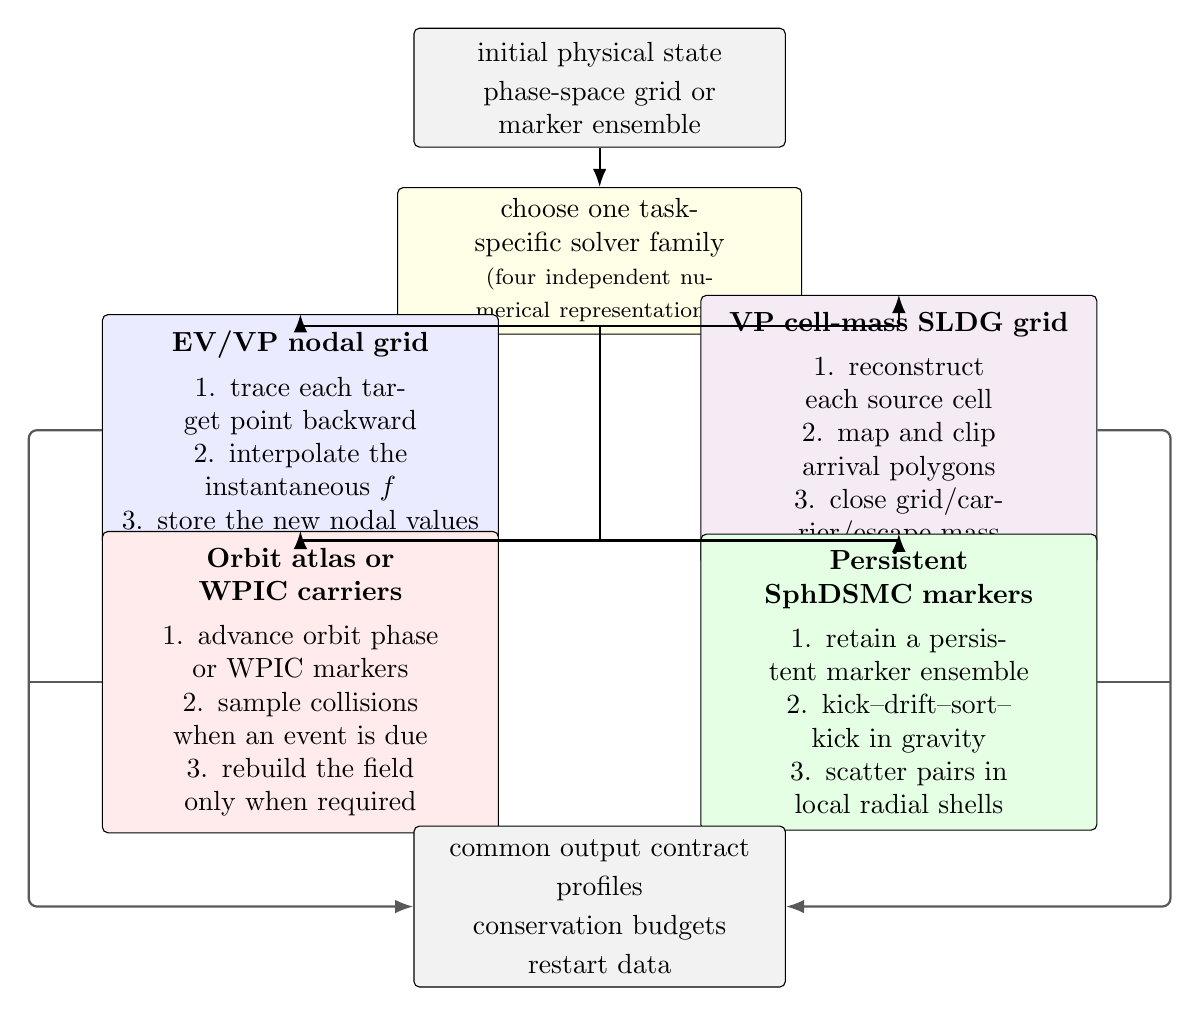
\begin{tikzpicture}[
  >=Latex,
  flow/.style={
    draw,
    rounded corners=2pt,
    align=center,
    inner sep=6pt,
    text width=0.38\textwidth,
    minimum height=2.35cm
  },
  state/.style={
    draw,
    rounded corners=2pt,
    align=center,
    inner sep=5pt,
    text width=0.36\textwidth
  },
  choice/.style={
    draw,
    rounded corners=2pt,
    align=center,
    inner sep=4pt,
    text width=0.40\textwidth,
    fill=yellow!10
  }
]
  \node[state,fill=gray!10] (initial) at (0,6.75)
    {initial physical state\\[2pt]
     phase-space grid or marker ensemble};

  \node[choice] (choice) at (0,4.55)
    {choose one task-specific solver family\\
     \footnotesize(four independent numerical representations)};

  \node[flow,fill=blue!8] (nodal) at (-3.8,2.4)
    {\textbf{EV/VP nodal grid}\\[4pt]
     1. trace each target point backward\\
     2. interpolate the instantaneous \(f\)\\
     3. store the new nodal values};

  \node[flow,fill=violet!8] (sldg) at (3.8,2.4)
    {\textbf{VP cell-mass SLDG grid}\\[4pt]
     1. reconstruct each source cell\\
     2. map and clip arrival polygons\\
     3. close grid/carrier/escape mass};

  \node[flow,fill=red!8] (kinetic) at (-3.8,-0.8)
    {\textbf{Orbit atlas or WPIC carriers}\\[4pt]
     1. advance orbit phase or WPIC markers\\
     2. sample collisions when an event is due\\
     3. rebuild the field only when required};

  \node[flow,fill=green!10] (dsmc) at (3.8,-0.8)
    {\textbf{Persistent SphDSMC markers}\\[4pt]
     1. retain a persistent marker ensemble\\
     2. kick--drift--sort--kick in gravity\\
     3. scatter pairs in local radial shells};

  \node[state,fill=gray!10] (output) at (0,-3.65)
    {common output contract\\[2pt]
     profiles\\[2pt]
     conservation budgets\\[2pt]
     restart data};

  % The central spine fans out through the open gaps between boxes.  In
  % particular, no connector passes through another representation family.
  \coordinate (topfork) at (0,3.72);
  \coordinate (lowerfork) at (0,1.00);
  \draw[->,thick] (initial.south) -- (choice.north);
  \draw[thick] (choice.south) -- (topfork) -- (lowerfork);
  \draw[->,thick] (topfork) -| (nodal.north);
  \draw[->,thick] (topfork) -| (sldg.north);
  \draw[->,thick] (lowerfork) -| (kinetic.north);
  \draw[->,thick] (lowerfork) -| (dsmc.north);

  % Each branch returns through an outside gutter before entering the common
  % output box.  The gutters make the fan-in explicit without crossing boxes.
  \coordinate (leftmerge) at (-7.25,-2.30);
  \coordinate (rightmerge) at (7.25,-2.30);
  \draw[thick,gray!70!black,rounded corners=3pt]
    (nodal.west) -- (-7.25,2.4) -- (leftmerge);
  \draw[thick,gray!70!black] (kinetic.west) -- (-7.25,-0.8);
  \draw[->,thick,gray!70!black,rounded corners=3pt]
    (leftmerge) |- (output.west);
  \draw[thick,gray!70!black,rounded corners=3pt]
    (sldg.east) -- (7.25,2.4) -- (rightmerge);
  \draw[thick,gray!70!black] (dsmc.east) -- (7.25,-0.8);
  \draw[->,thick,gray!70!black,rounded corners=3pt]
    (rightmerge) |- (output.east);
\end{tikzpicture}
\caption{Four alternative numerical representation families in the CPU tree.
A task-specific executable selects exactly one colored branch: nodal EV/VP
evaluates \(f\) at departure points, cell-integrated SLDG maps source-cell
mass, orbit/WPIC solvers carry persistent phase-space carriers, and SphDSMC
carries persistent spherical markers.  The numbered lines give the update
order within a branch.  The branches meet only at their common diagnostic and
restart products; there is no numerical flow from one colored box to another.}
\label{fig:venus-algorithm-overview}
\end{figure}
\else
The persistent-marker algorithms are:
\begin{enumerate}
\item Newtonian WPIC, including collisionless transport, elastic self-
interaction and Plummer gravitational scattering, unequal-weight subhalo
scattering/capture, event clocks, restarts, and marker-resolution limits;
\item persistent-marker SphDSMC, including radial sorting, enclosed gravity,
orbit integration, mean-free-path shells, parallel radix sorting, and local
finite-angle scattering;
\item the common physical mass, energy, locality, and escape diagnostics.
\end{enumerate}
The flowchart at the start of each module is the recommended first overview.
The governing equations and numerical update come next, followed by the run
block and then the detailed source excerpts used to interpret or modify the
calculation.
\fi

\subsection{Common Phase-Space Layout, Quadrature, and Grids}

The basic phase-space array is stored in row-major order as
\[
  f_{ijk}=f(r_i,w_j,L_k),\qquad
  q(i,j,k)=(iN_w+j)N_L+k .
\]
Here \(i\), \(j\), and \(k\) label the radial, radial-momentum, and angular-
momentum nodes; \(N_w\) and \(N_L\) are the total numbers of nodes in the last
two directions.  The function \(q(i,j,k)\) is the zero-based, one-dimensional
storage offset of \(f_{ijk}\) in the flattened array.
The indexing function is in \path{cpu/include/ev/grids.hpp}:
\codesource{All CPU grid EV, VP, and BP task executables}
  {\path{cpu/include/ev/grids.hpp}}
  {Row-major phase-space indexing used by the shared solver kernels}
\begin{lstlisting}[language=C++]
inline std::size_t idx(int i, int j, int k,
                       const Params& p) {
  return (static_cast<std::size_t>(i) * p.Nw + j) * p.NL + k;
}
\end{lstlisting}

The radial grid can be logarithmic, linear, piecewise-linear, or a custom grid
read from binary initial data.  The code stores the physical coordinate
\(r_i\) together with trapezoid weights. These weights assign each node the
width of its neighboring half-intervals. Applying the same rule to radial
integrals and \(w,L\) moment integrals keeps the density, enclosed mass,
and other moments on a consistent quadrature.  For
any ordered one-dimensional grid \(x_0,\ldots,x_{N-1}\), \(N\) is the number
of nodes and \(Q_i\) is the integration weight multiplying the value at node
\(x_i\):
\[
  Q_0=\frac{1}{2}(x_1-x_0),\quad
  Q_i=\frac{1}{2}(x_{i+1}-x_{i-1}),\quad
  Q_{N-1}=\frac{1}{2}(x_{N-1}-x_{N-2}).
\]
The implementation is in \path{cpu/include/ev/grids.hpp}:
\codesource{All CPU grid EV, VP, and BP task executables}
  {\path{cpu/include/ev/grids.hpp}}
  {Shared trapezoidal-quadrature implementation excerpt}
\begin{lstlisting}[language=C++]
inline std::vector<double> trapezoid_weights(
    const std::vector<double>& x) {
  const int n = static_cast<int>(x.size());
  std::vector<double> q(n, 0.0);
  q.front() = 0.5 * (x[1] - x[0]);
  q.back() = 0.5 * (x[n - 1] - x[n - 2]);
  for (int i = 1; i + 1 < n; ++i) {
    q[i] = 0.5 * (x[i + 1] - x[i - 1]);
  }
  return q;
}
\end{lstlisting}

\ifvenusfullcpu
The adaptive \(w\)-grid option uses a conservative remap.  When active matter
approaches either \(w\)-edge, the code chooses a larger symmetric interval,
constructs the new grid, and remaps each \((r,L)\) slice by conserving the
cell integral in \(w\).  The schematic displays the trigger and expansion.
\begin{figure}[ht]
\centering
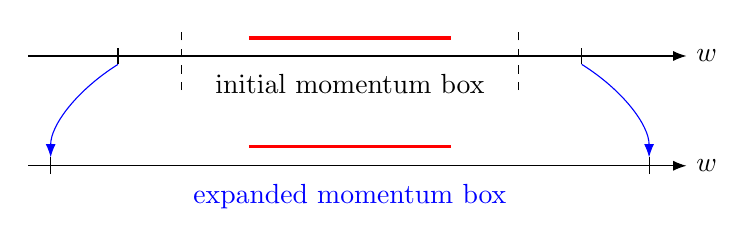
\begin{tikzpicture}[x=0.95cm,y=0.82cm,>=Latex]
  \draw[->] (-4.3,1.15) -- (4.5,1.15) node[right] {\(w\)};
  \draw (-3.1,1.02) -- (-3.1,1.28);
  \draw (3.1,1.02) -- (3.1,1.28);
  \draw[dashed] (-2.25,0.62) -- (-2.25,1.58);
  \draw[dashed] (2.25,0.62) -- (2.25,1.58);
  \draw[red,very thick] (-1.35,1.43) -- (1.35,1.43);
  \node at (0.0,0.72) {initial momentum box};

  \draw[->] (-4.3,-0.55) -- (4.5,-0.55) node[right] {\(w\)};
  \draw (-4.0,-0.68) -- (-4.0,-0.42);
  \draw (4.0,-0.68) -- (4.0,-0.42);
  \draw[red,very thick] (-1.35,-0.25) -- (1.35,-0.25);
  \draw[blue,->] (-3.1,1.02) .. controls (-3.65,0.62) and (-4.0,0.08) .. (-4.0,-0.42);
  \draw[blue,->] (3.1,1.02) .. controls (3.65,0.62) and (4.0,0.08) .. (4.0,-0.42);
  \node[blue] at (0.0,-1.02) {expanded momentum box};
\end{tikzpicture}
\caption{Adaptive expansion of the radial-momentum domain.  The red interval
marks the occupied part of the distribution above the active-cell cutoff.  When
it passes the dashed trigger line, VENUS enlarges the \(w\)-box and remaps the
same distribution onto the new grid.}
\label{fig:adaptive-w}
\end{figure}
Every \(\code{adaptive_w_every}\) steps, VENUS computes
\[
  w_{\rm act}
  =
  \max\{|w_j|:\exists(i,k)\ {\rm with}\ f_{ijk}>f_{\rm cut}\},
  \qquad
  f_{\rm cut}=\max(f_{\rm floor}^{\rm abs},
                  f_{\rm floor}^{\rm rel}\max f).
\]
Expansion is triggered when
\[
  w_{\rm act}\ge \code{adaptive_w_trigger}\,w_{\max},
\]
and the proposed new half-width is
\[
  w_{\max}^{\rm new}
  =
  \max\!\left(
    \code{adaptive_w_growth}\,w_{\max},
    \code{adaptive_w_margin}\,w_{\rm act}
  \right),
\]
clipped to \(\code{adaptive_w_max}\) when that cap is positive.
The remap and trigger live in \path{cpu/include/ev/advection.hpp}.  The essential
mass-preserving form is:
\codesource{Grid EV, VP, and BP solvers with adaptive radial momentum}
  {\path{cpu/include/ev/advection.hpp}}
  {Shortened conservative momentum-remap excerpt}
\begin{lstlisting}[language=C++]
const double before = distribution_mass(f, g, p, local_L0);
conservative_energy_remap_w(f, g.w, w_new, p, local_L0);
const double after = distribution_mass(f, g_new, p, local_L0);
if (after > 0.0 && before > 0.0) {
  const double corr = before / after;
  for (double& value : f) value *= corr;
}
\end{lstlisting}
Adaptive \(w\) is useful for EV collapse or VP infall tests where the occupied
radial velocity range grows.  It should be disabled for tracer runs and for
carefully calibrated VP/BP comparisons where the output grids must
remain identical between runs.
\fi

\ifvenusfullcpu
\subsection{Numerical Scope and Scientific Limitations of the Eulerian Families}
\label{sec:eulerian-family-scope}

The CPU implementation offers three complementary Eulerian descriptions of
spherical kinetic evolution.  Each stores and transports the distribution in
a different form and treats phase-space boundaries accordingly.  The choice
therefore depends on the orbits, boundary fluxes, and collision processes that
the calculation must resolve.

Here \emph{Eulerian} means that the distribution is stored on a fixed
phase-space mesh, rather than carried by individual moving markers.  An
\emph{upwind} face flux takes its distribution value from the side of a cell
face from which the characteristic flow arrives; the first-order rule uses
the nearest stored value on that upstream side.

The canonical family uses \(\eta=L^2/2\), the angular-momentum coordinate;
\(H=\Phi(r)+w^2/2+\eta/r^2\), the one-particle Hamiltonian in a frozen
potential \(\Phi\); and \(\tau_{\rm orb}\in[0,1)\), the radial-orbit phase
normalized by one radial period.  The subscript distinguishes this orbit
phase from the Schwarzschild time \(\tau\) used in the relativistic chapters.
The canonical chapter denotes this normalized orbit phase by
\(\zeta_{\rm orb}\).  In a relativistic context, \(\tau\) denotes
Schwarzschild time.  The orbit atlas tabulates the represented bound orbit families.
An \emph{open packet} is a continuous phase-space carrier for matter that the
bound atlas cannot currently represent, such as an unbound or otherwise
unsupported orbit; VENUS retains and advances that matter instead of silently
discarding it.

\begin{center}
\footnotesize
\begin{tabular}{@{}>{\raggedright\arraybackslash}p{0.19\linewidth}
                  >{\raggedright\arraybackslash}p{0.38\linewidth}
                  >{\raggedright\arraybackslash}p{0.34\linewidth}@{}}
\toprule
Solver family & Numerical representation & Scientific limitations and suitable use \\
\midrule
Explicit finite volume &
Cell averages on the spherical \((r,w,L)\) or \((r,w,\eta)\) mesh, advanced
with first-order upwind radial and radial-velocity face fluxes.  The
implementation includes reflecting, vacuum-outflow, and prescribed-inflow
faces, threaded flux construction, and a multidimensional CFL limit. &
The first-order stencil is diffusive near sharp orbit boundaries.  Long-time
equilibria require mesh refinement in every occupied phase-space direction,
and boundary fluxes must be included explicitly in mass and energy budgets. \\
\addlinespace
Grid semi-Lagrangian &
Nodal characteristic pullback for EV and VP, plus cell-integrated
conservative and Hamiltonian SLDG for VP.  The conservative path uses
positivity-limited reconstruction, mapped-cell overlap integrals, midpoint
self-gravity, recursive map refinement, and a delayed central carrier. &
The nodal path is not locally conservative.  The cell-integrated Hamiltonian
path is restricted to a static background, and very low angular momentum,
long delayed returns, rapidly changing fields, and map fallbacks require
problem-specific refinement. \\
\addlinespace
Canonical orbit phase &
A bound-orbit atlas in \((\eta,H,\tau_{\rm orb})\), frozen-potential phase translation,
Eulerian overlap maps, field rebuilds, finite-angle collision couplings, open
packets, positive packet compression, independent event clocks, and
versioned restarts. &
The representation is most efficient when the potential changes slowly
compared with an orbital period.  Unbound tails remain explicit packets, and
the orbit atlas, continuous-packet population, collision locality, and field
refresh cadence must all be refined together. \\
\bottomrule
\end{tabular}
\end{center}

For the finite-volume update, a cell \((i,j,k)\) loses the difference of its
two radial-face fluxes and its two radial-velocity-face fluxes.  This is a
conservative balance law: a reflecting face returns the appropriate
velocity-space flux, while an outflow or prescribed-inflow face contributes
to the recorded boundary budget.  Adding the interior matter to those
boundary transfers gives the conserved total.  This complete budget is the
quantity to check after each step.

The conservative SLDG family replaces face fluxes by a forward map of each
source cell.  It limits a local polynomial to remain nonnegative, subdivides
a mapped patch when its area or reversibility defect is too large, integrates
exact polynomial moments over polygon--cell intersections, and records mass
that cannot be represented by the accepted map.  Midpoint gravity and the
persistent delayed-inner carrier keep field evolution and unresolved central
passages in the same conservative accounting.  These ingredients are
described in detail in Section~\ref{sec:cell-integrated-sldg}.

The canonical family changes coordinates instead.  For a frozen spherical
potential, angular momentum \(\eta\), Hamiltonian \(H\), and orbital phase
\(\tau_{\rm orb}\) separate stationary orbit structure from phase translation.  Matter
created by a collision is retained as a continuous packet until it can be
mapped positively onto the orbit atlas; bound and open-orbit matter are never
silently conflated.  The full construction is described in
Section~\ref{sec:fully-kinetic-bp}.

All three families require a numerical convergence study appropriate to the
chosen physical problem.  Refine every coordinate or sampling budget that
controls the active operator; compare density, force, characteristic
invariants, and collision moments; reduce the timestep and any operator
splitting interval; verify that boundary and hidden-carrier ledgers close;
and compare uninterrupted and restarted evolution.  Supported OpenMP and MPI
layouts should reproduce the same physical observables within the declared
floating-point and stochastic uncertainty.  For collisional calculations,
also require collision regions smaller than the local mean free path and
separate Monte--Carlo scatter from deterministic discretization error.


\subsection{Einstein--Vlasov Equations}

\begin{figure}[htbp]
\centering
\textbf{Physics flow: grid-based Einstein--Vlasov semi-Lagrangian module}
\par\smallskip
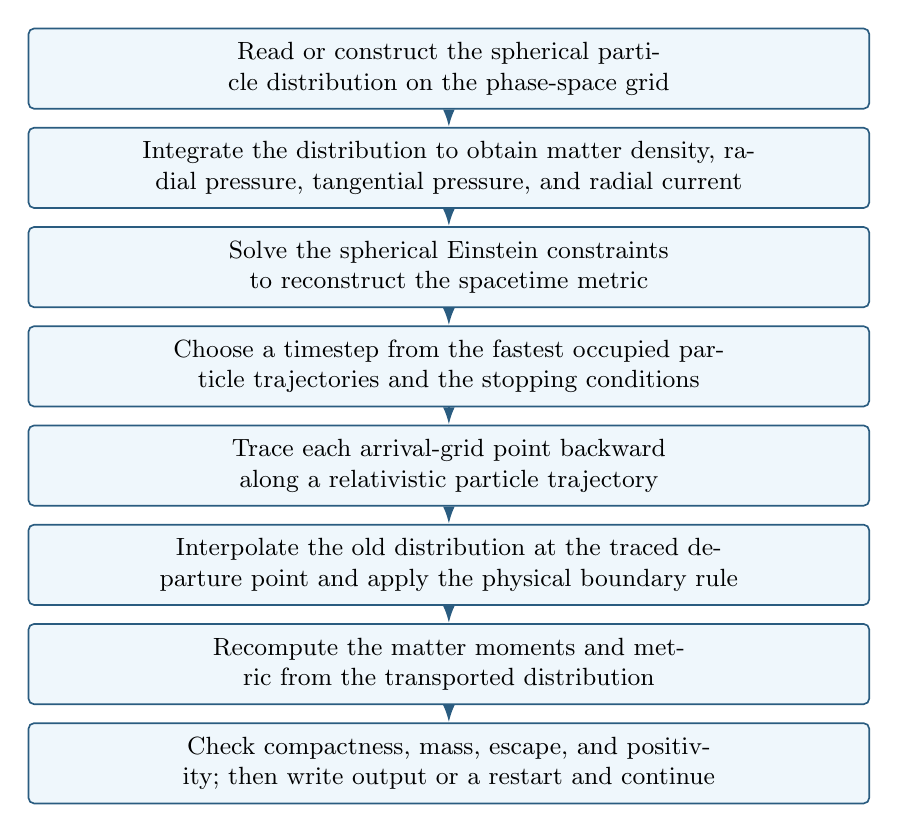
\begin{tikzpicture}[node distance=0.22cm]
\node[physicsflow] (ev1) {Read or construct the spherical particle distribution on the phase-space grid};
\node[physicsflow,below=of ev1] (ev2) {Integrate the distribution to obtain matter density, radial pressure, tangential pressure, and radial current};
\node[physicsflow,below=of ev2] (ev3) {Solve the spherical Einstein constraints to reconstruct the spacetime metric};
\node[physicsflow,below=of ev3] (ev4) {Choose a timestep from the fastest occupied particle trajectories and the stopping conditions};
\node[physicsflow,below=of ev4] (ev5) {Trace each arrival-grid point backward along a relativistic particle trajectory};
\node[physicsflow,below=of ev5] (ev6) {Interpolate the old distribution at the traced departure point and apply the physical boundary rule};
\node[physicsflow,below=of ev6] (ev7) {Recompute the matter moments and metric from the transported distribution};
\node[physicsflow,below=of ev7] (ev8) {Check compactness, mass, escape, and positivity; then write output or a restart and continue};
\draw[physicsarrow] (ev1) -- (ev2);
\draw[physicsarrow] (ev2) -- (ev3);
\draw[physicsarrow] (ev3) -- (ev4);
\draw[physicsarrow] (ev4) -- (ev5);
\draw[physicsarrow] (ev5) -- (ev6);
\draw[physicsarrow] (ev6) -- (ev7);
\draw[physicsarrow] (ev7) -- (ev8);
\end{tikzpicture}
\end{figure}

The EV module uses the Schwarzschild metric
\[
  \dd s^2=-e^{2\mu(\tau,r)}\dd\tau^2
           +e^{2\lambda(\tau,r)}\dd r^2+r^2\dd\Omega^2 .
\]
Here \(\tau\) is Schwarzschild time, \(r\) is areal radius, \(\mu\) is the
lapse potential, and \(\lambda\) is the radial metric potential.  This use of
\(\tau\) follows the manual-wide convention and distinguishes Schwarzschild
time from the EF advanced time \(v\).
The distribution is spherically symmetric in \((r,w,L)\), and the particle
energy is
\[
  \epsilon(r,w,L)=\sqrt{1+w^2+L^2/r^2}.
\]
The moments integrated from \(f\) are
\[
\begin{aligned}
  \rho_i &= \frac{2\pi}{r_i^2}\int\!\!\int
     \epsilon f\,L\,dL\,dw,\\
  p_i &= \frac{2\pi}{r_i^2}\int\!\!\int
     \frac{w^2}{\epsilon} f\,L\,dL\,dw,\\
  p_{T,i} &= \frac{2\pi}{r_i^2}\int\!\!\int
     \frac{L^2/r_i^2}{\epsilon} f\,L\,dL\,dw,\\
  j_i &= \frac{2\pi}{r_i^2}\int\!\!\int
     w f\,L\,dL\,dw .
\end{aligned}
\]
Here \(\rho\) is energy density, \(p\) is radial pressure, \(p_T\) is the
sum of the two tangential pressure components, and \(j\) is radial momentum
density.  The symbol \(\epsilon\) is the relativistic particle energy per unit
rest mass; the code uses units with particle rest mass and the speed of light
equal to one.
The local implementation, including the OpenMP reduction over the flattened
\((r,w,L)\) cell set, is in \path{cpu/include/ev/moments.hpp}:
\codesource{\code{venus_cpu_einstein_vlasov_eulerian}}
  {\path{cpu/include/ev/moments.hpp}}
  {Shortened relativistic-moment kernel excerpt}
\begin{lstlisting}[language=C++]
const double eps =
    std::sqrt(1.0 + w[j] * w[j] + (LL / r[i]) * (LL / r[i]));
const double weight = wq[j] * Lq[k] * LL * f[idx(i, j, k, p)];
srho += eps * weight;
sp   += (w[j] * w[j] / eps) * weight;
sj   += w[j] * weight;
out.rho[i] = 2.0 * pi / (r[i] * r[i]) * srho;
out.p[i]   = 2.0 * pi / (r[i] * r[i]) * sp;
out.j[i]   = 2.0 * pi / (r[i] * r[i]) * sj;
\end{lstlisting}
\subsection{Einstein--Vlasov Metric Reconstruction}

At each step, the matter moments supply the radial Einstein constraints.
Integrating the density outward gives the enclosed mass, which determines
the radial metric. The radial pressure then enters the lapse equation.  With \(m_r=4\pi r^2\rho\),
\[
  m(r_i)\simeq \frac{4\pi}{3}\rho_0 r_0^3
    +4\pi\int_{r_0}^{r_i} r^2\rho(r)\,dr ,
\]
\[
  e^{-2\lambda}=1-\frac{2m}{r},\qquad
  \mu_r=e^{2\lambda}\left(\frac{m}{r^2}+4\pi r p\right).
\]
Let \(M=m(r_{\max})\) denote the total mass enclosed by the outer radial grid
point.  The outer boundary condition is asymptotically Schwarzschild:
\[
  \mu(r_{\max})=\frac{1}{2}\log\!\left(1-\frac{2M}{r_{\max}}\right),
\]
and \(\mu\) is integrated inward by the trapezoid rule.  The implementation is
in \path{cpu/include/ev/metric.hpp}:
\codesource{\code{venus_cpu_einstein_vlasov_eulerian}}
  {\path{cpu/include/ev/metric.hpp}}
  {Shortened Schwarzschild metric reconstruction excerpt}
\begin{lstlisting}[language=C++]
m[i] = m[i - 1] + 4.0 * pi * 0.5 *
    (y[i - 1] + y[i]) * (r[i] - r[i - 1]);
const double gap = 1.0 - 2.0 * m[i] / r[i];
lambda[i] = -0.5 * std::log(gap);
mu_r[i] = std::exp(2.0 * lambda[i]) *
    (m[i] / (r[i] * r[i]) + 4.0 * pi * r[i] * mom.p[i]);
mu[p.Nr - 1] = 0.5 * std::log(std::max(1.0 - 2.0 * m[p.Nr - 1] / r.back(), tiny));
for (int i = p.Nr - 2; i >= 0; --i) {
  mu[i] = mu[i + 1] - 0.5 * (mu_r[i + 1] + mu_r[i]) *
      (r[i + 1] - r[i]);
}
\end{lstlisting}
The compactness gap \(1-2m/r\) is monitored in \code{history.csv}.  A small
gap is the numerical signal of approach to trapped-surface or horizon
formation in this coordinate system.

The polar-time derivative of the radial metric potential is reconstructed
from the radial current:
\[
 \lambda_\tau=-4\pi r\,e^{\lambda+\mu}j.
\]
This quantity enters the momentum characteristic during the frozen step and
supplies the relativistic momentum change caused by time-dependent geometry.
The C++ member \code{lambda_t} stores this \(\lambda_\tau\); its historical
\code{_t} suffix does not introduce a different time coordinate.

\subsection{Einstein--Vlasov Characteristics and Leap-Frog Step}
\label{sec:ev-semi-lagrangian}

The EV transport equation is solved by following characteristics.  In the
variables used by the code,
\[
  \frac{dr}{d\tau}=e^{\mu-\lambda}\frac{w}{\epsilon},
\]
\[
  \frac{dw}{d\tau}= -\lambda_\tau w
  -e^{\mu-\lambda}\mu_r\epsilon
  +e^{\mu-\lambda}\frac{L^2}{r^3\epsilon}.
\]
The timestep limits the distance a characteristic crosses in radius and
momentum during one update. A CFL safety factor reduces the corresponding
crossing times, and optional user ceilings can shorten the result.  The scan is in \path{cpu/include/ev/timestep.hpp}:
\codesource{\code{venus_cpu_einstein_vlasov_eulerian}}
  {\path{cpu/include/ev/timestep.hpp}}
  {Shortened characteristic-speed timestep scan}
\begin{lstlisting}[language=C++]
const double vr = std::exp(met.mu[i] - met.lambda[i]) * w[j] / eps;
const double accel = -met.lambda_t[i] * w[j]
  - std::exp(met.mu[i] - met.lambda[i]) * met.mu_r[i] * eps
  + std::exp(met.mu[i] - met.lambda[i]) * LL * LL /
      (r[i] * r[i] * r[i] * eps);
local_min = std::min(local_min, cfl * dr / std::max(std::abs(vr), tiny));
local_min = std::min(local_min, cfl * dw / std::max(std::abs(accel), tiny));
\end{lstlisting}
With the metric frozen over one timestep, define
\[
  v(r,w,L)=e^{\mu-\lambda}\frac{w}{\epsilon},\qquad
  a(r,w,L)=
  -\lambda_\tau w-e^{\mu-\lambda}\mu_r\epsilon
  +e^{\mu-\lambda}\frac{L^2}{r^3\epsilon}.
\]
For the default \code{semi_lagrangian_kick_drift_kick} integrator, the
backward footpoint for target cell \((r_i,w_j,L_k)\) is
\begin{align}
  w_{1/2} &= w_j-\frac{\Delta\tau}{2}a(r_i,w_j,L_k),\\
  r_{\rm dep} &= r_i-\Delta\tau\,v(r_i,w_{1/2},L_k),\\
  w_{\rm dep} &= w_{1/2}
    -\frac{\Delta\tau}{2}a(r_{\rm dep},w_{1/2},L_k).
\end{align}
Radial reflection is applied after the drift and after the second kick.  The
metric in the second kick is sampled at \(r_{\rm dep}\).  The distribution is
then pulled back by fixed-\(L\) interpolation.  Here
\(I_{r,w}[f](r_*,w_*;L_k)\) denotes the configured two-dimensional
interpolation of \(f\) at \((r_*,w_*)\) on the fixed \(L_k\) slice; the
bilinear form used by the direct nodal path is written explicitly below.
\[
  f^{n+1}_{ijk}
  =
  I_{r,w}\!\left[f^n(\cdot,\cdot,L_k)\right]
  (r_{\rm dep},w_{\rm dep}).
\]
These explicit kicks and drift form a first-order characteristic method for
the general relativistic equations, whose radial speed and momentum rate
both depend on \(r,w\).  The familiar second-order KDK result applies when
the kick and drift are exact subflows of a separable Hamiltonian, as in the
Newtonian construction above.  Freezing the old metric over a full
self-consistent grid step also gives first-order time coupling.  Selecting
a higher-order characteristic solver improves the frozen-field trajectory;
time-centering the evolving field is a separate requirement.  The code
writes mass and boundary-loss diagnostics to measure its interpolation
transport budget.
The implementation is in \path{cpu/include/ev/advection.hpp}:
\codesource{\code{venus_cpu_einstein_vlasov_eulerian}}
  {\path{cpu/include/ev/advection.hpp}}
  {Shortened backward-characteristic pullback excerpt}
\begin{lstlisting}[language=C++]
const CharacteristicState dep = trace_ev_characteristic_footpoint(
    r[i], w[j], Lk, x_r, r, metric, dt, p, integrator_plan);
f_new[idx(i, j, k, p)] =
    std::max(0.0, interpolate_slice(f, dep.r, dep.w, k, x_r, r, w, p));
\end{lstlisting}
The radial origin and outer boundary are treated with reflection/escape logic
depending on the configured boundary mode.  The same file contains the escape
diagnostic written to \code{history.csv}.

\subsubsection{What ``semi-Lagrangian'' means in the EV solver}

The collisionless Vlasov equation states that the scalar distribution is
constant along a particle characteristic:
\[
 \frac{\dd f}{\dd \tau}
 =\partial_\tau f+\dot r\,\partial_r f+\dot w\,\partial_w f=0,
 \qquad \dot L=0.
\]
Consequently, a target point \((r_i,w_j,L_k)\) at \(\tau^{n+1}\) has the
value carried from its departure point at \(\tau^n\):
\[
 f^{n+1}(r_i,w_j,L_k)
 =f^n(r_{\rm dep},w_{\rm dep},L_k).
\]
The term \emph{Lagrangian} refers to following the orbit; the prefix
\emph{semi} indicates that the distribution is still stored on a fixed grid
and is interpolated at the off-grid departure point.  No particle-marker state
is used by this existing Einstein--Vlasov solver.

The angular momentum \(L\) is conserved exactly by spherical symmetry, so
each \(L_k\) slice can be transported independently.

\subsubsection{Metric and distribution time levels}

At the beginning of one EV step, VENUS computes moments from \(f^n\) and solves
the radial Einstein constraints for
\[
 {\cal G}^n=\{\mu^n,\lambda^n,\mu_r^n,\lambda_\tau^n\}.
\]
The metric set \({\cal G}^n\) is frozen while every target point traces
backward over \(\Delta\tau\).  Once the pullback has produced \(f^{n+1}\), time
and step are advanced; moments and a new metric are computed at the top of the
next loop.  In code order:
\codesource{\code{venus_cpu_einstein_vlasov_eulerian}}
  {\path{cpu/include/ev/solver_evolution.hpp} with kernels in
   \path{cpu/include/ev/moments.hpp}, \path{cpu/include/ev/metric.hpp},
   \path{cpu/include/ev/timestep.hpp}, and \path{cpu/include/ev/advection.hpp}}
  {Abbreviated macrostep pseudocode; it is not a literal contiguous source block}
\begin{lstlisting}[language=C++]
Moments moments = compute_global_moments(f_n, ...);
Metric metric_n = solve_metric(moments, r, p);
double dt = choose_dt(f_n, r, w, L, metric_n, ...);
f_np1 = advect(f_n, x_r, r, w, L, metric_n, dt, p);
\end{lstlisting}
The characteristic solve uses one metric during a macrostep. Reconstructing
the metric from the transported matter at the next step supplies the
self-consistent time evolution of the spacetime.

\subsubsection{Radial coordinate interpolation}

The numerical radial coordinate is
\[
 x_r=
 \begin{cases}
  \ln r,&\code{radial_grid = log},\\
  r,&\text{linear or piecewise-linear coordinate}.
 \end{cases}
\]
Metric profiles are linearly interpolated in \(x_r\), not necessarily in
physical radius.  For a departure radius \(r_{\rm dep}\), let
\(x_{\rm dep}=x_r(r_{\rm dep})\), and let
\[
 \xi=\frac{x_{\rm dep}-x_i}{x_{i+1}-x_i},
 \qquad
 \zeta=\frac{w_{\rm dep}-w_j}{w_{j+1}-w_j}.
\]
The fixed-\(L_k\) bilinear pullback is
\[
 \begin{split}
 I_{r,w}[f]={}&(1-\xi)(1-\zeta)f_{i,j,k}
 +\xi(1-\zeta)f_{i+1,j,k}\\
 &+(1-\xi)\zeta f_{i,j+1,k}
 +\xi\zeta f_{i+1,j+1,k}.
 \end{split}
\]
If the departure point lies outside an outflow radial or momentum boundary,
the interpolated value is zero.  The final value is protected by
\(\max(0,I_{r,w}[f])\), which prevents a tiny negative roundoff value but is
not a conservative positivity redistribution.

\subsubsection{Inner and outer radial boundaries}

The boundary choices distinguish a finite reflecting wall, the regular
spherical origin, vacuum outflow, and prescribed Newtonian inflow.  The
conservative grid solver also supports delayed return through an unresolved
central region, as described in its transport section.

A finite wall has a fixed physical radius \(R\).  For the Newtonian solver,
the physical radial velocity is \(\dot r=Hr+w\), where \(w\) is the stored
peculiar velocity.  Specular reflection reverses \(\dot r\) at the wall.
It therefore gives
\begin{equation}
 r=R:\qquad w_{\rm out}=-w_{\rm in}-2H(t_{\rm hit})R,
 \qquad HR+w_{\rm out}=-(HR+w_{\rm in}),
 \label{eq:fixed-physical-wall}
\end{equation}
Here \(t_{\rm hit}\) is the wall-crossing time. The KDK orbit solver locates
this crossing within its free angular drift, reverses the physical radial
velocity there, and advances the remaining interval. Its implementation is
derived in Section~\ref{sec:wpic-expanding-kdk}. In a static
Newtonian calculation \(H=0\).  For the Schwarzschild-coordinate solver,
\(w\) is radial momentum in the local orthonormal frame and the finite-wall
reflection also changes its sign.

For boundary interpolation and stage projection, the extended radius
\(r'=2R-r\) and velocity \(w'=-w-2HR\) obey
\(Hr'+w'=-(Hr+w)\). The shared outer-wall extension is
\codesource{Fixed physical radial wall}
{\path{cpu/include/ev/advection.hpp}}
{Extend a boundary value by reflecting radius and physical radial velocity}
\begin{lstlisting}[language=C++]
if (rp > r_max) {
    rp = r_max - (rp - r_max);
    wp = -wp - 2.0 * hubble * r_max;
}
\end{lstlisting}
The inner wall uses the same map with \(R=r_{\min}\).  Multiple crossings
are permitted within the bounded reflection loop.  An endpoint that remains
outside the permitted radial domain raises an error and requires a shorter
step.

At the true origin the parity map is
\begin{equation}
 r<0:\qquad r\leftarrow-r,\qquad w\leftarrow-w.
 \label{eq:origin-parity-map}
\end{equation}
The regular distribution obeys \(f(-r,-w,L)=f(r,w,L)\).  At a positive
radius, it can have a nonzero radial current.  The pointwise pullback
therefore symmetrizes the first radial plane only for a finite reflecting
wall.  Its incoming velocity is paired with \(-w-2Hr_{\min}\).  With
\code{inner_boundary=origin_parity}, the characteristic crossing supplies
the parity condition at \(r=0\).

Vacuum outflow permits an outgoing characteristic to leave the radial or
momentum domain.  Its escaped mass is part of the conservation budget.
The Newtonian prescribed-inflow option supplies the configured distribution
to incoming outer characteristics.  The Eddington--Finkelstein solver uses
vacuum outflow at its outer boundary; its inner excision condition is
determined by the local null directions, as described in the relativistic
WPIC section.

\paragraph{Prescribed incoming mass.}
For a Newtonian inflow pulse, let \(s>0\) be its prescribed inward mean
speed, \(\sigma\) its radial velocity dispersion, and
\(u=Hr+w\) the physical radial velocity.  The radial Gaussian is centered
at \(u=-s\).  Only its incoming half crosses the outer face.  Its flux is
therefore normalized by
\begin{equation}
 \int_{-\infty}^{0}(-u)\,
 \frac{e^{-(u+s)^2/(2\sigma^2)}}{\sqrt{2\pi}\sigma}\,du
 =\frac{s}{2}\operatorname{erfc}\!\left(-\frac{s}{\sqrt{2}\sigma}\right)
  +\frac{\sigma}{\sqrt{2\pi}}e^{-s^2/(2\sigma^2)}.
 \label{eq:incoming-gaussian-flux}
\end{equation}
The Gaussian pulse in time is truncated at the configured number of standard
deviations \(c\).  Dividing it by \(\operatorname{erf}(c/\sqrt{2})\)
preserves its unit time integral.  The prescribed shell mass divided by
\(4\pi R^2\) and the right-hand side of
 equation~\eqref{eq:incoming-gaussian-flux} then gives the density amplitude.
The tangential distribution is normalized separately with the spherical
velocity measure.  Integrating the incoming flux over the full pulse gives
the requested shell mass.  A finite velocity grid or a time interval covering
only part of the pulse supplies the corresponding partial mass.
\codesource{Incoming Gaussian flux normalization}
{\path{cpu/include/ev/vlasov_poisson.hpp}}
{Normalize the incoming radial flux and the truncated time envelope}
\begin{lstlisting}[language=C++]
const double z = speed / sigma_u;
const double incoming_speed =
    0.5 * speed * std::erfc(-z / std::sqrt(2.0))
    + sigma_u * std::exp(-0.5 * z * z)
      / std::sqrt(2.0 * PI);
const double time_normalization =
    std::erf(p.vp_inflow_time_cutoff / std::sqrt(2.0));
\end{lstlisting}

\subsubsection{CFL limit in logarithmic and linear radius}

Let \(v_r=\dot r\) and \(a_w=\dot w\).  On a logarithmic radial coordinate,
the characteristic speed is
\[
 \dot x_r=\frac{\dot r}{r};
\]
on a linear coordinate it is simply \(\dot r\).  VENUS scans only cells with
\[
 f_{ijk}>
 \max\!\left(f_{\rm active,abs},
 f_{\rm active,rel}\max f\right).
\]
If \(\Delta x_{r,\min}\) and \(\Delta w_{\min}\) are the smallest coordinate
spacings, the selected step is
\[
 \Delta\tau=\min\left[
 \Delta\tau_{\max},
 C_{\rm CFL}\frac{\Delta x_{r,\min}}{\max|\dot x_r|},
 C_{\rm CFL}\frac{\Delta w_{\min}}{\max|\dot w|}
 \right].
\]
The maxima and active-cell count are reduced over threads and MPI ranks.
Cells below the activity floor do not set the timestep, but their mass is not
removed from the distribution.

\subsubsection{Transport budget and current numerical limitations}

Bilinear nodal pullback is not locally conservative.  VENUS therefore reports
the quadrature mass before and after transport and separately estimates mass
whose forward characteristic reaches the outer \(r\) or \(w\) boundaries.
The escape estimate is a warning based on active nodal cells; it is not an
exact finite-volume face flux.  Adaptive \(w\)-grid remapping can recover a
growing occupied velocity range, but its explicit mass normalization is also
a numerical remap and must be included in convergence studies.

The existing EV semi-Lagrangian path has these present properties:
\begin{itemize}
\item relativistic spherical characteristics with a freshly constrained metric
at the start of every macrostep;
\item KDK, explicit Runge--Kutta (RK), extrapolated midpoint, and
Adams--Bashforth (AB) characteristic solvers;
\item bilinear interpolation on each fixed-\(L\) slice;
\item finite-wall, origin-parity, reflecting-outer, and vacuum-outflow logic;
\item OpenMP/std::thread target-cell parallelism and MPI \(L\)-slab
decomposition;
\item distributed restarts, adaptive-\(w\) support for compatible workflows,
and phase/profile/escape diagnostics.
\end{itemize}
Its main numerical limitations are the nonconservative nodal interpolation,
first-step frozen metric rather than a time-centred metric predictor, and
reduced accuracy when a characteristic crosses a reflection or a strong
force variation within one large step.  These limitations are why mass,
boundary occupancy, compactness gap, timestep, and resolution refinement must
be monitored together.  The distinct weighted-marker Einstein--Vlasov WPIC
implementation, its relativistic marker equations, runner, restart contract,
tests, and completed low/high-compactness examples are documented in
Section~\ref{sec:weighted-einstein-vlasov-pic}.

\subsubsection{How to run the existing EV semi-Lagrangian solver}

\noindent\textbf{Runnable starting point.}
Save the first block as \path{params.ini}; parameters not shown retain their
documented defaults.
\codesource{\code{venus_cpu_einstein_vlasov_eulerian}}
  {\path{cpu/src/apps/einstein_vlasov/eulerian.cpp} and
   \path{cpu/include/ev/config.hpp}}
  {Example input for the nodal Schwarzschild EV task}
\begin{lstlisting}[basicstyle=\ttfamily\scriptsize]
# params.ini: grid-based Einstein--Vlasov semi-Lagrangian run
physics_model = einstein_vlasov
initial_data = analytic
shell_initial_df = true
gaussian_density_shell = true
Nr = 96
Nw = 96
NL = 24
r_min = 1e-2
r_max = 80
w_max = 5
L_max = 8
integrator = semi_lagrangian_kick_drift_kick
t_end = 1
cfl = 0.35
dt_max = 0.04
save_every = 10
output_dir = output/ev_semilagrangian_example
\end{lstlisting}
The literal input names \code{t_end} and \code{dt_max} are legacy,
module-generic keys; in this relativistic module they set the final
Schwarzschild time and the ceiling on \(\Delta\tau\), respectively.
From the \path{VENUS/cpu} directory, build and run it with:
\codesource{\code{venus_cpu_einstein_vlasov_eulerian}}
  {\path{cpu/Makefile} and
   \path{cpu/src/apps/einstein_vlasov/eulerian.cpp}}
  {Build and invocation commands}
\begin{lstlisting}[basicstyle=\ttfamily\scriptsize]
make cpu-task-solvers
./venus_cpu_einstein_vlasov_eulerian --config params.ini
\end{lstlisting}

The modular executable is:
\codesource{\code{venus_cpu_einstein_vlasov_eulerian}}
  {\path{cpu/src/apps/einstein_vlasov/eulerian.cpp} and \path{cpu/Makefile}}
  {Build and invocation commands}
\begin{lstlisting}
cd VENUS/cpu
make cpu-task-solvers
./venus_cpu_einstein_vlasov_eulerian \
  --config examples/einstein_vlasov_low_compactness_virialized_halo.ini \
  --output-dir output/ev_low_compactness
\end{lstlisting}
The compatibility executable runs an EV configuration through the older
self-contained source:
\codesource{\code{venus_einstein_vlasov_serial}}
  {\path{cpu/src/venus_einstein_vlasov.cpp} and \path{cpu/Makefile}}
  {Compatibility invocation; new work should use the task-specific executable above}
\begin{lstlisting}
./venus_einstein_vlasov_serial \
  --config examples/einstein_vlasov_low_compactness_virialized_halo.ini \
  --output-dir output/ev_compatibility
\end{lstlisting}
The defining parameter block is:
\codesource{\code{venus_cpu_einstein_vlasov_eulerian}}
  {\path{cpu/include/ev/config.hpp} and
   \path{cpu/src/apps/einstein_vlasov/eulerian.cpp}}
  {Minimal Schwarzschild EV configuration fragment}
\begin{lstlisting}
physics_model = einstein_vlasov
integrator = semi_lagrangian_kick_drift_kick
inner_boundary = reflecting
outer_boundary = outflow_vacuum
cfl = 0.35
dt_max = 0.04
\end{lstlisting}
For a high-order characteristic study, replace the integrator by
\code{semi_lagrangian_rk} and set
\code{time_integrator_order}; orders two through four use explicit RK
tableaus, while larger requested orders use extrapolated midpoint.  The
\code{semi_lagrangian_adams_bashforth} option is intended for smooth-field
timing and convergence experiments.

\subsection{Higher-Order Characteristic Integrators}

The higher-order characteristic integrators use the semi-Lagrangian pullback
with their selected footpoint ODE solver.  Let
\[
  y(\tau)=\begin{pmatrix}r(\tau)\\w(\tau)\end{pmatrix},\qquad
  \frac{dy}{d\tau}=F(y;L),
\]
where \(F=(v,a)\) is the frozen-field characteristic vector.  The footpoint is
obtained by integrating backward with \(h=-\Delta\tau\).

For \code{integrator = semi_lagrangian_rk} and
\(2\le\code{time_integrator_order}\le4\), VENUS uses precomputed explicit
Runge--Kutta tableaus:
\[
  Y_s=y_n+h\sum_{q<s}a_{sq}F(Y_q),\qquad
  y_{\rm dep}=y_n+h\sum_s b_s F(Y_s).
\]
For requested orders \(>4\), VENUS switches to an extrapolated modified
midpoint characteristic integrator.  For substep counts \(n_m\), define
\(\delta_m=h/n_m\) and compute
\[
  z_0=y_n,\qquad z_1=z_0+\delta_m F(z_0),\qquad
  z_{\ell+1}=z_{\ell-1}+2\delta_m F(z_\ell),
\]
\[
  M_m(h)=\frac{1}{2}\left[z_{n_m}+z_{n_m-1}
     +\delta_m F(z_{n_m})\right].
\]
The extrapolated footpoint is
\[
  y_{\rm dep}=\sum_m \omega_m M_m(h),\qquad
  \omega_m=\prod_{\ell\ne m}\frac{-x_\ell}{x_m-x_\ell},
  \qquad x_m=\frac{1}{n_m^2}.
\]
The number of levels is \(\lceil p/2\rceil\), so an odd requested order is
rounded up to the next even effective order.  The precomputed data live in
\path{cpu/include/ev/characteristic_integrators.hpp}.

For \code{integrator = semi_lagrangian_adams_bashforth}, VENUS uses
\[
  y_{m+1}=y_m+h\sum_{q=0}^{p-1}\beta_q F_{m-q},
\]
where the Adams--Bashforth weights are generated once from the Lagrange basis
on nodes \(0,-1,\ldots,-p+1\):
\[
  \beta_q=\int_0^1 \ell_q(s)\,ds,\qquad
  \ell_q(s)=\prod_{\substack{m=0\\m\ne q}}^{p-1}
  \frac{s+m}{-q+m}.
\]
Because each semi-Lagrangian target cell traces a fresh characteristic, the AB
history is built inside that trace using RK starter substeps.  This makes AB
valid for characteristic integration, but it is less robust than RK near
reflections or rapidly changing forces.  Use RK4 or the extrapolated midpoint
path for high-accuracy tests; use AB for smooth-field timing measurements.

\subsection{Vlasov--Poisson Equations}

\begin{figure}[htbp]
\centering
\textbf{Physics flow: nodal Vlasov--Poisson semi-Lagrangian module}
\par\smallskip
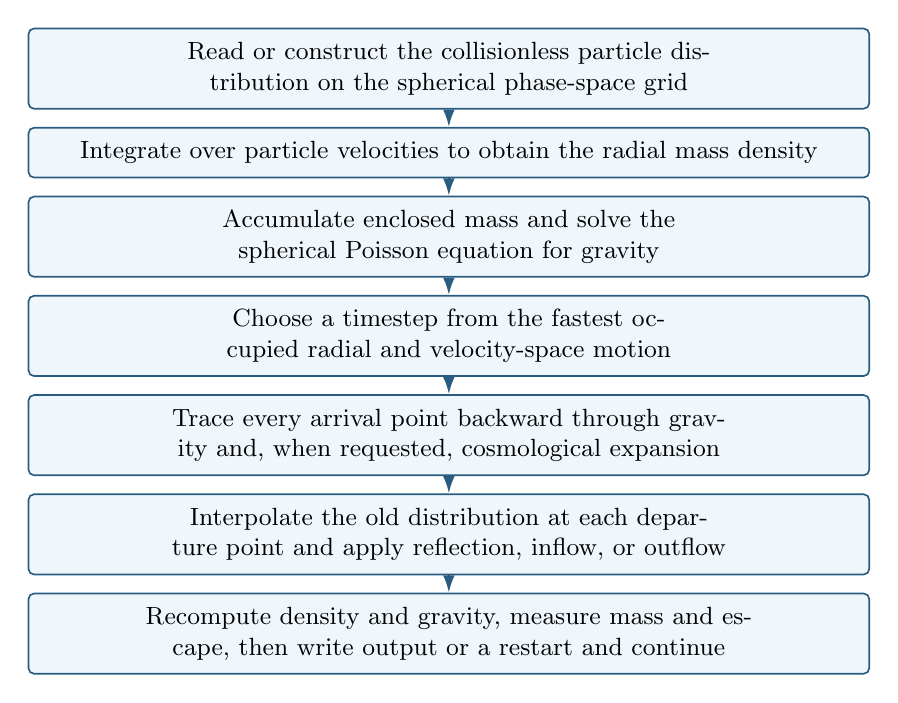
\begin{tikzpicture}[node distance=0.22cm]
\node[physicsflow] (vp1) {Read or construct the collisionless particle distribution on the spherical phase-space grid};
\node[physicsflow,below=of vp1] (vp2) {Integrate over particle velocities to obtain the radial mass density};
\node[physicsflow,below=of vp2] (vp3) {Accumulate enclosed mass and solve the spherical Poisson equation for gravity};
\node[physicsflow,below=of vp3] (vp4) {Choose a timestep from the fastest occupied radial and velocity-space motion};
\node[physicsflow,below=of vp4] (vp5) {Trace every arrival point backward through gravity and, when requested, cosmological expansion};
\node[physicsflow,below=of vp5] (vp6) {Interpolate the old distribution at each departure point and apply reflection, inflow, or outflow};
\node[physicsflow,below=of vp6] (vp7) {Recompute density and gravity, measure mass and escape, then write output or a restart and continue};
\draw[physicsarrow] (vp1) -- (vp2);
\draw[physicsarrow] (vp2) -- (vp3);
\draw[physicsarrow] (vp3) -- (vp4);
\draw[physicsarrow] (vp4) -- (vp5);
\draw[physicsarrow] (vp5) -- (vp6);
\draw[physicsarrow] (vp6) -- (vp7);
\end{tikzpicture}
\end{figure}

The static VP module solves
\[
  \partial_t f + w\,\partial_r f
  +\left(\frac{L^2}{r^3}-\partial_r\Phi\right)\partial_w f=0,
\]
with
\[
  \frac{1}{r^2}\partial_r(r^2\partial_r\Phi)=4\pi G\rho,\qquad
  \rho=\frac{2\pi}{r^2}\int\!\!\int f L\,dL\,dw .
\]
The expanding power-law FLRW form uses the configured scale factor \(a(t)\),
Hubble factor \(H(t)\), and either total-density or density-contrast Poisson
source.  The supplied expanding examples use the EdS value
\(\alpha=2/3\).  The helpers are in \path{cpu/include/ev/vlasov_poisson.hpp}:
\codesource{\code{venus_cpu_vlasov_poisson_eulerian}}
  {\path{cpu/include/ev/vlasov_poisson.hpp}}
  {Expanding-background helper excerpt}
\begin{lstlisting}[language=C++]
inline VpBackground vp_background(double t, const Params& p) {
  bg.tau = t + p.vp_time_offset;
  if (p.vp_universe == "expanding") {
    bg.H = p.vp_alpha / bg.tau;
    bg.a = std::pow(bg.tau / p.vp_time_offset, p.vp_alpha);
    bg.rho_bar = 3.0 * bg.H * bg.H / (8.0 * PI * p.vp_gravity);
  }
  return bg;
}
\end{lstlisting}
The radial Poisson solve is again a trapezoid integration of enclosed mass
followed by an inward integration of the force:
\codesource{\code{venus_cpu_vlasov_poisson_eulerian}}
  {\path{cpu/include/ev/vlasov_poisson.hpp}}
  {Shortened radial Poisson reconstruction excerpt}
\begin{lstlisting}[language=C++]
source_mass[i] = source_mass[i - 1] + 4.0 * pi * 0.5 *
    (y[i - 1] + y[i]) * (r[i] - r[i - 1]);
phi_r[i] = Gfac * source_mass[i] / (r[i] * r[i]);
phi[p.Nr - 1] = -Gfac * source_mass[p.Nr - 1] / r.back();
for (int i = p.Nr - 2; i >= 0; --i) {
  phi[i] = phi[i + 1] - 0.5 * (phi_r[i + 1] + phi_r[i]) *
      (r[i + 1] - r[i]);
}
\end{lstlisting}
The expanding solver stores physical radius \(r\) and peculiar radial
velocity \(w=\dot r-Hr\).  Consequently the local characteristic speeds are
\[
  \dot r = Hr+w,\qquad
  \dot w = \frac{L^2}{r^3}-\Phi_r-Hw ,
\]
with the static limit \(H=0\).  The scale factor \(a(t)\) determines
\(H=\dot a/a\) and the configured cosmological background, but it does not
divide these physical-coordinate characteristic speeds.  The implementation
is in the same header:
\codesource{\code{venus_cpu_vlasov_poisson_eulerian}}
  {\path{cpu/include/ev/vlasov_poisson.hpp}}
  {Radial characteristic-speed excerpt}
\begin{lstlisting}[language=C++]
const double vr = field.background.H * r[i] + w[j];
const double aw = L[k] * L[k] / (r[i] * r[i] * r[i])
  - field.phi_r[i] - field.background.H * w[j];
\end{lstlisting}

\subsection{Nodal Characteristic Transport and Interpolation}

The nodal collisionless solver stores \(f\) at the grid points
\((r_i,w_j,L_k)\).  During one semi-Lagrangian update it performs the
following operations:
\begin{enumerate}
\item Choose a target grid point \((r_i,w_j,L_k)\) at the new time.
\item Follow its orbit backward by one timestep to find the departure point
      \((r_{\rm d},w_{\rm d},L_k)\).
\item Locate the grid cells surrounding the departure point.
\item Interpolate the old distribution at that point.
\item Store the interpolated value at the target grid point.
\end{enumerate}

This procedure follows the characteristic identity
\[
 f(t+\Delta t,r_i,w_j,L_k)
 =f(t,r_{\rm d},w_{\rm d},L_k).                           \tag{VP1}
\]
A traced departure point generally lies between stored grid points.
Interpolation estimates the earlier distribution at that location, and the
characteristic identity carries that value to the arrival point.

\subsubsection{\texorpdfstring{Direct \((r,w)\) interpolation}{Direct (r,w) interpolation}}

The setting
\codesource{\code{venus_cpu_vlasov_poisson_eulerian}}
  {\path{cpu/include/ev/config.hpp} and \path{cpu/include/ev/advection.hpp}}
  {Configuration selection for direct nodal interpolation}
\begin{lstlisting}
vp_interpolation = raw
\end{lstlisting}
uses the four grid values surrounding \((r_{\rm d},w_{\rm d})\).  If the
departure point lies between radial indices \(i_0,i_1\) and velocity indices
\(j_0,j_1\), define the local fractions \(0\leq\theta_r,\theta_w\leq1\).
The interpolated value is
\[
\begin{aligned}
 f_{\rm d}={}&
 (1-\theta_r)(1-\theta_w)f_{i_0j_0k}
 +\theta_r(1-\theta_w)f_{i_1j_0k}\\
 &+(1-\theta_r)\theta_w f_{i_0j_1k}
 +\theta_r\theta_w f_{i_1j_1k}.
\end{aligned}                                             \tag{VP2}
\]
For a logarithmic radial grid, \(\theta_r\) is computed in \(\log r\).
Equation (VP2) is the general interpolation for nonlinear collisionless
evolution.

\subsubsection{Hamiltonian interpolation}

For a static system, the single-particle Hamiltonian is
\[
 H(r,w,L)
 =\Phi(r)+\frac12\left(w^2+\frac{L^2}{r^2}\right).        \tag{VP3}
\]
The setting
\codesource{\code{venus_cpu_vlasov_poisson_eulerian}}
  {\path{cpu/include/ev/config.hpp} and \path{cpu/include/ev/advection.hpp}}
  {Configuration selection for Hamiltonian-coordinate interpolation}
\begin{lstlisting}
vp_interpolation = hamiltonian
\end{lstlisting}
uses \(H\) as the local velocity coordinate.  The calculation is:
\begin{enumerate}
\item Compute the target energy
      \(H_{\rm t}=H(r_i,w_j,L_k)\).
\item Trace the target point backward to
      \((r_{\rm d},w_{\rm d})\).
\item At each nearby radial grid point \(r_\ell\), solve
      \[
      w_\ell
      ={\rm sign}(w_{\rm d})
       \sqrt{
       2[H_{\rm t}-\Phi(r_\ell)]-\frac{L_k^2}{r_\ell^2}
       }.                                                 \tag{VP4}
      \]
\item Interpolate the instantaneous grid values in velocity to obtain
      \(f(r_\ell,w_\ell,L_k)\).
\item Interpolate those values in radius to \(r_{\rm d}\).
\end{enumerate}

The positive and negative \(w\) branches are kept separate because particles
moving inward and outward can have different phase-space populations.
Every value in this procedure comes from the instantaneous distribution.
Perturbations and other nonequilibrium structure therefore remain part of the
interpolated state.  The energy coordinate reduces drift for a smooth static
equilibrium of the form \(f(E,L)\).

The central call in the source is:
\codesource{\code{venus_cpu_vlasov_poisson_eulerian}}
  {\path{cpu/include/ev/advection.hpp}}
  {Shortened Hamiltonian-interpolation call site}
\begin{lstlisting}[language=C++]
const double h_target =
    vp_particle_hamiltonian(r[i], w[j], Lk, field.phi[i]);
updated = interpolate_vp_hamiltonian_slice(
    f, dep.r, dep.w, h_target, k,
    x_r, r, w, L, field, first_nonnegative_w, p);
\end{lstlisting}

\subsubsection{Interpolation in physical velocity for expanding runs}

In an expanding background, the physical radial velocity is
\[
 P=w+Hr.                                                  \tag{VP5}
\]
The setting
\codesource{\code{venus_cpu_vlasov_poisson_eulerian}}
  {\path{cpu/include/ev/config.hpp} and
   \path{cpu/include/ev/vp_expanding_interpolation.hpp}}
  {Configuration selection for expanding physical-velocity interpolation}
\begin{lstlisting}
vp_interpolation = expanding_physical_velocity
\end{lstlisting}
holds \(P\) fixed during the local radial interpolation.  At each radial
neighbor \(r_\ell\), the required grid velocity is
\[
 w_\ell=P_{\rm d}-Hr_\ell.                                \tag{VP6}
\]
The code first interpolates in \(w\) at each \(r_\ell\), then interpolates
the resulting values in radius.  This coordinate follows the Hubble drift
across neighboring radial points.

The nodal interpolation kernels are in
\path{cpu/include/ev/vlasov_poisson.hpp} and
\path{cpu/include/ev/vp_expanding_interpolation.hpp}.  The fully kinetic solver
uses the source-cell overlap remap described in
Section~\ref{sec:fully-kinetic-bp}.

\noindent\textbf{Runnable starting point.}
Save this module selection and small analytic problem as \path{params.ini}:
\codesource{\code{venus_cpu_vlasov_poisson_eulerian}}
  {\path{cpu/src/apps/vlasov_poisson/eulerian.cpp} and
   \path{cpu/include/ev/config.hpp}}
  {Example nodal VP input}
\begin{lstlisting}[basicstyle=\ttfamily\scriptsize]
# params.ini: nodal collisionless Vlasov--Poisson run
physics_model = vlasov_poisson
vp_universe = static
vp_poisson_source = total_density
bp_collision_operator = none
kinetic_grid = legacy_nodal
vp_interpolation = raw
initial_data = analytic
shell_initial_df = true
gaussian_density_shell = true
Nr = 96
Nw = 96
NL = 24
r_min = 1e-2
r_max = 40
w_max = 4
L_max = 6
integrator = semi_lagrangian_kick_drift_kick
t_end = 1
cfl = 0.30
dt_max = 0.02
output_dir = output/vp_nodal_example
\end{lstlisting}
Then build and run from the CPU source directory:
\codesource{\code{venus_cpu_vlasov_poisson_eulerian}}
  {\path{cpu/Makefile} and \path{cpu/src/apps/vlasov_poisson/eulerian.cpp}}
  {Build and invocation commands}
\begin{lstlisting}[basicstyle=\ttfamily\scriptsize]
cd VENUS/cpu
make cpu-task-solvers
./venus_cpu_vlasov_poisson_eulerian --config params.ini
\end{lstlisting}

\subsection{Finite-Volume VP Option and Inflow}

\begin{figure}[htbp]
\centering
\textbf{Physics flow: finite-volume Vlasov--Poisson module}
\par\smallskip
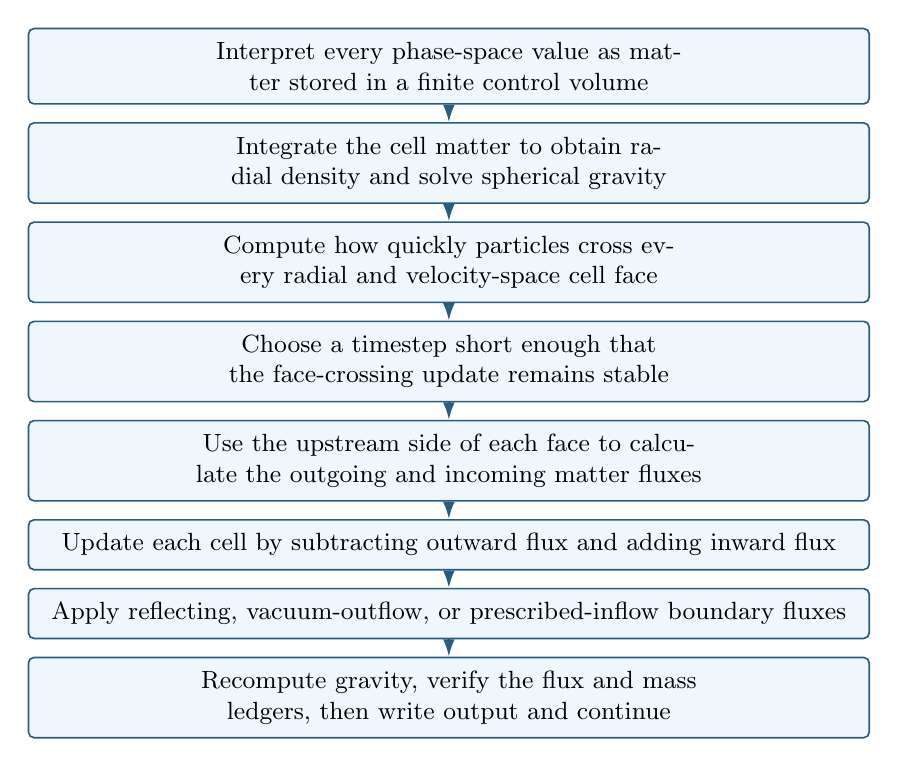
\begin{tikzpicture}[node distance=0.22cm]
\node[physicsflow] (fv1) {Interpret every phase-space value as matter stored in a finite control volume};
\node[physicsflow,below=of fv1] (fv2) {Integrate the cell matter to obtain radial density and solve spherical gravity};
\node[physicsflow,below=of fv2] (fv3) {Compute how quickly particles cross every radial and velocity-space cell face};
\node[physicsflow,below=of fv3] (fv4) {Choose a timestep short enough that the face-crossing update remains stable};
\node[physicsflow,below=of fv4] (fv5) {Use the upstream side of each face to calculate the outgoing and incoming matter fluxes};
\node[physicsflow,below=of fv5] (fv6) {Update each cell by subtracting outward flux and adding inward flux};
\node[physicsflow,below=of fv6] (fv7) {Apply reflecting, vacuum-outflow, or prescribed-inflow boundary fluxes};
\node[physicsflow,below=of fv7] (fv8) {Recompute gravity, verify the flux and mass ledgers, then write output and continue};
\draw[physicsarrow] (fv1) -- (fv2);
\draw[physicsarrow] (fv2) -- (fv3);
\draw[physicsarrow] (fv3) -- (fv4);
\draw[physicsarrow] (fv4) -- (fv5);
\draw[physicsarrow] (fv5) -- (fv6);
\draw[physicsarrow] (fv6) -- (fv7);
\draw[physicsarrow] (fv7) -- (fv8);
\end{tikzpicture}
\end{figure}

The semi-Lagrangian VP update follows characteristics. The finite-volume
option instead balances the matter entering and leaving each cell. Shared
face fluxes then give explicit local conservation, with the timestep limited
by the amount a donor cell can supply.  It computes face fluxes in \(r\) and
\(w\) using upwind states and subtracts the divergence from each control
volume:
\[
  f^{n+1}_{ijk}=f^n_{ijk}
  -\Delta t\left(\frac{F^r_{i+1/2,j,k}-F^r_{i-1/2,j,k}}{\Delta r_i}
  +\frac{F^w_{i,j+1/2,k}-F^w_{i,j-1/2,k}}{\Delta w_j}\right).
\]
The finite-volume implementation is in
\path{cpu/include/ev/vlasov_poisson.hpp}.  External inflow boundary conditions for
selected shell problems are built in the same file:
\codesource{\code{venus_cpu_vlasov_poisson_eulerian}}
  {\path{cpu/include/ev/vlasov_poisson.hpp}}
  {Shortened upwind finite-volume flux excerpt}
\begin{lstlisting}[language=C++]
const double flux_r = speed_r > 0.0 ? speed_r * f_left
                                    : speed_r * f_right;
const double flux_w = speed_w > 0.0 ? speed_w * f_down
                                    : speed_w * f_up;
f_new[q] = f[q] - dt * ((flux_r_hi - flux_r_lo) / dr
                      + (flux_w_hi - flux_w_lo) / dw);
\end{lstlisting}
At a fixed reflecting radial face \(R\), an outgoing velocity interval
\([w_-,w_+]\) maps to \([-w_+-2HR,-w_--2HR]\).  The finite-volume code
integrates \((w+HR)f\) over the outgoing part of each velocity cell and
distributes the opposite flux over the intersected incoming cells.  Summing
these two contributions cancels the radial mass flux to roundoff whenever
the reflected interval lies within the velocity domain.  Reflected velocities
outside that domain contribute to velocity-domain loss.  At an origin-parity
face \(R=0\), the same construction reverses \(w\).
The finite-volume timestep uses the sum of outgoing radial and velocity
flux coefficients divided by their cell widths.  At a reflecting face,
it uses the same velocity-cell integral as the wall flux.  This resolves a
wide velocity bin on a stretched grid even when its center lies near zero
radial speed.  Every positive donor cell enters this CFL limit, including
low-density tails, so its explicit outgoing contribution cannot exceed the
cell population within the configured Courant bound.


\noindent\textbf{Runnable starting point.}
The finite-volume branch uses the same VP physics selection but changes the
transport integrator.  A small \path{params.ini} is:
\codesource{\code{venus_cpu_vlasov_poisson_eulerian}}
  {\path{cpu/src/apps/vlasov_poisson/eulerian.cpp} and
   \path{cpu/include/ev/config.hpp}}
  {Example input for the explicit finite-volume VP branch}
\begin{lstlisting}[basicstyle=\ttfamily\scriptsize]
# params.ini: finite-volume Vlasov--Poisson run
physics_model = vlasov_poisson
vp_universe = static
vp_poisson_source = total_density
bp_collision_operator = none
kinetic_grid = legacy_nodal
initial_data = analytic
shell_initial_df = true
gaussian_density_shell = true
Nr = 96
Nw = 96
NL = 24
r_min = 1e-2
r_max = 40
w_max = 4
L_max = 6
integrator = conservative_finite_volume
inner_boundary = reflecting
outer_boundary = outflow_vacuum
t_end = 0.5
cfl = 0.35
dt_max = 0.01
output_dir = output/vp_finite_volume_example
\end{lstlisting}
Run it from the CPU source directory with:
\codesource{\code{venus_cpu_vlasov_poisson_eulerian}}
  {\path{cpu/Makefile} and \path{cpu/src/apps/vlasov_poisson/eulerian.cpp}}
  {Build and invocation commands}
\begin{lstlisting}[basicstyle=\ttfamily\scriptsize]
cd VENUS/cpu
make cpu-task-solvers
./venus_cpu_vlasov_poisson_eulerian --config params.ini
\end{lstlisting}

\subsection{Exact Finite-Angle Collision Foundations}

The marker modules begin with a two-body collision. Relative motion sets
the encounter rate, and conservation of momentum and energy determines the
outgoing velocities. This construction provides the basis for the collision
samplers and for the diffusion approximation introduced later.  Two incoming objects have
velocities \(\bm v_1,\bm v_2\), masses \(m_1,m_2>0\), relative velocity
\(\bm u=\bm v_1-\bm v_2\), and relative speed \(u=|\bm u|\).  A differential
cross section \(\dd\sigma/\dd\Omega\) gives the effective encounter area per
unit outgoing solid angle \(\dd\Omega\).  The local event rate is proportional
to
\[
  n_1 n_2\,u\,\frac{\dd\sigma}{\dd\Omega},
\]
where \(n_1,n_2\) are local number densities.  This factor explains the three
ingredients seen later in every exact sampler: find local partners, weight the
trial by relative speed and cross section, and draw an outgoing direction.

For an elastic event, the centre-of-mass velocity
\[
 \bm V=\frac{m_1\bm v_1+m_2\bm v_2}{m_1+m_2}
\]
is unchanged.  The outgoing relative velocity has the same length \(u\) but a
new direction \(\widehat{\bm n}\).  The unique outgoing velocities are
\[
 \bm v'_1=\bm V+\frac{m_2}{m_1+m_2}u\widehat{\bm n},
 \qquad
 \bm v'_2=\bm V-\frac{m_1}{m_1+m_2}u\widehat{\bm n}.
\]
These formulas conserve total momentum and kinetic energy for unequal as well
as equal masses.  Spherical variables are reconstructed only after this
three-dimensional collision has been completed.

\paragraph{Material SIDM.}
In a material self-interacting dark matter event, each marker represents
a sample of the continuous material distribution. The material law specifies
the cross section, often quoted per unit mass. Elastic scattering changes physical particle velocities while preserving
their rest masses. Each module specifies how numerical marker weights and
any unequal-weight remainder represent this event. Constant, power-law, and
Yukawa--Born laws have different dependences on \(u\) and scattering angle.
Their parameters therefore need the normalization and units of the selected
law.

\paragraph{Subhalo CDM encounters.}
In the subhalo operator, each marker represents one resolved extended
object.  The encounter area is derived from a softened Plummer gravitational
scattering model rather than a material cross section per mass.  An encounter
may scatter two complete subhaloes or, when the calibrated capture criterion
is met, replace them by one complete remnant.  The remnant has mass
\(m_1+m_2\), and the lost relative orbital energy is recorded as unresolved
internal energy.  This inelastic capture channel is not part of material
SIDM or the present SphDSMC module.

\paragraph{What the word exact means here.}
The pair kinematics above conserve the stated two-body invariants exactly.
The Monte Carlo sampler draws trial events from an upper rate, called a
majorant, and accepts each trial with the ratio of the physical rate to that
upper rate. A valid majorant makes this an unbiased sampling of the
represented discrete event process.  Numerical error still enters
through marker sampling, finite collision shells or cells, force resolution,
event cadence, rate bounds, finite run time, and random realization.  The
dense Eulerian operator described later uses the same word differently: it
enumerates every retained velocity-cell pair and configured angular node.
That label does not remove its angular quadrature, velocity boundary, remap,
or timestep error.

The Fokker--Planck operator appears only after these finite-angle constructions.
It represents the accumulated effect of many small deflections through
drift and diffusion coefficients. Its validity depends on the small-angle
regime, and its numerical accuracy requires convergence of those coefficients
and of the velocity space update.


\subsection{Eulerian Grid Collision Backends}
\label{sec:eulerian-grid-collisions}

\subsubsection{Scope, task executables, and operator names}

The modular CPU solver can add a radially local collision source to the
Vlasov--Poisson equation.  Here \(t\) is time, \(r\) is areal radius,
\(H(t)\) is the prescribed expansion rate, \(\Phi(t,r)\) is the Newtonian
gravitational potential, and a dot denotes differentiation along a particle
trajectory.  The symbol \(C[f]\) denotes the collision-induced rate of change
of the distribution \(f(t,r,w,L)\).  Its phase space variables are the
peculiar radial velocity \(w\), meaning radial velocity after subtracting
the expansion speed \(Hr\), and the specific angular momentum magnitude
\(L=rv_t\), where \(v_t\) is tangential-speed magnitude.  Cell-integrated
grids use the equivalent angular coordinate \(\eta=L^2/2\).  With these
definitions, the transport equation is
\[
 \frac{\partial f}{\partial t}
 +\dot r\,\frac{\partial f}{\partial r}
 +\dot w\,\frac{\partial f}{\partial w}
 =C[f],
 \qquad
 \dot r=Hr+w,\qquad
 \dot w=\frac{L^2}{r^3}-\Phi_r-Hw.                 \tag{EGC1}
\]
Here a subscript \(r\) means a radial derivative, so
\(\Phi_r=\partial\Phi/\partial r\).  The first term in
\(\dot w\) is the centrifugal acceleration, the second is gravity, and the
third removes the change in peculiar velocity caused by expansion.  At fixed
radius, the represented three-dimensional velocity-volume element is
\[
 \dd^3v=\frac{2\pi}{r^2}\,\dd w\,\dd\eta
       =\frac{2\pi}{r^2}L\,\dd w\,\dd L.            \tag{EGC2}
\]

\subsubsection{Cross-section conventions}

The Fokker--Planck (FP) and finite-angle operators represent different angular
limits of scattering.  Each kernel therefore uses the cross-section
convention derived below, even when the input parameter names coincide.

In the formulas below, \(u=|\boldsymbol v_1-\boldsymbol v_2|\) is the
relative speed of two particles.  The dimensionless factor
\(A=\code{bp_collision_strength}\) scales the collision rate;
\(\sigma_0\) is the configured reference area; \(u_0\) softens a power law
near zero speed; and \(n\) is its speed exponent.  For the Yukawa--Born law,
the numerical parameters \(\alpha_\chi,m_\chi,m_\phi\) set the amplitude
\(4\pi\alpha_\chi^2m_\chi^2/m_\phi^4\) and speed scale
\(m_\phi/m_\chi\).  The grid interprets the amplitude as an area in its
simulation units.  Material marker modules instead use area per mass, with
the physical conversion derived in Section~\ref{sec:yukawa-material-units}.
The total encounter area is
\(\sigma_{\rm tot}\).  The auxiliary areas \(\sigma_{\rm sat}\) and
\(\sigma_{\rm high}\), used by the softened-gravity law, are defined in
equation~(EGC4).

\paragraph{Total and differential finite-angle cross sections.}
The exact and reversible finite-angle branches use
\[
 \sigma_{\rm tot}(u)=
 \begin{cases}
 A\sigma_0,
   &\code{constant},\\
 A\sigma_0(u^2+u_0^2)^{-n/2},
   &\code{powerlaw},\\
 A\left(\sigma_{\rm sat}^{-1}+\sigma_{\rm high}^{-1}\right)^{-1},
   &\code{softened_gravity},\\
 \displaystyle
 A\frac{4\pi\alpha_\chi^2m_\chi^2}
 {m_\phi^4\left(1+m_\chi^2u^2/m_\phi^2\right)},
   &\code{yukawa_born}.
 \end{cases}                                             \tag{EGC5}
\]
The differential cross section \(\dd\sigma/\dd\Omega\) is encounter area per
unit outgoing solid angle \(\Omega\).  For an isotropic kernel, all outgoing
directions are equally likely:
\[
 \frac{\dd\sigma}{\dd\Omega}=\frac{\sigma_{\rm tot}}{4\pi}.
                                                               \tag{EGC6}
\]
Let \(\theta\) be the scattering deflection angle and
\(\mu=\cos\theta\).  For the Yukawa--Born kernel,
\[
 \frac{\dd\sigma}{\dd\Omega}
 =
 A\frac{\alpha_\chi^2m_\chi^2}
 {\left[m_\phi^2+\frac12m_\chi^2u^2(1-\mu)\right]^2},
 \qquad \mu=\cos\theta.                                  \tag{EGC7}
\]
With \path{bp_boltzmann_kernel=auto}, equation~(EGC7) is selected only for
\path{bp_cross_section=yukawa_born}; the other laws use isotropic scattering.
Notice that the Yukawa transfer cross section in equation~(EGC3) is not the
same object as the total and differential laws in equations~(EGC5)--(EGC7).

\subsubsection[Deterministic finite-angle quadrature]{
Deterministic finite-angle quadrature:
\code{boltzmann_exact}}

\paragraph{Meaning of ``exact''.}
The finite-angle continuum operator is
\[
 C[f](\boldsymbol v_1)=
 \int\dd^3v_2\int\dd\Omega\,
 u\frac{\dd\sigma}{\dd\Omega}
 \left[f(\boldsymbol v'_1)f(\boldsymbol v'_2)
       -f(\boldsymbol v_1)f(\boldsymbol v_2)\right].      \tag{EGC26}
\]
The vectors \(\boldsymbol v_1\) and \(\boldsymbol v_2\) are the two incoming
velocities, primes mark their outgoing values after a collision, and
\(\dd\Omega\) is an element of outgoing solid angle.  The gain term samples
states that scatter into \(\boldsymbol v_1\); the loss term samples particles
that scatter out of it.
The label \code{boltzmann_exact} refers to deterministic enumeration of every
retained Eulerian velocity-cell pair.  Angular quadrature, velocity boundaries,
time integration, and the outgoing remap still introduce discretization
errors.  The following derivation identifies each of these approximations.

At radial node \(i\), whose radius is \(r_i\), let \(a\) and \(b\) label the
two incoming velocity cells.  The angle \(\phi\) is their relative tangential
azimuth.  The unresolved incoming azimuth is represented by
\[
 \boldsymbol v_1=(w_a,L_a/r_i,0),\qquad
 \boldsymbol v_2=(w_b,(L_b/r_i)\cos\phi,
                  (L_b/r_i)\sin\phi).                    \tag{EGC27}
\]
The incoming \(\phi\) and outgoing azimuth \(\psi\) integrals use midpoint
rules.  The outgoing polar cosine is \(\mu=\cos\theta\), where \(\theta\) is
the deflection angle, and uses Gauss--Legendre quadrature.  The counts
\(N_{\phi,\rm pair}\), \(N_\mu\), and \(N_\psi\) are respectively the numbers
of incoming-azimuth, polar-cosine, and outgoing-azimuth nodes.  The parameter
consistency check requires at least
\[
 (N_{\phi,\rm pair},N_\mu,N_\psi)=(4,2,4),               \tag{EGC28}
\]
and defaults to \((4,4,4)\).

The occupation \(n_a\) of velocity cell \(a\) is
\[
 n_a=f_a\Delta^3v_a,\qquad
 \Delta^3v_a=\frac{2\pi}{r_i^2}\Delta w_a\,L_a\Delta L_a.
                                                               \tag{EGC29}
\]
For one unordered cell pair and angular node, define \(S_{ab}=1\) when
\(a\ne b\) and \(S_{aa}=1/2\), so a same-cell pair is not counted twice.
Let \(\omega_\mu\) be the Gauss--Legendre weight, let \(K(\mu;u)\) be the
selected angular kernel, and let \(\Delta t\) be the collision substep.  The
event occupation is
\[
 \Delta n=
 S_{ab}n_an_bu\sigma_{\rm tot}\Delta t\,
 \frac{1}{N_{\phi,\rm pair}}\,
 \frac{\omega_\mu K(\mu;u)}
      {\sum_{\mu'}\omega_{\mu'}K(\mu';u)}\,
 \frac{1}{N_\psi},                                      \tag{EGC30}
\]
The denominator normalizes the discrete polar probabilities to one.

Equal-mass centre-of-mass scattering gives
\[
 \boldsymbol V=\frac{\boldsymbol v_1+\boldsymbol v_2}{2},
 \qquad
 \boldsymbol v'_{1,2}=\boldsymbol V
 \pm\frac{u}{2}\widehat{\boldsymbol n}(\mu,\psi).         \tag{EGC31}
\]

\paragraph{Outgoing remap and boundaries.}
Each outgoing velocity is converted to
\[
 w'=v'_r,\qquad
 \eta'=\frac{r_i^2}{2}\left[(v'_\theta)^2+(v'_\phi)^2\right]
                                                               \tag{EGC32}
\]
and deposited bilinearly into at most four \((w,\eta)\) cells.  There is no
velocity reflection or extrapolation.  If either member of the outgoing pair
lies outside the stored \(w\) or \(L\) domain, the entire pair event is
omitted.  The code separately records \(w\)- and \(L\)-overflow activity and
aborts if the aggregate skipped fraction exceeds
\code{bp_boltzmann_remap_max_skipped_fraction}.

Cells below the configured distribution floor are inactive.
\code{bp_boltzmann_mass_tol}>0 removes the least populated active cells up to
that cumulative shell fraction; zero retains full represented support.

\paragraph{Time integration and repair.}
The operator is always explicit.  It estimates the largest loss frequency and
requires
\[
 \Delta t_{\rm coll}
 \le\frac{\code{bp_collision_cfl}}{\nu_{\max}}.           \tag{EGC33}
\]
It recomputes the loss bound and subcycles until the requested source interval
is consumed, aborting above \code{bp_collision_max_substeps}.

After clipping negative values, the optional
\code{bp_boltzmann_conserve_moments=true} repair adjusts each radial shell
toward its pre-collision mass, radial momentum, and kinetic energy:
\[
 f_q\leftarrow
 \max\!\left[
 0,\,
 f_q\{1+\alpha(\lambda_0+\lambda_1w_q+\lambda_2E_q)\}
 \right].                                                \tag{EGC34}
\]
Here \(q\) labels a velocity cell, \(E_q\) is its kinetic energy, and the
three multipliers \(\lambda_0,\lambda_1,\lambda_2\) are chosen to correct
mass, radial momentum, and kinetic energy.  The limiter \(\alpha\) keeps the
multiplicative correction positive.  A
singular \(3\times3\) repair system returns without a failure flag.  This
post-hoc repair does not establish detailed balance or a discrete
\(H\)-theorem.

The settings \code{bp_collision_flux},
\code{bp_collision_integrator}, \code{bp_sts_max_stages}, all bath and
coefficient-table controls, and \code{bp_collision_l_min_rel} are ignored by
\code{boltzmann_exact}.  In particular, Chang--Cooper and RKL2 must never be
listed as algorithms used by an exact finite-angle run merely because those
keys remain in its parameter file.

The dense cost scales approximately as
\[
 {\cal O}\!\left[
 N_rN_{\rm active}^2
 N_{\phi,\rm pair}N_\mu N_\psi
 \right].                                                \tag{EGC35}
\]
Radial shells are threaded dynamically; a sufficiently expensive shell also
uses pair-level parallelism with thread-private gain/loss arrays.

\subsubsection[Complete reversible finite-angle graph]{
Complete reversible finite-angle graph:
\code{boltzmann_reversible}}

This backend retains the finite-angle quadrature of
equations~(EGC26)--(EGC31) but replaces the independent outgoing remap with a
joint nonnegative pair projection.  It requires:
\codesource{Complete reversible-backend admissibility checks}{\path{cpu/include/ev/initial_data.hpp} and \path{cpu/include/ev/reversible_finite_angle_boltzmann.hpp}}{Requires a cell-integrated kinetic grid, conservative semi-Lagrangian transport, Strang splitting, zero mass pruning, and radial-velocity reflection closure}
\begin{lstlisting}
kinetic_grid = cell_average_eta
vp_interpolation = conservative_sldg
# or another cell-integrated SLDG option
bp_collision_splitting = strang
bp_boltzmann_mass_tol = 0
\end{lstlisting}
The radial-velocity grid must be closed under \(w\mapsto-w\).

For a velocity cell \(q\),
\[
 V_q=\frac{2\pi}{r_i^2}\Delta w_q\Delta\eta_q,\qquad
 E_q=\frac12\left(w_q^2+\frac{2\eta_q}{r_i^2}\right).     \tag{EGC36}
\]
For every outgoing continuous pair, the code searches an expanding candidate
stencil for nonnegative pair weights \(\alpha_m\) satisfying
\[
 \sum_m\alpha_m=1,                                       \tag{EGC37}
\]
\[
 \sum_m\alpha_m(w_{m1}+w_{m2})=w'_1+w'_2,                \tag{EGC38}
\]
\[
 \sum_m\alpha_m(E_{m1}+E_{m2})=E'_1+E'_2.                \tag{EGC39}
\]
The search begins at radius one and expands through
\code{bp_reversible_candidate_radius}.  A velocity outside the stored domain
is a domain omission; an in-domain pair for which no feasible nonnegative
hull is found is a projection omission.  Neither is reflected.

Each retained angular channel becomes a reversible reaction with coefficient
\[
 \kappa=
 \frac14V_aV_bu\sigma_{\rm tot}\,
 W_{\phi}W_\mu W_\psi.                                  \tag{EGC40}
\]
The factors \(W_\phi\), \(W_\mu\), and \(W_\psi\) are the normalized weights
of the incoming azimuth, outgoing polar cosine, and outgoing azimuth nodes.
Let \(\nu_q\) be its net population change and \(p_q\) its product exponent.
The reaction flux is
\[
 J=\kappa\left(f_af_b-\prod_q f_q^{p_q}\right),\qquad
 \frac{\dd f_q}{\dd t}=\frac{\nu_q}{V_q}J.               \tag{EGC41}
\]
This is implemented through logarithms:
\codesource{Complete reversible reaction flux}{\path{cpu/include/ev/reversible_finite_angle_boltzmann.hpp}}{Evaluates forward and reverse activities in a positivity-aware logarithmic form and accumulates each species population change conservatively}
\begin{lstlisting}[language=C++]
forward = f[incoming_first] * f[incoming_second];
log_reverse += species.product_order * log(f[species.index]);
reverse = exp(log_reverse);
flux = reaction.coefficient * (forward - reverse);
rhs[q] += species.net_population_change * flux / volume[q];
\end{lstlisting}

Equations~(EGC37)--(EGC39) imply reaction-level number, radial-momentum, and
kinetic-energy conservation.  A discrete drifting Maxwellian has
\[
 \log f_q=a+bw_q-cE_q,                                   \tag{EGC42}
\]
so the same constraints make its forward and reverse activities identical.
For
\[
 H_h=\sum_qV_qf_q(\log f_q-1),                           \tag{EGC43}
\]
\(H_h\) is the discrete Boltzmann \(H\)-functional: \(V_q\) is the
velocity-cell volume and \(f_q\) its nonnegative distribution value.  A
discrete \(H\)-theorem is the statement that this quantity cannot increase
under the collision update.  Physical entropy has the opposite sign.
For the continuous-time evolution of the discrete populations, each reaction
contributes a term proportional to
\[
 (x-y)\log(y/x)\le0,\qquad
 x=f_af_b,\quad y=\prod_qf_q^{p_q}.                      \tag{EGC44}
\]
Thus every represented reaction conserves the three collision invariants,
has the discrete Maxwellian null space, and dissipates \(H_h\).

\paragraph{Positive finite-time reaction extent.}
A scalar extent moves all participating cells together:
\[
 f_q(\xi)=f_q(0)+\frac{\nu_q}{V_q}\xi.                   \tag{EGC45}
\]
Positivity restricts it to
\[
 \max_{\nu_q>0}\left(-\frac{f_qV_q}{\nu_q}\right)
 \le\xi\le
 \min_{\nu_q<0}\left(-\frac{f_qV_q}{\nu_q}\right).       \tag{EGC46}
\]
If Euler and Heun extents remain strictly inside this interval and do not
reverse the flux sign, VENUS accepts the second-order Heun extent.  Otherwise
it solves
\[
 \xi-\Delta t\,J[f(\xi)]=0                              \tag{EGC47}
\]
with safeguarded Newton iterations inside a bisection bracket.  One collision
source step applies every reaction for half a step in forward graph order and
then for half a step in reverse order.  The final state is checked for
nonnegativity and nonincrease of equation~(EGC43).

When \code{bp_reversible_explicit_fast_path=true} and the full interval
satisfies the initial positivity limit, the code first tries its reference
SSPRK2 update.  A failed second-stage positivity or entropy check falls back
to the symmetric reaction-extent sweep.  This logic is independent of
\code{bp_collision_integrator}; the FP \code{explicit}/\code{sts_rkl2}
selection does not control a reversible graph.

\paragraph{Omission guard and cost.}
The code checks both the volume-integrated omitted activity and every
physically active shell.  A run fails if either exceeds
\code{bp_boltzmann_remap_max_skipped_fraction}.  Very low-activity shells are
classified using \code{bp_reversible_active_shell_floor_fraction}.

The complete graph scales as
\[
 {\cal O}\!\left[(N_wN_L)^2
 N_{\phi,\rm pair}N_\mu N_\psi\right]                   \tag{EGC48}
\]
per radial shell.  \code{bp_reversible_max_velocity_cells} is an explicit
memory/runtime guard for this complete-graph oracle.  It does not constrain
the sampled or streamed variants.  Likewise,
\code{bp_boltzmann_conserve_moments} is irrelevant here: represented
reversible reactions conserve the moments intrinsically.

\subsubsection[Hybrid sampled reversible graph]{
Hybrid sampled reversible graph:
\code{boltzmann_reversible_sampled}}

This backend evaluates a time-reversal-closed dense subset exactly and
importance-samples its complement.  Every sampled channel is still converted
to the same invariant-preserving reversible reaction described by
equations~(EGC37)--(EGC47).

\paragraph{Current full-support proposal.}
Let \(M=N_wN_L\), \(V_q\) be equation~(EGC36), and
\(n_q=V_qf_q\).  The implemented one-cell distributions are
\[
 p_q^{\rm bulk}\propto n_q,\qquad
 p_q^{\rm phase}\propto f_q,                             \tag{EGC49}
\]
\[
 p_q^{\rm tail}\propto
 n_q\left(1+\frac{E_q}{\langle E\rangle}\right)^{p_{\rm tail}},
                                                               \tag{EGC50}
\]
and
\[
 p_q^{\rm eq}\propto
 V_q\exp(\beta w_q-\gamma E_q),\qquad
 \beta=\frac{\langle w\rangle}{T},\quad
 \gamma=\frac1T,\quad
 T=\frac23\left(\langle E\rangle-\frac{\langle w\rangle^2}{2}\right).
                                                               \tag{EGC51}
\]
The exponent \(p_{\rm tail}=\code{bp_sampled_tail_power}\) biases the tail
proposal toward high-energy cells.  Each \(\lambda_*\) below is a
nonnegative mixture fraction for the named proposal component; all six
fractions, including the derived \(\lambda_{\rm bulk}\), sum to one.
The stratified component groups cells by energy rank, sign of \(w\), and
angular momentum bin.  Stratum pairs and incoming azimuths are further binned
by representative relative speed and weighted by an activity proxy.

The exact current mixture is
\begin{equation}
\tag{EGC52}
\begin{split}
 q(a,b,\phi)={}&
 \lambda_{\rm bulk}\,
 p_a^{\rm bulk}p_b^{\rm bulk}\frac1{N_\phi}
 +\lambda_{\rm tail}\,
 p_a^{\rm tail}p_b^{\rm tail}\frac1{N_\phi}\\
 &+\lambda_{\rm eq}\,
 p_a^{\rm eq}p_b^{\rm eq}\frac1{N_\phi}
 +\lambda_{\rm phase}\,
 p_a^{\rm phase}p_b^{\rm phase}\frac1{N_\phi}\\
 &+\lambda_{\rm strat}q_{\rm strat}(a,b,\phi)
 +\lambda_{\rm unif}\frac1{M^2N_\phi}.
\end{split}
\end{equation}
where
\[
 \lambda_{\rm bulk}
 =
 1-\lambda_{\rm tail}-\lambda_{\rm eq}
  -\lambda_{\rm phase}-\lambda_{\rm strat}
  -\lambda_{\rm unif}.                                  \tag{EGC53}
\]
A strictly positive \(\lambda_{\rm unif}\) is required so every represented
pair and azimuth has nonzero probability.

The dense cells are ranked by an activity proxy and selected together with
their radial reversals
\[
 (j,k)\longmapsto(N_w-1-j,k).                            \tag{EGC54}
\]
Consequently the exact dense block and its sampled complement are both closed
under \(w\mapsto-w\).

\paragraph{Complement importance weight.}
Let \(Z_C\) be the total probability of lying outside the dense block and let
\(N\) be the samples per batch.  For a complement state
\(x=(a,b,\phi)\), a non-antithetic channel has coefficient
\[
 \kappa_s=
 \frac14V_aV_bu\sigma_{\rm tot}
 \frac{Z_C}
 {N\,N_\phi\,q(x)\,K_\Omega},                            \tag{EGC55}
\]
where \(K_\Omega=\code{bp_sampled_outgoing_angle_samples}\).
When the radial reverse \(\bar x\) also lies in the complement, both members
are inserted with the paired weight
\[
 \kappa_s=
 \frac14V_aV_bu\sigma_{\rm tot}
 \frac{Z_C}
 {N\,N_\phi\,[q(x)+q(\bar x)]\,K_\Omega}.                \tag{EGC56}
\]
This antithetic construction improves coverage of the odd radial component
that transports heat.

The actual operator samples the configured discrete angular quadrature:
Gauss--Legendre \(\mu\) nodes weighted by the selected differential kernel and
midpoint \(\psi\) nodes.  It does not use the continuous inverse-Yukawa
utility retained for analytic kernel calculations.

With \code{bp_sampled_ntc_pair_thinning=true}, a pilot quantile sets a
threshold in \(u\sigma\).  A retained low-activity pair receives the inverse
acceptance probability, preserving the expectation.  If the requested
batch-accuracy tolerance is not met at the cap, the sampled implementation
disables thinning, rebuilds from the starting sample count, and tries once
more before applying \code{bp_sampled_fail_on_unconverged}.

\paragraph{Independent-replicate error estimate.}
If \(R=\code{bp_sampled_replicates_per_estimate}\), this backend constructs two
independently shifted families for each requested replicate: the total number
of batch estimates is \(R_{\rm tot}=2R\).  For batch collision fields
\(Q^{(s)}\),
\[
 \overline Q=\frac1{R_{\rm tot}}\sum_sQ^{(s)},\qquad
 S_Q^2=
 \frac1{R_{\rm tot}(R_{\rm tot}-1)}
 \sum_s\|Q^{(s)}-\overline Q\|_V^2.                      \tag{EGC57}
\]
The velocity-volume norm is
\(\|X\|_V=[\sum_qV_qX_q^2]^{1/2}\); it weights each cell by the physical
velocity volume in equation~(EGC36).
The accepted normalized error is
\[
 \epsilon_Q=
 \frac{S_Q}
 {\max\{\|\overline Q\|_V,\,
 \lambda_Q\|\overline G\|_V,\,10^{-300}\}},              \tag{EGC58}
\]
where \(G\) is the nonnegative forward-plus-reverse traffic and
\(\lambda_Q=\code{bp_sampled_rhs_floor_fraction}\).

The conductive diagnostic for batch \(s\) is
\[
 h^{(s)}=\sum_qV_qE_qw_qQ_q^{(s)}.                       \tag{EGC59}
\]
Its standard error is normalized by the larger of
\(|\overline h|\) and
\code{bp_sampled_heat_floor_fraction} times the gross absolute heat traffic.
Samples per batch double until both RHS and heat criteria pass or the
configured maximum is reached.  A low-discrepancy sequence is a deterministic
point set designed to fill the unit sampling cube more evenly than unrelated
random draws.  VENUS uses shifted Halton coordinates: radical-inverse
sequences in distinct prime bases receive an independent random shift for
each replicate.  Existing low-discrepancy ranges are retained when a batch is
enlarged.

The final graph is the arithmetic mean of all \(2R\) sampled graphs plus the
single deterministic dense graph.  This backend does not persist or reuse an
operator graph between collision calls; graph-reuse controls belong only to
the streamed implementation.

\paragraph{Shell planning and locality.}
For each shell the code estimates
\[
 \lambda_{\rm rms}=
 \frac{1}{n\,\sigma_{\rm tot}(u_{\rm rms})},\qquad
 \chi_{\rm loc}=\frac{\Delta r}{\lambda_{\rm rms}}.       \tag{EGC60}
\]
Here \(n=\sum_qV_qf_q\) is the shell number density and
\(u_{\rm rms}=[2(\langle v^2\rangle-\langle w\rangle^2)]^{1/2}\) is the
root-mean-square relative-speed estimate used only for this locality check.
If \(\chi_{\rm loc}>\code{bp_collision_locality_max_ratio}\) and
\code{bp_collision_fail_on_nonlocal_cells=true}, the run aborts and requests
radial refinement.

The starting batch count is raised by powers of two according to
\[
 {\cal A}_i=n_i^2\langle v\rangle_i
 \sigma_{\rm tot}(\langle v\rangle_i),\qquad
 N_i\propto({\cal A}_i/{\rm median}\,{\cal A})^{1/4},     \tag{EGC61}
\]
capped by \code{bp_sampled_activity_boost_max}.  Rigorously bounded
low-activity shells may be made inactive only while their accumulated upper
bound fits within one tenth of the global omission budget.

\subsubsection[Streamed reversible graph]{
Streamed reversible graph:
\code{boltzmann_reversible_streamed}}

The streamed backend uses the same physical kernel, proposal mixture,
time-reversal pairing, joint projection, reaction flux, positivity bounds,
invariants, entropy functional, omission budget, and locality criterion as the
sampled backend.  Its different implementation is designed to reduce the
large temporary graph and projection cost.

It is not graph-free.  It:
\begin{enumerate}
\item builds and caches the exact time-reversal-closed dense graph;
\item samples the conditional complement with shifted Halton coordinates;
\item optionally performs a guided pilot and mixes its ranked-pair proposal
      with the full-support base proposal;
\item accumulates RHS, gross traffic, omitted activity, and hashed reaction
      coefficients without immediately constructing duplicate reaction
      objects;
\item combines repeated sampled channels into a compact reaction graph;
\item applies the same positive symmetric reaction-extent integrator as the
      complete and sampled reversible backends.
\end{enumerate}

For canonical reversal orbit \(x,\bar x\), define
\[
 p_{\rm base}(x)=\frac{q(x)+q(\bar x)}{Z_C},\qquad
 p_{\rm samp}(x)=(1-g)p_{\rm base}(x)+g\,p_{\rm guide}(x),
                                                               \tag{EGC62}
\]
where \(g=\code{bp_sampled_guided_fraction}\).
Before final averaging, one sampled pair carries
\[
 \widetilde\kappa_s=
 \frac14V_aV_bu\sigma_{\rm tot}
 \frac{1}{N_\phi p_{\rm samp}(x)}
 \frac{1}{P_{\rm NTC}}\,
 P_\Omega.                                               \tag{EGC63}
\]
Here \(P_{\rm NTC}=u\sigma/(u\sigma)_{\max}\) for retained thinned events and
one otherwise; \(P_\Omega\) is the selected discrete angular probability.
The materialized coefficient is divided by the number of production batches
and samples per batch.

If
\[
 K_\Omega=N_\mu N_\psi,                                  \tag{EGC64}
\]
the streamed branch visits the complete configured angular tensor product.
Otherwise it makes \(K_\Omega\) stratified draws from the same discrete
Gauss--Legendre/midpoint angular rule.

A separate two-batch controller demands one quarter of the requested RHS and
heat tolerances before choosing the production count.  The production stage
uses
\[
 N_{\rm prod}=\max(2,\code{bp_sampled_replicates_per_estimate})
                                                               \tag{EGC65}
\]
independent batches, evaluates equation~(EGC57), and doubles the count if
necessary.  This differs from the sampled backend's \(2R\) semantics.

\paragraph{Persistent workspace and graph refresh.}
The streamed workspace contains a projection cache, dense-graph cache, and
per-shell operator-graph cache.  With
\path{bp_sampled_fixed_geometric_sequence=true}, the low-discrepancy geometry
is determined only by the user seed and shell identifier; false additionally
hashes the current shell distribution.

With \code{bp_sampled_reuse_operator_graph=true}, an existing graph may be
reused while
\[
 \delta_1=
 \frac{\sum_qV_q|f_q-f_q^{\rm ref}|}
 {\max\{\sum_qV_qf_q,\sum_qV_qf_q^{\rm ref}\}}
 \le
 \code{bp_sampled_operator_refresh_l1_fraction}.         \tag{EGC66}
\]
A changed grid, projection stencil, angular rule, cross section, kernel,
softened-gravity data (\(G\), subhalo mass/radius, or Coulomb logarithm),
reversible entropy floor, unconverged-estimate policy, or sampling
configuration invalidates the workspace.  Projection records are retained up
to the implementation cap and then discarded shell by shell.  Reusing a
cached graph also reuses its recorded convergence state; it is never relabeled
as converged merely because the graph was already resident.

This workspace is memory-resident rather than restart-serialized.  A restarted
run rebuilds it.  When graph reuse is enabled, an uninterrupted run may
therefore follow a different sampled numerical trajectory from a restarted
run because the uninterrupted run can reuse an older admissible graph while
the restarted run constructs a new graph from the checkpoint DF.

The three controls
\codesource{Streamed reversible operator-graph workspace}{\path{cpu/include/ev/config.hpp} and \path{cpu/include/ev/streamed_reversible_boltzmann.hpp}}{Controls geometry seeding, persistent graph reuse, and the distribution-change threshold that forces graph reconstruction}
\begin{lstlisting}
bp_sampled_fixed_geometric_sequence
bp_sampled_reuse_operator_graph
bp_sampled_operator_refresh_l1_fraction
\end{lstlisting}
apply only to \code{boltzmann_reversible_streamed}.  They are wired through
the INI and CLI parsers, consistency checks, and metadata together with the
persistent standard-solver workspace.

\subsubsection{Small-angle approximation: Fokker--Planck/Landau}

The finite-angle law above is the governing collision physics.  The
Fokker--Planck branch replaces many individually small deflections by a
continuous drift and diffusion in velocity space.  It is useful only
when that accumulated-small-angle picture is resolved and physically
appropriate.  The next reference block states exactly which continuum
coefficients and discrete fluxes VENUS uses.

\paragraph{FP transfer cross section.}
Writing \(A=\code{bp_collision_strength}\), the FP coefficient integrals use
the effective momentum-transfer cross section
\[
 \sigma_T(u)=
 \begin{cases}
 A\sigma_0,&\code{constant},\\[1mm]
 A\sigma_0(u^2+u_0^2)^{-n/2},&\code{powerlaw},\\[1mm]
 A(\sigma_{\rm sat}^{-1}+\sigma_{\rm high}^{-1})^{-1},
   &\code{softened_gravity},\\[1mm]
 \displaystyle A\frac{8\pi\alpha_\chi^2}{m_\chi^2u^4}
 \left[\ln(1+x)-\frac{x}{1+x}\right],\quad
 x=\frac{m_\chi^2u^2}{m_\phi^2},&\code{yukawa_born}.
 \end{cases}                                             \tag{EGC3}
\]
Here
\[
 \sigma_{\rm sat}=\begin{cases}\sigma_0,&\sigma_0>0,\\
 2\pi\epsilon^2,&\sigma_0=0,\end{cases}\qquad
 \sigma_{\rm high}=\frac{4\pi G^2m_{\rm sub}^2\ln\Lambda}{u^4}. \tag{EGC4}
\]
The symbols \(\epsilon\), \(G\), \(m_{\rm sub}\), and \(\ln\Lambda\)
are the softening length, Newtonian gravitational constant, represented
subhalo mass, and Coulomb logarithm.  The transfer cross section weights each
deflection by its momentum transfer; it is an angular moment of the
differential law, not the finite-angle total encounter area.  The
softened-gravity plateau is a physical geometrical area, not a generic
material cross section per mass.


\paragraph{Continuum approximation.}
The labels \code{fokker_planck} and \code{landau_fp} advance
\[
 C_{\rm FP}[f]
 =-\frac{\partial}{\partial v_i}(D_i f)
  +\frac12\frac{\partial^2}{\partial v_i\partial v_j}
                  (D_{ij}f).                             \tag{EGC8}
\]
Cartesian velocity components are indexed by \(i,j\in\{1,2,3\}\), with
repeated indices summed.  The vector \(D_i\) is the velocity space drift and
the symmetric tensor \(D_{ij}\) is the velocity space diffusion.
For relative velocity
\(\boldsymbol u=\boldsymbol v-\boldsymbol v_\star\), the implemented
small-angle coefficients are
\[
 D_i=-\frac12\int\dd^3v_\star\,
 f_\star\,u\,\sigma_T(u)\,u_i,                            \tag{EGC9}
\]
\[
 D_{ij}=\frac14\int\dd^3v_\star\,
 f_\star\,u^3\sigma_T(u)
 \left(\delta_{ij}-\frac{u_i u_j}{u^2}\right).            \tag{EGC10}
\]
Here \(\boldsymbol v\) is the velocity at which a coefficient is evaluated,
\(\boldsymbol v_\star\) is a bath-particle velocity,
\(f_\star=f(\boldsymbol v_\star)\), and \(\delta_{ij}\) is one for \(i=j\)
and zero otherwise.  The projector in parentheses removes diffusion along
the relative-velocity direction.
These expressions explain why this branch requires a transfer cross section,
whereas finite-angle scattering requires a differential kernel.

\paragraph{Bath choices.}
The coefficient source is controlled by \code{bp_bath}.
\begin{description}
\item[\code{instantaneous_df}] Equation~(EGC9)--(EGC10) is quadrature-summed
      directly over the current local Eulerian DF.  Low-population partner
      cells may be removed with \code{bp_partner_mass_tol}; zero retains the
      complete represented support.  The expensive coefficients are evaluated
      on a reduced \((w,L)\) table and interpolated onto the full grid.
\item[\code{local_maxwellian}] Each radial shell is replaced, for coefficient
      construction only, by
      \[
       f_\star(s)=\frac{\rho}
       {(2\pi\Theta)^{3/2}}\exp[-s^2/(2\Theta)].           \tag{EGC11}
      \]
      VENUS obtains
      \[
       \rho=\frac{2\pi}{r^2}\int fL\,\dd w\,\dd L,\qquad
       U=\langle w\rangle,\qquad
       \Theta=\frac{\langle(w-U)^2\rangle+\langle v_t^2\rangle}{3},
                                                               \tag{EGC12}
      \]
      subject to the configured density and temperature floors.
\item[\code{global_maxwellian}] Shell density is volume-averaged, bulk velocity
      is mass-weighted, and the global temperature uses the full second moment,
      including shell-to-shell radial streaming.
\end{description}

The Maxwellian integral uses midpoint quadrature in bath speed and polar
cosine up to
\(\code{bp_bath_speed_cutoff}\sqrt{\Theta}\).  It is tabulated versus evaluation
speed with \code{bp_coeff_table_points} entries and cubic interpolation.
\code{bp_coeff_speed_points} and \code{bp_coeff_mu_points} control its
quadrature.

\paragraph{Projection onto \((w,L)\) and \((w,\eta)\).}
Let
\[
 c_r=w-U,\qquad c_t=L/r,\qquad
 V=(c_r^2+c_t^2)^{1/2},\qquad e_r=c_r/V,\quad e_t=c_t/V.
\]
If \(A_\parallel\) is the drift amplitude along the local relative-velocity
direction, and \(D_\parallel\) and \(D_\perp\) are the parallel and transverse
diffusion coefficients obtained from equations~(EGC9)--(EGC10), VENUS
constructs
\[
 D_r=A_\parallel e_r,\qquad
 D_L=rA_\parallel e_t,                                   \tag{EGC13}
\]
\[
 D_{rr}=D_\perp+(D_\parallel-D_\perp)e_r^2,
\]
\[
 D_{rL}=r(D_\parallel-D_\perp)e_re_t,
\]
\[
 D_{LL}=r^2[D_\perp+(D_\parallel-D_\perp)e_t^2],
 \qquad D_{aa}=r^2D_\perp.                               \tag{EGC14}
\]
Changing variables to \(\eta=L^2/2\) gives
\[
 D_w=D_r,\qquad
 D_\eta=LD_L+\frac12(D_{LL}+D_{aa}),                     \tag{EGC15}
\]
\[
 D_{ww}=D_{rr},\qquad
 D_{w\eta}=LD_{rL},\qquad
 D_{\eta\eta}=L^2D_{LL}.                                 \tag{EGC16}
\]
The \(D_{aa}\) term is the It\^o/geometrical contribution from rotations out
of the selected tangential plane: the index \(a\) denotes the unresolved
tangential-azimuth direction orthogonal to the stored radial--\(L\) plane,
not a grid-cell label.  The source implementation is:
\codesource{Fokker--Planck coefficient map to \(w,\eta\)}{\path{cpu/include/ev/boltzmann_poisson.hpp}}{Transforms radial and tangential drift--diffusion coefficients into the solver's radial-velocity and squared-angular momentum variables}
\begin{lstlisting}[language=C++]
out.D_w      = c.D_r;
out.D_eta    = L * c.D_L + 0.5 * (c.D_LL + c.D_aa);
out.D_ww     = c.D_rr;
out.D_weta   = L * c.D_rL;
out.D_etaeta = L * L * c.D_LL;
\end{lstlisting}

\paragraph{Finite-volume flux.}
The conservative update is
\[
 \partial_t f=-\partial_wF_w-\partial_\eta F_\eta,        \tag{EGC17}
\]
with
\[
 F_w=D_wf-\frac12\partial_w(D_{ww}f)
             -\frac12\partial_\eta(D_{w\eta}f),           \tag{EGC18}
\]
\[
 F_\eta=D_\eta f-\frac12\partial_\eta(D_{\eta\eta}f)
             -\frac12\partial_w(D_{w\eta}f).              \tag{EGC19}
\]
For a diagonal face, put \(K=D_{xx}/2\),
\(\mathrm{Pe}=A_x\Delta x/K_{\rm face}\), and
\(\mathcal B(z)=z/(\exp z-1)\).  The Chang--Cooper/exponential-fit flux is
\[
 F_{i+1/2}
 =
 \frac{
  \mathcal B(-\mathrm{Pe})K_i f_i
  -\mathcal B(\mathrm{Pe})K_{i+1}f_{i+1}}
 {\Delta x}.                                             \tag{EGC20}
\]
The dimensionless P\'eclet number \(\mathrm{Pe}\) compares drift transport
\(A_x\Delta x\) with face diffusion \(K_{\rm face}\); its sign follows the
drift direction.
Despite the input name \code{centered}, that alternative uses upwind drift
and centered diffusion; it is not centered advection.

The outer \(w\) faces, upper \(\eta\) face, and lower active-\(L\) face have
zero collision flux.  The optional
\code{bp_collision_l_min_rel} moves the lower active-\(L\) face upward and
therefore deliberately removes collision coupling below that cutoff.

\paragraph{Explicit and RKL2 integration.}
The explicit stability estimate includes
\[
 \frac{D_{ww}}{\Delta w^2},\qquad
 \frac{D_{\eta\eta}}{\Delta\eta^2},\qquad
 \frac{|D_{w\eta}|}{\Delta w\,\Delta\eta},                \tag{EGC21}
\]
and, for the \code{centered} branch, the drift rates
\(|D_w|/\Delta w\) and \(|D_\eta|/\Delta\eta\).
The explicit branch uses
\[
 N_{\rm sub}=\left\lceil
 \frac{\Delta t}{\Delta t_{\rm stable}}\right\rceil       \tag{EGC22}
\]
and aborts if this exceeds \code{bp_collision_max_substeps}.

With \code{bp_collision_integrator=sts_rkl2}, a cycle with \(s\) stages has
the nominal acceleration
\[
 a_s=\frac{s^2+s-2}{4}.                                  \tag{EGC23}
\]
The implementation chooses the smallest sufficient stage count, capped by
\code{bp_sts_max_stages}, and uses multiple cycles if one capped cycle cannot
cover the source interval.

The stages approximate the frozen-coefficient flux equation
\(\partial_t f={\cal L}_h f\), where \({\cal L}_h\) is the discrete
operator in (EGC17)--(EGC20).  Its coefficients stay fixed during one
cycle of duration \(\Delta t\).  The second-order Runge--Kutta--Legendre
construction of
\href{https://doi.org/10.1016/j.jcp.2013.08.021}{Meyer, Balsara, and Aslam (2014)}
uses
\[
 w_1=\frac{4}{s^2+s-2},\qquad b_0=b_1=\frac13,\qquad
 b_j=\frac{j^2+j-2}{2j(j+1)}\quad(2\le j\le s).
                                                        \tag{EGC23a}
\]
Here \(j\) counts internal stages within one physical timestep, and
\(s\ge2\) is the total number of stages.  Set
\[
 \mu_j=\frac{2j-1}{j}\frac{b_j}{b_{j-1}},\quad
 \nu_j=-\frac{j-1}{j}\frac{b_j}{b_{j-2}},\quad
 \widetilde\mu_j=\mu_jw_1,\quad
 \widetilde\gamma_j=-(1-b_{j-1})\widetilde\mu_j.
                                                        \tag{EGC23b}
\]
Starting from \(Y_0=f^n\), the recurrence for \(2\le j\le s\) is
\begin{align}
 Y_1&=Y_0+b_1w_1\Delta t\,{\cal L}_hY_0,\notag\\
 Y_j&=\mu_jY_{j-1}+\nu_jY_{j-2}+(1-\mu_j-\nu_j)Y_0\notag\\
 &\quad+\widetilde\mu_j\Delta t\,{\cal L}_hY_{j-1}
 +\widetilde\gamma_j\Delta t\,{\cal L}_hY_0,
 \qquad f^{n+1}=Y_s.                                   \tag{EGC23c}
\end{align}
The first-stage factor is \(b_1w_1=w_1/3\); subsequent source terms use
\(\mu_jw_1\).  Expanding this recurrence gives
\(Y_s=f^n+\Delta t{\cal L}_hf^n+
\Delta t^2{\cal L}_h^2f^n/2+O(\Delta t^3)\), which states its
second-order consistency for the frozen linear operator.
\codesource{RKL2 frozen-coefficient stage update}
{\path{cpu/include/ev/boltzmann_poisson.hpp}}
{Combines the two preceding stages and the initial and current flux right-hand sides}
\begin{lstlisting}[language=C++,basicstyle=\ttfamily\scriptsize]
yj[s] = mu * ym1[s] + nu * ym2[s]
    + (1.0 - mu - nu) * y0[s]
    + mu_tilde * dt * rhsm1[s]
    + gamma_tilde * dt * rhs0[s];
\end{lstlisting}
The C++ index \code{s} in this excerpt is a flattened phase space array
offset; the enclosing loop variable \code{j} selects the stage.
A finite decay-mode validation evolves an exact decay
mode of the same discrete flux and checks temporal consistency and
second-order refinement at two, three, and eight stages.

After every explicit substep or RKL2 cycle, negative cells are clipped.  If
the shell has positive mass \(P\) and clipped negative mass \(N\), every
positive cell is multiplied by
\[
 \max(0,(P-N)/P).                                        \tag{EGC24}
\]
This preserves shell mass when \(P\ge N\), but it does not repair radial
momentum or kinetic energy.  The FP discretization therefore has conservative
number fluxes but no discrete momentum, energy, or \(H\)-theorem guarantee
comparable to the reversible operator.

\paragraph{Coefficient refresh and tracers.}
Coefficient tables can be refreshed every
\path{bp_coeff_refresh_every} source applications or after
\[
 \Delta t_{\rm refresh}
 =\code{bp_coeff_refresh_chi}\,t_{\rm coll},              \tag{EGC25}
\]
where \(t_{\rm coll}\) is the configured mass-weighted collision-time
quantile.  A tracer is advanced by the same frozen linear operator; it does
not contribute to the bath.  Here a \emph{passive tracer} is a second
distribution used to follow a tagged population without allowing that
population to alter the FP coefficient bath.

The cadence and coefficient caches live in process memory and are not written
to a restart.  For restart-equivalent numerical scheduling, use
\code{bp_collision_apply_every=1}, or the paired multirate Strang macro-step
described below.  A fresh process otherwise rebuilds the coefficients and
resets a partially accumulated non-Strang cadence.

\paragraph{Diagnostic term masks.}
\code{bp_fp_terms} accepts
\code{full}, \code{vr_only}, \code{L_only}, \code{no_mixed},
\code{no_azimuth}, \code{no_drift}, \code{drift_only}, \code{Drr_only},
\code{DLL_only}, and \code{Daa_only}.  Values other than \code{full} are
diagnostic operator mutilations and need not retain the conservation or
equilibrium properties of the complete tensor.

\subsubsection{Selecting a backend and process layout}

Only after choosing the physical operator above should one select its
implementation label.  The accepted values are
\codesource{Eulerian collision-operator selection}{\path{cpu/include/ev/config.hpp} and \path{cpu/include/ev/initial_data.hpp}}{Parses the operator label and rejects every value outside the implemented Fokker--Planck, exact, and reversible backend set}
\begin{lstlisting}
bp_collision_operator = fokker_planck
bp_collision_operator = landau_fp
bp_collision_operator = boltzmann_exact
bp_collision_operator = boltzmann_reversible
bp_collision_operator = boltzmann_reversible_sampled
bp_collision_operator = boltzmann_reversible_streamed
\end{lstlisting}
The two FP names select the same coefficient formula.  The names
\code{boltzmann_exact_sampled} and \code{boltzmann_exact_streamed} are not
valid values.

Each operator also has a task-specific frontend:
\codesource{Fail-closed Eulerian collision task fronts}{\path{cpu/Makefile} and \path{cpu/include/ev/solver_task_profile.hpp}}{Registers each executable name and locks it to the matching Boltzmann--Poisson operator before state or output construction}
\begin{lstlisting}[basicstyle=\ttfamily\scriptsize]
venus_cpu_boltzmann_poisson_fokker_planck
venus_cpu_boltzmann_poisson_landau
venus_cpu_boltzmann_poisson_exact
venus_cpu_boltzmann_poisson_reversible
venus_cpu_boltzmann_poisson_reversible_sampled
venus_cpu_boltzmann_poisson_reversible_streamed
venus_cpu_boltzmann_poisson_expanding_prompt_cusp
\end{lstlisting}
These backends use one Message Passing Interface (MPI) rank and parallelize
within it with OpenMP or the standard-thread fallback; collision fluxes and
reaction data are not exchanged between MPI angular momentum slabs.  The FP
branch can advance the passive tracer defined above, whereas all four
finite-angle branches reject a nonempty tracer.  The implementations live in
\path{cpu/include/ev/boltzmann_poisson.hpp},
\path{cpu/include/ev/finite_angle_boltzmann.hpp},
\path{cpu/include/ev/reversible_finite_angle_boltzmann.hpp},
\path{cpu/include/ev/sampled_reversible_boltzmann.hpp}, and
\path{cpu/include/ev/streamed_reversible_boltzmann.hpp}.

\subsubsection{Operator splitting and collision cadence}

Strang splitting is the symmetric second-order composition ``half collision,
full Vlasov transport, half collision'' shown below; it avoids privileging
one operator at both ends of the step.
With \code{bp_collision_splitting=after_vlasov}, the update is
\[
 f^{n+1}={\cal C}_{\Delta t}{\cal V}_{\Delta t}f^n.       \tag{EGC67}
\]
With \code{strang},
\[
 f^{n+1}=
 {\cal C}_{\Delta t/2}{\cal V}_{\Delta t}
 {\cal C}_{\Delta t/2}f^n.                               \tag{EGC68}
\]
The three reversible backends require equation~(EGC68).  FP and
\code{boltzmann_exact} allow either choice.

For Strang splitting with \code{bp_collision_apply_every}>1, the main solver
constructs one macro-interval from the initial VP CFL step, applies one
collision half-step at each endpoint, and recomputes the gravitational field
while subcycling the Vlasov flow inside the macro-interval.  A checkpoint is
written only after both collision half-steps.  Thus
\code{bp_collision_apply_every} means a nominal number of Vlasov CFL steps in
this mode, not a number of skipped calls to the collision function.

\subsubsection{Parameter applicability}

The following grouping prevents silently ignored settings.

\paragraph{FP only.}
\codesource{Fokker--Planck parameter applicability}{\path{cpu/include/ev/config.hpp}, \path{cpu/include/ev/initial_data.hpp}, and \path{cpu/include/ev/boltzmann_poisson.hpp}}{Parses, validates, and consumes the bath, coefficient-table, conservative-flux, refresh, floor, and stability controls used only by the FP branch}
\begin{lstlisting}
bp_bath, bp_fp_terms
bp_collision_flux, bp_collision_integrator
bp_temperature_floor
bp_density_floor_abs, bp_density_floor_rel
bp_partner_mass_tol, bp_bath_speed_cutoff
bp_coeff_table_points, bp_coeff_speed_points, bp_coeff_mu_points
bp_coeff_refresh_mode, bp_coeff_refresh_every
bp_coeff_refresh_chi, bp_coeff_refresh_time_quantile
bp_sts_max_stages, bp_collision_l_min_rel
\end{lstlisting}

\paragraph{\code{boltzmann_exact} only.}
\codesource{Deterministic exact finite-angle parameters}{\path{cpu/include/ev/config.hpp}, \path{cpu/include/ev/initial_data.hpp}, and \path{cpu/include/ev/finite_angle_boltzmann.hpp}}{Controls incoming-pair mass pruning and optional post-update moment repair in the direct dense quadrature backend}
\begin{lstlisting}
bp_boltzmann_mass_tol
bp_boltzmann_conserve_moments
\end{lstlisting}

\paragraph{All finite-angle branches.}
\codesource{Shared finite-angle quadrature and remap parameters}{\path{cpu/include/ev/config.hpp}, \path{cpu/include/ev/finite_angle_boltzmann.hpp}, and \path{cpu/include/ev/reversible_finite_angle_boltzmann.hpp}}{Selects the differential kernel and angular rule and bounds outgoing-remap omissions for exact and reversible finite-angle operators}
\begin{lstlisting}
bp_boltzmann_kernel
bp_boltzmann_pair_phi_points
bp_boltzmann_scatter_mu_points
bp_boltzmann_scatter_phi_points
bp_boltzmann_remap_max_skipped_fraction
\end{lstlisting}

\paragraph{All reversible branches.}
\codesource{Shared reversible-reaction parameters}{\path{cpu/include/ev/config.hpp} and \path{cpu/include/ev/reversible_finite_angle_boltzmann.hpp}}{Controls the nonnegative projection search, entropy-safe reaction extent, active-shell floor, and optional explicit fast path}
\begin{lstlisting}
bp_reversible_candidate_radius
bp_reversible_projection_tolerance
bp_reversible_entropy_floor
bp_reversible_entropy_tolerance
bp_reversible_active_shell_floor_fraction
bp_reversible_explicit_fast_path
\end{lstlisting}
\code{bp_reversible_max_velocity_cells} applies only to the complete dense
graph.

\paragraph{Sampled and streamed reversible branches.}
\codesource{Sampled reversible accuracy and locality parameters}{\path{cpu/include/ev/config.hpp}, \path{cpu/include/ev/sampled_reversible_boltzmann.hpp}, and \path{cpu/include/ev/streamed_reversible_boltzmann.hpp}}{Controls dense-core coverage, importance sampling, replication, convergence tolerances, random seeding, and fail-closed collision-locality checks}
\begin{lstlisting}
bp_sampled_dense_cells
bp_sampled_min_samples_per_batch
bp_sampled_max_samples_per_batch
bp_sampled_replicates_per_estimate
bp_sampled_outgoing_angle_samples
bp_sampled_ntc_pair_thinning
bp_sampled_ntc_pilot_samples, bp_sampled_ntc_quantile
bp_sampled_energy_strata, bp_sampled_L_strata
bp_sampled_tail_fraction, bp_sampled_stratified_fraction
bp_sampled_equilibrium_fraction
bp_sampled_phase_density_fraction
bp_sampled_stratum_uniform_fraction
bp_sampled_uniform_fraction, bp_sampled_tail_power
bp_sampled_rhs_tolerance, bp_sampled_rhs_floor_fraction
bp_sampled_heat_tolerance, bp_sampled_heat_floor_fraction
bp_sampled_activity_boost_max
bp_sampled_fail_on_unconverged
bp_sampled_seed
bp_collision_locality_max_ratio
bp_collision_fail_on_nonlocal_cells
\end{lstlisting}
Guided-pilot controls and the three persistent workspace controls affect only
the streamed implementation.

\paragraph{Shared physical and scheduling controls.}
\codesource{Shared Boltzmann--Poisson collision physics and cadence}{\path{cpu/include/ev/config.hpp}, \path{cpu/include/ev/solver_evolution.hpp}, \path{cpu/include/ev/boltzmann_poisson.hpp}, and \path{cpu/include/ev/finite_angle_boltzmann.hpp}}{Selects the operator and cross section and schedules collision applications, stability substeps, and Strang macro-intervals}
\begin{lstlisting}
bp_collision_operator
bp_cross_section, bp_collision_strength
bp_sigma0, bp_sigma_u0, bp_sigma_n
bp_subhalo_mass, bp_subhalo_radius, bp_coulomb_log
bp_yukawa_alpha, bp_yukawa_mchi, bp_yukawa_mphi
bp_collision_splitting, bp_collision_apply_every
bp_collision_cfl, bp_collision_max_substeps
\end{lstlisting}
The last two controls enter different algorithms: FP stability subcycling,
the explicit exact loss limit, and the reversible explicit fast path.  They
do not make RKL2 active in a finite-angle backend.

The common parameter parser also requires the finite-angle quadrature counts
to satisfy equation~(EGC28) for an FP run, although FP does not use them.
Leave those values at their valid defaults.

\subsubsection{Diagnostics and scientific interpretation}

\path{operator_mass_budget.csv} records before/after mass, radial momentum,
and kinetic energy for every collision application.  Depending on the
backend, it also records:
\begin{itemize}
\item exact-remap attempted and skipped activity, with separate \(w\) and
      \(L\) overflow;
\item reversible domain, projection, and inactive-shell omissions;
\item projection error and reversible explicit/implicit reaction counts;
\item sampled dense/complement reactions, attempted and retained draws,
      sample-count range, adaptive rounds, unconverged shells, RHS error, heat
      error, energy-invariant defect, mean free path, and locality ratio.
\end{itemize}
Fields not populated by the selected backend retain zero or their neutral
default and must not be interpreted as an active measurement.  In particular,
\code{boltzmann_exact} does not currently compute a mean-free-path locality
diagnostic, and FP coefficient/substep details are primarily printed to the
progress log.  Streamed projection-cache hits and misses, reused-shell counts,
and the maximum graph-reference \(L^1\) change are carried by the in-memory
step diagnostics but are not currently serialized into
\path{operator_mass_budget.csv}.

\path{metadata.json} reports the literal selected operator, all resolved
streamed workspace controls, and an operator-update description consistent
with the active implementation.  The streamed backend uses the same
reversible reaction-extent integrator as the dense and sampled branches.  The
deterministic exact branch is finite-angle quadrature rather than DSMC.

The expanding prompt-cusp task uses
\path{cpu/src/apps/boltzmann_poisson/expanding_prompt_cusp.cpp}.
Its INI input specifies the initial distribution, density-contrast Poisson
source, softened-gravity cross section and finite-angle rule. Build and
inspect its interface with:
\codesource{Expanding exact Boltzmann task}{\path{cpu/Makefile} and \path{cpu/src/apps/boltzmann_poisson/expanding_prompt_cusp.cpp}}{Builds the task frontend and displays its accepted controls}
\begin{lstlisting}
cd VENUS/cpu
make venus_cpu_boltzmann_poisson_expanding_prompt_cusp
./venus_cpu_boltzmann_poisson_expanding_prompt_cusp --help
\end{lstlisting}

For every backend, refine the \((r,w,L)\) mesh, collision cadence, and angular
rule together.  The FP branch additionally requires coefficient-table and
subcycling refinement.  The sampled and streamed branches require independent
replicates and increasing sample caps until the reported RHS and heat-flux
uncertainties are smaller than the desired physical differences.  Check mass,
momentum, energy, entropy sign where applicable, omission budgets, velocity-
boundary overflow, and collision locality before interpreting a profile.


\subsection{Canonical-Orbit Boltzmann--Poisson Solver}
\label{sec:fully-kinetic-bp}

\begin{figure}[htbp]
\centering
\textbf{Physics flow: canonical-orbit Boltzmann--Poisson module}
\par\smallskip
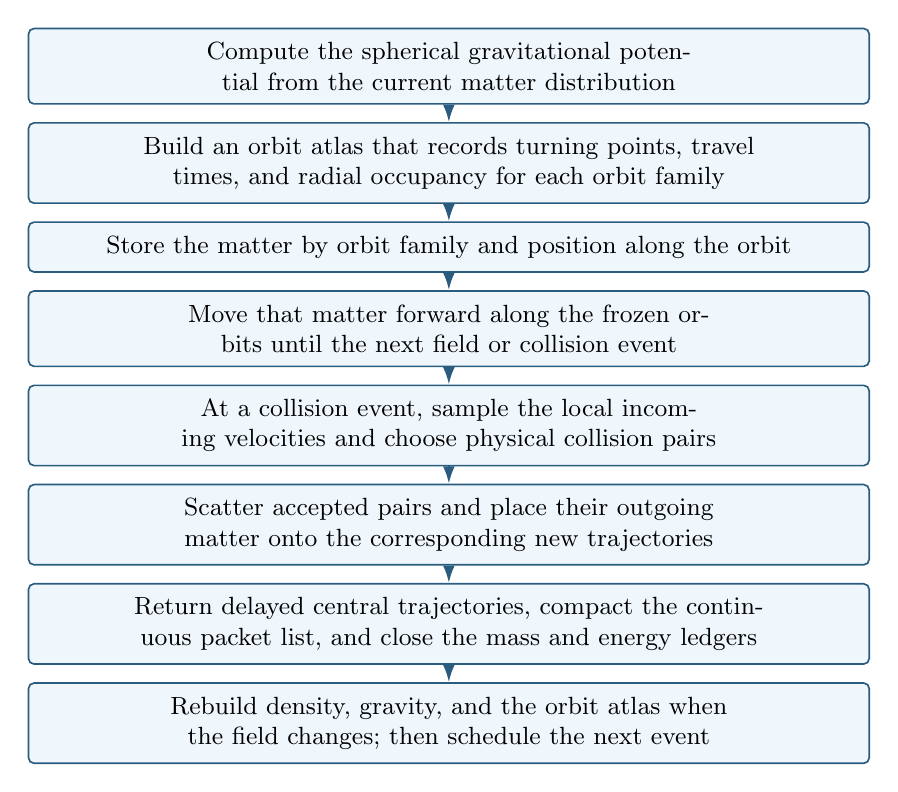
\begin{tikzpicture}[node distance=0.22cm]
\node[physicsflow] (cb1) {Compute the spherical gravitational potential from the current matter distribution};
\node[physicsflow,below=of cb1] (cb2) {Build an orbit atlas that records turning points, travel times, and radial occupancy for each orbit family};
\node[physicsflow,below=of cb2] (cb3) {Store the matter by orbit family and position along the orbit};
\node[physicsflow,below=of cb3] (cb4) {Move that matter forward along the frozen orbits until the next field or collision event};
\node[physicsflow,below=of cb4] (cb5) {At a collision event, sample the local incoming velocities and choose physical collision pairs};
\node[physicsflow,below=of cb5] (cb6) {Scatter accepted pairs and place their outgoing matter onto the corresponding new trajectories};
\node[physicsflow,below=of cb6] (cb7) {Return delayed central trajectories, compact the continuous packet list, and close the mass and energy ledgers};
\node[physicsflow,below=of cb7] (cb8) {Rebuild density, gravity, and the orbit atlas when the field changes; then schedule the next event};
\draw[physicsarrow] (cb1) -- (cb2);
\draw[physicsarrow] (cb2) -- (cb3);
\draw[physicsarrow] (cb3) -- (cb4);
\draw[physicsarrow] (cb4) -- (cb5);
\draw[physicsarrow] (cb5) -- (cb6);
\draw[physicsarrow] (cb6) -- (cb7);
\draw[physicsarrow] (cb7) -- (cb8);
\end{tikzpicture}
\end{figure}

\subsubsection{Purpose and state variables}

This module evolves a spherical SIDM distribution under self-gravity and
finite-angle elastic scattering.  Its state contains two connected
representations of the same physical system:
\begin{enumerate}
\item a finite-volume distribution on an orbit grid, used for long intervals
      of collisionless motion; and
\item continuous phase space packets created by recent collisions, used until
      they can be placed on the orbit grid with a conservative map.
\end{enumerate}

The implementation is organized in
\path{cpu/include/ev/canonical_orbit_phase_transport.hpp},
\path{cpu/include/ev/canonical_boltzmann_poisson_event.hpp}, and
\path{cpu/include/ev/weighted_vlasov_pic_collisions.hpp}.  Restarts are handled by
\path{cpu/include/ev/canonical_boltzmann_poisson_restart.hpp}.

In spherical symmetry we use
\[
  \eta=\frac{L^2}{2},\qquad
  H=\Phi(r)+\frac{w^2}{2}+\frac{\eta}{r^2}.             \tag{CBP1}
\]
Here \(w=v_r\), \(L=r v_t\), and \(H\) is the specific Hamiltonian in the
current gravitational potential.  The phase space measure is
\[
  \dd\Gamma=8\pi^2\,\dd r\,\dd w\,\dd\eta.             \tag{CBP2}
\]
The factor \(8\pi^2\) is included in every physical mass budget.

For a frozen spherical potential, \(\eta\) and \(H\) remain constant along an
orbit.  A third coordinate, the dimensionless radial phase
\(\zeta_{\rm orb}\in[0,1)\), tells us where the particle is between
pericentre and apocentre.  One radial period advances \(\zeta_{\rm orb}\) by
one.  The subscript distinguishes this orbit phase from the Schwarzschild time
\(\tau\) used in the relativistic chapters.  The orbit-grid coordinates are
therefore
\[
  (\eta,H,\zeta_{\rm orb}).                             \tag{CBP3}
\]

\noindent\textbf{Module interface.}
A dedicated caller initializes the canonical-orbit library.  The generic
\path{params.ini} interface selects the Eulerian methods described elsewhere.
The canonical initializer takes a cell-integrated distribution, an equilibrium
table \(f(H)\), the resolution of the orbit atlas, collision-shell controls,
field and collision clocks, and an output directory.  A continuation additionally reads the canonical restart,
which stores the atlas, continuous packets, random counters, and both event
clocks.  The task-specific Eulerian finite-angle frontends described in
Section~\ref{sec:eulerian-grid-collisions} are separate algorithms and must
not be used as substitutes for this orbit-atlas representation.

\subsubsection{Building the canonical orbit atlas}

The orbit atlas tabulates the bound trajectories represented by the
finite-volume cells in equation~(CBP3).  Its construction first fixes angular
momentum and energy, then resolves orbital phase and the overlap with the
collision grid.  These four steps are described below.

\paragraph{Step 1: angular momentum planes.}

Each Eulerian \(\eta\) cell is integrated with a small Gaussian rule.  The
first cell uses a left Gauss--Radau rule, so one plane lies exactly at
\(\eta=0\).  The last cell uses a right Gauss--Radau rule.  Interior cells use
Gauss--Legendre points.  These endpoint planes give direct support to radial
orbits and to the largest represented angular momentum.

The rule selection appears in the atlas builder:
\codesource{Canonical orbit-atlas angular momentum quadrature}
{\path{cpu/include/ev/canonical_orbit_phase_transport.hpp};
 \path{cpu/include/ev/phase_space_cells.hpp}}
{Chooses endpoint-inclusive Gauss--Radau planes at the two angular momentum
 boundaries and Gauss--Legendre planes in interior cells}
\begin{lstlisting}[language=C++]
if (eta_cell == 0)
  return phase_space_gauss_radau_left_rule(points);
if (eta_cell == p.NL - 1)
  return phase_space_gauss_radau_right_rule(points);
return phase_space_gauss_legendre_rule(points);
\end{lstlisting}

\paragraph{Step 2: energy rows.}

At fixed \(\eta\), define the effective potential
\[
  \Phi_{\rm eff}(r;\eta)=\Phi(r)+\frac{\eta}{r^2}.       \tag{CBP4}
\]
For a bound orbit with energy \(H\), the turning points solve
\(\Phi_{\rm eff}=H\).  The inner turning radius
\(r_p\) is the pericentre, and the outer turning radius \(r_a\) is the
apocentre; radial motion is allowed for \(r_p\le r\le r_a\).  The radial
action is
\[
  J_r(H,\eta)=\frac{1}{\pi}
  \int_{r_p}^{r_a}\sqrt{2[H-\Phi_{\rm eff}(r;\eta)]}\,\dd r.  \tag{CBP5}
\]
Energy-row faces are placed through monotone edges in \(J_r\).  An optional
positive weight based on the initial \(f(H,\eta)\) concentrates rows where
the phase space mass is large.  The row stores both its action interval and
its energy interval.  During a later Poisson rebuild, the action edges define
the corresponding energy edges in the new potential.

\paragraph{Step 3: phase cells.}

For one representative orbit, let \(T_r\) be the radial period.  The orbit
phase is elapsed orbital time normalized by this period,
\[
  \zeta_{\rm orb}=\frac{t_{\rm orbit}}{T_r}\pmod 1,
  \qquad \dot\zeta_{\rm orb}=\frac{1}{T_r}.             \tag{CBP6}
\]
Each energy row is divided into equal intervals in \(\zeta_{\rm orb}\).
Equal phase width means equal residence-time width.  Dense sampling near a
turning point then arises from the orbit map itself, where a fixed time
interval covers a small radial interval.

\paragraph{Step 4: overlap with the collision grid.}

Density, pressure, collisions, and the Poisson solve use the Eulerian cells
\((r,w,\eta)\).  The atlas builder traces the boundary of each canonical cell
into the \((r,w)\) plane and intersects it with the Eulerian rectangles.  For
each intersection it stores
\[
  \int\dd\Gamma,\qquad
  \int H\,\dd\Gamma,\qquad
  \int H^2\,\dd\Gamma,                                  \tag{CBP7}
\]
together with the geometric moments needed by the quadratic reconstruction.
These overlaps are computed once for one frozen potential and reused by all
projections in that interval.

\begin{figure}[ht]
\centering
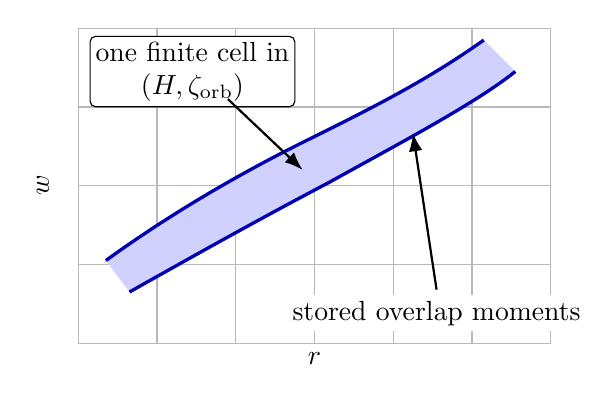
\begin{tikzpicture}[x=1.0cm,y=1.0cm,>=Latex]
  \draw[step=1cm,gray!55,thin] (0,0) grid (6,4);
  \node[below] at (3,0) {$r$};
  \node[rotate=90] at (-0.45,2) {$w$};
  \fill[blue!18]
    (0.65,0.65) .. controls (1.45,1.10) and (2.25,1.55) ..
    (3.20,2.05) .. controls (4.10,2.55) and (5.05,3.05) ..
    (5.55,3.45) --
    (5.15,3.85) .. controls (4.35,3.28) and (3.55,2.90) ..
    (2.75,2.50) .. controls (1.80,2.02) and (1.00,1.52) ..
    (0.35,1.05) -- cycle;
  \draw[blue!70!black,very thick]
    (0.65,0.65) .. controls (1.45,1.10) and (2.25,1.55) ..
    (3.20,2.05) .. controls (4.10,2.55) and (5.05,3.05) ..
    (5.55,3.45);
  \draw[blue!70!black,very thick]
    (0.35,1.05) .. controls (1.00,1.52) and (1.80,2.02) ..
    (2.75,2.50) .. controls (3.55,2.90) and (4.35,3.28) ..
    (5.15,3.85);
  \node[fill=white,draw,rounded corners=2pt,align=center,inner sep=2pt]
    at (1.45,3.45)
    {one finite cell in\\$ (H,\zeta_{\rm orb}) $};
  \draw[->,thick] (1.90,3.10) -- (2.85,2.20);
  \node[align=center,fill=white,inner sep=2pt] at (4.55,0.38)
    {stored overlap moments};
  \draw[->,thick] (4.55,0.68) -- (4.25,2.67);
\end{tikzpicture}
\caption{One canonical cell mapped into the Eulerian \((r,w)\) plane at fixed
\(\eta\).  Its curved image crosses several rectangles.  VENUS stores the
integral over each shaded intersection, so later projections use integrated
mass instead of a single sample point.}
\label{fig:canonical-atlas-overlap}
\end{figure}

Each canonical phase cell stores three integrated quantities,
\[
  M_c=\int_c f\,\dd\Gamma,\qquad
  E_c=\int_c Hf\,\dd\Gamma,\qquad
  E_{2,c}=\int_c H^2f\,\dd\Gamma.                        \tag{CBP8}
\]
They retain the mean and variance of \(H\) inside an energy row.  A quadratic
reconstruction in \(H\) can therefore be projected without replacing the row
by its center energy.  Positivity is checked from the reconstructed value;
the stored cell moments are also checked against the exact moment bounds for
the interval \([H_L,H_R]\):
\[
 H_L\le \langle H\rangle\le H_R,\qquad
 \langle H\rangle^2\le\langle H^2\rangle
 \le(H_L+H_R)\langle H\rangle-H_LH_R.                  \tag{CBP9}
\]

\subsubsection{Frozen-potential Vlasov transport}

During a frozen-field interval, each row advances by a phase shift,
\[
  \zeta_{\rm orb}\longmapsto
  \zeta_{\rm orb}+\frac{\Delta t}{T_r}\pmod 1.         \tag{CBP10}
\]
The finite-volume masses and Hamiltonian moments stay in their canonical
cells.  The row stores the accumulated shift in \code{phase_offset}:
\codesource{Canonical frozen-orbit phase transport}
{\path{cpu/include/ev/canonical_orbit_phase_transport.hpp}}
{Advances each orbit row by its period-normalized phase translation and wraps
 the result onto the unit radial-phase interval}
\begin{lstlisting}[language=C++]
row.phase_offset = hamiltonian_orbit_wrap_phase(
    row.phase_offset + dt / row.period);
\end{lstlisting}

This update is an exact translation for the representative orbit in the
frozen potential.  Projection to \((r,w,\eta)\) is performed when moments or
collisions are required.  Consequently many orbital intervals can be
accumulated before a new reconstruction is needed.

Nearly radial trajectories use the regularized orbit geometry in
\path{cpu/include/ev/hamiltonian_orbit_phase.hpp}.  The ordinary integrator is
used when its energy check passes.  A failed check triggers the
Levi--Civita-style regularized evaluation near pericentre.  The orbit table
records retry and unresolved-orbit diagnostics.

\subsubsection{The finite inner radius}
\label{sec:delayed-inner-carrier}

The logarithmic radial mesh begins at \(R=r_{\min}>0\).  An orbit that enters
\(0<r<R\) keeps evolving in the central potential.  Its canonical phase map
contains a hidden phase interval whose duration is the physical inward and
outward flight time.  Mass in this phase interval is included in the enclosed
mass used by Poisson.  When the phase reaches the outgoing crossing, the same
orbit returns through \(R\) with outward radial velocity.

The resolved and hidden pieces obey
\[
 M_{\rm atlas}=M_{\rm visible}+M_{\rm hidden}+M_{\rm escaped}. \tag{CBP11}
\]
The code checks this partition for every canonical column.  SIDM calculations
also report the optical depth across \(0<r<R\) and are repeated with smaller
\(R\).

\subsubsection{Choosing the next event time}

The potential and collision clocks are independent.  From consecutive
Poisson fields, VENUS estimates a mass-weighted field-change time using both
\(\Phi\) and \(g=\partial_r\Phi\).  The requested field interval is a fraction
\(\epsilon_\Phi\) of that time.  The collision module supplies a physical
collision time and an NTC-majorant time.  The scheduler uses
\[
 \Delta t=\min\left(
  \Delta t_{\max},
  \epsilon_\Phi t_\Phi-t_{\Phi,{\rm age}},
  \epsilon_C t_C-t_{C,{\rm age}},
  \epsilon_{\rm maj}t_{\rm maj}
 \right).                                               \tag{CBP12}
\]
Here \(\Delta t_{\max}\) is the configured hard cap;
\(t_\Phi\) is the mass-weighted field-change timescale, and
\(t_{\Phi,{\rm age}}\) is the elapsed time since the last potential rebuild.
The derivative estimate is the smaller of
\(\sqrt{\sum_i\omega_i\Phi_i^2/\sum_i\omega_i\dot\Phi_i^2}\) and
\(\sqrt{\sum_i\omega_i g_i^2/\sum_i\omega_i\dot g_i^2}\), where
\(g=\Phi_r\), \(M_i=4\pi\max(\rho_i,0)
(r_{i+1/2}^3-r_{i-1/2}^3)/3\) is nonnegative resolved shell mass, and
\(\omega_i=M_i/(M_{\rm hidden}+\sum_jM_j)\).
Here \(M_{\rm hidden}\) is the unresolved inner mass in (CBP11), and the
rates follow from \code{vp_potential_time_derivative}.  Each channel requires
both mean squares to exceed \((4096\epsilon_{\rm mach})^2\), with
\(\epsilon_{\rm mach}\) double-precision machine roundoff. A channel at or
below this threshold gives infinite time, as do zero total mass and the
helper's expanding-background branch.
After an event the solver also restricts \(t_\Phi\) by the elapsed field time
divided by the larger mass-weighted relative potential or force change
returned by \code{canonical_field_mismatch}.  These are the distinct
canonical helpers in \path{cpu/include/ev/canonical_boltzmann_poisson_event.hpp},
lines 242--418 and 1801--1835.
Likewise \(t_C\) is the minimum local physical
collision timescale and \(t_{C,{\rm age}}\) is the elapsed time since the
last collision event.  The dimensionless fractions \(\epsilon_\Phi\) and
\(\epsilon_C\) set the corresponding deadlines.  Finally,
\(t_{\rm maj}\) is the no-time-counter (NTC) proposal-majorant timescale and
\(\epsilon_{\rm maj}\) is its safety fraction.  Subtracting each age prevents
one kind of event from indefinitely postponing the other.

The source call is:
\codesource{Canonical Boltzmann--Poisson event scheduler}
{\path{cpu/include/ev/canonical_boltzmann_poisson_event.hpp};
 \path{cpu/include/ev/weighted_vlasov_pic_event_scheduler.hpp}}
{Combines the independent field and collision clock ages with their physical
 deadlines to choose the next event interval and ordering}
\begin{lstlisting}[language=C++]
diagnostics.plan = plan_weighted_pic_event(
    {state.potential_age, state.collision_age},
    state.potential_timescale,
    scheduled_collision_timescale,
    options.potential_fraction,
    options.collision_fraction,
    maximum_interval);
\end{lstlisting}

If the collision clock expires first, the sequence is orbit advance,
collision, and later field rebuild.  If the field clock expires first, the
sequence is orbit advance, field rebuild, and later collision.  When both
expire together, the scheduler records their chronological order and executes
both operations at the same event time.

\subsubsection{Sampling the instantaneous distribution}

At a collision event, the atlas and all active continuous packets are sampled
at their current phase.  A sampled marker contains
\[
  (r,w,v_{t,1},v_{t,2},m_p).                             \tag{CBP13}
\]
The tangential direction is uniform in its local plane.  Marker weights are
fractional, so a canonical cell can contribute to several independent virtual
batches.  Increasing the number of markers improves the estimate of the local
collision integral without changing the orbit-grid resolution.

Markers are sorted by radius and divided into disjoint shells.  A shell is
accepted for local scattering when
\[
  \Delta r_s\le\lambda_{\rm rms,s}.                     \tag{CBP14}
\]
The shell builder can increase its population to reduce statistical noise.
The ledger records the shell width, mean free path, marker count, and the
largest ratio \(\Delta r_s/\lambda_{\rm rms,s}\).

\subsubsection{No-time-counter pair selection}

Consider one shell of volume \(V_s\), density \(\rho_s\), and \(N_s\) sampled
markers.  Define
\[
  A_s\ge \max_{i,j}\left[u_{ij}\sigma_{\rm tot}(u_{ij})\right],
  \qquad u_{ij}=|\boldsymbol v_i-\boldsymbol v_j|.       \tag{CBP15}
\]
The no-time-counter clock proposes unordered pairs at rate
\[
  \nu_{{\rm trial},s}=\frac{N_s-1}{2}\rho_s A_s.        \tag{CBP16}
\]
For every proposal, two distinct marker indices are drawn uniformly.  With a
fresh uniform random number \(U_a\in(0,1)\), the pair is accepted when
\[
  U_a A_s<u_{ij}\sigma_{\rm tot}(u_{ij}).               \tag{CBP17}
\]
Equations~(CBP16)--(CBP17) give the required rate
\(f_i f_j u_{ij}\sigma_{\rm tot}\) in expectation.  The algorithm visits the
realized proposals and accepted events.  Its cost scales with the physical
trial count.

The implementation follows these equations directly:
\codesource{Canonical-orbit no-time-counter sampler}
{\path{cpu/include/ev/canonical_orbit_phase_transport.hpp}}
{Draws distinct local phase space samples and accepts each trial against the
 shell's verified relative-speed--cross-section majorant}
\begin{lstlisting}[language=C++]
clock += -std::log(rng.uniform_open()) / trial_rate;
ia = rng.uniform_index(count);
ib = draw_distinct_index(count, ia);
u_sigma = relative_speed * total_cross_section_per_mass(...);
if (rng.uniform_open() * shell.majorant_u_sigma >= u_sigma)
  continue;
\end{lstlisting}

\subsubsection{Drawing the outgoing direction}

Let
\[
 \boldsymbol V=\frac{\boldsymbol v_1+\boldsymbol v_2}{2},
 \qquad \boldsymbol u=\boldsymbol v_1-\boldsymbol v_2. \tag{CBP18}
\]
Elastic scattering changes the direction of \(\boldsymbol u\) and keeps its
magnitude.  Write \(\mu=\cos\theta\).  The normalized cumulative distribution
for \(\mu\) is
\[
 P(\mu\le x)=
 \frac{2\pi}{\sigma_{\rm tot}(u)}
 \int_{-1}^{x}\frac{\dd\sigma}{\dd\Omega}(u,\mu')\,\dd\mu'. \tag{CBP19}
\]
VENUS draws \(U_\mu\in(0,1)\) and inverts equation~(CBP19).  Isotropic
scattering gives \(\mu=2U_\mu-1\).  For the Born Yukawa kernel, the analytic
inverse used by the code is
\[
 a=m_\phi^2,\qquad b=\frac{m_\chi^2u^2}{2},
\]
\[
 y=\frac{2b}{a},\qquad
 \mu=1-\frac{2U_\mu}{1+y(1-U_\mu)}.                     \tag{CBP20}
\]
Here \(U_\mu\) samples the probability of a cosine at or above \(\mu\),
complementary to the increasing cumulative probability in (CBP19).
This factored expression has the continuous uniform-cosine limit
\(\mu=1-2U_\mu\) at \(y=0\); the numerical inverse uses \(1/y\) when
\(y>1\) to keep the arithmetic bounded.
A second independent random number gives the azimuth
\(\psi=2\pi U_\psi\).  The code constructs the unit vector
\(\widehat{\boldsymbol u}'(\mu,\psi)\) around the incoming relative direction
and sets
\[
 \boldsymbol v'_1=\boldsymbol V+\frac{u}{2}
       \widehat{\boldsymbol u}',\qquad
 \boldsymbol v'_2=\boldsymbol V-\frac{u}{2}
       \widehat{\boldsymbol u}'.                        \tag{CBP21}
\]
Thus each accepted pair satisfies
\[
 \boldsymbol v'_1+\boldsymbol v'_2=\boldsymbol v_1+\boldsymbol v_2,
 \qquad
 |\boldsymbol v'_1|^2+|\boldsymbol v'_2|^2
 =|\boldsymbol v_1|^2+|\boldsymbol v_2|^2.              \tag{CBP22}
\]

The corresponding source excerpt is:
\codesource{Finite-angle elastic-scattering map}
{\path{cpu/include/ev/weighted_vlasov_pic_collisions.hpp};
 \path{cpu/include/ev/finite_angle_boltzmann.hpp}}
{Samples the scattering cosine and azimuth and constructs the two outgoing
 centre-of-mass-frame velocities while preserving pair invariants}
\begin{lstlisting}[language=C++]
const double mu = sample_scatter_mu(u, p, options, rng);
const double psi = 2.0 * PI * rng.uniform_open();
const BPFAVec3 direction =
    bp_fa_scattered_relative_direction(relative, mu, psi);
const BPFAVec3 relative_after = bp_fa_scale(direction, u);
const BPFAVec3 out1 = bp_fa_add(centre,
    bp_fa_scale(relative_after, 0.5));
const BPFAVec3 out2 = bp_fa_sub(centre,
    bp_fa_scale(relative_after, 0.5));
\end{lstlisting}

Both tangential components enter equation~(CBP21).  After scattering, the
new angular momentum of each packet is
\[
 L'=r\sqrt{(v'_{t,1})^2+(v'_{t,2})^2},\qquad
 \eta'=\frac{(L')^2}{2}.                                \tag{CBP23}
\]
Collisions therefore redistribute angular momentum while preserving the full
three-dimensional pair momentum and kinetic energy.

\subsubsection{Gain, loss, and reverse events}

An accepted event contains its incoming and outgoing velocities in one
record.  The incoming mass is withdrawn from the canonical cells that owned
the sampled marker.  The two outgoing packets are then created with the same
event mass.  This is the sampled gain-minus-loss update of the Boltzmann
operator.

The collision map in equation~(CBP21) is one-to-one and preserves velocity
volume.  Drawing \(\psi\) over the full interval and drawing \(\mu\) from the
complete differential cross section includes the reverse map with its
physical probability.  For a Maxwellian \(f_M\propto\exp(-v^2/2T)\), equation
(CBP22) gives
\[
 f_M(\boldsymbol v_1)f_M(\boldsymbol v_2)
 =f_M(\boldsymbol v'_1)f_M(\boldsymbol v'_2).            \tag{CBP24}
\]
The expected collision update therefore vanishes.  A numerical realization
should approach this null state as the collision-marker population and orbit
atlas are refined.

\subsubsection{Source-owned withdrawal and outgoing carriers}

Each sampled canonical marker keeps the finite-volume cells and weights that
created it.  Once a pair is accepted, the incoming event mass is removed from
those owned cells immediately.  The source cells move with the frozen-field
phase flow, so this withdrawal includes their resolved and hidden orbital
phases consistently.

The outgoing velocities define continuous packets at the collision radius.
They are advanced along their new orbits until the next collision event.  The
main source sequence is:
\codesource{Canonical source withdrawal and outgoing carriers}
{\path{cpu/include/ev/canonical_orbit_phase_transport.hpp}}
{Removes accepted incoming mass from its owned atlas cells and retains the
 two outgoing continuous packets for conservative remapping onto new orbits}
\begin{lstlisting}[language=C++]
represented_first_before = withdraw_source(
    pair.first_ref, pair.first_source,
    event.first_before, packet_mass);
represented_second_before = withdraw_source(
    pair.second_ref, pair.second_source,
    event.second_before, packet_mass);

retain_signed_marker(new_signed_positive,
    collision_source[pair.first_source],
    event.first_after, packet_mass);
retain_signed_marker(new_signed_positive,
    collision_source[pair.second_source],
    event.second_after, packet_mass);
\end{lstlisting}

At creation, the atlas loss and outgoing packet gain satisfy
\[
 \Delta M_{\rm atlas}+M_{\rm outgoing}=0.              \tag{CBP25}
\]
The pair ledger also checks equation~(CBP22) for every accepted event.

\subsubsection{Mapping outgoing packets onto the orbit grid}

Before the next collision distribution is sampled, active outgoing packets
are placed on the current atlas:
\begin{enumerate}
\item Compute \(\eta'\) and \(H'\) from equations~(CBP1) and (CBP23).
\item Find the two neighboring \(\eta\) quadrature planes with positive linear
      weights.
\item Find the energy row containing \(H'\) on each plane.
\item Integrate the orbit to obtain the physical phase
      \(\zeta_{\rm orb}'\).
\item Convert \(\zeta_{\rm orb}'\) to the co-moving phase coordinate using the row's
      current \code{phase_offset}.
\item Deposit mass, \(H\)-mass, and \(H^2\)-mass with positive weights into at
      most four neighboring canonical cells.
\end{enumerate}

The deposition weights sum to one.  The materialization transaction checks
mass before committing it.  It also checks the moment bounds in
equation~(CBP9).

An outgoing packet with \(H'>0\) lies above the bound-orbit atlas.  It remains
an explicit open-orbit packet.  The characteristic integrator advances it,
the collision sampler includes it while it is inside the radial domain, and
the escape ledger records it after it crosses the outer boundary.  Separate
counters classify open packets caused by high energy, angular momentum
support, a missing row, an energy gap, or an orbit-geometry failure.

\subsubsection{Keeping the continuous packet list compact}

Many small collision packets may occupy nearly the same local phase space
region.  VENUS replaces each such group by a positive quadrature supported on
a subset of the existing packet locations.  Positions and velocities remain
physical packet states.  The new nonnegative weights preserve fourteen group
moments:
\begin{align*}
&1, q, w, qw, w^2, qw^2, v_t^2, qv_t^2,\\
&\frac{v^2}{2}w, q\frac{v^2}{2}w,
 \eta, q\eta, H, H^2,\qquad q=\frac{r^3}{3}.          \tag{CBP26}
\end{align*}
These constraints preserve mass, radial momentum, radial and tangential
kinetic moments, radial kinetic-energy flux, the squared-angular momentum
moment \(\eta=L^2/2\), and the first
two Hamiltonian moments.  The factors with \(q\) preserve the same quantities
under radial cloud-in-cell deposition.

The reduction is local in \((r,w,\eta)\).  A group contains packets with the
same deposition stencil.  A Carath\'eodory reduction is a positive
convex-geometry compression: it replaces a nonnegative weighted cloud by a
subset of its existing packet locations while preserving the requested
moment vector.  It leaves at most fourteen packets in a well-conditioned
group.  Here ``well-conditioned'' means that the retained moment columns are
sufficiently independent for their nonnegative weights to be solved without
amplifying roundoff.  Every group recomputes equation~(CBP26) after reduction.
A group whose moment matrix is ill-conditioned or whose residual exceeds the
requested tolerance keeps its original packets.

Packet ordering is made deterministic from marker identity and phase space
coordinates before the reduction, so a fixed platform and random seed retain
the same packet order across supported OpenMP thread counts.

\subsubsection{Refreshing the gravitational field}

When the field clock expires, VENUS projects the instantaneous atlas and
continuous packets to radial moments and solves spherical Poisson.  A new
orbit atlas is built in the new potential with the previous radial-action
edges.  Mass and its \((H,H^2)\) moments are transferred between matching
topological rows.  The field iteration stops when the mass-weighted mismatch
between the represented field and a fresh Poisson solve is below tolerance.

This rebuild lets the slowly changing stationary part of \(f(H,\eta)\) evolve
with the potential.  The current distribution supplies the transferred row
moments; the initial equilibrium table is used only for initialization.

\subsubsection{Conservation diagnostics and output}

Every event writes the following independent checks:
\begin{itemize}
\item atlas mass before and after frozen transport;
\item represented mass before and after collisions;
\item pair momentum and kinetic-energy errors;
\item shell locality \(\Delta r_s/\lambda_{\rm rms,s}\);
\item materialization residuals in \(M\), \(H\), and \(H^2\);
\item packet-compression moment residuals;
\item active, hidden, and escaped open-orbit mass;
\item field mismatch and the measured potential-change time;
\item marker-batch estimates of density and radial heat-flux noise.
\end{itemize}

The main files are \path{history.csv}, \path{profiles.csv}, and
\path{operator_mass_budget.csv}.  A restart stores the atlas, phase offsets,
all three cell moments, open packets, deferred outgoing packets, random-stream
counters, and both event clocks.

Convergence studies should vary the orbit-grid resolution, marker count,
virtual collision batches, local shell population, compression subcells,
\(r_{\min}\), and the allowed active open-tail fraction.  The comparison uses
density, radial velocity dispersion, collision energy transfer, and radial
heat flux.  A gravothermal core-collapse comparison should additionally
resolve the early dilution, subsequent reversal, and central-density growth
through the chosen physical interval.


\subsection{Cell-Integrated Conservative Semi-Lagrangian Transport}
\label{sec:cell-integrated-sldg}

\begin{figure}[htbp]
\centering
\textbf{Physics flow: cell-integrated conservative semi-Lagrangian module}
\par\smallskip
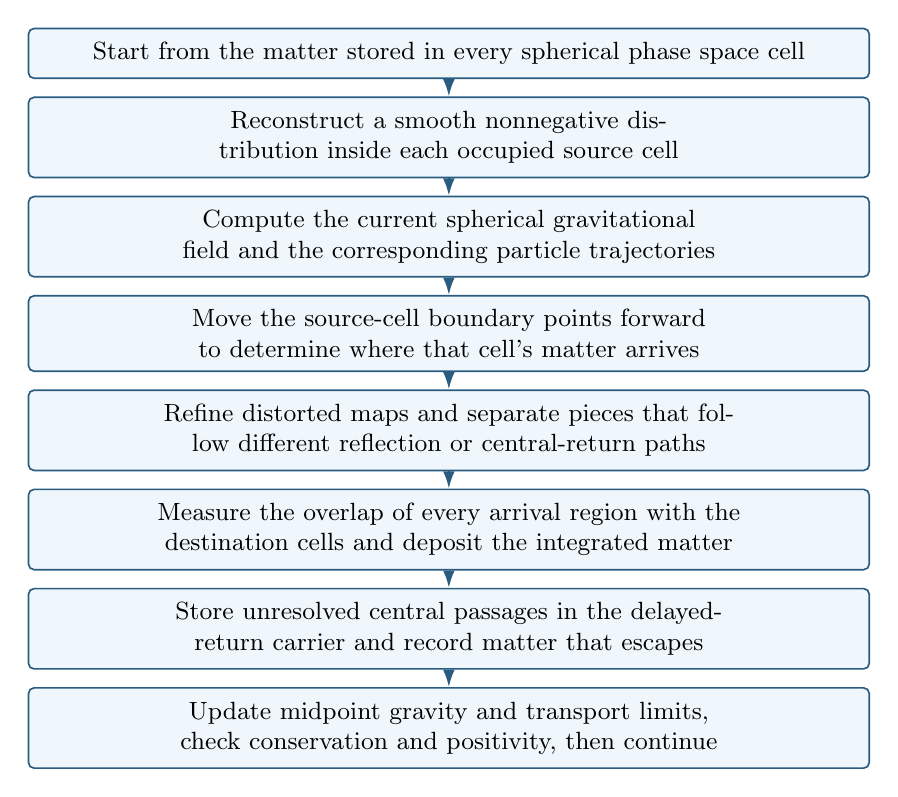
\begin{tikzpicture}[node distance=0.22cm]
\node[physicsflow] (sl1) {Start from the matter stored in every spherical phase space cell};
\node[physicsflow,below=of sl1] (sl2) {Reconstruct a smooth nonnegative distribution inside each occupied source cell};
\node[physicsflow,below=of sl2] (sl3) {Compute the current spherical gravitational field and the corresponding particle trajectories};
\node[physicsflow,below=of sl3] (sl4) {Move the source-cell boundary points forward to determine where that cell's matter arrives};
\node[physicsflow,below=of sl4] (sl5) {Refine distorted maps and separate pieces that follow different reflection or central-return paths};
\node[physicsflow,below=of sl5] (sl6) {Measure the overlap of every arrival region with the destination cells and deposit the integrated matter};
\node[physicsflow,below=of sl6] (sl7) {Store unresolved central passages in the delayed-return carrier and record matter that escapes};
\node[physicsflow,below=of sl7] (sl8) {Update midpoint gravity and transport limits, check conservation and positivity, then continue};
\draw[physicsarrow] (sl1) -- (sl2);
\draw[physicsarrow] (sl2) -- (sl3);
\draw[physicsarrow] (sl3) -- (sl4);
\draw[physicsarrow] (sl4) -- (sl5);
\draw[physicsarrow] (sl5) -- (sl6);
\draw[physicsarrow] (sl6) -- (sl7);
\draw[physicsarrow] (sl7) -- (sl8);
\end{tikzpicture}
\end{figure}

\subsubsection{Purpose and distinction from nodal pullback}

The cell-integrated semi-Lagrangian discontinuous-Galerkin module is the
conservative spherical Vlasov--Poisson transport path.  In this manual,
\emph{semi-Lagrangian} means that the numerical
method follows phase space characteristics over a finite time interval.
\emph{Discontinuous Galerkin} means that the distribution is represented by a
separate polynomial inside every phase space cell; the polynomial is allowed
to jump across cell faces.  The abbreviation SLDG will be used for this
cell-integrated semi-Lagrangian discontinuous-Galerkin method.

The implemented state is a cell average
\[
 \bar f_{ijk}
 =\frac{1}{\Delta r_i\Delta w_j\Delta\eta_k}
   \int_{I_i}\!\dd r\int_{J_j}\!\dd w\int_{K_k}\!\dd\eta\,
   f(r,w,\eta),
 \qquad \eta\equiv\frac{L^2}{2}.
\]
Here \(I_i=[r_{i-1/2},r_{i+1/2}]\), \(J_j=[w_{j-1/2},w_{j+1/2}]\),
and \(K_k=[\eta_{k-1/2},\eta_{k+1/2}]\) are one radial, radial-velocity,
and angular momentum cell.  The symbols
\(\Delta r_i\), \(\Delta w_j\), and \(\Delta\eta_k\) denote their widths.
Since \(L\,\dd L=\dd\eta\), the physical phase space measure is
\[
 \dd\Gamma=8\pi^2\,\dd r\,\dd w\,\dd\eta,
 \qquad
 M_{ijk}=8\pi^2\bar f_{ijk}
          \Delta r_i\Delta w_j\Delta\eta_k .
\]
The factor \(8\pi^2\) results from integrating the two configuration-space
angles and the unused velocity azimuth under spherical symmetry.

The nodal semi-Lagrangian method traces each target grid point back to its
departure point and interpolates \(f\) there.  The SLDG method transports
integrated mass: it reconstructs every \emph{source cell}, maps that cell
forward, and integrates its overlap with the destination cells.  This
source-to-destination accounting gives the conservative update
\[
 M^{n+1}_{abc}
 =\sum_{ijk}
   \int_{\mathcal A_{ijk}\cap D_{abc}}
   f^n_{h,ijk}\circ\mathcal X^{-1}\,
   8\pi^2\,\dd r\,\dd w\,\dd\eta ,
\]
where \(\mathcal X\) is the characteristic map from time \(t^n\) to
\(t^{n+1}\), \(\mathcal A_{ijk}=\mathcal X(I_i\times J_j\times K_k)\)
is an arrival region, \(D_{abc}\) is a destination cell, and
\(f^n_{h,ijk}\) is the reconstructed source polynomial.  There is no
post-step global mass rescaling.  Source mass outside the visible grid is
recorded either in the delayed-inner carrier, which stores unresolved central
passages, or in the escape budget.  Together these destinations account for
the complete transported mass.

The relevant sources are:
\begin{itemize}
\item \path{cpu/include/ev/conservative_sldg_transport.hpp}: polynomial
reconstruction, mapped-polygon geometry, recursive refinement, exact overlap
integration, delayed-return coupling, and midpoint-field driver;
\item \path{cpu/include/ev/hamiltonian_sldg_transport.hpp}: Hamiltonian-aligned
reconstruction, cached modal state, and static-potential timestep control;
\item \path{cpu/include/ev/hamiltonian_orbit_reference.hpp}: optional positive
orbit-average reference \(f_0(H,\eta)\);
\item \path{cpu/include/ev/delayed_inner_orbit_carrier.hpp}: persistent
finite-volume mass inside \(0<r<r_{\min}\);
\item \path{cpu/include/ev/radial_orbit_regularization.hpp}: selective
Levi--Civita characteristic retry near stiff pericentres.
\end{itemize}

\subsubsection{Frozen spherical Hamiltonian map}

For static spherical Vlasov--Poisson evolution at fixed
\(\eta=L^2/2\), the one-particle Hamiltonian is
\[
 H(r,w;\eta)
 =\frac{w^2}{2}+\frac{\eta}{r^2}+\Phi(r).
\]
Here \(w=\dot r\) is radial velocity, \(L\) is the magnitude of specific
angular momentum, \(\Phi\) is the gravitational potential, and
\(\eta/r^2=L^2/(2r^2)\) is tangential kinetic energy.  The characteristic
equations are
\[
 \dot r = \frac{\partial H}{\partial w}=w,
 \qquad
 \dot w =-\frac{\partial H}{\partial r}
 =\frac{2\eta}{r^3}-\Phi_r,
 \qquad
 \dot\eta=0,
\]
where \(\Phi_r=\partial\Phi/\partial r\).  Hamiltonian flow preserves
phase space area:
\[
 \det\!\left(\frac{\partial(r',w')}{\partial(r,w)}\right)=1,
 \qquad
 \dd r'\,\dd w'=\dd r\,\dd w .
\]
This area preservation is both a physical property and a numerical geometry
check.  For a small source patch with area \(A_0\), the mapped corner polygon
should have area \(A\simeq A_0\).  VENUS records the relative area defect
\[
 \epsilon_A=\frac{|A-A_0|}{A_0}.
\]

The default characteristic update inside the SLDG map is
kick--drift--kick (KDK).  If
\[
 a_r(r;\eta) = \frac{2\eta}{r^3}-\Phi_r(r)
\]
denotes radial acceleration in the frozen field, one KDK step is
\[
 w^{n+1/2}=w^n+\frac{\Delta t}{2}a_r(r^n;\eta),
\quad
 r^{n+1}=r^n+\Delta t\,w^{n+1/2},
\quad
 w^{n+1}=w^{n+1/2}
 +\frac{\Delta t}{2}a_r(r^{n+1};\eta).
\]
The exact implementation also resolves the selected radial boundary and may
retry a stiff pericentre segment with the Levi--Civita transformation described
in the orbit-regularization module reference below.  The frozen-field map is used
only within one transport evaluation; self-gravity is time-centred as
described below.

\subsubsection{P2 source polynomial and its cell average}

Inside one \((r,w)\) source cell at a fixed \(\eta\) quadrature node, define
normalized coordinates
\[
 x=\frac{r-r_i}{\Delta r_i},
 \qquad
 y=\frac{w-w_j}{\Delta w_j},
 \qquad -\frac12\le x,y\le\frac12 .
\]
The notation \(P_2\) means the six-dimensional space of polynomials in
\((x,y)\) whose total degree is at most two: one constant, two linear, and
three quadratic modes.  The implemented \(P_2\) polynomial is
\begin{equation*}
 \begin{split}
 f_h(x,y)={}&\bar f
 +a_r x+a_w y
 +a_{rr}\left(x^2-\frac1{12}\right)\\
 &+a_{rw}xy
 +a_{ww}\left(y^2-\frac1{12}\right).
 \end{split}
 \tag{SLDG-P2}\label{eq:sldg-p2}
\end{equation*}
All symbols in this expression are local to one source cell:
\(\bar f\) is the stored cell average; \(a_r,a_w\) are linear modes;
\(a_{rr},a_{rw},a_{ww}\) are quadratic modes.  Since
\[
 \int_{-1/2}^{1/2}x\,\dd x=0,
 \qquad
 \int_{-1/2}^{1/2}\left(x^2-\frac1{12}\right)\dd x=0,
\]
and similarly for \(y\), every nonconstant mode has zero mean.  Therefore the
polynomial integrates to \(\bar f\Delta r_i\Delta w_j\) independently of
the slope and curvature values.

The plain conservative SLDG mode currently constructs limited linear slopes.
For a cell-centred sequence \(q_i\), the minmod limiter is
\[
 \operatorname{minmod}(a,b,c)=
 \begin{cases}
  \min(a,b,c),&a,b,c>0,\\
  \max(a,b,c),&a,b,c<0,\\
  0,&\text{otherwise},
 \end{cases}
\]
and the radial slope is obtained from the backward, centred, and forward
differences with the usual factor-of-two bounds.  The same construction is
used in \(w\). At a wall of fixed physical radius \(R\), the reflecting
radial ghost state is evaluated at \(w'=-w-2HR\), where \(H\) is the
Hubble rate. The static limit \(H=0\) gives \(w'=-w\).

The source representation in
\path{cpu/include/ev/conservative_sldg_transport.hpp} is:
\codesource{Conservative SLDG source polynomial}
{\path{cpu/include/ev/conservative_sldg_transport.hpp}}
{Stores the cell average and five local quadratic modes and applies the
 source-cell positivity limiter before forward transport}
\begin{lstlisting}[language=C++]
struct SLDGSourcePolynomial {
  double cell_average = 0.0;
  std::array<double, 5> mode{};
  double center_r = 0.0, center_w = 0.0;
  double scale_r = 1.0, scale_w = 1.0;
  double enforce_positivity();
};
\end{lstlisting}
The five entries of \code{mode} store the slopes and curvatures
\((a_r,a_w,a_{rr},a_{rw},a_{ww})\) in
Equation~\eqref{eq:sldg-p2}.  Each associated basis function has zero cell
average, so changing these entries preserves the stored mass.

\subsubsection{Positivity limiter}

A phase space density must satisfy \(f\ge0\).  Let
\[
 f_h=\bar f+\delta f,
\qquad \langle\delta f\rangle_{\rm cell}=0,
\]
and let \(f_{\min}\) be the minimum of the reconstructed polynomial over the
cell.  If \(f_{\min}<0\), VENUS scales every nonconstant mode by one factor:
\[
 f_h^{\rm lim}=\bar f+\theta\delta f,
\qquad
 \theta=\min\!\left(1,
 \frac{\bar f}{\bar f-f_{\min}}\right).
\]
Thus \(0\le\theta\le1\), the cell average is unchanged, and the limited
minimum is nonnegative.  Because a quadratic can attain its minimum inside an
edge or the cell interior, the implementation checks the relevant stationary
points and uses a robust bisection correction if roundoff prevents the direct
factor from satisfying the positivity criterion.  The limiter is local: it does not
move mass to a neighbouring cell.

\subsubsection{Subcells, trace lattice, and map-quality checks}

Each \((r,w)\) source cell is divided into
\(\code{vp_sldg_subcells}\) pieces in each direction.  The default is two,
so there are four initial patches.  Each \(\eta\) cell is integrated with
\(\code{vp_sldg_eta_quadrature_points}\) Gaussian nodes, also two by default.
At one angular node \(\eta_q\), the orbit uses
\[
 L_q=\sqrt{2\eta_q}.
\]

For one source patch VENUS traces a \(3\times3\) lattice: four corners, four
edge midpoints, and the centre.  The corner image defines an arrival
quadrilateral.  The edge-midpoint and centre images measure how far the true
characteristic map departs from a bilinear map.  If
\(\bm X=(r',w')\) denotes an exactly traced lattice point and
\(\bm X_{\rm bil}\) is the value predicted from the four mapped corners, the
normalized map defect is schematically
\[
 \epsilon_{\rm map}
 =\max_{\rm midpoints,centre}
 \left[
 \left(\frac{r'-r'_{\rm bil}}{\Delta r_{\rm map}}\right)^2+
 \left(\frac{w'-w'_{\rm bil}}{\Delta w_{\rm map}}\right)^2
 \right]^{1/2}.
\]
The mapped widths \(\Delta r_{\rm map}\) and \(\Delta w_{\rm map}\) prevent a
large-coordinate but tiny-patch map from being judged by an absolute error.

A patch is accepted only when all of the following hold:
\begin{itemize}
\item mapped coordinates are finite;
\item the corner polygon is counter-clockwise and convex;
\item all eight centre/edge/corner triangles have positive orientation;
\item the mapped area is larger than the geometry floor;
\item \(\epsilon_A\le\code{vp_sldg_max_area_defect}\);
\item \(\epsilon_{\rm map}\le\code{vp_sldg_max_map_defect}\).
\end{itemize}
The default area and map bounds are \(10^{-4}\) and \(10^{-2}\),
respectively.  The geometry floor is controlled by
\code{vp_sldg_geometry_tolerance}.

Adjacent child patches reuse parent and neighbour trace points.  This trace
cache is important because orbit integration is much more expensive than
polygon clipping.  Different \(\eta\) planes are independent and form the
outer parallel work units; a plane is owned by only one worker at a time, so
destination accumulation is race free.

\subsubsection{Recursive refinement and reflecting-wall separatrix}

An invalid mapped patch is not immediately deposited by points.  VENUS splits
it in \(r\) or \(w\), choosing the direction with the larger normalized map
curvature, and repeats the trace/quality check.  The maximum depth and work are
\code{vp_sldg_max_refinement} and
\code{vp_sldg_max_work_per_subcell}.  Their defaults are 30 and 131072.

A reflecting inner wall introduces a discontinuous branch in the map: one
part of a source patch reaches \(r_{\min}\) and changes \(w\to-w\), while a
nearby part follows the free orbit. After the gravitational half kick, let
\(w_h=w-\Delta t\,\Phi_r/2\) and \(v_t=L/r\) be the radial and
tangential velocities. The closest approach of the free angular drift occurs at
\[
 t_* = \operatorname{clip}\!\left(
 -\frac{rw_h}{w_h^2+v_t^2},
 \min(0,\Delta t),\max(0,\Delta t)\right).
\]
Here clipping restricts the time to the traced interval; a stationary orbit
uses \(t_*=0\). The boundary between wall-crossing and free trajectories is
\[
 S(r,w)=\left[(r+t_*w_h)^2+(t_*v_t)^2\right]^{1/2}-r_{\min}=0.
\]
Using the closest approach detects a wall encounter even when the
unreflected endpoint has already returned to larger radius.
When a patch straddles \(S=0\), the splitter chooses the coordinate along
which \(S\) varies most.  The wall branch receives additional permitted
refinement depth because its map is physically continuous only after the
reflection topology is resolved.
\codesource{Inner-wall refinement criterion}
{\path{cpu/include/ev/conservative_sldg_transport.hpp}}
{Evaluate the closest approach during the free angular drift before choosing a refinement direction}
\begin{lstlisting}[language=C++]
const double closest_time = speed2 > 0.0
    ? std::max(std::min(0.0, dt),
        std::min(std::max(0.0, dt), -source_r * w_half / speed2))
    : 0.0;
return std::hypot(source_r + closest_time * w_half,
    closest_time * tangential) - p.r_min;
\end{lstlisting}

Only after the depth or work budget is exhausted may VENUS use a bounded
\(2\times2\) Gauss-point deposit.  If \(M_{\rm fb}\) is the physical mass
carried by this fallback and \(M_{\rm src}\) is total source mass, the run
requires
\[
 \frac{M_{\rm fb}}{M_{\rm src}}
 \le\code{vp_sldg_fallback_mass_tolerance}.
\]
The default tolerance is \(10^{-9}\).  The diagnostic records the largest
fallback cell, its \((r,w,L)\), refinement depth, and work, so fallback cannot
silently become the production algorithm.

\subsubsection{Exact polygon overlap and moment integration}

An accepted quadrilateral is divided into eight affine triangles using its
mapped corners, edge midpoints, and centre.  Each triangle is clipped against
candidate destination rectangles by successive half-plane clipping.  Polygon
area and normalized moments are then evaluated analytically.  On each
triangle, the affine numerical map \(\mathcal X_h\) has constant inverse
Jacobian
\[
 J_{\rm inv}=\left|\det D\mathcal X_h^{-1}\right|
 =\frac{A_{\rm source}}{A_{\rm mapped}}.
\]
Here \(A_{\rm source}\) and \(A_{\rm mapped}\) are the positive areas of
that triangle before and after mapping.  The exact Hamiltonian map has
unit Jacobian; the approximate triangle map retains its measured area
change.  Conservation therefore deposits
\(J_{\rm inv} f_h\circ\mathcal X_h^{-1}\) on the arrival triangle.
For a clipped polygon \(P\), VENUS needs
\[
 A_P=\int_P\dd r\,\dd w,\quad
 R_P=\int_P x\,\dd r\,\dd w,\quad
 W_P=\int_P y\,\dd r\,\dd w,
\]
\[
 R^{(2)}_P=\int_P\left(x^2-\frac1{12}\right)\dd r\,\dd w,
\quad
 RW_P=\int_Pxy\,\dd r\,\dd w,
\quad
 W^{(2)}_P=\int_P\left(y^2-\frac1{12}\right)\dd r\,\dd w .
\]
In these moments, \(x,y\) are the normalized source-cell coordinates
evaluated through the inverse affine map.  The deposited reduced mass is
\[
 m_P=J_{\rm inv}\left[\bar f A_P+a_rR_P+a_wW_P
 +a_{rr}R^{(2)}_P+a_{rw}RW_P+a_{ww}W^{(2)}_P\right].
\]
Multiplication by \(8\pi^2\Delta\eta_k\) and the angular quadrature weight
gives physical mass.

The triangle-area ratio is applied locally before accumulation:
\codesource{SLDG conservative affine-triangle deposition}
{\path{cpu/include/ev/conservative_sldg_transport.hpp}}
{Converts arrival-polygon integrals to source mass with the inverse map Jacobian}
\begin{lstlisting}[language=C++]
const long double inverse_jacobian =
    source_triangle_area / mapped_triangle_area;
\end{lstlisting}
The destination contribution then multiplies the polynomial integral by
\code{inverse_jacobian}.  The sum over all destination intersections
recovers that source triangle's mass even when its allowed map-area defect
is nonzero.

Deep refinement can make a polygon tiny relative to its absolute coordinates.
The clipping context therefore translates and rescales each mapped polygon to
an order-unity box and performs moment arithmetic in extended precision.  This
reduces cancellation without altering the physical overlap.

\subsubsection{Delayed inner return as a finite-volume carrier}
\label{sec:sldg-delayed-carrier}

A positive logarithmic grid does not resolve \(0<r<r_{\min}\).  Treating
\(r_{\min}\) as a reflecting wall changes the orbital period of a low-angular-
momentum orbit.  The option
\code{inner_boundary = delayed_return} instead stores the mass that crosses
the inner face in a persistent carrier.

One carrier packet stores reduced mass
\[
 m_{\rm red}=\int f\,\dd r\,\dd w
\]
for one \(\eta\) cell, its actual quadrature value \(\eta_q\), boundary speed,
and remaining hidden time.  Its physical mass is
\[
 m_{\rm phys}=8\pi^2\Delta\eta_k\,\omega_q\,m_{\rm red},
\]
where \(\omega_q\) is the Gaussian weight normalized to the \(\eta\)-cell
integral.

When a mapped patch contains both visible and hidden trajectories, recursive
refinement first tries to resolve their separatrix.  If the configured carrier
refinement depth is reached, Gaussian quadrature partitions the reconstructed
mass between visible deposition and hidden packets without renormalizing
either part.  A hidden packet advances its clock; when the clock expires it is
released at \(r_{\min}\) with the outgoing radial velocity.

The transport ledger is
\[
 M_{\rm grid}^{n}+M_{\rm hidden}^{n}
 =M_{\rm grid}^{n+1}+M_{\rm hidden}^{n+1}+M_{\rm escaped}.
\]
The residual of this equation is checked against
\code{vp_inner_carrier_mass_tolerance}.  Optional return-time-bin compression
reduces a large packet list while preserving positive mass and the monitored
mass, momentum, energy, and return-time moments.

\subsubsection{Midpoint self-gravity from the continuity equation}

The final transport should feel a field representative of the middle of the
step.  VENUS predicts shell mass at \(t^{n+1/2}\) from the spherical
continuity equation
\[
 \frac{\partial\rho}{\partial t}
 +\frac{1}{r^2}\frac{\partial}{\partial r}(r^2j_r)=0,
\]
where \(j_r\) is radial mass current.  If
\[
 M_i=4\pi r_i^2\rho_i\Delta r_i,
 \qquad
 F_{i+1/2}=4\pi r_{i+1/2}^2j_{r,i+1/2},
\]
then the finite-volume predictor is
\[
 \frac{\dd M_i}{\dd t}
 =-\left(F_{i+1/2}-F_{i-1/2}\right).
\]
The face current is interpolated from cell values.  A donor limiter scales
outgoing fluxes if a half step would remove more mass than the donor shell
contains.  Inner-carrier exchange and outer escape are included in the
predictor ledger.  Poisson's equation is solved from the predicted midpoint
mass, and the full SLDG characteristic map is then evaluated through that
midpoint field.

This procedure time-centres gravity without depositing a provisional full
SLDG solution.  Diagnostics report predictor mass before and after, predicted
escape, hidden-mass change, and the number of limited faces.

\subsubsection{Hamiltonian-aligned reconstruction}

For an exact stationary spherical equilibrium,
\[
 f=f(H,\eta),
\]
so the distribution is constant along a frozen orbit.  A polynomial aligned
only with \(r\) and \(w\) can interpret this curved orbit as a large local
gradient and create unnecessary diffusion.  The Hamiltonian SLDG option uses
two local directions:
\begin{itemize}
\item an across-orbit direction measured by the change in \(H\);
\item an along-orbit coordinate \(s_{\rm orb}\), tangent to the Hamiltonian
      flow.
\end{itemize}
The coordinate \(s_{\rm orb}\) is a local, time-like parameter along the
orbit, not the Schwarzschild time \(\tau\) and not necessarily a global angle.
Its purpose is to distinguish a physical variation along an orbit from a
variation between neighbouring energy surfaces.

The cell moments
\(\langle H\rangle\) and \(\langle H^2\rangle\) are evaluated before the fit.
The velocity moments used analytically are
\[
 \langle w^2\rangle=w_j^2+\frac{\Delta w_j^2}{12},
\qquad
 \langle w^4\rangle=w_j^4+
 \frac{w_j^2\Delta w_j^2}{2}+\frac{\Delta w_j^4}{80}.
\]
The \(r\)-dependent potential and centrifugal terms use four-point Gaussian
quadrature.  Neighbouring cell averages then determine a quadratic local fit
in Hamiltonian and phase features.  If the local design matrix loses rank, or
the phase direction is degenerate near a turning point, the implementation
falls back to a lower-information reconstruction and increments an explicit
diagnostic counter.  ``Loses rank'' means that the sampled neighbouring
features no longer provide independent constraints, so more than one set of
polynomial coefficients fits the same data and the full quadratic inversion
is not trustworthy.  The fitted result is converted to the same five P2 modes
in Equation~\eqref{eq:sldg-p2}, limited for positivity, and transported by the
common geometric SLDG engine.

\subsubsection{Positive orbit-average reference}

With
\[
 \dd r\,\dd w=\dd H\,\dd s_{\rm orb}
\]
at fixed \(\eta\), the orbit average
\[
 f_0(H,\eta)
 =\frac{\int_{\rm orbit}f(H,s_{\rm orb},\eta)\,\dd s_{\rm orb}}
        {\int_{\rm orbit}\dd s_{\rm orb}}
\]
is stationary in a frozen potential.  If
\code{vp_hamiltonian_reference = orbit_average}, VENUS builds a nonnegative
binned approximation to \(f_0\), splits
\[
 f=f_0+\delta f,
\]
transports only the signed residual \(\delta f\), and adds \(f_0\) back at the
endpoint.  The reference uses closed-orbit energy ranges and is normalized to the
represented mass. Its amplitude is reduced when needed to keep the total
reconstructed distribution nonnegative.  Empty energy bins are filled only from
physically admissible neighbouring closed-orbit bins.

This is a numerical reference state, not extra matter.  Its value must not be
added to Poisson separately.  Diagnostics report the reference mass fraction,
the residual \(L^1\) fraction, active \(\eta\) planes, the minimum positivity
scale, and how many planes required scaling.  Collisions change the modal
distribution and therefore invalidate the cached Hamiltonian reconstruction.
Versioned grid restarts preserve the five modal coefficients so a clean
restart does not rebuild them from cell averages.

\subsubsection{Adaptive transport cap}

If a positive initial SLDG transport cap is configured, the next cap responds
to the measured fallback fraction.  Let
\[
 \epsilon_{\rm fb}=\frac{M_{\rm fb}}{M_{\rm src}},
 \qquad
 \epsilon_{\rm target}
 =\code{vp_sldg_target_fallback_fraction}\,
  \code{vp_sldg_fallback_mass_tolerance}.
\]
The raw scale factor is
\[
 g=\sqrt{\frac{\epsilon_{\rm target}}{\epsilon_{\rm fb}}},
\]
with appropriate growth behavior when \(\epsilon_{\rm fb}=0\).  It is clipped
between \code{vp_sldg_timestep_shrink} and
\code{vp_sldg_timestep_growth}.  This cap is combined with the physical CFL,
dynamical, potential-variation, output, and final-time limits; it does not
replace them.

For Hamiltonian SLDG, the static-field timescale also estimates
\[
 t_\Phi=\min_i\left(
 \left|\frac{\Phi_i}{\dot\Phi_i}\right|,
 \left|\frac{g_i}{\dot g_i}\right|
 \right),
\]
over reliable cells, where \(g_i=-\Phi_{r,i}\).  The macrostep is bounded by
\(\code{vp_potential_variation_eta}\,t_\Phi\).

\subsubsection{How to run the present SLDG implementation}

Save the following small conservative setup as \path{params.ini}.  The
\code{kinetic_grid} and \code{vp_interpolation} lines are the essential SLDG
selectors.
\codesource{\code{venus_cpu_vlasov_poisson_eulerian}}
{\path{cpu/src/apps/vlasov_poisson/eulerian.cpp};
 \path{cpu/include/ev/config.hpp}; \path{cpu/include/ev/solver.hpp}}
{Parses the conservative cell-integrated transport controls under the locked
 collisionless Vlasov--Poisson task profile}
\begin{lstlisting}[basicstyle=\ttfamily\scriptsize]
# params.ini: conservative cell-integrated SLDG run
physics_model = vlasov_poisson
vp_universe = static
kinetic_grid = cell_average_eta
vp_interpolation = conservative_sldg
initial_data = analytic
shell_initial_df = true
gaussian_density_shell = true
Nr = 24
Nw = 24
NL = 12
r_min = 0.1
r_max = 2
w_max = 2
L_max = 0.2
integrator = semi_lagrangian_kick_drift_kick
vp_timestep_mode = frank_dynamical
vp_dynamical_eta = 0.02
vp_sldg_subcells = 2
vp_sldg_fallback_mass_tolerance = 1e-8
inner_boundary = delayed_return
t_end = 0.04
dt_max = 0.01
output_dir = output/vp_sldg_example
\end{lstlisting}
Build and run the task-specific Vlasov--Poisson frontend:
\codesource{\code{venus_cpu_vlasov_poisson_eulerian}}
{\path{cpu/src/apps/vlasov_poisson/eulerian.cpp}; \path{cpu/Makefile}}
{Builds and launches the locked collisionless frontend with the supplied
 semi-Lagrangian configuration}
\begin{lstlisting}
cd VENUS/cpu
make venus_cpu_vlasov_poisson_eulerian

./venus_cpu_vlasov_poisson_eulerian --config params.ini
\end{lstlisting}
For a new configuration, the essential conservative SLDG block is:
\codesource{Conservative SLDG configuration}
{\path{cpu/include/ev/config.hpp};
 \path{cpu/include/ev/conservative_sldg_transport.hpp}}
{Selects the cell-average geometry, conservative forward map, refinement
 checks, and fail-closed fallback-mass bound}
\begin{lstlisting}
physics_model = vlasov_poisson
kinetic_grid = cell_average_eta
vp_interpolation = conservative_sldg
integrator = semi_lagrangian_kick_drift_kick
vp_sldg_subcells = 2
vp_sldg_eta_quadrature_points = 2
vp_sldg_max_area_defect = 1e-4
vp_sldg_max_map_defect = 1e-2
vp_sldg_fallback_mass_tolerance = 1e-9
\end{lstlisting}
To select the Hamiltonian-aligned reconstruction:
\codesource{Hamiltonian-aligned SLDG configuration}
{\path{cpu/include/ev/hamiltonian_sldg_transport.hpp};
 \path{cpu/include/ev/hamiltonian_orbit_reference.hpp}}
{Reconstructs along frozen Hamiltonian geometry and optionally supplies a
 positive orbit-average reference distribution}
\begin{lstlisting}
vp_universe = static
vp_interpolation = hamiltonian_sldg
vp_hamiltonian_reference = orbit_average
vp_hamiltonian_reference_energy_bins = 512
vp_hamiltonian_reference_quadrature_points = 4
\end{lstlisting}
To retain the physical delay through the unresolved central region:
\codesource{SLDG delayed-inner-return carrier}
{\path{cpu/include/ev/conservative_sldg_transport.hpp};
 \path{cpu/include/ev/delayed_inner_orbit_carrier.hpp}}
{Carries unresolved central trajectories for their computed return time while
 enforcing quadrature, refinement, segment, and mass tolerances}
\begin{lstlisting}
inner_boundary = delayed_return
vp_inner_carrier_quadrature_points = 4
vp_inner_carrier_max_refinement = 6
vp_inner_carrier_max_orbit_segments = 16
vp_inner_carrier_mass_tolerance = 1e-12
\end{lstlisting}

The parameter consistency checks require cell-average \(\eta\) geometry for SLDG.
Hamiltonian SLDG and its orbit reference require a static universe.  Prescribed
outer inflow is not part of the present cell-integrated Hamiltonian path.
\code{delayed_return} is accepted only with
\code{conservative_sldg} or \code{hamiltonian_sldg}.

\subsubsection{Implemented algorithms and applicability limits}

The implementation provides:
\begin{itemize}
\item source-cell conservative forward transport with no global mass fix;
\item positivity-limited local polynomial reconstruction;
\item cached trace lattices, geometric validity checks, recursive refinement,
and exact polygon/rectangle overlap moments;
\item explicit, tolerance-gated fallback ledger and adaptive transport cap;
\item midpoint self-gravity from a conservative continuity predictor;
\item reflecting, outflow, and delayed-inner-return branches;
\item persistent hidden-mass carrier with optional conservative compression;
\item Hamiltonian-aligned P2 reconstruction and an optional positive
orbit-average reference;
\item OpenMP/std::thread work over independent \(\eta\) planes and MPI
\(\eta\)-slab reductions;
\item restart support for the grid, carrier, adaptive state, and Hamiltonian
modal coefficients;
\item diagnostics for every mass destination and every map-quality fallback.
\end{itemize}

The following limitations govern scientific use:
\begin{itemize}
\item the Hamiltonian fit and orbit-reference parameters must be refined for
equilibrium and strongly time-dependent problems;
\item fallback, rank-deficiency, phase-degeneracy, and positivity diagnostics
must remain acceptance gates rather than merely logged numbers;
\item delayed-return separatrices and carrier compression require special
care for very low \(L\), long hidden periods, and field changes during the
delay;
\item expanding-universe cell-integrated Hamiltonian transport and prescribed
outer inflow are not yet the supported Hamiltonian-SLDG production path;
\item collisions invalidate cached transport modes, so a coupled calculation
must close its transport and collision mass ledgers and preserve restart
equivalence.
\end{itemize}

The conservative ledgers, midpoint coupling, and Hamiltonian reconstruction
make every fallback and unresolved destination explicit.  Scientific use
requires problem-specific refinement until fallback mass, carrier mass, and
changes in the reported observables are below the chosen error budget.

\fi

\subsection{Mass, Energy, and Escape Diagnostics}

In the Newtonian VP/BP grid modules, represented mass is integrated directly
from the stored mass distribution:
\[
  M_f = 8\pi^2\int \dd r\int\dd w\int L\,\dd L\, f
      = 8\pi^2\int\dd r\int\dd w\int\dd\eta\, f .
\]
With the delayed inner boundary, the matter mass is
\[
  M_{\rm matter}=M_f+M_{\rm h},
\]
\ifvenusfullcpu
where \(M_{\rm h}\) is the direct sum of carrier-packet masses in
Section~\ref{sec:delayed-inner-carrier}.
\else
where \(M_{\rm h}\) denotes any explicitly represented packet mass outside the
instantaneous radial mesh.  In WPIC and SphDSMC runs the primary
matter ledger is instead the direct sum of the actual positive masses stored
on their markers.
\fi
For Einstein--Vlasov, the invariant rest mass instead includes the proper
radial-volume factor,
\[
 M_0=8\pi^2\int e^\lambda f\,\dd r\,\dd w\,\dd\eta,
 \qquad
 M_{\rm ADM}=4\pi\int_0^\infty r^2\rho\,\dd r.
\]
Here \(M_0\) counts invariant rest weight, while \(M_{\rm ADM}\) is the
asymptotic gravitating mass obtained from the metric constraint; particle
energy and gravitational binding distinguish the two.  In VP/BP the
declared background subtraction determines the Poisson source mass, which
can differ from the represented matter mass.  Escape diagnostics estimate
phase density crossing the radial boundary with outward speed.  The reduction
kernels for moments, mass, timestep scans, and escape diagnostics are
flattened across phase-space work items.

The main takeaway for users is:
\begin{itemize}
\ifvenusfullcpu
\item monitor \code{history.csv} for mass drift, escape estimates, compactness
gap, \code{dt}, and BP operator ratios;
\item use the canonical-orbit solver for fully kinetic finite-volume
Boltzmann--Poisson evolution with infrequent field reconstruction;
\else
\item monitor solver histories for mass/energy drift, central or maximum
density, accepted \(\Delta t\), mean-free-path locality, pair counts and
pair-invariant errors, and event-clock diagnostics as applicable;
\item use weighted particle--mesh Boltzmann--Poisson evolution for continuous
marker orbits, local NTC scattering, and marker-noise convergence;
\item use SphDSMC for the published persistent-marker SIDM benchmark family;
\fi
\end{itemize}

The one-main-per-task source map is in
Section~\ref{sec:task-solver-catalogue}; the full user-facing utility map is
\path{notes/SCRIPT_REFERENCE.md}.  Those catalogues replace duplicated
file-by-file listings here.

\part{Implementation, Data, and Computing}

\section{Task-Specific Solver Catalogue}
\label{sec:task-solver-catalogue}

Choose the physical task in this section, then use its named executable.
Each entry gives the equations, update order, inputs, outputs, and accuracy
checks needed to interpret the calculation. The corresponding catalogue is
\path{notes/SOLVER_MODULES.md}. Separate entry points validate each task's
inputs and call shared numerical kernels.  The old
\code{venus_modular_solver*}, weighted-PIC runner names, and
\code{run_wpic_subhalo_gpu*} remain compatibility interfaces for older
inputs.  New work should use a task-specific name so that the executable
itself rejects an input that belongs to another equation or collision family.
A maintained implementation is built and checked. Each entry states its
demonstrated scientific scope and the further convergence studies needed for
a new parameter range.

\subsection{Scope and entry-point matrix}

\begin{longtable}{@{}>{\raggedright\arraybackslash}p{0.31\linewidth}
                        >{\raggedright\arraybackslash}p{0.39\linewidth}
                        >{\raggedright\arraybackslash}p{0.22\linewidth}@{}}
\toprule
Task & Executable & Numerical scope \\
\midrule
\endfirsthead
\toprule
Task & Executable & Numerical scope \\
\midrule
\endhead
Expanding VP WPIC & \path{venus_cpu_vlasov_poisson_wpic_expanding} & maintained collisionless production task \\
Subhalo WPIC & \path{venus_cpu_subhalo_wpic} & maintained calibrated task; ensemble tests required \\
Constant material SIDM WPIC & \path{venus_cpu_sidm_wpic_constant} & maintained task; late-time locality caveat \\
Velocity-dependent material SIDM WPIC & \path{venus_cpu_sidm_wpic_velocity_dependent} & research extension; formula tests only \\
Constant SphDSMC SIDM & \path{venus_cpu_sidm_sphdsmc_constant}, \path{_openmp} & maintained constant/isotropic task; optional paper-exact mode \\
Velocity-dependent SphDSMC SIDM & \path{venus_cpu_sidm_sphdsmc_velocity_dependent}, \path{_openmp} & research extension; formula tests only \\
Low-compactness EV WPIC & \path{venus_cpu_einstein_vlasov_wpic_low_compactness} & maintained comparison example \\
High-compactness EV WPIC & \path{venus_cpu_einstein_vlasov_wpic_black_hole} & research task; separate Schwarzschild and ingoing-EF kernels \\
Grid Einstein--Vlasov & \path{venus_cpu_einstein_vlasov_eulerian}, \path{_openmp}, \path{_mpi} & grid task; convergence required \\
Grid Vlasov--Poisson & \path{venus_cpu_vlasov_poisson_eulerian}, \path{_openmp}, \path{_mpi} & grid task; convergence required \\
Grid BP exact finite angle & \path{venus_cpu_boltzmann_poisson_exact}, \path{_openmp} & exact quadrature \\
Grid BP reversible finite angle & \path{venus_cpu_boltzmann_poisson_reversible}, \path{_openmp} & reversible quadrature \\
Grid BP sampled reversible & \path{venus_cpu_boltzmann_poisson_reversible_sampled}, \path{_openmp} & sampled reversible \\
Grid BP streamed reversible & \path{venus_cpu_boltzmann_poisson_reversible_streamed}, \path{_openmp} & streamed reversible \\
Grid BP finite-angle selector & \path{venus_cpu_boltzmann_poisson_finite_angle}, \path{_openmp} & compatibility selector \\
Expanding prompt-cusp BP & \path{venus_cpu_boltzmann_poisson_expanding_prompt_cusp}, \path{_openmp} & developing finite-angle application; finite-box caveat \\
Grid BP Fokker--Planck & \path{venus_cpu_boltzmann_poisson_fokker_planck}, \path{_openmp} & small-angle task \\
Grid BP Landau & \path{venus_cpu_boltzmann_poisson_landau}, \path{_openmp} & Landau-named task \\
Canonical orbit-phase BP & \path{venus_cpu_boltzmann_poisson_canonical_orbit}, \path{_openmp} & developing orbit-atlas task; convergence required \\
GPU VP WPIC & \path{venus_gpu_vlasov_poisson} and \path{_mpi} & restart-based task \\
GPU subhalo BP & \path{venus_gpu_subhalo_boltzmann_poisson} and \path{_mpi} & restart-based task \\
GPU material SIDM dispatcher & \path{venus_gpu_sidm_boltzmann_poisson} and \path{_mpi} & static-halo restart task \\
GPU constant SIDM & \path{venus_gpu_sidm_constant} and \path{_mpi} & locality/convergence required \\
GPU power-law SIDM & \path{venus_gpu_sidm_power_law} and \path{_mpi} & locality/convergence required \\
GPU Yukawa--Born SIDM & \path{venus_gpu_sidm_yukawa_born} and \path{_mpi} & angular/convergence checks required \\
\bottomrule
\end{longtable}

In this compact matrix, \path{_openmp} and \path{_mpi} are literal executable
suffixes, not separate programs.  For example, the complete SphDSMC names are
\path{venus_cpu_sidm_sphdsmc_constant} and
\path{venus_cpu_sidm_sphdsmc_constant_openmp}.  The CPU Makefile creates an
\path{_openmp} form of every grid/SphDSMC task but creates \path{_mpi} forms
only for collisionless Eulerian Einstein--Vlasov and Vlasov--Poisson.  The GPU
CMake build creates the six full names ending in \path{_mpi} only when its MPI
option is enabled.  Weighted-marker CPU task runners have no suffix variants.

An implemented task is limited to its documented equation, representation,
boundary/restart contract, and parameter domain.  Every quantitative run still
requires the convergence and locality studies named in its module entry.

\subsection{Task-main source layout}

Every preferred executable has a distinct task main; numerical engines remain
shared.  The CPU task sources are:
\begin{itemize}[itemsep=0.2em]
\item \path{cpu/src/apps/einstein_vlasov/eulerian.cpp},
  \path{cpu/src/apps/einstein_vlasov/wpic_low_compactness.cpp}, and
  \path{cpu/src/apps/einstein_vlasov/wpic_black_hole.cpp};
\item \path{cpu/src/apps/vlasov_poisson/eulerian.cpp} and
  \path{cpu/src/apps/vlasov_poisson/expanding_wpic.cpp};
\item \path{cpu/src/apps/subhalo/expanding_wpic.cpp};
\item \path{cpu/src/apps/sidm/sphdsmc_constant.cpp},
  \path{cpu/src/apps/sidm/sphdsmc_velocity_dependent.cpp},
  \path{cpu/src/apps/sidm/wpic_constant.cpp}, and
  \path{cpu/src/apps/sidm/wpic_velocity_dependent.cpp}; and
\item the nine files under \path{cpu/src/apps/boltzmann_poisson}:
  \path{fokker_planck.cpp}, \path{landau.cpp}, \path{finite_angle.cpp},
  \path{exact.cpp}, \path{reversible.cpp},
  \path{reversible_sampled.cpp}, \path{reversible_streamed.cpp}, and
  \path{expanding_prompt_cusp.cpp}, plus \path{canonical_orbit.cpp}.
\end{itemize}
Shared CPU WPIC engines live in \path{cpu/src/drivers}; grid, collision,
parallel, and I/O kernels live in \path{cpu/include/ev}.

The six GPU task mains are
\path{gpu/tools/venus_gpu_vlasov_poisson.cu},
\path{gpu/tools/venus_gpu_subhalo_boltzmann_poisson.cu},
\path{gpu/tools/venus_gpu_sidm_boltzmann_poisson.cu},
\path{gpu/tools/venus_gpu_sidm_constant.cu},
\path{gpu/tools/venus_gpu_sidm_power_law.cu}, and
\path{gpu/tools/venus_gpu_sidm_yukawa_born.cu}.  They call the common engine in
\path{gpu/src/wpic_production_driver.cu}; device algorithms remain under
\path{gpu/src} and public contracts under \path{gpu/include/venus_gpu}.
Thus the command and parser are task-specific while the numerical algorithm is
implemented once.

\subsection{CPU modules, one by one}
\subsubsection{Expanding Vlasov--Poisson WPIC}
\paragraph{Physics scope and exclusions.}
This marker task is explicitly collisionless; it does not
construct a material or subhalo collision clock.
\paragraph{Equations/algorithm.}
Weighted markers represent the matter distribution. The solver first
imports or generates them, deposits their spherical moments, and solves
Poisson's equation. It advances the markers by expanding KDK, applies the
boundaries, and writes profiles, histories, and restarts. Repeating this cycle
evolves collisionless VP without a collision scheduler.
\paragraph{Source/entry/lock.}
Use \code{venus_cpu_vlasov_poisson_wpic_expanding}.  Its task main is
\path{cpu/src/apps/vlasov_poisson/expanding_wpic.cpp}; the complete run loop,
IC generation, restart reader, and output writer are in
\path{cpu/src/drivers/expanding_wpic.cpp}, with marker algorithms in
\path{cpu/include/ev/weighted_vlasov_pic.hpp}.  Collision strength is locked
to zero and all material/subhalo controls are rejected.
\paragraph{Contract and limitations.}
Slope, marker/radial resolution, background, timestep, deposition, boundary,
cadence, IC/restart, and threads apply.  It writes profile snapshots, history,
metadata, mesh contract, and WPIC restart, in one shared-memory process.  Use
\path{cpu/tools/render_weighted_pic_pure_gamma_gifs.py} or the equilibrium renderer.
The supplied controls illustrate the run path; quantitative use requires
marker/cloud/background/boundary convergence.

\subsubsection{Subhalo collisional WPIC}
\paragraph{Physics scope and exclusions.}
This task treats each marker as a complete Plummer object
and models calibrated scatter or capture.  It is not material SIDM.
\paragraph{Equations/algorithm.}
Velocity/mass-dependent calibrated cross sections select mutually exclusive
scatter/capture.  WPIC first advances to the earliest field or collision deadline. Radial
cells define the local partners, and exact pair majorants bound their trial
rates. Counter-based random draws select and accept pair encounters. The physical
encounter law classifies scattering or capture. The solver
updates or merges the markers, records internal-energy compaction, and
redeposits the matter. It checks invariants, locality, and event intervals
before saving the clocks and random counters.
\paragraph{Source/entry/lock.}
Use \code{venus_cpu_subhalo_wpic}.  Its task main is
\path{cpu/src/apps/subhalo/expanding_wpic.cpp}; the run loop and I/O are in
\path{cpu/src/drivers/expanding_wpic.cpp}, and the collision algorithm is in
\path{cpu/include/ev/weighted_vlasov_pic_subhalo_collisions.hpp} plus the event scheduler.
Positive subhalo strength is required; material/grid/SphDSMC controls fail.
\paragraph{Contract and limitations.}
Subhalo table/strength, Plummer/low-speed, collision interval/fraction/CFL,
lanes/locality/seed, optional per-cell adaptive clock, marker/grid,
output/restart, and threads apply.  Outputs add a collision-history table.
Safety stops return documented nonzero process exit values; this CPU driver
does not write a separate terminal-status file.  Execution is shared-memory.
Use the subhalo comparison/time/age/strength GIFs and example case 04, whose
configured endpoint is \(t=50\).  Population conclusions require ensemble,
resolution, collision-cell, and capture-compaction studies.

\subsubsection{Constant material SIDM WPIC}
\paragraph{Physics scope and exclusions.}
This task samples microscopic constant \(\sigma/m\) SIDM with weighted
markers.  The packaged deep-collapse run has a stated late nonlocal-shell
warning; post-warning structure is not locality-resolved science.
\paragraph{Equations/algorithm.}
Pair area is \((m_i+m_j)(\sigma/m)/2\).  After importing markers, the solver deposits their matter and advances
KDK gravity to the next field or collision event. Adaptive shells define
local NTC partners, which scatter isotropically in their center-of-mass
frame. The field is reconstructed when required. Invariant, effective-number,
and MFP checks precede the checkpoint.
\paragraph{Source/entry/lock.}
Use \code{venus_cpu_sidm_wpic_constant}.  Its task main is
\path{cpu/src/apps/sidm/wpic_constant.cpp};
\path{cpu/src/drivers/sidm_wpic.cpp} owns the command line, complete loop, and
I/O, while \path{cpu/include/ev/weighted_vlasov_pic_collisions.hpp} owns the
collision steps.  Event/remap and Frank-import helpers are shared.
Constant material SIDM is required; velocity-dependent, subhalo, SphDSMC, and
grid controls are rejected.
\paragraph{Contract and limitations.}
\(\sigma_0\), strength, shell/CFL/substep/locality, marker/grid/cloud,
event/cadence/restart, thread controls, and the optional local shell clock and
outer interval cap apply.  The local clock requires constant cross section,
equal shell masses, and CFL no larger than one.  Exactly one of
\code{--frank-restart} and \code{--pic-restart} is required.  The driver writes
\path{profile_NNNNNNNN.csv}, where the eight digits encode the step,
\path{history.csv},
\path{operator_mass_budget.csv}, and atomic \path{restart_state.bin}; it does
not write \path{metadata.json}.  It uses one shared-memory process.  Use the
Frank WPIC renderers and example case 05.
Post-warning science requires a finer locality-converged rerun.

\subsubsection{Velocity-dependent material SIDM WPIC}
\paragraph{Physics scope and exclusions.}
This research task locks material WPIC to power-law or Yukawa--Born velocity
dependence; no supplied long-time example establishes core evolution.
\paragraph{Equations/algorithm.}
The module above is retained, but \(\Sigma_{ij}(u)\) changes the pair majorant
and Yukawa--Born draws a forward-peaked differential angle.  This CPU path
retains the mesh-wide reference collision clock.
\paragraph{Source/entry/lock.}
Use \code{venus_cpu_sidm_wpic_velocity_dependent}.  Its task main is
\path{cpu/src/apps/sidm/wpic_velocity_dependent.cpp}; it uses the same
\path{cpu/src/drivers/sidm_wpic.cpp} driver and
\path{cpu/include/ev/weighted_vlasov_pic_collisions.hpp} algorithms as the
constant task.  \code{powerlaw} or \code{yukawa_born} is mandatory.  Required
scale/exponent or coupling/masses are checked; isotropic Yukawa, constant,
subhalo, SphDSMC, and grid inputs fail.
\paragraph{Contract and limitations.}
IC/output/shared-memory/plotting match constant WPIC.  Formula, angular,
majorant, and invariant agreement does not establish long-time relaxation.
Compare each law with a constant cross section giving the same initial
relaxation time. Check Maxwellian relaxation and core evolution, then refine
collision-shell locality and marker number across independent realizations.

\subsubsection{Constant material SIDM with SphDSMC}
\paragraph{Physics scope and exclusions.}
This maintained path implements persistent-marker, constant/isotropic
material SIDM.  The ordinary task profile does not by itself claim the
published paper-exact parameter set.  That stricter mode is enabled only by
\code{EV_SPHERICAL_DSMC_PAPER_EXACT=1}; it checks the published shell size,
shell floor, collision step, gravity step, orbit retry, and energy tolerance.
The supplied example uses 512 target particles per collision shell rather
than the paper-exact value 4096, and it is not a completed gravothermal
catastrophe.
\paragraph{Equations/algorithm.}
Local exposure is proportional to \(u\Sigma_{ij}\Delta t/V_{\rm shell}\),
with constant \(\sigma/m\), and elastic COM scattering closes pair invariants.
The solver sorts markers by radius so enclosed mass determines the force.
That force sets the orbit timestep, and stiff trajectories can be retried
with finer integration. Adaptive shells then define local NTC partners and
isotropic scattering angles. Invariant and MFP-locality checks precede output
and restart writing.
\paragraph{Source/entry/lock.}
Use \code{venus_cpu_sidm_sphdsmc_constant} for the portable threaded build or
\code{venus_cpu_sidm_sphdsmc_constant_openmp} for the OpenMP build.  Their
task main is \path{cpu/src/apps/sidm/sphdsmc_constant.cpp}; implementation is in
\path{cpu/include/ev/spherical_dsmc_solver.hpp} and
\path{cpu/include/ev/spherical_dsmc_collision.hpp}.  BP+SphDSMC+constant/isotropic is
required; every velocity-dependent, grid, WPIC, and subhalo mode is rejected.
\paragraph{Contract and limitations.}
Particle mass/count, \(\sigma_0\), shell occupancy, CFL, locality,
paper-exact, orbit, boundary, cadence, IC/restart, and threads apply.  It
samples a distribution function or resumes a persistent-marker restart and writes metadata,
profiles, history, mass budget, and restart.  Run exactly one operating-system
process: the unsuffixed executable uses portable C++ threads and the
\path{_openmp} executable uses OpenMP threads.  There is no SphDSMC MPI
executable.
Use \path{cpu/tools/render_frank_venus_sphdsmc_gif.py} and example case 06.  The
finite-time example does not complete gravothermal collapse; a quantitative
calculation requires full-trajectory resolution, locality, and
thread-equivalence studies.

\subsubsection{Velocity-dependent material SIDM with SphDSMC}
\paragraph{Physics scope and exclusions.}
This research path exposes power-law, softened-gravity, and Yukawa--Born
SphDSMC without calling them paper-exact constant SIDM.
\paragraph{Equations/algorithm.}
The exposure uses \(u\Sigma_{ij}(u)\); Yukawa--Born also draws the angle from
the differential law.  It follows the seven steps above with a
velocity-dependent majorant and law-specific angular sampler.
\paragraph{Source/entry/lock.}
Use \code{venus_cpu_sidm_sphdsmc_velocity_dependent} or the complete OpenMP
name \code{venus_cpu_sidm_sphdsmc_velocity_dependent_openmp}.  Their task main
is \path{cpu/src/apps/sidm/sphdsmc_velocity_dependent.cpp}; the shared
implementation is \path{cpu/include/ev/spherical_dsmc_solver.hpp} and
\path{cpu/include/ev/spherical_dsmc_collision.hpp}.  The task requires a
nonconstant law, rejects paper-exact constant mode, and validates all required
scale/exponent or Yukawa parameters.  An isotropic Yukawa alias is invalid.
\paragraph{Contract and limitations.}
IC/restart, SphDSMC output, one-process portable-thread/OpenMP execution, and
the SphDSMC renderer match the constant task.  No supplied long-time example
establishes core evolution.
Each law requires separate Maxwellian, rate, mean-free-path, resolution, and
core-evolution studies.

\subsubsection{Low-compactness Einstein--Vlasov WPIC}
\paragraph{Physics scope and exclusions.}
This weighted-marker task compares relativistic EV and Newtonian VP from the
same weighted realization; it is not the Eulerian solver.
\paragraph{Equations/algorithm.}
Invariant marker weights supply the relativistic matter moments. Each step
uses these moments to solve the constraints and advance the EV markers,
alongside Newtonian VP markers with the same sampled positions and momenta.
Each module assigns the weights appropriate to its phase-space measure.
Paired diagnostics and rotating restarts preserve the comparison.
\paragraph{Source/entry/lock.}
Use \code{venus_cpu_einstein_vlasov_wpic_low_compactness}.  Its task main is
\path{cpu/src/apps/einstein_vlasov/wpic_low_compactness.cpp}; the complete run
loop and paired restart are in
\path{cpu/src/drivers/einstein_vlasov_wpic.cpp}, with shared physics in
\path{cpu/include/ev/weighted_einstein_vlasov_pic.hpp}.  The low scenario is fixed and
high-shell/horizon/collision controls are rejected.
\paragraph{Contract and limitations.}
Low marker/radial resolution, mass, velocity, importance, CFL, endpoint,
cadence, and threads apply.  Output/restart carries paired EV/VP fields.
Only shared-memory execution is supported.  Use the low branch of
\path{cpu/tools/render_weighted_einstein_vlasov_pic_profile_gifs.py} and example case
01.  The supplied resolution is a virialized-halo example; a precision EV/VP
density comparison requires marker/radial/time refinement.

\subsubsection{High-compactness Einstein--Vlasov WPIC}
\paragraph{Physics scope and exclusions.}
This neutral spherical task follows a Plummer sphere or infalling shell in
either a Schwarzschild chart or an ingoing
Eddington--Finkelstein/advanced-null chart.  Particle angular momentum is an
isotropic magnitude, not net spacetime spin; the neutral black-hole exterior
is Schwarzschild, not Kerr.  Charge and Maxwell fields are absent.
\paragraph{Equations/algorithm.}
The Schwarzschild kernel stores orthonormal \(w\), solves its original radial
constraints, and stops before \(1-2m/r=0\).  The independent advanced-null
kernel stores canonical \(P=p_r>0\), uses
\(\dd s^2=-ab^2\dd v^2+2b\dd v\dd r+r^2\dd\Omega^2\), deposits \(T_{rr}\)
and \(S\), solves for \(b\) and \(mb\), and locates an apparent horizon at
\(a=1-2m/r=0\).  It advances \(\log P\), preserving \(P>0\) at every accepted
RK stage, and can continue with causally buffered trapped-region excision.
\paragraph{Source/entry/lock.}
Use \code{venus_cpu_einstein_vlasov_wpic_black_hole} with exactly one of
\code{--coordinates schwarzschild} and
\code{--coordinates eddington_finkelstein}.  Its task main is
\path{cpu/src/apps/einstein_vlasov/wpic_black_hole.cpp}, and its complete
command line, run loop, restart, and output logic are in
\path{cpu/src/drivers/einstein_vlasov_wpic.cpp}.  The separate implementations are
\path{cpu/include/ev/weighted_einstein_vlasov_pic_schwarzschild.hpp} and
\path{cpu/include/ev/weighted_einstein_vlasov_pic_eddington_finkelstein.hpp}; the facade
\path{cpu/include/ev/weighted_einstein_vlasov_pic.hpp} exposes both.  The runner fixes the
high scenario and rejects low-comparison and collision options.
\paragraph{Contract and limitations.}
High IC/mass/geometry/infall, grid/boundary/gap, resolution/cadence/thread
controls apply, with fixed or scaled particle angular momentum and EF-only
excision controls.  The coordinate-neutral physical-IC file fixes the common
physical family.  A fresh EF run additionally requires its solved-null
initial-data artifact.  Dynamical \(t=\mathrm{const}\) and \(v=\mathrm{const}\) surfaces
are not the same hypersurface; compare invariant mass/compactness milestones,
not equal coordinate times.  The EF chart has no origin-reflection semantics
and fails closed if an active characteristic reaches \(r=0\).  Shared-memory
execution and coordinate-specific histories/profiles/restarts are supported.
Use the high renderer and the Einstein--Vlasov analyzer.  Quantitative claims require
marker/radial/timestep/domain/excision convergence, constraint residuals, a
static transformed-solution test, pre-horizon cross-coordinate checks, and a
resolution-repeated angular-momentum bracket.
Section~\ref{sec:ingoing-eddington-finkelstein-wpic} gives every field,
source, characteristic, coordinate map, discretization, and failure condition.

\subsubsection{Eulerian Einstein--Vlasov}
\paragraph{Physics scope and exclusions.}
This grid task evolves a resolved spherical
\((r,w,L)\) distribution and metric.  It is neither the weighted-marker
low/high task nor a black-hole finder.
\paragraph{Equations and algorithm.}
For \(\dd s^2=-e^{2\mu}\dd\tau^2+e^{2\lambda}\dd r^2+r^2\dd\Omega^2\), \(f\) is constant
on relativistic characteristics and its density, current, and pressures source
the spherical constraints.  The numbered cycle is: (1) read/construct \(f\);
(2) integrate moments; (3) solve \(\lambda,\mu,m\); (4) select the occupied-orbit
timestep; (5) trace arrival points backward; (6) interpolate with physical
boundaries; (7) recompute constraints; (8) output/restart.  Full equations are
in the Einstein--Vlasov chapter.
\paragraph{Source, executable, and lock.}
Use \code{venus_cpu_einstein_vlasov_eulerian}, \code{_openmp}, or
\code{_mpi}.  The task main is
\path{cpu/src/apps/einstein_vlasov/eulerian.cpp};
\path{cpu/include/ev/solver.hpp} owns the complete time-step loop, and shared
numerical sources are
\path{cpu/include/ev/moments.hpp}, \path{cpu/include/ev/metric.hpp},
\path{cpu/include/ev/characteristic_integrators.hpp},
\path{cpu/include/ev/advection.hpp}, \path{cpu/include/ev/timestep.hpp}, and the common solver loop.  The
front end requires \code{physics_model=einstein_vlasov} and rejects VP/BP and
collision settings.
\paragraph{Run contract.}
Grid, metric/compactness, characteristic, boundary, IC, timestep, output,
restart, thread, and supported MPI controls apply; collision parameters do
not.  Analytic or \code{binary_rwl} ICs lead to metadata, history, profiles,
phase snapshots, and versioned restarts.  Serial, OpenMP, and supported MPI
\(L\)-slabs are available.  Plot with
\path{cpu/tools/plot_einstein_vlasov_outputs.py}; use the two Eulerian EV example INIs.
The supplied INIs are controlled starting problems, not long-time convergence
results.
Quantitative use requires constraint, resolution, boundary, restart, and
parallel-equivalence studies plus a trapped-surface diagnostic for horizon
claims.

\subsubsection{Eulerian Vlasov--Poisson}
\paragraph{Physics scope and exclusions.}
This grid task covers deterministic static/expanding VP with nodal,
finite-volume, conservative SLDG, and Hamiltonian-aligned variants.  It is not
a marker-noise or collision calculation.
\paragraph{Equations and algorithm.}
In static variables,
\(\partial_t f+w\partial_r f+(L^2/r^3-\partial_r\Phi)\partial_w f=0\),
\(\partial_r\Phi=GM(<r)/r^2\), and
\(\partial_rM=4\pi r^2\rho\); the expanding form is derived later.  The cycle
is: (1) integrate density; (2) reconstruct mass/potential; (3) select the
transport map/flux; (4) advance with boundaries and optional midpoint field;
(5) update carrier/flux ledgers; (6) output/restart.
\paragraph{Source/entry/lock.}
Use \code{venus_cpu_vlasov_poisson_eulerian}, \code{_openmp}, or
\code{_mpi}.  The task main is
\path{cpu/src/apps/vlasov_poisson/eulerian.cpp};
\path{cpu/include/ev/solver.hpp} owns the complete loop.  Shared files include
\path{cpu/include/ev/vlasov_poisson.hpp},
\path{cpu/include/ev/conservative_sldg_transport.hpp},
\path{cpu/include/ev/hamiltonian_sldg_transport.hpp},
\path{cpu/include/ev/vp_expanding_interpolation.hpp}, and
\path{cpu/include/ev/delayed_inner_orbit_carrier.hpp}.  The task requires VP and no BP
operator; incompatible inflow/expanding/integrator combinations fail closed.
\paragraph{Contract and limitations.}
Universe, Poisson source, integrator, SLDG, boundary, regularization, grid, IC,
cadence, and parallel controls apply; metric/collision controls do not.  It
uses grid IC/restarts and grid outputs/ledgers.  Serial, OpenMP, and
collisionless MPI slabs are supported.  Use
\path{cpu/tools/spherical_profile_rendering.py} for named-column profile tables or the
Python \path{cpu/python/ev_solver/plotting.py} helpers for full grid output;
example run 03 and the VP configurations under
\path{cpu/examples/modular} provide inputs.  Finite-volume and SLDG results
require method-specific equilibrium, boundary, restart, MPI, and convergence
studies.

\subsubsection{Grid Boltzmann--Poisson: finite-angle family}
\paragraph{Physics scope and exclusions.}
This grid task exposes exact-quadrature, reversible, sampled, and
streamed finite-angle Eulerian operators.  It is not SphDSMC or WPIC.
\paragraph{Equations/algorithm.}
\(\partial_t f+\{f,H\}=C_{\rm B}[f]\), with
\(C_{\rm B}=\int\dd^3v_*\dd\Omega\,u(\dd\Sigma/\dd\Omega)
[f'f_*'-ff_*]\).  After transport, the solver assembles radial collision cells and their
quadrature nodes or sampled proposals. It evaluates loss and gain or
reversible increments, using collision substeps or streaming to satisfy
majorant and positivity limits. Outgoing states are remapped to the grid, and
mass, momentum, energy, omitted contributions, and sampling errors are
recorded in the corresponding ledgers.
\paragraph{Source/entry/lock.}
Use the backend-specific primary binary
\path{venus_cpu_boltzmann_poisson_exact},
\path{venus_cpu_boltzmann_poisson_reversible},
\path{venus_cpu_boltzmann_poisson_reversible_sampled}, or
\path{venus_cpu_boltzmann_poisson_reversible_streamed}, with \path{_openmp}
for the shared-memory build.  The broad
\path{venus_cpu_boltzmann_poisson_finite_angle} name is a compatibility
selector.  The task mains are the correspondingly named files
\path{cpu/src/apps/boltzmann_poisson/exact.cpp},
\path{cpu/src/apps/boltzmann_poisson/reversible.cpp},
\path{cpu/src/apps/boltzmann_poisson/reversible_sampled.cpp},
\path{cpu/src/apps/boltzmann_poisson/reversible_streamed.cpp}, and
\path{cpu/src/apps/boltzmann_poisson/finite_angle.cpp}.
\path{cpu/include/ev/solver.hpp} owns the full transport--collision loop;
operator files are
\path{cpu/include/ev/finite_angle_boltzmann.hpp},
\path{cpu/include/ev/reversible_finite_angle_boltzmann.hpp},
\path{cpu/include/ev/sampled_reversible_boltzmann.hpp}, and
\path{cpu/include/ev/streamed_reversible_boltzmann.hpp}.  Every primary binary locks exactly
one operator and rejects FP, SphDSMC, and every other finite-angle backend.
\paragraph{Contract and limitations.}
The selected differential/total law, quadrature/proposal, majorant,
replicates/workspace, cadence, and grid/VP controls apply; FP flux/RKL settings
do not select this operator.  Yukawa total and differential kernels must be
consistent.  It uses grid IC/restart/output plus operator ledgers in one
process.  The unsuffixed task uses portable C++ threads; the
\path{_openmp} task uses OpenMP threads.  No finite-angle MPI task exists.  Use
\path{cpu/tools/spherical_profile_rendering.py}.  Each submethod still
needs its own equilibrium,
quadrature/proposal, restart, and long-time convergence gate.

\subsubsection{Expanding prompt-cusp Boltzmann--Poisson}
\paragraph{Physics scope and exclusions.}
This task locks the expanding finite-angle setup intended to form a
prompt-cusp-like inner profile and an NFW-like outer transition.  One finite
box does not establish an asymptotic \(r^{-3}\) tail.
\paragraph{Equation/numbered algorithm.}
It composes the expanding VP equations and finite-angle \(C_{\rm B}\) above:
(1) read the \(\gamma_i\) IC; (2) expanding transport; (3) apply the registered
collision cadence/current minimum quadrature; (4) close ledgers; (5) write
profiles/restart through the endpoint.
\paragraph{Source/entry/lock.}
Use \code{venus_cpu_boltzmann_poisson_expanding_prompt_cusp}; it requires
expanding BP, finite-angle collisions, and nonzero strength, and rejects
static, collisionless, FP, and SphDSMC inputs.
The task main is
\path{cpu/src/apps/boltzmann_poisson/expanding_prompt_cusp.cpp}; the complete
loop is \path{cpu/include/ev/solver.hpp}, and the finite-angle operator is
\path{cpu/include/ev/finite_angle_boltzmann.hpp}.
\paragraph{Contract and limitations.}
The slope, expansion, box/grid, kernel/quadrature, strength, cadence, IC, and
output controls apply.  The operator requires \(4\times2\times4\) or higher
quadrature.  The portable successful-run \path{params.ini} already uses that
minimum.  It uses a phase-grid IC/restart and grid BP output in one process.
The unsuffixed task uses portable C++ threads; the \path{_openmp} task uses
OpenMP threads.  Plot with \path{cpu/tools/spherical_profile_rendering.py}.
Quantitative profile interpretation requires a grid/box/quadrature hierarchy.

\subsubsection{Grid Boltzmann--Poisson: Fokker--Planck/Landau}
\paragraph{Physics scope and exclusions.}
This grid task adds a small-angle collision approximation to Eulerian
VP; it is neither finite-angle DSMC nor subhalo capture.
\paragraph{Equations/algorithm.}
The collision term is
\(C_{\rm FP}=-\nabla_v\!\cdot(\bm A f)+\tfrac12\partial_{v_i}\partial_{v_j}
(D_{ij}f)\).  After VP transport, local collision moments determine the drift and
diffusion coefficients. Projecting those coefficients onto velocity faces
gives conservative fluxes. The solver advances these fluxes explicitly or by
RKL2 and then checks positivity and the conservation ledgers.
\paragraph{Source/entry/lock.}
Use \code{venus_cpu_boltzmann_poisson_fokker_planck} (or \code{_openmp}) for
the Fokker--Planck name and \code{venus_cpu_boltzmann_poisson_landau} (or
\code{_openmp}) for the Landau-named task.  Their task mains are
\path{cpu/src/apps/boltzmann_poisson/fokker_planck.cpp} and
\path{cpu/src/apps/boltzmann_poisson/landau.cpp};
\path{cpu/include/ev/solver.hpp} owns the complete loop, and
\path{cpu/include/ev/boltzmann_poisson.hpp} owns operator dispatch.  Each
binary locks its accepted operator token and rejects
finite-angle, SphDSMC, and canonical choices.
\paragraph{Contract and limitations.}
FP bath, coefficient refresh, collision flux/integrator, RKL2, cross section,
strength, cadence, grid, and VP controls apply; finite-angle quadrature,
pair-majorant, and marker controls do not.  It uses grid IC/restart and adds
coefficient/flux/invariant ledgers.  Run one process: the unsuffixed task uses
portable C++ threads and the \path{_openmp} task uses OpenMP threads.  There is
no Fokker--Planck/Landau MPI executable.  Use
\path{cpu/tools/render_density_slope_sigma2_gif.py} and
\path{cpu/tools/analyze_sidm_benchmark.py}.  Quantitative use requires
analytic-relaxation and finite-angle-reference convergence.  Distributed
collision exchange is not implemented.

\subsubsection{Canonical orbit-phase Boltzmann--Poisson}
\paragraph{Physics scope and exclusions.}
This CPU task evolves a distribution on a bound-orbit atlas in canonical phase
and couples transport to local finite-angle collision events and a
self-consistent Poisson field.  It is not the Eulerian \((r,w,L)\) solver,
SphDSMC, or the weighted-marker WPIC event library.
\paragraph{Equations/algorithm.}
Canonical BP translates a distribution on a bound-orbit phase atlas, lifts
finite-angle gain/loss into orbit cells/open packets, compresses positive
packets, and rebuilds Poisson at events.  One update transports the atlas,
selects local NTC pairs, maps outgoing states to bound cells or open packets,
closes invariant ledgers, compresses packets, reconstructs the field, and
advances event clocks.
\paragraph{Implementation, executable, and lock.}
Use \path{venus_cpu_boltzmann_poisson_canonical_orbit} or the complete OpenMP
name \path{venus_cpu_boltzmann_poisson_canonical_orbit_openmp}; their main is
\path{cpu/src/apps/boltzmann_poisson/canonical_orbit.cpp}.  Shared
implementation lives in the canonical headers under \path{cpu/include/ev}.
The executable uses
its orbit-atlas command-line schema and does not accept a modular INI or a
WPIC/SphDSMC task configuration.
\paragraph{Contract, I/O, and parallelism.}
\code{--restart PATH} is always required; the implementation reads it as a
versioned Eulerian grid restart.  A stationary Eddington table is also always
required, either through \code{--eddington-table PATH} or through the default
\path{frank_core_eddington_8192.csv} beside that source restart.
\code{--canonical-restart PATH} optionally restores the evolved atlas and
event state, but does not replace either source input.  Controls cover
atlas/phase/radial resolution, transport and collision times, NTC
marker/shell sampling, event clocks, CFL/locality, open-packet compression,
reversible sampled/streamed operators, cadence, and threads.
Output includes \path{history.csv}, \path{profiles.csv},
\path{operator_mass_budget.csv}, and atomic \path{restart_state.bin}.  The task
uses one shared-memory process and schema-compatible profile/invariant tools.
\paragraph{Required checks.}
Establish atlas, phase, radial, event-timestep, collision-marker, shell,
open-packet, boundary, restart, and thread-count convergence.  The integrated
\path{cpu/include/ev/weighted_pic_boltzmann_event.hpp} library remains an internal algorithm
and API rather than a separate public solver task.

\subsubsection{Python reference package}
\path{cpu/python/ev_solver} separates configuration, grids, ICs, moments,
metric, numerics, state, setup/evolution, I/O, and plotting for readable
reference work.  It is not a high-performance backend.  Compare its results
explicitly with a C++ task when using it as a numerical reference.

\subsection{GPU modules, one by one}

The CUDA implementation has its own state ownership, kernels, restart path,
and MPI layer.  GPU IC generation is host-only by design.

\subsubsection{GPU Vlasov--Poisson WPIC}
\paragraph{Physics scope and exclusions.}
This restart-based collisionless task is not EV, Eulerian
VP, canonical BP, or SphDSMC.
\paragraph{Equations/algorithm.}
It solves spherical VP with CIC/TSC deposition, enclosed-mass Poisson, and
static/expanding KDK: (1) read/upload restart; (2) deposit; (3) scan mass and
force; (4) fixed-step KDK, shortened only at output/final time; (5) boundaries;
(6) requested output/download; (7) repeat without collision scheduling.
\paragraph{Source/entry/lock.}
Use \code{venus_gpu_vlasov_poisson} or
\code{venus_gpu_vlasov_poisson_mpi}.  Both build the task main
\path{gpu/tools/venus_gpu_vlasov_poisson.cu}; the shared command line, run
loop, restart, and output logic are in
\path{gpu/src/wpic_production_driver.cu}.  State, VP, and MPI code live in
\path{gpu/src/wpic_state.cu}, \path{gpu/src/wpic_vlasov_poisson.cu}, and
\path{gpu/src/wpic_mpi.cpp}.  Collision strength is fixed to zero; collision controls
and unsupported delayed-marker restarts fail. Single-GPU VP accepts
static total-density or EdS density-contrast evolution, with EdS as its default.
MPI VP retains EdS. Both single-GPU backgrounds use the fixed KDK cap with
output/final-time shortening.
\paragraph{Contract and limitations.}
Restart/output/endpoint/timestep/mesh/cadence and supported background/
boundary state apply.  It writes \path{profile_NNNNN.csv},
\path{history_gpu.csv}, \path{metadata.json},
\path{radial_mesh_contract.txt}, and \path{restart_state.bin}; a successful
endpoint creates \path{completed.ok}.  One GPU or one rank/GPU is
supported.  Use common WPIC renderers or
\path{gpu/scripts/render_venus_gpu_density_slope_gif.py}.
\code{benchmark_vlasov_poisson_gpu} is the focused performance program.
Delayed-inner and broader boundary modes are absent.

\subsubsection{GPU subhalo Boltzmann--Poisson}
\paragraph{Physics scope and exclusions.}
This restart task combines GPU WPIC with calibrated
subhalo scatter/capture, not material SIDM.
\paragraph{Equations/algorithm.}
It uses the CPU subhalo WPIC task's calibrated pair areas and
COM/capture energy map:
(1) KDK to deadline; (2) cached exact pair majorants; (3) deterministic
trials; (4) scatter/capture; (5) compaction/migration; (6) redeposit;
(7) clock/locality/invariant audit; (8) gathered checkpoint.  Reference mode
uses one mesh-wide collision step; adaptive mode gives each cell an independent
CFL clock, batches local GPU steps, and stops a cell after capture.
\paragraph{Source/entry/lock.}
Use \code{venus_gpu_subhalo_boltzmann_poisson} or the complete distributed
name \code{venus_gpu_subhalo_boltzmann_poisson_mpi}.  Both build the task main
\path{gpu/tools/venus_gpu_subhalo_boltzmann_poisson.cu}; the shared run loop is
\path{gpu/src/wpic_production_driver.cu}, and collision code is
\path{gpu/src/wpic_subhalo_collisions.cu} together with VP, state, restart, and
MPI code.  Positive
subhalo strength is required and material/collisionless inputs fail.
\paragraph{Contract and limitations.}
Subhalo, mesh/cadence, local-clock/kernel-batch, restart/output, and device/MPI controls apply; material
\(\sigma/m\) controls do not.  Outputs add
\path{collision_history_gpu.csv}; a successful endpoint creates
\path{completed.ok}.  One GPU and one-rank/GPU ownership/migration are in the
supported scope.  Use the supplied GPU subhalo restart example and subhalo
renderers.  Quantitative use requires ensembles, rank scaling, and long-time
statistical convergence.

\subsubsection{GPU material SIDM Boltzmann--Poisson dispatcher}
\paragraph{Physics scope and exclusions.}
This static-halo task combines GPU WPIC and one material SIDM law.  The
material MPI scheduler is not rank-count invariant.
\paragraph{Equations/algorithm.}
Exposure is \(u\Sigma_{ij}(u)\) with elastic COM scattering: (1) upload
restart; (2) VP KDK to deadline; (3) fixed-occupancy local shells; (4) material
majorant; (5) pair/angle sampling; (6) device update; (7) invariant/collision
history; (8) clocks/RNG checkpoint.  Reference mode uses a mesh-wide collision
step; adaptive mode gives every fixed-occupancy shell its own CFL clock and
refreshes its velocity majorant after each local step.
\paragraph{Source/entry/lock.}
Use \code{venus_gpu_sidm_boltzmann_poisson} or the complete distributed name
\code{venus_gpu_sidm_boltzmann_poisson_mpi}.  Both build the task main
\path{gpu/tools/venus_gpu_sidm_boltzmann_poisson.cu}; the shared run loop is
\path{gpu/src/wpic_production_driver.cu}, and implementation is
\path{gpu/src/wpic_collisions.cu} plus shared VP/state/restart.  Static material SIDM
with one explicit law is required; subhalo capture, collisionless mode, and
unsupported expanding material inputs fail closed.
\paragraph{Contract and limitations.}
Restart/output/mesh/cadence, law, shell/CFL/interval/local-clock/RNG, and GPU/MPI controls
apply; subhalo table/compaction controls do not.  GPU WPIC output gains
\path{collision_history_gpu.csv}; a successful endpoint creates
\path{completed.ok}.  Single-GPU execution is supported;
material MPI results require rank-count and ownership studies.  Use the generic
SIDM analyzer/renderer.  \code{benchmark_material_sidm_gpu} is the focused
performance program.  Quantitative use requires CPU/GPU trajectories with the same constant
cross section and initial particles, followed by locality and convergence
studies.

\subsubsection{GPU constant material SIDM}
\paragraph{Scope/equation/algorithm.}
\code{venus_gpu_sidm_constant} and \code{_mpi} lock the preceding dispatcher
to \(\sigma(u)/m=\sigma_0\) and isotropic scattering; the generic eight-step
material algorithm is unchanged.
\paragraph{Lock and contract.}
The complete distributed name is \code{venus_gpu_sidm_constant_mpi}.  Both
executables build \path{gpu/tools/venus_gpu_sidm_constant.cu} and call
\path{gpu/src/wpic_production_driver.cu} and
\path{gpu/src/wpic_collisions.cu}.
\(\sigma_0\), strength, shell/event, restart/output, and GPU layout apply;
power-law/Yukawa/subhalo options fail.  GPU WPIC I/O and the generic SIDM plotting tools apply.
\paragraph{Required checks.}
Local formula, rate, and pair-invariant agreement does not establish a
quantitative trajectory.  Compare constant-SIDM trajectories from the same initial particles and
physical controls. Then test locality and convergence with marker number,
timestep, random seed, and MPI rank count.

\subsubsection{GPU power-law material SIDM}
\paragraph{Scope/equation/algorithm.}
\code{venus_gpu_sidm_power_law} and \code{_mpi} lock the material runner to
the softened power-law \(\sigma(u)/m\); the speed-dependent law enters the
majorant and scattering remains isotropic.
\paragraph{Lock and contract.}
The complete distributed name is \code{venus_gpu_sidm_power_law_mpi}.  Both
executables build \path{gpu/tools/venus_gpu_sidm_power_law.cu} and call
\path{gpu/src/wpic_production_driver.cu} and
\path{gpu/src/wpic_collisions.cu}.
Normalization, reference speed, exponent/softening, strength, shell/event,
restart/output, and GPU layout apply.  Constant-only, Yukawa-differential, and
subhalo controls fail.  Common material I/O/plotting applies.
\paragraph{Required checks.}
Compare ensembles with constant and power-law cross sections that give the
same initial relaxation time. Then test locality and convergence with marker
number, timestep, random seed, and MPI rank count.

\subsubsection{GPU Yukawa--Born material SIDM}
\paragraph{Scope/equation/algorithm.}
\code{venus_gpu_sidm_yukawa_born} and \code{_mpi} lock the material runner to
the Born total cross section and normalized forward-peaked differential
angular CDF.
\paragraph{Lock and contract.}
The complete distributed name is \code{venus_gpu_sidm_yukawa_born_mpi}.  Both
executables build \path{gpu/tools/venus_gpu_sidm_yukawa_born.cu} and call
\path{gpu/src/wpic_production_driver.cu} and
\path{gpu/src/wpic_collisions.cu}.
Coupling, dark-particle/mediator masses, strength, shell/event, restart/output,
and GPU layout apply.  Isotropic angular aliases, power-law, and subhalo
controls fail.  Common material I/O/plotting applies.
\paragraph{Required checks.}
Establish forward-scattering resolution, rate, statistical CPU/GPU, locality,
and core-evolution convergence studies.

\subsubsection{GPU compatibility, restart, MPI, and benchmarks}
\code{run_wpic_subhalo_gpu} and \code{_mpi} remain auto-mode compatibility
names and must report their resolved task.  \path{gpu/src/wpic_restart.cpp} owns the
portable checkpoint and \path{gpu/src/wpic_mpi.cpp} owns one-rank/GPU
synchronization.  \code{benchmark_vlasov_poisson_gpu} and
\code{benchmark_material_sidm_gpu} are focused performance tasks;
\code{benchmark_wpic} is the compatibility aggregate.  Timing is not physics
convergence.  GPU EV, Eulerian VP/BP, canonical BP, SphDSMC, delayed-inner
return, and material Plummer turning-point quadrature are absent; select the
corresponding CPU task instead.


\section{Release Scope, Capability, and Directory Map}

VENUS is one release with two implementation trees:
\path{VENUS/cpu} and \path{VENUS/gpu}.  ``CPU'' below means the broad
reference implementation, including serial, \code{std::thread}, OpenMP, and
the supported MPI phase space decomposition.  ``GPU'' means the CUDA/MPI WPIC
implementation.  The GPU tree accelerates the weighted particle--mesh family, including its
material and subhalo collision paths. Grid Einstein--Vlasov, grid
semi-Lagrangian Vlasov--Poisson, canonical-orbit Boltzmann--Poisson, and
SphDSMC use the CPU implementation. Choose the physical task in the capability
table before selecting its CPU or GPU executable.

The manual is organized by physical task.  Each module entry identifies its
equations, numerical representation, task-specific source and executable,
applicable parameters, IC/restart and output contract, parallel model,
visualization path, and scientific limitations.  Shared kernels are numerical functions called by several tasks. Their
algorithms are explained where introduced, and the task executable supplies
the complete run loop that calls them.  A calculation intended for quantitative interpretation still
requires the module-specific convergence, conservation, boundary, locality,
and parallel-equivalence checks stated in its chapter.

\subsection{Capability map}

Every path in the next table is relative to the repository's
\path{VENUS/cpu} directory.  For example,
\path{include/ev/config.hpp} means the repository path
\path{cpu/include/ev/config.hpp}; this convention is confined to this one
directory table.

\begin{center}
\small
\begin{tabularx}{\linewidth}{@{}>{\raggedright\arraybackslash}p{0.28\linewidth}XX@{}}
\toprule
Physical/numerical module & CPU implementation & GPU implementation \\
\midrule
Einstein--Vlasov & grid semi-Lagrangian modular and stand-alone solvers;
separate Schwarzschild/ingoing-EF weighted-marker tasks; bound static-shell IC
and same-event coordinate mapper & not implemented \\
Static/expanding Vlasov--Poisson & nodal, finite-volume, conservative SLDG,
Hamiltonian/canonical, and WPIC paths & WPIC kick--drift--kick with CUDA
deposition, force interpolation, and optional MPI \\
Boltzmann--Poisson & grid collision operators, canonical events, WPIC, and
SphDSMC & WPIC material and subhalo collision operators \\
Constant SIDM & grid/FP or sampled finite-angle paths as configured; WPIC and
SphDSMC & material-pair Monte Carlo \\
Velocity-dependent SIDM & power-law and Yukawa/Born models in their documented
CPU paths & analytic softened power-law and Yukawa--Born material kernels with
GPU pair sampling; interpolation tables belong to the separate subhalo model \\
Subhaloes & unequal-mass Plummer scattering/capture in WPIC & unequal-mass
elastic/capture events with local pair majorants \\
Collision timestep & mesh-wide reference mode; independent CPU subhalo cells;
independent equal-mass constant-SIDM shells & mesh-wide reference mode;
independent subhalo cells; independent material shells for every GPU
cross-section law \\
Parallelism & \code{std::thread}, OpenMP; MPI for supported grid/transport
paths; collision guards are fail-closed where unsupported & CUDA plus optional
MPI domain/rank work; multi-GPU checks require a scheduler allocation \\
\bottomrule
\end{tabularx}
\end{center}

\subsection{Directory map}

\codesource{Release directory topology}{\path{Makefile}, \path{cpu/Makefile}, and \path{gpu/CMakeLists.txt}}{Maps the source, build, documentation and output roots maintained by the release}
\begin{lstlisting}
VENUS/
  cpu/       CPU source, task front ends, examples and tools
  gpu/       CUDA/MPI WPIC source, examples, scripts and documentation
  docs/      compiled manual, documentation index and module guides
  notes/     editable manual sources and solver/script catalogues
  scripts/   release-wide utility and verification scripts
  output/    intentionally empty CPU/GPU run roots
\end{lstlisting}

\paragraph{CPU subtree.}
\codesource{CPU source-tree map}{\path{cpu/Makefile}}{Identifies the CPU task fronts, shared drivers and headers, tools, examples, scheduler templates, and output root owned by the CPU build}
\begin{lstlisting}
cpu/
  src/apps/             one main for each Eulerian/BP/SphDSMC/WPIC task
  src/drivers/          shared WPIC application engines
  include/ev/           shared physics, algorithms, parallelism, I/O
  tools/                IC, restart, analysis, plotting, and GIF utilities
  python/ev_solver/     readable Python reference implementation
  examples/initial_data/
  scripts/slurm/        portable scheduler templates
  docs/                 detailed CPU method and cluster notes
  ../output/cpu/        root-level CPU run products
\end{lstlisting}

\paragraph{GPU subtree.}
\codesource{GPU source-tree map}{\path{gpu/CMakeLists.txt}}{Identifies the CUDA interfaces, kernels, task fronts, benchmarks, examples, visualization helper, and output root registered by the GPU build}
\begin{lstlisting}
gpu/
  include/venus_gpu/    public WPIC/collision/restart/MPI interfaces
  src/                  CUDA kernels and the shared task engine
  tools/                one main per GPU task and restart/table utilities
  benchmarks/           focused VP and material-SIDM timing programs
  scripts/              GPU plot/GIF helper
  docs/                 GPU equations, algorithms, API, and MPI notes
  ../output/gpu/        root-level GPU run products
\end{lstlisting}

\paragraph{Build and first-run map.}
\codesource{Release build and first-run entry points}{\path{Makefile}, \path{cpu/Makefile}, \path{gpu/CMakeLists.txt}, \path{cpu/src/apps/vlasov_poisson/eulerian.cpp}, and \path{gpu/tools/venus_gpu_vlasov_poisson.cu}}{Builds the supported CPU and GPU task fronts and demonstrates their fail-closed Vlasov--Poisson launch interfaces}
\begin{lstlisting}[language=bash]
make -C cpu organized-solvers
make -C cpu cpu-task-solvers-openmp
make -C cpu cpu-task-solvers-mpi       # Eulerian EV/VP only
make gpu GPU_ARCH=80
make gpu-mpi GPU_ARCH=80

cpu/venus_cpu_vlasov_poisson_eulerian \
  --config cpu/examples/modular/vp_expanding_nfw_gamma2_collisionless.ini
build/gpu/venus_gpu_vlasov_poisson --help
\end{lstlisting}
The detailed installation and launch sections below explain prerequisites,
architecture selection, configuration, output roots, and scheduler resources.

New calculations should use the task-specific interfaces catalogued below.
Compatibility dispatchers remain only so older inputs can be interpreted.

\section{Scope and Directory Map}

VENUS evolves a spherically symmetric distribution function
\[
  f=f(t,r,w,L),
\]
where \(r\) is radius, \(w\) is the radial momentum or peculiar radial velocity
depending on the model, and \(L=|\bm r\times\bm v|\) is angular momentum
magnitude.
\ifvenusfullcpu
The CPU tree provides task-specific C++ front ends:
\begin{itemize}
\item \code{venus_cpu_einstein_vlasov_eulerian} and
\code{venus_cpu_vlasov_poisson_eulerian} lock the grid equation;
\item the \code{venus_cpu_boltzmann_poisson_*} names lock the selected
Fokker--Planck/Landau or finite-angle backend;
\item \code{venus_cpu_sidm_sphdsmc_*} separates constant and
velocity-dependent persistent-marker SIDM; and
\item the six \code{venus_cpu_*_wpic*} names separate relativistic,
collisionless, material-SIDM, and subhalo marker tasks.
\end{itemize}
The older \code{venus_modular_solver*}, \code{venus_einstein_vlasov*}, and
\code{run_*} programs are compatibility or specialist interfaces.
\else
The marker paths documented here use task-specific names:
\begin{itemize}
\item SphDSMC uses \code{venus_cpu_sidm_sphdsmc_constant} or
\code{venus_cpu_sidm_sphdsmc_velocity_dependent}.
\item WPIC uses the physical-task names in
Section~\ref{sec:task-solver-catalogue}.
\end{itemize}
The numerical descriptions and limitations appear in the CPU chapters below.
\fi

\begin{center}
\footnotesize
\begin{tabular}{@{}>{\raggedright\arraybackslash}p{0.38\linewidth}>{\raggedright\arraybackslash}p{0.54\linewidth}@{}}
\toprule
Path & Contents \\
\midrule
\path{src/apps/} & separate task mains for Eulerian, BP, SphDSMC, and WPIC applications \\
\path{src/drivers/} & shared WPIC application engines used by the task mains \\
\ifvenusfullcpu
\path{src/venus_einstein_vlasov.cpp} & self-contained EV cluster source \\
\fi
\path{include/ev/common.hpp} & runtime parameter structure and model selectors \\
\path{include/ev/config.hpp} & config, CLI, environment, and launch-safety parser \\
\path{include/ev/grids.hpp} & grids, indexing, control-volume edges, quadrature \\
\ifvenusfullcpu
\path{include/ev/moments.hpp}, \path{include/ev/metric.hpp} & EV moments and metric constraints \\
\path{include/ev/vlasov_poisson.hpp} & static/expanding VP field solve, transport, finite-volume option, inflow \\
\path{include/ev/conservative_sldg_transport.hpp} & conservative source-cell VP SLDG map, polygon deposition, midpoint field, and delayed carrier \\
\path{include/ev/hamiltonian_sldg_transport.hpp}, \path{include/ev/hamiltonian_orbit_reference.hpp} & Hamiltonian-aligned reconstruction and positive orbit-average reference \\
\path{include/ev/boltzmann_poisson.hpp} & collision-module dispatch \\
\path{include/ev/finite_angle_boltzmann.hpp} & shared cross-section and collision-kinematic utilities \\
\path{include/ev/canonical_orbit_phase_transport.hpp} & finite-volume orbit atlas, frozen-field phase transport, collision lifts, and action-preserving field rebuilds \\
\path{include/ev/canonical_boltzmann_poisson_event.hpp} & adaptive field/collision event schedule and conservation budgets \\
\path{include/ev/canonical_particle_ntc_collision.hpp}, \path{include/ev/canonical_reversible_collision.hpp} & parcel-owned NTC and increment-only reversible collision coupling \\
\path{include/ev/canonical_open_carrier_compression.hpp} & positive local quadrature reduction for continuous collision packets \\
\path{include/ev/canonical_boltzmann_poisson_restart.hpp} & canonical atlas, packet, random-stream, and event-clock restarts \\
\else
\path{include/ev/weighted_vlasov_pic.hpp} & weighted marker initialization, radial deposition, orbit integration, delayed inner return, and restarts \\
\path{include/ev/weighted_vlasov_pic_collisions.hpp} & local NTC scattering, mean-free-path shell refinement, and sampled collision-time estimates \\
\path{include/ev/weighted_vlasov_pic_subhalo_collisions.hpp} & unequal-mass whole-object Plummer scattering/capture, remnant merging, and internal-energy ledger \\
\path{include/ev/weighted_vlasov_pic_event_scheduler.hpp} & independent field and collision clocks \\
\path{include/ev/weighted_vlasov_pic_phase_remap.hpp} & conservative marker-to-grid reconstruction \\
\path{include/ev/weighted_pic_boltzmann_event.hpp} & integrated frozen-field transport, NTC collision, and reconstruction events \\
\path{include/ev/spherical_dsmc_collision.hpp} & direct finite-angle scattering of continuous marker velocities \\
\path{include/ev/spherical_dsmc_solver.hpp} & marker gravity, radial collision shells, stiff-orbit integration, budgets, and restarts \\
\fi
\ifvenusfullcpu
\path{include/ev/advection.hpp} and \path{include/ev/timestep.hpp} & characteristic pullback, boundaries, adaptive \(w\), timestep scans \\
\fi
\path{include/ev/mpi.hpp} and \path{include/ev/parallel.hpp} & MPI \(L\)-slab decomposition and OpenMP/std::thread wrappers \\
\path{include/ev/output.hpp} & CSV output, metadata, phase projections, restarts \\
\path{examples/} & publishable example parameter files and binary ICs \\
\path{scripts/slurm/} & IAS and Indian Institute of Technology Kanpur (IITK)
Slurm templates \\
\path{python/ev_solver/} & Python reference solver, reader, plotting, and IC helpers \\
\path{tools/} & plotting, GIF, IC, and diagnostic scripts \\
\bottomrule
\end{tabular}
\end{center}

The modular physics is implemented in \path{include/ev/*.hpp}. Follow the
selected task main into these headers to connect its input choices to the
field solve, transport, collisions, and output operations described here.

\section{Build and Quick Start}

Build from the \path{VENUS/cpu} directory:
\codesource{CPU task-front build}{\path{cpu/Makefile}}{Builds the portable, OpenMP, MPI-enabled collisionless, and debug CPU executable sets documented below}
\begin{lstlisting}
cd VENUS/cpu
make organized-solvers        # all portable task-specific fronts
make cpu-task-solvers-openmp  # grid/SphDSMC OpenMP fronts
make cpu-task-solvers-mpi     # Eulerian EV/VP MPI+OpenMP fronts
make debug       # unoptimized debug builds
\end{lstlisting}
The build targets produce the following executables:
\begin{itemize}
\ifvenusfullcpu
\item portable: the unsuffixed \code{venus_cpu_*} task names;
\item OpenMP: the grid/SphDSMC task names ending in \code{_openmp};
\item MPI+OpenMP: \path{venus_cpu_einstein_vlasov_eulerian_mpi} and
\path{venus_cpu_vlasov_poisson_eulerian_mpi}.
\else
\item SphDSMC: the \code{venus_cpu_sidm_sphdsmc_*} task names;
\item WPIC: the six task-specific names in the catalogue.
\fi
\end{itemize}

Useful compiler overrides are:
\codesource{CPU compiler and parallel-runtime overrides}{\path{cpu/Makefile}}{Selects the C++ or MPI compiler wrapper and its matching OpenMP flag without changing task ownership}
\begin{lstlisting}
make cpu-task-solvers-openmp CXX=g++ OPENMP_FLAGS=-fopenmp
make cpu-task-solvers-mpi MPICXX=mpicxx OPENMP_FLAGS=-fopenmp
\end{lstlisting}
On macOS with Apple Clang, \code{make organized-solvers} supports systems
whose compiler lacks OpenMP.

Run the lightweight startup and I/O checks with:
\codesource{Packaged CPU setup check}{\path{cpu/Makefile}}{Builds the compatibility solver and runs its maintained zero-time startup and output smoke checks}
\begin{lstlisting}
make check-setup
\end{lstlisting}
\ifvenusfullcpu
\codesource{Eulerian Vlasov--Poisson zero-time check}{\path{cpu/src/apps/vlasov_poisson/eulerian.cpp}, \path{cpu/include/ev/solver.hpp}, and \path{cpu/examples/modular/vp_bound_infalling_gaussian_shell_train.ini}}{Runs the fail-closed collisionless Newtonian frontend through initialization and output without taking an evolution step}
\begin{lstlisting}
./venus_cpu_vlasov_poisson_eulerian \
  --config examples/modular/vp_bound_infalling_gaussian_shell_train.ini \
  --t-end 0 --output-dir output/check_vp_shell --threads 2
\end{lstlisting}
\else
\codesource{Eulerian Fokker--Planck zero-time check}{\path{cpu/src/apps/boltzmann_poisson/fokker_planck.cpp}, \path{cpu/include/ev/solver.hpp}, and \path{cpu/examples/modular/bp_sidm_corecollapse_yukawa.ini}}{Runs the fail-closed Fokker--Planck Boltzmann--Poisson frontend through initialization and output without taking an evolution step}
\begin{lstlisting}
./venus_cpu_boltzmann_poisson_fokker_planck \
  --config examples/modular/bp_sidm_corecollapse_yukawa.ini \
  --t-end 0 --output-dir output/check_bp_sidm --threads 2
\end{lstlisting}
\fi

\ifvenusfullcpu
Run the supplied examples with:
\codesource{Packaged Eulerian EV, VP, and Fokker--Planck examples}{\path{cpu/src/apps/einstein_vlasov/eulerian.cpp}, \path{cpu/src/apps/vlasov_poisson/eulerian.cpp}, \path{cpu/src/apps/boltzmann_poisson/fokker_planck.cpp}, and \path{cpu/examples}}{Launches the task-locked CPU frontends with the maintained relativistic, collisionless Newtonian, and collisional Newtonian example configurations}
\begin{lstlisting}
./venus_cpu_einstein_vlasov_eulerian \
  --config examples/einstein_vlasov_high_compactness_horizon_formation.ini

./venus_cpu_einstein_vlasov_eulerian \
  --config examples/einstein_vlasov_low_compactness_virialized_halo.ini

./venus_cpu_vlasov_poisson_eulerian \
  --config examples/modular/vp_expanding_nfw_gamma2_collisionless.ini

./venus_cpu_boltzmann_poisson_fokker_planck \
  --config examples/modular/bp_expanding_nfw_gamma1p5_weak_collision.ini

./venus_cpu_boltzmann_poisson_fokker_planck \
  --config examples/modular/bp_sidm_corecollapse_yukawa.ini

./venus_cpu_vlasov_poisson_eulerian \
  --config examples/modular/vp_bound_infalling_gaussian_shell_train.ini
\end{lstlisting}

The solver prints the resolved model and parallel layout at startup.  For
example,
\codesource{Resolved solver-layout startup banner}{\path{cpu/include/ev/solver.hpp}}{Reports the selected physics model, parallel backend, threads per rank, MPI size, and global angular momentum grid size after setup}
\begin{lstlisting}
Solver model=vlasov_poisson parallel backend=openmp threads_per_rank=8 mpi_size=4 global_NL=72
\end{lstlisting}
is a healthy hybrid EV/VP launch.  For BP collisions, \code{mpi_size} must be
one in this release.
\else
The module chapters below begin with the required plain-language physics
flowchart and then give a complete runnable command plus the corresponding
\path{params.ini} or runner parameters.  For a full SphDSMC example, use the
command above without the \code{--t-end 0} startup-check override.  For WPIC, build the
runner named in its chapter and use the shown Frank-core or expanding
    power-law command.  Both marker modules use one process with threaded
marker/orbit work; do not launch multiple MPI ranks for their collision steps.
\fi

\section{Configuration Files}

Input files group key--value entries into named sections for readability.
The parser reads the keys themselves, so section headings organize the file
while leaving each key's meaning unchanged.  Both \code{key = value} and
\code{key: value} are accepted.  Unquoted \# and semicolon comments are
stripped.  Underscores and hyphens are equivalent, so
\code{bp_collision_flux}, \code{bp-collision-flux}, and the command-line
option \code{--bp-collision-flux} all refer to the same parameter.

The precedence order is:
\begin{enumerate}
\item compiled defaults in \path{include/ev/common.hpp};
\item the selected config file;
\item environment overrides: \code{EV_CONFIG}, \code{EV_OUTPUT_DIR},
\code{EV_SOLVER_OUTPUT_DIR}, \code{EV_RESTART_DIR}, \code{EV_RESTART_FROM},
\code{EV_THREADS}, \code{EV_SOLVER_THREADS}, and
\code{EV_ALLOW_MULTI_RANK_LAUNCH};
\item command-line overrides.
\end{enumerate}
In the absence of \code{--config}, the solver searches for
\path{input/params.ini} and then \path{params.ini} in the current directory and
next to the executable.  Relative paths inside a config file are resolved
relative to that config file.

The standard sections are:
\begin{itemize}
\item \code{[physics]}: \code{physics_model}, VP background, Poisson source,
and interpolation mode.
\item \code{[collisions]}: BP collision operator, cross section, bath,
coefficient refresh, flux, and integrator.
\item \code{[initial_data]}: analytic or EVICRWL1 binary initial data, optional
tracer, and mass normalization.
\item \code{[grid_for_analytic_initial_data]} or
\code{[grid_for_binary_initial_data]}: resolution and domain.
\item \code{[adaptive_w]}: optional one-way expansion of the represented
momentum domain.  In VENUS this is disabled for binary IC workflows.
\item \code{[time_integration]}: integrator, CFL, final time, and step cap.
\item \code{[boundaries]}: inner, outer, momentum, and central-mass controls.
\item \code{[metric_and_stopping]}: metric floors, compactness stop, active
cell floors, and distribution floor.
\item \code{[output]}: output and restart directories and write cadence.
\item \code{[parallelism]}: thread count and accidental multi-rank guard.
\end{itemize}


\section{Parallel-Computing Foundations}

A numerical update contains many pieces of work that can sometimes be done at
the same time.  Examples are moving different markers, integrating different
angular-momentum planes, or evaluating different radial collision shells.
Parallel computing assigns those independent pieces to several workers
while preserving the physical equations and numerical update. It reduces
elapsed time by doing independent work simultaneously, or distributes arrays
so a larger calculation fits in memory.

\subsection{Serial work, threads, and processes}

A \emph{serial} program has one execution stream.  A \emph{thread} is an
additional execution stream inside the same process.  Threads share the same
memory, so they can read one distribution or marker array without copying it.
When several threads contribute to the same stored quantity, their writes
must be coordinated. For a density sum, for example, each thread can first
accumulate a private partial sum and then combine it with the others.
OpenMP and the C++ \code{std::thread} library are the two thread mechanisms
used by the CPU tree.

A \emph{process} has its own memory.  In an MPI program each process is called
a \emph{rank}.  Ranks exchange data by sending messages or by taking part in
collective operations.  A collective operation involves every participating
rank.  For example, \code{MPI_Allreduce} adds each rank's partial density and
returns the same total density to every rank.  Shared-memory threads are
appropriate within one node; MPI ranks can also span several nodes whose
memories are physically separate.

\subsection{Work ownership, synchronization, and reductions}

Safe parallelism begins by giving each output item one unambiguous owner.
Independent marker pushes can assign different markers to different workers.
Independent collision shells can assign one complete shell to one worker.
The grid solvers divide the angular-momentum axis into contiguous MPI slabs,
so one rank owns all \((r,w)\) cells for its assigned \(L\) values.

A \emph{synchronization point} is a place where workers must wait until a
shared prerequisite is complete.  The Einstein or Poisson field cannot be
solved until all matter contributions for that time level have been combined.
A \emph{reduction} combines many values into one sum, minimum, maximum, or
other summary.  Floating-point addition is not exactly associative: changing
the order of the additions can change the last few binary digits.  Therefore
VENUS distinguishes three useful standards:

\begin{itemize}
\item \emph{bitwise reproducibility}: every stored bit is identical;
\item \emph{deterministic discrete choices}: marker ordering, pair choices,
      and state transitions agree, while reductions may differ by roundoff;
\item \emph{numerical equivalence}: physical fields and diagnostics agree
      within a stated tolerance that is smaller than the discretization or
      sampling uncertainty.
\end{itemize}

Each module states which standard it requires. Compare its fields, conserved
totals, and discrete state under that standard before interpreting a change
in worker count as an acceleration of the same calculation.

\subsection{Load balance and scaling}

\emph{Load balance} asks whether workers receive comparable amounts of work.
Static grid loops are usually regular, but collision shells can differ greatly
in population and cost.  Dynamic scheduling lets a worker request another
shell after finishing its previous one.  It improves utilization without
changing shell ownership.

\emph{Strong scaling} holds the physical problem and resolution fixed while
increasing the worker count; ideal elapsed time would fall in inverse
proportion to that count.  \emph{Weak scaling} increases both problem size and
worker count so that the work per worker stays roughly fixed.  Neither scaling
can remain ideal indefinitely.  Thread startup, reductions, messages, memory
bandwidth, load imbalance, and serial sections eventually dominate.  Faster
execution is useful evidence about implementation performance, not evidence
that the physical solution has converged.

\subsection{The VENUS execution models}

VENUS uses three distinct CPU layouts:

\begin{enumerate}
\item A serial or threaded process for WPIC, SphDSMC, and every collision
      backend whose complete local shell must have one owner.
\item OpenMP or \code{std::thread} workers inside that process for independent
      markers, grid work items, or disjoint collision shells.
\item MPI \(L\)-slab decomposition for the supported collisionless Eulerian
      Einstein--Vlasov and Vlasov--Poisson paths, optionally with threads
      inside each rank.
\end{enumerate}

A single-process task assigns one process to the complete calculation.
Launching several copies of that task produces independent simulations, and
copies sharing an output path can compete for the same files.  The task catalogue and the next
section state the allowed layout for every executable.  The later GPU chapter
introduces a fourth execution model and explains separately which tasks can
use one MPI rank per GPU.

\subsection{Checks required after changing the parallel layout}

For the same initial data and numerical controls, compare conserved totals,
field arrays, state counts, collision ledgers, random-stream counters, restart
continuation, and final classifications across worker counts.  Also verify
that each output directory has exactly one intended writer.  When the module
does not promise bitwise equality, report the comparison norm and tolerance.
A speedup result without these checks says nothing about parallel correctness.


\section{Parallel Implementation}

\subsection{Thread Backend}

The local parallel wrapper in \path{cpu/include/ev/parallel.hpp} uses OpenMP when
compiled with \code{-fopenmp}; otherwise it falls back to \code{std::thread}.
The high-level code calls \code{parallel_for_chunks} or
\code{parallel_for_dynamic_chunks}.  \code{threads = 0} auto-detects from the
environment in this order: \code{EV_THREADS}, \code{EV_SOLVER_THREADS},
\code{OMP_NUM_THREADS}, \code{SLURM_CPUS_PER_TASK}, and then hardware.

Threaded kernels assign one output cell per work item, use thread-local partial
sums for reductions, or give each shell one thread owner.  The release
parallelization includes:
\begin{itemize}
\ifvenusfullcpu
\item EV and VP/BP moment reductions flattened over \((r,w)\) work.
\item timestep scans, mass scans, escape diagnostics, adaptive-\(w\) support
scans, phase projections, and operator diagnostics over flattened phase-space
work.
\item VP energy-shell table construction over local \(L\) slabs.
\item canonical atlas construction and projection with dynamic ownership of
complete \(\eta\) planes;
\item canonical outgoing-packet lifts, local positive quadrature reduction,
and disjoint NTC collision shells;
\else
\item weighted PIC orbit pushes and disjoint local NTC collision shells over
threads, with deterministic counter-based random streams;
\item SphDSMC gravity loops over markers and disjoint collision shells over
threads.
\fi
\end{itemize}
\ifvenusfullcpu
Flattened work supplies \((r,w,L)\)-level concurrency when \(N_r\) is smaller
than the requested core count.
\fi

\subsection{MPI Decomposition}

\ifvenusfullcpu
MPI decomposes the global \(L\)-grid into contiguous slabs.  Each rank owns the
full \(r\)-grid, full \(w\)-grid, and only its local \(L\) values and
\(f(r,w,L_{\rm local})\) slab.  Thus a rank-local transport loop uses the
global radial and momentum indices \(i,j\) together with a local angular index
\(k_{\rm local}\); thread-level work is drawn from these local
\((i,j,k_{\rm local})\) entries.  This ownership is possible because spherical
symmetry conserves \(L\), so each \(L\)-slice transports independently.
Moments are computed in two stages:
\begin{enumerate}
\item each rank integrates over its local \(L\) slab;
\item radial arrays such as \(\rho(r)\), \(p(r)\), and \(j(r)\) are summed by
\code{MPI_Allreduce}.
\end{enumerate}
After that reduction every rank has the same metric or Poisson field, and the
next advection step is independent over rank-local \(L\) slices.

MPI is supported for:
\begin{itemize}
\item Einstein--Vlasov;
\item Vlasov--Poisson in static backgrounds;
\item Vlasov--Poisson in expanding backgrounds;
\item collisionless Boltzmann--Poisson dispatch.
\end{itemize}
BP collision operators use one process and OpenMP threads.  Their shell-local
velocity coupling has a single-process ownership contract.
\else
The WPIC and SphDSMC collision paths use one process.
Their scalable work is threaded: independent marker orbit pushes, disjoint
collision shells, SphDSMC gravity loops, and the parallel radix-sort passes.
Launching more than one MPI rank would create independent marker ensembles
rather than one distributed collision calculation, so the scheduler scripts
request one Slurm task and allocate cores with \code{--cpus-per-task}.
\fi

\subsection{Slurm Resource Rules}

\ifvenusfullcpu
For EV and collisionless VP/BP, use the MPI executable and set:
\codesource{Collisionless Eulerian EV/VP MPI tasks}
  {\path{cpu/scripts/slurm/ias_hybrid_ev_vp.sbatch} and
   \path{cpu/scripts/slurm/iitk_param_hybrid_ev_vp.sbatch}}
  {Scheduler resource pattern; the site allocation must be chosen locally}
\begin{lstlisting}
--ntasks or --ntasks-per-node     number of MPI L-slab ranks
--cpus-per-task                  OpenMP threads per rank
\end{lstlisting}
A good first cluster test is 2--8 MPI ranks with 2--8 threads each.  Use at
most \(N_L\) MPI ranks; VENUS validates this bound before writing output.
Once local slabs become small, allocate the remaining cores to OpenMP threads.
\fi

\ifvenusfullcpu
For grid BP collision runs, use:
\codesource{Single-process grid BP collision tasks}
  {\path{cpu/scripts/slurm/ias_openmp_bp.sbatch} and
   \path{cpu/scripts/slurm/iitk_param_openmp_bp.sbatch}}
  {Scheduler resource pattern and task-executable naming convention}
\begin{lstlisting}
--ntasks=1
--cpus-per-task=<threads>
venus_cpu_boltzmann_poisson_<backend>_openmp
\end{lstlisting}
Increase \code{--cpus-per-task} to fill the node.  BP collisions use
\code{--ntasks=1} and the matching OpenMP task executable.
\else
For grid BP or SphDSMC collision runs, the following templates provide a
one-process shared-memory resource pattern:
\codesource{Grid BP and SphDSMC collision tasks}
  {\path{cpu/scripts/slurm/ias_openmp_bp.sbatch} and
   \path{cpu/scripts/slurm/iitk_param_openmp_bp.sbatch}}
  {Single-process shared-memory scheduler pattern for the modular
   configuration-file interface}
\begin{lstlisting}
--ntasks=1
--cpus-per-task=<OpenMP threads>
\end{lstlisting}
For SphDSMC, set both \code{CONFIG} and \code{EXECUTABLE} to the selected
constant or velocity-dependent SphDSMC task.  The six dedicated WPIC
frontends use their own command-line interfaces and are not built or invoked
by these modular-BP templates; a WPIC scheduler wrapper must call the
corresponding WPIC executable explicitly.
\fi

The templates set:
\codesource{Portable CPU Slurm templates}
  {\path{cpu/scripts/slurm/ias_hybrid_ev_vp.sbatch},
   \path{cpu/scripts/slurm/ias_openmp_bp.sbatch},
   \path{cpu/scripts/slurm/iitk_param_hybrid_ev_vp.sbatch}, and
   \path{cpu/scripts/slurm/iitk_param_openmp_bp.sbatch}}
  {Environment-variable pattern used by the maintained templates}
\begin{lstlisting}
OMP_NUM_THREADS=$SLURM_CPUS_PER_TASK
OMP_PLACES=cores
OMP_PROC_BIND=spread
EV_THREADS=$OMP_NUM_THREADS
EV_CONFIG, EV_OUTPUT_DIR, EV_RESTART_DIR
\end{lstlisting}
The templates derive \code{VENUS_DIR} from their own location and write to a
unique automatically named run directory under \path{venus_runs/} by default.
This keeps the templates portable across user checkouts.  For large runs, set
\code{VENUS_RUN_ROOT} to a scratch/project filesystem or set
exact \code{OUTPUT_DIR} and \code{RESTART_DIR} values.  The main portable
controls are:
\begin{itemize}
\item \code{VENUS_DIR}: source checkout, normally auto-detected.
\item \code{VENUS_RUN_ROOT}: parent directory for automatically named run
folders.
\item \code{CONFIG}: input parameter file.
\item \code{EXECUTABLE}: exact or \code{VENUS_DIR}-relative binary path.
\item \code{VENUS_BUILD=0}: skip compilation and require \code{EXECUTABLE} to
exist.
\item \code{VENUS_MAKE_JOBS}: number of compile jobs when compilation is
enabled.
\item \code{VENUS_SKIP_MODULES=1}: bypass \code{module load}.
\item \code{VENUS_PURGE_MODULES=0}: keep the existing module environment.
\end{itemize}
Relative \code{CONFIG}, \code{OUTPUT_DIR}, and \code{RESTART_DIR} values are
resolved from \code{SLURM_SUBMIT_DIR}; relative \code{EXECUTABLE} values are
resolved from \code{VENUS_DIR}.  The templates first use an explicit
\code{VENUS_DIR} if provided, then fall back to \code{SLURM_SUBMIT_DIR} when
it looks like a VENUS checkout; this avoids Slurm spool-directory path
confusion when \code{BASH_SOURCE} points into \code{/var/spool}.  If
\code{OUTPUT_DIR} or \code{EV_OUTPUT_DIR} is overridden in the absence of an
explicit restart directory, the
solver writes restarts under \code{<output_dir>/restarts}.  Set
\code{RESTART_DIR}/\code{EV_RESTART_DIR} only when restarts should live
somewhere else.
The non-MPI executable checks common Slurm/MPI environment variables and
accepts one rank by default.  Setting
\code{allow_multi_rank_launch = true} enables an explicit multi-rank launch.
The default keeps one writer assigned to each shared output directory.

\subsection{IAS Apollo/Typhon}

The IAS scripts are:
\begin{itemize}
\ifvenusfullcpu
\item \path{cpu/scripts/slurm/ias_hybrid_ev_vp.sbatch}: EV and collisionless VP
MPI+OpenMP.
\fi
\item \path{cpu/scripts/slurm/ias_openmp_bp.sbatch}: modular BP OpenMP-only; its
default executable is the Fokker--Planck grid task, so SphDSMC requires both
an explicit \code{CONFIG} and an explicit \code{EXECUTABLE}.
\end{itemize}
One commonly available IAS compiler/MPI environment is:
\codesource{IAS CPU Slurm templates}
  {\path{cpu/scripts/slurm/ias_hybrid_ev_vp.sbatch} and
   \path{cpu/scripts/slurm/ias_openmp_bp.sbatch}}
  {Illustrative site module commands; verify available names at login}
\begin{lstlisting}
module load gcc-toolset/10
module load openmpi/gcc/4.1.0
\end{lstlisting}
\ifvenusfullcpu
Submit a collisionless VP hybrid job with:
\codesource{Collisionless VP MPI plus OpenMP task}
  {\path{cpu/scripts/slurm/ias_hybrid_ev_vp.sbatch}}
  {Illustrative submission command; paths and allocation fields are user supplied}
\begin{lstlisting}
sbatch --nodes=1 --ntasks-per-node=4 --cpus-per-task=8 \
  --export=ALL,CONFIG=$PWD/examples/modular/vp_expanding_nfw_gamma2_collisionless.ini,VENUS_RUN_ROOT=/path/to/scratch/$USER/venus \
  cpu/scripts/slurm/ias_hybrid_ev_vp.sbatch
\end{lstlisting}
\fi
Submit a SphDSMC job with a configuration that explicitly contains:
\codesource{\code{venus_cpu_sidm_sphdsmc_constant_openmp} or velocity-dependent counterpart}
  {\path{cpu/include/ev/config.hpp} and
   \path{cpu/src/apps/sidm/sphdsmc_constant.cpp}}
  {Required collision-backend configuration selection}
\begin{lstlisting}
bp_collision_operator = spherical_dsmc
\end{lstlisting}
\noindent Then submit:
\codesource{SphDSMC OpenMP task}
  {\path{cpu/scripts/slurm/ias_openmp_bp.sbatch}}
  {Illustrative submission command; no job is submitted by this manual build}
\begin{lstlisting}
sbatch --nodes=1 --ntasks=1 --cpus-per-task=32 \
  --export=ALL,CONFIG=$PWD/my_sphdsmc.ini,EXECUTABLE=$PWD/venus_cpu_sidm_sphdsmc_constant_openmp,VENUS_RUN_ROOT=/path/to/scratch/$USER/venus \
  cpu/scripts/slurm/ias_openmp_bp.sbatch
\end{lstlisting}
Before a run, check \code{module avail}, \code{sinfo}, and
\code{scontrol show partition}; edit or override partition/account/module
settings as needed.

\subsection{IIT Kanpur PARAM Sanganak}

The PARAM scripts are:
\begin{itemize}
\ifvenusfullcpu
\item \path{cpu/scripts/slurm/iitk_param_hybrid_ev_vp.sbatch}: EV and
collisionless VP MPI+OpenMP.
\fi
\item \path{cpu/scripts/slurm/iitk_param_openmp_bp.sbatch}: modular BP collision
OpenMP-only; select SphDSMC explicitly when that is the intended backend.
\end{itemize}
The public PARAM Sanganak pages identify it as a PARAM CPU supercomputing
system.  Site module names are supplied at login time, so the scripts keep
module and partition lines editable.  Check \code{module avail}
and \code{sinfo} after login, then pass site-specific module names with
\code{PARAM_GCC_MODULE} and \code{PARAM_MPI_MODULE} if necessary.

\ifvenusfullcpu
\section{Initial Data}

\subsection{Initial-Condition Route for Every Solver Task}

An initial condition (IC) specifies the matter distribution in position and
velocity, its total mass and units, and the starting field or metric. A grid
solver represents this distribution by values or averages on a phase space
grid. A marker solver represents it by weighted numerical particles, called
markers. A restart also retains the evolved time, event clocks,
random-number counters, and method-specific internal state. Those additional
quantities let the solver continue the same numerical trajectory.

The rows are ordered from the maintained production marker methods to the
grid and research methods.  Each row names both the public solver executable
and the source file that actually reads or constructs its starting state.
An executable ending in \path{_openmp} uses the same IC route as the named CPU
task; \path{_openmp} means that loop work may be shared among CPU threads.
The two grid executables ending in \path{_mpi} likewise use the same route;
\path{_mpi} means that the grid is split among communicating processes.

\begin{longtable}{@{}p{0.28\linewidth}p{0.28\linewidth}p{0.36\linewidth}@{}}
\toprule
Consuming task & Fresh-data or restart route & Authoritative implementation
and required checks \\
\midrule
\endfirsthead
\toprule
Consuming task & Fresh-data or restart route & Authoritative implementation
and required checks \\
\midrule
\endhead
\path{venus_cpu_vlasov_poisson_wpic_expanding} & Analytic expanding power-law
markers generated inside the driver, or a versioned weighted particle-in-cell
(WPIC) restart selected by \code{--restart} & The task main is
\path{cpu/src/apps/vlasov_poisson/expanding_wpic.cpp};
\path{cpu/src/drivers/expanding_wpic.cpp} generates, reads, and validates the
markers.  Check marker--mesh coverage, expansion and velocity conventions,
represented mass, and restart clocks. \\

\path{venus_cpu_subhalo_wpic} & Analytic expanding power-law markers or a
complete WPIC restart carrying masses, internal state, IDs, and event clocks &
The task main is \path{cpu/src/apps/subhalo/expanding_wpic.cpp}; IC generation
and restart loading are in \path{cpu/src/drivers/expanding_wpic.cpp}, and the
collision state is defined in
\path{cpu/include/ev/weighted_vlasov_pic_subhalo_collisions.hpp}.  Check the
physical subhalo masses, Plummer calibration, locality, pair majorant,
capture ledger, and collisionless control. \\

\path{venus_cpu_sidm_wpic_constant} & Exactly one of
\code{--frank-restart PATH}, which imports a persistent Frank SphDSMC particle
population, or \code{--pic-restart PATH}, which resumes a WPIC state; there is
no separate analytic-fresh option & The task main is
\path{cpu/src/apps/sidm/wpic_constant.cpp}.  The command-line check and import
are in \path{cpu/src/drivers/sidm_wpic.cpp}; the conversion itself is in
\path{cpu/include/ev/weighted_pic_frank_restart_import.hpp}.  Check positive
marker masses, the static-halo convention, shell locality, collision clocks,
and any equal-mass assumption. \\

\path{venus_cpu_sidm_wpic_velocity_dependent} & The same exactly-one-of
\code{--frank-restart} or \code{--pic-restart} route as the constant WPIC task
& The task main is \path{cpu/src/apps/sidm/wpic_velocity_dependent.cpp}; the
reader and checks are again in \path{cpu/src/drivers/sidm_wpic.cpp}.
Check the selected power-law or Yukawa--Born formula over the realized
relative-speed range; the task is a research extension rather than a
paper-exact constant-law claim. \\

\path{venus_cpu_sidm_sphdsmc_constant} and
\path{venus_cpu_sidm_sphdsmc_constant_openmp} & Sample an analytic or
\code{EVICRWL1} phase-grid distribution into persistent markers, or resume a
versioned spherical direct-simulation Monte Carlo (SphDSMC) restart & The task
main is \path{cpu/src/apps/sidm/sphdsmc_constant.cpp}; loading, sampling, and
restart checks are in \path{cpu/include/ev/spherical_dsmc_solver.hpp}.
\path{cpu/tools/generate_frank_core_spherical_dsmc_restart.py} and
\path{cpu/tools/generate_frank_nfwc40_fig2_restart.py} construct the two named
benchmark populations.  Check marker masses and identifiers, radial support,
equilibrium, shell occupancy, and mean-free-path locality. \\

\path{venus_cpu_sidm_sphdsmc_velocity_dependent} and
\path{venus_cpu_sidm_sphdsmc_velocity_dependent_openmp} & The same
persistent-marker routes as the constant task & The task main is
\path{cpu/src/apps/sidm/sphdsmc_velocity_dependent.cpp}; the common reader is
\path{cpu/include/ev/spherical_dsmc_solver.hpp}.  Recheck the cross-section
formula, sampled velocity range, collision-rate upper bound, locality, and
long-time behavior; validation of the constant law does not validate this
extension. \\

\path{venus_cpu_einstein_vlasov_wpic_low_compactness} & An internally
generated paired Einstein--Vlasov/Vlasov--Poisson marker realization, or
\code{--resume} from the two-slot restart named by
\path{low_restart_manifest.txt} in the same output directory & The task main is
\path{cpu/src/apps/einstein_vlasov/wpic_low_compactness.cpp}; construction and
restart selection are in \path{cpu/src/drivers/einstein_vlasov_wpic.cpp}.
Check fixed-point marker weights, identical marker IDs in the pair, low
compactness, and the normalization used in the comparison. \\

\path{venus_cpu_einstein_vlasov_wpic_black_hole} with
\code{--coordinates schwarzschild} & Internally generated Plummer, shell, or
bound energy-cutoff markers; a coordinate-neutral physical-IC artifact; or
\code{--resume} from \path{high_einstein_vlasov.restart} in the output
directory & The task main is
\path{cpu/src/apps/einstein_vlasov/wpic_black_hole.cpp}; the driver is
\path{cpu/src/drivers/einstein_vlasov_wpic.cpp}, and the energy-cutoff sampler
is \path{cpu/include/ev/weighted_einstein_vlasov_static_shell.hpp}.  Check the
continuum parameters, total mass rescaling, kick, angular scale, quiet
sampling, marker IDs, binding diagnostics, and exterior metric. \\

\path{venus_cpu_einstein_vlasov_wpic_black_hole} with
\code{--coordinates eddington_finkelstein} & A fresh run must specify
\code{--ef-null-initial-data PATH}; a raw constant-Schwarzschild-time marker
file is not enough.  Continuation uses \code{--resume}, the EF checkpoint in
the output directory, and its matching post-horizon audit sidecar & The shared
driver, \path{cpu/include/ev/weighted_einstein_vlasov_coordinate_map.hpp}, and
\path{cpu/tools/validate_wpic_null_map.py} own the import and checks.  Require
donor format version 2, exactly one crossing per marker ID, face-aware field
reconstruction, clearance between matter and the map boundary, convergence of
the coordinate map, all nested file hashes, and fixed null-slice mass
\(M_{\rm null}\). \\

\path{venus_cpu_einstein_vlasov_eulerian}, its \path{_openmp} executable, and
\path{venus_cpu_einstein_vlasov_eulerian_mpi} & Analytic distribution or
\code{EVICRWL1} phase-grid file; versioned grid restart for continuation & The
task main is \path{cpu/src/apps/einstein_vlasov/eulerian.cpp};
\path{cpu/include/ev/initial_data.hpp} reads grid data, while
\path{cpu/python/ev_solver/ic_generator.py} and
\path{cpu/tools/ic_generator_legacy.py} generate general files.  Check that
the distribution is nonnegative, the file grid matches the run grid, mass is
normalized, matter stays clear of unsupported boundaries, and the initial
metric constraints close. \\

\path{venus_cpu_vlasov_poisson_eulerian}, its \path{_openmp} executable, and
\path{venus_cpu_vlasov_poisson_eulerian_mpi} & Analytic or \code{EVICRWL1}
phase-grid data; versioned grid restart & The task main is
\path{cpu/src/apps/vlasov_poisson/eulerian.cpp}; the reader and generators are
the same as for grid Einstein--Vlasov.  An expanding run must also record the
scale factor, time origin, Poisson source, and whether stored velocities are
physical or measured relative to the expansion. \\

\path{venus_cpu_boltzmann_poisson_finite_angle},
\path{venus_cpu_boltzmann_poisson_exact},
\path{venus_cpu_boltzmann_poisson_reversible},
\path{venus_cpu_boltzmann_poisson_reversible_sampled}, and
\path{venus_cpu_boltzmann_poisson_reversible_streamed}, including each
\path{_openmp} executable & Eulerian phase-grid data or versioned grid restart
& Their task mains are the correspondingly named files under
\path{cpu/src/apps/boltzmann_poisson};
\path{cpu/include/ev/initial_data.hpp} supplies \(f(r,w,\eta)\), the stored
distribution in radius, radial velocity, and half the squared specific
angular momentum, \(\eta=L^2/2=r^2v_t^2/2\), where \(v_t\) is tangential
speed.  Reversible tasks also require a compatible cell-average grid,
closure under reversal of radial velocity, full collision support, and valid
projection and omission limits. \\

\path{venus_cpu_boltzmann_poisson_expanding_prompt_cusp} and its
\path{_openmp} executable & The supplied configuration reads the bundled
\code{EVICRWL1} zero-flux file
\path{cpu/examples/initial_data/bp_zero_flux_gamma2p5_eds_R20_rmin0p1_W3_L8_Nr48_Nw32_NL24_quadL_wstretch3p5_discrete.bin};
a compatible grid file or restart may replace it & The task main is
\path{cpu/src/apps/boltzmann_poisson/expanding_prompt_cusp.cpp}; the INI interface selects the grid distribution and collision controls.
There is no dedicated prompt-cusp IC generator in this repository.  Check the
finite radial box, expansion convention, and density-contrast source. \\

\path{venus_cpu_boltzmann_poisson_fokker_planck} and
\path{venus_cpu_boltzmann_poisson_landau}, including their \path{_openmp}
executables & Eulerian Vlasov--Poisson/Boltzmann--Poisson phase-grid data or a
grid restart & Their task mains are the correspondingly named files under
\path{cpu/src/apps/boltzmann_poisson}; \path{cpu/include/ev/initial_data.hpp}
reads the state, and
\path{cpu/tools/generate_frank_core_cell_average_restart.py} builds the Frank
grid benchmark.  Check the background distribution used by the approximation,
velocity support, collision-law units, and numerical coefficient floors. \\

\path{venus_cpu_boltzmann_poisson_canonical_orbit} and its \path{_openmp}
executable & \code{--restart PATH} is always required and supplies a versioned
Eulerian grid restart.  The task also always loads a stationary Eddington table:
\code{--eddington-table PATH}, or by default
\path{frank_core_eddington_8192.csv} beside that source restart.
\code{--canonical-restart PATH} optionally restores the evolved orbit atlas
and event state; it does not replace either required source input & The task
main and parser are
\path{cpu/src/apps/boltzmann_poisson/canonical_orbit.cpp};
\path{cpu/include/ev/canonical_boltzmann_poisson_restart.hpp} owns the
canonical state, and \path{cpu/tools/export_frank_eddington_table.py} writes
the table.  Validate atlas coverage, packet mass, random counters, event
clocks, and restart equivalence. \\

Python Einstein--Vlasov reference package & Built-in analytic shell,
\code{EVICRWL1} grid data, or a compatible \code{EVLOGRST1} restart &
\path{cpu/python/ev_solver/solver_setup.py} selects the route,
\path{cpu/python/ev_solver/initial_data.py} builds or reads fresh data, and
\path{cpu/python/ev_solver/io.py} validates the restart.  This package is an
EV reference only: it rejects VP, adaptive-\(w\), non-KDK characteristic
integrators, and the C++-only analytic options named by its validator. \\

\path{venus_gpu_vlasov_poisson} and
\path{venus_gpu_vlasov_poisson_mpi} & Mandatory versioned CPU/GPU
WPIC restart; no GPU-native fresh-data generator &
The task main is \path{gpu/tools/venus_gpu_vlasov_poisson.cu};
\path{gpu/src/wpic_production_driver.cu} runs the task, and
\path{gpu/src/wpic_restart.cpp} reads and uploads the state.  Validate restart
schema, marker identity, mesh contract, CPU/GPU short-run parity, and the
requested rank layout. \\

\path{venus_gpu_subhalo_boltzmann_poisson} and
\path{venus_gpu_subhalo_boltzmann_poisson_mpi} & Mandatory WPIC
restart carrying the subhalo state &
The task main is \path{gpu/tools/venus_gpu_subhalo_boltzmann_poisson.cu}; the
common driver, \path{gpu/src/wpic_subhalo_collisions.cu}, and
\path{gpu/src/wpic_restart.cpp} load it.  Check CPU calibration provenance,
internal state, cell ownership and migration, pair invariants, and restart
equivalence. \\

\path{venus_gpu_sidm_boltzmann_poisson},
\path{venus_gpu_sidm_constant}, \path{venus_gpu_sidm_power_law}, and
\path{venus_gpu_sidm_yukawa_born}, together with the four full names ending in
\path{_mpi} & Mandatory static-halo WPIC restart; there is no GPU-native fresh
generator & Their four task mains are the correspondingly named files under
\path{gpu/tools}; \path{gpu/src/wpic_production_driver.cu},
\path{gpu/src/wpic_collisions.cu}, and \path{gpu/src/wpic_restart.cpp} load the
state.  Check the selected law, units, relative-speed support, local shell
clock, locality, and CPU/GPU convergence.  The current material-collision MPI
path is not invariant under a change in rank count. \\
\bottomrule
\end{longtable}

Check a generated state against the consuming solver's physical and file
conventions. Preserve the generator command, input distribution or continuum
parameters, random or low-discrepancy realization, normalization report,
output hash, and import checks with the run. These records establish which
distribution the solver actually received.


\paragraph{A bound Gaussian shell for GPU Vlasov--Poisson.}
The CPU utility \path{cpu/tools/generate_bound_gaussian_shell_restart.py}
constructs the two background representations of the same physical shell.
Its density is proportional to \(\exp[-(r-10)^2/2]\) on \(7<r<13\).
A radial interval contains its density multiplied by the spherical shell
volume. The cumulative mass distribution used to draw radii therefore contains
the squared-radius factor:
\[
 F_r(r)=\frac{\int_7^r s^2\exp[-(s-10)^2/2]\,\dd s}
                  {\int_7^{13} s^2\exp[-(s-10)^2/2]\,\dd s},
 \qquad 7<r<13,
\]
where \(F_r\) is the fraction of the shell mass inside radius \(r\).
The generator inverts this cumulative distribution at sample points chosen
to cover the unit interval evenly. Each sampled radius receives two markers
with opposite physical radial velocities, so the pair has zero mean radial
motion. Their Gaussian scale is \(\sigma_v=0.08481562072248405\),
with \(|u|<3\sigma_v\). Two Gaussian transverse velocity components give a
Rayleigh distribution of transverse speed \(v_t\), truncated at
\(v_t<3\sigma_v\). The stored angular variable is \(\eta=r^2v_t^2/2\).
The default \(1048576\) equal-mass markers represent total mass
\(3.5968447592701334\). The generator reconstructs their spherical potential
and verifies that every initial specific energy
\((u^2+v_t^2)/2+\Phi\) is negative.

The static file stores \(w=u\). The expanding file stores \(w=u-Hr\), with
initial \(H=1/18\). Both files thus describe identical physical positions,
velocities, masses, angular momenta and particle identifiers. Their fresh
version-6 particle states carry zero event ages and infinite initial timescale
estimates. The solver constructs the initial gravitational field on import.
\codesource{Bound Gaussian-shell initial data}{\path{cpu/tools/generate_bound_gaussian_shell_restart.py}}{Samples the radial mass distribution and Gaussian velocities, checks binding, and writes static and expanding particle states with their mesh sidecars}
\begin{lstlisting}[language=bash]
python3 cpu/tools/generate_bound_gaussian_shell_restart.py \
  --output-directory output/gaussian_ic --particles 1048576
\end{lstlisting}
Run this command from the repository root with a new output directory.
The two solver commands in
\path{cpu/examples/modular/vp_bound_gaussian_shell_gpu.md} select the
corresponding restart, background and 512-cell logarithmic mesh.
They use single-GPU Vlasov--Poisson with a fixed KDK cap of \(0.0075\)
and an outer reflecting radius of \(10000\).

\paragraph{A user-defined grid distribution.}
The supplied \path{cpu/examples/user_distribution.py} defines the vectorized
function \code{distribution(r,w,L)} for a compact inward-moving shell.
The companion \path{cpu/examples/modular/vp_custom_shell.ini} selects a
static Vlasov--Poisson calculation. The repository README gives the exact
commands to evaluate the function into an \code{EVICRWL1} file, run the
solver, and plot the resulting tables. The binary supplies its coordinate
arrays; the INI file supplies the equation, boundaries, integration controls,
and output cadence. Paths in that INI file are relative to its own directory.
The example writes all generated input and output under
\path{output/cpu/custom_shell}. Its distribution function can be edited
without changing a solver source file.


VENUS accepts analytic initial data or EVICRWL1 binary data in its nodal
representations.  Analytic data are useful for compact EV checks and simple shell
experiments.  Quantitative nodal VP/BP runs normally use binary files because
the generated distribution, radial grid, and velocity grid need to match a
calibrated physical setup.  Fresh \code{cell_average_eta} runs use analytic
cell integration; their continuations use version-9 modular single-file
restarts or the version-7 modular MPI manifest/rank-payload format.

\subsection{Solver Input Files}

The main input file is a plain \code{params.ini}-style file with
\code{key = value} entries.  The parser accepts comments introduced by
\texttt{\#} or \code{;} outside quotes, trims whitespace, and treats
\code{underscored_keys} and \code{hyphenated-keys} equivalently.  The C++
implementation is in \path{cpu/include/ev/config.hpp}; the Python compatibility
parser is in \path{cpu/python/ev_solver/config.py}.

The usual precedence is:
\begin{enumerate}
\item compiled defaults in \path{cpu/include/ev/common.hpp} or
\path{cpu/python/ev_solver/params.py};
\item values from the config file supplied by \code{--config} or
\code{EV_CONFIG};
\item environment overrides used by Slurm scripts, especially
\code{EV_OUTPUT_DIR}, \code{EV_RESTART_DIR}, \code{EV_RESTART_FROM}, and
\code{EV_THREADS};
\item command-line overrides such as \code{--output-dir},
\code{--restart-from}, \code{--initial-data-file}, and \code{--threads}.
\end{enumerate}
For cluster runs, retain the example \code{.ini} file and override
output/restart directories through Slurm environment variables. The input
then records the requested physics, while \code{metadata.json} records the
resolved settings and output locations used by the run.

The C++ environment handling is:
\codesource{All modular CPU grid tasks}
  {\path{cpu/include/ev/config.hpp}}
  {Shortened environment-override implementation excerpt}
\begin{lstlisting}[language=C++]
if (const char* output_dir = getenv_nonempty("EV_OUTPUT_DIR")) {
    p.output_dir = output_dir;
}
if (const char* restart_dir = getenv_nonempty("EV_RESTART_DIR")) {
    p.restart_dir = restart_dir;
}
const int forced_threads =
    first_positive_env_int({"EV_THREADS", "EV_SOLVER_THREADS"});
if (forced_threads > 0) {
    p.threads = forced_threads;
}
\end{lstlisting}

\subsection{EVICRWL1 Binary Format}

The EVICRWL1 binary format is:
\codesource{Eulerian EV, VP, and BP grid tasks}
  {\path{cpu/include/ev/initial_data.hpp}}
  {Binary initial-condition schema read by the C++ solvers}
\begin{lstlisting}
char[16]  magic   = "EVICRWL1" padded with zeros
int32     version = 1
int32     Nr, Nw, NL
float64   r[Nr]
float64   w[Nw]
float64   L[NL]
float64   f[Nr*Nw*NL]
\end{lstlisting}
The layout is \(f[(iN_w+j)N_L+k]\).  Grids must be increasing, \(r>0\),
\(L\ge0\), and \(f\) finite and nonnegative.  In MPI runs, every rank reads
the header but seeks only its local \(L\)-slab from the final array.

The full and local readers are in \path{cpu/include/ev/initial_data.hpp}.  The
distributed reader loads each local \(L\)-slab directly from its byte offset:
\codesource{Eulerian EV/VP MPI tasks and serial grid tasks}
  {\path{cpu/include/ev/initial_data.hpp}}
  {Shortened local-slab binary reader excerpt}
\begin{lstlisting}[language=C++]
const std::streamoff f0 = initial_data_f_offset(ic);
const std::streamoff cell_offset =
    ((static_cast<std::streamoff>(i) * ic.Nw + j) * ic.NL + local_L0)
    * static_cast<std::streamoff>(sizeof(double));
in.seekg(f0 + cell_offset);
in.read(reinterpret_cast<char*>(&out[idx(i, j, 0, local_p)]),
        local_NL * static_cast<std::streamsize>(sizeof(double)));
\end{lstlisting}

When \code{initial_data = binary_rwl}, the file's grid is authoritative.  The
solver replaces the configured \code{Nr}, \code{Nw}, \code{NL},
\code{r_min}, \code{r_max}, \code{w_max}, and \code{L_max} by file metadata and
sets \code{radial_grid = custom}.  Set \code{custom_radial_coordinate = log}
for logarithmic custom grids.

An optional tracer file can be supplied with
\code{tracer_initial_data_file}.  It must have exactly the same \(r,w,L\)
grids as the total distribution.  Tracers are advected passively; BP
coefficients are built from the total distribution.  Tracer runs require
\code{adaptive_w = false}.

\subsection{Generic Analytic IC Generator}

The maintained generic EVICRWL1 generator is
\path{cpu/python/ev_solver/ic_generator.py}.  From \path{cpu/}, expose the package
with \code{PYTHONPATH=python} and execute it as a module.  A user distribution
file must define:
\codesource{User distribution consumed by \code{ev_solver.ic_generator}}
  {\path{cpu/python/ev_solver/ic_generator.py}}
  {Required callable interface in a user-supplied Python file}
\begin{lstlisting}[language=Python]
def distribution(r, w, L):
    # r, w, and L are broadcast-ready NumPy arrays.
    return f
\end{lstlisting}
The return value must be finite, nonnegative, and broadcastable to
\((N_r,N_w,N_L)\).  A typical command is:
\codesource{\code{ev_solver.ic_generator}}
  {\path{cpu/python/ev_solver/ic_generator.py}}
  {Example EVICRWL1 generation command, run from \path{cpu/}}
\begin{lstlisting}[language=bash]
PYTHONPATH=python python3 -m ev_solver.ic_generator \
  --output examples/initial_data/example.bin \
  --function-file my_distribution.py \
  --Nr 128 --Nw 160 --NL 72 \
  --radial-grid log --w-grid stretched --L-grid quadratic \
  --r-min 1e-3 --r-max 20 --w-max 3 --L-max 8
\end{lstlisting}
The generator constructs the requested grids and evaluates:
\codesource{\code{ev_solver.ic_generator}}
  {\path{cpu/python/ev_solver/ic_generator.py}}
  {Shortened broadcast-and-write implementation excerpt}
\begin{lstlisting}[language=Python]
rr = r[:, None, None]
ww = w[None, :, None]
LL = L[None, None, :]
f = distribution(rr, ww, LL)
write_ev_ic(output, r, w, L, f)
\end{lstlisting}
It rejects invalid dimensions, coordinate limits, non-finite values, negative
\(f\), and incorrectly shaped payloads.  The direct front end
\path{cpu/tools/ic_generator_legacy.py} writes the same binary contract; the
importable module additionally supports a quadratic \(L\) grid.

\subsection{Eddington-Inversion Halo ICs}

For equilibrium VP/BP halos, \path{cpu/tools/sidm_nfw_eddington.py} constructs an
isotropic distribution \(f(\mathcal E)\) from a smooth spherical density
profile using Eddington inversion:
\[
  f(\mathcal E)=\frac{1}{\sqrt{8}\pi^2}
  \left[
    \int_0^{\mathcal E}\frac{d^2\rho}{d\Psi^2}
    \frac{d\Psi}{\sqrt{\mathcal E-\Psi}}
    +\frac{1}{\sqrt{\mathcal E}}
    \left(\frac{d\rho}{d\Psi}\right)_{\Psi=0}
  \right],
\]
where \(\Psi=-\Phi+\Phi(\infty)\) is the relative potential and
\(\mathcal E=\Psi-v^2/2\).  The script supports NFW, cored-NFW,
cored-\(r^2\)-NFW, beta-core, Plummer, gravothermal-core, Frank-core, and King
profiles.  It samples \(\rho(r)\), reconstructs the enclosed mass and
wall-relative potential, builds the \(f(\mathcal E)\) table, and evaluates
that table on the solver \((r,w,L)\) grid with
\[
  v^2=w^2+L^2/r^2,\qquad \mathcal E=\Psi(r)-\frac{v^2}{2}.
\]
The implementation follows:
\codesource{\code{sidm_nfw_eddington.py}}
  {\path{cpu/tools/sidm_nfw_eddington.py}}
  {Shortened Eddington-inversion and phase-grid evaluation excerpt}
\begin{lstlisting}[language=Python]
mass_model = cumulative_trapezoid(4*pi*r_model**2*rho_model, r_model)
psi_model = wall_relative_potential(r_model, mass_model, gravity)
energy, f_energy, diag = eddington_table(
    psi_model, rho_model, n_energy, n_quad, clip_negative
)
f = distribution_from_potential(
    psi, r, w, L, PchipInterpolator(energy, f_energy)
)
\end{lstlisting}
For example:
\codesource{\code{sidm_nfw_eddington.py}}
  {\path{cpu/tools/sidm_nfw_eddington.py}}
  {Example equilibrium-halo IC generation command, run from \path{cpu/}}
\begin{lstlisting}[language=bash]
python3 tools/sidm_nfw_eddington.py \
  --profile nfw --output examples/initial_data/my_nfw.bin \
  --report examples/initial_data/my_nfw_report.json \
  --nr 128 --nw 160 --nl 72 \
  --r-min 1e-3 --r-max 20 --w-max 3 --L-max 8
\end{lstlisting}
The JSON report records mass normalization, represented density error, escape
speed support, angular-momentum/radial-velocity resolution, negative-value
treatment, and any grid self-consistency iterations. These quantities show
how accurately the finite grid represents the intended equilibrium. Inspect
them before evolution, then measure the collisionless drift of that sampled
state.

The Frank comparison path has separate task-specific generators:
\path{generate_frank_core_cell_average_restart.py} for grid/canonical cell
averages, \path{generate_frank_core_spherical_dsmc_restart.py} for persistent
SphDSMC markers, and \path{generate_frank_nfwc40_fig2_restart.py} for the
concentrated reference halo.  \path{export_frank_eddington_table.py} writes
their common \(f(\mathcal E)\) table.  Their formats are not interchangeable:
EVICRWL1 stores \(f(r,w,L)\), whereas WPIC, SphDSMC, and canonical restart
files preserve task-specific particle and event state.

\subsection{Bound Shell and Composite IC Checks}

The bundled collisionless shell-train example contains a prepared EVICRWL1
distribution.  For any newly constructed background plus infalling shell,
the important physical requirement is that occupied cells satisfy
\[
  E=\frac{1}{2}\left[(w+Hr)^2+\frac{L^2}{r^2}\right]+\Phi(r)<0,
\]
and that the outer turning point remains inside the intended box.  Before a
custom composite IC is used:
\begin{enumerate}
\item integrate its density with the solver quadrature and reconstruct
\(M(<r)\) and \(\Phi(r)\);
\item evaluate the unbound mass fraction and mass-weighted apocenter
distribution with the run's \(H\), mass normalization, and boundary
convention;
\item redesign unsupported tails while preserving total/tracer normalization,
then regenerate both files on exactly the same \(r,w,L\) grid;
\item verify collisionless equilibrium drift, boundary flux, and resolution
before enabling collisions or interpreting shell relaxation.
\end{enumerate}

\section{Examples Included in VENUS}

\begin{itemize}
\item \path{cpu/examples/einstein_vlasov_high_compactness_horizon_formation.ini}:
EV binary-IC near-collapse test.  Use this for compactness gap and horizon
formation workflows.
\item \path{cpu/examples/einstein_vlasov_low_compactness_virialized_halo.ini}:
analytic low-compactness EV shell/halo virialization test.
\item \path{cpu/examples/modular/vp_expanding_nfw_gamma2_collisionless.ini}:
collisionless expanding Einstein--de Sitter VP control from a zero-physical-flux
\(\gamma=2\) seed.
\item \path{cpu/examples/modular/bp_expanding_nfw_gamma1p5_weak_collision.ini}:
expanding EdS BP weak-collision run with softened subhalo encounters and
instantaneous-DF coefficients.
\item \path{cpu/examples/modular/bp_sidm_corecollapse_yukawa.ini}: static SIDM-like
core-collapse run using a Yukawa Born transfer cross section and a local
Maxwellian bath.
\item \path{cpu/examples/modular/vp_bound_infalling_gaussian_shell_train.ini}:
static collisionless VP relaxation of a gravitationally bound infalling
Gaussian shell train.  The bundled IC uses a bound-tail filter so the
comparison is governed by the represented bound population.
\end{itemize}

For cluster runs, always override the output directory.  For example:
\codesource{Grid BP or explicitly selected SphDSMC OpenMP task}
  {\path{cpu/scripts/slurm/ias_openmp_bp.sbatch}}
  {Illustrative submission command; it does not run during documentation QA}
\begin{lstlisting}
sbatch --nodes=1 --ntasks=1 --cpus-per-task=32 \
  --export=ALL,CONFIG=$PWD/examples/modular/bp_sidm_corecollapse_yukawa.ini,OUTPUT_DIR=/path/to/scratch/$USER/venus/sidm01 \
  cpu/scripts/slurm/ias_openmp_bp.sbatch
\end{lstlisting}

\fi
\ifvenusfullcpu
\section{Output and Restarts}

The root rank writes CSV diagnostics and metadata.  A typical output directory
contains:
\codesource{Eulerian EV, VP, and BP grid tasks}
  {\path{cpu/include/ev/solver_setup.hpp} and
   \path{cpu/include/ev/solver_evolution.hpp}}
  {Representative output-object names; the active task controls the subset}
\begin{lstlisting}
metadata.json
profiles.csv
history.csv
operator_mass_budget.csv
w_grid_history.csv
phase_space_initial.csv
phase_space_final.csv
phase_space_snapshots.csv              # if phase_every > 0
tracer_profiles.csv                    # if tracer active
tracer_phase_space_initial.csv         # if tracer active
tracer_phase_space_final.csv           # if tracer active
tracer_phase_space_snapshots.csv       # if tracer active and phase_every > 0
restart_state.bin                      # in restart_dir for one-rank runs
restart_state.bin.rank000000           # MPI rank payloads
\end{lstlisting}
The low-level C++ CSV helpers are in \path{cpu/include/ev/output.hpp};
\path{cpu/include/ev/solver_setup.hpp} creates the grid-task files and their
headers, and \path{cpu/include/ev/solver_evolution.hpp} writes evolved rows.
The Python compatibility writer is in \path{cpu/python/ev_solver/io.py}, which supports archival
notebooks and single-process experiments.

\code{metadata.json} records resolved parameters, output conventions,
parallel backend, \code{mpi_size}, global \(N_L\), rank-0 \(L\)-slab metadata,
and restart layout.  It is the first file to inspect when confirming that a
cluster job used the intended resource layout.

\code{profiles.csv} has:
\codesource{Eulerian EV, VP, and BP grid tasks}
  {\path{cpu/include/ev/solver_setup.hpp}}
  {Shared radial-profile CSV schema}
\begin{lstlisting}
time,step,r,rho,p,pt,j,m,mu,lambda,gap
\end{lstlisting}
For EV, these are relativistic moments and metric fields.  For VP/BP,
\code{m} is Poisson source mass, \code{mu} is \(\Phi\), \code{lambda} is zero,
and \code{gap} is one.

The radial profile rows are written at the configured profile cadence.  The
columns mean:
\begin{itemize}
\item \code{time}, \code{step}: physical solver time and integer step.
\item \code{r}: radial grid point.
\item \code{rho}, \code{p}, \code{pt}, \code{j}: density, radial and
tangential pressure/dispersion moments, and radial momentum flux.  In VP/BP
\code{p/rho-(j/rho)^2} is the radial velocity variance and
\code{pt/rho} is the tangential second moment where \(\rho>0\).
\item \code{m}: enclosed mass.
\item \code{mu}, \code{lambda}: EV metric potentials or VP potential
convention.
\item \code{gap}: EV compactness gap \(1-2m/r\), or one for VP/BP.
\end{itemize}

\code{history.csv} contains time, step, timestep, total matter mass, maximum
density, compactness or diagnostic gap, boundary escape estimates, current
\code{w_max}, minimum \(w\)-spacing, and RMS operator diagnostics for the
Vlasov and collision increments.  Delayed-return runs also record
\code{hidden_carrier_mass}, its uniform-cell mean density, and the number of
active carrier packets.  The operator ratio
\code{op_collision_over_vlasov} is especially useful in BP runs.  A very large
ratio means the run is collision dominated; a tiny ratio means the run is
effectively collisionless over the simulated time.

\path{operator_mass_budget.csv} is the authoritative conservation audit.  The
canonical solver records atlas mass before and after frozen transport,
represented mass before and after collisions, pair momentum and kinetic-energy
errors, collision-shell locality, outgoing-packet materialization residuals,
compression residuals, and active, hidden, and escaped open-orbit mass.  The
static material-SIDM WPIC driver and SphDSMC solvers record corresponding
marker-mass, collision, shell-locality, and energy ledgers.  The expanding
collisionless and subhalo WPIC drivers use their own profile, history,
and collision-history outputs and do not write this grid-style operator
budget file.
Core-collapse runs should monitor this file in addition to the
aggregate mass in \path{history.csv}.

For debugging BP runs, compare the three operator diagnostics:
\codesource{Grid Boltzmann--Poisson task executables}
  {\path{cpu/include/ev/operator_diagnostics.hpp},
   \path{cpu/include/ev/solver_setup.hpp}, and
   \path{cpu/include/ev/solver_evolution.hpp}}
  {Names of the saved transport-versus-collision diagnostics}
\begin{lstlisting}
op_vlasov_rms
op_collision_rms
op_collision_over_vlasov
\end{lstlisting}
An unexpectedly large ratio calls for a smaller \code{dt_max} and inspection
of the collision positivity limit.  A small ratio in a collisional experiment
calls for checks of the cross-section normalization, density scale, and sample
ledger.

Phase-space CSV files store
\[
  g(r,w)=\int_0^\infty L f(r,w,L)\,\dd L .
\]
MPI ranks all-reduce their local \(L\)-slab contributions before rank zero
writes the projection.

One-rank restarts are single binary files with magic \code{EVLOGRST1}.  MPI
restarts use a manifest with magic \code{EVMPIRST1} plus one rank-local payload
per MPI rank with magic \code{EVMPIRNK1}.  Distributed restarts currently
require the same MPI rank count used when they were written.  A single-file
restart can be read by an MPI run because each rank seeks its local \(L\)-slab.

\begin{center}
\small
\begin{tabularx}{\linewidth}{@{}>{\raggedright\arraybackslash}p{0.26\linewidth}
>{\raggedright\arraybackslash}p{0.25\linewidth}
>{\raggedright\arraybackslash}p{0.15\linewidth}X@{}}
\toprule
Writer/state & Magic & Current write & Reader compatibility \\
\midrule
Modular grid, one rank & \code{EVLOGRST1} & 9 & 1--9 \\
Modular grid, MPI & \code{EVMPIRST1}/\code{EVMPIRNK1} & 7 & 1--7; same rank count \\
Stand-alone EV, one rank & \code{EVLOGRST1} & 3 & 1--3 \\
Stand-alone EV, MPI & \code{EVMPIRST1}/\code{EVMPIRNK1} & 1 & 1; same rank count \\
Weighted PIC (CPU and GPU) & \code{VENUSWVPIC1} & 6 & 1--6 \\
SphDSMC & \code{VENUSSPHDSMC1} & 4, or 5 in paper-exact mode & 2--5 \\
Canonical BP event state & \code{VENUSCANBP1} & 4 & 1--4 \\
\bottomrule
\end{tabularx}
\end{center}
The magic identifies a file family. To establish compatibility, readers
also check the versioned dimensions, mesh/model convention, byte-order
sentinel where present, finite state, and complete file length before
evolution.
Fixed-width magic fields are compared within their declared byte arrays, so a
malformed field without a NUL terminator cannot trigger an unbounded string
read.  Grid restart metadata and clocks must be finite, time and step must be
nonnegative, and a persisted 64-bit step must fit the solver's in-memory
integer type.  Both legacy nodal and cell-average distribution payloads must
have the exact expected size and contain only finite nonnegative values.

Fresh runs start in empty output and restart directories.  Restart
continuations may append to an output directory and write checkpoints to a
fresh destination \code{restart_dir}.  This preserves the source checkpoint
used to launch a continuation.

\subsection{Restart Semantics}

Restarts contain the full distribution, the current time, and the current
integer step.  A continuation takes \(t,\mathrm{step},f\) from the checkpoint. The new
config supplies future \code{t_final}, output cadence, collision
cadence, and paths. This division preserves the evolved state while allowing
the next segment's duration and output schedule to be specified.  Keep
the grid-defining parameters and binary-IC metadata compatible with the restart.
Before appending a continuation, VENUS verifies every existing CSV header
against the executable's current schema.  A schema revision uses a fresh
\code{output_dir}; the earlier segment remains available for subsequent
profile/history concatenation.

For MPI restarts, keep the same MPI rank count unless converting from a
single-file checkpoint.  The MPI format writes one payload per rank and
distributes restart I/O.  The manifest records the rank count and slab
metadata and validates slab compatibility before loading.

\section{GPU Modules: CUDA WPIC, Collisions, Restarts, and MPI}
\label{sec:gpu-modules}

\subsection{GPU-computing foundations}

A \emph{central processing unit} (CPU) is the general-purpose processor that
runs the operating system, reads files, chooses timesteps, and launches the
large arithmetic jobs in this chapter.  A \emph{graphics processing unit}
(GPU) is a second processor containing many simpler arithmetic workers.  It is
effective when the same operation must be applied independently to many
markers or mesh cells.  VENUS programs the GPU with NVIDIA's CUDA platform.

CUDA calls the CPU side the \emph{host} and the GPU side the \emph{device}.
Host and device normally have separate memory, so a \emph{memory transfer} is
an explicit copy between them.  A \emph{kernel} is a function launched on the
device.  One launch creates a \emph{grid} of \emph{blocks}; each block is a
group of \emph{threads}, and each thread is one logical worker executing the
kernel on its assigned marker, cell, or pair.  The CUDA launch grid organizes
workers; the radial mesh organizes the physical field cells. Threads in one
block can share a small fast memory area and coordinate with one another.

\emph{Synchronization} is a point at which selected workers must finish
before dependent work may continue.  A \emph{reduction} combines many values,
such as marker masses, into one sum or maximum.  An \emph{atomic update} is an
indivisible read--modify--write operation that prevents two threads from
losing each other's contributions when they update the same mesh cell.  These
mechanisms preserve contributions and the required operation dependencies.
The order of floating-point additions can still vary, giving CPU and GPU sums
different final rounding bits. \emph{Numerical parity} therefore requires
agreement within stated tolerances supported by the reduction accuracy,
together with conservation and convergence of the physical quantities.

The distinction between physics and acceleration is essential.  The Vlasov
equation, particle cloud, force solve, time integrator, and collision law
define the physical numerical algorithm.  Assigning their independent work
to CUDA threads, arranging device memory, and reducing partial results are
acceleration choices. Their implementation must retain the modeled equations,
boundary conditions, conservation laws and accuracy criteria while changing
how independent calculations are scheduled.

\noindent\textbf{Scope.}
The GPU code implements spherical weighted particle-in-cell
Vlasov--Poisson evolution, material SIDM collisions, calibrated subhalo
scattering and capture, versioned weighted-PIC restarts and an optional
one-MPI-rank-per-GPU layer. Einstein--Vlasov, the grid finite-volume and
semi-Lagrangian solvers, canonical-orbit Boltzmann--Poisson and SphDSMC remain
CPU modules. The following table locates the GPU calculations in the source.

\begin{center}
\small
\begin{tabular}{@{}p{0.38\linewidth}p{0.18\linewidth}p{0.34\linewidth}@{}}
\toprule
GPU component & Status & Primary source \\
\midrule
Persistent marker state and compaction & implemented &
\path{gpu/src/wpic_state.cu} \\
Spherical CIC/TSC Vlasov--Poisson KDK & implemented &
\path{gpu/src/wpic_vlasov_poisson.cu} \\
Material constant/power-law/Yukawa SIDM & implemented &
\path{gpu/src/wpic_collisions.cu} \\
Subhalo scatter/capture & implemented &
\path{gpu/src/wpic_subhalo_collisions.cu} \\
Restart versions 1--6 & implemented &
\path{gpu/src/wpic_restart.cpp} \\
One rank per GPU & implemented for VP and subhalo path &
\path{gpu/src/wpic_mpi.cpp} \\
Material-collision MPI invariance & not provided & rank partition changes the
fixed-occupancy shell schedule \\
GPU IC generation & not implemented & use a CPU weighted-PIC restart \\
\bottomrule
\end{tabular}
\end{center}

\subsection{State ownership and structure-of-arrays layout}

The public \code{venus_gpu::WpicState} owns persistent device arrays.  The
marker record is split into arrays so adjacent CUDA threads read adjacent
values:
\begin{itemize}
\item eight \code{double} arrays for represented mass, radius, radial
velocity, \(\eta=L^2/2\), inner-boundary speed and time, internal energy, and
internal velocity dispersion;
\item two \code{uint64_t} arrays for unique marker ID and source-cell ID;
\item one byte array for active/delayed/removed marker state.
\end{itemize}
Here \code{uint64_t} is an unsigned integer type with exactly 64 bits, used so
identifiers have a fixed nonnegative range across supported host and device
code. An ID labels a persistent marker and its random-number stream.
The arrays require 81 raw bytes per marker, supplemented by mesh workspaces,
sorting keys, scan storage, collision proposals and rollback buffers.
Initialization, requested output and checkpoints transfer the population.
Successive timesteps reuse its device arrays, reducing transfer cost and
preserving the ordered state used by the collision sampler.

CUDA 11.4 Thrust supports only ten fields in a zipped tuple.  Capture
compaction therefore uses two stable \code{copy_if} passes.  Stability is a
physics requirement here: retained marker IDs must remain in deterministic
order so a restart and the CPU pair scheduler see the same population.

\subsection{GPU Vlasov--Poisson equations}

For a spherical collisionless distribution in Newtonian gravity,
\begin{equation}
 \frac{\partial f}{\partial t}
 +w\frac{\partial f}{\partial r}
 +\left(\frac{L^2}{r^3}-\frac{\partial\Phi}{\partial r}\right)
  \frac{\partial f}{\partial w}=0,
 \qquad \eta=\frac{L^2}{2}.
\end{equation}
The field is
\begin{equation}
 \frac{1}{r^2}\frac{\partial}{\partial r}
 \left(r^2\frac{\partial\Phi}{\partial r}\right)=4\pi G\rho,
 \qquad
 \Phi_r(r)=\frac{GM(<r)}{r^2}.
\end{equation}
Here the distribution function determines the mass density, and the Poisson
potential determines radial acceleration. A collisionless marker keeps its
represented mass and \(\eta\) fixed while advancing \((r,w)\). Boundary
crossings update its boundary state; the collision operator below can also
remove a consumed capture partner.

\subsubsection{Spherical deposition}

The radial cloud calculation uses volume coordinate
\begin{equation}
 q=\frac{r^3}{3},\qquad
 \Delta V_i=4\pi(q_{i+1/2}-q_{i-1/2}).
\end{equation}
For q-CIC between centers \(i\) and \(i+1\),
\begin{equation}
 a_{pi}=\frac{q_{i+1}-q_p}{q_{i+1}-q_i},\qquad
 a_{p,i+1}=1-a_{pi}.
\end{equation}
Quantitative runs normally use the same volume-corrected q-TSC cloud as the
CPU implementation. The cloud spreads a marker's mass over nearby field
cells. The same weights deposit every extensive moment,
\begin{align}
 M_i &= \sum_p a_{pi}m_p,&
 P_i &= \sum_p a_{pi}m_pw_p,\\
 R_{2,i} &= \sum_p a_{pi}m_pw_p^2,&
 T_{2,i} &= \sum_p a_{pi}m_p\frac{2\eta_p}{r_p^2}.
\end{align}
The CUDA pattern is one thread per marker with atomic accumulation:
\par\noindent\begin{minipage}{\linewidth}
\codesource{GPU WPIC Vlasov--Poisson deposition}{\path{gpu/src/wpic_vlasov_poisson.cu}}{Assigns one marker to each CUDA thread and atomically deposits its spherical cloud moments into the radial mesh}
\begin{lstlisting}[language=C++]
const size_t p = blockIdx.x * blockDim.x + threadIdx.x;
if (p < marker_count && state[p] == active) {
  const double q = r[p] * r[p] * r[p] / 3.0;
  // Compute CPU-matched q-CIC or volume-corrected q-TSC weights.
  atomicAdd(&shell_mass[cell], cloud * mass[p]);
  atomicAdd(&radial_momentum[cell], cloud * mass[p] * w[p]);
}
\end{lstlisting}
\end{minipage}
Atomic arrival order can vary. Comparison with the CPU long-double sum
therefore checks discrete state, conservation residuals and stated rounding
tolerances for continuous moments.

An origin-parity carrier partitions a cloud that overlaps the first face.
For clipped smoothstep coordinate \(s\in[0,1]\),
\begin{equation}
 f_{\rm resolved}=s^2(3-2s),\qquad
 M_{\rm mesh}+M_{\rm hidden}=m_p.
\end{equation}
Each marker contributes its resolved fraction and complementary hidden
fraction. Their sum closes the marker's mass before the mesh totals are formed.

\subsubsection{Poisson scan and analytic potential}

For constant line mass in radial cell \(i\),
\begin{equation}
 \lambda_i=\frac{M_i}{\Delta r_i},\qquad
 M(r)=M_{i-1/2}+\lambda_i(r-r_{i-1/2}).
\end{equation}
Thrust is NVIDIA's C++ library of parallel algorithms.  Its
\emph{inclusive scan} is a prefix sum: output entry \(i\) contains the sum of
all input entries from zero through \(i\), including entry \(i\) itself.
Applied to shell masses, it constructs the enclosed mass at successive radial
edges.  Independent cell threads then evaluate the center force.  With
\(A_i=M_{i-1/2}-\lambda_i r_{i-1/2}\), the exact cell contribution to the
potential is
\begin{equation}
 \int_{r_a}^{r_b}\frac{GM(r)}{r^2}\,\dd r
 =G\left[A_i\left(\frac1{r_a}-\frac1{r_b}\right)
 +\lambda_i\ln\!\left(\frac{r_b}{r_a}\right)\right].
\end{equation}
A reverse scan begins from
\(\Phi(r_{\max})=-GM(r_{\max})/r_{\max}\). For total-density input in an
expanding background, the source subtracts the homogeneous density
\(\bar\rho\) in both the resolved shells and the unresolved central sphere.
For density-contrast input, the marker masses already represent the source.

The scan begins at the inner mesh face, \(r_{\min}\), with the sum of
unresolved marker mass and any prescribed central point mass. The
total-density background correction there is
\(-4\pi\bar\rho r_{\min}^3/3\). Below that face the unresolved distributed
source is uniform, as in (PIC11a)--(PIC11b). The face mass fixes its force;
matter in the first resolved shell contributes through the exterior field.
\codesource{GPU force inside the first radial face}
{\path{gpu/src/wpic_vlasov_poisson.cu}}
{Use the enclosed face mass to continue the distributed central source}
\begin{lstlisting}[language=C++]
const double inner = edge[0];
const double core_coefficient = options.gravity
    * (source_mass_edge[0] - options.central_mass)
    / (inner * inner * inner);
\end{lstlisting}
The potential uses the same face anchor, so both potential and force are
continuous across the face. Refining the inner mesh tests the uniform-source
approximation where central structure is scientifically relevant.

\subsubsection{KDK and exact central drift}

The first half-kick in a static background is
\begin{equation}
 w^{n+1/2}=w^n-\frac{\Delta t}{2}\Phi_r^n(r^n).
\end{equation}
The drift integrates free central motion analytically, including the changing
radial component of the tangential velocity.  With \(L=\sqrt{2\eta}\),
\begin{align}
 r_*^2&=(r^n+\Delta t\,w^{n+1/2})^2
       +\left(\Delta t\frac{L}{r^n}\right)^2,\\
 w_*&=\frac{w^{n+1/2}(r^n+\Delta t\,w^{n+1/2})
 +(L/r^n)(\Delta t L/r^n)}{r_*}.
\end{align}
After endpoint deposition and a second Poisson solve,
\begin{equation}
 w^{n+1}=w_*-\frac{\Delta t}{2}\Phi_r^{n+1}(r_*).
\end{equation}
For \(L>0\), the implementation keeps canonical momentum in an expanding background:
\par\noindent\begin{minipage}{\linewidth}
\codesource{GPU WPIC orbit pusher}{\path{gpu/src/wpic_vlasov_poisson.cu}}{Applies the expanding-background half kick and exact central drift to each active marker}
\begin{lstlisting}[language=C++]
double p = a0 * w - 0.5 * dt * a0 * phi_r;
const double radial_axis = x + drift * p;
const double tangential_axis = drift * L / x;
const double new_x = hypot(radial_axis, tangential_axis);
p = (p * radial_axis + (L / x) * tangential_axis) / new_x;
r = a1 * new_x;
w = p / a1;
\end{lstlisting}
\end{minipage}
For \(r=a(t)x\) and \(p=aw\), the drift factor is
\begin{equation}
 S(t_n,t_{n+1})=\int_{t_n}^{t_{n+1}}\frac{\dd t}{a(t)^2}.
\end{equation}
For \(a=[(t+t_0)/t_0]^\alpha\), the code evaluates this power-law integral
analytically and uses its logarithmic limit near \(1-2\alpha=0\).  The GPU
option preflight enforces the same expansion domain as the CPU solver:
\(\alpha\geq0\), \(t_0>0\), and \(t+t_0>0\), with every participating scalar
finite.  Homogeneous-background subtraction additionally requires \(G>0\);
ballistic \(G=0\) evolution remains valid only when the input marker masses
already represent the desired contrast source and subtraction is disabled.

A reflecting wall is applied at the time when this free trajectory reaches
its fixed physical radius \(R\). The normal physical velocity changes sign,
so \(w_{\rm out}=-w_{\rm in}-2H(t_{\rm hit})R\), while angular momentum
remains constant. The shared CPU/CUDA routine in
\path{cpu/include/ev/central_drift.hpp} locates the impact by dividing the
trajectory at its turning points and bisecting each monotonic interval.
After reflection it advances the unused part of the drift. This resolves
inner-wall impacts even when the unconstrained orbit returns outside the
wall before the full step ends.

For exactly radial motion, \(L=0\), the signed comoving coordinate advances
as \(x+p\int a^{-2}\dd t\). Its absolute value gives the new comoving
radius. Crossing zero reverses the radial momentum. A forward step ending
exactly at the origin stores the outgoing velocity, so the next step
continues the orbit. The implementation treats this case directly:
\codesource{Radial passage through the origin}
{\path{gpu/src/wpic_vlasov_poisson.cu}}
{Advance the signed radial coordinate and continue the orbit through zero}
\begin{lstlisting}[language=C++]
const double signed_x = x + drift * p;
if (signed_x < 0.0) p = -p;
else if (signed_x == 0.0 && dt > 0.0) p = fabs(p);
r = a1 * fabs(signed_x);
w = p / a1;
\end{lstlisting}
An origin start requires \(L=0\) and zero central point mass. The smooth
central force then vanishes at the origin. With a nonzero central point mass,
the force is singular there, and the solver rejects a radial step that
reaches or crosses the origin. CPU and GPU use the same convention. The
shared wall solver also accepts an origin start followed by a finite
outer-wall impact within the same drift.

The collisionless task uses the fixed KDK orbit step
\code{--maximum-timestep}; only an output or final-time landing may shorten
it.  This preserves the time symmetry and bounded energy error of KDK in a
constant potential.  The cell dynamical estimate is used only by collisional
tasks, whose event splitting already breaks the collisionless fixed-step
symmetry.

\subsection{GPU material SIDM collision module}

The material and subhalo operators solve
\begin{equation}
 \frac{\partial f}{\partial t}+\{f,H\}=C[f]
\end{equation}
by sampling local particle pairs. Each family specifies its physical collision
law and the probability with which a pair is proposed.  For material scattering let
\(u=|\bm v_i-\bm v_j|\).  The configured law is area per represented mass,
\(s(u)=\sigma(u)/m\), and the unequal-marker closure is
\begin{equation}
 \Sigma_{ij}(u)=\frac{m_i+m_j}{2}s(u).
\end{equation}
The GPU supports
\begin{align}
 s_{\rm const}(u)&=S\sigma_0,\\
 s_{\rm pow}(u)&=S\sigma_0(u_*^2+u_0^2)^{-n/2},
 \qquad u_*=\max(|u|,10^{-14}),\\
 s_{\rm Y}(u)&=
 S\frac{4\pi\alpha_\chi^2m_\chi^2}
 {m_\phi^4[1+m_\chi^2u_*^2/m_\phi^2]}.
\end{align}
The Yukawa--Born differential law per represented mass is
\begin{equation}
 \frac{\dd s}{\dd\Omega}=
 S\frac{\alpha_\chi^2m_\chi^2}
 {[m_\phi^2+\tfrac12m_\chi^2u^2(1-\mu)]^2},
 \qquad \mu=\cos\theta.
\end{equation}
The numerical parameters set the amplitude and speed scale after the physical
conversion in Section~\ref{sec:yukawa-material-units}.  The GPU uses that same
material area-per-mass convention.
The angular inverse uses \(y=(m_\chi u/m_\phi)^2\) and a uniform
upper-tail probability \(z\in(0,1)\):
\begin{equation}
 \mu=1-\frac{2z}{1+y(1-z)}.
\end{equation}
This approaches the uniform cosine \(1-2z\) as \(y\to0\).  For
\(y>1\), the implementation uses the equivalent expression with numerator
and denominator divided by \(y\).

Active markers are sorted by \((r,{\rm id})\) into target-occupancy shells.
A group with equal radii stays in one shell: the boundary advances through
the whole group, and a final underfilled shell is merged. This gives the
collision sampler positive shell volumes even for cell-centred particles.
One block owns a shell; shared reductions construct a conservative majorant.
For a shell with population \(N_s\ge2\) and volume \(V_s\), the pair
scheduler uses
\begin{equation}
 m_s=\begin{cases}N_s-1,&N_s\ \hbox{even},\\
                   N_s,&N_s\ \hbox{odd}.
       \end{cases}
\end{equation}
These \(m_s\) partner-assignment rounds contain every unordered pair once.
Each round assigns every marker at most one partner; for odd \(N_s\), one
marker sits out.  A uniformly drawn round therefore includes each pair with
probability \(1/m_s\).  A rejection draw from a 64-bit random word makes the
round selection uniform.  The disjoint assignments let separate CUDA
threads update their two markers safely:
\par\noindent\begin{minipage}{\linewidth}
\codesource{GPU material-SIDM pair scheduler}{\path{gpu/src/wpic_collisions.cu}; \path{gpu/include/venus_gpu/collision_matching.hpp}}{Maps the shared random round and thread-owned pair slot to two distinct markers}
\begin{lstlisting}[language=C++]
const collision_matching::Pair proposed =
    collision_matching::pair_at(count, matching_round, pair);
const std::uint64_t first_local = proposed.first;
const std::uint64_t second_local = proposed.second;
const std::uint64_t first_index = order[shell.begin + first_local];
const std::uint64_t second_index = order[shell.begin + second_local];
\end{lstlisting}
\end{minipage}
For an assigned pair, the acceptance probability over local step
\(\delta t_s\) is
\begin{equation}
 P_{ij}=\frac{m_s}{V_s}u\Sigma_{ij}(u)\,\delta t_s.
\end{equation}
Multiplying by the inclusion probability \(1/m_s\) gives the physical
pair probability \(u\Sigma_{ij}\delta t_s/V_s\).  The physical partner
number density \((N_s-1)/V_s\) continues to set the mean-free-path diagnostic;
the proposal exposure \(m_s/V_s\) sets acceptance and its timestep bound.
Let \(B_s\) be the safe shell bound on \(u\Sigma_{ij}\), constructed from
the maximum marker mass and speed.  The collision rate bound is
\begin{equation}
 \nu_s=\frac{m_s}{V_s}B_s,\qquad
 B_s\ge\max_{ij\in s}(u\Sigma_{ij}).
\end{equation}
Reference mode advances every occupied shell with the common step
\begin{equation}
 \delta t_{\rm fixed}=\min\left(
 \Delta t_{\rm batch}-t,
 \frac{C_{\rm coll}}{\max_s\nu_s}\right).
\end{equation}
With \code{--sidm-adaptive-shell-timestep}, each shell instead stores \(t_s\)
and takes
\begin{equation}
 \delta t_s=\min\left(
 \Delta t_{\rm batch}-t_s,
 \frac{C_{\rm coll}}{\nu_s}\right).
\end{equation}
All currently active shells share a CUDA launch.  The shell-description kernel
then refreshes maximum speed and the safe \(u\Sigma\) majorant before the next
local step.  Elastic scattering freezes radii and masses, hence shell
membership, faces, density, and volume remain valid.  This device path supports
constant, power-law, and Yukawa--Born laws and unequal marker masses.  In both
modes \(\nu_s\delta t_s\le C_{\rm coll}\le1\); local clocks only avoid
revisiting slow shells at every dense-core step.
The host/device schedule is structurally
\par\noindent\begin{minipage}{\linewidth}
\codesource{GPU material-SIDM adaptive shell clock}{\path{gpu/src/wpic_collisions.cu}}{Advances independent host-owned shell clocks and launches the device collision and shell-refresh kernels}
\begin{lstlisting}[language=C++]
while (some_shell_is_unfinished) {
  for (shell : shells)
    shell_dt[shell] = min(batch_dt - elapsed[shell],
                          collision_cfl / rate[shell]);
  upload(shell_dt);
  collide_shells_kernel<<<number_of_shells, threads>>>(...);
  describe_shells_kernel<<<number_of_shells, threads>>>(...);
}
\end{lstlisting}
\end{minipage}
The pair marginals reproduce the instantaneous Boltzmann collision rate.
Each marker experiences at most one collision per local step, so quantitative
evolution requires convergence as \(C_{\rm coll}\) is reduced.  Material
CPU/GPU comparison checks formulas, conservation, timestep convergence, and
statistical ensembles.  MPI rank ownership changes the fixed-occupancy
shells, so multi-GPU calculations also require rank-count convergence.

\subsection{Unequal-mass elastic collision map}

Both GPU collision families lift \((w,\eta)\) to a three-vector using a
counter-RNG azimuth.  Define
\begin{equation}
 \bm V=\frac{m_i\bm v_i+m_j\bm v_j}{m_i+m_j},\qquad
 \bm u=\bm v_i-\bm v_j.
\end{equation}
After drawing \(\widehat{\bm n}\) and setting
\(\bm u'=u\widehat{\bm n}\),
\begin{align}
 \bm v_i'&=\bm V+\frac{m_j}{m_i+m_j}\bm u',\\
 \bm v_j'&=\bm V-\frac{m_i}{m_i+m_j}\bm u'.
\end{align}
Projection back uses \(w'=v_x'\) and
\(\eta'=r^2(v_y'^2+v_z'^2)/2\).  Pair momentum and kinetic energy are
conserved at roundoff even for unequal masses.

\subsection{GPU subhalo scatter and capture}

The build converts the maintained CPU Plummer table into a CUDA header.
Tracking that input as a build dependency gives both evaluators the same
calibration whenever the table changes.  For masses \(M_i,M_j\),
\begin{equation}
 A_{ij}=\frac{A}{4}(\sqrt{M_i}+\sqrt{M_j})^2,
 \qquad q=\frac{\min(M_i,M_j)}{\max(M_i,M_j)},
\end{equation}
and
\begin{equation}
 \sigma_{ij}^2=
 \frac{\sqrt{M_i}\sigma_i^2+\sqrt{M_j}\sigma_j^2}
 {\sqrt{M_i}+\sqrt{M_j}},
 \qquad x=\frac{u}{\sigma_{ij}}.
\end{equation}
The mutually exclusive cross sections are
\begin{equation}
 \Sigma_{\rm scatt}=SA_{ij}F_{\rm scatt}(x,q),\qquad
 \Sigma_{\rm cap}=SA_{ij}F_{\rm cap}(x,q).
\end{equation}
The table evaluator uses log-speed/log-mass-ratio interpolation, zero-aware
closure, low-speed regularization, vanishing high-speed capture, and an
\(x^{-4}\) scattering continuation. The pair area sets the dimensional
normalization; the functions of speed and mass ratio supply the calibrated
scattering and capture probabilities.

This module uses the CPU
\code{maximum_weight_importance} pair-majorant schedule. A pair majorant is
an upper bound on the physical pair rate, used to propose candidate events.  Within each
physical radial cell it sorts by internal dispersion and ID.  For proposal
positions \(i<j\), a safe weight has form
\begin{equation}
 B_{ij}=C\,\sigma_j(\sqrt{M_i}+\sqrt{M_j})^2.
\end{equation}
Prefix sums of \(\sqrt M\) and \(M\) sample the complete pair distribution in
\(O(N\log N)\) work and \(O(N)\) storage.  The stochastic trial count and
acceptance probability are
\begin{equation}
 N_{\rm trial}=\left\lfloor
 \frac{\Delta t_c}{V}\sum_{i<j}B_{ij}+z_{\rm round}
 \right\rfloor,
 \qquad
 p_{ij}=\frac{u(\Sigma_{\rm scatt}+\Sigma_{\rm cap})}{B_{ij}}\le1.
\end{equation}
One accepted event per marker per substep is enforced.  Proposal arrays remain
cached after elastic scattering because their masses and internal dispersions
did not change.  A capture invalidates the cache, compacts the population, and
rebuilds proposals before the captured cell advances again.

Let \(\nu_{B,c}=\max_{k\in c}\nu_{B,k}\).  Reference mode uses
\begin{equation}
 \delta t_{\rm fixed}=\min\left(
 \Delta t_{\rm batch}-t,
 \frac{C_{\rm coll}}{\max_c\nu_{B,c}}\right)
\end{equation}
for every populated cell.  With \code{--subhalo-adaptive-cell-timestep}, cell
\(c\) owns \(t_c\) and takes
\begin{equation}
 \delta t_c=\min\left(
 \Delta t_{\rm batch}-t_c,
 \frac{C_{\rm coll}}{\nu_{B,c}}\right).
\end{equation}
One CUDA thread owns a cell and performs at most
\code{--subhalo-adaptive-batch-substeps} local steps per kernel launch.
Elastic encounters reuse the proposal.  A capture terminates that cell's
device loop immediately; host orchestration compacts the population, rebuilds
proposals, and resumes unfinished cells from their saved elapsed time and
local substep index.  \code{maximum_cell_substeps}, \code{cell_visits},
\code{kernel_batches}, and \code{proposal_rebuilds} expose this scheduling
work without changing the physical event counters.
The device-owned clock is structurally
\par\noindent\begin{minipage}{\linewidth}
\codesource{GPU subhalo adaptive cell clock}{\path{gpu/src/wpic_subhalo_collisions.cu}}{Lets one CUDA thread advance one collision cell through bounded local substeps and stop immediately after capture}
\begin{lstlisting}[language=C++]
while (cell_elapsed[cell] < batch_dt && local_steps < batch_limit) {
  dt_cell = min(batch_dt - cell_elapsed[cell],
                collision_cfl / cell.maximum_trial_frequency);
  captured = collide_one_cell_substep(cell, dt_cell, local_substep);
  cell_elapsed[cell] += dt_cell;
  if (captured) break;  // compact and rebuild before resuming
}
\end{lstlisting}
\end{minipage}

Capture merges complete objects.  For \(M=M_i+M_j\) and reduced mass
\(\mu_{\rm red}=M_iM_j/M\),
\begin{align}
 \bm v_{\rm rem}&=\bm V,
 &r_{\rm rem}&=\frac{M_ir_i+M_jr_j}{M},\\
 E_{{\rm int},{\rm rem}}&=E_{{\rm int},i}+E_{{\rm int},j}
 +\frac12\mu_{\rm red}u^2,
 &\sigma_{\rm rem}&=\sqrt{\frac{2E_{{\rm int},{\rm rem}}}{3M}}.
\end{align}
Thus relative orbital kinetic energy becomes internal heat while total mass,
vector momentum, and pair kinetic-plus-internal energy close.  Moving the
deposited mass to the remnant radius can change the reconstructed potential
energy; the complete gravitational budget and collision-cell refinement
measure that contribution.

The locality measure is
\begin{equation}
 \lambda_{\rm mfp}=
 \frac{\langle u\rangle}
 {n_{\rm partner}\langle u\Sigma_{ij}(u)\rangle}.
\end{equation}
The runner records \(\max(\Delta r/\lambda_{\rm mfp})\), warns when it
exceeds unity, and stops when it exceeds the configured hard limit.  Collision coverage should also be reported using
\begin{equation}
 \tau_{\rm coll}(t)=\int^t\frac{\dd t'}{t_{\rm coll}(t')},
\end{equation}
alongside the final physical time. A history column containing the minimum
cell collision time measures the fastest local rate. A halo-average collision
age requires the chosen population average integrated through its evolution.

\subsection{One MPI rank per GPU}

The device-binding helper forms a node-local communicator and maps each local
rank to one visible device.  For Vlasov--Poisson, rank \(a\) deposits local
moments \(M_i^{(a)}\); host \code{MPI_Allreduce} constructs
\begin{equation}
 M_i=\sum_a M_i^{(a)}
\end{equation}
and the other \(O(N_r)\) moment arrays.  Every GPU uploads the same global
moments, solves the same Poisson problem, and pushes only its local markers.
KDK therefore performs two radial-moment reductions per step while each
rank retains its own markers.

The local collision sampler requires complete physical radial cells. These
cells are assigned to contiguous rank slabs; markers migrate through host
records with \code{MPI_Alltoallv}.  Random draws retain the global tuple
\par\noindent\begin{minipage}{\linewidth}
\codesource{Multi-GPU subhalo collision sampler}{\path{gpu/src/wpic_mpi.cpp} and \path{gpu/src/wpic_subhalo_collisions.cu}}{Assigns complete radial cells to ranks and keys every counter-based random draw by a rank-independent global collision identity}
\begin{lstlisting}
(seed, epoch, global collision cell, substep, trial, dimension)
\end{lstlisting}
\end{minipage}
Fixed reference mode uses \code{MPI_Allreduce(MPI_MAX)} to obtain its common
mesh-wide collision step. In adaptive mode the cells already have unique
owners, so each advances independently inside the synchronized outer operator
batch.  Global cell numbers preserve the counter-RNG definition.
The migration supplies those complete populations and may dominate a short
run with frequent collision calls.

At checkpoint time, rank zero gathers complete marker records, sorts them by
unique ID, and writes the ordinary version-6 checkpoint.  Restart clocks,
RNG epoch, step, time, collision age, and potential-event age are preserved.

\subsection{Optional receiver field clocks for subhalo collisions}

The single-GPU subhalo task accepts \code{--coupled-receiver-clocks}
with adaptive collision cells and a positive collision-timescale fraction.
The orbit bound uses the existing positive-source cell floor and
\begin{equation}
 \Delta t_{\rm grav}=\min\left[\Delta t_{\max},
 f_{\rm dyn}\min_i\left(|\Phi_{r,i}|/r_i+H_*^2\right)^{-1/2}\right],
 \qquad H_*={2\over3(t+12)}.
\end{equation}
The parameter \(f_{\rm dyn}\) is the dynamical fraction. The minimum
includes source cells above \(10^{-12}\) of the deposited source mass.
The numerical frequency envelope retains \(H_*\) for a static background;
its physical expansion rate and cosmological acceleration remain zero.
All represented matter remains in the force source and characteristic update.

For positive gravity, an already background-subtracted EdS source, TSC
deposition, retained inner mass and zero central mass, the field
observer uses resolved deposited shell masses and the positive hidden
cloud masses inside the first face. For either potential or force
values \(A\), let \(\omega_k\) denote receiver mass and let \(A_{0,k}\)
and \(A_{1,k}\) be the fields before and after an observation interval
\(h\). Their relative change is
\begin{equation}
 \delta_A^2={\sum_k\omega_k(A_{1,k}-A_{0,k})^2\over
 \max(\sum_k\omega_k A_{0,k}^2,\sum_k\omega_k A_{1,k}^2)}.
\end{equation}
The resolved deposition supplies
\(N_{\rm eff}=(\sum_i M_i)^2/\sum_i M_i^2/N_{{\rm eff},i}\),
where \(M_i\) and \(N_{{\rm eff},i}\) are resolved shell masses and
effective marker counts. The sampling floor is
\(\epsilon_{\rm samp}=\max(4096\epsilon_{\rm fp},0.25/\sqrt{N_{\rm eff}})\), where
\(\epsilon_{\rm fp}\) is binary64 machine precision. Above this floor,
the selected channel time is \(h/\sqrt{\delta_A^2-\epsilon_{\rm samp}^2}\).
At or below the floor the channel time is infinite. The smaller potential/force time
controls the field contribution. Static and other unsupported observer
configurations use the fallback maximum-norm field clock. Interior
receivers use the uniform-density inner continuation at particle radii.
Their hidden cloud fractions follow deposition's separately rounded
operations. Hidden mass closes within \(2048\epsilon_{\rm fp}\) relative
error, and resolved plus hidden receiver mass closes the source ledger
within \(2\times10^{-11}\). A failure preserves diagnostics and stops.

The additional \code{--collision-prestep-coordinate-due} option applies
a positive carried collision age \(a\) at the current particle state when
its fresh deadline \(d\) satisfies
\begin{equation}
 a>0,\qquad d>q,\qquad d-a\le q,\qquad
 q=128\epsilon_{\rm fp}\max(1,|t|).
\end{equation}
The age must also satisfy the existing overdue screen
\(a\le d+64\epsilon_{\rm fp}\max(1,|a|,|d|)\). The unchanged sampler
consumes that age and advances its persistent random counter.
Trial endpoints still recompute the field and collision deadline before
commitment, and unsafe trials restore the incoming particle state before
retry. Locality, collision exposure and capacity checks retain their
existing thresholds. The policy defaults to off and requires a fresh output
segment with the complete carried restart clocks. The source equations,
supported backgrounds and diagnostic records are described in
\path{gpu/docs/COUPLED_RECEIVER_CLOCKS.md}.
The optional \code{--coupled-field-trace} writes receiver and cadence
observations. It requires \code{--coupled-receiver-clocks}; its observations
preserve physical state and random counters. The CPU expanding WPIC driver
exposes the same default-off pre-step due option through the shared cadence
helper.

\subsection{GPU build and run}

From the \path{VENUS} root, the complete single-GPU build is
\par\noindent\begin{minipage}{\linewidth}
\codesource{Single-GPU build}{\path{gpu/CMakeLists.txt}}{Configures the CUDA libraries, task executables, benchmarks, generated calibration table, and shared production drivers}
\begin{lstlisting}[language=bash]
cmake -S gpu -B build/gpu \
  -DCMAKE_BUILD_TYPE=Release \
  -DCMAKE_CUDA_ARCHITECTURES=80 \
  -DVENUS_CPU_REFERENCE_INCLUDE="$PWD/cpu/include"
cmake --build build/gpu -j 8
\end{lstlisting}
\end{minipage}
The bundled CPU include path is selected automatically when the trees remain
siblings.  A full build contains all six task-specific runners, the restart
comparator, focused VP/material benchmarks, and the generated subhalo table.
The host-side comparator can be used without a visible GPU after the build.

MPI adds
\par\noindent\begin{minipage}{\linewidth}
\codesource{One-rank-per-GPU build}{\path{gpu/CMakeLists.txt}}{Builds the MPI-enabled CUDA layer and exposes its production interface}
\begin{lstlisting}[language=bash]
cmake -S gpu -B build/gpu-mpi \
  -DVENUS_GPU_ENABLE_MPI=ON \
  -DVENUS_CPU_REFERENCE_INCLUDE="$PWD/cpu/include" \
  -DCMAKE_CUDA_ARCHITECTURES=80
cmake --build build/gpu-mpi -j 8
srun --ntasks=2 --gpus-per-task=1 build/gpu-mpi/venus_gpu_vlasov_poisson_mpi --help
\end{lstlisting}
\end{minipage}
That configuration also builds
\path{gpu/benchmarks/benchmark_wpic_mpi.cu}, the global one-rank-per-GPU
throughput harness.
Use one rank per GPU and no more ranks than radial cells.

Every GPU runner requires a weighted-PIC restart.  The subhalo task is:
\par\noindent\begin{minipage}{\linewidth}
\codesource{GPU subhalo production task}{\path{gpu/tools/venus_gpu_subhalo_boltzmann_poisson.cu} and \path{gpu/src/wpic_production_driver.cu}}{Selects the subhalo model and runs its shared restart, option, evolution, collision, and output driver}
\begin{lstlisting}[language=bash]
build/gpu/venus_gpu_subhalo_boltzmann_poisson \
  --restart restart_state.bin \
  --output-directory output/gpu/run \
  --end-time 60 \
  --subhalo-collision-strength 0.1
\end{lstlisting}
\end{minipage}
Use \code{venus_gpu_vlasov_poisson} for the collisionless task and
\code{venus_gpu_sidm_boltzmann_poisson}, \code{venus_gpu_sidm_constant},
\code{venus_gpu_sidm_power_law}, or \code{venus_gpu_sidm_yukawa_born} for
static material SIDM.  Appending \code{_mpi} selects one rank per GPU.
All tasks fix \(G=1\), TSC deposition, origin parity and a reflecting
outer wall. Single-GPU VP and subhalo tasks accept static total-density evolution or
Einstein--de Sitter density-contrast evolution, with \(\alpha=2/3\) and time
offset 12. EdS is the VP default. MPI builds restrict VP and subhalo tasks to EdS.
Material tasks use a static, total-density halo. The VP fixed KDK cap and
output/final-time clipping apply in both admitted single-GPU backgrounds.  Initial conditions,
including \(\gamma_i\), come from the restart; GPU runners do not generate
them.

Table~\ref{tab:gpu-task-cli} gives the common and subhalo
command-line contract.  Defaults in brackets apply when an optional switch is
omitted.  A task executable rejects options from another collision family.

\small
\begin{longtable}{@{}p{0.43\linewidth}p{0.17\linewidth}p{0.34\linewidth}@{}}
\caption{GPU common and subhalo command-line interface.}
\label{tab:gpu-task-cli}\\
\toprule
Option & Default or admissible range & Physical or numerical meaning \\
\midrule
\endfirsthead
\multicolumn{3}{l}{\small\itshape Table~\ref{tab:gpu-task-cli} continued}\\
\toprule
Option & Default or admissible range & Physical or numerical meaning \\
\midrule
\endhead
\midrule
\multicolumn{3}{r}{\small\itshape Continued on next page}\\
\endfoot
\bottomrule
\endlastfoot
\path{--restart FILE} & required & Versioned CPU/GPU WPIC checkpoint.  All
imported markers must currently be active, and the requested end time must
follow the checkpoint time.  A subhalo collisional run (\(S>0\))
also requires a positive internal velocity dispersion for every participating marker and
the stored closure
\(E_{{\rm int},p}=3M_p\sigma_{s,p}^2/2\) to roundoff. \\
\path{--output-directory DIR} & required & Run directory in which profiles,
histories, metadata, checkpoints, and terminal status are published. \\
\path{--end-time T} & required; \(T>0\) and \(T>t_{\rm restart}\) & Absolute
final simulation time, not a duration measured from the restart. \\
\path{--universe MODE} & VP default \code{eds} & Single-GPU VP accepts
\code{static} or \code{eds}. MPI VP and subhalo tasks use \code{eds};
material SIDM uses \code{static}. \\
\path{--maximum-timestep DT} & \(0.015;\ DT>0\) & Fixed collisionless KDK
step, apart from output/final landings; collisional tasks treat it as the
absolute orbit-step ceiling before event deadlines. \\
\path{--dynamical-fraction F} & \(0.04;\ F>0\) & Multiplier of the most
restrictive cell dynamical estimate used by the orbit-step controller. \\
\path{--output-interval DT} & \(10;\ DT>0\) & Simulation-time separation of
radial profile outputs on an absolute cadence anchored at \(t=0\). \\
\path{--history-every N} & \(5000;\ N\ge1\) integer & Append and flush the
scalar evolution history every \(N\) accepted KDK steps; an output or final
step also forces a row. \\
\path{--restart-every N} & \(25000;\ N\ge1\) integer & Write an atomic
versioned checkpoint every \(N\) accepted KDK steps; final and controlled-stop
paths also checkpoint. \\
\path{--radial-cells N} & \(256;\ N\ge2\) integer & Number of cells in the
fixed logarithmic field mesh. \\
\path{--radial-minimum R} & \(0.1;\ R>0\) & Inner face of the logarithmic field
mesh.  Active mass inside it is carried by the origin-parity treatment. \\
\path{--radial-maximum R} & \(1000;\ R>R_{\min}\) & Reflecting outer face of
the logarithmic field mesh. \\
\path{--subhalo-collision-strength S} & required; \(S>0\) & Dimensionless
multiplier \(S\) of both calibrated subhalo scatter and capture cross
sections.  This option is valid only for the subhalo task. \\
\path{--subhalo-collision-interval DT} & \(0.5;\ DT>0\) & Hard upper bound on
the physical time between subhalo collision calls; it is the fixed
interval when the adaptive fraction is zero. \\
\path{--subhalo-collision-timescale-fraction F} & \(0.05;\ 0\le F\le1\) &
Adaptive fraction of the controlling collision, dynamical, and potential
timescales.  \(F=0\) selects only the fixed maximum interval. \\
\path{--subhalo-collision-cfl C} & \(0.2;\ 0<C\le1\) & Bounds the maximum
trial probability per collision substep and therefore controls stochastic
time subdivision. \\
\path{--subhalo-collision-maximum-substeps N} & \(16384;\ N\ge1\) integer &
Administrative safety ceiling on substeps in one collision call; exceeding it
is an error, not permission to under-resolve the event. \\
\path{--subhalo-adaptive-cell-timestep} & off & Give every collision cell an
independent CFL clock inside one synchronized operator batch. \\
\path{--subhalo-adaptive-batch-substeps N} & \(256;\ N\ge1\) integer & Maximum
number of local cell steps performed by one CUDA thread in a kernel launch;
capture always stops the cell earlier for proposal reconstruction. \\
\path{--subhalo-inner-collision-cells N} & \(1;\ 1\le N\le256\) integer &
Number of equal-volume virtual collision cells inside the field mesh's inner
face.  These resolve carried inner mass without changing the field mesh. \\
\path{--subhalo-collision-lanes N} & \(8;\ 1\le N\le256\) integer & Number of
deterministic ID/epoch strata per physical collision cell.  Lanes partition
pairing work and cell volume; they are not extra radial field cells. \\
\path{--subhalo-locality-maximum-ratio X} & \(10;\ X\ge0\) & Controlled-stop
threshold for \(\max(\Delta r/\lambda_{\rm mfp})\).  \(X=0\) disables the hard
stop, but the diagnostic warning above unity remains active. \\
\path{--subhalo-velocity-scale V} & \(0.1;\ V>0\) & Compatibility control,
retained and range-checked by the interface.  This restart-only runner instead
derives every pair scale from the markers' stored internal velocity
dispersions, so changing \(V\) alone does not rescale the current collision
kernel. \\
\path{--subhalo-plummer-area-per-mass A} & \(1;\ A>0\) & Plummer geometric
area per mass in simulation units, entering \(A_{ij}\) in the cross-section
normalization. \\
\path{--subhalo-low-speed-regularization E} & \(0.05;\ 0.05\le E<1\) & Lower
dimensionless-speed regularization for table evaluation.  The lower limit is
the first abscissa of the generated table in this release. \\
\path{--help}, \path{-h} & no value & Print the same complete interface from
the executable and exit successfully; no collision strength is required. \\
\end{longtable}
\normalsize

\paragraph{Material-SIDM command line.}
Material tasks use the common restart, output, endpoint, timestep, cadence, and
radial-mesh options in the first part of the table.  They reject every
\code{--subhalo-*} option and additionally accept:
\begin{itemize}[leftmargin=1.5em]
\item \code{--sidm-collision-strength S}: required and positive.
\item \code{--cross-section-model MODEL}: required only for
\code{venus_gpu_sidm_boltzmann_poisson}; choose \code{constant},
\code{power_law}, or \code{yukawa_born}.  The other three material executables
pin this choice.
\item \code{--sidm-sigma0 X}: positive constant or power-law normalization.
\item \code{--sidm-sigma-power P}: positive power-law exponent; default 4.
\item \code{--sidm-sigma-u0 U}: positive power-law softening speed.
\item \code{--sidm-yukawa-alpha A}: positive effective kernel amplitude;
      default \(0.01\).
\item \code{--sidm-yukawa-mchi M}: positive numerical shape parameter;
      default 1.
\item \code{--sidm-yukawa-mphi M}: positive numerical shape parameter;
      \(m_\phi/m_\chi\) sets the speed scale; default 1.
\item \code{--sidm-collision-interval DT}: positive fixed collision-event
interval; default \(0.5\).
\item \code{--sidm-collision-cfl C}: per-substep probability bound in
\((0,1]\); default \(0.2\).
\item \code{--sidm-collision-maximum-substeps N}: positive safety ceiling;
default 16,384.
\item \code{--sidm-adaptive-shell-timestep}: give every fixed-occupancy
material shell an independent local CFL clock; valid for every GPU material
cross-section law.
\item \code{--sidm-target-shell-markers N}: target local shell occupancy;
default 4,096.
\item \code{--sidm-minimum-shell-markers N}: minimum shell occupancy; default
32 and no larger than the target.
\item \code{--sidm-fail-on-nonlocal-shell}: stop when a collision shell is
wider than its mean free path.
\end{itemize}
The constant and power-law tasks require \code{--sidm-sigma0}; power law also
requires \code{--sidm-sigma-u0}; Yukawa--Born uses the three amplitude/shape
parameters and rejects \code{--sidm-sigma0}.  All material tasks require a
static restart whose marker masses represent total density.

For \(F>0\), the event-clock interval represented by the two collision-cadence
options is
\begin{equation}
 \Delta t_{\rm coll}=\min\!\left[\Delta t_{\max},
 F\min(\tau_{\rm collision},\tau_{\rm dyn},\tau_{\Phi})\right],
\end{equation}
when the controlling timescale is finite; otherwise the maximum interval is
used.  For \(F=0\),
\(\Delta t_{\rm coll}=\Delta t_{\max}\).  Collisionless calculations use
\code{venus_gpu_vlasov_poisson}; the explicit subhalo and material task names
require a positive strength.
For \(S>0\), VENUS also requires the selected interval to exceed
\(128\epsilon_{\rm mach}\max(1,|t|)\).  If it does not, advancing the
floating-point time coordinate is no longer representable; the runner writes
a controlled cadence-stop checkpoint instead of entering a zero-advance
loop or silently skipping collisions.

For a continuation, repeat the original mesh, collision and cadence
arguments so the saved particle clocks retain their physical meaning.  The runner verifies the physics task, universe, Poisson source
and collision model against existing metadata.  Retain the original command
with the run so that the remaining physical parameters and numerical
controls are supplied consistently.  The radial mesh contract and metadata
remain associated with the initial segment.

\subsection{GPU input and output contract}

GPU library users configure public C++ option structures; the task executables
use command-line options. They load particle initial data from CPU-generated
weighted-PIC restarts.  The version-6 restart uses magic \code{VENUSWVPIC1}, a version and
endian sentinel, metadata clocks/counters, and one complete record per marker.
The legacy magic is intentionally unchanged so CPU and v1 checkpoints remain
interoperable.
GPU readers accept versions 1--6. Version 7 stores the CPU static
Boltzmann event solver's frozen field and evolution controls; that
integration path has a separate continuation contract.

The reader derives the version-specific marker-record size and requires the
declared count to equal the remaining payload byte-for-byte before resizing a
marker vector.  It rejects negative or non-finite clocks, invalid delayed-inner
return times, invalid marker states, duplicate IDs, non-finite physical fields,
and trailing bytes.  Positive infinity is permitted only for an event
timescale that has not yet been measured.  The checkpoint comparator treats
matching positive-infinity sentinels as equal, treats a finite/infinite pair as
a mismatch, and requires finite nonnegative tolerances.

Material and subhalo collision entry points validate model enumerations,
finite option domains, CUDA integer index bounds, adaptive-substep narrowing,
and counter-based RNG exhaustion before launching affected kernels.  MPI
marker migration and checkpoint gathering validate all byte counts and
displacements collectively against the legacy \code{int} limits of
\code{MPI_Alltoallv} and \code{MPI_Gatherv}; one rank cannot proceed after a
peer detects an invalid layout.

The task runner writes
\begin{itemize}
\item \path{profile_NNNNN.csv}: time, radius, density, radial mean and
variance, tangential second moment, and effective marker number;
\item \path{history_gpu.csv}: step, time, timestep clocks, mass, marker count,
and wall time;
\item \path{collision_history_gpu.csv}: trials, accepted events, scatter and
capture counts, invariant residuals, locality, collision clocks, and (for
material SIDM) shell-visit work;
\item \path{restart_state.bin}, \path{metadata.json}, and
\path{radial_mesh_contract.txt};
\item explicit \path{completed.ok}, \path{walltime_checkpoint.ok},
\path{locality_stopped.ok}, or \path{cadence_stopped.ok} terminal states.
\end{itemize}
The output moments are deposited after the final radial kick of the KDK
step. Density is unchanged by this kick, while the radial mean and variance
follow the completed endpoint velocities. This makes the profile and its
particle checkpoint describe the same state.
\codesource{GPU endpoint profile moments}
{\path{gpu/src/wpic_production_driver.cu}}
{Refresh the deposited moments from the completed particle state before output}
\begin{lstlisting}[language=C++]
vp.deposit_and_solve(state, time, vp_control);
\end{lstlisting}
For a continuation in the same directory, the runner checks the existing
profile and history times before opening histories for append. A diagnostic
later than the supplied checkpoint causes a clear error and leaves those
files intact. When a checkpoint lies between profile outputs, the completed
earlier profile is preserved and evolution resumes toward the next scheduled
output. An earlier checkpoint can be evolved separately in a new output
directory. The signals \code{SIGUSR1} and \code{SIGTERM} request an atomic
checkpoint followed by exit status 99.
\codesource{GPU continuation time check}
{\path{gpu/src/wpic_production_driver.cu}}
{Verify that existing diagnostics precede the supplied particle state}
\begin{lstlisting}[language=C++]
require_output_precedes_restart(run.output, source.time);
\end{lstlisting}
Plot/GIF refresh creates frame-time, last-curve-time, and input-count
sidecars.  Those sidecars define the animation's physical-time mapping.

\subsection{GPU scope limits}

The task interfaces and scientific comparison have the following scope:
\begin{itemize}
\item material MPI changes the fixed-occupancy shell populations and requires
rank-count convergence;
\item task runners use zero central point mass, origin parity and a reflecting
outer boundary. Expanding particle masses already represent density contrast;
central-source and outflow library controls require their own validation.
The delayed-return method remains in the CPU implementation;
\item long chaotic Monte Carlo comparisons use conservation, resolved profiles,
event rates and seed ensembles to test agreement of the predicted evolution;
\item Einstein--Vlasov, SphDSMC, canonical-orbit and grid collision backends
remain CPU implementations.
\end{itemize}


\section{Reading Output Safely}

Use a Python environment that has NumPy, Matplotlib, SciPy, Pillow, and
imageio available.  The examples below use a configurable shell variable:
\codesource{All Python readers and renderers documented in this section}
  {\path{cpu/python/ev_solver/output_reader.py} and \path{cpu/tools/}}
  {Optional shell interpreter selection used in the following commands}
\begin{lstlisting}
PYTHON=${PYTHON:-python}
\end{lstlisting}
The plotting scripts set a writable Matplotlib cache under the temp directory
when \code{MPLCONFIGDIR} is absent.

\subsection{Programmatic Readers}

The canonical reader helpers are in \path{cpu/python/ev_solver/output_reader.py}.
Use them from notebooks or analysis scripts for schema-aware CSV reshaping:
\codesource{Python analysis or notebook code}
  {\path{cpu/python/ev_solver/output_reader.py}}
  {Example use of the maintained schema-aware reader API}
\begin{lstlisting}[language=Python]
from pathlib import Path
from ev_solver.output_reader import (
    load_named_csv,
    load_phase,
    load_phase_snapshots,
)

run = Path("output/my_run")
profiles = load_named_csv(run / "profiles.csv")
history = load_named_csv(run / "history.csv")
r, w, g_final = load_phase(run / "phase_space_final.csv")
times, r_frames, w_frames, snapshots = load_phase_snapshots(
    run / "phase_space_snapshots.csv"
)
\end{lstlisting}
\code{load_named_csv} preserves one-row files as arrays, which avoids a common
NumPy scalar/array surprise in one-row outputs.  \code{load_phase} reads
a single \(g(r,w)\) projection.  \code{load_phase_snapshots} stores a separate
\(r,w\) grid for each frame because adaptive-\(w\) runs can change the
momentum coordinates while keeping the same index count.

For live monitoring, the snapshot reader and current profile/GIF renderers
use complete trailing CSV rows and frames. The solver can therefore append
the next frame while a plotting process reads the preceding complete data.
Final analysis checks that the selected scientific outputs are complete.

\section{Plotting and GIF Construction}

\subsection{Visualization Route for Each Module Family}

A renderer reads saved solver data and turns them into a still plot or a
Graphics Interchange Format (GIF) animation. Its input schema gives the
column names and their meanings, while the metadata records run settings and
conventions. Read both to establish the coordinate, physical time,
normalization, and numerical trajectory represented by each curve. The
renderer then calculates the requested diagnostics from those saved data.

The table gives the exact maintained program and its required input route.
Options beginning with \code{--} are command-line choices.  A directory option
means that the renderer finds only the filename pattern stated in that row; it
does not silently search the whole repository.

\begin{longtable}{@{}p{0.30\linewidth}p{0.34\linewidth}p{0.28\linewidth}@{}}
\toprule
Module family & Maintained reader or renderer & Interpretation checks \\
\midrule
\endfirsthead
\toprule
Module family & Maintained reader or renderer & Interpretation checks \\
\midrule
\endhead
Eulerian Einstein--Vlasov & \path{cpu/tools/plot_einstein_vlasov_outputs.py}
reads \path{profiles.csv}, \path{history.csv}, the endpoint phase tables, and,
when present, \path{phase_space_snapshots.csv} from \code{--input-dir}; it
writes plots and optional GIFs to \code{--output-dir}.
\path{cpu/python/ev_solver/output_reader.py} is the corresponding table reader
used from Python. & Check metric coordinate,
compactness gap, radial grid, saved time, mass normalization, and whether the
polar chart stopped before a horizon. \\

Low/high Schwarzschild Einstein--Vlasov WPIC &
\path{cpu/tools/render_weighted_einstein_vlasov_pic_profile_gifs.py} requires
the two explicit tables \code{--low-profiles PATH} and
\code{--high-profiles PATH}, plus \code{--output-dir DIR}; it writes separate
low- and high-compactness GIFs, still preview frames, and exact frame-time
tables. & Keep
the low EV--VP comparison separate from the high-compactness run; a small
polar gap is a coordinate-patch warning, not a certified black hole event. \\

Paired Schwarzschild/ingoing-EF Einstein--Vlasov WPIC &
\path{cpu/tools/render_weighted_einstein_vlasov_coordinate_pair_gif.py}
requires \code{--schwarzschild DIR}, \code{--ef DIR},
\code{--manifest FILE}, \code{--output FILE}, and an explicit
\code{--eikonal-substeps N}.  It reads each run's summary and
\path{high_compactness_profiles.csv} and verifies the null-map files named by
the manifest. &
Require the authenticated map manifest and the explicit eikonal substep
count.  Exterior overlays compare the same mapped events.  After the polar
chart ends, frames are visibly labeled EF-only.  The tool also writes exact
frame clocks, preview images, input hashes, and panel metadata. \\

Eulerian Vlasov--Poisson and Boltzmann--Poisson &
\path{cpu/tools/spherical_profile_rendering.py} and
\path{cpu/tools/render_density_slope_sigma2_gif.py} accept one or more
\code{--input-dir DIR} options and read \path{profiles.csv} by default.  The
first needs columns \code{time}, \code{step}, \code{r}, and \code{rho}; the
second also uses the pressure columns to plot velocity dispersion.
\path{metadata.json} is needed by the second tool only when nearby radial bins
are grouped until they contain a requested minimum number of particles.  Both
require \code{--output FILE} and write a neighboring text file containing the
exact displayed frame times. &
Check static versus expanding coordinates, total-density versus density-
contrast source, collision operator, velocity support, and ledger before
comparing density slopes or dispersions. \\

Expanding/collisionless Newtonian WPIC &
\path{cpu/tools/render_weighted_pic_pure_gamma_gifs.py} takes
\code{--input-root DIR} and \code{--output-directory DIR}; every selected case
directory must contain complete \path{profile_*.csv} files.
\path{cpu/tools/render_weighted_vlasov_pic_equilibrium_gif.py} instead takes a
snapshot directory first and an output GIF second, without option names, and
specifically
expects \path{weighted_pic_plummer_*.csv}; it is the Plummer-equilibrium
renderer, not a general expanding-profile reader. & Check the
scale factor, physical frame time, marker-mesh contract, represented mass, and
collisionless control. \\

Subhalo WPIC &
\path{cpu/tools/render_weighted_pic_subhalo_comparison_gif.py},
\path{cpu/tools/render_weighted_pic_subhalo_physical_time_gif.py},
\path{cpu/tools/render_weighted_pic_subhalo_collision_age_gif.py}, and
\path{cpu/tools/render_weighted_pic_subhalo_strength_scan_gif.py} read
\path{profile_*.csv} from explicitly named \code{--collisionless} and
\code{--collisional-*} run directories.  Exact-time modes require matching
physical output times.  The collision-age tool additionally requires every
collisional run's \path{collision_history.csv}, including its
\code{min_collision_time} column. & Distinguish
physical time, accumulated collision age, and scan strength.  Include locality,
capture, internal-energy, and pair-majorant diagnostics with the profiles. \\

Material-SIDM WPIC &
\path{cpu/tools/render_frank_wpic_gif.py},
\path{cpu/tools/render_frank_wpic_density_slope_gif.py}, and
\path{cpu/tools/render_frank_wpic_uniform_time_gif.py} each require one or
more \code{--profile-dir DIR} options containing \path{profile_*.csv}, plus
\code{--output FILE}.  The uniform-time variant samples frames at equal
elapsed simulation times even if the solver saved them at irregular steps. &
State the constant, power-law,
or Yukawa--Born law and the exact marker/restart source.  Equal-looking
central densities do not replace locality or collision-clock checks. \\

Persistent-marker SphDSMC &
\path{cpu/tools/render_frank_venus_sphdsmc_gif.py} compares VENUS with the
external Frank reference.  It requires every selected VENUS profile as a
repeated \code{--venus-profile FILE}, one \code{--venus-metadata FILE}, the
reference directory \code{--frank-profile-dir DIR} containing
\path{prof.*}, a layout-check directory \code{--qa-dir DIR}, and
\code{--output FILE}.  It does not infer any of these inputs. & Keep the
SphDSMC force,
shell, and timestep conventions distinct from WPIC.  Show energy, collision
locality, and marker-count convergence beside the profile movie. \\

Canonical-orbit Boltzmann--Poisson &
\path{cpu/tools/render_density_slope_sigma2_gif.py} can read the task's
named-column \path{profiles.csv};
\path{cpu/python/ev_solver/output_reader.py} can inspect that table together
with \path{history.csv} and \path{operator_mass_budget.csv}. & Plot the
orbit-atlas and packet diagnostics with the field;
do not present a reconstructed profile without carrier, omission, and
invariant budgets. \\

Python Einstein--Vlasov reference package &
\path{cpu/python/ev_solver/plotting.py} and
\path{cpu/python/ev_solver/output_reader.py} consume the reference package's
named CSV output and saved-time arrays; pass paths explicitly from the Python
calling code. & Keep the Python reference scope
separate from the C++ task frontends, and verify the coordinate, grid, restart
schema, and saved-time arrays before comparing implementations. \\

GPU WPIC tasks & \path{gpu/scripts/render_venus_gpu_density_slope_gif.py}
delegates to the maintained strength-scan renderer.  It reads named-column
\path{profile_*.csv} snapshots from explicit \code{--collisionless DIR} and
\code{--collisional-* DIR} choices and requires
\code{--output-directory DIR} and \code{--gamma VALUE}; \code{--output FILE}
may override the generated name.  A CPU WPIC renderer may be used only when
its documented schema matches. & Confirm the GPU task, restart version, device
and rank layout, collision law, terminal status, and CPU/GPU comparison
tolerance. \\
\bottomrule
\end{longtable}

\subsection{A reproducible plotting and animation record}

For every final figure or animation, retain the input run directories,
profile/history filenames, metadata files, renderer path and SHA-256
fingerprint, complete command, selected frame times, axis limits, masks,
smoothing or differentiation rule, and output fingerprint.  Select displayed states by physical time when output cadence changes, and
record both the source times and playback times. State any mask in the legend
or caption. A coordinate horizon, a missing interval, or an unverified restart
boundary separates the available data into distinct intervals. Show those
intervals with their actual coverage so the animation preserves the physical
meaning of its frames.

\subsection{WPIC background controls and time-history diagnostics}
\label{sec:wpic-diagnostics}

The weighted Vlasov--Poisson and subhalo tasks share one background and one
marker evolution. The options \code{--vp-universe}, \code{--vp-alpha}, and
\code{--vp-time-offset} select that background before the initial conditions,
field, or particle trajectories are constructed. Let \(t\) be elapsed run
time, \(t_0>0\) the time offset, \(A(t)\) the scale factor, \(H(t)\) its
fractional expansion rate, and \(\alpha\) the prescribed exponent. For the
expanding choice,
\[
 A(t)=\left(\frac{t+t_0}{t_0}\right)^\alpha,\qquad
 H(t)=\frac{\alpha}{t+t_0},\qquad
 \bar\rho(t)=\frac{3H(t)^2}{8\pi G}.                    \tag{WPIC-D1}
\]
The defaults are \(\alpha=2/3\) and \(t_0=12\). The driver admits finite
\(0\le\alpha\le1\); the prescribed background and the source convention
must match the physical problem. The static choice sets \(\alpha=0\),
\(A=1\), \(H=0\), and \(\bar\rho=0\). Its supplied cusp is an initial
density distribution whose equilibrium properties require independent checks.
The mesh, collision law, and adaptive collision clocks retain their existing
controls.

\codesource{Shared WPIC background selection}{\path{cpu/src/drivers/expanding_wpic.cpp}}{Construct one consistent background for the initial conditions, field, and canonical-comoving particle push}
\begin{lstlisting}[language=C++]
if (result.vp_universe == "static") result.vp_alpha = 0.0;
// make_parameters uses these resolved values:
p.vp_universe = run.vp_universe;
p.vp_alpha = run.vp_alpha;
p.vp_time_offset = run.vp_time_offset;
\end{lstlisting}

A fresh run writes \path{background_contract.txt}. Restarting requires the
same background options as that file. Earlier checkpoints with the prescribed
expanding \(\alpha=2/3,t_0=12\) background can be imported with those values.
The separate \path{radial_mesh_contract.txt} checks the mesh. Keeping both
records beside the marker checkpoint preserves the interpretation of saved
positions and velocities.

The default static sample gives most particles tangential velocities close
to their circular-orbit values. Reducing these velocities initiates a
controlled collapse. The option \code{--initial-velocity-factor} selects a positive
factor \(F\), with default \(F=1\). For a fresh sample it changes physical
velocity about the halo center according to
\[
 u_{r,\mathrm{new}}=F(Hr+w),\qquad
 w_{\mathrm{new}}=F(Hr+w)-Hr,\qquad
 \eta_{\mathrm{new}}=F^2\eta.                         \tag{WPIC-D1a}
\]
Positions and represented masses retain their sampled values. In a static
background the initial kinetic energy changes by \(F^2\), while the
initial gravitational field retains its value. Thus \(F=1/4\) prepares a
halo with one sixteenth of the default kinetic energy. In an expanding
background the same prescription scales physical velocity, with the saved
peculiar velocity obtained by subtracting the original Hubble flow.

\codesource{Controlled initial velocities}{\path{cpu/src/drivers/expanding_wpic.cpp}}{Scale fresh physical velocities once while preserving the density sample}
\begin{lstlisting}[language=C++]
marker.w = run.initial_velocity_factor
    * (marker.w + hubble_velocity) - hubble_velocity;
marker.eta *= run.initial_velocity_factor
    * run.initial_velocity_factor;
\end{lstlisting}

The additional \path{initial_condition_contract.txt} records \(\gamma_i\)
and \(F\). A continuation repeats those options and evolves its saved
velocities directly. The factor acts once during fresh initialization.
Legacy checkpoints without this contract retain the factor-one convention.

Sachiet Kapur's \path{cpu/tools/plot_wpic_history.py} reads
\path{history.csv} and makes five aligned panels. They show the maximum
resolved cell density, the mobile and field matter masses, the stored energy,
the applied and limiting timesteps, and the minimum effective marker count.
The density maximum may occur away from the center. The mobile-mass column
includes deposited mass and the unresolved inner carrier. The field-mass
column uses the Poisson solver's matter-mass integral. Compare these masses with the declared Poisson source and boundary
treatment. Matter inside the unresolved inner region belongs to the mobile
population while its contribution to the resolved profile depends on the
field convention.

The stored energy diagnostic is
\[
 E_{\rm hist}=\sum_{p\ {\rm active}}\left[
 \frac{m_p}{2}\left(w_p^2+\frac{2\eta_p}{r_p^2}
                              +\Phi(r_p)\right)+U_p\right]. \tag{WPIC-D2}
\]
Here \(m_p\) is represented marker mass, \(w_p\) is peculiar radial velocity,
\(\eta_p=L_p^2/2\), \(\Phi\) is the self-consistent potential, and \(U_p\)
is the internal energy carried by a subhalo marker. Each gravitational pair contributes to the potential at both partners.
The factor one half on \(\Phi\) therefore counts its energy once. Expansion, the unresolved inner source,
and boundary work enter the complete physical energy budget. The annotation
reports the change of the stored series; numerical conservation is assessed
with the budget appropriate to that run.

\codesource{WPIC history report}{\path{cpu/tools/plot_wpic_history.py}}{Density, mass, energy, timestep, and sampling histories from saved output}
\begin{lstlisting}[language=bash]
python3 cpu/tools/plot_wpic_history.py --history RUN/history.csv \
  --output output/wpic_history.png
\end{lstlisting}

\subsubsection{Density profiles and inner and outer cusp indices}

The tool
\path{cpu/tools/render_weighted_pic_gamma_fits_gifs.py} generates
initial/final density and slope comparisons,
inner/outer index histories, a CSV of the fitted values, fit settings in JSON,
and an exact frame-time table. It reads \code{gamma_i} and marker sampling
from the run metadata. Complete snapshots are checked before frame selection,
and the first and last complete times are retained at every stride.

For positive radius \(r\) and density \(\rho\), define
\[
 x=\log_{10}r,\qquad y=\log_{10}\rho,\qquad
 s=\frac{\dd y}{\dd x},\qquad \gamma=-s.               \tag{WPIC-D3}
\]
The derivative panel displays the signed slope \(s\). The time-history
panels display \(\gamma_{\rm in}\) and \(\gamma_{\rm out}\), so a declining
profile \(\rho\propto r^{-3/2}\) has \(s=-3/2\) and \(\gamma=3/2\).
The derivative uses a local quadratic fit with a 21-point window; estimates
within half a window of either edge are omitted. The local quadratic uses neighboring samples to distinguish the slope from
curvature. A meaningful estimate therefore requires enough resolved points
across the fitting window.

The inner straight-line fit uses a default center \(x=-0.75\) and half-width
\(0.25\). The two command-line fit controls select these values explicitly.
The outer fit searches inward from the outermost cell with effective marker
count at least 200, locating the first point where the absolute second
logarithmic derivative is below 2 or above 6. Its center is the midpoint in
\(x\) between that feature and the sampled outer edge; its half-width is
\(0.25\). Its fit uses cells satisfying the marker-count cut. These numerical
choices define an empirical profile-feature estimate. A physical outer-cusp
interpretation also needs inspection of the fit interval, comparison of
neighboring windows, and marker and mesh convergence. An unavailable fit is
saved as an undefined value in the CSV. The density floor is a display cut;
the simulated density and mass remain the input data.

\codesource{Extended density and cusp-index report}{\path{cpu/tools/render_weighted_pic_gamma_fits_gifs.py}}{Read saved profiles and retain differentiation, fit, and frame-selection settings}
\begin{lstlisting}[language=bash]
python3 cpu/tools/render_weighted_pic_gamma_fits_gifs.py \
  --run-dir RUN --output-directory output/density \
  --stride 10 --inner-fit-center-log10r -0.75 \
  --inner-fit-half-width-log10r 0.25 --shoulder-neff-min 200
\end{lstlisting}

\subsubsection{Resolved Newtonian virial ratio}

Sachiet's \path{cpu/tools/plot_subhalo_virial_1.py} forms a Newtonian report
from complete logarithmic-mesh profiles. VENUS stores arithmetic radial
centers \(r_i=(r_{i-1/2}+r_{i+1/2})/2\). For consecutive face ratio
\(q=r_{i+1}/r_i\), the corresponding faces and shell masses are
\[
 r_{i-1/2}=\frac{2r_i}{1+q},\qquad
 r_{i+1/2}=q r_{i-1/2},\qquad
 \Delta m_i=\frac{4\pi\rho_i}{3}
                  (r_{i+1/2}^3-r_{i-1/2}^3).           \tag{WPIC-D4}
\]
This reconstructs the simulation volumes, including cells with zero density.
Let \(\bar w_i\) be the mean radial peculiar velocity,
\(\sigma_{r,i}^2\) its variance, and \(\langle v_t^2\rangle_i\) the sum of
the two tangential velocity second moments. With \(G=1\), the report uses
\[
 T=\frac12\sum_i\Delta m_i
       (\sigma_{r,i}^2+\bar w_i^2+\langle v_t^2\rangle_i),\qquad
 W=-\sum_i\frac{\Delta m_i}{r_i}
       \left(\sum_{j<i}\Delta m_j+\frac{\Delta m_i}{2}\right),\qquad
 Q=\frac{2T}{|W|}.                                     \tag{WPIC-D5}
\]
The report also writes a CSV with time, virial ratio, kinetic and potential
energies, and resolved mass. When the metadata supplies the represented
mobile mass, an additional column gives the resolved fraction of that mass.
This fraction identifies when matter carried inside the unresolved inner
region materially changes the radial domain represented by the ratio.
Complete snapshots are selected before applying the requested stride.

The half-shell mass in \(W\) approximates each shell's contribution to its
own gravitational energy. This diagnostic combines resolved orbital motion
with resolved self-gravity. Expansion,
boundary pressure, the unresolved inner carrier, and subhalo internal energy
have separate contributions in a complete virial budget. A relativistic halo
is assessed with the Einstein--Vlasov balance and time-series criteria in the
EF chapter. The reference \(Q=1\) supplies the isolated Newtonian comparison
under its equilibrium assumptions.

The orbital equations show explicitly how expansion enters this comparison.
For a fixed set of material particles between encounter or escape events,
define its radial second moment \(I=\sum_p m_pr_p^2\) and mixed moment
\(C=\sum_p m_pr_pw_p\). A dot denotes a physical-time derivative.
Substituting \(\dot r=Hr+w\) and
\(\dot w=L^2/r^3-\Phi_r-Hw\) gives
\[
 \dot I=2HI+2C,\qquad
 \dot C=2T+W_\Phi,\qquad
 W_\Phi=-\sum_p m_pr_p\Phi_r(r_p).                    \tag{WPIC-D6}
\]
Here \(T\) includes radial and tangential peculiar motion of that material
set. The centrifugal term in \(\dot C\) supplies its tangential kinetic
energy. Differentiating the first relation and substituting the second gives
\[
 \frac12\ddot I-H\dot I-\dot H I=2T+W_\Phi.           \tag{WPIC-D7}
\]
The force moment \(W_\Phi\) includes the declared background and central
gravity sources. Its definition therefore differs from the resolved-shell
self-gravity quadrature \(W\) in (WPIC-D5). A fixed radial observation volume
also has surface transport and pressure terms, and a capture or a change in
the deposited carrier has its own moment change. For a closed isolated
stationary Newtonian system, \(H=0\), \(\ddot I=0\), and the self-gravity
force moment equals its potential energy. Equation (WPIC-D7) then yields
\(2T+W=0\). Sustained settling of the measured ratio, density profile, and
the applicable moment and boundary budgets supplies the physical evidence
for virialization.

The driver also writes \path{virial_budget.csv} at each history output.
It evaluates \(I,C,T\), and \(W_\Phi\) over every active marker, including
matter carried inside the resolved mesh. The force sample is the same
interpolated field used by the orbit update. Alongside these quantities it
records resolved and hidden mass, physical kinetic energy
\(T_{\rm phys}=T+HC+H^2I/2\), internal energy, \(H\), and \(\dot H\).
Its columns \code{C_dot_orbit} and \code{I_ddot_half_orbit} give the
instantaneous orbital right-hand sides of the moment equations. A finite
difference through a collision or reflecting-wall event also includes the
corresponding jump or impulse.

\codesource{Applied-force virial moments}{\path{cpu/src/drivers/expanding_wpic.cpp}}{Include the same gravity as the marker pusher in the global orbital balance}
\begin{lstlisting}[language=C++]
result.inertia += mass * r * r;
result.radial_moment += mass * r * w;
result.kinetic_peculiar += 0.5L * mass * (w * w + vt2);
result.kinetic_physical += 0.5L * mass * (u * u + vt2);
result.force_virial -= mass * r * sample.phi_r;
\end{lstlisting}

An unresolved central mass \(M_{\rm h}\) attracts the resolved halo even
when its mass lies outside the profile integral. Its approximate cross
contribution to the resolved force moment is
\[
 W_{\rm cross}=-G M_{\rm h}\sum_i\frac{\Delta m_i}{r_i}. \tag{WPIC-D8}
\]
Comparing this term with (WPIC-D5) identifies the effect of the omitted inner
source. The all-marker budget additionally retains inner kinetic energy
and the actual force interpolation. Numerical refinement then tests the
discretization of the same physical balance.

\codesource{Resolved Newtonian virial report}{\path{cpu/tools/plot_subhalo_virial_1.py}}{Integrate saved shell moments with the simulation's arithmetic-center geometry}
\begin{lstlisting}[language=bash]
python3 cpu/tools/plot_subhalo_virial_1.py --run-dir RUN \
  --output output/newtonian_virial.png --stride 10
\end{lstlisting}

\subsubsection{Initial data, time-colored profiles, and radius scaling}

The tool \path{cpu/tools/plot_initial.py} reads the state actually written
by a zero-time grid-solver setup. It follows the model name in the metadata
when selecting relativistic metric panels. A comparison of initial conditions
therefore uses the same density, velocity moments, and phase-space output
that the chosen solver will evolve.

\codesource{Initial-state visualization}{\path{cpu/tools/plot_initial.py}}{Inspect the grid solver's saved initial profiles and phase-space distribution}
\begin{lstlisting}[language=bash]
python3 cpu/tools/plot_initial.py --input-dir SETUP_OUTPUT \
  --output-dir output/initial_state
\end{lstlisting}

The tool \path{cpu/tools/plot_color_rho_r.py} overlays saved WPIC density
profiles, using color to identify physical time. The tool
\path{cpu/tools/plot_wpic_scaled_profiles.py} additionally selects a radius
\(R_f(t)\) enclosing a chosen fraction \(0<f<1\) of the resolved mass.
It integrates the shell masses in (WPIC-D4). Within a shell of constant cell
average density, the enclosed mass is linear in \(r^3\), which determines
\(R_f\) by interpolation. Its radius-scaled panel shows
\(r/R_f\); the optional density normalization shows
\(\rho R_f^3/M_{\rm resolved}\). The complete resolved mesh determines
\(R_f\) before the effective-marker display cut is applied. A self-similar profile has a time-independent shape and amplitude in these
scaled coordinates. Compare both over several times, while accounting
separately for the inner carrier and boundaries.

\codesource{Radius-scaled WPIC profiles}{\path{cpu/tools/plot_wpic_scaled_profiles.py}}{Compare resolved profiles using measured enclosed-mass radii and optional density scaling}
\begin{lstlisting}[language=bash]
python3 cpu/tools/plot_wpic_scaled_profiles.py 'RUN/profile_*.csv' \
  --num 6 --frac 0.1 --normalize-density --output output/scaled_profiles.png
\end{lstlisting}

\subsubsection{Radial dispersion and mean flow}

The material-WPIC profile writer uses explicit columns
\code{radial_mean} and \code{radial_variance}; the latter is already the
centered variance.  Its \code{tangential_second} is the sum of the two
tangential second moments.  Persistent-marker SphDSMC instead writes
\(j=\rho\overline v_r\), centered pressure \(p=\rho\sigma_r^2\), and
\(p_t=\rho\langle v_t^2\rangle\).  These conventions determine which
mean-flow term enters the kinetic energy.

The radial dispersion measures motion about the local mean velocity.
Spherical DSMC writes its pressure column as \(p=\rho\sigma_r^2\),
while the Newtonian grid writes \(p=\rho\langle v_r^2\rangle\).
Both write radial momentum density \(j=\rho\langle v_r\rangle\).
The renderer \path{cpu/tools/render_density_slope_sigma2_gif.py} therefore uses
\[
 \sigma_r^2=\begin{cases}
 p/\rho, &\text{spherical DSMC pressure},\\
 p/\rho-(j/\rho)^2, &\text{Newtonian grid second moment}.
 \end{cases}                                             \tag{WPIC-D9}
\]
The metadata field \code{bp_collision_operator=spherical_dsmc} selects the
first convention. Other Newtonian tables use the second convention;
\code{--radial-moment-convention central} or \code{raw} specifies it for
external tables. The selected input convention is saved beside the GIF.

\codesource{Radial pressure convention}{\path{cpu/tools/render_density_slope_sigma2_gif.py}}{Convert the raw second moment to central pressure before combining radial cells}
\begin{lstlisting}[language=Python]
if convention == "raw":
    profiles["p"] = (
        profiles["rho"]
        * radial_dispersion_squared(profiles, "raw")
    )
\end{lstlisting}
Combining radial cells must preserve their mass, momentum, and kinetic
energy. Adaptive bins therefore first sum mass, radial momentum, and the full
second velocity moment. Subtracting the merged mean velocity squared then retains
both the original dispersions and differences of bulk velocity between
cells. This permits a physical comparison of an outer dispersion bump with
the accompanying mean radial flow.

Explicitly, merging cells of mass \(M_i\), radial mean \(u_i\), and centered
variance \(\sigma_i^2\) gives
\[
 \sigma_{\rm merged}^2=
 \frac{\sum_i M_i(\sigma_i^2+u_i^2)}{\sum_i M_i}
 -\left(\frac{\sum_iM_i u_i}{\sum_iM_i}\right)^2.        \tag{WPIC-D10}
\]
The first term retains the kinetic energy carried by differences in mean
flow between the cells; the second removes the merged bin's own mean flow.

The Frank benchmark renderers additionally apply fixed unit conversions.
Their stated convention is \(G=M_{\rm total}=r_s=1\), with
\(M_{\rm total}/M_s=1.1252580933331495\).  A native
\(G=M_s=r_s=1\) profile uses a different density, velocity, and time
conversion.  Establish that convention from the initial-data record before
using a benchmark renderer for a physical comparison.

\subsubsection{Native initial states and reflecting-wall measurements}

A native particle file can supply a different initial density distribution.
The CPU driver accepts \code{--initial-condition-label gaussian_shell} with
an explicit \code{--restart} input. This label describes the supplied
particles. The checkpoint checksum identifies their actual state. For this
input the metadata gives the actual total marker mass and the mass inside
the first resolved face, together with \code{native_input_sha256}.
The physical radial velocity is \(u=Hr+w\), with \(H=0\) in a static run.
Retaining the same \(r,u,\eta,m\) and particle identities therefore requires
\(w=u-Hr\) in the expanding initial file; here \(m\) is represented mass
and \(\eta=L^2/2\) for specific angular momentum \(L\).

\codesource{Describe a native Gaussian initial state}
{\path{cpu/src/drivers/expanding_wpic.cpp}}
{Evolve the supplied particles and record their actual mass and checksum}
\begin{lstlisting}[language=bash]
cpu/venus_cpu_vlasov_poisson_wpic_expanding \
  --restart INITIAL/restart_state.bin \
  --initial-condition-label gaussian_shell --vp-universe static \
  --gamma 0.5 --initial-velocity-factor 1 \
  --radial-cells 512 --radial-minimum 0.01 --radial-maximum 10000 \
  --maximum-timestep 0.015 --end-time 10000 \
  --boundary-diagnostics --output-directory RUN
\end{lstlisting}
The background, mesh and initial-condition sidecars remain beside the native
input. The descriptive label is independent of those existing restart
contracts. A native state at \(t=0\) also writes its initial profile when
this custom label is supplied. The profile can then be checked against the
intended Gaussian density before inspecting its evolution.

The optional \code{--boundary-diagnostics} counts specular impacts at the
outer wall. It also records the largest particle radius among accepted
step endpoints. If \(n_k\) is the number of wall impacts in accepted step
\(k\), the segment budget and endpoint radius are
\[
 N_{\rm wall}=\sum_{k\,\rm accepted}n_k,\qquad
 r_{\rm max,end}=\max_{k,p}r_p(t_k).                 \tag{WPIC-D11}
\]
Here \(p\) labels particles and \(t_k\) is an accepted endpoint. Regular
passages through the origin preserve the particle trajectory and contribute
zero wall impacts. A trial step rejected by the collision-clock check is
rolled back before either diagnostic enters the budget.

\codesource{Accepted-step wall budget}
{\path{cpu/src/drivers/expanding_wpic.cpp}}
{Accumulate physical wall impacts after the orbit step is accepted}
\begin{lstlisting}[language=C++]
segment_wall_impacts +=
    orbit_step_diagnostics.reflecting_wall_impacts;
\end{lstlisting}
The file \path{boundary_history.csv} gives the accepted step and time,
segment start step and time, cumulative outer impacts, maximum endpoint
radius and its recorded endpoint time, and the physical outer-wall radius.
Profiles, checkpoints and scheduler stops flush this record. Each process
continuation starts an explicitly identified segment; its final cumulative
count supplies that segment's contribution. These measurements establish
whether the chosen physical wall is reached during the calculation.

\subsubsection{Complete particles and their self-consistent potential}

The GPU production driver can retain selected particle states together with
the field reconstructed from those same particles. The schedule is empty by
default. Every selected time lies on the existing profile schedule, so the
output uses the established orbit landing times. The callback follows the
completed KDK kick and any due collision batch.

\codesource{Select complete particle and field output}
{\path{gpu/src/wpic_production_driver.cu}}
{Add selected snapshots to an otherwise unchanged GPU invocation}
\begin{lstlisting}[language=bash]
--output-interval 10 \
--phase-space-snapshot-times 0,10,30,100,300,800,2000,5000,10000
\end{lstlisting}
Each \path{phase_space/snapshot_NNNNN} directory contains the native
\path{particles.bin}, actual \path{field.json}, and joint
\path{manifest.json}. The particle file retains \(m,r,w,\eta\), identities,
internal states and restart clocks in the portable CPU/GPU format. The field
file retains the potential \(\Phi\), its radial derivative, enclosed source
masses, line density, mesh, moments, inner mass and expansion parameters.
It states whether particle weights describe total density or density
contrast, and records the solver's zero-at-infinity potential convention.
The manifest gives actual and requested time, accepted step, both file
checksums, input checkpoint and executable checksums, and the full invocation.
The complete group is installed with one directory rename.

\codesource{Serialize an existing endpoint field}
{\path{gpu/src/wpic_production_driver.cu}}
{Save the field already reconstructed at the profile callback}
\begin{lstlisting}[language=C++]
venus_gpu::driver::write_phase_space_field_json(
    (temporary / "field.json").string(), restart.time,
    field, mesh, options,
    run.universe == UniverseMode::eds_expanding);
\end{lstlisting}
An exact continuation preserves an existing snapshot whose particle and
field checksums agree. Existing snapshots later than the supplied restart
cause a chronology error. A continuation in a fresh output directory saves
the selected states reached from its input time. The CPU production driver
continues to write its normal native checkpoints; the selected paired output
above belongs to the GPU production driver. The portable particle file can
be read by either native checkpoint reader.

To reconstruct the spherical distribution, integrate over the position and
tangential-velocity angles. Their factors \(4\pi\) and \(2\pi\), together
with \(v_t\,dv_t=d\eta/r^2\), give
\[
 d\Gamma=8\pi^2\,dr\,du\,d\eta,\qquad
 f_{\rm bin}=\frac{\sum_{p\in\rm bin}m_p}
 {8\pi^2\,\Delta r\,\Delta u\,\Delta\eta}.           \tag{WPIC-D12}
\]
Here \(d\Gamma\) is physical phase volume, \(v_t\) is tangential speed,
\(f_{\rm bin}\) is the bin-averaged mass distribution function, and each
\(\Delta\) denotes that bin's width. The change from \(w\) to \(u=w+Hr\)
has unit Jacobian at fixed radius and time. A projection over \(\eta\)
gives mass per \(dr\,du\). For a logarithmic radius axis, retain the actual
\(\Delta r\), or explicitly normalize by \(\Delta\log_{10}r\).

The same saved field gives each particle's instantaneous orbital energy per
unit mass,
\[
 \epsilon_p=\frac{u_p^2}{2}+\frac{\eta_p}{r_p^2}
                  +\Phi(r_p,t).                    \tag{WPIC-D13}
\]
Use the solver's constant-line-mass reconstruction for \(\Phi(r_p,t)\).
The centrifugal term has its regular zero limit for \(L=0\) at the origin.
A weighted histogram then gives \(dM/d\epsilon\), retaining the full mass
at both negative and positive orbital energies. In an expanding run
\(\Phi\) is the peculiar potential and \(\epsilon_p\) is an instantaneous
halo binding diagnostic. Subsequent motion and the boundary budget determine
escape. An energy-dependent phase-space density additionally requires the
phase volume of each energy bin. The reconstruction and these conventions
are described in \path{gpu/docs/PHASE_SPACE_SNAPSHOTS.md}.

\subsection{Complete particle snapshots: phase-space and energy distributions}
\label{sec:complete-particle-analysis}

The GPU particle runners can save the complete marker population together
with the gravitational field at selected times. Each marker then has an orbital state and a potential evaluated at the
same time, so the complete mass-weighted orbital distribution can be measured.

Use \code{analysis/scripts/phase_space_snapshot_analysis.py} to calculate the
phase-space distributions.

Use \code{analysis/scripts/shifted_energy_snapshot_analysis.py} to calculate the
energy distributions. Both tools run on a CPU and require NumPy.

A complete group contains \code{particles.bin}, \code{field.json}, and
\code{manifest.json}. The supported native format is the version-6 GPU
particle format: a 112-byte header followed by 81 bytes per marker. The
header stores the accepted time, step, counters, and event clocks. Each
marker supplies mass $m_p$, physical radius $r_p$, peculiar radial
velocity $w_p$, and $\eta_p=L_p^2/2$, where $L_p$ is specific angular
momentum. Internal energy is stored separately. The supported population
has active positive-mass markers at positive radii within the outer field
face. The reader checks the exact file size, complete SHA256 hashes,
count and clock agreement, finite values, and unique marker identifiers.

The field file supplies physical cell faces, source mass at those faces,
constant source line density within each cell, the potential $\Phi$ and
its radial derivative, and the prescribed expansion rate $H$. For the
supported positive source with homogeneous subtraction disabled, the
reader verifies the enclosed-mass recurrence, the hidden central mass,
and the complete deposited-mass budget. It independently integrates this
source to check the saved potential and force. The potential is normalized
to zero at infinity. Static total-mass snapshots and the expanding
runners' directly supplied positive contrast-mass snapshots use this
format. The shifted-energy calculation also requires zero central point
mass, giving a finite central potential.

At a fixed time the physical radial velocity is $u=w+Hr$. This velocity
shift has unit Jacobian, so the mass distribution $f$ satisfies
\begin{equation}
 \boxed{\mathrm dM=8\pi^2 f\,\mathrm dr\,\mathrm du\,\mathrm d\eta.}
 \label{eq:df-analysis-measure}
\end{equation}
Integrating over angular momentum and averaging over a radial--velocity
bin gives the discrete projection
\begin{equation}
 \boxed{\left\langle\int f\,\mathrm d\eta\right\rangle_{ij}
 =\frac{\sum_{p\in(i,j)}m_p}{8\pi^2\Delta r_i\Delta u_j}.}
 \label{eq:df-analysis-phase-bin}
\end{equation}
Here $\Delta r_i$ and $\Delta u_j$ are the physical bin widths. A
logarithmic radius axis still uses
$\Delta r_i=10^{x_{i+1}}-10^{x_i}$, where $x_i$ is a logarithmic edge.
The code accumulates the mass and squared mass before forming the
projection and the effective population
$N_{\rm eff}=(\sum m_p)^2/\sum m_p^2$. In
\code{analysis/scripts/phase_space_snapshot_analysis.py:709}, these operations
are shown here, with \code{PHASE_MEASURE} equal to $8\pi^2$.
\codesource{Mass-weighted phase portrait}{\path{analysis/scripts/phase_space_snapshot_analysis.py}, \code{histogram}, lines 709--718}{Divide each marker-mass bin by its physical phase measure and calculate its effective population}
\begin{lstlisting}[language=Python]
    mass = mass.reshape(shape)
    mass2 = mass2.reshape(shape)
    # Use physical radial widths to recover the eta-integrated distribution from mass bins.
    dr = np.diff(10**xedge)
    du = np.diff(uedge)
    dx = np.diff(xedge)
    f_eta = mass / (PHASE_MEASURE * dr[:, None] * du[None, :])
    # Keep the mass density per log-radius interval separately from the distribution per physical dr.
    mass_log_radius = mass / (dx[:, None] * du[None, :])
    neff = np.divide(mass * mass, mass2, out=np.zeros_like(mass), where=mass2 > 0)
\end{lstlisting}

The same markers can be grouped by instantaneous specific orbital energy,
\begin{equation}
 \boxed{E=\frac{(w+Hr)^2}{2}+\frac{\eta}{r^2}+\Phi(r,t).}
 \label{eq:df-analysis-energy}
\end{equation}
The background and halo field can evolve, so this energy changes during
the simulation. The analysis uses the saved field at the marker time.
For a subhalo marker, $E$ describes its center-of-mass motion; the
subhalo's stored internal energy remains a separate quantity.

Counting marker mass in energy bins gives a mass spectrum. To infer a mean
phase-space density, divide that mass by the phase volume available within
each energy bin. Let $\Phi_{\rm c}=\Phi(0,t)$, and let $R_{\rm wall}$ be the outer saved
field face. The spherical phase volume below energy $E$ is
\begin{equation}
 \boxed{\Omega(E)=\frac{16\pi^2}{3}
 \int_0^{R_{\rm wall}}r^2[2(E-\Phi(r,t))]_+^{3/2}\,\mathrm dr,}
 \label{eq:df-analysis-phase-volume}
\end{equation}
where $[x]_+=\max(x,0)$. This follows by integrating the velocity-space
sphere allowed at each physical radius. For energy bin $k$, with edges
$E_k,E_{k+1}$ and marker mass $M_k$, the discrete quantities are
\begin{equation}
 \boxed{\left.\frac{\mathrm dM}{\mathrm dE}\right|_k
 =\frac{M_k}{E_{k+1}-E_k},\qquad
 \langle f\rangle_{E,k}=\frac{M_k}{\Omega(E_{k+1})-\Omega(E_k)}.}
 \label{eq:df-analysis-energy-bin}
\end{equation}
The mean $\langle f\rangle_{E,k}$ applies to the finite-time distribution,
including velocity anisotropy. The logarithmic energy coordinate is
$E-\Phi_{\rm c}>0$; the mass spectrum retains the linear energy-bin width.

The phase-volume integral is divided at each saved radial face and at
the turning radius where $E=\Phi(r,t)$. Gauss--Legendre quadrature uses
24 and 48 nodes per segment; the relative difference of every finite-bin
volume must be below $10^{-6}$. On the final segment, with lower and upper radii $a$ and $b$, the change of
coordinate $r=b-(b-a)(1-z)^2$, $0\le z\le1$, resolves the velocity cutoff
at the upper endpoint. The numerical quadrature and final division are
implemented by the following two operations. Let $r_s(z)$ be the radial
mapping on segment $s$, and let $z_\ell$ and $\omega_\ell$ be the $q$
Gauss--Legendre nodes and weights on $[0,1]$. The discrete integral is
\begin{equation}
 \boxed{\Omega_q(E)=\frac{16\pi^2}{3}
 \sum_s\sum_{\ell=1}^q\omega_\ell r_s^2(z_\ell)r_s'(z_\ell)
 [2(E-\Phi(r_s(z_\ell),t))]_+^{3/2}.}
 \label{eq:df-analysis-quadrature}
\end{equation}
Here $r_s'(z)=\mathrm dr_s/\mathrm dz$. In the first excerpt,
\code{z} and \code{weights} are Gauss--Legendre nodes and weights on
$[0,1]$, \code{value} is $E-\Phi_{\rm c}$, and
\code{self.offset(r)} is $\Phi(r)-\Phi_{\rm c}$.
\codesource{Finite spherical phase volume}{\path{analysis/scripts/shifted_energy_snapshot_analysis.py}, \code{PhaseVolume.integrate}, lines 74--86}{Integrate the allowed velocity-space sphere over saved radial segments}
\begin{lstlisting}[language=Python]
            r = a + (b - a) * z
            jac = np.broadcast_to(b - a, r.shape).copy()
            # The last segment ends at the turning radius (or physical wall).
            r[-1] = b[-1] - (b[-1] - a[-1]) * (1 - z) ** 2
            jac[-1] = 2 * (b[-1] - a[-1]) * (1 - z)
            # Only radii with positive available kinetic energy contribute to the velocity-ball phase volume.
            speed = np.sqrt(2 * np.maximum(value - self.offset(r), 0))
            # Combine the spherical radial measure with the coordinate-map Jacobian and quadrature weights.
            measure = r * r * jac * weights
            cumulative.append(
                (16 * math.pi**2 / 3)
                * float(np.sum(measure * speed**3, dtype=np.longdouble))
            )
\end{lstlisting}
Subtracting cumulative volumes at neighboring energy edges gives the phase
volume of that bin. The code compares both quadrature orders because this
volume sets the normalization of the inferred distribution.
The final division uses \code{mass} for $M_k$ and
\code{delta_volume} for $\Omega(E_{k+1})-\Omega(E_k)$.
\codesource{Energy spectrum and mean distribution}{\path{analysis/scripts/shifted_energy_snapshot_analysis.py}, \code{main}, lines 339--359}{Check finite-bin quadrature and divide marker mass by energy width or phase volume}
\begin{lstlisting}[language=Python]
        coarse, _, _ = volume.integrate(edge, 24)
        omega, _, turn_edge = volume.integrate(edge, 48)
        # A bin volume is the difference of cumulative phase volumes, rather than g at its center times bin width.
        delta_volume = np.diff(omega)
        coarse_volume = np.diff(coarse)
        assert np.all(delta_volume > 0)
        error = np.abs(delta_volume / coarse_volume - 1)
        assert np.max(error) < 1e-6, ("phase quadrature", float(np.max(error)))
        base.require(
            np.all(delta_volume > 0) and np.max(error) < 1e-6,
            "Finite-bin phase-volume quadrature failed.",
        )
        _, g_point, turn_center = volume.integrate(center, 48)
        neff = np.divide(
            mass * mass, squared, out=np.zeros_like(mass), where=squared > 0
        )
        dmass = mass / np.diff(edge)
        # This is the phase-volume mean on the instantaneous finite energy bin.
        # It applies to the sampled distribution during nonequilibrium evolution.
        # Divide the measured bin mass by its actual phase volume to obtain the bin-averaged distribution.
        mean_f = mass / delta_volume
\end{lstlisting}
 The source is the same saved constant-line-mass field
used for the marker energies. Every marker contributes to the cached
histograms; the output also records $N_{\rm eff}$, turning radii, and the
fraction of each energy bin's phase volume inside the first field face.
These quantities identify the population and central continuation used
by a plotted curve.

To generate complete snapshots, add
\code{--phase-space-snapshot-times 0,30,100,300} to a GPU runner with an
initial state at $t=0$ and profile spacing 10. Each requested time must be
a profile time. The selected groups are written below the run's
\code{phase_space/} directory. From the repository root, run
\codesource{Complete-snapshot reduction commands}{\path{analysis/scripts/phase_space_snapshot_analysis.py} and \path{analysis/scripts/shifted_energy_snapshot_analysis.py}, \code{main}}{Read authenticated GPU snapshot groups and write complete phase-space and energy reductions}
\begin{lstlisting}[language=bash]
python analysis/scripts/phase_space_snapshot_analysis.py \
  --snapshots output/my_halo/phase_space \
  --output-directory analysis/my_halo_phase
python analysis/scripts/shifted_energy_snapshot_analysis.py \
  --snapshots output/my_halo/phase_space \
  --output-directory analysis/my_halo_energy
\end{lstlisting}
The first command writes phase-space and linear-energy histograms. The
second writes logarithmic shifted-energy bins and their phase-volume
means. Both write one NPZ file per snapshot, an analysis manifest, and
analytic-check results. The default phase mesh has 360 radial bins and
240 radial-velocity bins; the default shifted-energy mesh has 192 bins.
The command-line bin controls and \code{--edges-from previous_snapshot.npz}
allow common bins to be used in comparisons. Optional expected input,
executable, and metadata SHA256 values enforce the identities chosen by
the reader. The complete files are checked again after reduction.
\code{analysis/README.md} gives a complete run example, array names, plotting
commands, and the supported input conditions.


\subsection{Standard Plotting Commands}

Run the following relative commands from \path{VENUS/cpu}; each ownership
line also gives the full repository path of the analysis tool.

For EV output:
\codesource{\code{plot_einstein_vlasov_outputs.py}}
  {\path{cpu/tools/plot_einstein_vlasov_outputs.py}}
  {Example EV plot and optional GIF command, run from \path{cpu/}}
\begin{lstlisting}
$PYTHON tools/plot_einstein_vlasov_outputs.py \
  --input-dir output/ev_high_compactness_horizon_formation \
  --output-dir plots/ev_high_compactness \
  --make-gifs
\end{lstlisting}
This script reads \code{profiles.csv}, \code{history.csv}, and phase-space
files and writes density, metric, compactness, phase-space, and optional GIF
products.

For VP/BP density-slope GIFs:
\codesource{\code{spherical_profile_rendering.py}}
  {\path{cpu/tools/spherical_profile_rendering.py}}
  {Example named-column density/slope GIF command, run from \path{cpu/}}
\begin{lstlisting}
$PYTHON tools/spherical_profile_rendering.py \
  --input-dir output/vp_run \
  --output plots/vp_gamma2_density_slope.gif
\end{lstlisting}
For density plus velocity-dispersion diagnostics:
\codesource{\code{render_density_slope_sigma2_gif.py}}
  {\path{cpu/tools/render_density_slope_sigma2_gif.py}}
  {Example density, slope, and dispersion GIF command, run from \path{cpu/}}
\begin{lstlisting}
$PYTHON tools/render_density_slope_sigma2_gif.py \
  --input-dir output/bp_sidm_run \
  --output plots/sidm_density_sigma2.gif
\end{lstlisting}
\path{spherical_profile_rendering.py} requires the named columns
\code{time}, \code{step}, \code{r}, and \code{rho}; it fixes plot limits over
the selected physical times, calculates the logarithmic slope, writes the GIF
atomically, and records exact frame times in a sidecar.  The reader helpers in
\path{cpu/python/ev_solver/output_reader.py} provide
\code{load_named_csv}, \code{load_phase}, and \code{load_phase_snapshots}.  The
snapshot reader skips incomplete final frames, so it is safe for monitoring a
running job while the solver is appending rows.

\subsection{Figure Conventions}

The plot scripts use the following conventions for diagnostic figures:
\begin{itemize}
\item radial plots use logarithmic \(r\) axes for halo formation and shell
relaxation;
\item density-slope figures plot
\(\mathrm d\log\rho/\mathrm d\log r\) with reference lines at slopes
\(-1\), \(-3/2\), \(-2\), and \(-3\);
\item phase-space figures show \(\log_{10} g(r,w)\), where
\(g=\int Lf\,dL\), and apply a small floor only for visualization;
\item GIF sidecar files ending in \code{_frame_times.txt} list the physical
time associated with each frame.
\end{itemize}
When comparing VP/BP runs, use identical \code{r_min_plot}, \code{r_max_plot},
frame sampling, and color/floor choices so differences reflect the physics
under one plotting normalization.
\fi

\section{Configuration Reference}

\ifvenusfullcpu
The accepted model choices are:
\codesource{Modular Eulerian EV, VP, and BP task frontends}
  {\path{cpu/include/ev/config.hpp} and
   \path{cpu/include/ev/solver_task_profile.hpp}}
  {Accepted high-level model and transport selections}
\begin{lstlisting}
physics_model = einstein_vlasov | vlasov_poisson | boltzmann_poisson
vp_universe = static | expanding
vp_poisson_source = total_density | density_contrast
vp_poisson_reconstruction = constant_line_mass | p2_line_mass
vp_interpolation = raw | hamiltonian | hamiltonian_conservative |
    conservative_sldg | hamiltonian_sldg | energy_shell |
    expanding_physical_velocity
kinetic_grid = legacy_nodal | cell_average_eta
\end{lstlisting}

VP background, timestep, Hamiltonian-reference, and orbit-regularization keys
are:
\codesource{Eulerian and WPIC Vlasov--Poisson tasks}
  {\path{cpu/include/ev/config.hpp},
   \path{cpu/include/ev/vlasov_poisson.hpp}, and
   \path{cpu/include/ev/hamiltonian_orbit_reference.hpp}}
  {Configuration names; their numerical meanings are derived in the VP chapters}
\begin{lstlisting}
vp_alpha, vp_time_offset, vp_gravity
vp_timestep_mode = active_cell_cfl | frank_dynamical
vp_dynamical_eta, vp_potential_variation_eta
vp_timestep_omitted_mass_fraction
vp_hamiltonian_reference = orbit_average | none
vp_hamiltonian_reference_energy_bins
vp_hamiltonian_reference_quadrature_points
vp_orbit_regularization = off | auto | always
vp_orbit_energy_tolerance
vp_orbit_lc_relative_tolerance, vp_orbit_lc_absolute_tolerance
vp_orbit_lc_max_steps, vp_orbit_lc_max_refinements
\end{lstlisting}
The \(\eta\)-grid controls are
\code{kinetic_eta_grid = uniform|power|composite_power},
\code{kinetic_eta_power}, \code{kinetic_eta_join},
\code{kinetic_eta_inner_cells}, and
\code{kinetic_ic_quadrature_points}.

The optional VP outer-inflow family is completely specified by:
\codesource{\code{venus_cpu_vlasov_poisson_eulerian}}
  {\path{cpu/include/ev/config.hpp} and
   \path{cpu/include/ev/vlasov_poisson.hpp}}
  {Outer-inflow configuration names}
\begin{lstlisting}
vp_outer_inflow
vp_inflow_start_time, vp_inflow_period
vp_inflow_time_sigma, vp_inflow_time_cutoff
vp_inflow_count, vp_inflow_low_l_count, vp_inflow_high_l_delay
vp_inflow_shell_mass, vp_inflow_high_shell_mass
vp_inflow_sigma_u, vp_inflow_high_sigma_u
vp_inflow_low_sigma_t, vp_inflow_high_sigma_t
vp_inflow_low_l_center, vp_inflow_high_l_center
vp_inflow_freefall_mass, vp_inflow_vff_factor
vp_inflow_coord_speed
\end{lstlisting}
These parameters set pulse times, masses, radial/tangential velocity widths,
angular-momentum centres, and the free-fall velocity normalization described
with the VP inflow equation.

The canonical orbit-phase task uses command-line controls rather than the
generic \path{params.ini}:
\codesource{\code{venus_cpu_boltzmann_poisson_canonical_orbit}}
  {\path{cpu/src/apps/boltzmann_poisson/canonical_orbit.cpp}}
  {Command that prints the task's current interface}
\begin{lstlisting}[language=bash]
./venus_cpu_boltzmann_poisson_canonical_orbit --help
\end{lstlisting}
Its complete interface is:
\codesource{\code{venus_cpu_boltzmann_poisson_canonical_orbit}}
  {\path{cpu/src/apps/boltzmann_poisson/canonical_orbit.cpp} and
   \path{cpu/include/ev/canonical_boltzmann_poisson_event.hpp}}
  {Condensed command-line option catalogue}
\begin{lstlisting}[basicstyle=\ttfamily\scriptsize]
# Input, output, restart, atlas, and projection geometry
--restart FILE
--eddington-table FILE
--output-directory DIR
--canonical-restart FILE
--energy-rows N (8), --phase-cells N (16)
--boundary-segments N (12)
--mapping-energy-points N (8), --mapping-phase-points N (8)
--atlas-eta-points N (2), --energy-power P (1)
--nr N (48), --nw N (32), --nl N (16)
--r-min R (1e-3), --r-max R (1000)
--w-max W (3), --L-max L (100)
--eta-grid power|composite_power (power)
--eta-power P (10), --eta-join X (0), --eta-inner-cells N (0)
--atlas-initialization analytic|grid (analytic)

# Transport, collision sampling, and convergence probes
--transport-time T (0.1), --collision-time T (0)
--collision-strength S (1)
--collision-coupling carrier_ntc|delta_ntc|owned_ntc|
  batched_ntc|reversible_increment|detached_ntc_experimental
--collision-markers N (65536)
--collision-markers-per-occupied-cell N (32)
--collision-target-shell-markers N (4096)
--collision-minimum-shell-markers N (16)
--collision-batches N (1), --maximum-collision-batches N (4096)
--minimum-shell-trials X (0)
--core-importance-radius R (0), --core-importance-fraction F (0)
--collision-convergence-levels N (0)
--collision-marker-convergence-levels N (0)
--collision-balanced-convergence-levels N (0)
--reconstruction-cycles N (0)

# Event evolution and output cadence
--evolution-events N (0), --evolution-time T (0)
--event-dt DT (0.1)
--event-dt-convergence-levels N (0)
--event-dt-convergence-time T (0)
--potential-fraction F (0.05), --collision-fraction F (0.1)
--collision-cfl-safety F (0.5), --collision-cfl F (0.15)
--collision-locality-max-ratio X (1)
--output-every N (1), --restart-every N (10), --threads N (4)

# Open packets, lifting, compression, and startup field
--open-compression-trigger N (65536)
--open-compression-subcells N (1)
--open-compression-tolerance EPS (2e-11)
--source-row-fraction F (0.5)
--minimum-energy-guard-fraction F (1e-6)
--maximum-lift-phase-cell-error X (0.1)
--maximum-open-mass-fraction F (1e-3)
--maximum-collision-excluded-open-mass-fraction F (1e-5)
--maximum-detached-mass-fraction F (1)
--absorb-detached-carriers-on-field-rebuild true|false (false)
--maximum-unrepresented-mass-fraction F (1e-8)
--maximum-collision-escaped-increment-fraction F (0)
--maximum-collision-moment-repair-mass-fraction F (2e-12)
--startup-field-tolerance EPS (2e-2)
--startup-field-iterations N (0)

# Reversible sampled/streamed collision backend
--reversible-operator sampled|streamed (streamed)
--sampled-dense-cells N (48)
--sampled-min-samples N (2048), --sampled-max-samples N (262144)
--sampled-guided-fraction F (0.5)
--sampled-rhs-tolerance EPS (0.01)
--sampled-heat-tolerance EPS (0.01)
--sampled-fail-on-unconverged true|false (true)
--direct-fh-diagnostic-only true|false (false)
\end{lstlisting}
The canonical task always requires \code{--restart PATH}, and that path must
name a versioned Eulerian grid restart.  It also always loads a stationary
Eddington table from \code{--eddington-table PATH}, or from the documented
default beside the source restart.  The optional
\code{--canonical-restart PATH} restores the evolved atlas and event state;
it replaces neither required source input.  The
\path{canonical_*} headers own the atlas, transport, collision, projection,
event, and restart APIs.  The separate
\path{weighted_pic_boltzmann_event.hpp} implementation remains an internal
library rather than another public solver task.

The grid BP collision dispatch and physical kernel controls are:
\codesource{Task-specific grid Boltzmann--Poisson executables}
  {\path{cpu/include/ev/config.hpp},
   \path{cpu/include/ev/solver_task_profile.hpp}, and
   \path{cpu/src/apps/boltzmann_poisson/}}
  {Collision-backend and cross-section configuration names}
\begin{lstlisting}
bp_collision_operator = none | fokker_planck | landau_fp |
    boltzmann_exact | boltzmann_reversible |
    boltzmann_reversible_sampled |
    boltzmann_reversible_streamed | spherical_dsmc
bp_cross_section = powerlaw | constant | softened_gravity | yukawa_born
bp_boltzmann_kernel = auto | isotropic | yukawa_born
bp_bath = instantaneous_df | local_maxwellian | global_maxwellian
bp_fp_terms
bp_collision_flux = centered | chang_cooper
bp_collision_integrator = explicit | sts_rkl2
bp_collision_splitting = after_vlasov | strang
bp_coeff_refresh_mode = steps | collision_time
bp_collision_strength, bp_sigma0, bp_sigma_u0, bp_sigma_n
bp_subhalo_mass, bp_subhalo_radius, bp_coulomb_log
bp_yukawa_alpha, bp_yukawa_mchi, bp_yukawa_mphi
\end{lstlisting}
The meaning of \code{bp_sigma0} is backend and cross-section-law dependent.
For the grid FP branch it enters the effective transfer cross section; for
the grid finite-angle branches it enters the total cross section.  Material
marker methods separately interpret their constant-law input as a cross
section per unit mass.  In the grid \code{softened_gravity} law, a positive
\code{bp_sigma0} is the reference saturated physical area, while zero selects
\(2\pi a_{\rm ref}^{2}\) with
\(a_{\rm ref}=\code{bp_subhalo_radius}\).  The subhalo reference mass/radius
and Coulomb logarithm then set the literal geometric/focusing kernel in
equations~(EGC3)--(EGC5); this must not be conflated with the unequal-mass
SphDSMC or WPIC event scheduler.  The Yukawa parameters set a numerical
amplitude and speed scale.  Their physical normalization follows the
module's area or area-per-mass convention; the material conversion is derived
in Section~\ref{sec:yukawa-material-units}.
Section~\ref{sec:eulerian-grid-collisions}
lists the distinct transfer, total, and differential formulas.

Coefficient, floor, locality, and collision-step controls are:
\codesource{Task-specific grid Boltzmann--Poisson executables}
  {\path{cpu/include/ev/config.hpp},
   \path{cpu/include/ev/boltzmann_poisson.hpp}, and
   \path{cpu/include/ev/finite_angle_boltzmann.hpp}}
  {Collision coefficient, locality, and timestep configuration names}
\begin{lstlisting}
bp_temperature_floor
bp_density_floor_abs, bp_density_floor_rel
bp_partner_mass_tol, bp_bath_speed_cutoff
bp_coeff_table_points, bp_coeff_speed_points, bp_coeff_mu_points
bp_coeff_refresh_every, bp_coeff_refresh_chi
bp_coeff_refresh_time_quantile
bp_collision_apply_every, bp_collision_cfl
bp_collision_max_substeps, bp_collision_locality_max_ratio
bp_collision_fail_on_nonlocal_cells
bp_sts_max_stages, bp_collision_l_min_rel
bp_boltzmann_pair_phi_points
bp_boltzmann_scatter_mu_points, bp_boltzmann_scatter_phi_points
bp_boltzmann_mass_tol, bp_boltzmann_remap_max_skipped_fraction
bp_boltzmann_conserve_moments
\end{lstlisting}
The bath, FP-term, coefficient-table, coefficient-refresh, flux, STS, floor,
partner, and \(L\)-cutoff controls apply only to
\code{fokker_planck}/\code{landau_fp}.  The locality ratio and fail flag are
implemented only by the sampled and streamed reversible branches.  Collision
CFL and maximum-substep settings enter different backend-specific algorithms
and do not activate RKL2 outside FP.  The angular quadrature controls are
physically used only by finite-angle backends, but the parser requires at
least pair/scatter counts \(4/2/4\) for an FP configuration; leave them at
valid defaults.  \code{bp_boltzmann_mass_tol}
and \code{bp_boltzmann_conserve_moments} are direct-remap
\code{boltzmann_exact} controls.  Reversible branches instead require zero
mass pruning and conserve represented reaction moments by construction.

Reversible and sampled/streamed Boltzmann controls are:
\codesource{Reversible, sampled, and streamed grid BP tasks}
  {\path{cpu/include/ev/config.hpp},
   \path{cpu/include/ev/reversible_finite_angle_boltzmann.hpp},
   \path{cpu/include/ev/sampled_reversible_boltzmann.hpp}, and
   \path{cpu/include/ev/streamed_reversible_boltzmann.hpp}}
  {Configuration names for the three research collision backends}
\begin{lstlisting}
bp_reversible_candidate_radius
bp_reversible_max_velocity_cells
bp_reversible_projection_tolerance
bp_reversible_entropy_floor, bp_reversible_entropy_tolerance
bp_reversible_active_shell_floor_fraction
bp_reversible_explicit_fast_path

bp_sampled_dense_cells
bp_sampled_min_samples_per_batch, bp_sampled_max_samples_per_batch
bp_sampled_replicates_per_estimate
bp_sampled_outgoing_angle_samples
bp_sampled_guided_pilot_samples, bp_sampled_guided_pairs
bp_sampled_guided_fraction
bp_sampled_fixed_geometric_sequence
bp_sampled_reuse_operator_graph
bp_sampled_operator_refresh_l1_fraction
bp_sampled_ntc_pair_thinning, bp_sampled_ntc_pilot_samples
bp_sampled_ntc_quantile
bp_sampled_energy_strata, bp_sampled_L_strata
bp_sampled_tail_fraction, bp_sampled_stratified_fraction
bp_sampled_equilibrium_fraction, bp_sampled_phase_density_fraction
bp_sampled_stratum_uniform_fraction, bp_sampled_uniform_fraction
bp_sampled_tail_power
bp_sampled_rhs_tolerance, bp_sampled_rhs_floor_fraction
bp_sampled_heat_tolerance, bp_sampled_heat_floor_fraction
bp_sampled_activity_boost_max, bp_sampled_fail_on_unconverged
bp_sampled_seed
\end{lstlisting}
The reversible projection, entropy, active-shell, and explicit-fast-path
controls apply to all three reversible branches, while
\code{bp_reversible_max_velocity_cells} guards only the complete dense graph.
The sampled mixture, batch, NTC, tolerance, and seed controls apply to both
sampled variants.  Guided-pilot controls and
\code{bp_sampled_fixed_geometric_sequence},
\code{bp_sampled_reuse_operator_graph}, and
\code{bp_sampled_operator_refresh_l1_fraction} apply only to
\code{boltzmann_reversible_streamed}.  The fractions define the six-component
full-support proposal in equation~(EGC52).  The RHS and heat tolerances set
independent-replicate convergence gates, and the seed identifies the
counter-based sample stream.  The streamed workspace persists during one
process but is rebuilt after a restart.
\else

SphDSMC-specific parameters are:
\codesource{Constant- and velocity-dependent SphDSMC tasks}
  {\path{cpu/include/ev/config.hpp} and
   \path{cpu/include/ev/spherical_dsmc_solver.hpp}}
  {SphDSMC configuration names}
\begin{lstlisting}
bp_dsmc_particles, bp_dsmc_total_mass
bp_dsmc_shell_particles, bp_dsmc_min_shell_particles
bp_dsmc_collision_epsilon, bp_dsmc_gravity_eta
bp_dsmc_seed
\end{lstlisting}
Their physical meaning and diagnostics are derived in
Section~\ref{sec:spherical-dsmc}.
\fi

\ifvenusfullcpu
Grid and time controls are:
\codesource{Eulerian EV, VP, and BP grid tasks}
  {\path{cpu/include/ev/config.hpp} and \path{cpu/include/ev/common.hpp}}
  {Shared phase-grid, timestep, and boundary configuration names}
\begin{lstlisting}
Nr, Nw, NL
r_min, r_max, w_max, L_max
radial_grid = log | linear | piecewise-linear | custom
custom_radial_coordinate = linear | log
inner_refine_radius, inner_refine_cells
w_stretch, w_center
adaptive_w, adaptive_w_every, adaptive_w_trigger, adaptive_w_margin, adaptive_w_growth, adaptive_w_max
t_end, cfl, dt_max, max_steps
save_every, phase_every, phase_r_stride, phase_w_stride, restart_every
integrator = semi_lagrangian_kick_drift_kick | semi_lagrangian_rk | runge_kutta | rk | semi_lagrangian_adams_bashforth | adams_bashforth | conservative_finite_volume
time_integrator_order = 2..4 for explicit RK, 5..32 for extrapolated midpoint, 2..12 for Adams-Bashforth
time_integrator_substeps = positive integer
inner_boundary = reflecting | delayed_return | origin_parity
outer_boundary = outflow_vacuum | reflecting | vp_outer_inflow
momentum_boundary = outflow_vacuum
\end{lstlisting}

Cell-integrated SLDG geometry, fallback, and adaptive-cap controls are:
\codesource{\code{venus_cpu_vlasov_poisson_eulerian} SLDG branches}
  {\path{cpu/include/ev/config.hpp},
   \path{cpu/include/ev/conservative_sldg_transport.hpp}, and
   \path{cpu/include/ev/hamiltonian_sldg_transport.hpp}}
  {SLDG geometry and timestep-control configuration names}
\begin{lstlisting}
vp_sldg_subcells, vp_sldg_eta_quadrature_points
vp_sldg_geometry_tolerance
vp_sldg_max_area_defect, vp_sldg_max_map_defect
vp_sldg_max_refinement, vp_sldg_max_work_per_subcell
vp_sldg_fallback_mass_tolerance
vp_sldg_initial_transport_dt
vp_sldg_target_fallback_fraction
vp_sldg_timestep_growth, vp_sldg_timestep_shrink
\end{lstlisting}
Delayed-inner carrier controls are:
\codesource{\code{venus_cpu_vlasov_poisson_eulerian} SLDG carrier branch}
  {\path{cpu/include/ev/config.hpp} and
   \path{cpu/include/ev/delayed_inner_orbit_carrier.hpp}}
  {Delayed-inner-carrier configuration names}
\begin{lstlisting}
vp_inner_carrier_quadrature_points
vp_inner_carrier_max_refinement
vp_inner_carrier_max_orbit_segments
vp_inner_carrier_max_packets
vp_inner_carrier_mass_tolerance
vp_inner_carrier_return_time_bin_width
vp_inner_carrier_compress_min_packets
\end{lstlisting}
All are defined by the ledgers and refinement formulas in
Section~\ref{sec:cell-integrated-sldg}.

Initial-data, output, and launch controls are:
\codesource{Eulerian EV, VP, and BP grid tasks}
  {\path{cpu/include/ev/config.hpp},
   \path{cpu/include/ev/initial_data.hpp}, and
   \path{cpu/include/ev/solver_setup.hpp}}
  {Shared data, stopping, output, and process-layout configuration names}
\begin{lstlisting}
initial_data = analytic | binary_rwl
initial_data_file
custom_ic_normalize_mass, custom_ic_target_mass
tracer_initial_data, tracer_initial_data_file
central_mass
metric_floor, gap_stop, active_floor_rel, active_floor_abs, f_floor
output_dir, restart_dir, restart_from
threads
allow_multi_rank_launch
\end{lstlisting}

Analytic shell controls include:
\codesource{Eulerian Einstein--Vlasov task}
  {\path{cpu/include/ev/config.hpp} and
   \path{cpu/include/ev/initial_data.hpp}}
  {Analytic shell initial-data configuration names}
\begin{lstlisting}
shell_initial_df
R0, dR, beta, amp, w_in
top_hat_shell, top_hat_density_shell, gaussian_density_shell
double_gaussian_density_shell
R0_2, dR_2, amp_2, w_in_2
initial_metric_iters
\end{lstlisting}
\fi

\subsection{Accepted compatibility names}

The parser normalizes hyphens and underscores, so
\code{bp-sigma0} and \code{bp_sigma0} name the same input.  It also accepts
the following older aliases.  The name on the left is preferred in new
\path{params.ini} files; the name on the right has exactly the same effect:
\codesource{All modular CPU grid tasks}
  {\path{cpu/include/ev/config.hpp}}
  {Compatibility-key map; names in the left column are preferred}
\begin{lstlisting}[basicstyle=\ttfamily\scriptsize]
physics_model                  model
vp_universe                    vp_background
vp_alpha                       alpha
vp_time_offset                 vp_t0
vp_gravity                     vp_g
vp_interpolation               vp_transport_interpolation
vp_outer_inflow                vp_inflow
bp_collision_operator          collision_operator
bp_cross_section               bp_sigma_model
bp_boltzmann_kernel            bp_differential_kernel
bp_sigma_u0                    bp_u0
bp_sigma_n                     bp_n
bp_subhalo_radius              bp_epsilon
custom_radial_coordinate       radial_coordinate
time_integrator_order          integrator_order
time_integrator_substeps       integrator_substeps
initial_data                   initial_data_mode
tracer_initial_data            tracer_initial_data_enabled
custom_ic_normalize_mass       normalize_initial_mass
custom_ic_target_mass          target_initial_mass
\end{lstlisting}

\section{Input Contracts and Operational Diagnostics}

The validator checks model contracts before large arrays are allocated.
Required contracts are:
\begin{itemize}
\item \code{physics_model = boltzmann_poisson} requires a runnable collision
operator.\par
\item BP collisions require \code{mpi_size = 1}.
\ifvenusfullcpu
\item The canonical solver requires cell-average \(\eta\) geometry, a positive
logarithmic inner radius, symmetric radial-velocity support, and one OpenMP
process.
\item Canonical NTC shells require a positive majorant, a positive marker
budget, deterministic random-stream counters, and
\(\Delta r_s\le\lambda_{\rm rms,s}\).
\item The canonical field clock requires positive potential and collision
fractions and a finite maximum event interval.
\item \code{conservative_finite_volume} is VP/BP-only.
\item \code{conservative_sldg} and \code{hamiltonian_sldg} require
\code{kinetic_grid=cell_average_eta}; the delayed-return boundary requires one
of these two methods and a persistent carrier.
\item \code{hamiltonian}, \code{hamiltonian_conservative},
\code{hamiltonian_sldg}, and \code{energy_shell} interpolation require static
VP/BP.
\item \code{expanding_physical_velocity} interpolation requires expanding
VP/BP.
\item SLDG subcell/quadrature/work limits and all geometry/fallback tolerances
must be positive and internally ordered; a fallback fraction above the hard
tolerance terminates the step.
\item binary ICs force \code{radial_grid = custom} after loading.
\item \code{radial_grid = custom} is reserved for binary ICs.
\item binary IC and tracer workflows require \code{adaptive_w = false}.
\item tracers require binary total data and matching binary tracer grids.
\item a nonzero \code{central_mass} requires \(r_{\min}\) safely outside
\(2M\).
\fi
\item fresh runs require new output and restart directories.
\end{itemize}

Typical operational diagnostics and responses are:
\begin{itemize}
\ifvenusfullcpu
\item Boundary occupancy at a \(w\)-edge calls for a larger \code{w_max}, an
improved IC, or an analytic workflow with adaptive \(w\).
\item A BP collision substep-cap event calls for a smaller timestep or
collision strength, or a verified increase in the substep cap.  The relevant
keys are:
\codesource{Grid Boltzmann--Poisson collision tasks}
  {\path{cpu/include/ev/config.hpp} and
   \path{cpu/include/ev/solver_evolution.hpp}}
  {Timestep and collision-substep controls used when diagnosing a cap event}
\begin{lstlisting}
dt_max
bp_collision_strength
bp_collision_max_substeps
\end{lstlisting}
\item A BP run has \code{op_collision_over_vlasov} much larger than one: it is
collision dominated.
\item A BP run has \code{op_collision_over_vlasov} near zero throughout: it is
effectively collisionless on the simulated interval.
\item A non-MPI executable uses \code{--ntasks=1}; the MPI target supports a
multi-rank Slurm layout.
\item A distributed restart relaunches with the MPI rank count recorded when
the restart was written.
\item An SLDG run with nonzero \code{quadrature_fallback_mass} should reduce
\code{dt}, increase geometric refinement only with measured need, and verify
that the fraction decreases with resolution; a failed carrier ledger is never
repaired by normalization.
\else
\item With \code{--subhalo-locality-maximum-ratio 0}, a subhalo-WPIC run
reports \(\Delta r/\lambda_{\rm mfp}>1\) as a diagnostic warning.  For
quantitative calculations, set a positive limit, normally one, so the runner
atomically checkpoints and
stops with status 98 at the first violation.  Refine radial cells, marker
sampling, and marker count before continuing; reducing the collision interval
is a separate cadence test and does not by itself resolve a mean free path.
\item A SphDSMC run must keep the reported shell-to-mean-free-path ratio below
one in every physically interpreted core shell.  Increase the marker count
and radial shell resolution together when this ratio approaches unity.
\item A large collision-majorant violation, pair-energy residual, or
restart-equivalence error invalidates the run; these are required correctness
checks, not optional performance counters.
\fi
\end{itemize}

\section{Developer Checklist}

A numerical change propagates from the continuum equation through the
discrete operator to its diagnostics, examples, and plots. Check each of
these representations together so they retain the same physical meaning.  A change to the
meaning of \(w\) touches characteristic speeds, timestep selection, moment
integrals, boundary diagnostics, IC generators, and plot labels.  A change to
the meaning of \(L\) touches the phase-space measure, MPI slabs, BP
\(\eta\)-fluxes, finite-angle remapping, and phase projections.

The verification sequence is:
\begin{enumerate}[itemsep=0pt,parsep=0pt,topsep=0.4em]
\item Make the smallest source change that expresses the intended equation.
\item Run a tiny configuration that isolates that operator.
\item Compare one-thread and multi-thread output for deterministic reductions
to roundoff.
\item For EV/VP, test both serial/OpenMP and MPI when the module supports MPI.
\item For BP, test OpenMP with one MPI task and inspect collision substeps,
operator ratios, positivity repair, and mass conservation.
\item Update this manual, \path{docs/cluster.md}, and example comments when a
parameter or algorithm changes.
\end{enumerate}

The collision modules documented in this volume currently use one process
with OpenMP.  A future distributed implementation requires shell-local
collision ownership and explicit inter-rank particle or phase-space exchange.

\section{Reproducing Example Calculations}
\label{sec:successful-examples}

The example data catalogue maps each figure to its numerical inputs and
plotting script. The corresponding commands are collected in
\path{analysis/README.md}. The supplied caches contain physical profiles, particle projections,
moments, and coordinate clocks. Plotting reads these arrays directly, so a
figure can be regenerated without repeating the simulation.
The movie catalogue in \path{movies/README.md} describes each physical
evolution and defines the plotted observables.

\begin{center}
\small
\begin{tabular}{ll}
\hline
Physical calculation & Saved numerical data \\
\hline
Expanding subhalo VP/BP & \path{movies/data/halos}, \path{analysis/data/phase_through10000} \\
Physical virial moments & \path{analysis/data/virial_summary} \\
Cold collisionless collapse & \path{analysis/data/cold_vp} \\
Static and expanding Gaussian VP/BP & \path{analysis/data/gaussian_vp} \\
Material SIDM evolution & \path{analysis/data/sidm} \\
Relativistic shell collapse & \path{analysis/data/relativistic} \\
\hline
\end{tabular}
\end{center}

The Gaussian generator in
\path{cpu/tools/generate_bound_gaussian_shell_restart.py} writes the same
physical particle realization in static and expanding coordinates. Its
companion example in
\path{cpu/examples/modular/vp_bound_gaussian_shell_gpu.md} explains the
initial distribution, physical normalization and solver commands.

For another physical problem, choose the equation and initial distribution
first. Then set the boundaries, material law, and numerical resolution in the
corresponding solver interface.
The input-format examples under \path{cpu/examples/modular} and the custom
sampling script \path{cpu/examples/user_distribution.py} explain the grid
and particle conventions. The initial-condition chapter derives their
normalization and the model-specific restrictions.


\appendix
\section{Consolidated Release-Wide Operations Reference}
\label{app:release-operations}

This appendix follows a run from installation through solver selection,
initial data, execution, output, and analysis. Use the derivations and module
chapters for the equations and update sequence. The initial-condition, I/O,
parallel, GPU, and visualization chapters supply the detailed operating
instructions.

\subsection{Installation and Toolchain Requirements}
\label{sec:installation}

VENUS builds in its source checkout using dependencies installed by the
user. Keep the sibling
\path{cpu} and \path{gpu} directories together: the GPU build consumes the
CPU unequal-Plummer calibration table and its public field-clock headers
from \path{cpu/include}.

\subsubsection{CPU prerequisites}

The CPU core requires a C++17 compiler and GNU-compatible \code{make}.
The portable targets use \code{std::thread}; the performance targets require
an OpenMP runtime.  MPI is optional and is required only for targets ending in
\code{_mpi}.  Python~3.8 or newer is used by IC generators, analysis,
and figures.
The release Python requirements are NumPy, SciPy, Matplotlib, Pillow, ImageIO,
pypdf (for vector-curve digitization).  A clean environment can
be prepared with
\par\noindent\begin{minipage}{\linewidth}
\codesource{Release environment and CPU build verification}{\path{requirements.txt}, \path{Makefile}, and \path{cpu/Makefile}}{Creates the documented Python environment, builds the portable CPU task front ends, and exposes their help interfaces}
\begin{lstlisting}[language=bash]
cd VENUS
python3 -m venv .venv
. .venv/bin/activate
python3 -m pip install -r requirements.txt
make cpu
\end{lstlisting}
\end{minipage}
On Apple Clang, use the serial targets unless an OpenMP runtime was installed
explicitly.  On clusters, load a consistent compiler/MPI stack. The MPI wrapper and C++
runtime must belong to compatible builds, because the wrapper links the
executable to those libraries.

\subsubsection{CUDA prerequisites}

The GPU tree requires CMake~3.18 or newer, a CUDA toolkit, a host compiler
supported by that toolkit, and Python~3.8 or newer for build-time generation of the
subhalo table.  CUDA-aware MPI is not required by the correctness-first
multi-GPU layer: marker migrations and radial moment reductions are host
staged.  An MPI C++ development package is required when
\code{VENUS_GPU_ENABLE_MPI=ON}.  Select the actual compute capability at
configuration time; \code{80} is appropriate for NVIDIA A100 hardware:
\par\noindent\begin{minipage}{\linewidth}
\codesource{Single-GPU configure and build}{\path{gpu/CMakeLists.txt}}{Configures the CUDA architecture and CPU calibration-table dependency, then builds the GPU libraries and task executables}
\begin{lstlisting}[language=bash]
cmake -S gpu -B build/gpu \
  -DCMAKE_BUILD_TYPE=Release \
  -DCMAKE_CUDA_ARCHITECTURES=80 \
  -DVENUS_CPU_REFERENCE_INCLUDE="$PWD/cpu/include"
cmake --build build/gpu -j 8
\end{lstlisting}
\end{minipage}
The GPU build reads the CPU calibration table so both implementations use
the same Plummer encounter data. Configuration therefore requires that table
at its documented source location.

\subsubsection{Release-wide targets}

The root \path{Makefile} is an orchestration layer; CPU numerical flags remain
in \path{cpu/Makefile} and GPU flags remain in \path{gpu/CMakeLists.txt}.
\par\noindent\begin{minipage}{\linewidth}
\codesource{Release-wide build and verification entry points}{\path{Makefile}}{Delegates each named command to the owning CPU, GPU or manual build system without changing its numerical contract}
\begin{lstlisting}[language=bash]
make help
make cpu                 # serial reference executables
make cpu-openmp          # OpenMP executables
make cpu-mpi             # supported MPI executables
make cpu-tools           # compile every maintained C++ runner/diagnostic
make cpu-check-setup
make gpu                 # configure and build CUDA tree
make gpu-mpi             # configure/build the MPI CUDA variant
make manual
\end{lstlisting}
\end{minipage}
For a non-default compute capability, pass the override to the final target,
for example \code{make gpu GPU_ARCH=90} or
\code{make gpu-mpi GPU_ARCH=90}.  Each dependent target runs configuration;
an architecture supplied only to an earlier standalone
\code{gpu-configure} invocation is not retained as a Make variable by a later
\code{make} process.
Build directories and run output are not source.  They remain outside the
implementation subtrees under \path{build/} and \path{output/}.

\subsection{Choosing a Solver}
\label{sec:solver-choice}

Choose the physical equation first and the representation second:
\begin{enumerate}
\item Use grid Einstein--Vlasov when the relativistic metric and a resolved
 phase-space distribution are essential.  Use the EV WPIC path only for its
stated low- or high-compactness task; it has no collision operator.
\item Use grid VP when a deterministic distribution, explicit phase-space
flux, Hamiltonian interpolation, or conservative SLDG/canonical analysis is
required.
\item Use CPU WPIC when long characteristic orbits, adaptive field/collision
events, positive unequal marker masses, or subhalo scattering/capture are the
natural representation and marker-number convergence can be measured.
\item Use CPU SphDSMC for the persistent-marker SIDM benchmark family and
when direct spherical shell pairing, orbit retry, and mean-free-path control
are desired.
\item Use GPU WPIC when the supported Newtonian marker physics dominates the
work and the documented restart, background, boundary, device, and MPI
contracts match the calculation.  Do not select it for EV,
SphDSMC, canonical-orbit, or grid semi-Lagrangian calculations.
\end{enumerate}

For collisional work, distinguish the physical targets.  Material SIDM treats
markers as sampling an underlying dark-matter material and uses a microscopic
cross section per mass.  The subhalo module treats each marker as a
complete extended Plummer object; it uses calibrated scattering and capture
cross sections, unequal object masses, internal energy, and merger
compaction.  A constant material cross section, a velocity power law, a
Yukawa/Born differential kernel, and a calibrated subhalo table are not
interchangeable ways to set the same scalar parameter.

\subsection{Configuration, Command Lines, and Reproducible Runs}
\label{sec:configuration-shared}

The CPU modular solver uses an INI-like file with command-line/environment
overrides as described in the CPU configuration reference.  CPU WPIC runners
also expose purpose-specific command-line controls.  The GPU task executables read a weighted-PIC restart and command-line
options. To move a calculation between CPU and GPU, identify the same physical
model, particle state, and numerical controls in their respective interfaces.

Every run should preserve, next to its output:
\begin{itemize}
\item the exact input file or complete command line;
\item source identity and dirty-tree status where available;
\item executable/build identity, compiler, CUDA architecture, and loaded
cluster modules;
\item thread count, MPI rank count, and rank-to-GPU binding;
\item RNG seed and persistent event epoch/counters;
\item initial restart hash and final restart hash;
\item a normal-completion, walltime-checkpoint, locality-stop, or other
unambiguous terminal-status record.
\end{itemize}
Start a fresh run in an empty output directory. Continue from an atomic
checkpoint using a distinct continuation directory or the selected runner's
documented resume mechanism. This keeps the input checkpoint and earlier
output available when comparing the two segments.

\subsubsection{Parameter changes that alter the physical problem}

Grid bounds, background expansion, Poisson source convention, cross-section
law, object-size/mass relation, inner/outer boundary conditions, and capture
enablement define the physical model.  Time tolerances, mesh counts, marker
counts, cloud order, collision cell occupancy, majorant safety, and output
cadence define a discretization or algorithmic realization.  Record both, but
do not present agreement after changing the first group as a resolution test.

\subsection{Initial Conditions and CPU--GPU Handoff}
\label{sec:initial-data-shared}

Grid EV/VP/BP runs accept analytic distributions or the documented
\code{EVICRWL1} binary format.  Specialized Python generators construct
Eddington-inverted halo equilibria, infalling shells, Frank cell-average
states, and persistent SphDSMC marker populations.  Each generator states its
mass normalization and radial/velocity/angular-momentum convention; a binary
reader must verify dimensions, monotonic grids, finiteness, and exact payload
length before allocating the evolution state.

WPIC and SphDSMC initial states are not interchangeable.  A WPIC marker owns
represented mass and orbit coordinates; a SphDSMC marker additionally
participates in its solver's persistent collision-shell and restart contract.
For the GPU, generate or import a supported CPU WPIC checkpoint, validate it
with the CPU inspector, and then read it through the versioned GPU restart
loader.  The GPU does not contain an independent equilibrium sampler in this
release.  This prevents nominally identical CPU/GPU comparisons from starting
from different Monte Carlo populations.

For any sampled IC, archive the seed, marker count, sampling proposal, weight
rule, rejected-sample count, normalization correction, and binned residual
against the target density/velocity moments.  Successful generation establishes a readable sampled state. Equilibrium
requires a collisionless evolution check of density, velocity moments, and
conserved quantities.

\subsection{Output and Restart Contract}
\label{sec:io-shared}

CPU grid solvers write the CSV profile/history, phase projections, metadata,
and restart products detailed in the CPU I/O section.  Marker runners add
effective marker number, collision histories, pair/capture ledgers, locality,
and event-clock fields.  GPU output names are listed in the GPU chapter.  Code
that consumes output must locate columns by header name rather than by an
unversioned numeric position.

The minimum interpretation rules are:
\begin{itemize}
\item \code{time} is physical solver time; a file index is not a time.
\item Density is a physical volume density under the solver's mass and radial
normalization; deposited shell mass is not density until divided by volume.
\item Radial and tangential second moments must be combined according to the
header and coordinate convention; \(L^2/r^2\) supplies tangential speed.
\item An integrated collision age and a minimum local collision time answer
different questions and must not share a plot label.
\item Escaped, hidden/delayed, captured, internal, and active masses remain
separate ledger terms.  Closing a total by silently renormalizing active mass
destroys the diagnostic.
\end{itemize}

A restart preserves the state required for the next numerical update.
It must retain the population/distribution, mesh contract, time and step,
field and collision event ages, random epoch/counters, delayed-boundary state,
internal energy, unique/source IDs, and every model option whose omission
would change subsequent evolution.  Readers check magic, version, endian
sentinel, counts, finite fields, enumeration ranges, monotonic grids, and
trailing/truncated bytes.  Restart equivalence compares an uninterrupted run
against a checkpoint/resume run at a common endpoint.

\subsection{Plotting, Analysis, and GIF Construction}
\label{sec:plotting-shared}

The maintained catalogue is \path{notes/SCRIPT_REFERENCE.md}.  Plotting
follows a four-stage contract:
\begin{enumerate}
\item discover inputs from one explicit run root and reject mixed schemas;
\item read header-named columns, validate finiteness/monotonic radius, and
associate every curve with physical time;
\item compute derived density slopes, dispersions, core measures, or
collision coverage under one documented smoothing and radial mask;
\item write the figure/GIF plus sidecars recording source count, selected
times, last rendered curve, normalization, command/provenance, and completion.
\end{enumerate}

Representative commands are:
\par\noindent\begin{minipage}{\linewidth}
\codesource{EV and SIDM analysis and visualization tools}{\path{cpu/tools/plot_einstein_vlasov_outputs.py}, \path{cpu/tools/render_density_slope_sigma2_gif.py}, \path{cpu/tools/summarize_venus_collision_history.py}, and \path{gpu/scripts/render_venus_gpu_density_slope_gif.py}}{Plots Einstein--Vlasov output, renders spherical evolution, summarizes collision histories, and renders the GPU density/slope sequence}
\begin{lstlisting}[language=bash]
python3 cpu/tools/plot_einstein_vlasov_outputs.py \
  --input-dir output/cpu/ev-run --output-dir output/cpu/ev-run/figures
python3 cpu/tools/render_density_slope_sigma2_gif.py \
  --input-dir output/cpu/run --output output/cpu/run/evolution.gif
python3 cpu/tools/summarize_venus_collision_history.py \
  output/cpu/run/collision_history.csv
python3 gpu/scripts/render_venus_gpu_density_slope_gif.py --help
\end{lstlisting}
\end{minipage}
The GPU front end accepts explicit collisionless/collisional run directories,
output directory, output name, and profile-selection controls.  Use each
script's \code{--help}; the exact option names are authoritative.
GIF frames are temporary derived products.  They use an explicit work
directory or the operating-system temporary directory, are deleted only after
a successful assembly, and never rely on a hard-coded user's
\path{/private/tmp}.  Animation timing must come from the frame-time sidecar or
physical-time selection, not from lexicographic filename spacing.

\subsection{Parallel Execution and Accelerator Semantics}
\label{sec:parallel-shared}

OpenMP and MPI change ownership of work, not the continuum equation.  The CPU
thread wrapper assigns independent output cells or shells to workers and uses
thread-local reductions.  Supported grid EV/VP MPI builds decompose the
angular-momentum axis into contiguous slabs and perform the global moment
reductions required by the metric/Poisson solve.  Collision paths that lack
distributed ownership reject a multi-rank launch before evolution; silently
running an independent collision system on every rank is forbidden.

The GPU assigns markers or radial cells to CUDA threads and collision shells
to blocks.  Atomic moment deposition combines concurrent contributions while preserving
the represented sums to floating-point tolerance. The order of additions can
vary, which changes their last binary digits.  Multi-GPU VP reduces
small radial moment arrays globally while each rank retains local markers.
The supported subhalo path migrates complete physical collision cells so a
cell is owned by one rank.  Global RNG coordinates use seed, epoch, physical
cell, substep, trial, and draw dimension rather than local thread identity.

For performance reports, include initialization and I/O policy, marker/cell
counts, steps or physical interval, collision strength, accepted/proposed
events, hardware model, rank/GPU mapping, thread/block configuration, and
separate kernel/transfer/output timings.  A faster run with fewer collision
proposals or a different timestep is not a speedup measurement of the same
problem.

\subsection{Failure Modes and Safe Diagnosis}
\label{sec:failure-modes-shared}

Common fail-closed conditions and their interpretation are:
\begin{itemize}
\item occupied phase space reaches a grid boundary: enlarge or redesign the
IC/domain and repeat a resolution study; do not mask the diagnostic;
\item compactness gap or metric floor is crossed: preserve the last valid
state and interpret only under the EV stopping contract;
\item collision probability/majorant exceeds its bound: reduce the collision
substep or fix the majorant; clipping an invalid probability biases rates;
\item \(\Delta r/\lambda_{\rm mfp}>1\): refine physical collision cells and
marker sampling; decreasing output cadence is irrelevant;
\item positivity or conservation residual exceeds tolerance: isolate
transport, field, and collision operators before interpreting a quantitative
run;
\item MPI rank count is unsupported: use one rank plus threads, or the
explicitly supported MPI module;
\item CUDA reports no device: submit through the GPU scheduler partition; a
successful host compile is not a device test;
\item restart reading fails: retain both files and diagnose header/state
differences; never repair a binary checkpoint by editing bytes;
\item plotter reports missing/mixed columns: point it at one compatible run
and use the renderer for that named-column schema; do not fill absent physical
quantities with zeros.
\end{itemize}

\section{Numerical Verification}
\label{app:developer-verification}

Implementation verification covers structural interfaces, parsers, restarts,
invariants and CPU--GPU comparisons. Developer regression suites are
maintained separately from the distribution. The distributed build targets
compile the production solvers and analysis tools.

A scientific calculation also requires the problem-specific convergence
programme described in Section~\ref{sec:failure-modes-shared}. Report the
spatial, velocity, angular-momentum, marker-number, timestep, collision-shell,
box-size and seed comparisons that determine the accuracy of its physical
observables.


\end{document}
